\documentclass[a4paper]{book}
\usepackage{a4wide}
\usepackage{makeidx}
\usepackage{fancyhdr}
\usepackage{graphicx}
\usepackage{multicol}
\usepackage{float}
\usepackage{textcomp}
\usepackage{alltt}
\usepackage{times}
\usepackage{ifpdf}
\ifpdf
\usepackage[pdftex,
            pagebackref=true,
            colorlinks=true,
            linkcolor=blue,
            unicode
           ]{hyperref}
\else
\usepackage[ps2pdf,
            pagebackref=true,
            colorlinks=true,
            linkcolor=blue,
            unicode
           ]{hyperref}
\usepackage{pspicture}
\fi
\usepackage[utf8]{inputenc}
\usepackage{doxygen}
\makeindex
\setcounter{tocdepth}{3}
\renewcommand{\footrulewidth}{0.4pt}
\begin{document}
\begin{titlepage}
\vspace*{7cm}
\begin{center}
{\Large Jenes }\\
\vspace*{1cm}
{\large Generated by Doxygen 1.5.6}\\
\vspace*{0.5cm}
{\small Sun Nov 24 01:37:54 2013}\\
\end{center}
\end{titlepage}
\clearemptydoublepage
\pagenumbering{roman}
\tableofcontents
\clearemptydoublepage
\pagenumbering{arabic}
\chapter{Deprecated List}
\label{deprecated}
\hypertarget{deprecated}{}
\label{deprecated__deprecated000001}
\hypertarget{deprecated__deprecated000001}{}
 \begin{description}
\item[Member \hyperlink{classjenes_1_1stage_1_1_abstract_stage_3_01_t_01extends_01_chromosome_01_4_c20363682ebc9214d9253ff157a06a2d}{jenes::stage::AbstractStage$<$ T extends Chromosome $>$.isBiggerBetter}() ]deprecated due to the use of \hyperlink{}{Fitness}. In next releasese this method will be removed Says if the best individuals have the higher fitness or not.

\end{description}


\label{deprecated__deprecated000002}
\hypertarget{deprecated__deprecated000002}{}
 \begin{description}
\item[Member \hyperlink{classjenes_1_1stage_1_1_abstract_stage_3_01_t_01extends_01_chromosome_01_4_dfddd6664c7f9f2eeba94d59de6fcebf}{jenes::stage::AbstractStage$<$ T extends Chromosome $>$.setBiggerIsBetter}(boolean flags) ]deprecated due to the use of \hyperlink{}{Fitness}. In next releasese this method will be removed Sets if the best individuals have the higher fitness or not. For maximization, this property is set to true; for minimization, this property is set to false. This setting is propagated down to every sub-stage the stage is made of.

\end{description}


\label{deprecated__deprecated000003}
\hypertarget{deprecated__deprecated000003}{}
 \begin{description}
\item[Member \hyperlink{classjenes_1_1stage_1_1_abstract_stage_3_01_t_01extends_01_chromosome_01_4_003250025de6f005e247a05b107e5e8f}{jenes::stage::AbstractStage$<$ T extends Chromosome $>$.setBiggerIsBetter}(boolean flag, boolean recursively) ]deprecated due to the use of \hyperlink{}{Fitness}. In next releasese this method will be removed Sets if the best individuals have the higher fitness or not. This setting can be or not propagated down to sub-stages.

\end{description}

\chapter{Class Index}
\section{Class Hierarchy}
This inheritance list is sorted roughly, but not completely, alphabetically:\begin{CompactList}
\item \contentsline{section}{jenes.utils.AbstractLogger}{\pageref{classjenes_1_1utils_1_1_abstract_logger}}{}
\begin{CompactList}
\item \contentsline{section}{jenes.utils.CSVLogger}{\pageref{classjenes_1_1utils_1_1_c_s_v_logger}}{}
\item \contentsline{section}{jenes.utils.XLSLogger}{\pageref{classjenes_1_1utils_1_1_x_l_s_logger}}{}
\end{CompactList}
\item \contentsline{section}{jenes.stage.AbstractStage$<$ T extends Chromosome $>$}{\pageref{classjenes_1_1stage_1_1_abstract_stage_3_01_t_01extends_01_chromosome_01_4}}{}
\item \contentsline{section}{jenes.AlgorithmEventListener$<$ T extends Chromosome $>$}{\pageref{interfacejenes_1_1_algorithm_event_listener_3_01_t_01extends_01_chromosome_01_4}}{}
\item \contentsline{section}{jenes.AlgorithmException}{\pageref{classjenes_1_1_algorithm_exception}}{}
\item \contentsline{section}{jenes.stage.AlgorithmStage$<$ T extends Chromosome $>$}{\pageref{classjenes_1_1stage_1_1_algorithm_stage_3_01_t_01extends_01_chromosome_01_4}}{}
\item \contentsline{section}{jenes.chromosome.AlleleSet$<$ T $>$}{\pageref{interfacejenes_1_1chromosome_1_1_allele_set_3_01_t_01_4}}{}
\begin{CompactList}
\item \contentsline{section}{jenes.chromosome.GenericAlleleSet$<$ T $>$}{\pageref{classjenes_1_1chromosome_1_1_generic_allele_set_3_01_t_01_4}}{}
\end{CompactList}
\item \contentsline{section}{jenes.chromosome.BitwiseChromosome}{\pageref{classjenes_1_1chromosome_1_1_bitwise_chromosome}}{}
\item \contentsline{section}{jenes.chromosome.BooleanChromosome}{\pageref{classjenes_1_1chromosome_1_1_boolean_chromosome}}{}
\item \contentsline{section}{jenes.chromosome.codings.BooleanCoding}{\pageref{classjenes_1_1chromosome_1_1codings_1_1_boolean_coding}}{}
\item \contentsline{section}{jenes.tutorials.old.problem1.BooleanProblem}{\pageref{classjenes_1_1tutorials_1_1old_1_1problem1_1_1_boolean_problem}}{}
\item \contentsline{section}{jenes.tutorials.problem1.BooleanProblem}{\pageref{classjenes_1_1tutorials_1_1problem1_1_1_boolean_problem}}{}
\item \contentsline{section}{jenes.stage.BreakPoint$<$ T extends Chromosome $>$}{\pageref{classjenes_1_1stage_1_1_break_point_3_01_t_01extends_01_chromosome_01_4}}{}
\item \contentsline{section}{jenes.chromosome.codings.ByteCoding}{\pageref{classjenes_1_1chromosome_1_1codings_1_1_byte_coding}}{}
\item \contentsline{section}{jenes.chromosome.Chromosome$<$ T extends Chromosome $>$}{\pageref{interfacejenes_1_1chromosome_1_1_chromosome_3_01_t_01extends_01_chromosome_01_4}}{}
\item \contentsline{section}{jenes.stage.operator.Crossover$<$ T extends Chromosome $>$}{\pageref{classjenes_1_1stage_1_1operator_1_1_crossover_3_01_t_01extends_01_chromosome_01_4}}{}
\item \contentsline{section}{jenes.stage.operator.Crossover$<$ T extends Chromosome $>$.Statistics}{\pageref{classjenes_1_1stage_1_1operator_1_1_crossover_3_01_t_01extends_01_chromosome_01_4_1_1_statistics}}{}
\item \contentsline{section}{jenes.stage.operator.Crowder$<$ T extends Chromosome $>$}{\pageref{classjenes_1_1stage_1_1operator_1_1_crowder_3_01_t_01extends_01_chromosome_01_4}}{}
\item \contentsline{section}{jenes.algorithms.CrowdingGA$<$ T extends Chromosome $>$}{\pageref{classjenes_1_1algorithms_1_1_crowding_g_a_3_01_t_01extends_01_chromosome_01_4}}{}
\item \contentsline{section}{jenes.tutorials.problem10.CrowdingGAExample}{\pageref{classjenes_1_1tutorials_1_1problem10_1_1_crowding_g_a_example}}{}
\item \contentsline{section}{jenes.stage.operator.common.DeJongCrowder$<$ T extends Chromosome $>$}{\pageref{classjenes_1_1stage_1_1operator_1_1common_1_1_de_jong_crowder_3_01_t_01extends_01_chromosome_01_4}}{}
\item \contentsline{section}{jenes.stage.operator.common.DeterministicCrowder$<$ T extends Chromosome $>$}{\pageref{classjenes_1_1stage_1_1operator_1_1common_1_1_deterministic_crowder_3_01_t_01extends_01_chromosome_01_4}}{}
\item \contentsline{section}{jenes.stage.Dispenser$<$ T extends Chromosome $>$}{\pageref{classjenes_1_1stage_1_1_dispenser_3_01_t_01extends_01_chromosome_01_4}}{}
\item \contentsline{section}{jenes.tutorials.problem5.DoubleAlleleSet}{\pageref{classjenes_1_1tutorials_1_1problem5_1_1_double_allele_set}}{}
\item \contentsline{section}{jenes.tutorials.old.problem5.DoubleAlleleSet}{\pageref{classjenes_1_1tutorials_1_1old_1_1problem5_1_1_double_allele_set}}{}
\item \contentsline{section}{jenes.chromosome.DoubleChromosome}{\pageref{classjenes_1_1chromosome_1_1_double_chromosome}}{}
\item \contentsline{section}{jenes.tutorials.problem4.EntropyFitness}{\pageref{classjenes_1_1tutorials_1_1problem4_1_1_entropy_fitness}}{}
\item \contentsline{section}{jenes.tutorials.problem4.EntropyProblem}{\pageref{classjenes_1_1tutorials_1_1problem4_1_1_entropy_problem}}{}
\item \contentsline{section}{jenes.tutorials.old.problem4.EntropyProblem}{\pageref{classjenes_1_1tutorials_1_1old_1_1problem4_1_1_entropy_problem}}{}
\item \contentsline{section}{jenes.stage.Evaluator$<$ T extends Chromosome $>$}{\pageref{classjenes_1_1stage_1_1_evaluator_3_01_t_01extends_01_chromosome_01_4}}{}
\item \contentsline{section}{jenes.stage.ExclusiveDispenser$<$ T extends Chromosome $>$}{\pageref{classjenes_1_1stage_1_1_exclusive_dispenser_3_01_t_01extends_01_chromosome_01_4}}{}
\item \contentsline{section}{jenes.population.Fitness$<$ C extends Chromosome $>$}{\pageref{classjenes_1_1population_1_1_fitness_3_01_c_01extends_01_chromosome_01_4}}{}
\item \contentsline{section}{jenes.tutorials.old.problem12.Function}{\pageref{classjenes_1_1tutorials_1_1old_1_1problem12_1_1_function}}{}
\item \contentsline{section}{jenes.GenerationEventListener$<$ T extends Chromosome $>$}{\pageref{interfacejenes_1_1_generation_event_listener_3_01_t_01extends_01_chromosome_01_4}}{}
\item \contentsline{section}{jenes.GeneticAlgorithm$<$ T extends Chromosome $>$}{\pageref{classjenes_1_1_genetic_algorithm_3_01_t_01extends_01_chromosome_01_4}}{}
\item \contentsline{section}{jenes.chromosome.codings.GrayCoding}{\pageref{classjenes_1_1chromosome_1_1codings_1_1_gray_coding}}{}
\item \contentsline{section}{jenes.stage.operator.common.HeuristicCrossover$<$ T extends DoubleChromosome $>$}{\pageref{classjenes_1_1stage_1_1operator_1_1common_1_1_heuristic_crossover_3_01_t_01extends_01_double_chromosome_01_4}}{}
\item \contentsline{section}{jenes.tutorials.problem11.ImageFrame}{\pageref{classjenes_1_1tutorials_1_1problem11_1_1_image_frame}}{}
\item \contentsline{section}{jenes.tutorials.problem11.ImageMatchingFitness}{\pageref{classjenes_1_1tutorials_1_1problem11_1_1_image_matching_fitness}}{}
\item \contentsline{section}{jenes.tutorials.problem11.ImagePanel}{\pageref{classjenes_1_1tutorials_1_1problem11_1_1_image_panel}}{}
\item \contentsline{section}{jenes.chromosome.codings.IntCoding}{\pageref{classjenes_1_1chromosome_1_1codings_1_1_int_coding}}{}
\item \contentsline{section}{jenes.tutorials.problem5.IntegerAlleleSet}{\pageref{classjenes_1_1tutorials_1_1problem5_1_1_integer_allele_set}}{}
\item \contentsline{section}{jenes.tutorials.old.problem5.IntegerAlleleSet}{\pageref{classjenes_1_1tutorials_1_1old_1_1problem5_1_1_integer_allele_set}}{}
\item \contentsline{section}{jenes.chromosome.IntegerChromosome}{\pageref{classjenes_1_1chromosome_1_1_integer_chromosome}}{}
\item \contentsline{section}{jenes.stage.operator.common.IntermediateCrossover$<$ T extends DoubleChromosome $>$}{\pageref{classjenes_1_1stage_1_1operator_1_1common_1_1_intermediate_crossover_3_01_t_01extends_01_double_chromosome_01_4}}{}
\item \contentsline{section}{jenes.algorithms.IslandGA$<$ T extends Chromosome $>$}{\pageref{classjenes_1_1algorithms_1_1_island_g_a_3_01_t_01extends_01_chromosome_01_4}}{}
\item \contentsline{section}{jenes.tutorials.problem9.IslandGAvsSimpleGA}{\pageref{classjenes_1_1tutorials_1_1problem9_1_1_island_g_avs_simple_g_a}}{}
\item \contentsline{section}{jenes.JenesException}{\pageref{classjenes_1_1_jenes_exception}}{}
\item \contentsline{section}{jenes.tutorials.problem6.KnapsackGA}{\pageref{classjenes_1_1tutorials_1_1problem6_1_1_knapsack_g_a}}{}
\item \contentsline{section}{jenes.tutorials.old.problem6.KnapsackGA}{\pageref{classjenes_1_1tutorials_1_1old_1_1problem6_1_1_knapsack_g_a}}{}
\item \contentsline{section}{jenes.tutorials.problem7.KnapsackLoggedProblem}{\pageref{classjenes_1_1tutorials_1_1problem7_1_1_knapsack_logged_problem}}{}
\item \contentsline{section}{jenes.tutorials.old.problem7.KnapsackLoggedProblem}{\pageref{classjenes_1_1tutorials_1_1old_1_1problem7_1_1_knapsack_logged_problem}}{}
\item \contentsline{section}{jenes.tutorials.problem6.KnapsackProblem}{\pageref{classjenes_1_1tutorials_1_1problem6_1_1_knapsack_problem}}{}
\item \contentsline{section}{jenes.tutorials.old.problem6.KnapsackProblem}{\pageref{classjenes_1_1tutorials_1_1old_1_1problem6_1_1_knapsack_problem}}{}
\item \contentsline{section}{jenes.utils.MersenneTwisterFast}{\pageref{classjenes_1_1utils_1_1_mersenne_twister_fast}}{}
\begin{CompactList}
\item \contentsline{section}{jenes.utils.Random}{\pageref{classjenes_1_1utils_1_1_random}}{}
\end{CompactList}
\item \contentsline{section}{jenes.stage.operator.common.MultiNicheCrowder$<$ T extends Chromosome $>$}{\pageref{classjenes_1_1stage_1_1operator_1_1common_1_1_multi_niche_crowder_3_01_t_01extends_01_chromosome_01_4}}{}
\item \contentsline{section}{jenes.tutorials.old.problem12.MultiObjectiveProblem}{\pageref{classjenes_1_1tutorials_1_1old_1_1problem12_1_1_multi_objective_problem}}{}
\item \contentsline{section}{jenes.tutorials.problem11.MultiThreadExample}{\pageref{classjenes_1_1tutorials_1_1problem11_1_1_multi_thread_example}}{}
\item \contentsline{section}{jenes.stage.operator.Mutator$<$ T extends Chromosome $>$}{\pageref{classjenes_1_1stage_1_1operator_1_1_mutator_3_01_t_01extends_01_chromosome_01_4}}{}
\item \contentsline{section}{jenes.stage.operator.Mutator$<$ T extends Chromosome $>$.Statistics}{\pageref{classjenes_1_1stage_1_1operator_1_1_mutator_3_01_t_01extends_01_chromosome_01_4_1_1_statistics}}{}
\item \contentsline{section}{jenes.algorithms.NSGA2$<$ T extends Chromosome $>$}{\pageref{classjenes_1_1algorithms_1_1_n_s_g_a2_3_01_t_01extends_01_chromosome_01_4}}{}
\item \contentsline{section}{jenes.tutorials.problem8.NumericCrossover}{\pageref{classjenes_1_1tutorials_1_1problem8_1_1_numeric_crossover}}{}
\item \contentsline{section}{jenes.chromosome.ObjectChromosome}{\pageref{classjenes_1_1chromosome_1_1_object_chromosome}}{}
\item \contentsline{section}{jenes.tutorials.problem5.OCProblem}{\pageref{classjenes_1_1tutorials_1_1problem5_1_1_o_c_problem}}{}
\item \contentsline{section}{jenes.tutorials.old.problem5.OCProblem}{\pageref{classjenes_1_1tutorials_1_1old_1_1problem5_1_1_o_c_problem}}{}
\item \contentsline{section}{jenes.stage.operator.common.OnePointCrossover$<$ T extends Chromosome $>$}{\pageref{classjenes_1_1stage_1_1operator_1_1common_1_1_one_point_crossover_3_01_t_01extends_01_chromosome_01_4}}{}
\item \contentsline{section}{jenes.stage.operator.Operator$<$ T extends Chromosome $>$}{\pageref{classjenes_1_1stage_1_1operator_1_1_operator_3_01_t_01extends_01_chromosome_01_4}}{}
\item \contentsline{section}{jenes.stage.operator.Operator$<$ T extends Chromosome $>$.Statistics}{\pageref{classjenes_1_1stage_1_1operator_1_1_operator_3_01_t_01extends_01_chromosome_01_4_1_1_statistics}}{}
\item \contentsline{section}{jenes.stage.Parallel$<$ T extends Chromosome $>$}{\pageref{classjenes_1_1stage_1_1_parallel_3_01_t_01extends_01_chromosome_01_4}}{}
\item \contentsline{section}{jenes.tutorials.old.problem2.PatternGA}{\pageref{classjenes_1_1tutorials_1_1old_1_1problem2_1_1_pattern_g_a}}{}
\item \contentsline{section}{jenes.tutorials.problem2.PatternGA}{\pageref{classjenes_1_1tutorials_1_1problem2_1_1_pattern_g_a}}{}
\item \contentsline{section}{jenes.tutorials.old.problem2.PatternProblem}{\pageref{classjenes_1_1tutorials_1_1old_1_1problem2_1_1_pattern_problem}}{}
\item \contentsline{section}{jenes.tutorials.problem2.PatternProblem}{\pageref{classjenes_1_1tutorials_1_1problem2_1_1_pattern_problem}}{}
\item \contentsline{section}{jenes.chromosome.PermutationChromosome}{\pageref{classjenes_1_1chromosome_1_1_permutation_chromosome}}{}
\item \contentsline{section}{jenes.population.Pool$<$ T extends Chromosome $>$}{\pageref{classjenes_1_1population_1_1_pool_3_01_t_01extends_01_chromosome_01_4}}{}
\item \contentsline{section}{jenes.stage.operator.common.ProportionalScaling$<$ T extends Chromosome $>$}{\pageref{classjenes_1_1stage_1_1operator_1_1common_1_1_proportional_scaling_3_01_t_01extends_01_chromosome_01_4}}{}
\item \contentsline{section}{jenes.stage.operator.common.RankScaling$<$ T extends Chromosome $>$}{\pageref{classjenes_1_1stage_1_1operator_1_1common_1_1_rank_scaling_3_01_t_01extends_01_chromosome_01_4}}{}
\item \contentsline{section}{jenes.stage.operator.common.RouletteWheelSelector$<$ T extends Chromosome $>$}{\pageref{classjenes_1_1stage_1_1operator_1_1common_1_1_roulette_wheel_selector_3_01_t_01extends_01_chromosome_01_4}}{}
\item \contentsline{section}{jenes.utils.multitasking.Runner}{\pageref{classjenes_1_1utils_1_1multitasking_1_1_runner}}{}
\begin{CompactList}
\item \contentsline{section}{jenes.utils.multitasking.MultiThreadRunner}{\pageref{classjenes_1_1utils_1_1multitasking_1_1_multi_thread_runner}}{}
\begin{CompactList}
\item \contentsline{section}{jenes.utils.multitasking.MultiThreadEvaluator}{\pageref{classjenes_1_1utils_1_1multitasking_1_1_multi_thread_evaluator}}{}
\end{CompactList}
\end{CompactList}
\item \contentsline{section}{jenes.stage.operator.Scaling$<$ T extends Chromosome $>$}{\pageref{classjenes_1_1stage_1_1operator_1_1_scaling_3_01_t_01extends_01_chromosome_01_4}}{}
\item \contentsline{section}{jenes.stage.operator.Selector$<$ T extends Chromosome $>$}{\pageref{classjenes_1_1stage_1_1operator_1_1_selector_3_01_t_01extends_01_chromosome_01_4}}{}
\item \contentsline{section}{jenes.stage.operator.Selector$<$ T extends Chromosome $>$.Statistics}{\pageref{classjenes_1_1stage_1_1operator_1_1_selector_3_01_t_01extends_01_chromosome_01_4_1_1_statistics}}{}
\item \contentsline{section}{jenes.stage.Sequence$<$ T extends Chromosome $>$}{\pageref{classjenes_1_1stage_1_1_sequence_3_01_t_01extends_01_chromosome_01_4}}{}
\item \contentsline{section}{jenes.chromosome.codings.ShortCoding}{\pageref{classjenes_1_1chromosome_1_1codings_1_1_short_coding}}{}
\item \contentsline{section}{jenes.tutorials.old.problem2.SimpleDispenser$<$ T extends Chromosome $>$}{\pageref{classjenes_1_1tutorials_1_1old_1_1problem2_1_1_simple_dispenser_3_01_t_01extends_01_chromosome_01_4}}{}
\item \contentsline{section}{jenes.tutorials.problem2.SimpleDispenser$<$ T extends Chromosome $>$}{\pageref{classjenes_1_1tutorials_1_1problem2_1_1_simple_dispenser_3_01_t_01extends_01_chromosome_01_4}}{}
\item \contentsline{section}{jenes.algorithms.SimpleGA$<$ T extends Chromosome $>$}{\pageref{classjenes_1_1algorithms_1_1_simple_g_a_3_01_t_01extends_01_chromosome_01_4}}{}
\item \contentsline{section}{jenes.stage.operator.common.SimpleMutator$<$ T extends Chromosome $>$}{\pageref{classjenes_1_1stage_1_1operator_1_1common_1_1_simple_mutator_3_01_t_01extends_01_chromosome_01_4}}{}
\item \contentsline{section}{jenes.stage.StageException}{\pageref{classjenes_1_1stage_1_1_stage_exception}}{}
\item \contentsline{section}{jenes.statistics.StatisticsLogger}{\pageref{classjenes_1_1statistics_1_1_statistics_logger}}{}
\item \contentsline{section}{jenes.statistics.StatisticsLogger.Loggable}{\pageref{interfacejenes_1_1statistics_1_1_statistics_logger_1_1_loggable}}{}
\item \contentsline{section}{jenes.stage.operator.common.SteadyState$<$ T extends Chromosome $>$}{\pageref{classjenes_1_1stage_1_1operator_1_1common_1_1_steady_state_3_01_t_01extends_01_chromosome_01_4}}{}
\item \contentsline{section}{jenes.algorithms.SteadyStateGA$<$ T extends Chromosome $>$}{\pageref{classjenes_1_1algorithms_1_1_steady_state_g_a_3_01_t_01extends_01_chromosome_01_4}}{}
\item \contentsline{section}{jenes.stage.operator.common.TopScaling$<$ T extends Chromosome $>$}{\pageref{classjenes_1_1stage_1_1operator_1_1common_1_1_top_scaling_3_01_t_01extends_01_chromosome_01_4}}{}
\item \contentsline{section}{jenes.stage.operator.common.TournamentSelector$<$ T extends Chromosome $>$}{\pageref{classjenes_1_1stage_1_1operator_1_1common_1_1_tournament_selector_3_01_t_01extends_01_chromosome_01_4}}{}
\item \contentsline{section}{jenes.tutorials.old.problem3.TravelSalesmanProblem}{\pageref{classjenes_1_1tutorials_1_1old_1_1problem3_1_1_travel_salesman_problem}}{}
\item \contentsline{section}{jenes.tutorials.problem3.TravelSalesmanProblem}{\pageref{classjenes_1_1tutorials_1_1problem3_1_1_travel_salesman_problem}}{}
\item \contentsline{section}{jenes.tutorials.old.problem3.TSPCityCenteredCrossover}{\pageref{classjenes_1_1tutorials_1_1old_1_1problem3_1_1_t_s_p_city_centered_crossover}}{}
\item \contentsline{section}{jenes.tutorials.problem3.TSPCityCenteredCrossover}{\pageref{classjenes_1_1tutorials_1_1problem3_1_1_t_s_p_city_centered_crossover}}{}
\item \contentsline{section}{jenes.tutorials.problem3.TSPGA}{\pageref{classjenes_1_1tutorials_1_1problem3_1_1_t_s_p_g_a}}{}
\item \contentsline{section}{jenes.tutorials.old.problem3.TSPGA}{\pageref{classjenes_1_1tutorials_1_1old_1_1problem3_1_1_t_s_p_g_a}}{}
\item \contentsline{section}{jenes.tutorials.problem3.TSPScrambleMutator}{\pageref{classjenes_1_1tutorials_1_1problem3_1_1_t_s_p_scramble_mutator}}{}
\item \contentsline{section}{jenes.tutorials.old.problem3.TSPScrambleMutator}{\pageref{classjenes_1_1tutorials_1_1old_1_1problem3_1_1_t_s_p_scramble_mutator}}{}
\item \contentsline{section}{jenes.stage.operator.common.TwoPointsCrossover$<$ T extends Chromosome $>$}{\pageref{classjenes_1_1stage_1_1operator_1_1common_1_1_two_points_crossover_3_01_t_01extends_01_chromosome_01_4}}{}
\item \contentsline{section}{jenes.tutorials.utils.Utils}{\pageref{classjenes_1_1tutorials_1_1utils_1_1_utils}}{}
\item \contentsline{section}{jenes.chromosome.codings.WordCoding}{\pageref{classjenes_1_1chromosome_1_1codings_1_1_word_coding}}{}
\end{CompactList}

\chapter{Class Index}
\section{Class List}
Here are the classes, structs, unions and interfaces with brief descriptions:\begin{CompactList}
\item\contentsline{section}{\hyperlink{classjenes_1_1utils_1_1_abstract_logger}{jenes.utils.AbstractLogger} }{\pageref{classjenes_1_1utils_1_1_abstract_logger}}{}
\item\contentsline{section}{\hyperlink{classjenes_1_1stage_1_1_abstract_stage_3_01_t_01extends_01_chromosome_01_4}{jenes.stage.AbstractStage$<$ T extends Chromosome $>$} }{\pageref{classjenes_1_1stage_1_1_abstract_stage_3_01_t_01extends_01_chromosome_01_4}}{}
\item\contentsline{section}{\hyperlink{interfacejenes_1_1_algorithm_event_listener_3_01_t_01extends_01_chromosome_01_4}{jenes.AlgorithmEventListener$<$ T extends Chromosome $>$} }{\pageref{interfacejenes_1_1_algorithm_event_listener_3_01_t_01extends_01_chromosome_01_4}}{}
\item\contentsline{section}{\hyperlink{classjenes_1_1_algorithm_exception}{jenes.AlgorithmException} }{\pageref{classjenes_1_1_algorithm_exception}}{}
\item\contentsline{section}{\hyperlink{classjenes_1_1stage_1_1_algorithm_stage_3_01_t_01extends_01_chromosome_01_4}{jenes.stage.AlgorithmStage$<$ T extends Chromosome $>$} }{\pageref{classjenes_1_1stage_1_1_algorithm_stage_3_01_t_01extends_01_chromosome_01_4}}{}
\item\contentsline{section}{\hyperlink{interfacejenes_1_1chromosome_1_1_allele_set_3_01_t_01_4}{jenes.chromosome.AlleleSet$<$ T $>$} }{\pageref{interfacejenes_1_1chromosome_1_1_allele_set_3_01_t_01_4}}{}
\item\contentsline{section}{\hyperlink{classjenes_1_1chromosome_1_1_bitwise_chromosome}{jenes.chromosome.BitwiseChromosome} }{\pageref{classjenes_1_1chromosome_1_1_bitwise_chromosome}}{}
\item\contentsline{section}{\hyperlink{classjenes_1_1chromosome_1_1_boolean_chromosome}{jenes.chromosome.BooleanChromosome} }{\pageref{classjenes_1_1chromosome_1_1_boolean_chromosome}}{}
\item\contentsline{section}{\hyperlink{classjenes_1_1chromosome_1_1codings_1_1_boolean_coding}{jenes.chromosome.codings.BooleanCoding} }{\pageref{classjenes_1_1chromosome_1_1codings_1_1_boolean_coding}}{}
\item\contentsline{section}{\hyperlink{classjenes_1_1tutorials_1_1old_1_1problem1_1_1_boolean_problem}{jenes.tutorials.old.problem1.BooleanProblem} }{\pageref{classjenes_1_1tutorials_1_1old_1_1problem1_1_1_boolean_problem}}{}
\item\contentsline{section}{\hyperlink{classjenes_1_1tutorials_1_1problem1_1_1_boolean_problem}{jenes.tutorials.problem1.BooleanProblem} }{\pageref{classjenes_1_1tutorials_1_1problem1_1_1_boolean_problem}}{}
\item\contentsline{section}{\hyperlink{classjenes_1_1stage_1_1_break_point_3_01_t_01extends_01_chromosome_01_4}{jenes.stage.BreakPoint$<$ T extends Chromosome $>$} }{\pageref{classjenes_1_1stage_1_1_break_point_3_01_t_01extends_01_chromosome_01_4}}{}
\item\contentsline{section}{\hyperlink{classjenes_1_1chromosome_1_1codings_1_1_byte_coding}{jenes.chromosome.codings.ByteCoding} }{\pageref{classjenes_1_1chromosome_1_1codings_1_1_byte_coding}}{}
\item\contentsline{section}{\hyperlink{interfacejenes_1_1chromosome_1_1_chromosome_3_01_t_01extends_01_chromosome_01_4}{jenes.chromosome.Chromosome$<$ T extends Chromosome $>$} }{\pageref{interfacejenes_1_1chromosome_1_1_chromosome_3_01_t_01extends_01_chromosome_01_4}}{}
\item\contentsline{section}{\hyperlink{classjenes_1_1stage_1_1operator_1_1_crossover_3_01_t_01extends_01_chromosome_01_4}{jenes.stage.operator.Crossover$<$ T extends Chromosome $>$} }{\pageref{classjenes_1_1stage_1_1operator_1_1_crossover_3_01_t_01extends_01_chromosome_01_4}}{}
\item\contentsline{section}{\hyperlink{classjenes_1_1stage_1_1operator_1_1_crossover_3_01_t_01extends_01_chromosome_01_4_1_1_statistics}{jenes.stage.operator.Crossover$<$ T extends Chromosome $>$.Statistics} }{\pageref{classjenes_1_1stage_1_1operator_1_1_crossover_3_01_t_01extends_01_chromosome_01_4_1_1_statistics}}{}
\item\contentsline{section}{\hyperlink{classjenes_1_1stage_1_1operator_1_1_crowder_3_01_t_01extends_01_chromosome_01_4}{jenes.stage.operator.Crowder$<$ T extends Chromosome $>$} }{\pageref{classjenes_1_1stage_1_1operator_1_1_crowder_3_01_t_01extends_01_chromosome_01_4}}{}
\item\contentsline{section}{\hyperlink{classjenes_1_1algorithms_1_1_crowding_g_a_3_01_t_01extends_01_chromosome_01_4}{jenes.algorithms.CrowdingGA$<$ T extends Chromosome $>$} }{\pageref{classjenes_1_1algorithms_1_1_crowding_g_a_3_01_t_01extends_01_chromosome_01_4}}{}
\item\contentsline{section}{\hyperlink{classjenes_1_1tutorials_1_1problem10_1_1_crowding_g_a_example}{jenes.tutorials.problem10.CrowdingGAExample} }{\pageref{classjenes_1_1tutorials_1_1problem10_1_1_crowding_g_a_example}}{}
\item\contentsline{section}{\hyperlink{classjenes_1_1utils_1_1_c_s_v_logger}{jenes.utils.CSVLogger} }{\pageref{classjenes_1_1utils_1_1_c_s_v_logger}}{}
\item\contentsline{section}{\hyperlink{classjenes_1_1stage_1_1operator_1_1common_1_1_de_jong_crowder_3_01_t_01extends_01_chromosome_01_4}{jenes.stage.operator.common.DeJongCrowder$<$ T extends Chromosome $>$} }{\pageref{classjenes_1_1stage_1_1operator_1_1common_1_1_de_jong_crowder_3_01_t_01extends_01_chromosome_01_4}}{}
\item\contentsline{section}{\hyperlink{classjenes_1_1stage_1_1operator_1_1common_1_1_deterministic_crowder_3_01_t_01extends_01_chromosome_01_4}{jenes.stage.operator.common.DeterministicCrowder$<$ T extends Chromosome $>$} }{\pageref{classjenes_1_1stage_1_1operator_1_1common_1_1_deterministic_crowder_3_01_t_01extends_01_chromosome_01_4}}{}
\item\contentsline{section}{\hyperlink{classjenes_1_1stage_1_1_dispenser_3_01_t_01extends_01_chromosome_01_4}{jenes.stage.Dispenser$<$ T extends Chromosome $>$} }{\pageref{classjenes_1_1stage_1_1_dispenser_3_01_t_01extends_01_chromosome_01_4}}{}
\item\contentsline{section}{\hyperlink{classjenes_1_1tutorials_1_1problem5_1_1_double_allele_set}{jenes.tutorials.problem5.DoubleAlleleSet} }{\pageref{classjenes_1_1tutorials_1_1problem5_1_1_double_allele_set}}{}
\item\contentsline{section}{\hyperlink{classjenes_1_1tutorials_1_1old_1_1problem5_1_1_double_allele_set}{jenes.tutorials.old.problem5.DoubleAlleleSet} }{\pageref{classjenes_1_1tutorials_1_1old_1_1problem5_1_1_double_allele_set}}{}
\item\contentsline{section}{\hyperlink{classjenes_1_1chromosome_1_1_double_chromosome}{jenes.chromosome.DoubleChromosome} }{\pageref{classjenes_1_1chromosome_1_1_double_chromosome}}{}
\item\contentsline{section}{\hyperlink{classjenes_1_1tutorials_1_1problem4_1_1_entropy_fitness}{jenes.tutorials.problem4.EntropyFitness} }{\pageref{classjenes_1_1tutorials_1_1problem4_1_1_entropy_fitness}}{}
\item\contentsline{section}{\hyperlink{classjenes_1_1tutorials_1_1problem4_1_1_entropy_problem}{jenes.tutorials.problem4.EntropyProblem} }{\pageref{classjenes_1_1tutorials_1_1problem4_1_1_entropy_problem}}{}
\item\contentsline{section}{\hyperlink{classjenes_1_1tutorials_1_1old_1_1problem4_1_1_entropy_problem}{jenes.tutorials.old.problem4.EntropyProblem} }{\pageref{classjenes_1_1tutorials_1_1old_1_1problem4_1_1_entropy_problem}}{}
\item\contentsline{section}{\hyperlink{classjenes_1_1stage_1_1_evaluator_3_01_t_01extends_01_chromosome_01_4}{jenes.stage.Evaluator$<$ T extends Chromosome $>$} }{\pageref{classjenes_1_1stage_1_1_evaluator_3_01_t_01extends_01_chromosome_01_4}}{}
\item\contentsline{section}{\hyperlink{classjenes_1_1stage_1_1_exclusive_dispenser_3_01_t_01extends_01_chromosome_01_4}{jenes.stage.ExclusiveDispenser$<$ T extends Chromosome $>$} }{\pageref{classjenes_1_1stage_1_1_exclusive_dispenser_3_01_t_01extends_01_chromosome_01_4}}{}
\item\contentsline{section}{\hyperlink{classjenes_1_1population_1_1_fitness_3_01_c_01extends_01_chromosome_01_4}{jenes.population.Fitness$<$ C extends Chromosome $>$} }{\pageref{classjenes_1_1population_1_1_fitness_3_01_c_01extends_01_chromosome_01_4}}{}
\item\contentsline{section}{\hyperlink{classjenes_1_1tutorials_1_1old_1_1problem12_1_1_function}{jenes.tutorials.old.problem12.Function} }{\pageref{classjenes_1_1tutorials_1_1old_1_1problem12_1_1_function}}{}
\item\contentsline{section}{\hyperlink{interfacejenes_1_1_generation_event_listener_3_01_t_01extends_01_chromosome_01_4}{jenes.GenerationEventListener$<$ T extends Chromosome $>$} }{\pageref{interfacejenes_1_1_generation_event_listener_3_01_t_01extends_01_chromosome_01_4}}{}
\item\contentsline{section}{\hyperlink{classjenes_1_1chromosome_1_1_generic_allele_set_3_01_t_01_4}{jenes.chromosome.GenericAlleleSet$<$ T $>$} }{\pageref{classjenes_1_1chromosome_1_1_generic_allele_set_3_01_t_01_4}}{}
\item\contentsline{section}{\hyperlink{classjenes_1_1_genetic_algorithm_3_01_t_01extends_01_chromosome_01_4}{jenes.GeneticAlgorithm$<$ T extends Chromosome $>$} }{\pageref{classjenes_1_1_genetic_algorithm_3_01_t_01extends_01_chromosome_01_4}}{}
\item\contentsline{section}{\hyperlink{classjenes_1_1chromosome_1_1codings_1_1_gray_coding}{jenes.chromosome.codings.GrayCoding} }{\pageref{classjenes_1_1chromosome_1_1codings_1_1_gray_coding}}{}
\item\contentsline{section}{\hyperlink{classjenes_1_1stage_1_1operator_1_1common_1_1_heuristic_crossover_3_01_t_01extends_01_double_chromosome_01_4}{jenes.stage.operator.common.HeuristicCrossover$<$ T extends DoubleChromosome $>$} }{\pageref{classjenes_1_1stage_1_1operator_1_1common_1_1_heuristic_crossover_3_01_t_01extends_01_double_chromosome_01_4}}{}
\item\contentsline{section}{\hyperlink{classjenes_1_1tutorials_1_1problem11_1_1_image_frame}{jenes.tutorials.problem11.ImageFrame} }{\pageref{classjenes_1_1tutorials_1_1problem11_1_1_image_frame}}{}
\item\contentsline{section}{\hyperlink{classjenes_1_1tutorials_1_1problem11_1_1_image_matching_fitness}{jenes.tutorials.problem11.ImageMatchingFitness} }{\pageref{classjenes_1_1tutorials_1_1problem11_1_1_image_matching_fitness}}{}
\item\contentsline{section}{\hyperlink{classjenes_1_1tutorials_1_1problem11_1_1_image_panel}{jenes.tutorials.problem11.ImagePanel} }{\pageref{classjenes_1_1tutorials_1_1problem11_1_1_image_panel}}{}
\item\contentsline{section}{\hyperlink{classjenes_1_1chromosome_1_1codings_1_1_int_coding}{jenes.chromosome.codings.IntCoding} }{\pageref{classjenes_1_1chromosome_1_1codings_1_1_int_coding}}{}
\item\contentsline{section}{\hyperlink{classjenes_1_1tutorials_1_1problem5_1_1_integer_allele_set}{jenes.tutorials.problem5.IntegerAlleleSet} }{\pageref{classjenes_1_1tutorials_1_1problem5_1_1_integer_allele_set}}{}
\item\contentsline{section}{\hyperlink{classjenes_1_1tutorials_1_1old_1_1problem5_1_1_integer_allele_set}{jenes.tutorials.old.problem5.IntegerAlleleSet} }{\pageref{classjenes_1_1tutorials_1_1old_1_1problem5_1_1_integer_allele_set}}{}
\item\contentsline{section}{\hyperlink{classjenes_1_1chromosome_1_1_integer_chromosome}{jenes.chromosome.IntegerChromosome} }{\pageref{classjenes_1_1chromosome_1_1_integer_chromosome}}{}
\item\contentsline{section}{\hyperlink{classjenes_1_1stage_1_1operator_1_1common_1_1_intermediate_crossover_3_01_t_01extends_01_double_chromosome_01_4}{jenes.stage.operator.common.IntermediateCrossover$<$ T extends DoubleChromosome $>$} }{\pageref{classjenes_1_1stage_1_1operator_1_1common_1_1_intermediate_crossover_3_01_t_01extends_01_double_chromosome_01_4}}{}
\item\contentsline{section}{\hyperlink{classjenes_1_1algorithms_1_1_island_g_a_3_01_t_01extends_01_chromosome_01_4}{jenes.algorithms.IslandGA$<$ T extends Chromosome $>$} }{\pageref{classjenes_1_1algorithms_1_1_island_g_a_3_01_t_01extends_01_chromosome_01_4}}{}
\item\contentsline{section}{\hyperlink{classjenes_1_1tutorials_1_1problem9_1_1_island_g_avs_simple_g_a}{jenes.tutorials.problem9.IslandGAvsSimpleGA} }{\pageref{classjenes_1_1tutorials_1_1problem9_1_1_island_g_avs_simple_g_a}}{}
\item\contentsline{section}{\hyperlink{classjenes_1_1_jenes_exception}{jenes.JenesException} }{\pageref{classjenes_1_1_jenes_exception}}{}
\item\contentsline{section}{\hyperlink{classjenes_1_1tutorials_1_1problem6_1_1_knapsack_g_a}{jenes.tutorials.problem6.KnapsackGA} }{\pageref{classjenes_1_1tutorials_1_1problem6_1_1_knapsack_g_a}}{}
\item\contentsline{section}{\hyperlink{classjenes_1_1tutorials_1_1old_1_1problem6_1_1_knapsack_g_a}{jenes.tutorials.old.problem6.KnapsackGA} }{\pageref{classjenes_1_1tutorials_1_1old_1_1problem6_1_1_knapsack_g_a}}{}
\item\contentsline{section}{\hyperlink{classjenes_1_1tutorials_1_1problem7_1_1_knapsack_logged_problem}{jenes.tutorials.problem7.KnapsackLoggedProblem} }{\pageref{classjenes_1_1tutorials_1_1problem7_1_1_knapsack_logged_problem}}{}
\item\contentsline{section}{\hyperlink{classjenes_1_1tutorials_1_1old_1_1problem7_1_1_knapsack_logged_problem}{jenes.tutorials.old.problem7.KnapsackLoggedProblem} }{\pageref{classjenes_1_1tutorials_1_1old_1_1problem7_1_1_knapsack_logged_problem}}{}
\item\contentsline{section}{\hyperlink{classjenes_1_1tutorials_1_1problem6_1_1_knapsack_problem}{jenes.tutorials.problem6.KnapsackProblem} }{\pageref{classjenes_1_1tutorials_1_1problem6_1_1_knapsack_problem}}{}
\item\contentsline{section}{\hyperlink{classjenes_1_1tutorials_1_1old_1_1problem6_1_1_knapsack_problem}{jenes.tutorials.old.problem6.KnapsackProblem} }{\pageref{classjenes_1_1tutorials_1_1old_1_1problem6_1_1_knapsack_problem}}{}
\item\contentsline{section}{\hyperlink{classjenes_1_1utils_1_1_mersenne_twister_fast}{jenes.utils.MersenneTwisterFast} }{\pageref{classjenes_1_1utils_1_1_mersenne_twister_fast}}{}
\item\contentsline{section}{\hyperlink{classjenes_1_1stage_1_1operator_1_1common_1_1_multi_niche_crowder_3_01_t_01extends_01_chromosome_01_4}{jenes.stage.operator.common.MultiNicheCrowder$<$ T extends Chromosome $>$} }{\pageref{classjenes_1_1stage_1_1operator_1_1common_1_1_multi_niche_crowder_3_01_t_01extends_01_chromosome_01_4}}{}
\item\contentsline{section}{\hyperlink{classjenes_1_1tutorials_1_1old_1_1problem12_1_1_multi_objective_problem}{jenes.tutorials.old.problem12.MultiObjectiveProblem} }{\pageref{classjenes_1_1tutorials_1_1old_1_1problem12_1_1_multi_objective_problem}}{}
\item\contentsline{section}{\hyperlink{classjenes_1_1utils_1_1multitasking_1_1_multi_thread_evaluator}{jenes.utils.multitasking.MultiThreadEvaluator} }{\pageref{classjenes_1_1utils_1_1multitasking_1_1_multi_thread_evaluator}}{}
\item\contentsline{section}{\hyperlink{classjenes_1_1tutorials_1_1problem11_1_1_multi_thread_example}{jenes.tutorials.problem11.MultiThreadExample} }{\pageref{classjenes_1_1tutorials_1_1problem11_1_1_multi_thread_example}}{}
\item\contentsline{section}{\hyperlink{classjenes_1_1utils_1_1multitasking_1_1_multi_thread_runner}{jenes.utils.multitasking.MultiThreadRunner} }{\pageref{classjenes_1_1utils_1_1multitasking_1_1_multi_thread_runner}}{}
\item\contentsline{section}{\hyperlink{classjenes_1_1stage_1_1operator_1_1_mutator_3_01_t_01extends_01_chromosome_01_4}{jenes.stage.operator.Mutator$<$ T extends Chromosome $>$} }{\pageref{classjenes_1_1stage_1_1operator_1_1_mutator_3_01_t_01extends_01_chromosome_01_4}}{}
\item\contentsline{section}{\hyperlink{classjenes_1_1stage_1_1operator_1_1_mutator_3_01_t_01extends_01_chromosome_01_4_1_1_statistics}{jenes.stage.operator.Mutator$<$ T extends Chromosome $>$.Statistics} }{\pageref{classjenes_1_1stage_1_1operator_1_1_mutator_3_01_t_01extends_01_chromosome_01_4_1_1_statistics}}{}
\item\contentsline{section}{\hyperlink{classjenes_1_1algorithms_1_1_n_s_g_a2_3_01_t_01extends_01_chromosome_01_4}{jenes.algorithms.NSGA2$<$ T extends Chromosome $>$} }{\pageref{classjenes_1_1algorithms_1_1_n_s_g_a2_3_01_t_01extends_01_chromosome_01_4}}{}
\item\contentsline{section}{\hyperlink{classjenes_1_1tutorials_1_1problem8_1_1_numeric_crossover}{jenes.tutorials.problem8.NumericCrossover} }{\pageref{classjenes_1_1tutorials_1_1problem8_1_1_numeric_crossover}}{}
\item\contentsline{section}{\hyperlink{classjenes_1_1chromosome_1_1_object_chromosome}{jenes.chromosome.ObjectChromosome} }{\pageref{classjenes_1_1chromosome_1_1_object_chromosome}}{}
\item\contentsline{section}{\hyperlink{classjenes_1_1tutorials_1_1problem5_1_1_o_c_problem}{jenes.tutorials.problem5.OCProblem} }{\pageref{classjenes_1_1tutorials_1_1problem5_1_1_o_c_problem}}{}
\item\contentsline{section}{\hyperlink{classjenes_1_1tutorials_1_1old_1_1problem5_1_1_o_c_problem}{jenes.tutorials.old.problem5.OCProblem} }{\pageref{classjenes_1_1tutorials_1_1old_1_1problem5_1_1_o_c_problem}}{}
\item\contentsline{section}{\hyperlink{classjenes_1_1stage_1_1operator_1_1common_1_1_one_point_crossover_3_01_t_01extends_01_chromosome_01_4}{jenes.stage.operator.common.OnePointCrossover$<$ T extends Chromosome $>$} }{\pageref{classjenes_1_1stage_1_1operator_1_1common_1_1_one_point_crossover_3_01_t_01extends_01_chromosome_01_4}}{}
\item\contentsline{section}{\hyperlink{classjenes_1_1stage_1_1operator_1_1_operator_3_01_t_01extends_01_chromosome_01_4}{jenes.stage.operator.Operator$<$ T extends Chromosome $>$} }{\pageref{classjenes_1_1stage_1_1operator_1_1_operator_3_01_t_01extends_01_chromosome_01_4}}{}
\item\contentsline{section}{\hyperlink{classjenes_1_1stage_1_1operator_1_1_operator_3_01_t_01extends_01_chromosome_01_4_1_1_statistics}{jenes.stage.operator.Operator$<$ T extends Chromosome $>$.Statistics} }{\pageref{classjenes_1_1stage_1_1operator_1_1_operator_3_01_t_01extends_01_chromosome_01_4_1_1_statistics}}{}
\item\contentsline{section}{\hyperlink{classjenes_1_1stage_1_1_parallel_3_01_t_01extends_01_chromosome_01_4}{jenes.stage.Parallel$<$ T extends Chromosome $>$} }{\pageref{classjenes_1_1stage_1_1_parallel_3_01_t_01extends_01_chromosome_01_4}}{}
\item\contentsline{section}{\hyperlink{classjenes_1_1tutorials_1_1old_1_1problem2_1_1_pattern_g_a}{jenes.tutorials.old.problem2.PatternGA} }{\pageref{classjenes_1_1tutorials_1_1old_1_1problem2_1_1_pattern_g_a}}{}
\item\contentsline{section}{\hyperlink{classjenes_1_1tutorials_1_1problem2_1_1_pattern_g_a}{jenes.tutorials.problem2.PatternGA} }{\pageref{classjenes_1_1tutorials_1_1problem2_1_1_pattern_g_a}}{}
\item\contentsline{section}{\hyperlink{classjenes_1_1tutorials_1_1old_1_1problem2_1_1_pattern_problem}{jenes.tutorials.old.problem2.PatternProblem} }{\pageref{classjenes_1_1tutorials_1_1old_1_1problem2_1_1_pattern_problem}}{}
\item\contentsline{section}{\hyperlink{classjenes_1_1tutorials_1_1problem2_1_1_pattern_problem}{jenes.tutorials.problem2.PatternProblem} }{\pageref{classjenes_1_1tutorials_1_1problem2_1_1_pattern_problem}}{}
\item\contentsline{section}{\hyperlink{classjenes_1_1chromosome_1_1_permutation_chromosome}{jenes.chromosome.PermutationChromosome} }{\pageref{classjenes_1_1chromosome_1_1_permutation_chromosome}}{}
\item\contentsline{section}{\hyperlink{classjenes_1_1population_1_1_pool_3_01_t_01extends_01_chromosome_01_4}{jenes.population.Pool$<$ T extends Chromosome $>$} }{\pageref{classjenes_1_1population_1_1_pool_3_01_t_01extends_01_chromosome_01_4}}{}
\item\contentsline{section}{\hyperlink{classjenes_1_1stage_1_1operator_1_1common_1_1_proportional_scaling_3_01_t_01extends_01_chromosome_01_4}{jenes.stage.operator.common.ProportionalScaling$<$ T extends Chromosome $>$} }{\pageref{classjenes_1_1stage_1_1operator_1_1common_1_1_proportional_scaling_3_01_t_01extends_01_chromosome_01_4}}{}
\item\contentsline{section}{\hyperlink{classjenes_1_1utils_1_1_random}{jenes.utils.Random} }{\pageref{classjenes_1_1utils_1_1_random}}{}
\item\contentsline{section}{\hyperlink{classjenes_1_1stage_1_1operator_1_1common_1_1_rank_scaling_3_01_t_01extends_01_chromosome_01_4}{jenes.stage.operator.common.RankScaling$<$ T extends Chromosome $>$} }{\pageref{classjenes_1_1stage_1_1operator_1_1common_1_1_rank_scaling_3_01_t_01extends_01_chromosome_01_4}}{}
\item\contentsline{section}{\hyperlink{classjenes_1_1stage_1_1operator_1_1common_1_1_roulette_wheel_selector_3_01_t_01extends_01_chromosome_01_4}{jenes.stage.operator.common.RouletteWheelSelector$<$ T extends Chromosome $>$} }{\pageref{classjenes_1_1stage_1_1operator_1_1common_1_1_roulette_wheel_selector_3_01_t_01extends_01_chromosome_01_4}}{}
\item\contentsline{section}{\hyperlink{classjenes_1_1utils_1_1multitasking_1_1_runner}{jenes.utils.multitasking.Runner} }{\pageref{classjenes_1_1utils_1_1multitasking_1_1_runner}}{}
\item\contentsline{section}{\hyperlink{classjenes_1_1stage_1_1operator_1_1_scaling_3_01_t_01extends_01_chromosome_01_4}{jenes.stage.operator.Scaling$<$ T extends Chromosome $>$} }{\pageref{classjenes_1_1stage_1_1operator_1_1_scaling_3_01_t_01extends_01_chromosome_01_4}}{}
\item\contentsline{section}{\hyperlink{classjenes_1_1stage_1_1operator_1_1_selector_3_01_t_01extends_01_chromosome_01_4}{jenes.stage.operator.Selector$<$ T extends Chromosome $>$} }{\pageref{classjenes_1_1stage_1_1operator_1_1_selector_3_01_t_01extends_01_chromosome_01_4}}{}
\item\contentsline{section}{\hyperlink{classjenes_1_1stage_1_1operator_1_1_selector_3_01_t_01extends_01_chromosome_01_4_1_1_statistics}{jenes.stage.operator.Selector$<$ T extends Chromosome $>$.Statistics} }{\pageref{classjenes_1_1stage_1_1operator_1_1_selector_3_01_t_01extends_01_chromosome_01_4_1_1_statistics}}{}
\item\contentsline{section}{\hyperlink{classjenes_1_1stage_1_1_sequence_3_01_t_01extends_01_chromosome_01_4}{jenes.stage.Sequence$<$ T extends Chromosome $>$} }{\pageref{classjenes_1_1stage_1_1_sequence_3_01_t_01extends_01_chromosome_01_4}}{}
\item\contentsline{section}{\hyperlink{classjenes_1_1chromosome_1_1codings_1_1_short_coding}{jenes.chromosome.codings.ShortCoding} }{\pageref{classjenes_1_1chromosome_1_1codings_1_1_short_coding}}{}
\item\contentsline{section}{\hyperlink{classjenes_1_1tutorials_1_1old_1_1problem2_1_1_simple_dispenser_3_01_t_01extends_01_chromosome_01_4}{jenes.tutorials.old.problem2.SimpleDispenser$<$ T extends Chromosome $>$} }{\pageref{classjenes_1_1tutorials_1_1old_1_1problem2_1_1_simple_dispenser_3_01_t_01extends_01_chromosome_01_4}}{}
\item\contentsline{section}{\hyperlink{classjenes_1_1tutorials_1_1problem2_1_1_simple_dispenser_3_01_t_01extends_01_chromosome_01_4}{jenes.tutorials.problem2.SimpleDispenser$<$ T extends Chromosome $>$} }{\pageref{classjenes_1_1tutorials_1_1problem2_1_1_simple_dispenser_3_01_t_01extends_01_chromosome_01_4}}{}
\item\contentsline{section}{\hyperlink{classjenes_1_1algorithms_1_1_simple_g_a_3_01_t_01extends_01_chromosome_01_4}{jenes.algorithms.SimpleGA$<$ T extends Chromosome $>$} }{\pageref{classjenes_1_1algorithms_1_1_simple_g_a_3_01_t_01extends_01_chromosome_01_4}}{}
\item\contentsline{section}{\hyperlink{classjenes_1_1stage_1_1operator_1_1common_1_1_simple_mutator_3_01_t_01extends_01_chromosome_01_4}{jenes.stage.operator.common.SimpleMutator$<$ T extends Chromosome $>$} }{\pageref{classjenes_1_1stage_1_1operator_1_1common_1_1_simple_mutator_3_01_t_01extends_01_chromosome_01_4}}{}
\item\contentsline{section}{\hyperlink{classjenes_1_1stage_1_1_stage_exception}{jenes.stage.StageException} }{\pageref{classjenes_1_1stage_1_1_stage_exception}}{}
\item\contentsline{section}{\hyperlink{classjenes_1_1statistics_1_1_statistics_logger}{jenes.statistics.StatisticsLogger} }{\pageref{classjenes_1_1statistics_1_1_statistics_logger}}{}
\item\contentsline{section}{\hyperlink{interfacejenes_1_1statistics_1_1_statistics_logger_1_1_loggable}{jenes.statistics.StatisticsLogger.Loggable} }{\pageref{interfacejenes_1_1statistics_1_1_statistics_logger_1_1_loggable}}{}
\item\contentsline{section}{\hyperlink{classjenes_1_1stage_1_1operator_1_1common_1_1_steady_state_3_01_t_01extends_01_chromosome_01_4}{jenes.stage.operator.common.SteadyState$<$ T extends Chromosome $>$} }{\pageref{classjenes_1_1stage_1_1operator_1_1common_1_1_steady_state_3_01_t_01extends_01_chromosome_01_4}}{}
\item\contentsline{section}{\hyperlink{classjenes_1_1algorithms_1_1_steady_state_g_a_3_01_t_01extends_01_chromosome_01_4}{jenes.algorithms.SteadyStateGA$<$ T extends Chromosome $>$} }{\pageref{classjenes_1_1algorithms_1_1_steady_state_g_a_3_01_t_01extends_01_chromosome_01_4}}{}
\item\contentsline{section}{\hyperlink{classjenes_1_1stage_1_1operator_1_1common_1_1_top_scaling_3_01_t_01extends_01_chromosome_01_4}{jenes.stage.operator.common.TopScaling$<$ T extends Chromosome $>$} }{\pageref{classjenes_1_1stage_1_1operator_1_1common_1_1_top_scaling_3_01_t_01extends_01_chromosome_01_4}}{}
\item\contentsline{section}{\hyperlink{classjenes_1_1stage_1_1operator_1_1common_1_1_tournament_selector_3_01_t_01extends_01_chromosome_01_4}{jenes.stage.operator.common.TournamentSelector$<$ T extends Chromosome $>$} }{\pageref{classjenes_1_1stage_1_1operator_1_1common_1_1_tournament_selector_3_01_t_01extends_01_chromosome_01_4}}{}
\item\contentsline{section}{\hyperlink{classjenes_1_1tutorials_1_1old_1_1problem3_1_1_travel_salesman_problem}{jenes.tutorials.old.problem3.TravelSalesmanProblem} }{\pageref{classjenes_1_1tutorials_1_1old_1_1problem3_1_1_travel_salesman_problem}}{}
\item\contentsline{section}{\hyperlink{classjenes_1_1tutorials_1_1problem3_1_1_travel_salesman_problem}{jenes.tutorials.problem3.TravelSalesmanProblem} }{\pageref{classjenes_1_1tutorials_1_1problem3_1_1_travel_salesman_problem}}{}
\item\contentsline{section}{\hyperlink{classjenes_1_1tutorials_1_1old_1_1problem3_1_1_t_s_p_city_centered_crossover}{jenes.tutorials.old.problem3.TSPCityCenteredCrossover} }{\pageref{classjenes_1_1tutorials_1_1old_1_1problem3_1_1_t_s_p_city_centered_crossover}}{}
\item\contentsline{section}{\hyperlink{classjenes_1_1tutorials_1_1problem3_1_1_t_s_p_city_centered_crossover}{jenes.tutorials.problem3.TSPCityCenteredCrossover} }{\pageref{classjenes_1_1tutorials_1_1problem3_1_1_t_s_p_city_centered_crossover}}{}
\item\contentsline{section}{\hyperlink{classjenes_1_1tutorials_1_1problem3_1_1_t_s_p_g_a}{jenes.tutorials.problem3.TSPGA} }{\pageref{classjenes_1_1tutorials_1_1problem3_1_1_t_s_p_g_a}}{}
\item\contentsline{section}{\hyperlink{classjenes_1_1tutorials_1_1old_1_1problem3_1_1_t_s_p_g_a}{jenes.tutorials.old.problem3.TSPGA} }{\pageref{classjenes_1_1tutorials_1_1old_1_1problem3_1_1_t_s_p_g_a}}{}
\item\contentsline{section}{\hyperlink{classjenes_1_1tutorials_1_1problem3_1_1_t_s_p_scramble_mutator}{jenes.tutorials.problem3.TSPScrambleMutator} }{\pageref{classjenes_1_1tutorials_1_1problem3_1_1_t_s_p_scramble_mutator}}{}
\item\contentsline{section}{\hyperlink{classjenes_1_1tutorials_1_1old_1_1problem3_1_1_t_s_p_scramble_mutator}{jenes.tutorials.old.problem3.TSPScrambleMutator} }{\pageref{classjenes_1_1tutorials_1_1old_1_1problem3_1_1_t_s_p_scramble_mutator}}{}
\item\contentsline{section}{\hyperlink{classjenes_1_1stage_1_1operator_1_1common_1_1_two_points_crossover_3_01_t_01extends_01_chromosome_01_4}{jenes.stage.operator.common.TwoPointsCrossover$<$ T extends Chromosome $>$} }{\pageref{classjenes_1_1stage_1_1operator_1_1common_1_1_two_points_crossover_3_01_t_01extends_01_chromosome_01_4}}{}
\item\contentsline{section}{\hyperlink{classjenes_1_1tutorials_1_1utils_1_1_utils}{jenes.tutorials.utils.Utils} }{\pageref{classjenes_1_1tutorials_1_1utils_1_1_utils}}{}
\item\contentsline{section}{\hyperlink{classjenes_1_1chromosome_1_1codings_1_1_word_coding}{jenes.chromosome.codings.WordCoding} }{\pageref{classjenes_1_1chromosome_1_1codings_1_1_word_coding}}{}
\item\contentsline{section}{\hyperlink{classjenes_1_1utils_1_1_x_l_s_logger}{jenes.utils.XLSLogger} }{\pageref{classjenes_1_1utils_1_1_x_l_s_logger}}{}
\end{CompactList}

\chapter{Class Documentation}
\hypertarget{classjenes_1_1utils_1_1_abstract_logger}{
\section{jenes.utils.AbstractLogger Class Reference}
\label{classjenes_1_1utils_1_1_abstract_logger}\index{jenes::utils::AbstractLogger@{jenes::utils::AbstractLogger}}
}
Inheritance diagram for jenes.utils.AbstractLogger::\begin{figure}[H]
\begin{center}
\leavevmode
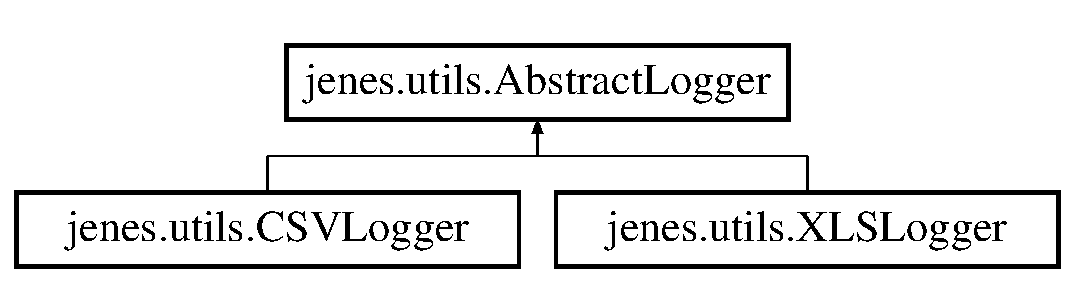
\includegraphics[height=2cm]{classjenes_1_1utils_1_1_abstract_logger}
\end{center}
\end{figure}
\subsection*{Public Member Functions}
\begin{CompactItemize}
\item 
\hyperlink{classjenes_1_1utils_1_1_abstract_logger_357a64e024ede4da833b79455ba63644}{AbstractLogger} (String\mbox{[}$\,$\mbox{]} \hyperlink{classjenes_1_1utils_1_1_abstract_logger_3a2030876857a0512fae7e0ad400c570}{schema})
\item 
String\mbox{[}$\,$\mbox{]} \hyperlink{classjenes_1_1utils_1_1_abstract_logger_3f4dc79a211f8e01c621d42dec8d4de2}{getSchema} ()
\item 
Iterator$<$ String $>$ \hyperlink{classjenes_1_1utils_1_1_abstract_logger_e939c8578c5342d8f11ff61388ddfd80}{getFields} ()
\item 
final void \hyperlink{classjenes_1_1utils_1_1_abstract_logger_0f00b8fa60e88b7c2834be7cdf1fc07e}{put} (String key, Object value)
\item 
final Object \hyperlink{classjenes_1_1utils_1_1_abstract_logger_cceb0a183912b0ec7fc95554ab2e3001}{get} (String key)
\item 
boolean \hyperlink{classjenes_1_1utils_1_1_abstract_logger_f4f01e740a9332b8bb32817e01e7b030}{isRecordComplete} ()
\item 
final void \hyperlink{classjenes_1_1utils_1_1_abstract_logger_26e56f4617fbd249359186c90ec265ba}{log} ()
\item 
void \hyperlink{classjenes_1_1utils_1_1_abstract_logger_736fbff3759196a70dbf6618f10e8786}{save} ()
\item 
void \hyperlink{classjenes_1_1utils_1_1_abstract_logger_7d973cbb6b91f254a5430a8875898dbe}{close} ()
\end{CompactItemize}
\subsection*{Protected Member Functions}
\begin{CompactItemize}
\item 
abstract void \hyperlink{classjenes_1_1utils_1_1_abstract_logger_6acf83a83999e26ae4ed45cbf355111b}{store} ()
\item 
abstract void \hyperlink{classjenes_1_1utils_1_1_abstract_logger_41fcd50b050c467fe1b413fc5b49c167}{doSave} ()
\item 
abstract void \hyperlink{classjenes_1_1utils_1_1_abstract_logger_5253672b3f3f81287db2fc604ca921a9}{doClose} ()
\item 
\hypertarget{classjenes_1_1utils_1_1_abstract_logger_f2c45f653c6e5e79bc4e85dc3ecc4ab4}{
void \textbf{finalize} ()}
\label{classjenes_1_1utils_1_1_abstract_logger_f2c45f653c6e5e79bc4e85dc3ecc4ab4}

\end{CompactItemize}
\subsection*{Protected Attributes}
\begin{CompactItemize}
\item 
List$<$ String $>$ \hyperlink{classjenes_1_1utils_1_1_abstract_logger_3a2030876857a0512fae7e0ad400c570}{schema} = null
\item 
Map$<$ String, Object $>$ \hyperlink{classjenes_1_1utils_1_1_abstract_logger_e85e356ad12255a9c5ec8f9f25659ef7}{record} = new HashMap$<$String, Object$>$()
\item 
\hypertarget{classjenes_1_1utils_1_1_abstract_logger_68fe91d1c7bad9146db3bddd92bbcab3}{
boolean \textbf{closed}}
\label{classjenes_1_1utils_1_1_abstract_logger_68fe91d1c7bad9146db3bddd92bbcab3}

\end{CompactItemize}


\subsection{Detailed Description}
This class provides basic support and interface for logging on different media. A log is made of records. Each record is an associative table of properties.

\begin{Desc}
\item[Version:]2.0 \end{Desc}
\begin{Desc}
\item[Since:]1.3 \end{Desc}


\subsection{Constructor \& Destructor Documentation}
\hypertarget{classjenes_1_1utils_1_1_abstract_logger_357a64e024ede4da833b79455ba63644}{
\index{jenes::utils::AbstractLogger@{jenes::utils::AbstractLogger}!AbstractLogger@{AbstractLogger}}
\index{AbstractLogger@{AbstractLogger}!jenes::utils::AbstractLogger@{jenes::utils::AbstractLogger}}
\subsubsection[AbstractLogger]{\setlength{\rightskip}{0pt plus 5cm}jenes.utils.AbstractLogger.AbstractLogger (String\mbox{[}$\,$\mbox{]} {\em schema})}}
\label{classjenes_1_1utils_1_1_abstract_logger_357a64e024ede4da833b79455ba63644}


Creates a new logger providing a schema

\begin{Desc}
\item[Parameters:]
\begin{description}
\item[{\em schema}]- the logging schema \end{description}
\end{Desc}


\subsection{Member Function Documentation}
\hypertarget{classjenes_1_1utils_1_1_abstract_logger_3f4dc79a211f8e01c621d42dec8d4de2}{
\index{jenes::utils::AbstractLogger@{jenes::utils::AbstractLogger}!getSchema@{getSchema}}
\index{getSchema@{getSchema}!jenes::utils::AbstractLogger@{jenes::utils::AbstractLogger}}
\subsubsection[getSchema]{\setlength{\rightskip}{0pt plus 5cm}String \mbox{[}$\,$\mbox{]} jenes.utils.AbstractLogger.getSchema ()}}
\label{classjenes_1_1utils_1_1_abstract_logger_3f4dc79a211f8e01c621d42dec8d4de2}


Returns the logging schema

\begin{Desc}
\item[Returns:]the array of fields \end{Desc}
\hypertarget{classjenes_1_1utils_1_1_abstract_logger_e939c8578c5342d8f11ff61388ddfd80}{
\index{jenes::utils::AbstractLogger@{jenes::utils::AbstractLogger}!getFields@{getFields}}
\index{getFields@{getFields}!jenes::utils::AbstractLogger@{jenes::utils::AbstractLogger}}
\subsubsection[getFields]{\setlength{\rightskip}{0pt plus 5cm}Iterator$<$String$>$ jenes.utils.AbstractLogger.getFields ()}}
\label{classjenes_1_1utils_1_1_abstract_logger_e939c8578c5342d8f11ff61388ddfd80}


Returns the list of schema fields

\begin{Desc}
\item[Returns:]the iterator of fields \end{Desc}
\hypertarget{classjenes_1_1utils_1_1_abstract_logger_0f00b8fa60e88b7c2834be7cdf1fc07e}{
\index{jenes::utils::AbstractLogger@{jenes::utils::AbstractLogger}!put@{put}}
\index{put@{put}!jenes::utils::AbstractLogger@{jenes::utils::AbstractLogger}}
\subsubsection[put]{\setlength{\rightskip}{0pt plus 5cm}final void jenes.utils.AbstractLogger.put (String {\em key}, \/  Object {\em value})}}
\label{classjenes_1_1utils_1_1_abstract_logger_0f00b8fa60e88b7c2834be7cdf1fc07e}


Puts a value into the current record.

\begin{Desc}
\item[Parameters:]
\begin{description}
\item[{\em key}]- the statistics name \item[{\em value}]- the statistics value \end{description}
\end{Desc}
\hypertarget{classjenes_1_1utils_1_1_abstract_logger_cceb0a183912b0ec7fc95554ab2e3001}{
\index{jenes::utils::AbstractLogger@{jenes::utils::AbstractLogger}!get@{get}}
\index{get@{get}!jenes::utils::AbstractLogger@{jenes::utils::AbstractLogger}}
\subsubsection[get]{\setlength{\rightskip}{0pt plus 5cm}final Object jenes.utils.AbstractLogger.get (String {\em key})}}
\label{classjenes_1_1utils_1_1_abstract_logger_cceb0a183912b0ec7fc95554ab2e3001}


Retrieves a statistics from the current record.

\begin{Desc}
\item[Parameters:]
\begin{description}
\item[{\em key}]- the statistics name \end{description}
\end{Desc}
\begin{Desc}
\item[Returns:]the statistics value \end{Desc}
\hypertarget{classjenes_1_1utils_1_1_abstract_logger_f4f01e740a9332b8bb32817e01e7b030}{
\index{jenes::utils::AbstractLogger@{jenes::utils::AbstractLogger}!isRecordComplete@{isRecordComplete}}
\index{isRecordComplete@{isRecordComplete}!jenes::utils::AbstractLogger@{jenes::utils::AbstractLogger}}
\subsubsection[isRecordComplete]{\setlength{\rightskip}{0pt plus 5cm}boolean jenes.utils.AbstractLogger.isRecordComplete ()}}
\label{classjenes_1_1utils_1_1_abstract_logger_f4f01e740a9332b8bb32817e01e7b030}


Returns true if the record is complete

\begin{Desc}
\item[Returns:]true if the record is complete \end{Desc}
\hypertarget{classjenes_1_1utils_1_1_abstract_logger_26e56f4617fbd249359186c90ec265ba}{
\index{jenes::utils::AbstractLogger@{jenes::utils::AbstractLogger}!log@{log}}
\index{log@{log}!jenes::utils::AbstractLogger@{jenes::utils::AbstractLogger}}
\subsubsection[log]{\setlength{\rightskip}{0pt plus 5cm}final void jenes.utils.AbstractLogger.log ()}}
\label{classjenes_1_1utils_1_1_abstract_logger_26e56f4617fbd249359186c90ec265ba}


Logs a current record by storing it and making the record empty. This is the method to invoke to store the current recorrd. \hypertarget{classjenes_1_1utils_1_1_abstract_logger_736fbff3759196a70dbf6618f10e8786}{
\index{jenes::utils::AbstractLogger@{jenes::utils::AbstractLogger}!save@{save}}
\index{save@{save}!jenes::utils::AbstractLogger@{jenes::utils::AbstractLogger}}
\subsubsection[save]{\setlength{\rightskip}{0pt plus 5cm}void jenes.utils.AbstractLogger.save ()}}
\label{classjenes_1_1utils_1_1_abstract_logger_736fbff3759196a70dbf6618f10e8786}


Saves cached records on media. If the logger is closed this operation is not allowed. \hypertarget{classjenes_1_1utils_1_1_abstract_logger_7d973cbb6b91f254a5430a8875898dbe}{
\index{jenes::utils::AbstractLogger@{jenes::utils::AbstractLogger}!close@{close}}
\index{close@{close}!jenes::utils::AbstractLogger@{jenes::utils::AbstractLogger}}
\subsubsection[close]{\setlength{\rightskip}{0pt plus 5cm}void jenes.utils.AbstractLogger.close ()}}
\label{classjenes_1_1utils_1_1_abstract_logger_7d973cbb6b91f254a5430a8875898dbe}


Saves cached records on media and closes the logger. If the logger is closed this operation is not allowed. \hypertarget{classjenes_1_1utils_1_1_abstract_logger_6acf83a83999e26ae4ed45cbf355111b}{
\index{jenes::utils::AbstractLogger@{jenes::utils::AbstractLogger}!store@{store}}
\index{store@{store}!jenes::utils::AbstractLogger@{jenes::utils::AbstractLogger}}
\subsubsection[store]{\setlength{\rightskip}{0pt plus 5cm}abstract void jenes.utils.AbstractLogger.store ()\hspace{0.3cm}{\tt  \mbox{[}protected, pure virtual\mbox{]}}}}
\label{classjenes_1_1utils_1_1_abstract_logger_6acf83a83999e26ae4ed45cbf355111b}


Stores the current record. 

Implemented in \hyperlink{classjenes_1_1utils_1_1_c_s_v_logger_863bcfda3e93b023949a81e7f6d149e7}{jenes.utils.CSVLogger}, and \hyperlink{classjenes_1_1utils_1_1_x_l_s_logger_e6b3840ad6be8bdc558efaf6077d4ae4}{jenes.utils.XLSLogger}.\hypertarget{classjenes_1_1utils_1_1_abstract_logger_41fcd50b050c467fe1b413fc5b49c167}{
\index{jenes::utils::AbstractLogger@{jenes::utils::AbstractLogger}!doSave@{doSave}}
\index{doSave@{doSave}!jenes::utils::AbstractLogger@{jenes::utils::AbstractLogger}}
\subsubsection[doSave]{\setlength{\rightskip}{0pt plus 5cm}abstract void jenes.utils.AbstractLogger.doSave ()\hspace{0.3cm}{\tt  \mbox{[}protected, pure virtual\mbox{]}}}}
\label{classjenes_1_1utils_1_1_abstract_logger_41fcd50b050c467fe1b413fc5b49c167}


Saves cached records on media 

Implemented in \hyperlink{classjenes_1_1utils_1_1_c_s_v_logger_09a4f4fc362db6d4090d75642521ee65}{jenes.utils.CSVLogger}, and \hyperlink{classjenes_1_1utils_1_1_x_l_s_logger_54c54393bf5a31442ebfc10517dfceea}{jenes.utils.XLSLogger}.\hypertarget{classjenes_1_1utils_1_1_abstract_logger_5253672b3f3f81287db2fc604ca921a9}{
\index{jenes::utils::AbstractLogger@{jenes::utils::AbstractLogger}!doClose@{doClose}}
\index{doClose@{doClose}!jenes::utils::AbstractLogger@{jenes::utils::AbstractLogger}}
\subsubsection[doClose]{\setlength{\rightskip}{0pt plus 5cm}abstract void jenes.utils.AbstractLogger.doClose ()\hspace{0.3cm}{\tt  \mbox{[}protected, pure virtual\mbox{]}}}}
\label{classjenes_1_1utils_1_1_abstract_logger_5253672b3f3f81287db2fc604ca921a9}


Closes the logger. Any further log is not allowed. 

Implemented in \hyperlink{classjenes_1_1utils_1_1_c_s_v_logger_c89f6fe5bd609fcc02ca7adf1407f279}{jenes.utils.CSVLogger}, and \hyperlink{classjenes_1_1utils_1_1_x_l_s_logger_cf58ddaa6873bcf626c9d24064a89b73}{jenes.utils.XLSLogger}.

\subsection{Member Data Documentation}
\hypertarget{classjenes_1_1utils_1_1_abstract_logger_3a2030876857a0512fae7e0ad400c570}{
\index{jenes::utils::AbstractLogger@{jenes::utils::AbstractLogger}!schema@{schema}}
\index{schema@{schema}!jenes::utils::AbstractLogger@{jenes::utils::AbstractLogger}}
\subsubsection[schema]{\setlength{\rightskip}{0pt plus 5cm}List$<$String$>$ {\bf jenes.utils.AbstractLogger.schema} = null\hspace{0.3cm}{\tt  \mbox{[}protected\mbox{]}}}}
\label{classjenes_1_1utils_1_1_abstract_logger_3a2030876857a0512fae7e0ad400c570}


The statistics schema \hypertarget{classjenes_1_1utils_1_1_abstract_logger_e85e356ad12255a9c5ec8f9f25659ef7}{
\index{jenes::utils::AbstractLogger@{jenes::utils::AbstractLogger}!record@{record}}
\index{record@{record}!jenes::utils::AbstractLogger@{jenes::utils::AbstractLogger}}
\subsubsection[record]{\setlength{\rightskip}{0pt plus 5cm}Map$<$String, Object$>$ {\bf jenes.utils.AbstractLogger.record} = new HashMap$<$String, Object$>$()\hspace{0.3cm}{\tt  \mbox{[}protected\mbox{]}}}}
\label{classjenes_1_1utils_1_1_abstract_logger_e85e356ad12255a9c5ec8f9f25659ef7}


The table of value to store. It is the current record to fill. 

The documentation for this class was generated from the following file:\begin{CompactItemize}
\item 
src/jenes/utils/AbstractLogger.java\end{CompactItemize}

\hypertarget{classjenes_1_1stage_1_1_abstract_stage_3_01_t_01extends_01_chromosome_01_4}{
\section{jenes.stage.AbstractStage$<$ T extends Chromosome $>$ Class Reference}
\label{classjenes_1_1stage_1_1_abstract_stage_3_01_t_01extends_01_chromosome_01_4}\index{jenes::stage::AbstractStage$<$ T extends Chromosome $>$@{jenes::stage::AbstractStage$<$ T extends Chromosome $>$}}
}
\subsection*{Public Member Functions}
\begin{CompactItemize}
\item 
abstract void \hyperlink{classjenes_1_1stage_1_1_abstract_stage_3_01_t_01extends_01_chromosome_01_4_1e8398b28d820dc0e7343b15ce19c703}{process} (Population$<$ T $>$ in, Population$<$ T $>$ out)  throws StageException
\item 
void \hyperlink{classjenes_1_1stage_1_1_abstract_stage_3_01_t_01extends_01_chromosome_01_4_f16b278b3f7a6d9fd78e742621b956e5}{init} (GeneticAlgorithm$<$ T $>$ \hyperlink{classjenes_1_1stage_1_1_abstract_stage_3_01_t_01extends_01_chromosome_01_4_751aba4f46b29d22592d48422ffa75f9}{ga})  throws StageException 
\item 
void \hyperlink{classjenes_1_1stage_1_1_abstract_stage_3_01_t_01extends_01_chromosome_01_4_68d4104c004b50abf7b12ffc94122ddc}{dispose} ()  throws StageException 
\item 
boolean \hyperlink{classjenes_1_1stage_1_1_abstract_stage_3_01_t_01extends_01_chromosome_01_4_c20363682ebc9214d9253ff157a06a2d}{isBiggerBetter} ()
\item 
void \hyperlink{classjenes_1_1stage_1_1_abstract_stage_3_01_t_01extends_01_chromosome_01_4_dfddd6664c7f9f2eeba94d59de6fcebf}{setBiggerIsBetter} (boolean flags)
\item 
void \hyperlink{classjenes_1_1stage_1_1_abstract_stage_3_01_t_01extends_01_chromosome_01_4_003250025de6f005e247a05b107e5e8f}{setBiggerIsBetter} (boolean flag, boolean recursively)
\item 
final Fitness$<$ T $>$ \hyperlink{classjenes_1_1stage_1_1_abstract_stage_3_01_t_01extends_01_chromosome_01_4_9de5f0a09b7791fe1e93123ada1c434a}{getFitness} ()
\item 
void \hyperlink{classjenes_1_1stage_1_1_abstract_stage_3_01_t_01extends_01_chromosome_01_4_d60267d0a803c2991ac3ef02ababef2b}{setFitness} (Fitness$<$ T $>$ fit)
\item 
void \hyperlink{classjenes_1_1stage_1_1_abstract_stage_3_01_t_01extends_01_chromosome_01_4_ff1c8307dc89c4fcf7f253b50a87464d}{setFitness} (Fitness$<$ T $>$ fit, boolean recursively)
\item 
boolean \hyperlink{classjenes_1_1stage_1_1_abstract_stage_3_01_t_01extends_01_chromosome_01_4_811a041cd505ad8400b3c8b2aa36f4a9}{isFitnessChanged} ()
\end{CompactItemize}
\subsection*{Protected Attributes}
\begin{CompactItemize}
\item 
GeneticAlgorithm$<$ T $>$ \hyperlink{classjenes_1_1stage_1_1_abstract_stage_3_01_t_01extends_01_chromosome_01_4_751aba4f46b29d22592d48422ffa75f9}{ga}
\item 
boolean \hyperlink{classjenes_1_1stage_1_1_abstract_stage_3_01_t_01extends_01_chromosome_01_4_11da35af3fe950eef9882b03e13690d4}{biggerIsBetter} = true
\item 
Fitness$<$ T $>$ \hyperlink{classjenes_1_1stage_1_1_abstract_stage_3_01_t_01extends_01_chromosome_01_4_697ab8239c1ae2a99445cd7f5fbca45d}{fitness} = null
\end{CompactItemize}


\subsection{Detailed Description}
A generic genetic algorithm stage.\par
 \par
 In Jenes the genetic algorithm body is a \char`\"{}pipe\char`\"{} of stages: each stage processes the input population and produces the output population.\par
 A genetic algoritm invokes the \hyperlink{}{process(Population, Population)} method of each stage. \par
 It is important to consider that the output population is pre-initialized with recicled individuals (for performance reasons), so \hyperlink{}{process(Population, Population)} generally doesn't allocate new Individuals but only changes the genome of that in the output population. The default output population size is equal to the input one, but the stage can (if needed) add or remove individuals from the output population. \par
\par
 Note: a stage can modify the input population. So input passed to process method can be mutated when the process method ends.

\begin{Desc}
\item[Parameters:]
\begin{description}
\item[{\em $<$T$>$}]The class chromosomes flowing across the stage.\end{description}
\end{Desc}
\begin{Desc}
\item[Version:]2.0 \end{Desc}
\begin{Desc}
\item[Since:]1.0 \end{Desc}


\subsection{Member Function Documentation}
\hypertarget{classjenes_1_1stage_1_1_abstract_stage_3_01_t_01extends_01_chromosome_01_4_1e8398b28d820dc0e7343b15ce19c703}{
\index{jenes::stage::AbstractStage$<$ T extends Chromosome $>$@{jenes::stage::AbstractStage$<$ T extends Chromosome $>$}!process@{process}}
\index{process@{process}!jenes::stage::AbstractStage< T extends Chromosome >@{jenes::stage::AbstractStage$<$ T extends Chromosome $>$}}
\subsubsection[process]{\setlength{\rightskip}{0pt plus 5cm}abstract void jenes.stage.AbstractStage$<$ T extends Chromosome $>$.process (Population$<$ T $>$ {\em in}, \/  Population$<$ T $>$ {\em out})  throws {\bf StageException}\hspace{0.3cm}{\tt  \mbox{[}pure virtual\mbox{]}}}}
\label{classjenes_1_1stage_1_1_abstract_stage_3_01_t_01extends_01_chromosome_01_4_1e8398b28d820dc0e7343b15ce19c703}


Processes the input population and tranforms it into the output population. Note:\begin{itemize}
\item Out population is made of recicled individuals. There is a need of new individuals to add only when there is a need to increase the population size. For pre-initalized individual just use setAs method. This is done for an efficient memory management.\item A stage can modify the input population. So input passed to process method can be mutated when the process method ends. \end{itemize}


\begin{Desc}
\item[Parameters:]
\begin{description}
\item[{\em in}]the input population \item[{\em out}]the output population \end{description}
\end{Desc}
\begin{Desc}
\item[Exceptions:]
\begin{description}
\item[{\em \hyperlink{classjenes_1_1stage_1_1_stage_exception}{StageException}}]\end{description}
\end{Desc}
\hypertarget{classjenes_1_1stage_1_1_abstract_stage_3_01_t_01extends_01_chromosome_01_4_f16b278b3f7a6d9fd78e742621b956e5}{
\index{jenes::stage::AbstractStage$<$ T extends Chromosome $>$@{jenes::stage::AbstractStage$<$ T extends Chromosome $>$}!init@{init}}
\index{init@{init}!jenes::stage::AbstractStage< T extends Chromosome >@{jenes::stage::AbstractStage$<$ T extends Chromosome $>$}}
\subsubsection[init]{\setlength{\rightskip}{0pt plus 5cm}void jenes.stage.AbstractStage$<$ T extends Chromosome $>$.init (GeneticAlgorithm$<$ T $>$ {\em ga})  throws {\bf StageException} }}
\label{classjenes_1_1stage_1_1_abstract_stage_3_01_t_01extends_01_chromosome_01_4_f16b278b3f7a6d9fd78e742621b956e5}


Initializes this stage according to the genetic algorithm that uses it

\begin{Desc}
\item[Parameters:]
\begin{description}
\item[{\em ga}]the Genetic Algorithm in wchic this stage run \end{description}
\end{Desc}
\begin{Desc}
\item[Exceptions:]
\begin{description}
\item[{\em \hyperlink{classjenes_1_1stage_1_1_stage_exception}{StageException}}]\end{description}
\end{Desc}
\hypertarget{classjenes_1_1stage_1_1_abstract_stage_3_01_t_01extends_01_chromosome_01_4_68d4104c004b50abf7b12ffc94122ddc}{
\index{jenes::stage::AbstractStage$<$ T extends Chromosome $>$@{jenes::stage::AbstractStage$<$ T extends Chromosome $>$}!dispose@{dispose}}
\index{dispose@{dispose}!jenes::stage::AbstractStage< T extends Chromosome >@{jenes::stage::AbstractStage$<$ T extends Chromosome $>$}}
\subsubsection[dispose]{\setlength{\rightskip}{0pt plus 5cm}void jenes.stage.AbstractStage$<$ T extends Chromosome $>$.dispose ()  throws {\bf StageException} }}
\label{classjenes_1_1stage_1_1_abstract_stage_3_01_t_01extends_01_chromosome_01_4_68d4104c004b50abf7b12ffc94122ddc}


Disposes this stage

\begin{Desc}
\item[Exceptions:]
\begin{description}
\item[{\em \hyperlink{classjenes_1_1stage_1_1_stage_exception}{StageException}}]\end{description}
\end{Desc}
\hypertarget{classjenes_1_1stage_1_1_abstract_stage_3_01_t_01extends_01_chromosome_01_4_c20363682ebc9214d9253ff157a06a2d}{
\index{jenes::stage::AbstractStage$<$ T extends Chromosome $>$@{jenes::stage::AbstractStage$<$ T extends Chromosome $>$}!isBiggerBetter@{isBiggerBetter}}
\index{isBiggerBetter@{isBiggerBetter}!jenes::stage::AbstractStage< T extends Chromosome >@{jenes::stage::AbstractStage$<$ T extends Chromosome $>$}}
\subsubsection[isBiggerBetter]{\setlength{\rightskip}{0pt plus 5cm}boolean jenes.stage.AbstractStage$<$ T extends Chromosome $>$.isBiggerBetter ()}}
\label{classjenes_1_1stage_1_1_abstract_stage_3_01_t_01extends_01_chromosome_01_4_c20363682ebc9214d9253ff157a06a2d}


\begin{Desc}
\item[\hyperlink{deprecated__deprecated000001}{Deprecated}]deprecated due to the use of \hyperlink{}{Fitness}. In next releasese this method will be removed Says if the best individuals have the higher fitness or not.\end{Desc}
\begin{Desc}
\item[Returns:]{\tt true} if the best individuals have the higher fitness$>$ {\tt false} otherwise \end{Desc}
\hypertarget{classjenes_1_1stage_1_1_abstract_stage_3_01_t_01extends_01_chromosome_01_4_dfddd6664c7f9f2eeba94d59de6fcebf}{
\index{jenes::stage::AbstractStage$<$ T extends Chromosome $>$@{jenes::stage::AbstractStage$<$ T extends Chromosome $>$}!setBiggerIsBetter@{setBiggerIsBetter}}
\index{setBiggerIsBetter@{setBiggerIsBetter}!jenes::stage::AbstractStage< T extends Chromosome >@{jenes::stage::AbstractStage$<$ T extends Chromosome $>$}}
\subsubsection[setBiggerIsBetter]{\setlength{\rightskip}{0pt plus 5cm}void jenes.stage.AbstractStage$<$ T extends Chromosome $>$.setBiggerIsBetter (boolean {\em flags})}}
\label{classjenes_1_1stage_1_1_abstract_stage_3_01_t_01extends_01_chromosome_01_4_dfddd6664c7f9f2eeba94d59de6fcebf}


\begin{Desc}
\item[\hyperlink{deprecated__deprecated000002}{Deprecated}]deprecated due to the use of \hyperlink{}{Fitness}. In next releasese this method will be removed Sets if the best individuals have the higher fitness or not. For maximization, this property is set to true; for minimization, this property is set to false. This setting is propagated down to every sub-stage the stage is made of.\end{Desc}
\begin{Desc}
\item[Parameters:]
\begin{description}
\item[{\em flag}]true, if the best individual has the higher fitness \end{description}
\end{Desc}
\hypertarget{classjenes_1_1stage_1_1_abstract_stage_3_01_t_01extends_01_chromosome_01_4_003250025de6f005e247a05b107e5e8f}{
\index{jenes::stage::AbstractStage$<$ T extends Chromosome $>$@{jenes::stage::AbstractStage$<$ T extends Chromosome $>$}!setBiggerIsBetter@{setBiggerIsBetter}}
\index{setBiggerIsBetter@{setBiggerIsBetter}!jenes::stage::AbstractStage< T extends Chromosome >@{jenes::stage::AbstractStage$<$ T extends Chromosome $>$}}
\subsubsection[setBiggerIsBetter]{\setlength{\rightskip}{0pt plus 5cm}void jenes.stage.AbstractStage$<$ T extends Chromosome $>$.setBiggerIsBetter (boolean {\em flag}, \/  boolean {\em recursively})}}
\label{classjenes_1_1stage_1_1_abstract_stage_3_01_t_01extends_01_chromosome_01_4_003250025de6f005e247a05b107e5e8f}


\begin{Desc}
\item[\hyperlink{deprecated__deprecated000003}{Deprecated}]deprecated due to the use of \hyperlink{}{Fitness}. In next releasese this method will be removed Sets if the best individuals have the higher fitness or not. This setting can be or not propagated down to sub-stages.\end{Desc}
\begin{Desc}
\item[Parameters:]
\begin{description}
\item[{\em flag}]true, if the best individual has the higher fitness \item[{\em recursively}]true, to propagate this setting down, otherwise false. \end{description}
\end{Desc}
\hypertarget{classjenes_1_1stage_1_1_abstract_stage_3_01_t_01extends_01_chromosome_01_4_9de5f0a09b7791fe1e93123ada1c434a}{
\index{jenes::stage::AbstractStage$<$ T extends Chromosome $>$@{jenes::stage::AbstractStage$<$ T extends Chromosome $>$}!getFitness@{getFitness}}
\index{getFitness@{getFitness}!jenes::stage::AbstractStage< T extends Chromosome >@{jenes::stage::AbstractStage$<$ T extends Chromosome $>$}}
\subsubsection[getFitness]{\setlength{\rightskip}{0pt plus 5cm}final Fitness$<$T$>$ jenes.stage.AbstractStage$<$ T extends Chromosome $>$.getFitness ()}}
\label{classjenes_1_1stage_1_1_abstract_stage_3_01_t_01extends_01_chromosome_01_4_9de5f0a09b7791fe1e93123ada1c434a}


Get the \hyperlink{}{Fitness} currently setted for this stage \begin{Desc}
\item[Returns:]\end{Desc}
\hypertarget{classjenes_1_1stage_1_1_abstract_stage_3_01_t_01extends_01_chromosome_01_4_d60267d0a803c2991ac3ef02ababef2b}{
\index{jenes::stage::AbstractStage$<$ T extends Chromosome $>$@{jenes::stage::AbstractStage$<$ T extends Chromosome $>$}!setFitness@{setFitness}}
\index{setFitness@{setFitness}!jenes::stage::AbstractStage< T extends Chromosome >@{jenes::stage::AbstractStage$<$ T extends Chromosome $>$}}
\subsubsection[setFitness]{\setlength{\rightskip}{0pt plus 5cm}void jenes.stage.AbstractStage$<$ T extends Chromosome $>$.setFitness (Fitness$<$ T $>$ {\em fit})}}
\label{classjenes_1_1stage_1_1_abstract_stage_3_01_t_01extends_01_chromosome_01_4_d60267d0a803c2991ac3ef02ababef2b}


Change the \hyperlink{}{Fitness} to this stage propagating the change recursively \begin{Desc}
\item[Parameters:]
\begin{description}
\item[{\em fit}]\end{description}
\end{Desc}
\hypertarget{classjenes_1_1stage_1_1_abstract_stage_3_01_t_01extends_01_chromosome_01_4_ff1c8307dc89c4fcf7f253b50a87464d}{
\index{jenes::stage::AbstractStage$<$ T extends Chromosome $>$@{jenes::stage::AbstractStage$<$ T extends Chromosome $>$}!setFitness@{setFitness}}
\index{setFitness@{setFitness}!jenes::stage::AbstractStage< T extends Chromosome >@{jenes::stage::AbstractStage$<$ T extends Chromosome $>$}}
\subsubsection[setFitness]{\setlength{\rightskip}{0pt plus 5cm}void jenes.stage.AbstractStage$<$ T extends Chromosome $>$.setFitness (Fitness$<$ T $>$ {\em fit}, \/  boolean {\em recursively})}}
\label{classjenes_1_1stage_1_1_abstract_stage_3_01_t_01extends_01_chromosome_01_4_ff1c8307dc89c4fcf7f253b50a87464d}


Change the \hyperlink{}{Fitness} to this stage propagating the change recursively according to the flag given as parameter \begin{Desc}
\item[Parameters:]
\begin{description}
\item[{\em fit}]\item[{\em recursively}]\end{description}
\end{Desc}
\hypertarget{classjenes_1_1stage_1_1_abstract_stage_3_01_t_01extends_01_chromosome_01_4_811a041cd505ad8400b3c8b2aa36f4a9}{
\index{jenes::stage::AbstractStage$<$ T extends Chromosome $>$@{jenes::stage::AbstractStage$<$ T extends Chromosome $>$}!isFitnessChanged@{isFitnessChanged}}
\index{isFitnessChanged@{isFitnessChanged}!jenes::stage::AbstractStage< T extends Chromosome >@{jenes::stage::AbstractStage$<$ T extends Chromosome $>$}}
\subsubsection[isFitnessChanged]{\setlength{\rightskip}{0pt plus 5cm}boolean jenes.stage.AbstractStage$<$ T extends Chromosome $>$.isFitnessChanged ()}}
\label{classjenes_1_1stage_1_1_abstract_stage_3_01_t_01extends_01_chromosome_01_4_811a041cd505ad8400b3c8b2aa36f4a9}


Test if the fitness is recently changed \begin{Desc}
\item[Returns:]\end{Desc}


\subsection{Member Data Documentation}
\hypertarget{classjenes_1_1stage_1_1_abstract_stage_3_01_t_01extends_01_chromosome_01_4_751aba4f46b29d22592d48422ffa75f9}{
\index{jenes::stage::AbstractStage$<$ T extends Chromosome $>$@{jenes::stage::AbstractStage$<$ T extends Chromosome $>$}!ga@{ga}}
\index{ga@{ga}!jenes::stage::AbstractStage< T extends Chromosome >@{jenes::stage::AbstractStage$<$ T extends Chromosome $>$}}
\subsubsection[ga]{\setlength{\rightskip}{0pt plus 5cm}GeneticAlgorithm$<$T$>$ jenes.stage.AbstractStage$<$ T extends Chromosome $>$.{\bf ga}\hspace{0.3cm}{\tt  \mbox{[}protected\mbox{]}}}}
\label{classjenes_1_1stage_1_1_abstract_stage_3_01_t_01extends_01_chromosome_01_4_751aba4f46b29d22592d48422ffa75f9}


The genetic algorithm, this stage belongs to \hypertarget{classjenes_1_1stage_1_1_abstract_stage_3_01_t_01extends_01_chromosome_01_4_11da35af3fe950eef9882b03e13690d4}{
\index{jenes::stage::AbstractStage$<$ T extends Chromosome $>$@{jenes::stage::AbstractStage$<$ T extends Chromosome $>$}!biggerIsBetter@{biggerIsBetter}}
\index{biggerIsBetter@{biggerIsBetter}!jenes::stage::AbstractStage< T extends Chromosome >@{jenes::stage::AbstractStage$<$ T extends Chromosome $>$}}
\subsubsection[biggerIsBetter]{\setlength{\rightskip}{0pt plus 5cm}boolean jenes.stage.AbstractStage$<$ T extends Chromosome $>$.{\bf biggerIsBetter} = true\hspace{0.3cm}{\tt  \mbox{[}protected\mbox{]}}}}
\label{classjenes_1_1stage_1_1_abstract_stage_3_01_t_01extends_01_chromosome_01_4_11da35af3fe950eef9882b03e13690d4}


True if higher scores entail better individuals \hypertarget{classjenes_1_1stage_1_1_abstract_stage_3_01_t_01extends_01_chromosome_01_4_697ab8239c1ae2a99445cd7f5fbca45d}{
\index{jenes::stage::AbstractStage$<$ T extends Chromosome $>$@{jenes::stage::AbstractStage$<$ T extends Chromosome $>$}!fitness@{fitness}}
\index{fitness@{fitness}!jenes::stage::AbstractStage< T extends Chromosome >@{jenes::stage::AbstractStage$<$ T extends Chromosome $>$}}
\subsubsection[fitness]{\setlength{\rightskip}{0pt plus 5cm}Fitness$<$T$>$ jenes.stage.AbstractStage$<$ T extends Chromosome $>$.{\bf fitness} = null\hspace{0.3cm}{\tt  \mbox{[}protected\mbox{]}}}}
\label{classjenes_1_1stage_1_1_abstract_stage_3_01_t_01extends_01_chromosome_01_4_697ab8239c1ae2a99445cd7f5fbca45d}


The current Fitness 

The documentation for this class was generated from the following file:\begin{CompactItemize}
\item 
src/jenes/stage/AbstractStage.java\end{CompactItemize}

\hypertarget{interfacejenes_1_1_algorithm_event_listener_3_01_t_01extends_01_chromosome_01_4}{
\section{jenes.AlgorithmEventListener$<$ T extends Chromosome $>$ Interface Reference}
\label{interfacejenes_1_1_algorithm_event_listener_3_01_t_01extends_01_chromosome_01_4}\index{jenes::AlgorithmEventListener$<$ T extends Chromosome $>$@{jenes::AlgorithmEventListener$<$ T extends Chromosome $>$}}
}
\subsection*{Public Member Functions}
\begin{CompactItemize}
\item 
void \hyperlink{interfacejenes_1_1_algorithm_event_listener_3_01_t_01extends_01_chromosome_01_4_f0d6e9961e685f4d44270a4feedeb70f}{onAlgorithmStart} (GeneticAlgorithm$<$ T $>$ ga, long time)
\item 
void \hyperlink{interfacejenes_1_1_algorithm_event_listener_3_01_t_01extends_01_chromosome_01_4_b494ea60f6000ebcd02a94c7eda70dcf}{onAlgorithmStop} (GeneticAlgorithm$<$ T $>$ ga, long time)
\item 
void \hyperlink{interfacejenes_1_1_algorithm_event_listener_3_01_t_01extends_01_chromosome_01_4_f5f6bb7f487c9ecd01331427a370889e}{onAlgorithmInit} (GeneticAlgorithm$<$ T $>$ ga, long time)
\end{CompactItemize}


\subsection{Detailed Description}
{\tt AlgorithmEventListener} provides the interface for capturing events at algorithm level. This iterface should be implemented by all classes interested in being notified by algorithm events, that are: \begin{itemize}
\item Start, when the algorithm evolution starts. The first step consists in initiliazing data structures, in particular populations. \item Init, when the initilization task is accomplished. \item Stop, when the evolution terminates. \end{itemize}


An {\tt AlgorithmEventListener} is registered to the algorithm by the method \hyperlink{}{GeneticAlgorithm\#addAlgorithmEventListener(AlgorithmEventListener)}. The listener is removed by invoking the method \hyperlink{}{GeneticAlgorithm\#removeAlgorithmEventListener(AlgorithmEventListener)}.  

An {\tt AlgorithmEventListener{\tt  can be registered to multiple different algorithms, thus being notified by all of them. }}

{\tt {\tt  Another way to get notified of algorithms events is to override methods \hyperlink{}{GeneticAlgorithm\#onStart(long)}, \hyperlink{}{GeneticAlgorithm\#onInit(long)} and \hyperlink{}{GeneticAlgorithm\#onStop(long)} when subclassing the {\tt GeneticAlgorithm} class. }}

{\tt {\tt  \begin{Desc}
\item[Parameters:]
\begin{description}
\item[{\em $<$T$>$}]extends Chromosome\end{description}
\end{Desc}
\begin{Desc}
\item[Version:]1.2 \end{Desc}
\begin{Desc}
\item[Since:]1.0\end{Desc}
\begin{Desc}
\item[See also:]GeneticAlgorithm \end{Desc}
}}

\subsection{Member Function Documentation}
\hypertarget{interfacejenes_1_1_algorithm_event_listener_3_01_t_01extends_01_chromosome_01_4_f0d6e9961e685f4d44270a4feedeb70f}{
\index{jenes::AlgorithmEventListener$<$ T extends Chromosome $>$@{jenes::AlgorithmEventListener$<$ T extends Chromosome $>$}!onAlgorithmStart@{onAlgorithmStart}}
\index{onAlgorithmStart@{onAlgorithmStart}!jenes::AlgorithmEventListener< T extends Chromosome >@{jenes::AlgorithmEventListener$<$ T extends Chromosome $>$}}
\subsubsection[onAlgorithmStart]{\setlength{\rightskip}{0pt plus 5cm}void jenes.AlgorithmEventListener$<$ T extends Chromosome $>$.onAlgorithmStart (GeneticAlgorithm$<$ T $>$ {\em ga}, \/  long {\em time})}}
\label{interfacejenes_1_1_algorithm_event_listener_3_01_t_01extends_01_chromosome_01_4_f0d6e9961e685f4d44270a4feedeb70f}


Invoked when the genetic algorithm starts

\begin{Desc}
\item[Parameters:]
\begin{description}
\item[{\em ga}]the genetic algorithm that generated this event. \item[{\em time}]the event time expressed in milliseconds \end{description}
\end{Desc}
\hypertarget{interfacejenes_1_1_algorithm_event_listener_3_01_t_01extends_01_chromosome_01_4_b494ea60f6000ebcd02a94c7eda70dcf}{
\index{jenes::AlgorithmEventListener$<$ T extends Chromosome $>$@{jenes::AlgorithmEventListener$<$ T extends Chromosome $>$}!onAlgorithmStop@{onAlgorithmStop}}
\index{onAlgorithmStop@{onAlgorithmStop}!jenes::AlgorithmEventListener< T extends Chromosome >@{jenes::AlgorithmEventListener$<$ T extends Chromosome $>$}}
\subsubsection[onAlgorithmStop]{\setlength{\rightskip}{0pt plus 5cm}void jenes.AlgorithmEventListener$<$ T extends Chromosome $>$.onAlgorithmStop (GeneticAlgorithm$<$ T $>$ {\em ga}, \/  long {\em time})}}
\label{interfacejenes_1_1_algorithm_event_listener_3_01_t_01extends_01_chromosome_01_4_b494ea60f6000ebcd02a94c7eda70dcf}


Invoked when the genetic algorithm ends

\begin{Desc}
\item[Parameters:]
\begin{description}
\item[{\em ga}]the genetic algorithm that generated this event. \item[{\em time}]the event time expressed in milliseconds \end{description}
\end{Desc}
\hypertarget{interfacejenes_1_1_algorithm_event_listener_3_01_t_01extends_01_chromosome_01_4_f5f6bb7f487c9ecd01331427a370889e}{
\index{jenes::AlgorithmEventListener$<$ T extends Chromosome $>$@{jenes::AlgorithmEventListener$<$ T extends Chromosome $>$}!onAlgorithmInit@{onAlgorithmInit}}
\index{onAlgorithmInit@{onAlgorithmInit}!jenes::AlgorithmEventListener< T extends Chromosome >@{jenes::AlgorithmEventListener$<$ T extends Chromosome $>$}}
\subsubsection[onAlgorithmInit]{\setlength{\rightskip}{0pt plus 5cm}void jenes.AlgorithmEventListener$<$ T extends Chromosome $>$.onAlgorithmInit (GeneticAlgorithm$<$ T $>$ {\em ga}, \/  long {\em time})}}
\label{interfacejenes_1_1_algorithm_event_listener_3_01_t_01extends_01_chromosome_01_4_f5f6bb7f487c9ecd01331427a370889e}


Invoked when the genetic algorithm is initialized

\begin{Desc}
\item[Parameters:]
\begin{description}
\item[{\em ga}]the genetic algorithm that generated this event. \item[{\em time}]the event time expressed in milliseconds \end{description}
\end{Desc}


The documentation for this interface was generated from the following file:\begin{CompactItemize}
\item 
src/jenes/AlgorithmEventListener.java\end{CompactItemize}

\hypertarget{classjenes_1_1_algorithm_exception}{
\section{jenes.AlgorithmException Class Reference}
\label{classjenes_1_1_algorithm_exception}\index{jenes::AlgorithmException@{jenes::AlgorithmException}}
}
\subsection*{Public Member Functions}
\begin{CompactItemize}
\item 
\hyperlink{classjenes_1_1_algorithm_exception_a53d271c0db7099eb6fc52c288e05eb0}{AlgorithmException} (String msg, Throwable cause)
\item 
\hyperlink{classjenes_1_1_algorithm_exception_295c243603f7b36f9ab5b0e1ec22aa60}{AlgorithmException} (String msg)
\item 
\hyperlink{classjenes_1_1_algorithm_exception_d6906756121d65db53ece1c1d9d8d0db}{AlgorithmException} (Throwable cause)
\end{CompactItemize}


\subsection{Detailed Description}
An {\tt \hyperlink{classjenes_1_1_algorithm_exception}{AlgorithmException}} is a runtime exception thrown during the algorithm execution.

\begin{Desc}
\item[Version:]1.2 \end{Desc}
\begin{Desc}
\item[Since:]1.0 \end{Desc}


\subsection{Constructor \& Destructor Documentation}
\hypertarget{classjenes_1_1_algorithm_exception_a53d271c0db7099eb6fc52c288e05eb0}{
\index{jenes::AlgorithmException@{jenes::AlgorithmException}!AlgorithmException@{AlgorithmException}}
\index{AlgorithmException@{AlgorithmException}!jenes::AlgorithmException@{jenes::AlgorithmException}}
\subsubsection[AlgorithmException]{\setlength{\rightskip}{0pt plus 5cm}jenes.AlgorithmException.AlgorithmException (String {\em msg}, \/  Throwable {\em cause})}}
\label{classjenes_1_1_algorithm_exception_a53d271c0db7099eb6fc52c288e05eb0}


Creates an {\tt \hyperlink{classjenes_1_1_algorithm_exception}{AlgorithmException}} providing an error message and an exception cause.

\begin{Desc}
\item[Parameters:]
\begin{description}
\item[{\em msg}]the error message \item[{\em cause}]the error cause \end{description}
\end{Desc}
\hypertarget{classjenes_1_1_algorithm_exception_295c243603f7b36f9ab5b0e1ec22aa60}{
\index{jenes::AlgorithmException@{jenes::AlgorithmException}!AlgorithmException@{AlgorithmException}}
\index{AlgorithmException@{AlgorithmException}!jenes::AlgorithmException@{jenes::AlgorithmException}}
\subsubsection[AlgorithmException]{\setlength{\rightskip}{0pt plus 5cm}jenes.AlgorithmException.AlgorithmException (String {\em msg})}}
\label{classjenes_1_1_algorithm_exception_295c243603f7b36f9ab5b0e1ec22aa60}


Creates an {\tt \hyperlink{classjenes_1_1_algorithm_exception}{AlgorithmException}} providing only an error message

\begin{Desc}
\item[Parameters:]
\begin{description}
\item[{\em msg}]the error message \end{description}
\end{Desc}
\hypertarget{classjenes_1_1_algorithm_exception_d6906756121d65db53ece1c1d9d8d0db}{
\index{jenes::AlgorithmException@{jenes::AlgorithmException}!AlgorithmException@{AlgorithmException}}
\index{AlgorithmException@{AlgorithmException}!jenes::AlgorithmException@{jenes::AlgorithmException}}
\subsubsection[AlgorithmException]{\setlength{\rightskip}{0pt plus 5cm}jenes.AlgorithmException.AlgorithmException (Throwable {\em cause})}}
\label{classjenes_1_1_algorithm_exception_d6906756121d65db53ece1c1d9d8d0db}


Creates an {\tt \hyperlink{classjenes_1_1_algorithm_exception}{AlgorithmException}} providing an exception cause, and no additional message.

\begin{Desc}
\item[Parameters:]
\begin{description}
\item[{\em cause}]the error cause \end{description}
\end{Desc}


The documentation for this class was generated from the following file:\begin{CompactItemize}
\item 
src/jenes/AlgorithmException.java\end{CompactItemize}

\hypertarget{classjenes_1_1stage_1_1_algorithm_stage_3_01_t_01extends_01_chromosome_01_4}{
\section{jenes.stage.AlgorithmStage$<$ T extends Chromosome $>$ Class Reference}
\label{classjenes_1_1stage_1_1_algorithm_stage_3_01_t_01extends_01_chromosome_01_4}\index{jenes::stage::AlgorithmStage$<$ T extends Chromosome $>$@{jenes::stage::AlgorithmStage$<$ T extends Chromosome $>$}}
}
Inherits jenes::stage::AbstractStage$<$ T $>$.

\subsection*{Public Member Functions}
\begin{CompactItemize}
\item 
\hyperlink{classjenes_1_1stage_1_1_algorithm_stage_3_01_t_01extends_01_chromosome_01_4_802871d36189757fc869c5a542dc1b9c}{AlgorithmStage} (GeneticAlgorithm$<$ T $>$ algorithm)
\item 
final GeneticAlgorithm$<$ T $>$ \hyperlink{classjenes_1_1stage_1_1_algorithm_stage_3_01_t_01extends_01_chromosome_01_4_7c1be30eb9852c0f16031f3802d770aa}{getAlgorithm} ()
\item 
\hypertarget{classjenes_1_1stage_1_1_algorithm_stage_3_01_t_01extends_01_chromosome_01_4_5d27c95b7872fc28cc7b78be601dd9d0}{
void \textbf{setBiggerIsBetter} (boolean flag, boolean recursively)}
\label{classjenes_1_1stage_1_1_algorithm_stage_3_01_t_01extends_01_chromosome_01_4_5d27c95b7872fc28cc7b78be601dd9d0}

\item 
\hypertarget{classjenes_1_1stage_1_1_algorithm_stage_3_01_t_01extends_01_chromosome_01_4_43c9964c60c539aaea0193c9552b262b}{
void \textbf{setFitness} (Fitness fit, boolean recursively)}
\label{classjenes_1_1stage_1_1_algorithm_stage_3_01_t_01extends_01_chromosome_01_4_43c9964c60c539aaea0193c9552b262b}

\item 
\hypertarget{classjenes_1_1stage_1_1_algorithm_stage_3_01_t_01extends_01_chromosome_01_4_43a7b7271f320f04c8be69bfdafb078e}{
void \textbf{process} (Population$<$ T $>$ in, Population$<$ T $>$ out)  throws StageException }
\label{classjenes_1_1stage_1_1_algorithm_stage_3_01_t_01extends_01_chromosome_01_4_43a7b7271f320f04c8be69bfdafb078e}

\end{CompactItemize}


\subsection{Detailed Description}
A stage wrapping an algoithm in order to make it part of a wider algorithm.

\begin{Desc}
\item[Parameters:]
\begin{description}
\item[{\em $<$T$>$}]The class chromosomes flowing across the stage.\end{description}
\end{Desc}
\begin{Desc}
\item[Version:]2.0 \end{Desc}
\begin{Desc}
\item[Since:]1.3 \end{Desc}


\subsection{Constructor \& Destructor Documentation}
\hypertarget{classjenes_1_1stage_1_1_algorithm_stage_3_01_t_01extends_01_chromosome_01_4_802871d36189757fc869c5a542dc1b9c}{
\index{jenes::stage::AlgorithmStage$<$ T extends Chromosome $>$@{jenes::stage::AlgorithmStage$<$ T extends Chromosome $>$}!AlgorithmStage@{AlgorithmStage}}
\index{AlgorithmStage@{AlgorithmStage}!jenes::stage::AlgorithmStage< T extends Chromosome >@{jenes::stage::AlgorithmStage$<$ T extends Chromosome $>$}}
\subsubsection[AlgorithmStage]{\setlength{\rightskip}{0pt plus 5cm}jenes.stage.AlgorithmStage$<$ T extends Chromosome $>$.AlgorithmStage (GeneticAlgorithm$<$ T $>$ {\em algorithm})}}
\label{classjenes_1_1stage_1_1_algorithm_stage_3_01_t_01extends_01_chromosome_01_4_802871d36189757fc869c5a542dc1b9c}


Builds a wrapper stage for the specified algorithm.

\begin{Desc}
\item[Parameters:]
\begin{description}
\item[{\em algorithm}]the algorithm to wrap. \end{description}
\end{Desc}


\subsection{Member Function Documentation}
\hypertarget{classjenes_1_1stage_1_1_algorithm_stage_3_01_t_01extends_01_chromosome_01_4_7c1be30eb9852c0f16031f3802d770aa}{
\index{jenes::stage::AlgorithmStage$<$ T extends Chromosome $>$@{jenes::stage::AlgorithmStage$<$ T extends Chromosome $>$}!getAlgorithm@{getAlgorithm}}
\index{getAlgorithm@{getAlgorithm}!jenes::stage::AlgorithmStage< T extends Chromosome >@{jenes::stage::AlgorithmStage$<$ T extends Chromosome $>$}}
\subsubsection[getAlgorithm]{\setlength{\rightskip}{0pt plus 5cm}final GeneticAlgorithm$<$T$>$ jenes.stage.AlgorithmStage$<$ T extends Chromosome $>$.getAlgorithm ()}}
\label{classjenes_1_1stage_1_1_algorithm_stage_3_01_t_01extends_01_chromosome_01_4_7c1be30eb9852c0f16031f3802d770aa}


Returns the wrapped algorithm

\begin{Desc}
\item[Returns:]the algorithm \end{Desc}


The documentation for this class was generated from the following file:\begin{CompactItemize}
\item 
src/jenes/stage/AlgorithmStage.java\end{CompactItemize}

\hypertarget{interfacejenes_1_1chromosome_1_1_allele_set_3_01_t_01_4}{
\section{jenes.chromosome.AlleleSet$<$ T $>$ Interface Reference}
\label{interfacejenes_1_1chromosome_1_1_allele_set_3_01_t_01_4}\index{jenes::chromosome::AlleleSet$<$ T $>$@{jenes::chromosome::AlleleSet$<$ T $>$}}
}
Inheritance diagram for jenes.chromosome.AlleleSet$<$ T $>$::\begin{figure}[H]
\begin{center}
\leavevmode
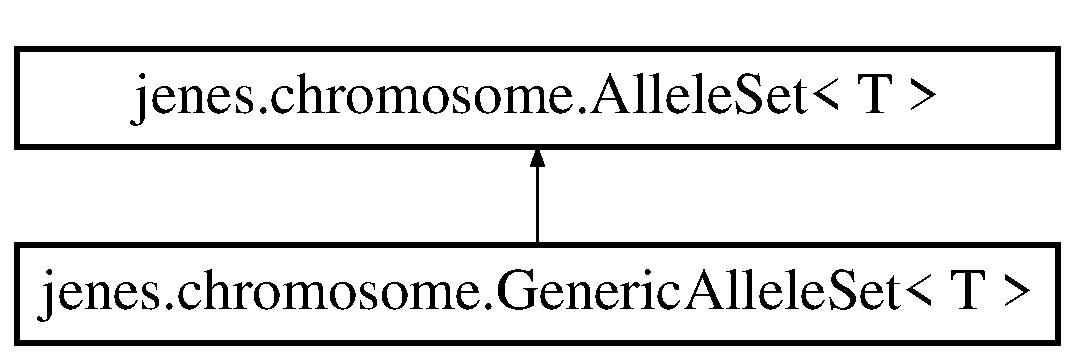
\includegraphics[height=2cm]{interfacejenes_1_1chromosome_1_1_allele_set_3_01_t_01_4}
\end{center}
\end{figure}
\subsection*{Public Member Functions}
\begin{CompactItemize}
\item 
abstract T \hyperlink{interfacejenes_1_1chromosome_1_1_allele_set_3_01_t_01_4_10625403643dc57a5c655a92a49aa644}{getElementAt} (int pos)
\item 
abstract T \hyperlink{interfacejenes_1_1chromosome_1_1_allele_set_3_01_t_01_4_c09d409c55d941892df658d21b3d4bff}{getRandomValue} ()
\item 
abstract int \hyperlink{interfacejenes_1_1chromosome_1_1_allele_set_3_01_t_01_4_3acbb10df92ebafc589d5d8546949f2f}{size} ()
\item 
abstract double \hyperlink{interfacejenes_1_1chromosome_1_1_allele_set_3_01_t_01_4_74ab0cb120fcfdee8e878727d6c50815}{difference} (T a0, T a1)
\end{CompactItemize}


\subsection{Detailed Description}
An AlleleSet represents an alphabet of object gene allele values. Each \hyperlink{}{ObjectChromosome.Gene} of an \hyperlink{classjenes_1_1chromosome_1_1_object_chromosome}{ObjectChromosome} has an allele set containing all the object values it can assume. A custom set of values can be determined by implementing this interface.

\begin{Desc}
\item[Parameters:]
\begin{description}
\item[{\em $<$T$>$}]class of elements held by AlleleSet\end{description}
\end{Desc}
\begin{Desc}
\item[Version:]2.0 \end{Desc}
\begin{Desc}
\item[Since:]1.0\end{Desc}
\begin{Desc}
\item[See also:]\hyperlink{classjenes_1_1chromosome_1_1_object_chromosome}{jenes.chromosome.ObjectChromosome} \end{Desc}


\subsection{Member Function Documentation}
\hypertarget{interfacejenes_1_1chromosome_1_1_allele_set_3_01_t_01_4_10625403643dc57a5c655a92a49aa644}{
\index{jenes::chromosome::AlleleSet$<$ T $>$@{jenes::chromosome::AlleleSet$<$ T $>$}!getElementAt@{getElementAt}}
\index{getElementAt@{getElementAt}!jenes::chromosome::AlleleSet< T >@{jenes::chromosome::AlleleSet$<$ T $>$}}
\subsubsection[getElementAt]{\setlength{\rightskip}{0pt plus 5cm}abstract T jenes.chromosome.AlleleSet$<$ T $>$.getElementAt (int {\em pos})\hspace{0.3cm}{\tt  \mbox{[}pure virtual\mbox{]}}}}
\label{interfacejenes_1_1chromosome_1_1_allele_set_3_01_t_01_4_10625403643dc57a5c655a92a49aa644}


Gets the allele value at the specified position 

\begin{Desc}
\item[Parameters:]
\begin{description}
\item[{\em pos}]the index of the desidered allele value \end{description}
\end{Desc}
\begin{Desc}
\item[Returns:]the allele value at the specified position \end{Desc}
\hypertarget{interfacejenes_1_1chromosome_1_1_allele_set_3_01_t_01_4_c09d409c55d941892df658d21b3d4bff}{
\index{jenes::chromosome::AlleleSet$<$ T $>$@{jenes::chromosome::AlleleSet$<$ T $>$}!getRandomValue@{getRandomValue}}
\index{getRandomValue@{getRandomValue}!jenes::chromosome::AlleleSet< T >@{jenes::chromosome::AlleleSet$<$ T $>$}}
\subsubsection[getRandomValue]{\setlength{\rightskip}{0pt plus 5cm}abstract T jenes.chromosome.AlleleSet$<$ T $>$.getRandomValue ()\hspace{0.3cm}{\tt  \mbox{[}pure virtual\mbox{]}}}}
\label{interfacejenes_1_1chromosome_1_1_allele_set_3_01_t_01_4_c09d409c55d941892df658d21b3d4bff}


Gets a random allele value within this alphabet. The allele value returned has to be a copy of the value in the allele set. 

\begin{Desc}
\item[Returns:]the random value selected \end{Desc}


Implemented in \hyperlink{classjenes_1_1chromosome_1_1_generic_allele_set_3_01_t_01_4_2f330d71d992e0d724bc31730b56229e}{jenes.chromosome.GenericAlleleSet$<$ T $>$}.\hypertarget{interfacejenes_1_1chromosome_1_1_allele_set_3_01_t_01_4_3acbb10df92ebafc589d5d8546949f2f}{
\index{jenes::chromosome::AlleleSet$<$ T $>$@{jenes::chromosome::AlleleSet$<$ T $>$}!size@{size}}
\index{size@{size}!jenes::chromosome::AlleleSet< T >@{jenes::chromosome::AlleleSet$<$ T $>$}}
\subsubsection[size]{\setlength{\rightskip}{0pt plus 5cm}abstract int jenes.chromosome.AlleleSet$<$ T $>$.size ()\hspace{0.3cm}{\tt  \mbox{[}pure virtual\mbox{]}}}}
\label{interfacejenes_1_1chromosome_1_1_allele_set_3_01_t_01_4_3acbb10df92ebafc589d5d8546949f2f}


Returns the alphabet size 

\begin{Desc}
\item[Returns:]the alphabet size \end{Desc}


Implemented in \hyperlink{classjenes_1_1chromosome_1_1_generic_allele_set_3_01_t_01_4_568ca617716496507d41e348c5bc2845}{jenes.chromosome.GenericAlleleSet$<$ T $>$}.\hypertarget{interfacejenes_1_1chromosome_1_1_allele_set_3_01_t_01_4_74ab0cb120fcfdee8e878727d6c50815}{
\index{jenes::chromosome::AlleleSet$<$ T $>$@{jenes::chromosome::AlleleSet$<$ T $>$}!difference@{difference}}
\index{difference@{difference}!jenes::chromosome::AlleleSet< T >@{jenes::chromosome::AlleleSet$<$ T $>$}}
\subsubsection[difference]{\setlength{\rightskip}{0pt plus 5cm}abstract double jenes.chromosome.AlleleSet$<$ T $>$.difference (T {\em a0}, \/  T {\em a1})\hspace{0.3cm}{\tt  \mbox{[}pure virtual\mbox{]}}}}
\label{interfacejenes_1_1chromosome_1_1_allele_set_3_01_t_01_4_74ab0cb120fcfdee8e878727d6c50815}


Provides the genetic difference between two alleles.

\begin{Desc}
\item[Parameters:]
\begin{description}
\item[{\em a0}]- first allele \item[{\em a1}]- second allele \end{description}
\end{Desc}
\begin{Desc}
\item[Returns:]- the genetic difeerence \end{Desc}


Implemented in \hyperlink{classjenes_1_1chromosome_1_1_generic_allele_set_3_01_t_01_4_ce70b10ee535ccc3a7cbcd42739b8d5c}{jenes.chromosome.GenericAlleleSet$<$ T $>$}.

The documentation for this interface was generated from the following file:\begin{CompactItemize}
\item 
src/jenes/chromosome/AlleleSet.java\end{CompactItemize}

\hypertarget{classjenes_1_1chromosome_1_1_bitwise_chromosome}{
\section{jenes.chromosome.BitwiseChromosome Class Reference}
\label{classjenes_1_1chromosome_1_1_bitwise_chromosome}\index{jenes::chromosome::BitwiseChromosome@{jenes::chromosome::BitwiseChromosome}}
}
Inherits jenes::chromosome::Chromosome$<$ jenes::chromosome::BitwiseChromosome $>$.

\subsection*{Public Types}
\begin{CompactItemize}
\item 
enum \hyperlink{classjenes_1_1chromosome_1_1_bitwise_chromosome_dcebd2053ddb9906f17a29837e6ff04c}{BitSize} \{ \hyperlink{_bitwise_chromosome_8java_dcebd2053ddb9906f17a29837e6ff04c4982bc4d3de52713a035a54a501149f8}{BIT1} = (1, 0x1), 
\hyperlink{_bitwise_chromosome_8java_dcebd2053ddb9906f17a29837e6ff04cf64ab504b0994d78a4d72bba097ffaec}{BIT8} = (8, 0xFF), 
\hyperlink{_bitwise_chromosome_8java_dcebd2053ddb9906f17a29837e6ff04c12b7defe5ace4d6bd26b7c9d0881689d}{BIT16} = (16, 0xFFFF), 
\hyperlink{_bitwise_chromosome_8java_dcebd2053ddb9906f17a29837e6ff04cf738d5c01006c83629e2cd1f04a6889a}{BIT32} = (32, 0xFFFFFFFF)
 \}
\end{CompactItemize}
\subsection*{Public Member Functions}
\begin{CompactItemize}
\item 
\hyperlink{classjenes_1_1chromosome_1_1_bitwise_chromosome_87547c87419943bded51820cbc1ae830}{BitwiseChromosome} (final int size)
\item 
\hyperlink{classjenes_1_1chromosome_1_1_bitwise_chromosome_9109a8205e447db9032f29494f0d9b3d}{BitwiseChromosome} (final int size, final BitCoding coding)
\item 
\hyperlink{classjenes_1_1chromosome_1_1_bitwise_chromosome_90798d86b6c1871c441b562e0b1d50ca}{BitwiseChromosome} (final \hyperlink{classjenes_1_1chromosome_1_1_bitwise_chromosome}{BitwiseChromosome} chromosome)
\item 
final BitCoding \hyperlink{classjenes_1_1chromosome_1_1_bitwise_chromosome_905b92cd6dc14db9d2b9276f1a6686e9}{getType} ()
\item 
final int \hyperlink{classjenes_1_1chromosome_1_1_bitwise_chromosome_e59ae8f495ec9d5aa15712cee7c0b313}{getSize} ()
\item 
final int \hyperlink{classjenes_1_1chromosome_1_1_bitwise_chromosome_f817cb2110fc6b8d415e46377ddd4911}{getIntValueAt} (final int index)
\item 
final void \hyperlink{classjenes_1_1chromosome_1_1_bitwise_chromosome_3cbcf428333a0dc4209ce2c820054542}{setIntValueAt} (final int index, final int value)
\item 
final int \hyperlink{classjenes_1_1chromosome_1_1_bitwise_chromosome_36e6b8c849d563a359245763116667d5}{getIntSize} ()
\item 
final Object \hyperlink{classjenes_1_1chromosome_1_1_bitwise_chromosome_3061d34e1f0c0faa915d4da7ea2f615c}{getValueAt} (final int index)
\item 
final void \hyperlink{classjenes_1_1chromosome_1_1_bitwise_chromosome_aa42be8f0c26735e8a8d603d9b743b6a}{setValue} (final int index, final Object value)
\item 
final int \hyperlink{classjenes_1_1chromosome_1_1_bitwise_chromosome_05ce80f3729d007c5d550eef5969ac86}{getBitValueAt} (final int index)
\item 
final void \hyperlink{classjenes_1_1chromosome_1_1_bitwise_chromosome_2e746b511933914d4be452573ac5ab7c}{setBitValueAt} (final int index, final int bit)
\item 
final void \hyperlink{classjenes_1_1chromosome_1_1_bitwise_chromosome_2d711baa2a74ccb064d33ef73edbd464}{cross} (final \hyperlink{classjenes_1_1chromosome_1_1_bitwise_chromosome}{BitwiseChromosome} chromosome, final int from, final int to)
\item 
final void \hyperlink{classjenes_1_1chromosome_1_1_bitwise_chromosome_933b1991999fa3b586c1739744751725}{cross} (final \hyperlink{classjenes_1_1chromosome_1_1_bitwise_chromosome}{BitwiseChromosome} chromosome, final int from)
\item 
final boolean \hyperlink{classjenes_1_1chromosome_1_1_bitwise_chromosome_41c9858f7ef05194011d1e227fea3584}{equals} (final \hyperlink{classjenes_1_1chromosome_1_1_bitwise_chromosome}{BitwiseChromosome} chromosome)
\item 
final int \hyperlink{classjenes_1_1chromosome_1_1_bitwise_chromosome_0da8899c89f8b1f222526acf1d2e8519}{length} ()
\item 
final int \hyperlink{classjenes_1_1chromosome_1_1_bitwise_chromosome_5878e8d0ace81cfb617f75109c02855d}{getIntLength} ()
\item 
final void \hyperlink{classjenes_1_1chromosome_1_1_bitwise_chromosome_1a79d4c9c671d2f735d57d64c59dfdb8}{randomize} (final int pos)
\item 
final void \hyperlink{classjenes_1_1chromosome_1_1_bitwise_chromosome_8028fde93528b7b51313f6c311b2b640}{randomize} ()
\item 
final void \hyperlink{classjenes_1_1chromosome_1_1_bitwise_chromosome_b02c791be30c931cae793289185e459f}{leftShift} (final int from, final int to)
\item 
final void \hyperlink{classjenes_1_1chromosome_1_1_bitwise_chromosome_fb689c4b268f7954214a9d0e13c6141e}{rightShift} (final int from, final int to)
\item 
final void \hyperlink{classjenes_1_1chromosome_1_1_bitwise_chromosome_a4fbad5a25ae14e9524a6ff0ec2536ca}{setAs} (final \hyperlink{classjenes_1_1chromosome_1_1_bitwise_chromosome}{BitwiseChromosome} chromosome)
\item 
final void \hyperlink{classjenes_1_1chromosome_1_1_bitwise_chromosome_e5be5fc21ff47526230a8a13ca945c08}{setDefaultValueAt} (final int pos)
\item 
final void \hyperlink{classjenes_1_1chromosome_1_1_bitwise_chromosome_fac4935f0e1d92b6b1aaf9de024e8cbb}{swap} (final int pos1, final int pos2)
\item 
final \hyperlink{classjenes_1_1chromosome_1_1_bitwise_chromosome}{BitwiseChromosome} \hyperlink{classjenes_1_1chromosome_1_1_bitwise_chromosome_2140b588068c430eaea7e9a7a5fe6b00}{clone} ()
\item 
\hypertarget{classjenes_1_1chromosome_1_1_bitwise_chromosome_33de872210289a305bc869c61a02eddb}{
void \textbf{difference} (\hyperlink{classjenes_1_1chromosome_1_1_bitwise_chromosome}{BitwiseChromosome} chromosome, double\mbox{[}$\,$\mbox{]} diff)}
\label{classjenes_1_1chromosome_1_1_bitwise_chromosome_33de872210289a305bc869c61a02eddb}

\item 
\hypertarget{classjenes_1_1chromosome_1_1_bitwise_chromosome_a191192f94ce72a631237674d81ae393}{
Object\mbox{[}$\,$\mbox{]} \textbf{toArray} ()}
\label{classjenes_1_1chromosome_1_1_bitwise_chromosome_a191192f94ce72a631237674d81ae393}

\end{CompactItemize}
\subsection*{Classes}
\begin{CompactItemize}
\item 
class \textbf{BitCoding$<$ T $>$}
\end{CompactItemize}


\subsection{Detailed Description}
This class provides chromosomes made of bits. Its genome contains objects coded according to a specified \hyperlink{}{BitCoding}. Typically objects coded by this chromosome are numeric values. The default integer representation is used when no BitCoding is specified. 

A \hyperlink{classjenes_1_1chromosome_1_1_bitwise_chromosome}{BitwiseChromosome} has size and length attributes. The size is the number of coded value contained by its genoma; the length is the number of bits. The length depends on which coding is used for translating objects into bits. The relation between size and length is shown below: 

$<$blockquote$>$\small\begin{alltt}
  aBitwiseChromosome.length() = aBitwiseChromosome.getSize() *  aCoding.SIZE.BITS
 \end{alltt}
\normalsize 
$<$/blockquote$>$ where aCoding.SIZE.BITS is the number of bits required for coding one object. 

This Chromosome performs genetic operations at bit level, processing an array of integer, thus ensuring a high throughput and minimal memory occupation. Using a 16 bit representation, a chromosome holding 4 objects (size) will be represented by 32 bits (length), thus by 2 integers (as each of integer is represented by 32 bit)

\begin{Desc}
\item[Version:]2.0 \end{Desc}
\begin{Desc}
\item[Since:]1.0 \end{Desc}


\subsection{Member Enumeration Documentation}
\hypertarget{classjenes_1_1chromosome_1_1_bitwise_chromosome_dcebd2053ddb9906f17a29837e6ff04c}{
\index{jenes::chromosome::BitwiseChromosome@{jenes::chromosome::BitwiseChromosome}!BitSize@{BitSize}}
\index{BitSize@{BitSize}!jenes::chromosome::BitwiseChromosome@{jenes::chromosome::BitwiseChromosome}}
\subsubsection[BitSize]{\setlength{\rightskip}{0pt plus 5cm}enum {\bf jenes::chromosome::BitwiseChromosome::BitSize}}}
\label{classjenes_1_1chromosome_1_1_bitwise_chromosome_dcebd2053ddb9906f17a29837e6ff04c}


Definition of the number bit length and mask to use in the coding operations.

\begin{Desc}
\item[Author:]Luigi Troiano 

Pierpaolo Lombardi 

Giuseppe Pascale 

Thierry Bodhuin\end{Desc}
\begin{Desc}
\item[Version:]1.2\end{Desc}
\begin{Desc}
\item[Since:]1.0 \end{Desc}


\subsection{Constructor \& Destructor Documentation}
\hypertarget{classjenes_1_1chromosome_1_1_bitwise_chromosome_87547c87419943bded51820cbc1ae830}{
\index{jenes::chromosome::BitwiseChromosome@{jenes::chromosome::BitwiseChromosome}!BitwiseChromosome@{BitwiseChromosome}}
\index{BitwiseChromosome@{BitwiseChromosome}!jenes::chromosome::BitwiseChromosome@{jenes::chromosome::BitwiseChromosome}}
\subsubsection[BitwiseChromosome]{\setlength{\rightskip}{0pt plus 5cm}jenes.chromosome.BitwiseChromosome.BitwiseChromosome (final int {\em size})}}
\label{classjenes_1_1chromosome_1_1_bitwise_chromosome_87547c87419943bded51820cbc1ae830}


Creates a new \hyperlink{classjenes_1_1chromosome_1_1_bitwise_chromosome}{BitwiseChromosome} with the specified number of objects. The chromosome is made of a bit string encoding objects.

\begin{Desc}
\item[Parameters:]
\begin{description}
\item[{\em size}]the number of objects the chromosone represents \end{description}
\end{Desc}
\hypertarget{classjenes_1_1chromosome_1_1_bitwise_chromosome_9109a8205e447db9032f29494f0d9b3d}{
\index{jenes::chromosome::BitwiseChromosome@{jenes::chromosome::BitwiseChromosome}!BitwiseChromosome@{BitwiseChromosome}}
\index{BitwiseChromosome@{BitwiseChromosome}!jenes::chromosome::BitwiseChromosome@{jenes::chromosome::BitwiseChromosome}}
\subsubsection[BitwiseChromosome]{\setlength{\rightskip}{0pt plus 5cm}jenes.chromosome.BitwiseChromosome.BitwiseChromosome (final int {\em size}, \/  final BitCoding {\em coding})}}
\label{classjenes_1_1chromosome_1_1_bitwise_chromosome_9109a8205e447db9032f29494f0d9b3d}


Creates a new \hyperlink{classjenes_1_1chromosome_1_1_bitwise_chromosome}{BitwiseChromosome} with the specified number of objects and coding.

\begin{Desc}
\item[Parameters:]
\begin{description}
\item[{\em size}]the number of chromosome coded objects \item[{\em coding}]the coding to use \end{description}
\end{Desc}
\hypertarget{classjenes_1_1chromosome_1_1_bitwise_chromosome_90798d86b6c1871c441b562e0b1d50ca}{
\index{jenes::chromosome::BitwiseChromosome@{jenes::chromosome::BitwiseChromosome}!BitwiseChromosome@{BitwiseChromosome}}
\index{BitwiseChromosome@{BitwiseChromosome}!jenes::chromosome::BitwiseChromosome@{jenes::chromosome::BitwiseChromosome}}
\subsubsection[BitwiseChromosome]{\setlength{\rightskip}{0pt plus 5cm}jenes.chromosome.BitwiseChromosome.BitwiseChromosome (final {\bf BitwiseChromosome} {\em chromosome})}}
\label{classjenes_1_1chromosome_1_1_bitwise_chromosome_90798d86b6c1871c441b562e0b1d50ca}


Creates a new \hyperlink{classjenes_1_1chromosome_1_1_bitwise_chromosome}{BitwiseChromosome} using the specified one as prototype

\begin{Desc}
\item[Parameters:]
\begin{description}
\item[{\em chromosome}]the chromosome to copy \end{description}
\end{Desc}


\subsection{Member Function Documentation}
\hypertarget{classjenes_1_1chromosome_1_1_bitwise_chromosome_905b92cd6dc14db9d2b9276f1a6686e9}{
\index{jenes::chromosome::BitwiseChromosome@{jenes::chromosome::BitwiseChromosome}!getType@{getType}}
\index{getType@{getType}!jenes::chromosome::BitwiseChromosome@{jenes::chromosome::BitwiseChromosome}}
\subsubsection[getType]{\setlength{\rightskip}{0pt plus 5cm}final BitCoding jenes.chromosome.BitwiseChromosome.getType ()}}
\label{classjenes_1_1chromosome_1_1_bitwise_chromosome_905b92cd6dc14db9d2b9276f1a6686e9}


Returns the \hyperlink{}{BitCoding} used by this chromosome

\begin{Desc}
\item[Returns:]the bit coding used \end{Desc}
\hypertarget{classjenes_1_1chromosome_1_1_bitwise_chromosome_e59ae8f495ec9d5aa15712cee7c0b313}{
\index{jenes::chromosome::BitwiseChromosome@{jenes::chromosome::BitwiseChromosome}!getSize@{getSize}}
\index{getSize@{getSize}!jenes::chromosome::BitwiseChromosome@{jenes::chromosome::BitwiseChromosome}}
\subsubsection[getSize]{\setlength{\rightskip}{0pt plus 5cm}final int jenes.chromosome.BitwiseChromosome.getSize ()}}
\label{classjenes_1_1chromosome_1_1_bitwise_chromosome_e59ae8f495ec9d5aa15712cee7c0b313}


Returns the number of coded objects contained by this chromosome.

\begin{Desc}
\item[Returns:]the number of coded objects \end{Desc}
\hypertarget{classjenes_1_1chromosome_1_1_bitwise_chromosome_f817cb2110fc6b8d415e46377ddd4911}{
\index{jenes::chromosome::BitwiseChromosome@{jenes::chromosome::BitwiseChromosome}!getIntValueAt@{getIntValueAt}}
\index{getIntValueAt@{getIntValueAt}!jenes::chromosome::BitwiseChromosome@{jenes::chromosome::BitwiseChromosome}}
\subsubsection[getIntValueAt]{\setlength{\rightskip}{0pt plus 5cm}final int jenes.chromosome.BitwiseChromosome.getIntValueAt (final int {\em index})}}
\label{classjenes_1_1chromosome_1_1_bitwise_chromosome_f817cb2110fc6b8d415e46377ddd4911}


Returns the int value at the specified position

\begin{Desc}
\item[Parameters:]
\begin{description}
\item[{\em index}]the index of the value to return \end{description}
\end{Desc}
\begin{Desc}
\item[Returns:]the int value at the specified position \end{Desc}
\hypertarget{classjenes_1_1chromosome_1_1_bitwise_chromosome_3cbcf428333a0dc4209ce2c820054542}{
\index{jenes::chromosome::BitwiseChromosome@{jenes::chromosome::BitwiseChromosome}!setIntValueAt@{setIntValueAt}}
\index{setIntValueAt@{setIntValueAt}!jenes::chromosome::BitwiseChromosome@{jenes::chromosome::BitwiseChromosome}}
\subsubsection[setIntValueAt]{\setlength{\rightskip}{0pt plus 5cm}final void jenes.chromosome.BitwiseChromosome.setIntValueAt (final int {\em index}, \/  final int {\em value})}}
\label{classjenes_1_1chromosome_1_1_bitwise_chromosome_3cbcf428333a0dc4209ce2c820054542}


Sets the int value at the specified position

\begin{Desc}
\item[Parameters:]
\begin{description}
\item[{\em index}]the index of the element to be modify \item[{\em value}]the value to set \end{description}
\end{Desc}
\hypertarget{classjenes_1_1chromosome_1_1_bitwise_chromosome_36e6b8c849d563a359245763116667d5}{
\index{jenes::chromosome::BitwiseChromosome@{jenes::chromosome::BitwiseChromosome}!getIntSize@{getIntSize}}
\index{getIntSize@{getIntSize}!jenes::chromosome::BitwiseChromosome@{jenes::chromosome::BitwiseChromosome}}
\subsubsection[getIntSize]{\setlength{\rightskip}{0pt plus 5cm}final int jenes.chromosome.BitwiseChromosome.getIntSize ()}}
\label{classjenes_1_1chromosome_1_1_bitwise_chromosome_36e6b8c849d563a359245763116667d5}


Returns the number of integer used by the chromosome for coding the objects

\begin{Desc}
\item[Returns:]the number of integers \end{Desc}
\hypertarget{classjenes_1_1chromosome_1_1_bitwise_chromosome_3061d34e1f0c0faa915d4da7ea2f615c}{
\index{jenes::chromosome::BitwiseChromosome@{jenes::chromosome::BitwiseChromosome}!getValueAt@{getValueAt}}
\index{getValueAt@{getValueAt}!jenes::chromosome::BitwiseChromosome@{jenes::chromosome::BitwiseChromosome}}
\subsubsection[getValueAt]{\setlength{\rightskip}{0pt plus 5cm}final Object jenes.chromosome.BitwiseChromosome.getValueAt (final int {\em index})}}
\label{classjenes_1_1chromosome_1_1_bitwise_chromosome_3061d34e1f0c0faa915d4da7ea2f615c}


Returns the object value at the specified position in the chromosome. The value is decoded and returned.

\begin{Desc}
\item[Parameters:]
\begin{description}
\item[{\em index}]the position \end{description}
\end{Desc}
\begin{Desc}
\item[Returns:]the object \end{Desc}
\hypertarget{classjenes_1_1chromosome_1_1_bitwise_chromosome_aa42be8f0c26735e8a8d603d9b743b6a}{
\index{jenes::chromosome::BitwiseChromosome@{jenes::chromosome::BitwiseChromosome}!setValue@{setValue}}
\index{setValue@{setValue}!jenes::chromosome::BitwiseChromosome@{jenes::chromosome::BitwiseChromosome}}
\subsubsection[setValue]{\setlength{\rightskip}{0pt plus 5cm}final void jenes.chromosome.BitwiseChromosome.setValue (final int {\em index}, \/  final Object {\em value})}}
\label{classjenes_1_1chromosome_1_1_bitwise_chromosome_aa42be8f0c26735e8a8d603d9b743b6a}


Sets the specified object value at the given position. The object value is encoded and then placed in the chromosome.

\begin{Desc}
\item[Parameters:]
\begin{description}
\item[{\em index}]the position \item[{\em value}]the object value to be placed \end{description}
\end{Desc}
\hypertarget{classjenes_1_1chromosome_1_1_bitwise_chromosome_05ce80f3729d007c5d550eef5969ac86}{
\index{jenes::chromosome::BitwiseChromosome@{jenes::chromosome::BitwiseChromosome}!getBitValueAt@{getBitValueAt}}
\index{getBitValueAt@{getBitValueAt}!jenes::chromosome::BitwiseChromosome@{jenes::chromosome::BitwiseChromosome}}
\subsubsection[getBitValueAt]{\setlength{\rightskip}{0pt plus 5cm}final int jenes.chromosome.BitwiseChromosome.getBitValueAt (final int {\em index})}}
\label{classjenes_1_1chromosome_1_1_bitwise_chromosome_05ce80f3729d007c5d550eef5969ac86}


Returns the bit value at the specified position. This position takes into account the usage of integers made by the coding specification. For instance, if the coding requires 5 bits for each value, index 31 does not point to the last bit of the first integer, but to the second bit of the second integer, as described below

\mbox{[}01101 01110 00011 11011 10101 10010 --\mbox{]} \mbox{[}01100 11010 ...

\begin{Desc}
\item[Parameters:]
\begin{description}
\item[{\em index}]the position \end{description}
\end{Desc}
\begin{Desc}
\item[Returns:]the bit value \end{Desc}
\hypertarget{classjenes_1_1chromosome_1_1_bitwise_chromosome_2e746b511933914d4be452573ac5ab7c}{
\index{jenes::chromosome::BitwiseChromosome@{jenes::chromosome::BitwiseChromosome}!setBitValueAt@{setBitValueAt}}
\index{setBitValueAt@{setBitValueAt}!jenes::chromosome::BitwiseChromosome@{jenes::chromosome::BitwiseChromosome}}
\subsubsection[setBitValueAt]{\setlength{\rightskip}{0pt plus 5cm}final void jenes.chromosome.BitwiseChromosome.setBitValueAt (final int {\em index}, \/  final int {\em bit})}}
\label{classjenes_1_1chromosome_1_1_bitwise_chromosome_2e746b511933914d4be452573ac5ab7c}


Sets the bit at a given position. Position is related to the bits actually used and not to those occupied by the chromosome data structure.

\begin{Desc}
\item[Parameters:]
\begin{description}
\item[{\em index}]the position \item[{\em bit}]the bit value \end{description}
\end{Desc}
\hypertarget{classjenes_1_1chromosome_1_1_bitwise_chromosome_2d711baa2a74ccb064d33ef73edbd464}{
\index{jenes::chromosome::BitwiseChromosome@{jenes::chromosome::BitwiseChromosome}!cross@{cross}}
\index{cross@{cross}!jenes::chromosome::BitwiseChromosome@{jenes::chromosome::BitwiseChromosome}}
\subsubsection[cross]{\setlength{\rightskip}{0pt plus 5cm}final void jenes.chromosome.BitwiseChromosome.cross (final {\bf BitwiseChromosome} {\em chromosome}, \/  final int {\em from}, \/  final int {\em to})}}
\label{classjenes_1_1chromosome_1_1_bitwise_chromosome_2d711baa2a74ccb064d33ef73edbd464}


Exchanges the chromosome bits in the range \mbox{[}from,to\mbox{]}. The range is referred to positions of bits effectively used by the chromosome and not to thoae occupied by the underlying data structure.

\begin{Desc}
\item[Parameters:]
\begin{description}
\item[{\em chromosome}]the chromosome to cross with \item[{\em from}]the initial cross site \item[{\em to}]the final cross site \end{description}
\end{Desc}
\hypertarget{classjenes_1_1chromosome_1_1_bitwise_chromosome_933b1991999fa3b586c1739744751725}{
\index{jenes::chromosome::BitwiseChromosome@{jenes::chromosome::BitwiseChromosome}!cross@{cross}}
\index{cross@{cross}!jenes::chromosome::BitwiseChromosome@{jenes::chromosome::BitwiseChromosome}}
\subsubsection[cross]{\setlength{\rightskip}{0pt plus 5cm}final void jenes.chromosome.BitwiseChromosome.cross (final {\bf BitwiseChromosome} {\em chromosome}, \/  final int {\em from})}}
\label{classjenes_1_1chromosome_1_1_bitwise_chromosome_933b1991999fa3b586c1739744751725}


Exchanges the chromosome bits from the specified cross site to the final position

\begin{Desc}
\item[Parameters:]
\begin{description}
\item[{\em chromosome}]the chromosome to cross with \item[{\em from}]the initial cross site \end{description}
\end{Desc}
\hypertarget{classjenes_1_1chromosome_1_1_bitwise_chromosome_41c9858f7ef05194011d1e227fea3584}{
\index{jenes::chromosome::BitwiseChromosome@{jenes::chromosome::BitwiseChromosome}!equals@{equals}}
\index{equals@{equals}!jenes::chromosome::BitwiseChromosome@{jenes::chromosome::BitwiseChromosome}}
\subsubsection[equals]{\setlength{\rightskip}{0pt plus 5cm}final boolean jenes.chromosome.BitwiseChromosome.equals (final {\bf BitwiseChromosome} {\em chromosome})}}
\label{classjenes_1_1chromosome_1_1_bitwise_chromosome_41c9858f7ef05194011d1e227fea3584}


Compares the chromosome with another.

\begin{Desc}
\item[Parameters:]
\begin{description}
\item[{\em chromosome}]the chromosome to compare to. \end{description}
\end{Desc}
\begin{Desc}
\item[Returns:]true, if the two chromosome are equal. \end{Desc}
\hypertarget{classjenes_1_1chromosome_1_1_bitwise_chromosome_0da8899c89f8b1f222526acf1d2e8519}{
\index{jenes::chromosome::BitwiseChromosome@{jenes::chromosome::BitwiseChromosome}!length@{length}}
\index{length@{length}!jenes::chromosome::BitwiseChromosome@{jenes::chromosome::BitwiseChromosome}}
\subsubsection[length]{\setlength{\rightskip}{0pt plus 5cm}final int jenes.chromosome.BitwiseChromosome.length ()}}
\label{classjenes_1_1chromosome_1_1_bitwise_chromosome_0da8899c89f8b1f222526acf1d2e8519}


Returns the chromosome length expressed in bits. This value can be different from the effective chromosome length (the latter can contain bits used to make the former multiple of \hyperlink{}{Integer\#SIZE})

\begin{Desc}
\item[Returns:]the chromosome length \end{Desc}
\hypertarget{classjenes_1_1chromosome_1_1_bitwise_chromosome_5878e8d0ace81cfb617f75109c02855d}{
\index{jenes::chromosome::BitwiseChromosome@{jenes::chromosome::BitwiseChromosome}!getIntLength@{getIntLength}}
\index{getIntLength@{getIntLength}!jenes::chromosome::BitwiseChromosome@{jenes::chromosome::BitwiseChromosome}}
\subsubsection[getIntLength]{\setlength{\rightskip}{0pt plus 5cm}final int jenes.chromosome.BitwiseChromosome.getIntLength ()}}
\label{classjenes_1_1chromosome_1_1_bitwise_chromosome_5878e8d0ace81cfb617f75109c02855d}


Returns the chromosome length expressed in integers

\begin{Desc}
\item[Returns:]the number of integers \end{Desc}
\hypertarget{classjenes_1_1chromosome_1_1_bitwise_chromosome_1a79d4c9c671d2f735d57d64c59dfdb8}{
\index{jenes::chromosome::BitwiseChromosome@{jenes::chromosome::BitwiseChromosome}!randomize@{randomize}}
\index{randomize@{randomize}!jenes::chromosome::BitwiseChromosome@{jenes::chromosome::BitwiseChromosome}}
\subsubsection[randomize]{\setlength{\rightskip}{0pt plus 5cm}final void jenes.chromosome.BitwiseChromosome.randomize (final int {\em pos})}}
\label{classjenes_1_1chromosome_1_1_bitwise_chromosome_1a79d4c9c671d2f735d57d64c59dfdb8}


Randomizes the bit at the given position

\begin{Desc}
\item[Parameters:]
\begin{description}
\item[{\em pos}]the position of bit to alter \end{description}
\end{Desc}
\hypertarget{classjenes_1_1chromosome_1_1_bitwise_chromosome_8028fde93528b7b51313f6c311b2b640}{
\index{jenes::chromosome::BitwiseChromosome@{jenes::chromosome::BitwiseChromosome}!randomize@{randomize}}
\index{randomize@{randomize}!jenes::chromosome::BitwiseChromosome@{jenes::chromosome::BitwiseChromosome}}
\subsubsection[randomize]{\setlength{\rightskip}{0pt plus 5cm}final void jenes.chromosome.BitwiseChromosome.randomize ()}}
\label{classjenes_1_1chromosome_1_1_bitwise_chromosome_8028fde93528b7b51313f6c311b2b640}


Randomizes each chromosome bit \hypertarget{classjenes_1_1chromosome_1_1_bitwise_chromosome_b02c791be30c931cae793289185e459f}{
\index{jenes::chromosome::BitwiseChromosome@{jenes::chromosome::BitwiseChromosome}!leftShift@{leftShift}}
\index{leftShift@{leftShift}!jenes::chromosome::BitwiseChromosome@{jenes::chromosome::BitwiseChromosome}}
\subsubsection[leftShift]{\setlength{\rightskip}{0pt plus 5cm}final void jenes.chromosome.BitwiseChromosome.leftShift (final int {\em from}, \/  final int {\em to})}}
\label{classjenes_1_1chromosome_1_1_bitwise_chromosome_b02c791be30c931cae793289185e459f}


Executes the left shift of bits within the specified range. The shift is circular, so the most right-side bit becomes the first bit on left.

\begin{Desc}
\item[Parameters:]
\begin{description}
\item[{\em from}]the lower range limit \item[{\em to}]the upper range limit \end{description}
\end{Desc}
\hypertarget{classjenes_1_1chromosome_1_1_bitwise_chromosome_fb689c4b268f7954214a9d0e13c6141e}{
\index{jenes::chromosome::BitwiseChromosome@{jenes::chromosome::BitwiseChromosome}!rightShift@{rightShift}}
\index{rightShift@{rightShift}!jenes::chromosome::BitwiseChromosome@{jenes::chromosome::BitwiseChromosome}}
\subsubsection[rightShift]{\setlength{\rightskip}{0pt plus 5cm}final void jenes.chromosome.BitwiseChromosome.rightShift (final int {\em from}, \/  final int {\em to})}}
\label{classjenes_1_1chromosome_1_1_bitwise_chromosome_fb689c4b268f7954214a9d0e13c6141e}


Executes the right shift of bits within the specified range. The shift is circular, so the most left-side bit becomes the last bit on right.

\begin{Desc}
\item[Parameters:]
\begin{description}
\item[{\em from}]the lower range limit \item[{\em to}]the upper range limit \end{description}
\end{Desc}
\hypertarget{classjenes_1_1chromosome_1_1_bitwise_chromosome_a4fbad5a25ae14e9524a6ff0ec2536ca}{
\index{jenes::chromosome::BitwiseChromosome@{jenes::chromosome::BitwiseChromosome}!setAs@{setAs}}
\index{setAs@{setAs}!jenes::chromosome::BitwiseChromosome@{jenes::chromosome::BitwiseChromosome}}
\subsubsection[setAs]{\setlength{\rightskip}{0pt plus 5cm}final void jenes.chromosome.BitwiseChromosome.setAs (final {\bf BitwiseChromosome} {\em chromosome})}}
\label{classjenes_1_1chromosome_1_1_bitwise_chromosome_a4fbad5a25ae14e9524a6ff0ec2536ca}


Sets this chromosome as a copy of another.

\begin{Desc}
\item[Parameters:]
\begin{description}
\item[{\em chromosome}]the chromosome to copy \end{description}
\end{Desc}
\hypertarget{classjenes_1_1chromosome_1_1_bitwise_chromosome_e5be5fc21ff47526230a8a13ca945c08}{
\index{jenes::chromosome::BitwiseChromosome@{jenes::chromosome::BitwiseChromosome}!setDefaultValueAt@{setDefaultValueAt}}
\index{setDefaultValueAt@{setDefaultValueAt}!jenes::chromosome::BitwiseChromosome@{jenes::chromosome::BitwiseChromosome}}
\subsubsection[setDefaultValueAt]{\setlength{\rightskip}{0pt plus 5cm}final void jenes.chromosome.BitwiseChromosome.setDefaultValueAt (final int {\em pos})}}
\label{classjenes_1_1chromosome_1_1_bitwise_chromosome_e5be5fc21ff47526230a8a13ca945c08}


Sets the default bit value at the a given position

\begin{Desc}
\item[Parameters:]
\begin{description}
\item[{\em pos}]bit position \end{description}
\end{Desc}
\hypertarget{classjenes_1_1chromosome_1_1_bitwise_chromosome_fac4935f0e1d92b6b1aaf9de024e8cbb}{
\index{jenes::chromosome::BitwiseChromosome@{jenes::chromosome::BitwiseChromosome}!swap@{swap}}
\index{swap@{swap}!jenes::chromosome::BitwiseChromosome@{jenes::chromosome::BitwiseChromosome}}
\subsubsection[swap]{\setlength{\rightskip}{0pt plus 5cm}final void jenes.chromosome.BitwiseChromosome.swap (final int {\em pos1}, \/  final int {\em pos2})}}
\label{classjenes_1_1chromosome_1_1_bitwise_chromosome_fac4935f0e1d92b6b1aaf9de024e8cbb}


Swaps two bits at given positions

\begin{Desc}
\item[Parameters:]
\begin{description}
\item[{\em pos1}]first bit position \item[{\em pos2}]second bit position \end{description}
\end{Desc}
\hypertarget{classjenes_1_1chromosome_1_1_bitwise_chromosome_2140b588068c430eaea7e9a7a5fe6b00}{
\index{jenes::chromosome::BitwiseChromosome@{jenes::chromosome::BitwiseChromosome}!clone@{clone}}
\index{clone@{clone}!jenes::chromosome::BitwiseChromosome@{jenes::chromosome::BitwiseChromosome}}
\subsubsection[clone]{\setlength{\rightskip}{0pt plus 5cm}final {\bf BitwiseChromosome} jenes.chromosome.BitwiseChromosome.clone ()}}
\label{classjenes_1_1chromosome_1_1_bitwise_chromosome_2140b588068c430eaea7e9a7a5fe6b00}


Makes a chromosome copy

\begin{Desc}
\item[Returns:]the chromsome clone \end{Desc}


The documentation for this class was generated from the following file:\begin{CompactItemize}
\item 
src/jenes/chromosome/BitwiseChromosome.java\end{CompactItemize}

\hypertarget{classjenes_1_1chromosome_1_1_boolean_chromosome}{
\section{jenes.chromosome.BooleanChromosome Class Reference}
\label{classjenes_1_1chromosome_1_1_boolean_chromosome}\index{jenes::chromosome::BooleanChromosome@{jenes::chromosome::BooleanChromosome}}
}
Inherits jenes::chromosome::Chromosome$<$ jenes::chromosome::BooleanChromosome $>$.

\subsection*{Public Member Functions}
\begin{CompactItemize}
\item 
\hyperlink{classjenes_1_1chromosome_1_1_boolean_chromosome_dd8b8de56dc676084576bcc657125414}{BooleanChromosome} (final \hyperlink{classjenes_1_1chromosome_1_1_boolean_chromosome}{BooleanChromosome} chromosome)
\item 
\hyperlink{classjenes_1_1chromosome_1_1_boolean_chromosome_ea950688e012d2bfe97f4f24a3fc1db6}{BooleanChromosome} (final int size)
\item 
\hypertarget{classjenes_1_1chromosome_1_1_boolean_chromosome_df2084640bd92e4d36ffea9142e39f8e}{
final void \textbf{setDefaultValueAt} (final int pos)}
\label{classjenes_1_1chromosome_1_1_boolean_chromosome_df2084640bd92e4d36ffea9142e39f8e}

\item 
\hypertarget{classjenes_1_1chromosome_1_1_boolean_chromosome_0f0ea11e413734e15dc659a3d0831801}{
final \hyperlink{classjenes_1_1chromosome_1_1_boolean_chromosome}{BooleanChromosome} \textbf{clone} ()}
\label{classjenes_1_1chromosome_1_1_boolean_chromosome_0f0ea11e413734e15dc659a3d0831801}

\item 
\hypertarget{classjenes_1_1chromosome_1_1_boolean_chromosome_b02039091f6803486d54b4f124a39b63}{
final void \textbf{randomize} ()}
\label{classjenes_1_1chromosome_1_1_boolean_chromosome_b02039091f6803486d54b4f124a39b63}

\item 
\hypertarget{classjenes_1_1chromosome_1_1_boolean_chromosome_f0249c8a5452c3a13960543ab23d4aae}{
final void \textbf{randomize} (final int pos)}
\label{classjenes_1_1chromosome_1_1_boolean_chromosome_f0249c8a5452c3a13960543ab23d4aae}

\item 
\hypertarget{classjenes_1_1chromosome_1_1_boolean_chromosome_6359dc1f495e4f7967c6a84f3206de40}{
final void \textbf{swap} (final int pos1, final int pos2)}
\label{classjenes_1_1chromosome_1_1_boolean_chromosome_6359dc1f495e4f7967c6a84f3206de40}

\item 
\hypertarget{classjenes_1_1chromosome_1_1_boolean_chromosome_96c0fb9c3f1668cbc9ca175a183f69d4}{
final void \textbf{leftShift} (final int from, int to)}
\label{classjenes_1_1chromosome_1_1_boolean_chromosome_96c0fb9c3f1668cbc9ca175a183f69d4}

\item 
\hypertarget{classjenes_1_1chromosome_1_1_boolean_chromosome_866689aeafc1b4a5e83c14a1605bc7ce}{
final void \textbf{rightShift} (final int from, int to)}
\label{classjenes_1_1chromosome_1_1_boolean_chromosome_866689aeafc1b4a5e83c14a1605bc7ce}

\item 
\hypertarget{classjenes_1_1chromosome_1_1_boolean_chromosome_4665770a8e625c26f3704b41fecb10f8}{
final int \textbf{length} ()}
\label{classjenes_1_1chromosome_1_1_boolean_chromosome_4665770a8e625c26f3704b41fecb10f8}

\item 
\hypertarget{classjenes_1_1chromosome_1_1_boolean_chromosome_16d9851ba21583010d003378a7d59d19}{
final void \textbf{setAs} (final \hyperlink{classjenes_1_1chromosome_1_1_boolean_chromosome}{BooleanChromosome} chromosome)}
\label{classjenes_1_1chromosome_1_1_boolean_chromosome_16d9851ba21583010d003378a7d59d19}

\item 
\hypertarget{classjenes_1_1chromosome_1_1_boolean_chromosome_a1c3c421b6e8e6db44fb7cce7443e669}{
final void \textbf{cross} (final \hyperlink{classjenes_1_1chromosome_1_1_boolean_chromosome}{BooleanChromosome} chromosome, final int from)}
\label{classjenes_1_1chromosome_1_1_boolean_chromosome_a1c3c421b6e8e6db44fb7cce7443e669}

\item 
\hypertarget{classjenes_1_1chromosome_1_1_boolean_chromosome_f31ce0ed4f82fccd837cfde93bc4ee61}{
final void \textbf{cross} (final \hyperlink{classjenes_1_1chromosome_1_1_boolean_chromosome}{BooleanChromosome} chromosome, final int from, final int to)}
\label{classjenes_1_1chromosome_1_1_boolean_chromosome_f31ce0ed4f82fccd837cfde93bc4ee61}

\item 
final boolean \hyperlink{classjenes_1_1chromosome_1_1_boolean_chromosome_6edb214f001732cfd6af9bbac3a23515}{getValue} (final int pos)
\item 
final boolean\mbox{[}$\,$\mbox{]} \hyperlink{classjenes_1_1chromosome_1_1_boolean_chromosome_27db9ee77a97d896d0cdafc726681272}{getValues} ()
\item 
final void \hyperlink{classjenes_1_1chromosome_1_1_boolean_chromosome_9bd35e276f2739f19fa7a695c85f415c}{setValueAt} (boolean value, int position)
\item 
final boolean\mbox{[}$\,$\mbox{]} \hyperlink{classjenes_1_1chromosome_1_1_boolean_chromosome_afccb6ebf217d02c0502e185b1972f82}{getValues} (final boolean values\mbox{[}$\,$\mbox{]})
\item 
final void \hyperlink{classjenes_1_1chromosome_1_1_boolean_chromosome_3730cbcd4d048349f134593db820566d}{setDefaultValue} (final boolean defaultValue)
\item 
final boolean \hyperlink{classjenes_1_1chromosome_1_1_boolean_chromosome_9b75f626b2b5fbc90215a53ac91d24a7}{getDefaultValue} ()
\item 
final void \hyperlink{classjenes_1_1chromosome_1_1_boolean_chromosome_b37e05ed7a30e43b740f0c2d9c548e88}{setValue} (final int pos, final boolean value)
\item 
\hypertarget{classjenes_1_1chromosome_1_1_boolean_chromosome_17ecce8325cc2ba6b1703551768c245f}{
final String \textbf{toString} ()}
\label{classjenes_1_1chromosome_1_1_boolean_chromosome_17ecce8325cc2ba6b1703551768c245f}

\item 
\hypertarget{classjenes_1_1chromosome_1_1_boolean_chromosome_82b50fe50a7e8821ee3ae5cc96bca013}{
final boolean \textbf{equals} (final \hyperlink{classjenes_1_1chromosome_1_1_boolean_chromosome}{BooleanChromosome} chromosome)}
\label{classjenes_1_1chromosome_1_1_boolean_chromosome_82b50fe50a7e8821ee3ae5cc96bca013}

\item 
\hypertarget{classjenes_1_1chromosome_1_1_boolean_chromosome_0d602ca5a958ee2712963602d2f1eee9}{
void \textbf{difference} (\hyperlink{classjenes_1_1chromosome_1_1_boolean_chromosome}{BooleanChromosome} chromosome, double\mbox{[}$\,$\mbox{]} diff)}
\label{classjenes_1_1chromosome_1_1_boolean_chromosome_0d602ca5a958ee2712963602d2f1eee9}

\item 
\hypertarget{classjenes_1_1chromosome_1_1_boolean_chromosome_3ff06b819a640b0e89935d99cc69d3ac}{
Object\mbox{[}$\,$\mbox{]} \textbf{toArray} ()}
\label{classjenes_1_1chromosome_1_1_boolean_chromosome_3ff06b819a640b0e89935d99cc69d3ac}

\end{CompactItemize}


\subsection{Detailed Description}
A \hyperlink{classjenes_1_1chromosome_1_1_boolean_chromosome}{BooleanChromosome} is made of an array of booleans. Each gene can assume the value true or false. A faster and less memory demanding alternative to \hyperlink{classjenes_1_1chromosome_1_1_boolean_chromosome}{BooleanChromosome} is provided by \hyperlink{classjenes_1_1chromosome_1_1_bitwise_chromosome}{BitwiseChromosome} with \hyperlink{classjenes_1_1chromosome_1_1codings_1_1_boolean_coding}{jenes.chromosome.codings.BooleanCoding}.

\begin{Desc}
\item[Version:]2.0 \end{Desc}
\begin{Desc}
\item[Since:]1.0 \end{Desc}


\subsection{Constructor \& Destructor Documentation}
\hypertarget{classjenes_1_1chromosome_1_1_boolean_chromosome_dd8b8de56dc676084576bcc657125414}{
\index{jenes::chromosome::BooleanChromosome@{jenes::chromosome::BooleanChromosome}!BooleanChromosome@{BooleanChromosome}}
\index{BooleanChromosome@{BooleanChromosome}!jenes::chromosome::BooleanChromosome@{jenes::chromosome::BooleanChromosome}}
\subsubsection[BooleanChromosome]{\setlength{\rightskip}{0pt plus 5cm}jenes.chromosome.BooleanChromosome.BooleanChromosome (final {\bf BooleanChromosome} {\em chromosome})}}
\label{classjenes_1_1chromosome_1_1_boolean_chromosome_dd8b8de56dc676084576bcc657125414}


Creates a new \hyperlink{classjenes_1_1chromosome_1_1_boolean_chromosome}{BooleanChromosome} with the specified chromosome 

\begin{Desc}
\item[Parameters:]
\begin{description}
\item[{\em chromosome}]the parameters source chromosome \end{description}
\end{Desc}
\hypertarget{classjenes_1_1chromosome_1_1_boolean_chromosome_ea950688e012d2bfe97f4f24a3fc1db6}{
\index{jenes::chromosome::BooleanChromosome@{jenes::chromosome::BooleanChromosome}!BooleanChromosome@{BooleanChromosome}}
\index{BooleanChromosome@{BooleanChromosome}!jenes::chromosome::BooleanChromosome@{jenes::chromosome::BooleanChromosome}}
\subsubsection[BooleanChromosome]{\setlength{\rightskip}{0pt plus 5cm}jenes.chromosome.BooleanChromosome.BooleanChromosome (final int {\em size})}}
\label{classjenes_1_1chromosome_1_1_boolean_chromosome_ea950688e012d2bfe97f4f24a3fc1db6}


Creates a new \hyperlink{classjenes_1_1chromosome_1_1_boolean_chromosome}{BooleanChromosome} with the specified chromosome length 

\begin{Desc}
\item[Parameters:]
\begin{description}
\item[{\em size}]the chromosome length \end{description}
\end{Desc}


\subsection{Member Function Documentation}
\hypertarget{classjenes_1_1chromosome_1_1_boolean_chromosome_6edb214f001732cfd6af9bbac3a23515}{
\index{jenes::chromosome::BooleanChromosome@{jenes::chromosome::BooleanChromosome}!getValue@{getValue}}
\index{getValue@{getValue}!jenes::chromosome::BooleanChromosome@{jenes::chromosome::BooleanChromosome}}
\subsubsection[getValue]{\setlength{\rightskip}{0pt plus 5cm}final boolean jenes.chromosome.BooleanChromosome.getValue (final int {\em pos})}}
\label{classjenes_1_1chromosome_1_1_boolean_chromosome_6edb214f001732cfd6af9bbac3a23515}


Returns the boolean value at the specified position 

\begin{Desc}
\item[Parameters:]
\begin{description}
\item[{\em pos}]a gene position \end{description}
\end{Desc}
\begin{Desc}
\item[Returns:]the boolean value at the specified position \end{Desc}
\hypertarget{classjenes_1_1chromosome_1_1_boolean_chromosome_27db9ee77a97d896d0cdafc726681272}{
\index{jenes::chromosome::BooleanChromosome@{jenes::chromosome::BooleanChromosome}!getValues@{getValues}}
\index{getValues@{getValues}!jenes::chromosome::BooleanChromosome@{jenes::chromosome::BooleanChromosome}}
\subsubsection[getValues]{\setlength{\rightskip}{0pt plus 5cm}final boolean \mbox{[}$\,$\mbox{]} jenes.chromosome.BooleanChromosome.getValues ()}}
\label{classjenes_1_1chromosome_1_1_boolean_chromosome_27db9ee77a97d896d0cdafc726681272}


Returns the boolean values 

\begin{Desc}
\item[Returns:]values \end{Desc}
\hypertarget{classjenes_1_1chromosome_1_1_boolean_chromosome_9bd35e276f2739f19fa7a695c85f415c}{
\index{jenes::chromosome::BooleanChromosome@{jenes::chromosome::BooleanChromosome}!setValueAt@{setValueAt}}
\index{setValueAt@{setValueAt}!jenes::chromosome::BooleanChromosome@{jenes::chromosome::BooleanChromosome}}
\subsubsection[setValueAt]{\setlength{\rightskip}{0pt plus 5cm}final void jenes.chromosome.BooleanChromosome.setValueAt (boolean {\em value}, \/  int {\em position})}}
\label{classjenes_1_1chromosome_1_1_boolean_chromosome_9bd35e276f2739f19fa7a695c85f415c}


Sets a new boolean value at the specified position 

\begin{Desc}
\item[Parameters:]
\begin{description}
\item[{\em value}]the value to be set \item[{\em position}]the position to modify \end{description}
\end{Desc}
\hypertarget{classjenes_1_1chromosome_1_1_boolean_chromosome_afccb6ebf217d02c0502e185b1972f82}{
\index{jenes::chromosome::BooleanChromosome@{jenes::chromosome::BooleanChromosome}!getValues@{getValues}}
\index{getValues@{getValues}!jenes::chromosome::BooleanChromosome@{jenes::chromosome::BooleanChromosome}}
\subsubsection[getValues]{\setlength{\rightskip}{0pt plus 5cm}final boolean \mbox{[}$\,$\mbox{]} jenes.chromosome.BooleanChromosome.getValues (final boolean {\em values}\mbox{[}$\,$\mbox{]})}}
\label{classjenes_1_1chromosome_1_1_boolean_chromosome_afccb6ebf217d02c0502e185b1972f82}


Provides the gene values by the array passed as parameter and returning it on return. If the argument values is null, the array is first created. 

\begin{Desc}
\item[Parameters:]
\begin{description}
\item[{\em values}]the array to fill \end{description}
\end{Desc}
\begin{Desc}
\item[Returns:]the array of values \end{Desc}
\hypertarget{classjenes_1_1chromosome_1_1_boolean_chromosome_3730cbcd4d048349f134593db820566d}{
\index{jenes::chromosome::BooleanChromosome@{jenes::chromosome::BooleanChromosome}!setDefaultValue@{setDefaultValue}}
\index{setDefaultValue@{setDefaultValue}!jenes::chromosome::BooleanChromosome@{jenes::chromosome::BooleanChromosome}}
\subsubsection[setDefaultValue]{\setlength{\rightskip}{0pt plus 5cm}final void jenes.chromosome.BooleanChromosome.setDefaultValue (final boolean {\em defaultValue})}}
\label{classjenes_1_1chromosome_1_1_boolean_chromosome_3730cbcd4d048349f134593db820566d}


Sets the default value of this chromosome 

\begin{Desc}
\item[Parameters:]
\begin{description}
\item[{\em defaultValue}]the new default value to be used \end{description}
\end{Desc}
\hypertarget{classjenes_1_1chromosome_1_1_boolean_chromosome_9b75f626b2b5fbc90215a53ac91d24a7}{
\index{jenes::chromosome::BooleanChromosome@{jenes::chromosome::BooleanChromosome}!getDefaultValue@{getDefaultValue}}
\index{getDefaultValue@{getDefaultValue}!jenes::chromosome::BooleanChromosome@{jenes::chromosome::BooleanChromosome}}
\subsubsection[getDefaultValue]{\setlength{\rightskip}{0pt plus 5cm}final boolean jenes.chromosome.BooleanChromosome.getDefaultValue ()}}
\label{classjenes_1_1chromosome_1_1_boolean_chromosome_9b75f626b2b5fbc90215a53ac91d24a7}


Returns the default value of this chromosome 

\begin{Desc}
\item[Returns:]the boolean default value of this chromosome \end{Desc}
\hypertarget{classjenes_1_1chromosome_1_1_boolean_chromosome_b37e05ed7a30e43b740f0c2d9c548e88}{
\index{jenes::chromosome::BooleanChromosome@{jenes::chromosome::BooleanChromosome}!setValue@{setValue}}
\index{setValue@{setValue}!jenes::chromosome::BooleanChromosome@{jenes::chromosome::BooleanChromosome}}
\subsubsection[setValue]{\setlength{\rightskip}{0pt plus 5cm}final void jenes.chromosome.BooleanChromosome.setValue (final int {\em pos}, \/  final boolean {\em value})}}
\label{classjenes_1_1chromosome_1_1_boolean_chromosome_b37e05ed7a30e43b740f0c2d9c548e88}


Sets the specified value at the specified position 

\begin{Desc}
\item[Parameters:]
\begin{description}
\item[{\em pos}]the position to be modify \item[{\em value}]the value to be set \end{description}
\end{Desc}


The documentation for this class was generated from the following file:\begin{CompactItemize}
\item 
src/jenes/chromosome/BooleanChromosome.java\end{CompactItemize}

\hypertarget{classjenes_1_1chromosome_1_1codings_1_1_boolean_coding}{
\section{jenes.chromosome.codings.BooleanCoding Class Reference}
\label{classjenes_1_1chromosome_1_1codings_1_1_boolean_coding}\index{jenes::chromosome::codings::BooleanCoding@{jenes::chromosome::codings::BooleanCoding}}
}
Inherits jenes::chromosome::BitwiseChromosome::BitCoding$<$ Boolean $>$.

\subsection*{Public Member Functions}
\begin{CompactItemize}
\item 
\hyperlink{classjenes_1_1chromosome_1_1codings_1_1_boolean_coding_3a8318406c4a080fa5b39899de1831df}{BooleanCoding} ()
\item 
Boolean \hyperlink{classjenes_1_1chromosome_1_1codings_1_1_boolean_coding_38188e39066ecd06e4c839bced2038d3}{decode} (int bits)
\item 
int \hyperlink{classjenes_1_1chromosome_1_1codings_1_1_boolean_coding_ce4181a4ef8bf37d9ad762d15422527b}{encode} (Boolean obj)
\end{CompactItemize}


\subsection{Detailed Description}
Represents a boolean coding with 1 bit representation. The value false is associated to 0, and true to 1.

\begin{Desc}
\item[Version:]1.2 \end{Desc}
\begin{Desc}
\item[Since:]1.2\end{Desc}
\begin{Desc}
\item[See also:]\hyperlink{classjenes_1_1chromosome_1_1codings_1_1_byte_coding}{ByteCoding} 

\hyperlink{classjenes_1_1chromosome_1_1codings_1_1_int_coding}{IntCoding} 

\hyperlink{classjenes_1_1chromosome_1_1codings_1_1_short_coding}{ShortCoding} 

\hyperlink{classjenes_1_1chromosome_1_1codings_1_1_word_coding}{WordCoding} 

BitSize \end{Desc}


\subsection{Constructor \& Destructor Documentation}
\hypertarget{classjenes_1_1chromosome_1_1codings_1_1_boolean_coding_3a8318406c4a080fa5b39899de1831df}{
\index{jenes::chromosome::codings::BooleanCoding@{jenes::chromosome::codings::BooleanCoding}!BooleanCoding@{BooleanCoding}}
\index{BooleanCoding@{BooleanCoding}!jenes::chromosome::codings::BooleanCoding@{jenes::chromosome::codings::BooleanCoding}}
\subsubsection[BooleanCoding]{\setlength{\rightskip}{0pt plus 5cm}jenes.chromosome.codings.BooleanCoding.BooleanCoding ()}}
\label{classjenes_1_1chromosome_1_1codings_1_1_boolean_coding_3a8318406c4a080fa5b39899de1831df}


Default constructor 

\subsection{Member Function Documentation}
\hypertarget{classjenes_1_1chromosome_1_1codings_1_1_boolean_coding_38188e39066ecd06e4c839bced2038d3}{
\index{jenes::chromosome::codings::BooleanCoding@{jenes::chromosome::codings::BooleanCoding}!decode@{decode}}
\index{decode@{decode}!jenes::chromosome::codings::BooleanCoding@{jenes::chromosome::codings::BooleanCoding}}
\subsubsection[decode]{\setlength{\rightskip}{0pt plus 5cm}Boolean jenes.chromosome.codings.BooleanCoding.decode (int {\em bits})}}
\label{classjenes_1_1chromosome_1_1codings_1_1_boolean_coding_38188e39066ecd06e4c839bced2038d3}


Returns the value of coded bits. If the argument is 1 it returns true, if 0 then false.

\begin{Desc}
\item[Parameters:]
\begin{description}
\item[{\em bits}]coding the object \end{description}
\end{Desc}
\begin{Desc}
\item[Returns:]the value \end{Desc}
\hypertarget{classjenes_1_1chromosome_1_1codings_1_1_boolean_coding_ce4181a4ef8bf37d9ad762d15422527b}{
\index{jenes::chromosome::codings::BooleanCoding@{jenes::chromosome::codings::BooleanCoding}!encode@{encode}}
\index{encode@{encode}!jenes::chromosome::codings::BooleanCoding@{jenes::chromosome::codings::BooleanCoding}}
\subsubsection[encode]{\setlength{\rightskip}{0pt plus 5cm}int jenes.chromosome.codings.BooleanCoding.encode (Boolean {\em obj})}}
\label{classjenes_1_1chromosome_1_1codings_1_1_boolean_coding_ce4181a4ef8bf37d9ad762d15422527b}


Returns the bits coding the value. It returns 0 if the argument is false, 1 if true.

\begin{Desc}
\item[Parameters:]
\begin{description}
\item[{\em obj}]the boolean value to be coded \end{description}
\end{Desc}
\begin{Desc}
\item[Returns:]the coding bits \end{Desc}


The documentation for this class was generated from the following file:\begin{CompactItemize}
\item 
src/jenes/chromosome/codings/BooleanCoding.java\end{CompactItemize}

\hypertarget{classjenes_1_1tutorials_1_1old_1_1problem1_1_1_boolean_problem}{
\section{jenes.tutorials.old.problem1.BooleanProblem Class Reference}
\label{classjenes_1_1tutorials_1_1old_1_1problem1_1_1_boolean_problem}\index{jenes::tutorials::old::problem1::BooleanProblem@{jenes::tutorials::old::problem1::BooleanProblem}}
}
\subsection*{Static Public Member Functions}
\begin{CompactItemize}
\item 
\hypertarget{classjenes_1_1tutorials_1_1old_1_1problem1_1_1_boolean_problem_122005d28decbbdf9c0676bc5870dfd4}{
static void \textbf{main} (String\mbox{[}$\,$\mbox{]} args)  throws Exception }
\label{classjenes_1_1tutorials_1_1old_1_1problem1_1_1_boolean_problem_122005d28decbbdf9c0676bc5870dfd4}

\end{CompactItemize}


\subsection{Detailed Description}
Tutorial implementing a basic genetic algorithm. The problem consists in finding a vector full of zeros or ones.

\begin{Desc}
\item[Version:]1.0\end{Desc}
\begin{Desc}
\item[Since:]1.0 \end{Desc}


The documentation for this class was generated from the following file:\begin{CompactItemize}
\item 
src/jenes/tutorials/old/problem1/BooleanProblem.java\end{CompactItemize}

\hypertarget{classjenes_1_1tutorials_1_1problem1_1_1_boolean_problem}{
\section{jenes.tutorials.problem1.BooleanProblem Class Reference}
\label{classjenes_1_1tutorials_1_1problem1_1_1_boolean_problem}\index{jenes::tutorials::problem1::BooleanProblem@{jenes::tutorials::problem1::BooleanProblem}}
}
\subsection*{Static Public Member Functions}
\begin{CompactItemize}
\item 
\hypertarget{classjenes_1_1tutorials_1_1problem1_1_1_boolean_problem_04df83435bdce30ece47f2407f186d14}{
static void \textbf{main} (String\mbox{[}$\,$\mbox{]} args)  throws Exception }
\label{classjenes_1_1tutorials_1_1problem1_1_1_boolean_problem_04df83435bdce30ece47f2407f186d14}

\end{CompactItemize}


\subsection{Detailed Description}
Tutorial implementing a basic genetic algorithm. The problem consists in finding a vector full of zeros or ones.

\begin{Desc}
\item[Version:]2.0 \end{Desc}
\begin{Desc}
\item[Since:]1.0 \end{Desc}


The documentation for this class was generated from the following file:\begin{CompactItemize}
\item 
src/jenes/tutorials/problem1/BooleanProblem.java\end{CompactItemize}

\hypertarget{classjenes_1_1stage_1_1_break_point_3_01_t_01extends_01_chromosome_01_4}{
\section{jenes.stage.BreakPoint$<$ T extends Chromosome $>$ Class Reference}
\label{classjenes_1_1stage_1_1_break_point_3_01_t_01extends_01_chromosome_01_4}\index{jenes::stage::BreakPoint$<$ T extends Chromosome $>$@{jenes::stage::BreakPoint$<$ T extends Chromosome $>$}}
}
Inherits jenes::stage::AbstractStage$<$ T $>$.

\subsection*{Public Member Functions}
\begin{CompactItemize}
\item 
\hyperlink{classjenes_1_1stage_1_1_break_point_3_01_t_01extends_01_chromosome_01_4_242b4e33e148a17a0f2d19e1963aa990}{BreakPoint} ()
\item 
void \hyperlink{classjenes_1_1stage_1_1_break_point_3_01_t_01extends_01_chromosome_01_4_ac70bbcb2e82710fe969bf1545c3a9f4}{add} (Listener listener)
\item 
void \hyperlink{classjenes_1_1stage_1_1_break_point_3_01_t_01extends_01_chromosome_01_4_367d07e34b42c06b692ec35d0a8f8a40}{remove} (Listener listener)
\item 
\hypertarget{classjenes_1_1stage_1_1_break_point_3_01_t_01extends_01_chromosome_01_4_2fa0c075727e667e633bb9d3eb2b9e71}{
void \textbf{process} (Population$<$ T $>$ in, Population$<$ T $>$ out)  throws StageException }
\label{classjenes_1_1stage_1_1_break_point_3_01_t_01extends_01_chromosome_01_4_2fa0c075727e667e633bb9d3eb2b9e71}

\end{CompactItemize}
\subsection*{Classes}
\begin{CompactItemize}
\item 
class \textbf{Listener}
\end{CompactItemize}


\subsection{Detailed Description}
Stage representing a break point. It notifies its listeners when its \hyperlink{}{process(Population, Population)} method is invocated. The population isn't alterated so the output population is equals to the input one.

\begin{Desc}
\item[Parameters:]
\begin{description}
\item[{\em $<$T$>$}]The class chromosomes flowing across the stage.\end{description}
\end{Desc}
\begin{Desc}
\item[Version:]1.2 \end{Desc}
\begin{Desc}
\item[Since:]1.0 \end{Desc}


\subsection{Constructor \& Destructor Documentation}
\hypertarget{classjenes_1_1stage_1_1_break_point_3_01_t_01extends_01_chromosome_01_4_242b4e33e148a17a0f2d19e1963aa990}{
\index{jenes::stage::BreakPoint$<$ T extends Chromosome $>$@{jenes::stage::BreakPoint$<$ T extends Chromosome $>$}!BreakPoint@{BreakPoint}}
\index{BreakPoint@{BreakPoint}!jenes::stage::BreakPoint< T extends Chromosome >@{jenes::stage::BreakPoint$<$ T extends Chromosome $>$}}
\subsubsection[BreakPoint]{\setlength{\rightskip}{0pt plus 5cm}jenes.stage.BreakPoint$<$ T extends Chromosome $>$.BreakPoint ()}}
\label{classjenes_1_1stage_1_1_break_point_3_01_t_01extends_01_chromosome_01_4_242b4e33e148a17a0f2d19e1963aa990}


Constructs a new BreakPoint stage 

\subsection{Member Function Documentation}
\hypertarget{classjenes_1_1stage_1_1_break_point_3_01_t_01extends_01_chromosome_01_4_ac70bbcb2e82710fe969bf1545c3a9f4}{
\index{jenes::stage::BreakPoint$<$ T extends Chromosome $>$@{jenes::stage::BreakPoint$<$ T extends Chromosome $>$}!add@{add}}
\index{add@{add}!jenes::stage::BreakPoint< T extends Chromosome >@{jenes::stage::BreakPoint$<$ T extends Chromosome $>$}}
\subsubsection[add]{\setlength{\rightskip}{0pt plus 5cm}void jenes.stage.BreakPoint$<$ T extends Chromosome $>$.add (Listener {\em listener})}}
\label{classjenes_1_1stage_1_1_break_point_3_01_t_01extends_01_chromosome_01_4_ac70bbcb2e82710fe969bf1545c3a9f4}


Adds the specified listener at this break point stage

\begin{Desc}
\item[Parameters:]
\begin{description}
\item[{\em listener}]the listener to notify when the break point process time occurs. \end{description}
\end{Desc}
\hypertarget{classjenes_1_1stage_1_1_break_point_3_01_t_01extends_01_chromosome_01_4_367d07e34b42c06b692ec35d0a8f8a40}{
\index{jenes::stage::BreakPoint$<$ T extends Chromosome $>$@{jenes::stage::BreakPoint$<$ T extends Chromosome $>$}!remove@{remove}}
\index{remove@{remove}!jenes::stage::BreakPoint< T extends Chromosome >@{jenes::stage::BreakPoint$<$ T extends Chromosome $>$}}
\subsubsection[remove]{\setlength{\rightskip}{0pt plus 5cm}void jenes.stage.BreakPoint$<$ T extends Chromosome $>$.remove (Listener {\em listener})}}
\label{classjenes_1_1stage_1_1_break_point_3_01_t_01extends_01_chromosome_01_4_367d07e34b42c06b692ec35d0a8f8a40}


Removes the specified listener between the ones

\begin{Desc}
\item[Parameters:]
\begin{description}
\item[{\em listener}]the listener to remove \end{description}
\end{Desc}


The documentation for this class was generated from the following file:\begin{CompactItemize}
\item 
src/jenes/stage/BreakPoint.java\end{CompactItemize}

\hypertarget{classjenes_1_1chromosome_1_1codings_1_1_byte_coding}{
\section{jenes.chromosome.codings.ByteCoding Class Reference}
\label{classjenes_1_1chromosome_1_1codings_1_1_byte_coding}\index{jenes::chromosome::codings::ByteCoding@{jenes::chromosome::codings::ByteCoding}}
}
Inherits jenes::chromosome::BitwiseChromosome::BitCoding$<$ Integer $>$.

\subsection*{Public Member Functions}
\begin{CompactItemize}
\item 
\hyperlink{classjenes_1_1chromosome_1_1codings_1_1_byte_coding_e5e1d99eebeb9d81d5185808e319dc8a}{ByteCoding} ()
\item 
final Integer \hyperlink{classjenes_1_1chromosome_1_1codings_1_1_byte_coding_9cc6cb469c2fd907f50d9604fe6cb0fa}{decode} (final int bits)
\item 
final int \hyperlink{classjenes_1_1chromosome_1_1codings_1_1_byte_coding_1b6e6c0f7996c3d497b257c7417cc28d}{encode} (final Integer value)
\end{CompactItemize}


\subsection{Detailed Description}
Represents a byte coding with 8 bits unsigned representation. The range representable by this coding is \mbox{[}0,255\mbox{]}.

\begin{Desc}
\item[Version:]1.2 \end{Desc}
\begin{Desc}
\item[Since:]1.0\end{Desc}
\begin{Desc}
\item[See also:]\hyperlink{classjenes_1_1chromosome_1_1codings_1_1_gray_coding}{GrayCoding} 

\hyperlink{classjenes_1_1chromosome_1_1codings_1_1_int_coding}{IntCoding} 

\hyperlink{classjenes_1_1chromosome_1_1codings_1_1_short_coding}{ShortCoding} 

\hyperlink{classjenes_1_1chromosome_1_1codings_1_1_word_coding}{WordCoding} 

BitSize 

\hyperlink{classjenes_1_1chromosome_1_1codings_1_1_boolean_coding}{BooleanCoding} \end{Desc}


\subsection{Constructor \& Destructor Documentation}
\hypertarget{classjenes_1_1chromosome_1_1codings_1_1_byte_coding_e5e1d99eebeb9d81d5185808e319dc8a}{
\index{jenes::chromosome::codings::ByteCoding@{jenes::chromosome::codings::ByteCoding}!ByteCoding@{ByteCoding}}
\index{ByteCoding@{ByteCoding}!jenes::chromosome::codings::ByteCoding@{jenes::chromosome::codings::ByteCoding}}
\subsubsection[ByteCoding]{\setlength{\rightskip}{0pt plus 5cm}jenes.chromosome.codings.ByteCoding.ByteCoding ()}}
\label{classjenes_1_1chromosome_1_1codings_1_1_byte_coding_e5e1d99eebeb9d81d5185808e319dc8a}


Default constructor 

\subsection{Member Function Documentation}
\hypertarget{classjenes_1_1chromosome_1_1codings_1_1_byte_coding_9cc6cb469c2fd907f50d9604fe6cb0fa}{
\index{jenes::chromosome::codings::ByteCoding@{jenes::chromosome::codings::ByteCoding}!decode@{decode}}
\index{decode@{decode}!jenes::chromosome::codings::ByteCoding@{jenes::chromosome::codings::ByteCoding}}
\subsubsection[decode]{\setlength{\rightskip}{0pt plus 5cm}final Integer jenes.chromosome.codings.ByteCoding.decode (final int {\em bits})}}
\label{classjenes_1_1chromosome_1_1codings_1_1_byte_coding_9cc6cb469c2fd907f50d9604fe6cb0fa}


Returns the value of coded bits

\begin{Desc}
\item[Parameters:]
\begin{description}
\item[{\em bits}]coding the value \end{description}
\end{Desc}
\begin{Desc}
\item[Returns:]the value \end{Desc}
\hypertarget{classjenes_1_1chromosome_1_1codings_1_1_byte_coding_1b6e6c0f7996c3d497b257c7417cc28d}{
\index{jenes::chromosome::codings::ByteCoding@{jenes::chromosome::codings::ByteCoding}!encode@{encode}}
\index{encode@{encode}!jenes::chromosome::codings::ByteCoding@{jenes::chromosome::codings::ByteCoding}}
\subsubsection[encode]{\setlength{\rightskip}{0pt plus 5cm}final int jenes.chromosome.codings.ByteCoding.encode (final Integer {\em value})}}
\label{classjenes_1_1chromosome_1_1codings_1_1_byte_coding_1b6e6c0f7996c3d497b257c7417cc28d}


Returns the bits coding the value

\begin{Desc}
\item[Parameters:]
\begin{description}
\item[{\em value}]the value to be coded \end{description}
\end{Desc}
\begin{Desc}
\item[Returns:]the coding bits \end{Desc}


The documentation for this class was generated from the following file:\begin{CompactItemize}
\item 
src/jenes/chromosome/codings/ByteCoding.java\end{CompactItemize}

\hypertarget{interfacejenes_1_1chromosome_1_1_chromosome_3_01_t_01extends_01_chromosome_01_4}{
\section{jenes.chromosome.Chromosome$<$ T extends Chromosome $>$ Interface Reference}
\label{interfacejenes_1_1chromosome_1_1_chromosome_3_01_t_01extends_01_chromosome_01_4}\index{jenes::chromosome::Chromosome$<$ T extends Chromosome $>$@{jenes::chromosome::Chromosome$<$ T extends Chromosome $>$}}
}
\subsection*{Public Member Functions}
\begin{CompactItemize}
\item 
void \hyperlink{interfacejenes_1_1chromosome_1_1_chromosome_3_01_t_01extends_01_chromosome_01_4_d3a9fc2dbf63e0fb2b486a08ace2a6e8}{swap} (int pos1, int pos2)
\item 
void \hyperlink{interfacejenes_1_1chromosome_1_1_chromosome_3_01_t_01extends_01_chromosome_01_4_1afc86af7df16d75b9fceaac91b57216}{randomize} (int pos)
\item 
void \hyperlink{interfacejenes_1_1chromosome_1_1_chromosome_3_01_t_01extends_01_chromosome_01_4_b04d66867a48c5ac9eafe26e0473d326}{leftShift} (int from, int to)
\item 
void \hyperlink{interfacejenes_1_1chromosome_1_1_chromosome_3_01_t_01extends_01_chromosome_01_4_26ee95b79d8c4012acffd9d26ab1b620}{rightShift} (int from, int to)
\item 
void \hyperlink{interfacejenes_1_1chromosome_1_1_chromosome_3_01_t_01extends_01_chromosome_01_4_7da893369a724b9bdde694ffd07e05ef}{setDefaultValueAt} (int pos)
\item 
T \hyperlink{interfacejenes_1_1chromosome_1_1_chromosome_3_01_t_01extends_01_chromosome_01_4_853c4aaab715bdcc4f89ed84dfbe1f00}{clone} ()
\item 
int \hyperlink{interfacejenes_1_1chromosome_1_1_chromosome_3_01_t_01extends_01_chromosome_01_4_29f012dd3205c9bdb3fe3b749aa7c927}{length} ()
\item 
void \hyperlink{interfacejenes_1_1chromosome_1_1_chromosome_3_01_t_01extends_01_chromosome_01_4_b54ea692387c9a052c6e47191f02f600}{randomize} ()
\item 
void \hyperlink{interfacejenes_1_1chromosome_1_1_chromosome_3_01_t_01extends_01_chromosome_01_4_07cb1cba99dd05811c5f5530ffc0642e}{setAs} (T chromosome)
\item 
void \hyperlink{interfacejenes_1_1chromosome_1_1_chromosome_3_01_t_01extends_01_chromosome_01_4_3865a9034e0582dc11b6dc6cbd9b21da}{cross} (T chromosome, int from, int to)
\item 
void \hyperlink{interfacejenes_1_1chromosome_1_1_chromosome_3_01_t_01extends_01_chromosome_01_4_56f3d45ef9dced649f9050d736e6e753}{cross} (T chromosome, int from)
\item 
boolean \hyperlink{interfacejenes_1_1chromosome_1_1_chromosome_3_01_t_01extends_01_chromosome_01_4_fa9dc889ff75457240750c802a5024db}{equals} (T chromosome)
\item 
void \hyperlink{interfacejenes_1_1chromosome_1_1_chromosome_3_01_t_01extends_01_chromosome_01_4_7f4ba26864bc54607635b608be6a1e1d}{difference} (T chromosome, double\mbox{[}$\,$\mbox{]} diff)
\item 
Object\mbox{[}$\,$\mbox{]} \hyperlink{interfacejenes_1_1chromosome_1_1_chromosome_3_01_t_01extends_01_chromosome_01_4_af3edb9b3b7265edf5e754ca2b41603e}{toArray} ()
\end{CompactItemize}
\subsection*{Classes}
\begin{CompactItemize}
\item 
class \textbf{Util}
\end{CompactItemize}


\subsection{Detailed Description}
The interface Chromosome is provided by all chromosomes, specifying genoma operations used by genetic operators during the algorithm evolution. Concretizations of the Chromosome class are required to actually implement an algorithm. There are some concrete chromosome types based on boolean, double, integer and object values. All of these are fixed length chromosomes, as the number of genes dosen't change during the algorithm iterations. 

If necessary, a variable length chromosome can be implemented by subclassing this abstract class and specifying the abstract methods.

\begin{Desc}
\item[Parameters:]
\begin{description}
\item[{\em $<$T$>$}]The type of Chromosomes accepted as input and returned by operations.\end{description}
\end{Desc}
\begin{Desc}
\item[Version:]2.0 \end{Desc}
\begin{Desc}
\item[Since:]1.0 \end{Desc}


\subsection{Member Function Documentation}
\hypertarget{interfacejenes_1_1chromosome_1_1_chromosome_3_01_t_01extends_01_chromosome_01_4_d3a9fc2dbf63e0fb2b486a08ace2a6e8}{
\index{jenes::chromosome::Chromosome$<$ T extends Chromosome $>$@{jenes::chromosome::Chromosome$<$ T extends Chromosome $>$}!swap@{swap}}
\index{swap@{swap}!jenes::chromosome::Chromosome< T extends Chromosome >@{jenes::chromosome::Chromosome$<$ T extends Chromosome $>$}}
\subsubsection[swap]{\setlength{\rightskip}{0pt plus 5cm}void jenes.chromosome.Chromosome$<$ T extends Chromosome $>$.swap (int {\em pos1}, \/  int {\em pos2})}}
\label{interfacejenes_1_1chromosome_1_1_chromosome_3_01_t_01extends_01_chromosome_01_4_d3a9fc2dbf63e0fb2b486a08ace2a6e8}


Exchanges two genes at the specified positions 

\begin{Desc}
\item[Parameters:]
\begin{description}
\item[{\em pos1}]the position of first gene \item[{\em pos2}]the position of second gene \end{description}
\end{Desc}
\hypertarget{interfacejenes_1_1chromosome_1_1_chromosome_3_01_t_01extends_01_chromosome_01_4_1afc86af7df16d75b9fceaac91b57216}{
\index{jenes::chromosome::Chromosome$<$ T extends Chromosome $>$@{jenes::chromosome::Chromosome$<$ T extends Chromosome $>$}!randomize@{randomize}}
\index{randomize@{randomize}!jenes::chromosome::Chromosome< T extends Chromosome >@{jenes::chromosome::Chromosome$<$ T extends Chromosome $>$}}
\subsubsection[randomize]{\setlength{\rightskip}{0pt plus 5cm}void jenes.chromosome.Chromosome$<$ T extends Chromosome $>$.randomize (int {\em pos})}}
\label{interfacejenes_1_1chromosome_1_1_chromosome_3_01_t_01extends_01_chromosome_01_4_1afc86af7df16d75b9fceaac91b57216}


Sets a random value in the specified position 

\begin{Desc}
\item[Parameters:]
\begin{description}
\item[{\em pos}]a position where to set the random value \end{description}
\end{Desc}
\hypertarget{interfacejenes_1_1chromosome_1_1_chromosome_3_01_t_01extends_01_chromosome_01_4_b04d66867a48c5ac9eafe26e0473d326}{
\index{jenes::chromosome::Chromosome$<$ T extends Chromosome $>$@{jenes::chromosome::Chromosome$<$ T extends Chromosome $>$}!leftShift@{leftShift}}
\index{leftShift@{leftShift}!jenes::chromosome::Chromosome< T extends Chromosome >@{jenes::chromosome::Chromosome$<$ T extends Chromosome $>$}}
\subsubsection[leftShift]{\setlength{\rightskip}{0pt plus 5cm}void jenes.chromosome.Chromosome$<$ T extends Chromosome $>$.leftShift (int {\em from}, \/  int {\em to})}}
\label{interfacejenes_1_1chromosome_1_1_chromosome_3_01_t_01extends_01_chromosome_01_4_b04d66867a48c5ac9eafe26e0473d326}


Makes a left-shift of the genes between two positions. The shift is circular, so the most left-side gene becomes the last gene on right. 

\begin{Desc}
\item[Parameters:]
\begin{description}
\item[{\em from}]the start position to be shifted \item[{\em to}]the final position to be shifted \end{description}
\end{Desc}
\hypertarget{interfacejenes_1_1chromosome_1_1_chromosome_3_01_t_01extends_01_chromosome_01_4_26ee95b79d8c4012acffd9d26ab1b620}{
\index{jenes::chromosome::Chromosome$<$ T extends Chromosome $>$@{jenes::chromosome::Chromosome$<$ T extends Chromosome $>$}!rightShift@{rightShift}}
\index{rightShift@{rightShift}!jenes::chromosome::Chromosome< T extends Chromosome >@{jenes::chromosome::Chromosome$<$ T extends Chromosome $>$}}
\subsubsection[rightShift]{\setlength{\rightskip}{0pt plus 5cm}void jenes.chromosome.Chromosome$<$ T extends Chromosome $>$.rightShift (int {\em from}, \/  int {\em to})}}
\label{interfacejenes_1_1chromosome_1_1_chromosome_3_01_t_01extends_01_chromosome_01_4_26ee95b79d8c4012acffd9d26ab1b620}


Makes a right-shift of the genes between two positions. The shift is circular, so the most right-side gene becomes the first gene on left. 

\begin{Desc}
\item[Parameters:]
\begin{description}
\item[{\em from}]the start position to be shifted \item[{\em to}]the final position to be shifted \end{description}
\end{Desc}
\hypertarget{interfacejenes_1_1chromosome_1_1_chromosome_3_01_t_01extends_01_chromosome_01_4_7da893369a724b9bdde694ffd07e05ef}{
\index{jenes::chromosome::Chromosome$<$ T extends Chromosome $>$@{jenes::chromosome::Chromosome$<$ T extends Chromosome $>$}!setDefaultValueAt@{setDefaultValueAt}}
\index{setDefaultValueAt@{setDefaultValueAt}!jenes::chromosome::Chromosome< T extends Chromosome >@{jenes::chromosome::Chromosome$<$ T extends Chromosome $>$}}
\subsubsection[setDefaultValueAt]{\setlength{\rightskip}{0pt plus 5cm}void jenes.chromosome.Chromosome$<$ T extends Chromosome $>$.setDefaultValueAt (int {\em pos})}}
\label{interfacejenes_1_1chromosome_1_1_chromosome_3_01_t_01extends_01_chromosome_01_4_7da893369a724b9bdde694ffd07e05ef}


Sets the default value at a given position 

\begin{Desc}
\item[Parameters:]
\begin{description}
\item[{\em pos}]the position where to set the default value \end{description}
\end{Desc}
\hypertarget{interfacejenes_1_1chromosome_1_1_chromosome_3_01_t_01extends_01_chromosome_01_4_853c4aaab715bdcc4f89ed84dfbe1f00}{
\index{jenes::chromosome::Chromosome$<$ T extends Chromosome $>$@{jenes::chromosome::Chromosome$<$ T extends Chromosome $>$}!clone@{clone}}
\index{clone@{clone}!jenes::chromosome::Chromosome< T extends Chromosome >@{jenes::chromosome::Chromosome$<$ T extends Chromosome $>$}}
\subsubsection[clone]{\setlength{\rightskip}{0pt plus 5cm}T jenes.chromosome.Chromosome$<$ T extends Chromosome $>$.clone ()}}
\label{interfacejenes_1_1chromosome_1_1_chromosome_3_01_t_01extends_01_chromosome_01_4_853c4aaab715bdcc4f89ed84dfbe1f00}


Performs a chromosome deep-cloning. 

\begin{Desc}
\item[Returns:]a chromosome clone. \end{Desc}
\hypertarget{interfacejenes_1_1chromosome_1_1_chromosome_3_01_t_01extends_01_chromosome_01_4_29f012dd3205c9bdb3fe3b749aa7c927}{
\index{jenes::chromosome::Chromosome$<$ T extends Chromosome $>$@{jenes::chromosome::Chromosome$<$ T extends Chromosome $>$}!length@{length}}
\index{length@{length}!jenes::chromosome::Chromosome< T extends Chromosome >@{jenes::chromosome::Chromosome$<$ T extends Chromosome $>$}}
\subsubsection[length]{\setlength{\rightskip}{0pt plus 5cm}int jenes.chromosome.Chromosome$<$ T extends Chromosome $>$.length ()}}
\label{interfacejenes_1_1chromosome_1_1_chromosome_3_01_t_01extends_01_chromosome_01_4_29f012dd3205c9bdb3fe3b749aa7c927}


Returns the number of genes contained in the chromosome. 

\begin{Desc}
\item[Returns:]the length of chromosome. \end{Desc}
\hypertarget{interfacejenes_1_1chromosome_1_1_chromosome_3_01_t_01extends_01_chromosome_01_4_b54ea692387c9a052c6e47191f02f600}{
\index{jenes::chromosome::Chromosome$<$ T extends Chromosome $>$@{jenes::chromosome::Chromosome$<$ T extends Chromosome $>$}!randomize@{randomize}}
\index{randomize@{randomize}!jenes::chromosome::Chromosome< T extends Chromosome >@{jenes::chromosome::Chromosome$<$ T extends Chromosome $>$}}
\subsubsection[randomize]{\setlength{\rightskip}{0pt plus 5cm}void jenes.chromosome.Chromosome$<$ T extends Chromosome $>$.randomize ()}}
\label{interfacejenes_1_1chromosome_1_1_chromosome_3_01_t_01extends_01_chromosome_01_4_b54ea692387c9a052c6e47191f02f600}


Fills the chromosome with random value. \hypertarget{interfacejenes_1_1chromosome_1_1_chromosome_3_01_t_01extends_01_chromosome_01_4_07cb1cba99dd05811c5f5530ffc0642e}{
\index{jenes::chromosome::Chromosome$<$ T extends Chromosome $>$@{jenes::chromosome::Chromosome$<$ T extends Chromosome $>$}!setAs@{setAs}}
\index{setAs@{setAs}!jenes::chromosome::Chromosome< T extends Chromosome >@{jenes::chromosome::Chromosome$<$ T extends Chromosome $>$}}
\subsubsection[setAs]{\setlength{\rightskip}{0pt plus 5cm}void jenes.chromosome.Chromosome$<$ T extends Chromosome $>$.setAs (T {\em chromosome})}}
\label{interfacejenes_1_1chromosome_1_1_chromosome_3_01_t_01extends_01_chromosome_01_4_07cb1cba99dd05811c5f5530ffc0642e}


Makes the chromosome a copy of another chromosome. 

\begin{Desc}
\item[Parameters:]
\begin{description}
\item[{\em chromosome}]the chromosome to be copied \end{description}
\end{Desc}
\hypertarget{interfacejenes_1_1chromosome_1_1_chromosome_3_01_t_01extends_01_chromosome_01_4_3865a9034e0582dc11b6dc6cbd9b21da}{
\index{jenes::chromosome::Chromosome$<$ T extends Chromosome $>$@{jenes::chromosome::Chromosome$<$ T extends Chromosome $>$}!cross@{cross}}
\index{cross@{cross}!jenes::chromosome::Chromosome< T extends Chromosome >@{jenes::chromosome::Chromosome$<$ T extends Chromosome $>$}}
\subsubsection[cross]{\setlength{\rightskip}{0pt plus 5cm}void jenes.chromosome.Chromosome$<$ T extends Chromosome $>$.cross (T {\em chromosome}, \/  int {\em from}, \/  int {\em to})}}
\label{interfacejenes_1_1chromosome_1_1_chromosome_3_01_t_01extends_01_chromosome_01_4_3865a9034e0582dc11b6dc6cbd9b21da}


Exchanges the genes chromosome within the range \mbox{[}from,to\mbox{]} 

\begin{Desc}
\item[Parameters:]
\begin{description}
\item[{\em chromosome}]the chromosome to cross with \item[{\em from}]the start position of the genes to exchange \item[{\em to}]the final position of the genes to exchange \end{description}
\end{Desc}
\hypertarget{interfacejenes_1_1chromosome_1_1_chromosome_3_01_t_01extends_01_chromosome_01_4_56f3d45ef9dced649f9050d736e6e753}{
\index{jenes::chromosome::Chromosome$<$ T extends Chromosome $>$@{jenes::chromosome::Chromosome$<$ T extends Chromosome $>$}!cross@{cross}}
\index{cross@{cross}!jenes::chromosome::Chromosome< T extends Chromosome >@{jenes::chromosome::Chromosome$<$ T extends Chromosome $>$}}
\subsubsection[cross]{\setlength{\rightskip}{0pt plus 5cm}void jenes.chromosome.Chromosome$<$ T extends Chromosome $>$.cross (T {\em chromosome}, \/  int {\em from})}}
\label{interfacejenes_1_1chromosome_1_1_chromosome_3_01_t_01extends_01_chromosome_01_4_56f3d45ef9dced649f9050d736e6e753}


Exchanges the genes chromosome starting from a given position 

\begin{Desc}
\item[Parameters:]
\begin{description}
\item[{\em chromosome}]the chromosome to cross with \item[{\em from}]the start position of the genes to exchange \end{description}
\end{Desc}
\hypertarget{interfacejenes_1_1chromosome_1_1_chromosome_3_01_t_01extends_01_chromosome_01_4_fa9dc889ff75457240750c802a5024db}{
\index{jenes::chromosome::Chromosome$<$ T extends Chromosome $>$@{jenes::chromosome::Chromosome$<$ T extends Chromosome $>$}!equals@{equals}}
\index{equals@{equals}!jenes::chromosome::Chromosome< T extends Chromosome >@{jenes::chromosome::Chromosome$<$ T extends Chromosome $>$}}
\subsubsection[equals]{\setlength{\rightskip}{0pt plus 5cm}boolean jenes.chromosome.Chromosome$<$ T extends Chromosome $>$.equals (T {\em chromosome})}}
\label{interfacejenes_1_1chromosome_1_1_chromosome_3_01_t_01extends_01_chromosome_01_4_fa9dc889ff75457240750c802a5024db}


Compares the chromosome with another.

\begin{Desc}
\item[Parameters:]
\begin{description}
\item[{\em chromosome}]the cromosome to compare to. \end{description}
\end{Desc}
\begin{Desc}
\item[Returns:]true if the two chromosome are equal, false otherwise. \end{Desc}
\hypertarget{interfacejenes_1_1chromosome_1_1_chromosome_3_01_t_01extends_01_chromosome_01_4_7f4ba26864bc54607635b608be6a1e1d}{
\index{jenes::chromosome::Chromosome$<$ T extends Chromosome $>$@{jenes::chromosome::Chromosome$<$ T extends Chromosome $>$}!difference@{difference}}
\index{difference@{difference}!jenes::chromosome::Chromosome< T extends Chromosome >@{jenes::chromosome::Chromosome$<$ T extends Chromosome $>$}}
\subsubsection[difference]{\setlength{\rightskip}{0pt plus 5cm}void jenes.chromosome.Chromosome$<$ T extends Chromosome $>$.difference (T {\em chromosome}, \/  double\mbox{[}$\,$\mbox{]} {\em diff})}}
\label{interfacejenes_1_1chromosome_1_1_chromosome_3_01_t_01extends_01_chromosome_01_4_7f4ba26864bc54607635b608be6a1e1d}


Computes the genetic difference between two chromosomes. NOTICE: This should not be invoked directly. Please, use getDifference instead.

\begin{Desc}
\item[Parameters:]
\begin{description}
\item[{\em diff}]- the variable to be filled by the minus values \item[{\em chromosome}]- the chromosome to quantify the minus from \end{description}
\end{Desc}
\hypertarget{interfacejenes_1_1chromosome_1_1_chromosome_3_01_t_01extends_01_chromosome_01_4_af3edb9b3b7265edf5e754ca2b41603e}{
\index{jenes::chromosome::Chromosome$<$ T extends Chromosome $>$@{jenes::chromosome::Chromosome$<$ T extends Chromosome $>$}!toArray@{toArray}}
\index{toArray@{toArray}!jenes::chromosome::Chromosome< T extends Chromosome >@{jenes::chromosome::Chromosome$<$ T extends Chromosome $>$}}
\subsubsection[toArray]{\setlength{\rightskip}{0pt plus 5cm}Object \mbox{[}$\,$\mbox{]} jenes.chromosome.Chromosome$<$ T extends Chromosome $>$.toArray ()}}
\label{interfacejenes_1_1chromosome_1_1_chromosome_3_01_t_01extends_01_chromosome_01_4_af3edb9b3b7265edf5e754ca2b41603e}


Returns an array containing all of the genes in chromosome.

\begin{Desc}
\item[Returns:]an array containing all of the genes in chromosome. \end{Desc}


The documentation for this interface was generated from the following file:\begin{CompactItemize}
\item 
src/jenes/chromosome/Chromosome.java\end{CompactItemize}

\hypertarget{classjenes_1_1stage_1_1operator_1_1_crossover_3_01_t_01extends_01_chromosome_01_4}{
\section{jenes.stage.operator.Crossover$<$ T extends Chromosome $>$ Class Reference}
\label{classjenes_1_1stage_1_1operator_1_1_crossover_3_01_t_01extends_01_chromosome_01_4}\index{jenes::stage::operator::Crossover$<$ T extends Chromosome $>$@{jenes::stage::operator::Crossover$<$ T extends Chromosome $>$}}
}
\subsection*{Public Member Functions}
\begin{CompactItemize}
\item 
\hyperlink{classjenes_1_1stage_1_1operator_1_1_crossover_3_01_t_01extends_01_chromosome_01_4_2287f5646b08b9c3167934ee620f2d6e}{Crossover} (final double \hyperlink{classjenes_1_1stage_1_1operator_1_1_crossover_3_01_t_01extends_01_chromosome_01_4_2b4aec7312a223ba84862f7848b14542}{probability})
\item 
final double \hyperlink{classjenes_1_1stage_1_1operator_1_1_crossover_3_01_t_01extends_01_chromosome_01_4_86b60220061c4bf1f0eaae66d22f5eb8}{getProbability} ()
\item 
final void \hyperlink{classjenes_1_1stage_1_1operator_1_1_crossover_3_01_t_01extends_01_chromosome_01_4_c491f1c3b3b8c074f3b59bc33f65f389}{setProbability} (final double \hyperlink{classjenes_1_1stage_1_1operator_1_1_crossover_3_01_t_01extends_01_chromosome_01_4_2b4aec7312a223ba84862f7848b14542}{probability})
\item 
abstract int \hyperlink{classjenes_1_1stage_1_1operator_1_1_crossover_3_01_t_01extends_01_chromosome_01_4_8bb995f2cf77073b79c9276ee3e8535d}{spread} ()
\item 
\hypertarget{classjenes_1_1stage_1_1operator_1_1_crossover_3_01_t_01extends_01_chromosome_01_4_c0b5d0219d2938f7756e616d04039ae0}{
final void \textbf{init} (final GeneticAlgorithm$<$ T $>$ ga)  throws StageException }
\label{classjenes_1_1stage_1_1operator_1_1_crossover_3_01_t_01extends_01_chromosome_01_4_c0b5d0219d2938f7756e616d04039ae0}

\item 
\hypertarget{classjenes_1_1stage_1_1operator_1_1_crossover_3_01_t_01extends_01_chromosome_01_4_c14c88e86762023813c69bee4c31d7ea}{
final void \textbf{process} (final Population$<$ T $>$ in, final Population$<$ T $>$ out)  throws StageException }
\label{classjenes_1_1stage_1_1operator_1_1_crossover_3_01_t_01extends_01_chromosome_01_4_c14c88e86762023813c69bee4c31d7ea}

\end{CompactItemize}
\subsection*{Protected Member Functions}
\begin{CompactItemize}
\item 
abstract void \hyperlink{classjenes_1_1stage_1_1operator_1_1_crossover_3_01_t_01extends_01_chromosome_01_4_c47e22fb5a73617bde7a1131da5be161}{cross} (Individual$<$ T $>$ offsprings\mbox{[}$\,$\mbox{]})
\end{CompactItemize}
\subsection*{Protected Attributes}
\begin{CompactItemize}
\item 
double \hyperlink{classjenes_1_1stage_1_1operator_1_1_crossover_3_01_t_01extends_01_chromosome_01_4_2b4aec7312a223ba84862f7848b14542}{probability}
\end{CompactItemize}
\subsection*{Classes}
\begin{CompactItemize}
\item 
class \hyperlink{classjenes_1_1stage_1_1operator_1_1_crossover_3_01_t_01extends_01_chromosome_01_4_1_1_statistics}{Statistics}
\end{CompactItemize}


\subsection{Detailed Description}
A genetic class representing a crossover operator. This implementation represents a generic crossover operation with \hyperlink{}{Crossover\#spread} parent and the same number of children; the operation is executed according to a crossover probability specified at the creation time. 

The actual crossover is implemented by subclassing this abstract class and providing the \hyperlink{}{Crossover\#spread} and \hyperlink{}{Crossover\#cross(Individual\mbox{[}$\,$\mbox{]})} implementations: the former is required to specify the number of parents and children involved in each crossover operation; the second is required to specify what crossover algorithm to use. 

Offsprings have not to be created in the \hyperlink{}{Crossover\#cross(Individual\mbox{[}$\,$\mbox{]})} method implementation: they are provided by the specified array; these ones have to be modify according to the crossover strategy. At the \hyperlink{}{Crossover\#cross(Individual\mbox{[}$\,$\mbox{]})} invocation time, the abstract crossover makes each of the array individuals equals to each one of the parents. 

A \hyperlink{}{Crossover.Statistics} is associated to each crossover operator.

\begin{Desc}
\item[Parameters:]
\begin{description}
\item[{\em $<$T$>$}]The class of chromosomes to work with.\end{description}
\end{Desc}
\begin{Desc}
\item[Version:]2.0 \end{Desc}
\begin{Desc}
\item[Since:]1.0\end{Desc}
\begin{Desc}
\item[See also:]Individual 

Population \end{Desc}


\subsection{Constructor \& Destructor Documentation}
\hypertarget{classjenes_1_1stage_1_1operator_1_1_crossover_3_01_t_01extends_01_chromosome_01_4_2287f5646b08b9c3167934ee620f2d6e}{
\index{jenes::stage::operator::Crossover$<$ T extends Chromosome $>$@{jenes::stage::operator::Crossover$<$ T extends Chromosome $>$}!Crossover@{Crossover}}
\index{Crossover@{Crossover}!jenes::stage::operator::Crossover< T extends Chromosome >@{jenes::stage::operator::Crossover$<$ T extends Chromosome $>$}}
\subsubsection[Crossover]{\setlength{\rightskip}{0pt plus 5cm}jenes.stage.operator.Crossover$<$ T extends Chromosome $>$.Crossover (final double {\em probability})}}
\label{classjenes_1_1stage_1_1operator_1_1_crossover_3_01_t_01extends_01_chromosome_01_4_2287f5646b08b9c3167934ee620f2d6e}


Constructs a new crossover instance with the specified crossover probability

\begin{Desc}
\item[Parameters:]
\begin{description}
\item[{\em probability}]\end{description}
\end{Desc}


\subsection{Member Function Documentation}
\hypertarget{classjenes_1_1stage_1_1operator_1_1_crossover_3_01_t_01extends_01_chromosome_01_4_86b60220061c4bf1f0eaae66d22f5eb8}{
\index{jenes::stage::operator::Crossover$<$ T extends Chromosome $>$@{jenes::stage::operator::Crossover$<$ T extends Chromosome $>$}!getProbability@{getProbability}}
\index{getProbability@{getProbability}!jenes::stage::operator::Crossover< T extends Chromosome >@{jenes::stage::operator::Crossover$<$ T extends Chromosome $>$}}
\subsubsection[getProbability]{\setlength{\rightskip}{0pt plus 5cm}final double jenes.stage.operator.Crossover$<$ T extends Chromosome $>$.getProbability ()}}
\label{classjenes_1_1stage_1_1operator_1_1_crossover_3_01_t_01extends_01_chromosome_01_4_86b60220061c4bf1f0eaae66d22f5eb8}


Returns the crossover probability

\begin{Desc}
\item[Returns:]the probability \end{Desc}
\hypertarget{classjenes_1_1stage_1_1operator_1_1_crossover_3_01_t_01extends_01_chromosome_01_4_c491f1c3b3b8c074f3b59bc33f65f389}{
\index{jenes::stage::operator::Crossover$<$ T extends Chromosome $>$@{jenes::stage::operator::Crossover$<$ T extends Chromosome $>$}!setProbability@{setProbability}}
\index{setProbability@{setProbability}!jenes::stage::operator::Crossover< T extends Chromosome >@{jenes::stage::operator::Crossover$<$ T extends Chromosome $>$}}
\subsubsection[setProbability]{\setlength{\rightskip}{0pt plus 5cm}final void jenes.stage.operator.Crossover$<$ T extends Chromosome $>$.setProbability (final double {\em probability})}}
\label{classjenes_1_1stage_1_1operator_1_1_crossover_3_01_t_01extends_01_chromosome_01_4_c491f1c3b3b8c074f3b59bc33f65f389}


Sets the crossover probability

\begin{Desc}
\item[Parameters:]
\begin{description}
\item[{\em probability}]the new crossover probability \end{description}
\end{Desc}
\hypertarget{classjenes_1_1stage_1_1operator_1_1_crossover_3_01_t_01extends_01_chromosome_01_4_8bb995f2cf77073b79c9276ee3e8535d}{
\index{jenes::stage::operator::Crossover$<$ T extends Chromosome $>$@{jenes::stage::operator::Crossover$<$ T extends Chromosome $>$}!spread@{spread}}
\index{spread@{spread}!jenes::stage::operator::Crossover< T extends Chromosome >@{jenes::stage::operator::Crossover$<$ T extends Chromosome $>$}}
\subsubsection[spread]{\setlength{\rightskip}{0pt plus 5cm}abstract int jenes.stage.operator.Crossover$<$ T extends Chromosome $>$.spread ()\hspace{0.3cm}{\tt  \mbox{[}pure virtual\mbox{]}}}}
\label{classjenes_1_1stage_1_1operator_1_1_crossover_3_01_t_01extends_01_chromosome_01_4_8bb995f2cf77073b79c9276ee3e8535d}


Returns the number of individuals involved by this crossover operator 

\begin{Desc}
\item[Returns:]the number of individuals required by crossover \end{Desc}
\hypertarget{classjenes_1_1stage_1_1operator_1_1_crossover_3_01_t_01extends_01_chromosome_01_4_c47e22fb5a73617bde7a1131da5be161}{
\index{jenes::stage::operator::Crossover$<$ T extends Chromosome $>$@{jenes::stage::operator::Crossover$<$ T extends Chromosome $>$}!cross@{cross}}
\index{cross@{cross}!jenes::stage::operator::Crossover< T extends Chromosome >@{jenes::stage::operator::Crossover$<$ T extends Chromosome $>$}}
\subsubsection[cross]{\setlength{\rightskip}{0pt plus 5cm}abstract void jenes.stage.operator.Crossover$<$ T extends Chromosome $>$.cross (Individual$<$ T $>$ {\em offsprings}\mbox{[}$\,$\mbox{]})\hspace{0.3cm}{\tt  \mbox{[}protected, pure virtual\mbox{]}}}}
\label{classjenes_1_1stage_1_1operator_1_1_crossover_3_01_t_01extends_01_chromosome_01_4_c47e22fb5a73617bde7a1131da5be161}


Executes the crossover. At the invocation time the specified array contains the individuals to be modify by cross; at the return time it contains the output crossover individuals.

\begin{Desc}
\item[Parameters:]
\begin{description}
\item[{\em offsprings}]the individuals to be modified. \end{description}
\end{Desc}


\subsection{Member Data Documentation}
\hypertarget{classjenes_1_1stage_1_1operator_1_1_crossover_3_01_t_01extends_01_chromosome_01_4_2b4aec7312a223ba84862f7848b14542}{
\index{jenes::stage::operator::Crossover$<$ T extends Chromosome $>$@{jenes::stage::operator::Crossover$<$ T extends Chromosome $>$}!probability@{probability}}
\index{probability@{probability}!jenes::stage::operator::Crossover< T extends Chromosome >@{jenes::stage::operator::Crossover$<$ T extends Chromosome $>$}}
\subsubsection[probability]{\setlength{\rightskip}{0pt plus 5cm}double jenes.stage.operator.Crossover$<$ T extends Chromosome $>$.{\bf probability}\hspace{0.3cm}{\tt  \mbox{[}protected\mbox{]}}}}
\label{classjenes_1_1stage_1_1operator_1_1_crossover_3_01_t_01extends_01_chromosome_01_4_2b4aec7312a223ba84862f7848b14542}


Crossover probability 

The documentation for this class was generated from the following file:\begin{CompactItemize}
\item 
src/jenes/stage/operator/Crossover.java\end{CompactItemize}

\hypertarget{classjenes_1_1stage_1_1operator_1_1_crossover_3_01_t_01extends_01_chromosome_01_4_1_1_statistics}{
\section{jenes.stage.operator.Crossover$<$ T extends Chromosome $>$.Statistics Class Reference}
\label{classjenes_1_1stage_1_1operator_1_1_crossover_3_01_t_01extends_01_chromosome_01_4_1_1_statistics}\index{jenes::stage::operator::Crossover$<$ T extends Chromosome $>$::Statistics@{jenes::stage::operator::Crossover$<$ T extends Chromosome $>$::Statistics}}
}
\subsection*{Public Member Functions}
\begin{CompactItemize}
\item 
final long \hyperlink{classjenes_1_1stage_1_1operator_1_1_crossover_3_01_t_01extends_01_chromosome_01_4_1_1_statistics_6181ee46b3e760f5d440e758d95db04b}{getCrossovers} ()
\end{CompactItemize}
\subsection*{Protected Member Functions}
\begin{CompactItemize}
\item 
\hypertarget{classjenes_1_1stage_1_1operator_1_1_crossover_3_01_t_01extends_01_chromosome_01_4_1_1_statistics_e352590e85b1d1d821b0912a770f257a}{
final void \textbf{fill} (final Operator$<$ T $>$.Statistics stats)}
\label{classjenes_1_1stage_1_1operator_1_1_crossover_3_01_t_01extends_01_chromosome_01_4_1_1_statistics_e352590e85b1d1d821b0912a770f257a}

\end{CompactItemize}
\subsection*{Protected Attributes}
\begin{CompactItemize}
\item 
long \hyperlink{classjenes_1_1stage_1_1operator_1_1_crossover_3_01_t_01extends_01_chromosome_01_4_1_1_statistics_bf1983cc628b3283b942dc68cc871bbc}{crossovers}
\end{CompactItemize}


\subsection{Detailed Description}
A statistics object holding the number of crossover performed and the time spent to execute them. The statistics is available by two methods: \hyperlink{}{Crossover\#getStatistics()} to have a new statistics setted according to the crossover state or \hyperlink{}{Crossover\#updateStatistics(jenes.stage.operator.Operator.Statistics)} to modify an existing statistics according to the crossover state. 

Esamples of use are showed below. 

$<$blockquote$>$\small\begin{alltt}
 Crossover.Statistics stat = a\_crossover.getStatistics();
 \end{alltt}
\normalsize 
$<$/blockquote$>$ 

returns a new statistics object setted according to the specified crossover state. 

$<$blockquote$>$\small\begin{alltt}
 Crossover.Statistics stat = new Crossover.Statistics();
 a\_crossover.updateStatistics(stat);
 \end{alltt}
\normalsize 
$<$/blockquote$>$ 

modifies the existing statistics according to the specified crossover state. 

\subsection{Member Function Documentation}
\hypertarget{classjenes_1_1stage_1_1operator_1_1_crossover_3_01_t_01extends_01_chromosome_01_4_1_1_statistics_6181ee46b3e760f5d440e758d95db04b}{
\index{jenes::stage::operator::Crossover$<$ T extends Chromosome $>$::Statistics@{jenes::stage::operator::Crossover$<$ T extends Chromosome $>$::Statistics}!getCrossovers@{getCrossovers}}
\index{getCrossovers@{getCrossovers}!jenes::stage::operator::Crossover< T extends Chromosome >::Statistics@{jenes::stage::operator::Crossover$<$ T extends Chromosome $>$::Statistics}}
\subsubsection[getCrossovers]{\setlength{\rightskip}{0pt plus 5cm}final long jenes.stage.operator.Crossover$<$ T extends Chromosome $>$.Statistics.getCrossovers ()}}
\label{classjenes_1_1stage_1_1operator_1_1_crossover_3_01_t_01extends_01_chromosome_01_4_1_1_statistics_6181ee46b3e760f5d440e758d95db04b}


Returns the number of crossovers performed.

\begin{Desc}
\item[Returns:]the number of crossovers performed. \end{Desc}


\subsection{Member Data Documentation}
\hypertarget{classjenes_1_1stage_1_1operator_1_1_crossover_3_01_t_01extends_01_chromosome_01_4_1_1_statistics_bf1983cc628b3283b942dc68cc871bbc}{
\index{jenes::stage::operator::Crossover$<$ T extends Chromosome $>$::Statistics@{jenes::stage::operator::Crossover$<$ T extends Chromosome $>$::Statistics}!crossovers@{crossovers}}
\index{crossovers@{crossovers}!jenes::stage::operator::Crossover< T extends Chromosome >::Statistics@{jenes::stage::operator::Crossover$<$ T extends Chromosome $>$::Statistics}}
\subsubsection[crossovers]{\setlength{\rightskip}{0pt plus 5cm}long jenes.stage.operator.Crossover$<$ T extends Chromosome $>$.Statistics.crossovers\hspace{0.3cm}{\tt  \mbox{[}protected\mbox{]}}}}
\label{classjenes_1_1stage_1_1operator_1_1_crossover_3_01_t_01extends_01_chromosome_01_4_1_1_statistics_bf1983cc628b3283b942dc68cc871bbc}


Number of crossovers performed. 

The documentation for this class was generated from the following file:\begin{CompactItemize}
\item 
src/jenes/stage/operator/Crossover.java\end{CompactItemize}

\hypertarget{classjenes_1_1stage_1_1operator_1_1_crowder_3_01_t_01extends_01_chromosome_01_4}{
\section{jenes.stage.operator.Crowder$<$ T extends Chromosome $>$ Class Reference}
\label{classjenes_1_1stage_1_1operator_1_1_crowder_3_01_t_01extends_01_chromosome_01_4}\index{jenes::stage::operator::Crowder$<$ T extends Chromosome $>$@{jenes::stage::operator::Crowder$<$ T extends Chromosome $>$}}
}
\subsection*{Public Member Functions}
\begin{CompactItemize}
\item 
\hyperlink{classjenes_1_1stage_1_1operator_1_1_crowder_3_01_t_01extends_01_chromosome_01_4_6e23e3544b98e1a415c53fcedd541df5}{Crowder} ()
\item 
final boolean \hyperlink{classjenes_1_1stage_1_1operator_1_1_crowder_3_01_t_01extends_01_chromosome_01_4_b9bb2a8d6bf09a51158ef49917095913}{isElitist} ()
\item 
void \hyperlink{classjenes_1_1stage_1_1operator_1_1_crowder_3_01_t_01extends_01_chromosome_01_4_d995907f114cdd40eb03d53f05734b8c}{setElitist} (boolean flag)
\item 
\hypertarget{classjenes_1_1stage_1_1operator_1_1_crowder_3_01_t_01extends_01_chromosome_01_4_345ecb8e82d64130d171fb785f2702e6}{
void \textbf{init} (GeneticAlgorithm$<$ T $>$ ga)}
\label{classjenes_1_1stage_1_1operator_1_1_crowder_3_01_t_01extends_01_chromosome_01_4_345ecb8e82d64130d171fb785f2702e6}

\item 
void \hyperlink{classjenes_1_1stage_1_1operator_1_1_crowder_3_01_t_01extends_01_chromosome_01_4_21f0859b05e06d7ee4b979d5a2d559d7}{process} (Population$<$ T $>$ in, Population$<$ T $>$ out)  throws StageException 
\item 
double \hyperlink{classjenes_1_1stage_1_1operator_1_1_crowder_3_01_t_01extends_01_chromosome_01_4_99b3aaad504589efa9c408fc1b4e2fa1}{similarity} (double\mbox{[}$\,$\mbox{]} diff)
\item 
\hypertarget{classjenes_1_1stage_1_1operator_1_1_crowder_3_01_t_01extends_01_chromosome_01_4_65ef754570b25a6f14fbd78e6c08c4f9}{
void \textbf{setBiggerIsBetter} (boolean flag, boolean recursively)}
\label{classjenes_1_1stage_1_1operator_1_1_crowder_3_01_t_01extends_01_chromosome_01_4_65ef754570b25a6f14fbd78e6c08c4f9}

\item 
\hypertarget{classjenes_1_1stage_1_1operator_1_1_crowder_3_01_t_01extends_01_chromosome_01_4_c6c89c383d27754be63fabc951e11dc8}{
void \textbf{setFitness} (Fitness fit, boolean recursively)}
\label{classjenes_1_1stage_1_1operator_1_1_crowder_3_01_t_01extends_01_chromosome_01_4_c6c89c383d27754be63fabc951e11dc8}

\item 
Sequence$<$ T $>$ \hyperlink{classjenes_1_1stage_1_1operator_1_1_crowder_3_01_t_01extends_01_chromosome_01_4_4b24910de47aff7c5a709846af74b199}{getBody} ()
\end{CompactItemize}
\subsection*{Protected Member Functions}
\begin{CompactItemize}
\item 
abstract void \hyperlink{classjenes_1_1stage_1_1operator_1_1_crowder_3_01_t_01extends_01_chromosome_01_4_e72da3620314eba33b17297eb6a52aa0}{preselect} (Population$<$ T $>$ in, Population$<$ T $>$ out)
\item 
abstract void \hyperlink{classjenes_1_1stage_1_1operator_1_1_crowder_3_01_t_01extends_01_chromosome_01_4_2eec13cd60faaeefc6bb00302831740f}{replace} (Population$<$ T $>$ initial, Population$<$ T $>$ preselected, Population$<$ T $>$ evolved, Population$<$ T $>$ out)
\end{CompactItemize}
\subsection*{Protected Attributes}
\begin{CompactItemize}
\item 
Sequence$<$ T $>$ \hyperlink{classjenes_1_1stage_1_1operator_1_1_crowder_3_01_t_01extends_01_chromosome_01_4_81522e76967039395a3567c866fa59ed}{body} = new Sequence$<$T$>$()
\item 
boolean \hyperlink{classjenes_1_1stage_1_1operator_1_1_crowder_3_01_t_01extends_01_chromosome_01_4_5337bdf3f7d5ad8d6e09daaa3bb0636b}{elitist} = false
\end{CompactItemize}


\subsection{Detailed Description}
This class provides abstraction to crowders. A crowder perform preselection before its body processes the population, and controls the replacement after.

\begin{Desc}
\item[Version:]2.0 \end{Desc}
\begin{Desc}
\item[Since:]2.0 \end{Desc}


\subsection{Constructor \& Destructor Documentation}
\hypertarget{classjenes_1_1stage_1_1operator_1_1_crowder_3_01_t_01extends_01_chromosome_01_4_6e23e3544b98e1a415c53fcedd541df5}{
\index{jenes::stage::operator::Crowder$<$ T extends Chromosome $>$@{jenes::stage::operator::Crowder$<$ T extends Chromosome $>$}!Crowder@{Crowder}}
\index{Crowder@{Crowder}!jenes::stage::operator::Crowder< T extends Chromosome >@{jenes::stage::operator::Crowder$<$ T extends Chromosome $>$}}
\subsubsection[Crowder]{\setlength{\rightskip}{0pt plus 5cm}jenes.stage.operator.Crowder$<$ T extends Chromosome $>$.Crowder ()}}
\label{classjenes_1_1stage_1_1operator_1_1_crowder_3_01_t_01extends_01_chromosome_01_4_6e23e3544b98e1a415c53fcedd541df5}


Creates a new crowder 

\subsection{Member Function Documentation}
\hypertarget{classjenes_1_1stage_1_1operator_1_1_crowder_3_01_t_01extends_01_chromosome_01_4_b9bb2a8d6bf09a51158ef49917095913}{
\index{jenes::stage::operator::Crowder$<$ T extends Chromosome $>$@{jenes::stage::operator::Crowder$<$ T extends Chromosome $>$}!isElitist@{isElitist}}
\index{isElitist@{isElitist}!jenes::stage::operator::Crowder< T extends Chromosome >@{jenes::stage::operator::Crowder$<$ T extends Chromosome $>$}}
\subsubsection[isElitist]{\setlength{\rightskip}{0pt plus 5cm}final boolean jenes.stage.operator.Crowder$<$ T extends Chromosome $>$.isElitist ()}}
\label{classjenes_1_1stage_1_1operator_1_1_crowder_3_01_t_01extends_01_chromosome_01_4_b9bb2a8d6bf09a51158ef49917095913}


Says if the crowder is elitist or not.

\begin{Desc}
\item[Returns:]\end{Desc}
\hypertarget{classjenes_1_1stage_1_1operator_1_1_crowder_3_01_t_01extends_01_chromosome_01_4_d995907f114cdd40eb03d53f05734b8c}{
\index{jenes::stage::operator::Crowder$<$ T extends Chromosome $>$@{jenes::stage::operator::Crowder$<$ T extends Chromosome $>$}!setElitist@{setElitist}}
\index{setElitist@{setElitist}!jenes::stage::operator::Crowder< T extends Chromosome >@{jenes::stage::operator::Crowder$<$ T extends Chromosome $>$}}
\subsubsection[setElitist]{\setlength{\rightskip}{0pt plus 5cm}void jenes.stage.operator.Crowder$<$ T extends Chromosome $>$.setElitist (boolean {\em flag})}}
\label{classjenes_1_1stage_1_1operator_1_1_crowder_3_01_t_01extends_01_chromosome_01_4_d995907f114cdd40eb03d53f05734b8c}


Sets the crowder elistism. If true, offspings replace parents only if they are better.

\begin{Desc}
\item[Parameters:]
\begin{description}
\item[{\em flag}]\end{description}
\end{Desc}
\hypertarget{classjenes_1_1stage_1_1operator_1_1_crowder_3_01_t_01extends_01_chromosome_01_4_21f0859b05e06d7ee4b979d5a2d559d7}{
\index{jenes::stage::operator::Crowder$<$ T extends Chromosome $>$@{jenes::stage::operator::Crowder$<$ T extends Chromosome $>$}!process@{process}}
\index{process@{process}!jenes::stage::operator::Crowder< T extends Chromosome >@{jenes::stage::operator::Crowder$<$ T extends Chromosome $>$}}
\subsubsection[process]{\setlength{\rightskip}{0pt plus 5cm}void jenes.stage.operator.Crowder$<$ T extends Chromosome $>$.process (Population$<$ T $>$ {\em in}, \/  Population$<$ T $>$ {\em out})  throws {\bf StageException} }}
\label{classjenes_1_1stage_1_1operator_1_1_crowder_3_01_t_01extends_01_chromosome_01_4_21f0859b05e06d7ee4b979d5a2d559d7}


Performs crowding processing, according the the following scheme: \begin{enumerate}
\item pre = preselect(in) \item evo = body.process(pre) \item out = replace(evo) \end{enumerate}
\begin{Desc}
\item[Parameters:]
\begin{description}
\item[{\em in}]\item[{\em out}]\end{description}
\end{Desc}
\begin{Desc}
\item[Exceptions:]
\begin{description}
\item[{\em \hyperlink{classjenes_1_1stage_1_1_stage_exception}{StageException}}]\end{description}
\end{Desc}
\hypertarget{classjenes_1_1stage_1_1operator_1_1_crowder_3_01_t_01extends_01_chromosome_01_4_e72da3620314eba33b17297eb6a52aa0}{
\index{jenes::stage::operator::Crowder$<$ T extends Chromosome $>$@{jenes::stage::operator::Crowder$<$ T extends Chromosome $>$}!preselect@{preselect}}
\index{preselect@{preselect}!jenes::stage::operator::Crowder< T extends Chromosome >@{jenes::stage::operator::Crowder$<$ T extends Chromosome $>$}}
\subsubsection[preselect]{\setlength{\rightskip}{0pt plus 5cm}abstract void jenes.stage.operator.Crowder$<$ T extends Chromosome $>$.preselect (Population$<$ T $>$ {\em in}, \/  Population$<$ T $>$ {\em out})\hspace{0.3cm}{\tt  \mbox{[}protected, pure virtual\mbox{]}}}}
\label{classjenes_1_1stage_1_1operator_1_1_crowder_3_01_t_01extends_01_chromosome_01_4_e72da3620314eba33b17297eb6a52aa0}


Preselection of individuals before processing.

\begin{Desc}
\item[Parameters:]
\begin{description}
\item[{\em in}]input population \item[{\em out}]output population \end{description}
\end{Desc}
\hypertarget{classjenes_1_1stage_1_1operator_1_1_crowder_3_01_t_01extends_01_chromosome_01_4_2eec13cd60faaeefc6bb00302831740f}{
\index{jenes::stage::operator::Crowder$<$ T extends Chromosome $>$@{jenes::stage::operator::Crowder$<$ T extends Chromosome $>$}!replace@{replace}}
\index{replace@{replace}!jenes::stage::operator::Crowder< T extends Chromosome >@{jenes::stage::operator::Crowder$<$ T extends Chromosome $>$}}
\subsubsection[replace]{\setlength{\rightskip}{0pt plus 5cm}abstract void jenes.stage.operator.Crowder$<$ T extends Chromosome $>$.replace (Population$<$ T $>$ {\em initial}, \/  Population$<$ T $>$ {\em preselected}, \/  Population$<$ T $>$ {\em evolved}, \/  Population$<$ T $>$ {\em out})\hspace{0.3cm}{\tt  \mbox{[}protected, pure virtual\mbox{]}}}}
\label{classjenes_1_1stage_1_1operator_1_1_crowder_3_01_t_01extends_01_chromosome_01_4_2eec13cd60faaeefc6bb00302831740f}


Implements the replacement policy.

\begin{Desc}
\item[Parameters:]
\begin{description}
\item[{\em initial}]- the initial population \item[{\em preselected}]- the population resulting from preselection \item[{\em evolved}]- the part of population that has evolved \item[{\em out}]- the output population \end{description}
\end{Desc}
\hypertarget{classjenes_1_1stage_1_1operator_1_1_crowder_3_01_t_01extends_01_chromosome_01_4_99b3aaad504589efa9c408fc1b4e2fa1}{
\index{jenes::stage::operator::Crowder$<$ T extends Chromosome $>$@{jenes::stage::operator::Crowder$<$ T extends Chromosome $>$}!similarity@{similarity}}
\index{similarity@{similarity}!jenes::stage::operator::Crowder< T extends Chromosome >@{jenes::stage::operator::Crowder$<$ T extends Chromosome $>$}}
\subsubsection[similarity]{\setlength{\rightskip}{0pt plus 5cm}double jenes.stage.operator.Crowder$<$ T extends Chromosome $>$.similarity (double\mbox{[}$\,$\mbox{]} {\em diff})}}
\label{classjenes_1_1stage_1_1operator_1_1_crowder_3_01_t_01extends_01_chromosome_01_4_99b3aaad504589efa9c408fc1b4e2fa1}


Computes a degree of similarity given the genetic difference vector between two chromosomes. By default, similarity is computed as reprocical of eucledian distance between genes. Other definitions are possible by overriding this method in subclasses.

\begin{Desc}
\item[Parameters:]
\begin{description}
\item[{\em diff}]- the difference vector \end{description}
\end{Desc}
\begin{Desc}
\item[Returns:]similarity degree \end{Desc}
\hypertarget{classjenes_1_1stage_1_1operator_1_1_crowder_3_01_t_01extends_01_chromosome_01_4_4b24910de47aff7c5a709846af74b199}{
\index{jenes::stage::operator::Crowder$<$ T extends Chromosome $>$@{jenes::stage::operator::Crowder$<$ T extends Chromosome $>$}!getBody@{getBody}}
\index{getBody@{getBody}!jenes::stage::operator::Crowder< T extends Chromosome >@{jenes::stage::operator::Crowder$<$ T extends Chromosome $>$}}
\subsubsection[getBody]{\setlength{\rightskip}{0pt plus 5cm}Sequence$<$T$>$ jenes.stage.operator.Crowder$<$ T extends Chromosome $>$.getBody ()}}
\label{classjenes_1_1stage_1_1operator_1_1_crowder_3_01_t_01extends_01_chromosome_01_4_4b24910de47aff7c5a709846af74b199}


Return the crowder body

\begin{Desc}
\item[Returns:]the body \end{Desc}


\subsection{Member Data Documentation}
\hypertarget{classjenes_1_1stage_1_1operator_1_1_crowder_3_01_t_01extends_01_chromosome_01_4_81522e76967039395a3567c866fa59ed}{
\index{jenes::stage::operator::Crowder$<$ T extends Chromosome $>$@{jenes::stage::operator::Crowder$<$ T extends Chromosome $>$}!body@{body}}
\index{body@{body}!jenes::stage::operator::Crowder< T extends Chromosome >@{jenes::stage::operator::Crowder$<$ T extends Chromosome $>$}}
\subsubsection[body]{\setlength{\rightskip}{0pt plus 5cm}Sequence$<$T$>$ jenes.stage.operator.Crowder$<$ T extends Chromosome $>$.{\bf body} = new Sequence$<$T$>$()\hspace{0.3cm}{\tt  \mbox{[}protected\mbox{]}}}}
\label{classjenes_1_1stage_1_1operator_1_1_crowder_3_01_t_01extends_01_chromosome_01_4_81522e76967039395a3567c866fa59ed}


Body \hypertarget{classjenes_1_1stage_1_1operator_1_1_crowder_3_01_t_01extends_01_chromosome_01_4_5337bdf3f7d5ad8d6e09daaa3bb0636b}{
\index{jenes::stage::operator::Crowder$<$ T extends Chromosome $>$@{jenes::stage::operator::Crowder$<$ T extends Chromosome $>$}!elitist@{elitist}}
\index{elitist@{elitist}!jenes::stage::operator::Crowder< T extends Chromosome >@{jenes::stage::operator::Crowder$<$ T extends Chromosome $>$}}
\subsubsection[elitist]{\setlength{\rightskip}{0pt plus 5cm}boolean jenes.stage.operator.Crowder$<$ T extends Chromosome $>$.{\bf elitist} = false\hspace{0.3cm}{\tt  \mbox{[}protected\mbox{]}}}}
\label{classjenes_1_1stage_1_1operator_1_1_crowder_3_01_t_01extends_01_chromosome_01_4_5337bdf3f7d5ad8d6e09daaa3bb0636b}


Elitism 

The documentation for this class was generated from the following file:\begin{CompactItemize}
\item 
src/jenes/stage/operator/Crowder.java\end{CompactItemize}

\hypertarget{classjenes_1_1algorithms_1_1_crowding_g_a_3_01_t_01extends_01_chromosome_01_4}{
\section{jenes.algorithms.CrowdingGA$<$ T extends Chromosome $>$ Class Reference}
\label{classjenes_1_1algorithms_1_1_crowding_g_a_3_01_t_01extends_01_chromosome_01_4}\index{jenes::algorithms::CrowdingGA$<$ T extends Chromosome $>$@{jenes::algorithms::CrowdingGA$<$ T extends Chromosome $>$}}
}
Inherits jenes::GeneticAlgorithm$<$ T $>$.

\subsection*{Public Member Functions}
\begin{CompactItemize}
\item 
\hyperlink{classjenes_1_1algorithms_1_1_crowding_g_a_3_01_t_01extends_01_chromosome_01_4_5f9de70a8e431de7e0f9bbb6bb42ec1e}{CrowdingGA} (final Fitness fitness, final Crowder crowder)
\item 
\hyperlink{classjenes_1_1algorithms_1_1_crowding_g_a_3_01_t_01extends_01_chromosome_01_4_d3e5e26f962e7839e076b61efcd5704f}{CrowdingGA} (final Fitness fitness, final Crowder crowder, final Population$<$ T $>$ population, final int generations)
\item 
void \hyperlink{classjenes_1_1algorithms_1_1_crowding_g_a_3_01_t_01extends_01_chromosome_01_4_d241412becfe0073cbeb06418a1e49f3}{addStage} (AbstractStage$<$ T $>$ stage)
\item 
Crowder \hyperlink{classjenes_1_1algorithms_1_1_crowding_g_a_3_01_t_01extends_01_chromosome_01_4_6cc270cedf906a0743cb743b30c2ba02}{getCrowder} ()
\end{CompactItemize}
\subsection*{Static Public Attributes}
\begin{CompactItemize}
\item 
static final int \hyperlink{classjenes_1_1algorithms_1_1_crowding_g_a_3_01_t_01extends_01_chromosome_01_4_fb96c2e73129293b45044998e3614c06}{DEFAULT\_\-GENERATION\_\-LIMIT} = 100
\end{CompactItemize}
\subsection*{Protected Attributes}
\begin{CompactItemize}
\item 
\hypertarget{classjenes_1_1algorithms_1_1_crowding_g_a_3_01_t_01extends_01_chromosome_01_4_a747112afbb20cb4faec643ccc73e396}{
Crowder \textbf{crowder}}
\label{classjenes_1_1algorithms_1_1_crowding_g_a_3_01_t_01extends_01_chromosome_01_4_a747112afbb20cb4faec643ccc73e396}

\end{CompactItemize}


\subsection{Detailed Description}
A genetic algorithm based on crowding

\begin{Desc}
\item[Parameters:]
\begin{description}
\item[{\em $<$T$>$}]extends Chromosome\end{description}
\end{Desc}
\begin{Desc}
\item[Version:]2.0 \end{Desc}
\begin{Desc}
\item[Since:]2.0 \end{Desc}


\subsection{Constructor \& Destructor Documentation}
\hypertarget{classjenes_1_1algorithms_1_1_crowding_g_a_3_01_t_01extends_01_chromosome_01_4_5f9de70a8e431de7e0f9bbb6bb42ec1e}{
\index{jenes::algorithms::CrowdingGA$<$ T extends Chromosome $>$@{jenes::algorithms::CrowdingGA$<$ T extends Chromosome $>$}!CrowdingGA@{CrowdingGA}}
\index{CrowdingGA@{CrowdingGA}!jenes::algorithms::CrowdingGA< T extends Chromosome >@{jenes::algorithms::CrowdingGA$<$ T extends Chromosome $>$}}
\subsubsection[CrowdingGA]{\setlength{\rightskip}{0pt plus 5cm}jenes.algorithms.CrowdingGA$<$ T extends Chromosome $>$.CrowdingGA (final Fitness {\em fitness}, \/  final Crowder {\em crowder})}}
\label{classjenes_1_1algorithms_1_1_crowding_g_a_3_01_t_01extends_01_chromosome_01_4_5f9de70a8e431de7e0f9bbb6bb42ec1e}


Default constructor \begin{Desc}
\item[Parameters:]
\begin{description}
\item[{\em fitness}]the Fitness considered for this algorithm \item[{\em crowder}]the crowder to use \end{description}
\end{Desc}
\hypertarget{classjenes_1_1algorithms_1_1_crowding_g_a_3_01_t_01extends_01_chromosome_01_4_d3e5e26f962e7839e076b61efcd5704f}{
\index{jenes::algorithms::CrowdingGA$<$ T extends Chromosome $>$@{jenes::algorithms::CrowdingGA$<$ T extends Chromosome $>$}!CrowdingGA@{CrowdingGA}}
\index{CrowdingGA@{CrowdingGA}!jenes::algorithms::CrowdingGA< T extends Chromosome >@{jenes::algorithms::CrowdingGA$<$ T extends Chromosome $>$}}
\subsubsection[CrowdingGA]{\setlength{\rightskip}{0pt plus 5cm}jenes.algorithms.CrowdingGA$<$ T extends Chromosome $>$.CrowdingGA (final Fitness {\em fitness}, \/  final Crowder {\em crowder}, \/  final Population$<$ T $>$ {\em population}, \/  final int {\em generations})}}
\label{classjenes_1_1algorithms_1_1_crowding_g_a_3_01_t_01extends_01_chromosome_01_4_d3e5e26f962e7839e076b61efcd5704f}


Create a new CrowdingGA by setting the initial population and the generation limit \begin{Desc}
\item[Parameters:]
\begin{description}
\item[{\em fitness}]the Fitness considered for this algorithm \item[{\em crowder}]the crowder to use \item[{\em population}]the initial population to consider \item[{\em generations}]number of generations to evolve \end{description}
\end{Desc}


\subsection{Member Function Documentation}
\hypertarget{classjenes_1_1algorithms_1_1_crowding_g_a_3_01_t_01extends_01_chromosome_01_4_d241412becfe0073cbeb06418a1e49f3}{
\index{jenes::algorithms::CrowdingGA$<$ T extends Chromosome $>$@{jenes::algorithms::CrowdingGA$<$ T extends Chromosome $>$}!addStage@{addStage}}
\index{addStage@{addStage}!jenes::algorithms::CrowdingGA< T extends Chromosome >@{jenes::algorithms::CrowdingGA$<$ T extends Chromosome $>$}}
\subsubsection[addStage]{\setlength{\rightskip}{0pt plus 5cm}void jenes.algorithms.CrowdingGA$<$ T extends Chromosome $>$.addStage (AbstractStage$<$ T $>$ {\em stage})}}
\label{classjenes_1_1algorithms_1_1_crowding_g_a_3_01_t_01extends_01_chromosome_01_4_d241412becfe0073cbeb06418a1e49f3}


A stage is added to the crowder evolution pipeline \begin{Desc}
\item[Parameters:]
\begin{description}
\item[{\em stage}]\end{description}
\end{Desc}
\hypertarget{classjenes_1_1algorithms_1_1_crowding_g_a_3_01_t_01extends_01_chromosome_01_4_6cc270cedf906a0743cb743b30c2ba02}{
\index{jenes::algorithms::CrowdingGA$<$ T extends Chromosome $>$@{jenes::algorithms::CrowdingGA$<$ T extends Chromosome $>$}!getCrowder@{getCrowder}}
\index{getCrowder@{getCrowder}!jenes::algorithms::CrowdingGA< T extends Chromosome >@{jenes::algorithms::CrowdingGA$<$ T extends Chromosome $>$}}
\subsubsection[getCrowder]{\setlength{\rightskip}{0pt plus 5cm}Crowder jenes.algorithms.CrowdingGA$<$ T extends Chromosome $>$.getCrowder ()}}
\label{classjenes_1_1algorithms_1_1_crowding_g_a_3_01_t_01extends_01_chromosome_01_4_6cc270cedf906a0743cb743b30c2ba02}


Access the current crowder setted for this algorithm \begin{Desc}
\item[Returns:]\end{Desc}


\subsection{Member Data Documentation}
\hypertarget{classjenes_1_1algorithms_1_1_crowding_g_a_3_01_t_01extends_01_chromosome_01_4_fb96c2e73129293b45044998e3614c06}{
\index{jenes::algorithms::CrowdingGA$<$ T extends Chromosome $>$@{jenes::algorithms::CrowdingGA$<$ T extends Chromosome $>$}!DEFAULT\_\-GENERATION\_\-LIMIT@{DEFAULT\_\-GENERATION\_\-LIMIT}}
\index{DEFAULT\_\-GENERATION\_\-LIMIT@{DEFAULT\_\-GENERATION\_\-LIMIT}!jenes::algorithms::CrowdingGA< T extends Chromosome >@{jenes::algorithms::CrowdingGA$<$ T extends Chromosome $>$}}
\subsubsection[DEFAULT\_\-GENERATION\_\-LIMIT]{\setlength{\rightskip}{0pt plus 5cm}final int jenes.algorithms.CrowdingGA$<$ T extends Chromosome $>$.{\bf DEFAULT\_\-GENERATION\_\-LIMIT} = 100\hspace{0.3cm}{\tt  \mbox{[}static\mbox{]}}}}
\label{classjenes_1_1algorithms_1_1_crowding_g_a_3_01_t_01extends_01_chromosome_01_4_fb96c2e73129293b45044998e3614c06}


The default generation limit 

The documentation for this class was generated from the following file:\begin{CompactItemize}
\item 
src/jenes/algorithms/CrowdingGA.java\end{CompactItemize}

\hypertarget{classjenes_1_1tutorials_1_1problem10_1_1_crowding_g_a_example}{
\section{jenes.tutorials.problem10.CrowdingGAExample Class Reference}
\label{classjenes_1_1tutorials_1_1problem10_1_1_crowding_g_a_example}\index{jenes::tutorials::problem10::CrowdingGAExample@{jenes::tutorials::problem10::CrowdingGAExample}}
}
\subsection*{Static Public Member Functions}
\begin{CompactItemize}
\item 
\hypertarget{classjenes_1_1tutorials_1_1problem10_1_1_crowding_g_a_example_847763f724496b95a266a6fe2b54c3d7}{
static void \textbf{main} (String...a)}
\label{classjenes_1_1tutorials_1_1problem10_1_1_crowding_g_a_example_847763f724496b95a266a6fe2b54c3d7}

\end{CompactItemize}


\subsection{Detailed Description}
Tutorial implementing a crowding genetic algorithm with different operators. The problem consists in maximizing a function.

\begin{Desc}
\item[Version:]2.0 \end{Desc}
\begin{Desc}
\item[Since:]1.0 \end{Desc}


The documentation for this class was generated from the following file:\begin{CompactItemize}
\item 
src/jenes/tutorials/problem10/CrowdingGAExample.java\end{CompactItemize}

\hypertarget{classjenes_1_1utils_1_1_c_s_v_logger}{
\section{jenes.utils.CSVLogger Class Reference}
\label{classjenes_1_1utils_1_1_c_s_v_logger}\index{jenes::utils::CSVLogger@{jenes::utils::CSVLogger}}
}
Inheritance diagram for jenes.utils.CSVLogger::\begin{figure}[H]
\begin{center}
\leavevmode
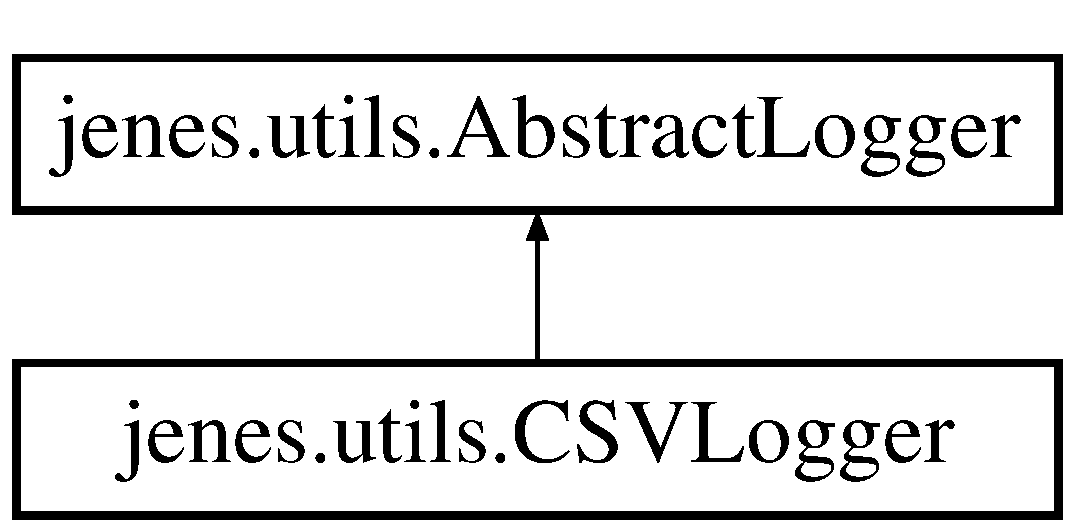
\includegraphics[height=2cm]{classjenes_1_1utils_1_1_c_s_v_logger}
\end{center}
\end{figure}
\subsection*{Public Member Functions}
\begin{CompactItemize}
\item 
\hyperlink{classjenes_1_1utils_1_1_c_s_v_logger_8cac9e217f74d86b4e26b025d8e1381c}{CSVLogger} (String\mbox{[}$\,$\mbox{]} \hyperlink{classjenes_1_1utils_1_1_abstract_logger_3a2030876857a0512fae7e0ad400c570}{schema})  throws FileNotFoundException 
\item 
\hyperlink{classjenes_1_1utils_1_1_c_s_v_logger_52ccc76492a8a16e018198bcfa702360}{CSVLogger} (String\mbox{[}$\,$\mbox{]} \hyperlink{classjenes_1_1utils_1_1_abstract_logger_3a2030876857a0512fae7e0ad400c570}{schema}, String filename)  throws FileNotFoundException 
\item 
\hyperlink{classjenes_1_1utils_1_1_c_s_v_logger_d6242d77cf75372bfbf55e9b0973bfb4}{CSVLogger} (String\mbox{[}$\,$\mbox{]} \hyperlink{classjenes_1_1utils_1_1_abstract_logger_3a2030876857a0512fae7e0ad400c570}{schema}, String filename, String separator)  throws FileNotFoundException 
\item 
\hyperlink{classjenes_1_1utils_1_1_c_s_v_logger_d39241223c9d49bfa34a21db4aa1f8b1}{CSVLogger} (String\mbox{[}$\,$\mbox{]} \hyperlink{classjenes_1_1utils_1_1_abstract_logger_3a2030876857a0512fae7e0ad400c570}{schema}, String filename, String separator, boolean header)  throws FileNotFoundException 
\item 
PrintWriter \hyperlink{classjenes_1_1utils_1_1_c_s_v_logger_00671f9154ae65398d676e6526fa08f2}{getOut} ()
\end{CompactItemize}
\subsection*{Protected Member Functions}
\begin{CompactItemize}
\item 
void \hyperlink{classjenes_1_1utils_1_1_c_s_v_logger_863bcfda3e93b023949a81e7f6d149e7}{store} ()
\item 
void \hyperlink{classjenes_1_1utils_1_1_c_s_v_logger_09a4f4fc362db6d4090d75642521ee65}{doSave} ()
\item 
void \hyperlink{classjenes_1_1utils_1_1_c_s_v_logger_c89f6fe5bd609fcc02ca7adf1407f279}{doClose} ()
\end{CompactItemize}


\subsection{Detailed Description}
This class defines a StatisticsLogger based on CSV (comma separated values) file. The logger has a schema, made of the fields the user means to record. If the schema is not specified, the logger use the set of keys making a record as schema. The default separator is tab, but a different separator can be specified at instantiation time. The default logfile is named log.csv and placed into the working directory. The logger can record or not the first line with the header made of the field names.

\begin{Desc}
\item[Version:]1.3 \end{Desc}
\begin{Desc}
\item[Since:]1.3 \end{Desc}


\subsection{Constructor \& Destructor Documentation}
\hypertarget{classjenes_1_1utils_1_1_c_s_v_logger_8cac9e217f74d86b4e26b025d8e1381c}{
\index{jenes::utils::CSVLogger@{jenes::utils::CSVLogger}!CSVLogger@{CSVLogger}}
\index{CSVLogger@{CSVLogger}!jenes::utils::CSVLogger@{jenes::utils::CSVLogger}}
\subsubsection[CSVLogger]{\setlength{\rightskip}{0pt plus 5cm}jenes.utils.CSVLogger.CSVLogger (String\mbox{[}$\,$\mbox{]} {\em schema})  throws FileNotFoundException }}
\label{classjenes_1_1utils_1_1_c_s_v_logger_8cac9e217f74d86b4e26b025d8e1381c}


Creates a logger with the specified schema, and log.csv as default filename, tab as default separator. The header is placed on the first line.

\begin{Desc}
\item[Parameters:]
\begin{description}
\item[{\em schema}]- the array making the schema of records \end{description}
\end{Desc}
\begin{Desc}
\item[Exceptions:]
\begin{description}
\item[{\em java.io.FileNotFoundException}]\end{description}
\end{Desc}
\hypertarget{classjenes_1_1utils_1_1_c_s_v_logger_52ccc76492a8a16e018198bcfa702360}{
\index{jenes::utils::CSVLogger@{jenes::utils::CSVLogger}!CSVLogger@{CSVLogger}}
\index{CSVLogger@{CSVLogger}!jenes::utils::CSVLogger@{jenes::utils::CSVLogger}}
\subsubsection[CSVLogger]{\setlength{\rightskip}{0pt plus 5cm}jenes.utils.CSVLogger.CSVLogger (String\mbox{[}$\,$\mbox{]} {\em schema}, \/  String {\em filename})  throws FileNotFoundException }}
\label{classjenes_1_1utils_1_1_c_s_v_logger_52ccc76492a8a16e018198bcfa702360}


Creates a logger with the specified schema and filename, tab as default separator. The header is placed on the first line.

\begin{Desc}
\item[Parameters:]
\begin{description}
\item[{\em schema}]- the array making the schema of records \item[{\em filename}]- the output filename \end{description}
\end{Desc}
\begin{Desc}
\item[Exceptions:]
\begin{description}
\item[{\em java.io.FileNotFoundException}]\end{description}
\end{Desc}
\hypertarget{classjenes_1_1utils_1_1_c_s_v_logger_d6242d77cf75372bfbf55e9b0973bfb4}{
\index{jenes::utils::CSVLogger@{jenes::utils::CSVLogger}!CSVLogger@{CSVLogger}}
\index{CSVLogger@{CSVLogger}!jenes::utils::CSVLogger@{jenes::utils::CSVLogger}}
\subsubsection[CSVLogger]{\setlength{\rightskip}{0pt plus 5cm}jenes.utils.CSVLogger.CSVLogger (String\mbox{[}$\,$\mbox{]} {\em schema}, \/  String {\em filename}, \/  String {\em separator})  throws FileNotFoundException }}
\label{classjenes_1_1utils_1_1_c_s_v_logger_d6242d77cf75372bfbf55e9b0973bfb4}


Creates a logger with the specified schema, filename and separator. The header is placed on the first line.

\begin{Desc}
\item[Parameters:]
\begin{description}
\item[{\em schema}]- the array making the schema of records \item[{\em filename}]- the output filename \item[{\em separator}]- the values separator \end{description}
\end{Desc}
\begin{Desc}
\item[Exceptions:]
\begin{description}
\item[{\em java.io.FileNotFoundException}]\end{description}
\end{Desc}
\hypertarget{classjenes_1_1utils_1_1_c_s_v_logger_d39241223c9d49bfa34a21db4aa1f8b1}{
\index{jenes::utils::CSVLogger@{jenes::utils::CSVLogger}!CSVLogger@{CSVLogger}}
\index{CSVLogger@{CSVLogger}!jenes::utils::CSVLogger@{jenes::utils::CSVLogger}}
\subsubsection[CSVLogger]{\setlength{\rightskip}{0pt plus 5cm}jenes.utils.CSVLogger.CSVLogger (String\mbox{[}$\,$\mbox{]} {\em schema}, \/  String {\em filename}, \/  String {\em separator}, \/  boolean {\em header})  throws FileNotFoundException }}
\label{classjenes_1_1utils_1_1_c_s_v_logger_d39241223c9d49bfa34a21db4aa1f8b1}


Creates a logger with the specified schema, filename and separator. The header is placed on the first line if required.

\begin{Desc}
\item[Parameters:]
\begin{description}
\item[{\em schema}]- the array making the schema of records \item[{\em filename}]- the output filename \item[{\em separator}]- the values separator \item[{\em header}]- the header is included if true, otherwise not. \end{description}
\end{Desc}
\begin{Desc}
\item[Exceptions:]
\begin{description}
\item[{\em java.io.FileNotFoundException}]\end{description}
\end{Desc}


\subsection{Member Function Documentation}
\hypertarget{classjenes_1_1utils_1_1_c_s_v_logger_00671f9154ae65398d676e6526fa08f2}{
\index{jenes::utils::CSVLogger@{jenes::utils::CSVLogger}!getOut@{getOut}}
\index{getOut@{getOut}!jenes::utils::CSVLogger@{jenes::utils::CSVLogger}}
\subsubsection[getOut]{\setlength{\rightskip}{0pt plus 5cm}PrintWriter jenes.utils.CSVLogger.getOut ()}}
\label{classjenes_1_1utils_1_1_c_s_v_logger_00671f9154ae65398d676e6526fa08f2}


Return the output stream used for logging.

\begin{Desc}
\item[Returns:]the log writer \end{Desc}
\hypertarget{classjenes_1_1utils_1_1_c_s_v_logger_863bcfda3e93b023949a81e7f6d149e7}{
\index{jenes::utils::CSVLogger@{jenes::utils::CSVLogger}!store@{store}}
\index{store@{store}!jenes::utils::CSVLogger@{jenes::utils::CSVLogger}}
\subsubsection[store]{\setlength{\rightskip}{0pt plus 5cm}void jenes.utils.CSVLogger.store ()\hspace{0.3cm}{\tt  \mbox{[}protected, virtual\mbox{]}}}}
\label{classjenes_1_1utils_1_1_c_s_v_logger_863bcfda3e93b023949a81e7f6d149e7}


Stores the current record. 

Implements \hyperlink{classjenes_1_1utils_1_1_abstract_logger_6acf83a83999e26ae4ed45cbf355111b}{jenes.utils.AbstractLogger}.\hypertarget{classjenes_1_1utils_1_1_c_s_v_logger_09a4f4fc362db6d4090d75642521ee65}{
\index{jenes::utils::CSVLogger@{jenes::utils::CSVLogger}!doSave@{doSave}}
\index{doSave@{doSave}!jenes::utils::CSVLogger@{jenes::utils::CSVLogger}}
\subsubsection[doSave]{\setlength{\rightskip}{0pt plus 5cm}void jenes.utils.CSVLogger.doSave ()\hspace{0.3cm}{\tt  \mbox{[}protected, virtual\mbox{]}}}}
\label{classjenes_1_1utils_1_1_c_s_v_logger_09a4f4fc362db6d4090d75642521ee65}


Saves cached records on media 

Implements \hyperlink{classjenes_1_1utils_1_1_abstract_logger_41fcd50b050c467fe1b413fc5b49c167}{jenes.utils.AbstractLogger}.\hypertarget{classjenes_1_1utils_1_1_c_s_v_logger_c89f6fe5bd609fcc02ca7adf1407f279}{
\index{jenes::utils::CSVLogger@{jenes::utils::CSVLogger}!doClose@{doClose}}
\index{doClose@{doClose}!jenes::utils::CSVLogger@{jenes::utils::CSVLogger}}
\subsubsection[doClose]{\setlength{\rightskip}{0pt plus 5cm}void jenes.utils.CSVLogger.doClose ()\hspace{0.3cm}{\tt  \mbox{[}protected, virtual\mbox{]}}}}
\label{classjenes_1_1utils_1_1_c_s_v_logger_c89f6fe5bd609fcc02ca7adf1407f279}


Closes the logger. Any further log is not allowed. 

Implements \hyperlink{classjenes_1_1utils_1_1_abstract_logger_5253672b3f3f81287db2fc604ca921a9}{jenes.utils.AbstractLogger}.

The documentation for this class was generated from the following file:\begin{CompactItemize}
\item 
src/jenes/utils/CSVLogger.java\end{CompactItemize}

\hypertarget{classjenes_1_1stage_1_1operator_1_1common_1_1_de_jong_crowder_3_01_t_01extends_01_chromosome_01_4}{
\section{jenes.stage.operator.common.DeJongCrowder$<$ T extends Chromosome $>$ Class Reference}
\label{classjenes_1_1stage_1_1operator_1_1common_1_1_de_jong_crowder_3_01_t_01extends_01_chromosome_01_4}\index{jenes::stage::operator::common::DeJongCrowder$<$ T extends Chromosome $>$@{jenes::stage::operator::common::DeJongCrowder$<$ T extends Chromosome $>$}}
}
Inherits jenes::stage::operator::Crowder$<$ T $>$.

\subsection*{Public Types}
\begin{CompactItemize}
\item 
enum \hyperlink{classjenes_1_1stage_1_1operator_1_1common_1_1_de_jong_crowder_3_01_t_01extends_01_chromosome_01_4_4c04a136973e222068a9b2bad6593645}{SelectionMethod} \{ \par
\textbf{ROULETTE}, 
\textbf{TOURNAMENT}, 
\textbf{ROULETTE}, 
\textbf{TOURNAMENT}, 
\par
\textbf{ROULETTE}, 
\textbf{TOURNAMENT}, 
\textbf{NONE}, 
\textbf{ROULETTE}, 
\par
\textbf{TOURNAMENT}, 
\textbf{ROULETTE}, 
\textbf{TOURNAMENT}
 \}
\item 
enum \hyperlink{classjenes_1_1stage_1_1operator_1_1common_1_1_de_jong_crowder_3_01_t_01extends_01_chromosome_01_4_cd306135cc2dd505a1a981b36f4696ea}{CrossoverMethod} \{ \par
\textbf{SINGLEPOINT}, 
\textbf{TWOPOINTS}, 
\textbf{SINGLEPOINT}, 
\textbf{TWOPOINTS}, 
\par
\textbf{SINGLEPOINT}, 
\textbf{TWOPOINTS}, 
\textbf{SINGLEPOINT}, 
\textbf{TWOPOINTS}
 \}
\item 
enum \hyperlink{classjenes_1_1stage_1_1operator_1_1common_1_1_de_jong_crowder_3_01_t_01extends_01_chromosome_01_4_8f83051fb5a66142aaec4b66fddfff5c}{MutationMethod} \{ \par
\textbf{NONE}, 
\textbf{SIMPLE}, 
\textbf{NONE}, 
\textbf{SIMPLE}, 
\par
\textbf{NONE}, 
\textbf{SIMPLE}
 \}
\end{CompactItemize}
\subsection*{Public Member Functions}
\begin{CompactItemize}
\item 
\hyperlink{classjenes_1_1stage_1_1operator_1_1common_1_1_de_jong_crowder_3_01_t_01extends_01_chromosome_01_4_3a856be20539434c822eecf5fc099657}{DeJongCrowder} (final int sr, final int cf)
\item 
\hyperlink{classjenes_1_1stage_1_1operator_1_1common_1_1_de_jong_crowder_3_01_t_01extends_01_chromosome_01_4_552f2f1d77a10c3ae9fb8c94924fb798}{DeJongCrowder} (final int sr, final int cf, final \hyperlink{classjenes_1_1stage_1_1operator_1_1common_1_1_de_jong_crowder_3_01_t_01extends_01_chromosome_01_4_4c04a136973e222068a9b2bad6593645}{SelectionMethod} selmethod)
\item 
\hyperlink{classjenes_1_1stage_1_1operator_1_1common_1_1_de_jong_crowder_3_01_t_01extends_01_chromosome_01_4_50f143494ddff28214ac72497b0de52a}{DeJongCrowder} (final int sr, final int cf, final \hyperlink{classjenes_1_1stage_1_1operator_1_1common_1_1_de_jong_crowder_3_01_t_01extends_01_chromosome_01_4_4c04a136973e222068a9b2bad6593645}{SelectionMethod} selmethod, final \hyperlink{classjenes_1_1stage_1_1operator_1_1common_1_1_de_jong_crowder_3_01_t_01extends_01_chromosome_01_4_cd306135cc2dd505a1a981b36f4696ea}{CrossoverMethod} crossmethod)
\item 
\hyperlink{classjenes_1_1stage_1_1operator_1_1common_1_1_de_jong_crowder_3_01_t_01extends_01_chromosome_01_4_31f097247f16221e2074ddc05d198349}{DeJongCrowder} (final int sr, final int cf, final \hyperlink{classjenes_1_1stage_1_1operator_1_1common_1_1_de_jong_crowder_3_01_t_01extends_01_chromosome_01_4_4c04a136973e222068a9b2bad6593645}{SelectionMethod} selmethod, final \hyperlink{classjenes_1_1stage_1_1operator_1_1common_1_1_de_jong_crowder_3_01_t_01extends_01_chromosome_01_4_cd306135cc2dd505a1a981b36f4696ea}{CrossoverMethod} crossmethod, final double crossover, final double mutation)
\item 
\hyperlink{classjenes_1_1stage_1_1operator_1_1common_1_1_de_jong_crowder_3_01_t_01extends_01_chromosome_01_4_97d47f09a66cf05e1cfb7630410de686}{DeJongCrowder} (final int sr, final int cf, final Selector$<$ T $>$ \hyperlink{classjenes_1_1stage_1_1operator_1_1common_1_1_de_jong_crowder_3_01_t_01extends_01_chromosome_01_4_6486b0225d345afd81b86dd04772d5ba}{selector}, final AbstractStage$<$ T $>$...stages)
\item 
final int \hyperlink{classjenes_1_1stage_1_1operator_1_1common_1_1_de_jong_crowder_3_01_t_01extends_01_chromosome_01_4_f34ed99b72eedd09864a9c447179b04e}{getCrowdingFactor} ()
\item 
void \hyperlink{classjenes_1_1stage_1_1operator_1_1common_1_1_de_jong_crowder_3_01_t_01extends_01_chromosome_01_4_3420256f796449f9f486e6dc85c52f0d}{setCrowdingFactor} (int cf)
\item 
final int \hyperlink{classjenes_1_1stage_1_1operator_1_1common_1_1_de_jong_crowder_3_01_t_01extends_01_chromosome_01_4_eae8a98bdc6da2261e6071ca62c5a066}{getSelectionRate} ()
\item 
void \hyperlink{classjenes_1_1stage_1_1operator_1_1common_1_1_de_jong_crowder_3_01_t_01extends_01_chromosome_01_4_4d1a71c514bb8ffaeba9a13434dc3635}{setSelectionRate} (int sr)
\item 
final Selector$<$ T $>$ \hyperlink{classjenes_1_1stage_1_1operator_1_1common_1_1_de_jong_crowder_3_01_t_01extends_01_chromosome_01_4_c407367e2e9ecad45bab4253ca920a1a}{getSelector} ()
\item 
void \hyperlink{classjenes_1_1stage_1_1operator_1_1common_1_1_de_jong_crowder_3_01_t_01extends_01_chromosome_01_4_880fdcaa7ccc39a3f5512b4bd58e74ad}{setSelector} (Selector$<$ T $>$ \hyperlink{classjenes_1_1stage_1_1operator_1_1common_1_1_de_jong_crowder_3_01_t_01extends_01_chromosome_01_4_6486b0225d345afd81b86dd04772d5ba}{selector})
\item 
\hypertarget{classjenes_1_1stage_1_1operator_1_1common_1_1_de_jong_crowder_3_01_t_01extends_01_chromosome_01_4_75bf0d077c6bff093600f1f4c333d3d1}{
void \textbf{setBiggerIsBetter} (boolean flag, boolean recursively)}
\label{classjenes_1_1stage_1_1operator_1_1common_1_1_de_jong_crowder_3_01_t_01extends_01_chromosome_01_4_75bf0d077c6bff093600f1f4c333d3d1}

\item 
void \hyperlink{classjenes_1_1stage_1_1operator_1_1common_1_1_de_jong_crowder_3_01_t_01extends_01_chromosome_01_4_856473a5ced464b1923545059c9f2e67}{setFitness} (Fitness fit, boolean recursively)
\end{CompactItemize}
\subsection*{Static Public Attributes}
\begin{CompactItemize}
\item 
static final \hyperlink{classjenes_1_1stage_1_1operator_1_1common_1_1_de_jong_crowder_3_01_t_01extends_01_chromosome_01_4_4c04a136973e222068a9b2bad6593645}{SelectionMethod} \hyperlink{classjenes_1_1stage_1_1operator_1_1common_1_1_de_jong_crowder_3_01_t_01extends_01_chromosome_01_4_21277e6e0728d4e83cc353337bc5f66d}{DEFAULT\_\-SELECTION\_\-METHOD} = SelectionMethod.TOURNAMENT
\item 
static final \hyperlink{classjenes_1_1stage_1_1operator_1_1common_1_1_de_jong_crowder_3_01_t_01extends_01_chromosome_01_4_cd306135cc2dd505a1a981b36f4696ea}{CrossoverMethod} \hyperlink{classjenes_1_1stage_1_1operator_1_1common_1_1_de_jong_crowder_3_01_t_01extends_01_chromosome_01_4_2798047916292a1449952a7274f9f26d}{DEFAULT\_\-CROSSOVER\_\-METHOD} = CrossoverMethod.SINGLEPOINT
\item 
static final double \hyperlink{classjenes_1_1stage_1_1operator_1_1common_1_1_de_jong_crowder_3_01_t_01extends_01_chromosome_01_4_522c94dff2a39743f6dfddec03a2ce47}{DEFAULT\_\-CROSSOVER\_\-PROBABILITY} = 0.8
\item 
static final double \hyperlink{classjenes_1_1stage_1_1operator_1_1common_1_1_de_jong_crowder_3_01_t_01extends_01_chromosome_01_4_19680564524e8d194044526740001c84}{DEFAULT\_\-MUTATION\_\-PROBABILITY} = 0.02
\item 
static final int \hyperlink{classjenes_1_1stage_1_1operator_1_1common_1_1_de_jong_crowder_3_01_t_01extends_01_chromosome_01_4_7e7afe01b26af0cdd28d392ab7866576}{DEFAULT\_\-CROWDING\_\-FACTOR} = 2
\end{CompactItemize}
\subsection*{Protected Member Functions}
\begin{CompactItemize}
\item 
\hypertarget{classjenes_1_1stage_1_1operator_1_1common_1_1_de_jong_crowder_3_01_t_01extends_01_chromosome_01_4_98f463e26bf3fd0fd703320007302594}{
void \textbf{preselect} (Population$<$ T $>$ in, Population$<$ T $>$ out)}
\label{classjenes_1_1stage_1_1operator_1_1common_1_1_de_jong_crowder_3_01_t_01extends_01_chromosome_01_4_98f463e26bf3fd0fd703320007302594}

\item 
\hypertarget{classjenes_1_1stage_1_1operator_1_1common_1_1_de_jong_crowder_3_01_t_01extends_01_chromosome_01_4_7d659276ad2103199080458c85acf59e}{
void \textbf{replace} (Population$<$ T $>$ initial, Population$<$ T $>$ preselected, Population$<$ T $>$ evolved, Population$<$ T $>$ out)}
\label{classjenes_1_1stage_1_1operator_1_1common_1_1_de_jong_crowder_3_01_t_01extends_01_chromosome_01_4_7d659276ad2103199080458c85acf59e}

\end{CompactItemize}
\subsection*{Protected Attributes}
\begin{CompactItemize}
\item 
Selector$<$ T $>$ \hyperlink{classjenes_1_1stage_1_1operator_1_1common_1_1_de_jong_crowder_3_01_t_01extends_01_chromosome_01_4_6486b0225d345afd81b86dd04772d5ba}{selector} = null
\item 
int \hyperlink{classjenes_1_1stage_1_1operator_1_1common_1_1_de_jong_crowder_3_01_t_01extends_01_chromosome_01_4_d876594787797e723425c09d74d0a05d}{crowdingFactor}
\end{CompactItemize}


\subsection{Detailed Description}
This class implements De Jong crowding.

\begin{Desc}
\item[Version:]2.0 \end{Desc}
\begin{Desc}
\item[Since:]2.0 \end{Desc}


\subsection{Member Enumeration Documentation}
\hypertarget{classjenes_1_1stage_1_1operator_1_1common_1_1_de_jong_crowder_3_01_t_01extends_01_chromosome_01_4_4c04a136973e222068a9b2bad6593645}{
\index{jenes::stage::operator::common::DeJongCrowder$<$ T extends Chromosome $>$@{jenes::stage::operator::common::DeJongCrowder$<$ T extends Chromosome $>$}!SelectionMethod@{SelectionMethod}}
\index{SelectionMethod@{SelectionMethod}!jenes::stage::operator::common::DeJongCrowder< T extends Chromosome >@{jenes::stage::operator::common::DeJongCrowder$<$ T extends Chromosome $>$}}
\subsubsection[SelectionMethod]{\setlength{\rightskip}{0pt plus 5cm}enum jenes::stage::operator::common::DeJongCrowder$<$ T extends Chromosome $>$::{\bf SelectionMethod}}}
\label{classjenes_1_1stage_1_1operator_1_1common_1_1_de_jong_crowder_3_01_t_01extends_01_chromosome_01_4_4c04a136973e222068a9b2bad6593645}


Provides the available selection methods \hypertarget{classjenes_1_1stage_1_1operator_1_1common_1_1_de_jong_crowder_3_01_t_01extends_01_chromosome_01_4_cd306135cc2dd505a1a981b36f4696ea}{
\index{jenes::stage::operator::common::DeJongCrowder$<$ T extends Chromosome $>$@{jenes::stage::operator::common::DeJongCrowder$<$ T extends Chromosome $>$}!CrossoverMethod@{CrossoverMethod}}
\index{CrossoverMethod@{CrossoverMethod}!jenes::stage::operator::common::DeJongCrowder< T extends Chromosome >@{jenes::stage::operator::common::DeJongCrowder$<$ T extends Chromosome $>$}}
\subsubsection[CrossoverMethod]{\setlength{\rightskip}{0pt plus 5cm}enum jenes::stage::operator::common::DeJongCrowder$<$ T extends Chromosome $>$::{\bf CrossoverMethod}}}
\label{classjenes_1_1stage_1_1operator_1_1common_1_1_de_jong_crowder_3_01_t_01extends_01_chromosome_01_4_cd306135cc2dd505a1a981b36f4696ea}


Provides the available crossover methods \hypertarget{classjenes_1_1stage_1_1operator_1_1common_1_1_de_jong_crowder_3_01_t_01extends_01_chromosome_01_4_8f83051fb5a66142aaec4b66fddfff5c}{
\index{jenes::stage::operator::common::DeJongCrowder$<$ T extends Chromosome $>$@{jenes::stage::operator::common::DeJongCrowder$<$ T extends Chromosome $>$}!MutationMethod@{MutationMethod}}
\index{MutationMethod@{MutationMethod}!jenes::stage::operator::common::DeJongCrowder< T extends Chromosome >@{jenes::stage::operator::common::DeJongCrowder$<$ T extends Chromosome $>$}}
\subsubsection[MutationMethod]{\setlength{\rightskip}{0pt plus 5cm}enum jenes::stage::operator::common::DeJongCrowder$<$ T extends Chromosome $>$::{\bf MutationMethod}}}
\label{classjenes_1_1stage_1_1operator_1_1common_1_1_de_jong_crowder_3_01_t_01extends_01_chromosome_01_4_8f83051fb5a66142aaec4b66fddfff5c}


Provides standard mutation methods 

\subsection{Constructor \& Destructor Documentation}
\hypertarget{classjenes_1_1stage_1_1operator_1_1common_1_1_de_jong_crowder_3_01_t_01extends_01_chromosome_01_4_3a856be20539434c822eecf5fc099657}{
\index{jenes::stage::operator::common::DeJongCrowder$<$ T extends Chromosome $>$@{jenes::stage::operator::common::DeJongCrowder$<$ T extends Chromosome $>$}!DeJongCrowder@{DeJongCrowder}}
\index{DeJongCrowder@{DeJongCrowder}!jenes::stage::operator::common::DeJongCrowder< T extends Chromosome >@{jenes::stage::operator::common::DeJongCrowder$<$ T extends Chromosome $>$}}
\subsubsection[DeJongCrowder]{\setlength{\rightskip}{0pt plus 5cm}jenes.stage.operator.common.DeJongCrowder$<$ T extends Chromosome $>$.DeJongCrowder (final int {\em sr}, \/  final int {\em cf})}}
\label{classjenes_1_1stage_1_1operator_1_1common_1_1_de_jong_crowder_3_01_t_01extends_01_chromosome_01_4_3a856be20539434c822eecf5fc099657}


Creates DeJongCrowder

\begin{Desc}
\item[Parameters:]
\begin{description}
\item[{\em sr}]selection rate \item[{\em cf}]crowding rate \end{description}
\end{Desc}
\hypertarget{classjenes_1_1stage_1_1operator_1_1common_1_1_de_jong_crowder_3_01_t_01extends_01_chromosome_01_4_552f2f1d77a10c3ae9fb8c94924fb798}{
\index{jenes::stage::operator::common::DeJongCrowder$<$ T extends Chromosome $>$@{jenes::stage::operator::common::DeJongCrowder$<$ T extends Chromosome $>$}!DeJongCrowder@{DeJongCrowder}}
\index{DeJongCrowder@{DeJongCrowder}!jenes::stage::operator::common::DeJongCrowder< T extends Chromosome >@{jenes::stage::operator::common::DeJongCrowder$<$ T extends Chromosome $>$}}
\subsubsection[DeJongCrowder]{\setlength{\rightskip}{0pt plus 5cm}jenes.stage.operator.common.DeJongCrowder$<$ T extends Chromosome $>$.DeJongCrowder (final int {\em sr}, \/  final int {\em cf}, \/  final {\bf SelectionMethod} {\em selmethod})}}
\label{classjenes_1_1stage_1_1operator_1_1common_1_1_de_jong_crowder_3_01_t_01extends_01_chromosome_01_4_552f2f1d77a10c3ae9fb8c94924fb798}


Creates DeJongCrowder

\begin{Desc}
\item[Parameters:]
\begin{description}
\item[{\em sr}]selection rate \item[{\em cf}]crowding rate \item[{\em selmethod}]selection method \end{description}
\end{Desc}
\hypertarget{classjenes_1_1stage_1_1operator_1_1common_1_1_de_jong_crowder_3_01_t_01extends_01_chromosome_01_4_50f143494ddff28214ac72497b0de52a}{
\index{jenes::stage::operator::common::DeJongCrowder$<$ T extends Chromosome $>$@{jenes::stage::operator::common::DeJongCrowder$<$ T extends Chromosome $>$}!DeJongCrowder@{DeJongCrowder}}
\index{DeJongCrowder@{DeJongCrowder}!jenes::stage::operator::common::DeJongCrowder< T extends Chromosome >@{jenes::stage::operator::common::DeJongCrowder$<$ T extends Chromosome $>$}}
\subsubsection[DeJongCrowder]{\setlength{\rightskip}{0pt plus 5cm}jenes.stage.operator.common.DeJongCrowder$<$ T extends Chromosome $>$.DeJongCrowder (final int {\em sr}, \/  final int {\em cf}, \/  final {\bf SelectionMethod} {\em selmethod}, \/  final {\bf CrossoverMethod} {\em crossmethod})}}
\label{classjenes_1_1stage_1_1operator_1_1common_1_1_de_jong_crowder_3_01_t_01extends_01_chromosome_01_4_50f143494ddff28214ac72497b0de52a}


Creates DeJongCrowder

\begin{Desc}
\item[Parameters:]
\begin{description}
\item[{\em sr}]selection rate \item[{\em cf}]crowding rate \item[{\em selmethod}]selection method \item[{\em crossmethod}]crossover method \item[{\em crossover}]crossover probability \end{description}
\end{Desc}
\hypertarget{classjenes_1_1stage_1_1operator_1_1common_1_1_de_jong_crowder_3_01_t_01extends_01_chromosome_01_4_31f097247f16221e2074ddc05d198349}{
\index{jenes::stage::operator::common::DeJongCrowder$<$ T extends Chromosome $>$@{jenes::stage::operator::common::DeJongCrowder$<$ T extends Chromosome $>$}!DeJongCrowder@{DeJongCrowder}}
\index{DeJongCrowder@{DeJongCrowder}!jenes::stage::operator::common::DeJongCrowder< T extends Chromosome >@{jenes::stage::operator::common::DeJongCrowder$<$ T extends Chromosome $>$}}
\subsubsection[DeJongCrowder]{\setlength{\rightskip}{0pt plus 5cm}jenes.stage.operator.common.DeJongCrowder$<$ T extends Chromosome $>$.DeJongCrowder (final int {\em sr}, \/  final int {\em cf}, \/  final {\bf SelectionMethod} {\em selmethod}, \/  final {\bf CrossoverMethod} {\em crossmethod}, \/  final double {\em crossover}, \/  final double {\em mutation})}}
\label{classjenes_1_1stage_1_1operator_1_1common_1_1_de_jong_crowder_3_01_t_01extends_01_chromosome_01_4_31f097247f16221e2074ddc05d198349}


Creates DeJongCrowder

\begin{Desc}
\item[Parameters:]
\begin{description}
\item[{\em sr}]selection rate \item[{\em cf}]crowding rate \item[{\em selmethod}]selection method \item[{\em crossmethod}]crossover method \item[{\em crossover}]crossover probability \item[{\em mutation}]mutation probability \end{description}
\end{Desc}
\hypertarget{classjenes_1_1stage_1_1operator_1_1common_1_1_de_jong_crowder_3_01_t_01extends_01_chromosome_01_4_97d47f09a66cf05e1cfb7630410de686}{
\index{jenes::stage::operator::common::DeJongCrowder$<$ T extends Chromosome $>$@{jenes::stage::operator::common::DeJongCrowder$<$ T extends Chromosome $>$}!DeJongCrowder@{DeJongCrowder}}
\index{DeJongCrowder@{DeJongCrowder}!jenes::stage::operator::common::DeJongCrowder< T extends Chromosome >@{jenes::stage::operator::common::DeJongCrowder$<$ T extends Chromosome $>$}}
\subsubsection[DeJongCrowder]{\setlength{\rightskip}{0pt plus 5cm}jenes.stage.operator.common.DeJongCrowder$<$ T extends Chromosome $>$.DeJongCrowder (final int {\em sr}, \/  final int {\em cf}, \/  final Selector$<$ T $>$ {\em selector}, \/  final AbstractStage$<$ T $>$... {\em stages})}}
\label{classjenes_1_1stage_1_1operator_1_1common_1_1_de_jong_crowder_3_01_t_01extends_01_chromosome_01_4_97d47f09a66cf05e1cfb7630410de686}


Creates DeJongCrowder

\begin{Desc}
\item[Parameters:]
\begin{description}
\item[{\em sr}]selection rate \item[{\em cf}]crowding rate \item[{\em selector}]selector \item[{\em stages}]the body stages \end{description}
\end{Desc}


\subsection{Member Function Documentation}
\hypertarget{classjenes_1_1stage_1_1operator_1_1common_1_1_de_jong_crowder_3_01_t_01extends_01_chromosome_01_4_f34ed99b72eedd09864a9c447179b04e}{
\index{jenes::stage::operator::common::DeJongCrowder$<$ T extends Chromosome $>$@{jenes::stage::operator::common::DeJongCrowder$<$ T extends Chromosome $>$}!getCrowdingFactor@{getCrowdingFactor}}
\index{getCrowdingFactor@{getCrowdingFactor}!jenes::stage::operator::common::DeJongCrowder< T extends Chromosome >@{jenes::stage::operator::common::DeJongCrowder$<$ T extends Chromosome $>$}}
\subsubsection[getCrowdingFactor]{\setlength{\rightskip}{0pt plus 5cm}final int jenes.stage.operator.common.DeJongCrowder$<$ T extends Chromosome $>$.getCrowdingFactor ()}}
\label{classjenes_1_1stage_1_1operator_1_1common_1_1_de_jong_crowder_3_01_t_01extends_01_chromosome_01_4_f34ed99b72eedd09864a9c447179b04e}


Returns the crowding factor

\begin{Desc}
\item[Returns:]\end{Desc}
\hypertarget{classjenes_1_1stage_1_1operator_1_1common_1_1_de_jong_crowder_3_01_t_01extends_01_chromosome_01_4_3420256f796449f9f486e6dc85c52f0d}{
\index{jenes::stage::operator::common::DeJongCrowder$<$ T extends Chromosome $>$@{jenes::stage::operator::common::DeJongCrowder$<$ T extends Chromosome $>$}!setCrowdingFactor@{setCrowdingFactor}}
\index{setCrowdingFactor@{setCrowdingFactor}!jenes::stage::operator::common::DeJongCrowder< T extends Chromosome >@{jenes::stage::operator::common::DeJongCrowder$<$ T extends Chromosome $>$}}
\subsubsection[setCrowdingFactor]{\setlength{\rightskip}{0pt plus 5cm}void jenes.stage.operator.common.DeJongCrowder$<$ T extends Chromosome $>$.setCrowdingFactor (int {\em cf})}}
\label{classjenes_1_1stage_1_1operator_1_1common_1_1_de_jong_crowder_3_01_t_01extends_01_chromosome_01_4_3420256f796449f9f486e6dc85c52f0d}


Sets the crouding factor

\begin{Desc}
\item[Parameters:]
\begin{description}
\item[{\em cf}]crowding factor \end{description}
\end{Desc}
\hypertarget{classjenes_1_1stage_1_1operator_1_1common_1_1_de_jong_crowder_3_01_t_01extends_01_chromosome_01_4_eae8a98bdc6da2261e6071ca62c5a066}{
\index{jenes::stage::operator::common::DeJongCrowder$<$ T extends Chromosome $>$@{jenes::stage::operator::common::DeJongCrowder$<$ T extends Chromosome $>$}!getSelectionRate@{getSelectionRate}}
\index{getSelectionRate@{getSelectionRate}!jenes::stage::operator::common::DeJongCrowder< T extends Chromosome >@{jenes::stage::operator::common::DeJongCrowder$<$ T extends Chromosome $>$}}
\subsubsection[getSelectionRate]{\setlength{\rightskip}{0pt plus 5cm}final int jenes.stage.operator.common.DeJongCrowder$<$ T extends Chromosome $>$.getSelectionRate ()}}
\label{classjenes_1_1stage_1_1operator_1_1common_1_1_de_jong_crowder_3_01_t_01extends_01_chromosome_01_4_eae8a98bdc6da2261e6071ca62c5a066}


Returns the selection rate

\begin{Desc}
\item[Returns:]\end{Desc}
\hypertarget{classjenes_1_1stage_1_1operator_1_1common_1_1_de_jong_crowder_3_01_t_01extends_01_chromosome_01_4_4d1a71c514bb8ffaeba9a13434dc3635}{
\index{jenes::stage::operator::common::DeJongCrowder$<$ T extends Chromosome $>$@{jenes::stage::operator::common::DeJongCrowder$<$ T extends Chromosome $>$}!setSelectionRate@{setSelectionRate}}
\index{setSelectionRate@{setSelectionRate}!jenes::stage::operator::common::DeJongCrowder< T extends Chromosome >@{jenes::stage::operator::common::DeJongCrowder$<$ T extends Chromosome $>$}}
\subsubsection[setSelectionRate]{\setlength{\rightskip}{0pt plus 5cm}void jenes.stage.operator.common.DeJongCrowder$<$ T extends Chromosome $>$.setSelectionRate (int {\em sr})}}
\label{classjenes_1_1stage_1_1operator_1_1common_1_1_de_jong_crowder_3_01_t_01extends_01_chromosome_01_4_4d1a71c514bb8ffaeba9a13434dc3635}


Sets the selection rate \begin{Desc}
\item[Parameters:]
\begin{description}
\item[{\em sr}]\end{description}
\end{Desc}
\hypertarget{classjenes_1_1stage_1_1operator_1_1common_1_1_de_jong_crowder_3_01_t_01extends_01_chromosome_01_4_c407367e2e9ecad45bab4253ca920a1a}{
\index{jenes::stage::operator::common::DeJongCrowder$<$ T extends Chromosome $>$@{jenes::stage::operator::common::DeJongCrowder$<$ T extends Chromosome $>$}!getSelector@{getSelector}}
\index{getSelector@{getSelector}!jenes::stage::operator::common::DeJongCrowder< T extends Chromosome >@{jenes::stage::operator::common::DeJongCrowder$<$ T extends Chromosome $>$}}
\subsubsection[getSelector]{\setlength{\rightskip}{0pt plus 5cm}final Selector$<$T$>$ jenes.stage.operator.common.DeJongCrowder$<$ T extends Chromosome $>$.getSelector ()}}
\label{classjenes_1_1stage_1_1operator_1_1common_1_1_de_jong_crowder_3_01_t_01extends_01_chromosome_01_4_c407367e2e9ecad45bab4253ca920a1a}


Returns the selector \begin{Desc}
\item[Returns:]\end{Desc}
\hypertarget{classjenes_1_1stage_1_1operator_1_1common_1_1_de_jong_crowder_3_01_t_01extends_01_chromosome_01_4_880fdcaa7ccc39a3f5512b4bd58e74ad}{
\index{jenes::stage::operator::common::DeJongCrowder$<$ T extends Chromosome $>$@{jenes::stage::operator::common::DeJongCrowder$<$ T extends Chromosome $>$}!setSelector@{setSelector}}
\index{setSelector@{setSelector}!jenes::stage::operator::common::DeJongCrowder< T extends Chromosome >@{jenes::stage::operator::common::DeJongCrowder$<$ T extends Chromosome $>$}}
\subsubsection[setSelector]{\setlength{\rightskip}{0pt plus 5cm}void jenes.stage.operator.common.DeJongCrowder$<$ T extends Chromosome $>$.setSelector (Selector$<$ T $>$ {\em selector})}}
\label{classjenes_1_1stage_1_1operator_1_1common_1_1_de_jong_crowder_3_01_t_01extends_01_chromosome_01_4_880fdcaa7ccc39a3f5512b4bd58e74ad}


Sets the selector \begin{Desc}
\item[Parameters:]
\begin{description}
\item[{\em selector}]\end{description}
\end{Desc}
\hypertarget{classjenes_1_1stage_1_1operator_1_1common_1_1_de_jong_crowder_3_01_t_01extends_01_chromosome_01_4_856473a5ced464b1923545059c9f2e67}{
\index{jenes::stage::operator::common::DeJongCrowder$<$ T extends Chromosome $>$@{jenes::stage::operator::common::DeJongCrowder$<$ T extends Chromosome $>$}!setFitness@{setFitness}}
\index{setFitness@{setFitness}!jenes::stage::operator::common::DeJongCrowder< T extends Chromosome >@{jenes::stage::operator::common::DeJongCrowder$<$ T extends Chromosome $>$}}
\subsubsection[setFitness]{\setlength{\rightskip}{0pt plus 5cm}void jenes.stage.operator.common.DeJongCrowder$<$ T extends Chromosome $>$.setFitness (Fitness {\em fit}, \/  boolean {\em recursively})}}
\label{classjenes_1_1stage_1_1operator_1_1common_1_1_de_jong_crowder_3_01_t_01extends_01_chromosome_01_4_856473a5ced464b1923545059c9f2e67}


XXX \begin{Desc}
\item[Parameters:]
\begin{description}
\item[{\em fit}]\item[{\em recursively}]\end{description}
\end{Desc}


\subsection{Member Data Documentation}
\hypertarget{classjenes_1_1stage_1_1operator_1_1common_1_1_de_jong_crowder_3_01_t_01extends_01_chromosome_01_4_21277e6e0728d4e83cc353337bc5f66d}{
\index{jenes::stage::operator::common::DeJongCrowder$<$ T extends Chromosome $>$@{jenes::stage::operator::common::DeJongCrowder$<$ T extends Chromosome $>$}!DEFAULT\_\-SELECTION\_\-METHOD@{DEFAULT\_\-SELECTION\_\-METHOD}}
\index{DEFAULT\_\-SELECTION\_\-METHOD@{DEFAULT\_\-SELECTION\_\-METHOD}!jenes::stage::operator::common::DeJongCrowder< T extends Chromosome >@{jenes::stage::operator::common::DeJongCrowder$<$ T extends Chromosome $>$}}
\subsubsection[DEFAULT\_\-SELECTION\_\-METHOD]{\setlength{\rightskip}{0pt plus 5cm}final {\bf SelectionMethod} jenes.stage.operator.common.DeJongCrowder$<$ T extends Chromosome $>$.{\bf DEFAULT\_\-SELECTION\_\-METHOD} = SelectionMethod.TOURNAMENT\hspace{0.3cm}{\tt  \mbox{[}static\mbox{]}}}}
\label{classjenes_1_1stage_1_1operator_1_1common_1_1_de_jong_crowder_3_01_t_01extends_01_chromosome_01_4_21277e6e0728d4e83cc353337bc5f66d}


The default selection method \hypertarget{classjenes_1_1stage_1_1operator_1_1common_1_1_de_jong_crowder_3_01_t_01extends_01_chromosome_01_4_2798047916292a1449952a7274f9f26d}{
\index{jenes::stage::operator::common::DeJongCrowder$<$ T extends Chromosome $>$@{jenes::stage::operator::common::DeJongCrowder$<$ T extends Chromosome $>$}!DEFAULT\_\-CROSSOVER\_\-METHOD@{DEFAULT\_\-CROSSOVER\_\-METHOD}}
\index{DEFAULT\_\-CROSSOVER\_\-METHOD@{DEFAULT\_\-CROSSOVER\_\-METHOD}!jenes::stage::operator::common::DeJongCrowder< T extends Chromosome >@{jenes::stage::operator::common::DeJongCrowder$<$ T extends Chromosome $>$}}
\subsubsection[DEFAULT\_\-CROSSOVER\_\-METHOD]{\setlength{\rightskip}{0pt plus 5cm}final {\bf CrossoverMethod} jenes.stage.operator.common.DeJongCrowder$<$ T extends Chromosome $>$.{\bf DEFAULT\_\-CROSSOVER\_\-METHOD} = CrossoverMethod.SINGLEPOINT\hspace{0.3cm}{\tt  \mbox{[}static\mbox{]}}}}
\label{classjenes_1_1stage_1_1operator_1_1common_1_1_de_jong_crowder_3_01_t_01extends_01_chromosome_01_4_2798047916292a1449952a7274f9f26d}


The default crossover method \hypertarget{classjenes_1_1stage_1_1operator_1_1common_1_1_de_jong_crowder_3_01_t_01extends_01_chromosome_01_4_522c94dff2a39743f6dfddec03a2ce47}{
\index{jenes::stage::operator::common::DeJongCrowder$<$ T extends Chromosome $>$@{jenes::stage::operator::common::DeJongCrowder$<$ T extends Chromosome $>$}!DEFAULT\_\-CROSSOVER\_\-PROBABILITY@{DEFAULT\_\-CROSSOVER\_\-PROBABILITY}}
\index{DEFAULT\_\-CROSSOVER\_\-PROBABILITY@{DEFAULT\_\-CROSSOVER\_\-PROBABILITY}!jenes::stage::operator::common::DeJongCrowder< T extends Chromosome >@{jenes::stage::operator::common::DeJongCrowder$<$ T extends Chromosome $>$}}
\subsubsection[DEFAULT\_\-CROSSOVER\_\-PROBABILITY]{\setlength{\rightskip}{0pt plus 5cm}final double jenes.stage.operator.common.DeJongCrowder$<$ T extends Chromosome $>$.{\bf DEFAULT\_\-CROSSOVER\_\-PROBABILITY} = 0.8\hspace{0.3cm}{\tt  \mbox{[}static\mbox{]}}}}
\label{classjenes_1_1stage_1_1operator_1_1common_1_1_de_jong_crowder_3_01_t_01extends_01_chromosome_01_4_522c94dff2a39743f6dfddec03a2ce47}


The default crossover probability \hypertarget{classjenes_1_1stage_1_1operator_1_1common_1_1_de_jong_crowder_3_01_t_01extends_01_chromosome_01_4_19680564524e8d194044526740001c84}{
\index{jenes::stage::operator::common::DeJongCrowder$<$ T extends Chromosome $>$@{jenes::stage::operator::common::DeJongCrowder$<$ T extends Chromosome $>$}!DEFAULT\_\-MUTATION\_\-PROBABILITY@{DEFAULT\_\-MUTATION\_\-PROBABILITY}}
\index{DEFAULT\_\-MUTATION\_\-PROBABILITY@{DEFAULT\_\-MUTATION\_\-PROBABILITY}!jenes::stage::operator::common::DeJongCrowder< T extends Chromosome >@{jenes::stage::operator::common::DeJongCrowder$<$ T extends Chromosome $>$}}
\subsubsection[DEFAULT\_\-MUTATION\_\-PROBABILITY]{\setlength{\rightskip}{0pt plus 5cm}final double jenes.stage.operator.common.DeJongCrowder$<$ T extends Chromosome $>$.{\bf DEFAULT\_\-MUTATION\_\-PROBABILITY} = 0.02\hspace{0.3cm}{\tt  \mbox{[}static\mbox{]}}}}
\label{classjenes_1_1stage_1_1operator_1_1common_1_1_de_jong_crowder_3_01_t_01extends_01_chromosome_01_4_19680564524e8d194044526740001c84}


The default mutation probability \hypertarget{classjenes_1_1stage_1_1operator_1_1common_1_1_de_jong_crowder_3_01_t_01extends_01_chromosome_01_4_7e7afe01b26af0cdd28d392ab7866576}{
\index{jenes::stage::operator::common::DeJongCrowder$<$ T extends Chromosome $>$@{jenes::stage::operator::common::DeJongCrowder$<$ T extends Chromosome $>$}!DEFAULT\_\-CROWDING\_\-FACTOR@{DEFAULT\_\-CROWDING\_\-FACTOR}}
\index{DEFAULT\_\-CROWDING\_\-FACTOR@{DEFAULT\_\-CROWDING\_\-FACTOR}!jenes::stage::operator::common::DeJongCrowder< T extends Chromosome >@{jenes::stage::operator::common::DeJongCrowder$<$ T extends Chromosome $>$}}
\subsubsection[DEFAULT\_\-CROWDING\_\-FACTOR]{\setlength{\rightskip}{0pt plus 5cm}final int jenes.stage.operator.common.DeJongCrowder$<$ T extends Chromosome $>$.{\bf DEFAULT\_\-CROWDING\_\-FACTOR} = 2\hspace{0.3cm}{\tt  \mbox{[}static\mbox{]}}}}
\label{classjenes_1_1stage_1_1operator_1_1common_1_1_de_jong_crowder_3_01_t_01extends_01_chromosome_01_4_7e7afe01b26af0cdd28d392ab7866576}


The default crowding selectionRate \hypertarget{classjenes_1_1stage_1_1operator_1_1common_1_1_de_jong_crowder_3_01_t_01extends_01_chromosome_01_4_6486b0225d345afd81b86dd04772d5ba}{
\index{jenes::stage::operator::common::DeJongCrowder$<$ T extends Chromosome $>$@{jenes::stage::operator::common::DeJongCrowder$<$ T extends Chromosome $>$}!selector@{selector}}
\index{selector@{selector}!jenes::stage::operator::common::DeJongCrowder< T extends Chromosome >@{jenes::stage::operator::common::DeJongCrowder$<$ T extends Chromosome $>$}}
\subsubsection[selector]{\setlength{\rightskip}{0pt plus 5cm}Selector$<$T$>$ jenes.stage.operator.common.DeJongCrowder$<$ T extends Chromosome $>$.{\bf selector} = null\hspace{0.3cm}{\tt  \mbox{[}protected\mbox{]}}}}
\label{classjenes_1_1stage_1_1operator_1_1common_1_1_de_jong_crowder_3_01_t_01extends_01_chromosome_01_4_6486b0225d345afd81b86dd04772d5ba}


The selctor used \hypertarget{classjenes_1_1stage_1_1operator_1_1common_1_1_de_jong_crowder_3_01_t_01extends_01_chromosome_01_4_d876594787797e723425c09d74d0a05d}{
\index{jenes::stage::operator::common::DeJongCrowder$<$ T extends Chromosome $>$@{jenes::stage::operator::common::DeJongCrowder$<$ T extends Chromosome $>$}!crowdingFactor@{crowdingFactor}}
\index{crowdingFactor@{crowdingFactor}!jenes::stage::operator::common::DeJongCrowder< T extends Chromosome >@{jenes::stage::operator::common::DeJongCrowder$<$ T extends Chromosome $>$}}
\subsubsection[crowdingFactor]{\setlength{\rightskip}{0pt plus 5cm}int jenes.stage.operator.common.DeJongCrowder$<$ T extends Chromosome $>$.{\bf crowdingFactor}\hspace{0.3cm}{\tt  \mbox{[}protected\mbox{]}}}}
\label{classjenes_1_1stage_1_1operator_1_1common_1_1_de_jong_crowder_3_01_t_01extends_01_chromosome_01_4_d876594787797e723425c09d74d0a05d}


The crowding factor 

The documentation for this class was generated from the following file:\begin{CompactItemize}
\item 
src/jenes/stage/operator/common/DeJongCrowder.java\end{CompactItemize}

\hypertarget{classjenes_1_1stage_1_1operator_1_1common_1_1_deterministic_crowder_3_01_t_01extends_01_chromosome_01_4}{
\section{jenes.stage.operator.common.DeterministicCrowder$<$ T extends Chromosome $>$ Class Reference}
\label{classjenes_1_1stage_1_1operator_1_1common_1_1_deterministic_crowder_3_01_t_01extends_01_chromosome_01_4}\index{jenes::stage::operator::common::DeterministicCrowder$<$ T extends Chromosome $>$@{jenes::stage::operator::common::DeterministicCrowder$<$ T extends Chromosome $>$}}
}
Inherits jenes::stage::operator::Crowder$<$ T $>$.

\subsection*{Public Types}
\begin{CompactItemize}
\item 
enum \hyperlink{classjenes_1_1stage_1_1operator_1_1common_1_1_deterministic_crowder_3_01_t_01extends_01_chromosome_01_4_f734ac23216aafb25e63014b0b676e67}{SelectionMethod} \{ \par
\textbf{ROULETTE}, 
\textbf{TOURNAMENT}, 
\textbf{ROULETTE}, 
\textbf{TOURNAMENT}, 
\par
\textbf{ROULETTE}, 
\textbf{TOURNAMENT}, 
\textbf{NONE}, 
\textbf{ROULETTE}, 
\par
\textbf{TOURNAMENT}, 
\textbf{ROULETTE}, 
\textbf{TOURNAMENT}
 \}
\item 
enum \hyperlink{classjenes_1_1stage_1_1operator_1_1common_1_1_deterministic_crowder_3_01_t_01extends_01_chromosome_01_4_e58e16af4a8087c42225aa099718231d}{CrossoverMethod} \{ \par
\textbf{SINGLEPOINT}, 
\textbf{TWOPOINTS}, 
\textbf{SINGLEPOINT}, 
\textbf{TWOPOINTS}, 
\par
\textbf{SINGLEPOINT}, 
\textbf{TWOPOINTS}, 
\textbf{SINGLEPOINT}, 
\textbf{TWOPOINTS}
 \}
\item 
enum \hyperlink{classjenes_1_1stage_1_1operator_1_1common_1_1_deterministic_crowder_3_01_t_01extends_01_chromosome_01_4_40d00705655302bc78c3e60aca4c43b5}{MutationMethod} \{ \par
\textbf{NONE}, 
\textbf{SIMPLE}, 
\textbf{NONE}, 
\textbf{SIMPLE}, 
\par
\textbf{NONE}, 
\textbf{SIMPLE}
 \}
\end{CompactItemize}
\subsection*{Public Member Functions}
\begin{CompactItemize}
\item 
\hyperlink{classjenes_1_1stage_1_1operator_1_1common_1_1_deterministic_crowder_3_01_t_01extends_01_chromosome_01_4_d52c0d6a4bc032c8c198bf05cc3acf6f}{DeterministicCrowder} ()
\item 
\hypertarget{classjenes_1_1stage_1_1operator_1_1common_1_1_deterministic_crowder_3_01_t_01extends_01_chromosome_01_4_e974a4b359a9a467dfa434dd47a27cf7}{
\textbf{DeterministicCrowder} (final \hyperlink{classjenes_1_1stage_1_1operator_1_1common_1_1_deterministic_crowder_3_01_t_01extends_01_chromosome_01_4_f734ac23216aafb25e63014b0b676e67}{SelectionMethod} selmethod, final \hyperlink{classjenes_1_1stage_1_1operator_1_1common_1_1_deterministic_crowder_3_01_t_01extends_01_chromosome_01_4_e58e16af4a8087c42225aa099718231d}{CrossoverMethod} crossmethod)}
\label{classjenes_1_1stage_1_1operator_1_1common_1_1_deterministic_crowder_3_01_t_01extends_01_chromosome_01_4_e974a4b359a9a467dfa434dd47a27cf7}

\item 
\hyperlink{classjenes_1_1stage_1_1operator_1_1common_1_1_deterministic_crowder_3_01_t_01extends_01_chromosome_01_4_a59e2a1dcdb2cd6cc7a70e344a77dd31}{DeterministicCrowder} (final \hyperlink{classjenes_1_1stage_1_1operator_1_1common_1_1_deterministic_crowder_3_01_t_01extends_01_chromosome_01_4_f734ac23216aafb25e63014b0b676e67}{SelectionMethod} selmethod, final \hyperlink{classjenes_1_1stage_1_1operator_1_1common_1_1_deterministic_crowder_3_01_t_01extends_01_chromosome_01_4_e58e16af4a8087c42225aa099718231d}{CrossoverMethod} crossmethod, final double cp, final double mp)
\item 
\hyperlink{classjenes_1_1stage_1_1operator_1_1common_1_1_deterministic_crowder_3_01_t_01extends_01_chromosome_01_4_d7eed64a7fe60239ba3289ebf6003e8c}{DeterministicCrowder} (final Selector$<$ T $>$ selector, final Crossover$<$ T $>$ crossover)
\item 
\hyperlink{classjenes_1_1stage_1_1operator_1_1common_1_1_deterministic_crowder_3_01_t_01extends_01_chromosome_01_4_6359043178a5e4d8922485528acbbcec}{DeterministicCrowder} (final Selector$<$ T $>$ selector, final Crossover$<$ T $>$ crossover, final Mutator$<$ T $>$ mutator)
\item 
\hypertarget{classjenes_1_1stage_1_1operator_1_1common_1_1_deterministic_crowder_3_01_t_01extends_01_chromosome_01_4_f7b258f528b701713808c16bca29ca66}{
void \textbf{setBiggerIsBetter} (boolean flag, boolean recursively)}
\label{classjenes_1_1stage_1_1operator_1_1common_1_1_deterministic_crowder_3_01_t_01extends_01_chromosome_01_4_f7b258f528b701713808c16bca29ca66}

\end{CompactItemize}
\subsection*{Static Public Attributes}
\begin{CompactItemize}
\item 
static final \hyperlink{classjenes_1_1stage_1_1operator_1_1common_1_1_deterministic_crowder_3_01_t_01extends_01_chromosome_01_4_f734ac23216aafb25e63014b0b676e67}{SelectionMethod} \hyperlink{classjenes_1_1stage_1_1operator_1_1common_1_1_deterministic_crowder_3_01_t_01extends_01_chromosome_01_4_5ca3f3abce0f3163383ed9158b154289}{DEFAULT\_\-SELECTION\_\-METHOD} = SelectionMethod.TOURNAMENT
\item 
static final \hyperlink{classjenes_1_1stage_1_1operator_1_1common_1_1_deterministic_crowder_3_01_t_01extends_01_chromosome_01_4_e58e16af4a8087c42225aa099718231d}{CrossoverMethod} \hyperlink{classjenes_1_1stage_1_1operator_1_1common_1_1_deterministic_crowder_3_01_t_01extends_01_chromosome_01_4_a09cba6e344d7681789f11213d6cccd0}{DEFAULT\_\-CROSSOVER\_\-METHOD} = CrossoverMethod.SINGLEPOINT
\item 
static final double \hyperlink{classjenes_1_1stage_1_1operator_1_1common_1_1_deterministic_crowder_3_01_t_01extends_01_chromosome_01_4_824ea51baffd4e4b2fb045d38b964321}{DEFAULT\_\-CROSSOVER\_\-PROBABILITY} = 0.8
\item 
static final double \hyperlink{classjenes_1_1stage_1_1operator_1_1common_1_1_deterministic_crowder_3_01_t_01extends_01_chromosome_01_4_5a4e77ddc158a661371ea5934cce2977}{DEFAULT\_\-MUTATION\_\-PROBABILITY} = 0.0
\end{CompactItemize}
\subsection*{Protected Member Functions}
\begin{CompactItemize}
\item 
\hypertarget{classjenes_1_1stage_1_1operator_1_1common_1_1_deterministic_crowder_3_01_t_01extends_01_chromosome_01_4_ee04796d9d0ad969443b30cc88a1b964}{
void \textbf{preselect} (Population$<$ T $>$ in, Population$<$ T $>$ out)}
\label{classjenes_1_1stage_1_1operator_1_1common_1_1_deterministic_crowder_3_01_t_01extends_01_chromosome_01_4_ee04796d9d0ad969443b30cc88a1b964}

\item 
\hypertarget{classjenes_1_1stage_1_1operator_1_1common_1_1_deterministic_crowder_3_01_t_01extends_01_chromosome_01_4_8d9591e3962f36f1f2f59be9395806b4}{
void \textbf{replace} (Population$<$ T $>$ initial, Population$<$ T $>$ preselected, Population$<$ T $>$ evolved, Population$<$ T $>$ out)}
\label{classjenes_1_1stage_1_1operator_1_1common_1_1_deterministic_crowder_3_01_t_01extends_01_chromosome_01_4_8d9591e3962f36f1f2f59be9395806b4}

\end{CompactItemize}


\subsection{Detailed Description}
This class implements the deterministic crowding.

\begin{Desc}
\item[Version:]2.0 \end{Desc}
\begin{Desc}
\item[Since:]2.0 \end{Desc}


\subsection{Member Enumeration Documentation}
\hypertarget{classjenes_1_1stage_1_1operator_1_1common_1_1_deterministic_crowder_3_01_t_01extends_01_chromosome_01_4_f734ac23216aafb25e63014b0b676e67}{
\index{jenes::stage::operator::common::DeterministicCrowder$<$ T extends Chromosome $>$@{jenes::stage::operator::common::DeterministicCrowder$<$ T extends Chromosome $>$}!SelectionMethod@{SelectionMethod}}
\index{SelectionMethod@{SelectionMethod}!jenes::stage::operator::common::DeterministicCrowder< T extends Chromosome >@{jenes::stage::operator::common::DeterministicCrowder$<$ T extends Chromosome $>$}}
\subsubsection[SelectionMethod]{\setlength{\rightskip}{0pt plus 5cm}enum jenes::stage::operator::common::DeterministicCrowder$<$ T extends Chromosome $>$::{\bf SelectionMethod}}}
\label{classjenes_1_1stage_1_1operator_1_1common_1_1_deterministic_crowder_3_01_t_01extends_01_chromosome_01_4_f734ac23216aafb25e63014b0b676e67}


Provides the available selection methods \hypertarget{classjenes_1_1stage_1_1operator_1_1common_1_1_deterministic_crowder_3_01_t_01extends_01_chromosome_01_4_e58e16af4a8087c42225aa099718231d}{
\index{jenes::stage::operator::common::DeterministicCrowder$<$ T extends Chromosome $>$@{jenes::stage::operator::common::DeterministicCrowder$<$ T extends Chromosome $>$}!CrossoverMethod@{CrossoverMethod}}
\index{CrossoverMethod@{CrossoverMethod}!jenes::stage::operator::common::DeterministicCrowder< T extends Chromosome >@{jenes::stage::operator::common::DeterministicCrowder$<$ T extends Chromosome $>$}}
\subsubsection[CrossoverMethod]{\setlength{\rightskip}{0pt plus 5cm}enum jenes::stage::operator::common::DeterministicCrowder$<$ T extends Chromosome $>$::{\bf CrossoverMethod}}}
\label{classjenes_1_1stage_1_1operator_1_1common_1_1_deterministic_crowder_3_01_t_01extends_01_chromosome_01_4_e58e16af4a8087c42225aa099718231d}


Provides the available crossover methods \hypertarget{classjenes_1_1stage_1_1operator_1_1common_1_1_deterministic_crowder_3_01_t_01extends_01_chromosome_01_4_40d00705655302bc78c3e60aca4c43b5}{
\index{jenes::stage::operator::common::DeterministicCrowder$<$ T extends Chromosome $>$@{jenes::stage::operator::common::DeterministicCrowder$<$ T extends Chromosome $>$}!MutationMethod@{MutationMethod}}
\index{MutationMethod@{MutationMethod}!jenes::stage::operator::common::DeterministicCrowder< T extends Chromosome >@{jenes::stage::operator::common::DeterministicCrowder$<$ T extends Chromosome $>$}}
\subsubsection[MutationMethod]{\setlength{\rightskip}{0pt plus 5cm}enum jenes::stage::operator::common::DeterministicCrowder$<$ T extends Chromosome $>$::{\bf MutationMethod}}}
\label{classjenes_1_1stage_1_1operator_1_1common_1_1_deterministic_crowder_3_01_t_01extends_01_chromosome_01_4_40d00705655302bc78c3e60aca4c43b5}


Provides standard mutation methods 

\subsection{Constructor \& Destructor Documentation}
\hypertarget{classjenes_1_1stage_1_1operator_1_1common_1_1_deterministic_crowder_3_01_t_01extends_01_chromosome_01_4_d52c0d6a4bc032c8c198bf05cc3acf6f}{
\index{jenes::stage::operator::common::DeterministicCrowder$<$ T extends Chromosome $>$@{jenes::stage::operator::common::DeterministicCrowder$<$ T extends Chromosome $>$}!DeterministicCrowder@{DeterministicCrowder}}
\index{DeterministicCrowder@{DeterministicCrowder}!jenes::stage::operator::common::DeterministicCrowder< T extends Chromosome >@{jenes::stage::operator::common::DeterministicCrowder$<$ T extends Chromosome $>$}}
\subsubsection[DeterministicCrowder]{\setlength{\rightskip}{0pt plus 5cm}jenes.stage.operator.common.DeterministicCrowder$<$ T extends Chromosome $>$.DeterministicCrowder ()}}
\label{classjenes_1_1stage_1_1operator_1_1common_1_1_deterministic_crowder_3_01_t_01extends_01_chromosome_01_4_d52c0d6a4bc032c8c198bf05cc3acf6f}


Creates a DeterministicCrowder with default options. \hypertarget{classjenes_1_1stage_1_1operator_1_1common_1_1_deterministic_crowder_3_01_t_01extends_01_chromosome_01_4_a59e2a1dcdb2cd6cc7a70e344a77dd31}{
\index{jenes::stage::operator::common::DeterministicCrowder$<$ T extends Chromosome $>$@{jenes::stage::operator::common::DeterministicCrowder$<$ T extends Chromosome $>$}!DeterministicCrowder@{DeterministicCrowder}}
\index{DeterministicCrowder@{DeterministicCrowder}!jenes::stage::operator::common::DeterministicCrowder< T extends Chromosome >@{jenes::stage::operator::common::DeterministicCrowder$<$ T extends Chromosome $>$}}
\subsubsection[DeterministicCrowder]{\setlength{\rightskip}{0pt plus 5cm}jenes.stage.operator.common.DeterministicCrowder$<$ T extends Chromosome $>$.DeterministicCrowder (final {\bf SelectionMethod} {\em selmethod}, \/  final {\bf CrossoverMethod} {\em crossmethod}, \/  final double {\em cp}, \/  final double {\em mp})}}
\label{classjenes_1_1stage_1_1operator_1_1common_1_1_deterministic_crowder_3_01_t_01extends_01_chromosome_01_4_a59e2a1dcdb2cd6cc7a70e344a77dd31}


Creates a DeterministicCrowder

\begin{Desc}
\item[Parameters:]
\begin{description}
\item[{\em selmethod}]selection method \item[{\em crossmethod}]crossover method \item[{\em cp}]croosover probability \item[{\em mp}]mutation probability \end{description}
\end{Desc}
\hypertarget{classjenes_1_1stage_1_1operator_1_1common_1_1_deterministic_crowder_3_01_t_01extends_01_chromosome_01_4_d7eed64a7fe60239ba3289ebf6003e8c}{
\index{jenes::stage::operator::common::DeterministicCrowder$<$ T extends Chromosome $>$@{jenes::stage::operator::common::DeterministicCrowder$<$ T extends Chromosome $>$}!DeterministicCrowder@{DeterministicCrowder}}
\index{DeterministicCrowder@{DeterministicCrowder}!jenes::stage::operator::common::DeterministicCrowder< T extends Chromosome >@{jenes::stage::operator::common::DeterministicCrowder$<$ T extends Chromosome $>$}}
\subsubsection[DeterministicCrowder]{\setlength{\rightskip}{0pt plus 5cm}jenes.stage.operator.common.DeterministicCrowder$<$ T extends Chromosome $>$.DeterministicCrowder (final Selector$<$ T $>$ {\em selector}, \/  final Crossover$<$ T $>$ {\em crossover})}}
\label{classjenes_1_1stage_1_1operator_1_1common_1_1_deterministic_crowder_3_01_t_01extends_01_chromosome_01_4_d7eed64a7fe60239ba3289ebf6003e8c}


Creates DeterministicCrowder providing selector and crossover operator

\begin{Desc}
\item[Parameters:]
\begin{description}
\item[{\em selector}]selection operator \item[{\em crossover}]crossover operator \end{description}
\end{Desc}
\hypertarget{classjenes_1_1stage_1_1operator_1_1common_1_1_deterministic_crowder_3_01_t_01extends_01_chromosome_01_4_6359043178a5e4d8922485528acbbcec}{
\index{jenes::stage::operator::common::DeterministicCrowder$<$ T extends Chromosome $>$@{jenes::stage::operator::common::DeterministicCrowder$<$ T extends Chromosome $>$}!DeterministicCrowder@{DeterministicCrowder}}
\index{DeterministicCrowder@{DeterministicCrowder}!jenes::stage::operator::common::DeterministicCrowder< T extends Chromosome >@{jenes::stage::operator::common::DeterministicCrowder$<$ T extends Chromosome $>$}}
\subsubsection[DeterministicCrowder]{\setlength{\rightskip}{0pt plus 5cm}jenes.stage.operator.common.DeterministicCrowder$<$ T extends Chromosome $>$.DeterministicCrowder (final Selector$<$ T $>$ {\em selector}, \/  final Crossover$<$ T $>$ {\em crossover}, \/  final Mutator$<$ T $>$ {\em mutator})}}
\label{classjenes_1_1stage_1_1operator_1_1common_1_1_deterministic_crowder_3_01_t_01extends_01_chromosome_01_4_6359043178a5e4d8922485528acbbcec}


Creates DeterministicCrowder providing selector, crossover and mutator operators

\begin{Desc}
\item[Parameters:]
\begin{description}
\item[{\em selector}]selection operator \item[{\em crossover}]crossover operator \item[{\em mutator}]mutation operator \end{description}
\end{Desc}


\subsection{Member Data Documentation}
\hypertarget{classjenes_1_1stage_1_1operator_1_1common_1_1_deterministic_crowder_3_01_t_01extends_01_chromosome_01_4_5ca3f3abce0f3163383ed9158b154289}{
\index{jenes::stage::operator::common::DeterministicCrowder$<$ T extends Chromosome $>$@{jenes::stage::operator::common::DeterministicCrowder$<$ T extends Chromosome $>$}!DEFAULT\_\-SELECTION\_\-METHOD@{DEFAULT\_\-SELECTION\_\-METHOD}}
\index{DEFAULT\_\-SELECTION\_\-METHOD@{DEFAULT\_\-SELECTION\_\-METHOD}!jenes::stage::operator::common::DeterministicCrowder< T extends Chromosome >@{jenes::stage::operator::common::DeterministicCrowder$<$ T extends Chromosome $>$}}
\subsubsection[DEFAULT\_\-SELECTION\_\-METHOD]{\setlength{\rightskip}{0pt plus 5cm}final {\bf SelectionMethod} jenes.stage.operator.common.DeterministicCrowder$<$ T extends Chromosome $>$.{\bf DEFAULT\_\-SELECTION\_\-METHOD} = SelectionMethod.TOURNAMENT\hspace{0.3cm}{\tt  \mbox{[}static\mbox{]}}}}
\label{classjenes_1_1stage_1_1operator_1_1common_1_1_deterministic_crowder_3_01_t_01extends_01_chromosome_01_4_5ca3f3abce0f3163383ed9158b154289}


The default selection method \hypertarget{classjenes_1_1stage_1_1operator_1_1common_1_1_deterministic_crowder_3_01_t_01extends_01_chromosome_01_4_a09cba6e344d7681789f11213d6cccd0}{
\index{jenes::stage::operator::common::DeterministicCrowder$<$ T extends Chromosome $>$@{jenes::stage::operator::common::DeterministicCrowder$<$ T extends Chromosome $>$}!DEFAULT\_\-CROSSOVER\_\-METHOD@{DEFAULT\_\-CROSSOVER\_\-METHOD}}
\index{DEFAULT\_\-CROSSOVER\_\-METHOD@{DEFAULT\_\-CROSSOVER\_\-METHOD}!jenes::stage::operator::common::DeterministicCrowder< T extends Chromosome >@{jenes::stage::operator::common::DeterministicCrowder$<$ T extends Chromosome $>$}}
\subsubsection[DEFAULT\_\-CROSSOVER\_\-METHOD]{\setlength{\rightskip}{0pt plus 5cm}final {\bf CrossoverMethod} jenes.stage.operator.common.DeterministicCrowder$<$ T extends Chromosome $>$.{\bf DEFAULT\_\-CROSSOVER\_\-METHOD} = CrossoverMethod.SINGLEPOINT\hspace{0.3cm}{\tt  \mbox{[}static\mbox{]}}}}
\label{classjenes_1_1stage_1_1operator_1_1common_1_1_deterministic_crowder_3_01_t_01extends_01_chromosome_01_4_a09cba6e344d7681789f11213d6cccd0}


The default crossover method \hypertarget{classjenes_1_1stage_1_1operator_1_1common_1_1_deterministic_crowder_3_01_t_01extends_01_chromosome_01_4_824ea51baffd4e4b2fb045d38b964321}{
\index{jenes::stage::operator::common::DeterministicCrowder$<$ T extends Chromosome $>$@{jenes::stage::operator::common::DeterministicCrowder$<$ T extends Chromosome $>$}!DEFAULT\_\-CROSSOVER\_\-PROBABILITY@{DEFAULT\_\-CROSSOVER\_\-PROBABILITY}}
\index{DEFAULT\_\-CROSSOVER\_\-PROBABILITY@{DEFAULT\_\-CROSSOVER\_\-PROBABILITY}!jenes::stage::operator::common::DeterministicCrowder< T extends Chromosome >@{jenes::stage::operator::common::DeterministicCrowder$<$ T extends Chromosome $>$}}
\subsubsection[DEFAULT\_\-CROSSOVER\_\-PROBABILITY]{\setlength{\rightskip}{0pt plus 5cm}final double jenes.stage.operator.common.DeterministicCrowder$<$ T extends Chromosome $>$.{\bf DEFAULT\_\-CROSSOVER\_\-PROBABILITY} = 0.8\hspace{0.3cm}{\tt  \mbox{[}static\mbox{]}}}}
\label{classjenes_1_1stage_1_1operator_1_1common_1_1_deterministic_crowder_3_01_t_01extends_01_chromosome_01_4_824ea51baffd4e4b2fb045d38b964321}


The default crossover probability \hypertarget{classjenes_1_1stage_1_1operator_1_1common_1_1_deterministic_crowder_3_01_t_01extends_01_chromosome_01_4_5a4e77ddc158a661371ea5934cce2977}{
\index{jenes::stage::operator::common::DeterministicCrowder$<$ T extends Chromosome $>$@{jenes::stage::operator::common::DeterministicCrowder$<$ T extends Chromosome $>$}!DEFAULT\_\-MUTATION\_\-PROBABILITY@{DEFAULT\_\-MUTATION\_\-PROBABILITY}}
\index{DEFAULT\_\-MUTATION\_\-PROBABILITY@{DEFAULT\_\-MUTATION\_\-PROBABILITY}!jenes::stage::operator::common::DeterministicCrowder< T extends Chromosome >@{jenes::stage::operator::common::DeterministicCrowder$<$ T extends Chromosome $>$}}
\subsubsection[DEFAULT\_\-MUTATION\_\-PROBABILITY]{\setlength{\rightskip}{0pt plus 5cm}final double jenes.stage.operator.common.DeterministicCrowder$<$ T extends Chromosome $>$.{\bf DEFAULT\_\-MUTATION\_\-PROBABILITY} = 0.0\hspace{0.3cm}{\tt  \mbox{[}static\mbox{]}}}}
\label{classjenes_1_1stage_1_1operator_1_1common_1_1_deterministic_crowder_3_01_t_01extends_01_chromosome_01_4_5a4e77ddc158a661371ea5934cce2977}


The default mutation probability 

The documentation for this class was generated from the following file:\begin{CompactItemize}
\item 
src/jenes/stage/operator/common/DeterministicCrowder.java\end{CompactItemize}

\hypertarget{classjenes_1_1stage_1_1_dispenser_3_01_t_01extends_01_chromosome_01_4}{
\section{jenes.stage.Dispenser$<$ T extends Chromosome $>$ Class Reference}
\label{classjenes_1_1stage_1_1_dispenser_3_01_t_01extends_01_chromosome_01_4}\index{jenes::stage::Dispenser$<$ T extends Chromosome $>$@{jenes::stage::Dispenser$<$ T extends Chromosome $>$}}
}
\subsection*{Public Member Functions}
\begin{CompactItemize}
\item 
\hyperlink{classjenes_1_1stage_1_1_dispenser_3_01_t_01extends_01_chromosome_01_4_8972dc3bcea956122cc623784a833bcf}{Dispenser} (int \hyperlink{classjenes_1_1stage_1_1_dispenser_3_01_t_01extends_01_chromosome_01_4_8f9bc0997e0536729db0c55bc9e240a5}{span})
\item 
int \hyperlink{classjenes_1_1stage_1_1_dispenser_3_01_t_01extends_01_chromosome_01_4_6ece937f3d7564424f6367e96e1b21c7}{span} ()
\item 
abstract void \hyperlink{classjenes_1_1stage_1_1_dispenser_3_01_t_01extends_01_chromosome_01_4_e9eb1e3be8a72e70e2bc75c53f31265b}{distribute} (Population$<$ T $>$ in, Population$<$ T $>$\mbox{[}$\,$\mbox{]} branches)
\item 
abstract void \hyperlink{classjenes_1_1stage_1_1_dispenser_3_01_t_01extends_01_chromosome_01_4_e35fcd8e2c1ecf6c9069107122b8a894}{mergePopulation} (Population$<$ T $>$\mbox{[}$\,$\mbox{]} branches, Population$<$ T $>$ out)
\end{CompactItemize}
\subsection*{Protected Attributes}
\begin{CompactItemize}
\item 
int \hyperlink{classjenes_1_1stage_1_1_dispenser_3_01_t_01extends_01_chromosome_01_4_8f9bc0997e0536729db0c55bc9e240a5}{span}
\end{CompactItemize}


\subsection{Detailed Description}
A Dispencer distributes a population between the branches of a parallel stage and merges the output of each branch in the output population of the parallel.\par
 \par
 The distribute method adds individual taken from the input population in one (or more) of the input population of the branches (see \hyperlink{}{distribute(Population, Population\mbox{[}$\,$\mbox{]})}). The number of branches is indicated by the span parameter passed to the constructor.\par
 \par
 For example, if span==2 can have\par
 

$<$blockquote$>$\small\begin{alltt}		
 	int count=0;	
 	for( Individual<T> i : in ) \{
 		int branch=count2;
 			branches[branch].add(i);
 	\}
 \end{alltt}
\normalsize 
$<$/blockquote$>$ The method \hyperlink{}{mergePopulation(Population\mbox{[}$\,$\mbox{]}, Population)} takes the output populations from the branches array and merges them in the output population according to some policy. A simple implementation is: 

$<$blockquote$>$\small\begin{alltt}
 	int count = 0;
 	for(Population<T>  branch : branches) \{
 		for(Individual<T> i : branch) \{
 			Individual<T> dest = out.getIndividual(count++);
 			// This check is necessary because out could have
 			// lesser elements than those resulting from branches
 			if( dest != null )
 				dest.setAs(i);
 			else\{
 				if(count<=out.size())
 					throw new IllegalStateException("out population can't contains null individual");
 				out.add(i.clone());
 			\}
 		\}
 	\}\end{alltt}
\normalsize 


\small\begin{alltt} 	// If out has more elements than the sum of elements
 	// resulting from branches, we remove the exceeding elements
 	int outSize=out.size();
 	for( int i = outSize-1; i >= count; --i )
 		out.remove(i);
 </blockquote>\end{alltt}
\normalsize 
 

\begin{Desc}
\item[Parameters:]
\begin{description}
\item[{\em $<$T$>$}]The class chromosomes flowing across the stage.\end{description}
\end{Desc}
\begin{Desc}
\item[Version:]1.2 \end{Desc}
\begin{Desc}
\item[Since:]1.0\end{Desc}
\begin{Desc}
\item[See also:]jenes.stage.Parallel \end{Desc}


\subsection{Constructor \& Destructor Documentation}
\hypertarget{classjenes_1_1stage_1_1_dispenser_3_01_t_01extends_01_chromosome_01_4_8972dc3bcea956122cc623784a833bcf}{
\index{jenes::stage::Dispenser$<$ T extends Chromosome $>$@{jenes::stage::Dispenser$<$ T extends Chromosome $>$}!Dispenser@{Dispenser}}
\index{Dispenser@{Dispenser}!jenes::stage::Dispenser< T extends Chromosome >@{jenes::stage::Dispenser$<$ T extends Chromosome $>$}}
\subsubsection[Dispenser]{\setlength{\rightskip}{0pt plus 5cm}jenes.stage.Dispenser$<$ T extends Chromosome $>$.Dispenser (int {\em span})}}
\label{classjenes_1_1stage_1_1_dispenser_3_01_t_01extends_01_chromosome_01_4_8972dc3bcea956122cc623784a833bcf}


Constructs a new dispencer with the specfied amplitude

\begin{Desc}
\item[Parameters:]
\begin{description}
\item[{\em span}]the dispencer amplitude \end{description}
\end{Desc}


\subsection{Member Function Documentation}
\hypertarget{classjenes_1_1stage_1_1_dispenser_3_01_t_01extends_01_chromosome_01_4_6ece937f3d7564424f6367e96e1b21c7}{
\index{jenes::stage::Dispenser$<$ T extends Chromosome $>$@{jenes::stage::Dispenser$<$ T extends Chromosome $>$}!span@{span}}
\index{span@{span}!jenes::stage::Dispenser< T extends Chromosome >@{jenes::stage::Dispenser$<$ T extends Chromosome $>$}}
\subsubsection[span]{\setlength{\rightskip}{0pt plus 5cm}int jenes.stage.Dispenser$<$ T extends Chromosome $>$.{\bf span} ()}}
\label{classjenes_1_1stage_1_1_dispenser_3_01_t_01extends_01_chromosome_01_4_6ece937f3d7564424f6367e96e1b21c7}


Returns the dispenser amplitude. 

\begin{Desc}
\item[Returns:]the dispenser amplitude \end{Desc}
\hypertarget{classjenes_1_1stage_1_1_dispenser_3_01_t_01extends_01_chromosome_01_4_e9eb1e3be8a72e70e2bc75c53f31265b}{
\index{jenes::stage::Dispenser$<$ T extends Chromosome $>$@{jenes::stage::Dispenser$<$ T extends Chromosome $>$}!distribute@{distribute}}
\index{distribute@{distribute}!jenes::stage::Dispenser< T extends Chromosome >@{jenes::stage::Dispenser$<$ T extends Chromosome $>$}}
\subsubsection[distribute]{\setlength{\rightskip}{0pt plus 5cm}abstract void jenes.stage.Dispenser$<$ T extends Chromosome $>$.distribute (Population$<$ T $>$ {\em in}, \/  Population$<$ T $>$\mbox{[}$\,$\mbox{]} {\em branches})\hspace{0.3cm}{\tt  \mbox{[}pure virtual\mbox{]}}}}
\label{classjenes_1_1stage_1_1_dispenser_3_01_t_01extends_01_chromosome_01_4_e9eb1e3be8a72e70e2bc75c53f31265b}


Distributes the specified population between those ones in the specified array. If some populations within inStagePop are not empty they will contain the initial individuals too at the end of distribute operation. 

\begin{Desc}
\item[Parameters:]
\begin{description}
\item[{\em in}]the population to be distributed \item[{\em branches}]the array of sub populations of the initial one \end{description}
\end{Desc}
\hypertarget{classjenes_1_1stage_1_1_dispenser_3_01_t_01extends_01_chromosome_01_4_e35fcd8e2c1ecf6c9069107122b8a894}{
\index{jenes::stage::Dispenser$<$ T extends Chromosome $>$@{jenes::stage::Dispenser$<$ T extends Chromosome $>$}!mergePopulation@{mergePopulation}}
\index{mergePopulation@{mergePopulation}!jenes::stage::Dispenser< T extends Chromosome >@{jenes::stage::Dispenser$<$ T extends Chromosome $>$}}
\subsubsection[mergePopulation]{\setlength{\rightskip}{0pt plus 5cm}abstract void jenes.stage.Dispenser$<$ T extends Chromosome $>$.mergePopulation (Population$<$ T $>$\mbox{[}$\,$\mbox{]} {\em branches}, \/  Population$<$ T $>$ {\em out})\hspace{0.3cm}{\tt  \mbox{[}pure virtual\mbox{]}}}}
\label{classjenes_1_1stage_1_1_dispenser_3_01_t_01extends_01_chromosome_01_4_e35fcd8e2c1ecf6c9069107122b8a894}


Merges the populations within the specified array in the specified one. If population is not empty it will contain the initial individuals too at the end of merge operation. 

\begin{Desc}
\item[Parameters:]
\begin{description}
\item[{\em out}]the final population \item[{\em branches}]the populations to be merged \end{description}
\end{Desc}


\subsection{Member Data Documentation}
\hypertarget{classjenes_1_1stage_1_1_dispenser_3_01_t_01extends_01_chromosome_01_4_8f9bc0997e0536729db0c55bc9e240a5}{
\index{jenes::stage::Dispenser$<$ T extends Chromosome $>$@{jenes::stage::Dispenser$<$ T extends Chromosome $>$}!span@{span}}
\index{span@{span}!jenes::stage::Dispenser< T extends Chromosome >@{jenes::stage::Dispenser$<$ T extends Chromosome $>$}}
\subsubsection[span]{\setlength{\rightskip}{0pt plus 5cm}int jenes.stage.Dispenser$<$ T extends Chromosome $>$.{\bf span}\hspace{0.3cm}{\tt  \mbox{[}protected\mbox{]}}}}
\label{classjenes_1_1stage_1_1_dispenser_3_01_t_01extends_01_chromosome_01_4_8f9bc0997e0536729db0c55bc9e240a5}


The dispencer amplitude, that is the number of populations where it will add individuals in the distribution method 

The documentation for this class was generated from the following file:\begin{CompactItemize}
\item 
src/jenes/stage/Dispenser.java\end{CompactItemize}

\hypertarget{classjenes_1_1tutorials_1_1problem5_1_1_double_allele_set}{
\section{jenes.tutorials.problem5.DoubleAlleleSet Class Reference}
\label{classjenes_1_1tutorials_1_1problem5_1_1_double_allele_set}\index{jenes::tutorials::problem5::DoubleAlleleSet@{jenes::tutorials::problem5::DoubleAlleleSet}}
}
Inherits jenes::chromosome::GenericAlleleSet$<$ Double $>$.

\subsection*{Public Member Functions}
\begin{CompactItemize}
\item 
\hypertarget{classjenes_1_1tutorials_1_1problem5_1_1_double_allele_set_3669132c61485f50aebe440a0602b2e5}{
\textbf{DoubleAlleleSet} (Set$<$ Double $>$ set)}
\label{classjenes_1_1tutorials_1_1problem5_1_1_double_allele_set_3669132c61485f50aebe440a0602b2e5}

\end{CompactItemize}
\subsection*{Static Public Member Functions}
\begin{CompactItemize}
\item 
static \hyperlink{classjenes_1_1tutorials_1_1problem5_1_1_double_allele_set}{DoubleAlleleSet} \hyperlink{classjenes_1_1tutorials_1_1problem5_1_1_double_allele_set_c831f648cab055cd70e3f1b47225529e}{createRandom} (int size, double lowerBound, double upperBound)
\item 
static \hyperlink{classjenes_1_1tutorials_1_1problem5_1_1_double_allele_set}{DoubleAlleleSet} \hyperlink{classjenes_1_1tutorials_1_1problem5_1_1_double_allele_set_75aa1cf3be84d1e3f5e50ecc0acc5b4b}{createUniform} (int size, int lowerBound, int upperBound)
\end{CompactItemize}


\subsection{Detailed Description}
Tutorial illustrating the use of object-oriented chromosomes, whose allele set can be defined by the user for each gene.

In this example the chromosomes are combinations of colors. We aim at finding the vector of colors closest to a given sequence.

This class defines an allele set made of doubles.

\begin{Desc}
\item[Version:]2.0 \end{Desc}
\begin{Desc}
\item[Since:]1.0 \end{Desc}


\subsection{Member Function Documentation}
\hypertarget{classjenes_1_1tutorials_1_1problem5_1_1_double_allele_set_c831f648cab055cd70e3f1b47225529e}{
\index{jenes::tutorials::problem5::DoubleAlleleSet@{jenes::tutorials::problem5::DoubleAlleleSet}!createRandom@{createRandom}}
\index{createRandom@{createRandom}!jenes::tutorials::problem5::DoubleAlleleSet@{jenes::tutorials::problem5::DoubleAlleleSet}}
\subsubsection[createRandom]{\setlength{\rightskip}{0pt plus 5cm}static {\bf DoubleAlleleSet} jenes.tutorials.problem5.DoubleAlleleSet.createRandom (int {\em size}, \/  double {\em lowerBound}, \/  double {\em upperBound})\hspace{0.3cm}{\tt  \mbox{[}static\mbox{]}}}}
\label{classjenes_1_1tutorials_1_1problem5_1_1_double_allele_set_c831f648cab055cd70e3f1b47225529e}


Builds a \hyperlink{classjenes_1_1tutorials_1_1problem5_1_1_double_allele_set}{DoubleAlleleSet} with random values within the range \mbox{[}lowerBound,upperBound\mbox{]} 

\begin{Desc}
\item[Parameters:]
\begin{description}
\item[{\em size}]the allala set cardinality \item[{\em lowerBound}]the min value to choose \item[{\em upperBound}]the max value to choose \end{description}
\end{Desc}
\begin{Desc}
\item[Returns:]a new \hyperlink{classjenes_1_1tutorials_1_1problem5_1_1_double_allele_set}{DoubleAlleleSet} \end{Desc}
\hypertarget{classjenes_1_1tutorials_1_1problem5_1_1_double_allele_set_75aa1cf3be84d1e3f5e50ecc0acc5b4b}{
\index{jenes::tutorials::problem5::DoubleAlleleSet@{jenes::tutorials::problem5::DoubleAlleleSet}!createUniform@{createUniform}}
\index{createUniform@{createUniform}!jenes::tutorials::problem5::DoubleAlleleSet@{jenes::tutorials::problem5::DoubleAlleleSet}}
\subsubsection[createUniform]{\setlength{\rightskip}{0pt plus 5cm}static {\bf DoubleAlleleSet} jenes.tutorials.problem5.DoubleAlleleSet.createUniform (int {\em size}, \/  int {\em lowerBound}, \/  int {\em upperBound})\hspace{0.3cm}{\tt  \mbox{[}static\mbox{]}}}}
\label{classjenes_1_1tutorials_1_1problem5_1_1_double_allele_set_75aa1cf3be84d1e3f5e50ecc0acc5b4b}


Builds a new \hyperlink{classjenes_1_1tutorials_1_1problem5_1_1_double_allele_set}{DoubleAlleleSet} with uniformly distributed values within the range \mbox{[}lowerBound,upperBound\mbox{]} 

\begin{Desc}
\item[Parameters:]
\begin{description}
\item[{\em size}]the allala set cardinality \item[{\em lowerBound}]the min value to choose \item[{\em upperBound}]the max value to choose \end{description}
\end{Desc}
\begin{Desc}
\item[Returns:]a new \hyperlink{classjenes_1_1tutorials_1_1problem5_1_1_double_allele_set}{DoubleAlleleSet} \end{Desc}


The documentation for this class was generated from the following file:\begin{CompactItemize}
\item 
src/jenes/tutorials/problem5/DoubleAlleleSet.java\end{CompactItemize}

\hypertarget{classjenes_1_1tutorials_1_1old_1_1problem5_1_1_double_allele_set}{
\section{jenes.tutorials.old.problem5.DoubleAlleleSet Class Reference}
\label{classjenes_1_1tutorials_1_1old_1_1problem5_1_1_double_allele_set}\index{jenes::tutorials::old::problem5::DoubleAlleleSet@{jenes::tutorials::old::problem5::DoubleAlleleSet}}
}
Inherits jenes::chromosome::GenericAlleleSet$<$ Double $>$.

\subsection*{Public Member Functions}
\begin{CompactItemize}
\item 
\hypertarget{classjenes_1_1tutorials_1_1old_1_1problem5_1_1_double_allele_set_16cde300bda10dc1ce20aa354514ad55}{
\textbf{DoubleAlleleSet} (Set$<$ Double $>$ set)}
\label{classjenes_1_1tutorials_1_1old_1_1problem5_1_1_double_allele_set_16cde300bda10dc1ce20aa354514ad55}

\end{CompactItemize}
\subsection*{Static Public Member Functions}
\begin{CompactItemize}
\item 
static \hyperlink{classjenes_1_1tutorials_1_1old_1_1problem5_1_1_double_allele_set}{DoubleAlleleSet} \hyperlink{classjenes_1_1tutorials_1_1old_1_1problem5_1_1_double_allele_set_b055f13f0aade5cd9bf21a42a6c00f67}{createRandom} (int size, double lowerBound, double upperBound)
\item 
static \hyperlink{classjenes_1_1tutorials_1_1old_1_1problem5_1_1_double_allele_set}{DoubleAlleleSet} \hyperlink{classjenes_1_1tutorials_1_1old_1_1problem5_1_1_double_allele_set_f442b73be0657db17a35d7fb376a98ed}{createUniform} (int size, int lowerBound, int upperBound)
\end{CompactItemize}


\subsection{Detailed Description}
Tutorial illustrating the use of object-oriented chromosomes, whose allele set can be defined by the user for each gene.

In this example the chromosomes are combinations of colors. We aim at finding the vector of colors closest to a given sequence.

This class defines an allele set made of doubles.

\begin{Desc}
\item[Version:]1.0 \end{Desc}
\begin{Desc}
\item[Since:]1.0 \end{Desc}


\subsection{Member Function Documentation}
\hypertarget{classjenes_1_1tutorials_1_1old_1_1problem5_1_1_double_allele_set_b055f13f0aade5cd9bf21a42a6c00f67}{
\index{jenes::tutorials::old::problem5::DoubleAlleleSet@{jenes::tutorials::old::problem5::DoubleAlleleSet}!createRandom@{createRandom}}
\index{createRandom@{createRandom}!jenes::tutorials::old::problem5::DoubleAlleleSet@{jenes::tutorials::old::problem5::DoubleAlleleSet}}
\subsubsection[createRandom]{\setlength{\rightskip}{0pt plus 5cm}static {\bf DoubleAlleleSet} jenes.tutorials.old.problem5.DoubleAlleleSet.createRandom (int {\em size}, \/  double {\em lowerBound}, \/  double {\em upperBound})\hspace{0.3cm}{\tt  \mbox{[}static\mbox{]}}}}
\label{classjenes_1_1tutorials_1_1old_1_1problem5_1_1_double_allele_set_b055f13f0aade5cd9bf21a42a6c00f67}


Builds a \hyperlink{classjenes_1_1tutorials_1_1old_1_1problem5_1_1_double_allele_set}{DoubleAlleleSet} with random values within the range \mbox{[}lowerBound,upperBound\mbox{]} 

\begin{Desc}
\item[Parameters:]
\begin{description}
\item[{\em size}]the allala set cardinality \item[{\em lowerBound}]the min value to choose \item[{\em upperBound}]the max value to choose \end{description}
\end{Desc}
\begin{Desc}
\item[Returns:]a new \hyperlink{classjenes_1_1tutorials_1_1old_1_1problem5_1_1_double_allele_set}{DoubleAlleleSet} \end{Desc}
\hypertarget{classjenes_1_1tutorials_1_1old_1_1problem5_1_1_double_allele_set_f442b73be0657db17a35d7fb376a98ed}{
\index{jenes::tutorials::old::problem5::DoubleAlleleSet@{jenes::tutorials::old::problem5::DoubleAlleleSet}!createUniform@{createUniform}}
\index{createUniform@{createUniform}!jenes::tutorials::old::problem5::DoubleAlleleSet@{jenes::tutorials::old::problem5::DoubleAlleleSet}}
\subsubsection[createUniform]{\setlength{\rightskip}{0pt plus 5cm}static {\bf DoubleAlleleSet} jenes.tutorials.old.problem5.DoubleAlleleSet.createUniform (int {\em size}, \/  int {\em lowerBound}, \/  int {\em upperBound})\hspace{0.3cm}{\tt  \mbox{[}static\mbox{]}}}}
\label{classjenes_1_1tutorials_1_1old_1_1problem5_1_1_double_allele_set_f442b73be0657db17a35d7fb376a98ed}


Builds a new \hyperlink{classjenes_1_1tutorials_1_1old_1_1problem5_1_1_double_allele_set}{DoubleAlleleSet} with uniformly distributed values within the range \mbox{[}lowerBound,upperBound\mbox{]} 

\begin{Desc}
\item[Parameters:]
\begin{description}
\item[{\em size}]the allala set cardinality \item[{\em lowerBound}]the min value to choose \item[{\em upperBound}]the max value to choose \end{description}
\end{Desc}
\begin{Desc}
\item[Returns:]a new \hyperlink{classjenes_1_1tutorials_1_1old_1_1problem5_1_1_double_allele_set}{DoubleAlleleSet} \end{Desc}


The documentation for this class was generated from the following file:\begin{CompactItemize}
\item 
src/jenes/tutorials/old/problem5/DoubleAlleleSet.java\end{CompactItemize}

\hypertarget{classjenes_1_1chromosome_1_1_double_chromosome}{
\section{jenes.chromosome.DoubleChromosome Class Reference}
\label{classjenes_1_1chromosome_1_1_double_chromosome}\index{jenes::chromosome::DoubleChromosome@{jenes::chromosome::DoubleChromosome}}
}
Inherits jenes::chromosome::Chromosome$<$ jenes::chromosome::DoubleChromosome $>$.

\subsection*{Public Member Functions}
\begin{CompactItemize}
\item 
\hyperlink{classjenes_1_1chromosome_1_1_double_chromosome_849079d41a2f10db681ba24de10d2619}{DoubleChromosome} (final \hyperlink{classjenes_1_1chromosome_1_1_double_chromosome}{DoubleChromosome} chromosome)
\item 
\hyperlink{classjenes_1_1chromosome_1_1_double_chromosome_7166da8f71e5b0cf37e751c053f6ff5f}{DoubleChromosome} (final int length, final double lowerBound, final double upperBound)
\item 
\hypertarget{classjenes_1_1chromosome_1_1_double_chromosome_82130d84dadedda332121b92f801d2e6}{
final void \textbf{setDefaultValueAt} (final int pos)}
\label{classjenes_1_1chromosome_1_1_double_chromosome_82130d84dadedda332121b92f801d2e6}

\item 
\hypertarget{classjenes_1_1chromosome_1_1_double_chromosome_c471f6b6cb7989e6b90c5e70e7b8a9a2}{
final \hyperlink{classjenes_1_1chromosome_1_1_double_chromosome}{DoubleChromosome} \textbf{clone} ()}
\label{classjenes_1_1chromosome_1_1_double_chromosome_c471f6b6cb7989e6b90c5e70e7b8a9a2}

\item 
\hypertarget{classjenes_1_1chromosome_1_1_double_chromosome_c34343c04259b0e3da8a7b2579cbd5fc}{
final void \textbf{swap} (final int pos1, final int pos2)}
\label{classjenes_1_1chromosome_1_1_double_chromosome_c34343c04259b0e3da8a7b2579cbd5fc}

\item 
\hypertarget{classjenes_1_1chromosome_1_1_double_chromosome_1ecf9f1d70333b8cbabdba918946cdfc}{
final void \textbf{randomize} ()}
\label{classjenes_1_1chromosome_1_1_double_chromosome_1ecf9f1d70333b8cbabdba918946cdfc}

\item 
\hypertarget{classjenes_1_1chromosome_1_1_double_chromosome_370f8d51fa8635eeadf925e2faf11991}{
final void \textbf{randomize} (final int pos)}
\label{classjenes_1_1chromosome_1_1_double_chromosome_370f8d51fa8635eeadf925e2faf11991}

\item 
\hypertarget{classjenes_1_1chromosome_1_1_double_chromosome_8d8eb8ce2b20abad8d462ae87a213e85}{
final void \textbf{leftShift} (final int from, int to)}
\label{classjenes_1_1chromosome_1_1_double_chromosome_8d8eb8ce2b20abad8d462ae87a213e85}

\item 
\hypertarget{classjenes_1_1chromosome_1_1_double_chromosome_e2c6d9bac13241a8338623c612d0f70b}{
final void \textbf{rightShift} (final int from, int to)}
\label{classjenes_1_1chromosome_1_1_double_chromosome_e2c6d9bac13241a8338623c612d0f70b}

\item 
\hypertarget{classjenes_1_1chromosome_1_1_double_chromosome_0938c891dcd64d56dcbfbc9136438b92}{
final int \textbf{length} ()}
\label{classjenes_1_1chromosome_1_1_double_chromosome_0938c891dcd64d56dcbfbc9136438b92}

\item 
\hypertarget{classjenes_1_1chromosome_1_1_double_chromosome_7479d1ee74934b04f478dcf8fad35464}{
final void \textbf{setAs} (final \hyperlink{classjenes_1_1chromosome_1_1_double_chromosome}{DoubleChromosome} chromosome)}
\label{classjenes_1_1chromosome_1_1_double_chromosome_7479d1ee74934b04f478dcf8fad35464}

\item 
\hypertarget{classjenes_1_1chromosome_1_1_double_chromosome_0461bfc35a8ca0c503ba0a4017005f89}{
final void \textbf{cross} (final \hyperlink{classjenes_1_1chromosome_1_1_double_chromosome}{DoubleChromosome} chromosome, final int from)}
\label{classjenes_1_1chromosome_1_1_double_chromosome_0461bfc35a8ca0c503ba0a4017005f89}

\item 
\hypertarget{classjenes_1_1chromosome_1_1_double_chromosome_caad58427cf1db8071fe2032755bbdce}{
final void \textbf{cross} (final \hyperlink{classjenes_1_1chromosome_1_1_double_chromosome}{DoubleChromosome} chromosome, final int from, final int to)}
\label{classjenes_1_1chromosome_1_1_double_chromosome_caad58427cf1db8071fe2032755bbdce}

\item 
final void \hyperlink{classjenes_1_1chromosome_1_1_double_chromosome_83b26a42b307ce1316523e262f044fdd}{average} (final \hyperlink{classjenes_1_1chromosome_1_1_double_chromosome}{DoubleChromosome} chromosome, double ratio)
\item 
final void \hyperlink{classjenes_1_1chromosome_1_1_double_chromosome_eebe5bd21dbc2e8dbbdc135d4d10a4cc}{owa} (final \hyperlink{classjenes_1_1chromosome_1_1_double_chromosome}{DoubleChromosome} chromosome, double ratio)
\item 
final double \hyperlink{classjenes_1_1chromosome_1_1_double_chromosome_cb68cbcac3e7859d4f380530355012c8}{getValue} (final int pos)
\item 
final double\mbox{[}$\,$\mbox{]} \hyperlink{classjenes_1_1chromosome_1_1_double_chromosome_3dea8e4aee9041437b101d1f74d10d1f}{getValues} ()
\item 
final double\mbox{[}$\,$\mbox{]} \hyperlink{classjenes_1_1chromosome_1_1_double_chromosome_0e7543f12f4ab7591f9b4687c44c801c}{getValues} (final double values\mbox{[}$\,$\mbox{]})
\item 
final void \hyperlink{classjenes_1_1chromosome_1_1_double_chromosome_b0f087d0d5ac5ac273c63c4e3af2efff}{setDefaultValue} (final double defaultValue)
\item 
final double \hyperlink{classjenes_1_1chromosome_1_1_double_chromosome_e129a0daa2e01593859f5b26c508d36b}{getDefaultValue} ()
\item 
final void \hyperlink{classjenes_1_1chromosome_1_1_double_chromosome_4581d7735d8ed661473b0e72ff19f956}{setValue} (final int pos, final double value)
\item 
final String \hyperlink{classjenes_1_1chromosome_1_1_double_chromosome_eaf1116586c3fac1fa8c1dad28b7f727}{toString} ()
\item 
final double \hyperlink{classjenes_1_1chromosome_1_1_double_chromosome_a45c550b4cb16cba001dd6c754a5d8bd}{getLowerBound} ()
\item 
final double \hyperlink{classjenes_1_1chromosome_1_1_double_chromosome_7f4fe0c4dd1645f02ebbb2633d6610c8}{getUpperBound} ()
\item 
final boolean \hyperlink{classjenes_1_1chromosome_1_1_double_chromosome_d661abf584ceb5195b6b248798709fc9}{equals} (final \hyperlink{classjenes_1_1chromosome_1_1_double_chromosome}{DoubleChromosome} chromosome)
\item 
\hypertarget{classjenes_1_1chromosome_1_1_double_chromosome_10f461747c9f99c02405626cf82aee46}{
void \textbf{difference} (final \hyperlink{classjenes_1_1chromosome_1_1_double_chromosome}{DoubleChromosome} chromosome, final double\mbox{[}$\,$\mbox{]} diff)}
\label{classjenes_1_1chromosome_1_1_double_chromosome_10f461747c9f99c02405626cf82aee46}

\item 
\hypertarget{classjenes_1_1chromosome_1_1_double_chromosome_101d1eb5ebc632c0c5d0a1c5b65daa90}{
Object\mbox{[}$\,$\mbox{]} \textbf{toArray} ()}
\label{classjenes_1_1chromosome_1_1_double_chromosome_101d1eb5ebc632c0c5d0a1c5b65daa90}

\end{CompactItemize}
\subsection*{Protected Attributes}
\begin{CompactItemize}
\item 
\hypertarget{classjenes_1_1chromosome_1_1_double_chromosome_0a987b7f1fa1c4cec652330ad77b6ba6}{
double\mbox{[}$\,$\mbox{]} \textbf{genes}}
\label{classjenes_1_1chromosome_1_1_double_chromosome_0a987b7f1fa1c4cec652330ad77b6ba6}

\item 
\hypertarget{classjenes_1_1chromosome_1_1_double_chromosome_56362107033b220e75d83b75ea91b74e}{
double \textbf{upperBound}}
\label{classjenes_1_1chromosome_1_1_double_chromosome_56362107033b220e75d83b75ea91b74e}

\item 
\hypertarget{classjenes_1_1chromosome_1_1_double_chromosome_f7c35ef9163f9ea35beb27b2c5985aa4}{
double \textbf{lowerBound}}
\label{classjenes_1_1chromosome_1_1_double_chromosome_f7c35ef9163f9ea35beb27b2c5985aa4}

\item 
\hypertarget{classjenes_1_1chromosome_1_1_double_chromosome_5c2d56f7d05b08c75013a7529ae46839}{
double \textbf{defaultValue} = 0}
\label{classjenes_1_1chromosome_1_1_double_chromosome_5c2d56f7d05b08c75013a7529ae46839}

\end{CompactItemize}


\subsection{Detailed Description}
A \hyperlink{classjenes_1_1chromosome_1_1_double_chromosome}{DoubleChromosome} is made of an array of double values. Each value is in the range \mbox{[}lowerBound,upperBound\mbox{[}. The lower bound is include included, the upper bound not. Both the bounds are specified ad the instantiation time. \hyperlink{classjenes_1_1chromosome_1_1_double_chromosome}{DoubleChromosome} is a fixed length chromosome class, thus number of genes is specified at instantiation time and cannot be modified after.

\begin{Desc}
\item[Version:]2.0 \end{Desc}
\begin{Desc}
\item[Since:]1.0 \end{Desc}


\subsection{Constructor \& Destructor Documentation}
\hypertarget{classjenes_1_1chromosome_1_1_double_chromosome_849079d41a2f10db681ba24de10d2619}{
\index{jenes::chromosome::DoubleChromosome@{jenes::chromosome::DoubleChromosome}!DoubleChromosome@{DoubleChromosome}}
\index{DoubleChromosome@{DoubleChromosome}!jenes::chromosome::DoubleChromosome@{jenes::chromosome::DoubleChromosome}}
\subsubsection[DoubleChromosome]{\setlength{\rightskip}{0pt plus 5cm}jenes.chromosome.DoubleChromosome.DoubleChromosome (final {\bf DoubleChromosome} {\em chromosome})}}
\label{classjenes_1_1chromosome_1_1_double_chromosome_849079d41a2f10db681ba24de10d2619}


Creates a new \hyperlink{classjenes_1_1chromosome_1_1_double_chromosome}{DoubleChromosome} as a copy of the specified chromosome 

\begin{Desc}
\item[Parameters:]
\begin{description}
\item[{\em chromosome}]the chromosome to be copied \end{description}
\end{Desc}
\hypertarget{classjenes_1_1chromosome_1_1_double_chromosome_7166da8f71e5b0cf37e751c053f6ff5f}{
\index{jenes::chromosome::DoubleChromosome@{jenes::chromosome::DoubleChromosome}!DoubleChromosome@{DoubleChromosome}}
\index{DoubleChromosome@{DoubleChromosome}!jenes::chromosome::DoubleChromosome@{jenes::chromosome::DoubleChromosome}}
\subsubsection[DoubleChromosome]{\setlength{\rightskip}{0pt plus 5cm}jenes.chromosome.DoubleChromosome.DoubleChromosome (final int {\em length}, \/  final double {\em lowerBound}, \/  final double {\em upperBound})}}
\label{classjenes_1_1chromosome_1_1_double_chromosome_7166da8f71e5b0cf37e751c053f6ff5f}


Creates a \hyperlink{classjenes_1_1chromosome_1_1_double_chromosome}{DoubleChromosome} with each allele in the range \mbox{[}lowerBound, upperBound\mbox{[} 

\begin{Desc}
\item[Parameters:]
\begin{description}
\item[{\em length}]the chromosome length \item[{\em lowerBound}]the lower bound \item[{\em upperBound}]the upper bound \end{description}
\end{Desc}


\subsection{Member Function Documentation}
\hypertarget{classjenes_1_1chromosome_1_1_double_chromosome_83b26a42b307ce1316523e262f044fdd}{
\index{jenes::chromosome::DoubleChromosome@{jenes::chromosome::DoubleChromosome}!average@{average}}
\index{average@{average}!jenes::chromosome::DoubleChromosome@{jenes::chromosome::DoubleChromosome}}
\subsubsection[average]{\setlength{\rightskip}{0pt plus 5cm}final void jenes.chromosome.DoubleChromosome.average (final {\bf DoubleChromosome} {\em chromosome}, \/  double {\em ratio})}}
\label{classjenes_1_1chromosome_1_1_double_chromosome_83b26a42b307ce1316523e262f044fdd}


Performs the weighted average between the genes in the two chromosomes. If ratio = 1, the chromosomes, do not change. If ratio = 0, chromosomes are swapped. The operation is performed until the end of shortest chromosome is reached.

\begin{Desc}
\item[Parameters:]
\begin{description}
\item[{\em chromosome}]- the chromosome to combine \item[{\em ratio}]- the coefficient used in the weighted average \end{description}
\end{Desc}
\hypertarget{classjenes_1_1chromosome_1_1_double_chromosome_eebe5bd21dbc2e8dbbdc135d4d10a4cc}{
\index{jenes::chromosome::DoubleChromosome@{jenes::chromosome::DoubleChromosome}!owa@{owa}}
\index{owa@{owa}!jenes::chromosome::DoubleChromosome@{jenes::chromosome::DoubleChromosome}}
\subsubsection[owa]{\setlength{\rightskip}{0pt plus 5cm}final void jenes.chromosome.DoubleChromosome.owa (final {\bf DoubleChromosome} {\em chromosome}, \/  double {\em ratio})}}
\label{classjenes_1_1chromosome_1_1_double_chromosome_eebe5bd21dbc2e8dbbdc135d4d10a4cc}


Performs the ordered weighted average (OWA) between the genes in the two chromosomes. If ratio = 1, the second chromosome holds the maximal values, the first the minimal. The opposite in case of ratio = 0. The operation is performed until the end of shortest chromosome is reached.

\begin{Desc}
\item[Parameters:]
\begin{description}
\item[{\em chromosome}]- the chromosome to combine \item[{\em ratio}]- the coefficient used in the weighted average \end{description}
\end{Desc}
\hypertarget{classjenes_1_1chromosome_1_1_double_chromosome_cb68cbcac3e7859d4f380530355012c8}{
\index{jenes::chromosome::DoubleChromosome@{jenes::chromosome::DoubleChromosome}!getValue@{getValue}}
\index{getValue@{getValue}!jenes::chromosome::DoubleChromosome@{jenes::chromosome::DoubleChromosome}}
\subsubsection[getValue]{\setlength{\rightskip}{0pt plus 5cm}final double jenes.chromosome.DoubleChromosome.getValue (final int {\em pos})}}
\label{classjenes_1_1chromosome_1_1_double_chromosome_cb68cbcac3e7859d4f380530355012c8}


Returns the double value at the specified position 

\begin{Desc}
\item[Parameters:]
\begin{description}
\item[{\em pos}]a position of this chromosome \end{description}
\end{Desc}
\begin{Desc}
\item[Returns:]the double value at the specified position \end{Desc}
\hypertarget{classjenes_1_1chromosome_1_1_double_chromosome_3dea8e4aee9041437b101d1f74d10d1f}{
\index{jenes::chromosome::DoubleChromosome@{jenes::chromosome::DoubleChromosome}!getValues@{getValues}}
\index{getValues@{getValues}!jenes::chromosome::DoubleChromosome@{jenes::chromosome::DoubleChromosome}}
\subsubsection[getValues]{\setlength{\rightskip}{0pt plus 5cm}final double \mbox{[}$\,$\mbox{]} jenes.chromosome.DoubleChromosome.getValues ()}}
\label{classjenes_1_1chromosome_1_1_double_chromosome_3dea8e4aee9041437b101d1f74d10d1f}


Returns the double values 

\begin{Desc}
\item[Returns:]values \end{Desc}
\hypertarget{classjenes_1_1chromosome_1_1_double_chromosome_0e7543f12f4ab7591f9b4687c44c801c}{
\index{jenes::chromosome::DoubleChromosome@{jenes::chromosome::DoubleChromosome}!getValues@{getValues}}
\index{getValues@{getValues}!jenes::chromosome::DoubleChromosome@{jenes::chromosome::DoubleChromosome}}
\subsubsection[getValues]{\setlength{\rightskip}{0pt plus 5cm}final double \mbox{[}$\,$\mbox{]} jenes.chromosome.DoubleChromosome.getValues (final double {\em values}\mbox{[}$\,$\mbox{]})}}
\label{classjenes_1_1chromosome_1_1_double_chromosome_0e7543f12f4ab7591f9b4687c44c801c}


Provides the gene values by the array passed as parameter and returning it on return. If the argument values is null, the array is first created. 

\begin{Desc}
\item[Parameters:]
\begin{description}
\item[{\em values}]the array to fill \end{description}
\end{Desc}
\begin{Desc}
\item[Returns:]the array of values \end{Desc}
\hypertarget{classjenes_1_1chromosome_1_1_double_chromosome_b0f087d0d5ac5ac273c63c4e3af2efff}{
\index{jenes::chromosome::DoubleChromosome@{jenes::chromosome::DoubleChromosome}!setDefaultValue@{setDefaultValue}}
\index{setDefaultValue@{setDefaultValue}!jenes::chromosome::DoubleChromosome@{jenes::chromosome::DoubleChromosome}}
\subsubsection[setDefaultValue]{\setlength{\rightskip}{0pt plus 5cm}final void jenes.chromosome.DoubleChromosome.setDefaultValue (final double {\em defaultValue})}}
\label{classjenes_1_1chromosome_1_1_double_chromosome_b0f087d0d5ac5ac273c63c4e3af2efff}


Sets the default value of this chromosome 

\begin{Desc}
\item[Parameters:]
\begin{description}
\item[{\em defaultValue}]the new default value to be used \end{description}
\end{Desc}
\hypertarget{classjenes_1_1chromosome_1_1_double_chromosome_e129a0daa2e01593859f5b26c508d36b}{
\index{jenes::chromosome::DoubleChromosome@{jenes::chromosome::DoubleChromosome}!getDefaultValue@{getDefaultValue}}
\index{getDefaultValue@{getDefaultValue}!jenes::chromosome::DoubleChromosome@{jenes::chromosome::DoubleChromosome}}
\subsubsection[getDefaultValue]{\setlength{\rightskip}{0pt plus 5cm}final double jenes.chromosome.DoubleChromosome.getDefaultValue ()}}
\label{classjenes_1_1chromosome_1_1_double_chromosome_e129a0daa2e01593859f5b26c508d36b}


Returns the default value of this chromosome 

\begin{Desc}
\item[Returns:]the double default value of this chromosome \end{Desc}
\hypertarget{classjenes_1_1chromosome_1_1_double_chromosome_4581d7735d8ed661473b0e72ff19f956}{
\index{jenes::chromosome::DoubleChromosome@{jenes::chromosome::DoubleChromosome}!setValue@{setValue}}
\index{setValue@{setValue}!jenes::chromosome::DoubleChromosome@{jenes::chromosome::DoubleChromosome}}
\subsubsection[setValue]{\setlength{\rightskip}{0pt plus 5cm}final void jenes.chromosome.DoubleChromosome.setValue (final int {\em pos}, \/  final double {\em value})}}
\label{classjenes_1_1chromosome_1_1_double_chromosome_4581d7735d8ed661473b0e72ff19f956}


Sets the specified value at the specified position 

\begin{Desc}
\item[Parameters:]
\begin{description}
\item[{\em pos}]the position to be modify \item[{\em value}]the value to be insert \end{description}
\end{Desc}
\hypertarget{classjenes_1_1chromosome_1_1_double_chromosome_eaf1116586c3fac1fa8c1dad28b7f727}{
\index{jenes::chromosome::DoubleChromosome@{jenes::chromosome::DoubleChromosome}!toString@{toString}}
\index{toString@{toString}!jenes::chromosome::DoubleChromosome@{jenes::chromosome::DoubleChromosome}}
\subsubsection[toString]{\setlength{\rightskip}{0pt plus 5cm}final String jenes.chromosome.DoubleChromosome.toString ()}}
\label{classjenes_1_1chromosome_1_1_double_chromosome_eaf1116586c3fac1fa8c1dad28b7f727}


Provides a textual chromosome representation \begin{Desc}
\item[Returns:]the textual chromosome representation \end{Desc}
\hypertarget{classjenes_1_1chromosome_1_1_double_chromosome_a45c550b4cb16cba001dd6c754a5d8bd}{
\index{jenes::chromosome::DoubleChromosome@{jenes::chromosome::DoubleChromosome}!getLowerBound@{getLowerBound}}
\index{getLowerBound@{getLowerBound}!jenes::chromosome::DoubleChromosome@{jenes::chromosome::DoubleChromosome}}
\subsubsection[getLowerBound]{\setlength{\rightskip}{0pt plus 5cm}final double jenes.chromosome.DoubleChromosome.getLowerBound ()}}
\label{classjenes_1_1chromosome_1_1_double_chromosome_a45c550b4cb16cba001dd6c754a5d8bd}


Returns the lower bound value for a gene of this chromosome

\begin{Desc}
\item[Returns:]the alleles lower bound \end{Desc}
\hypertarget{classjenes_1_1chromosome_1_1_double_chromosome_7f4fe0c4dd1645f02ebbb2633d6610c8}{
\index{jenes::chromosome::DoubleChromosome@{jenes::chromosome::DoubleChromosome}!getUpperBound@{getUpperBound}}
\index{getUpperBound@{getUpperBound}!jenes::chromosome::DoubleChromosome@{jenes::chromosome::DoubleChromosome}}
\subsubsection[getUpperBound]{\setlength{\rightskip}{0pt plus 5cm}final double jenes.chromosome.DoubleChromosome.getUpperBound ()}}
\label{classjenes_1_1chromosome_1_1_double_chromosome_7f4fe0c4dd1645f02ebbb2633d6610c8}


Returns the upper bound value for a gene of this chromosome

\begin{Desc}
\item[Returns:]the alleles upper bound \end{Desc}
\hypertarget{classjenes_1_1chromosome_1_1_double_chromosome_d661abf584ceb5195b6b248798709fc9}{
\index{jenes::chromosome::DoubleChromosome@{jenes::chromosome::DoubleChromosome}!equals@{equals}}
\index{equals@{equals}!jenes::chromosome::DoubleChromosome@{jenes::chromosome::DoubleChromosome}}
\subsubsection[equals]{\setlength{\rightskip}{0pt plus 5cm}final boolean jenes.chromosome.DoubleChromosome.equals (final {\bf DoubleChromosome} {\em chromosome})}}
\label{classjenes_1_1chromosome_1_1_double_chromosome_d661abf584ceb5195b6b248798709fc9}


Compares the chromosome with another.

\begin{Desc}
\item[Parameters:]
\begin{description}
\item[{\em chromosome}]the chromosome to compare to. \end{description}
\end{Desc}
\begin{Desc}
\item[Returns:]True, if the two chromosome are equal. \end{Desc}


The documentation for this class was generated from the following file:\begin{CompactItemize}
\item 
src/jenes/chromosome/DoubleChromosome.java\end{CompactItemize}

\hypertarget{classjenes_1_1tutorials_1_1problem4_1_1_entropy_fitness}{
\section{jenes.tutorials.problem4.EntropyFitness Class Reference}
\label{classjenes_1_1tutorials_1_1problem4_1_1_entropy_fitness}\index{jenes::tutorials::problem4::EntropyFitness@{jenes::tutorials::problem4::EntropyFitness}}
}
Inherits jenes::population::Fitness$<$ jenes::chromosome::DoubleChromosome $>$.

\subsection*{Public Member Functions}
\begin{CompactItemize}
\item 
\hypertarget{classjenes_1_1tutorials_1_1problem4_1_1_entropy_fitness_0e101073e060b84386ee2c10eb80a2f0}{
void \textbf{evaluate} (Individual$<$ \hyperlink{classjenes_1_1chromosome_1_1_double_chromosome}{DoubleChromosome} $>$ individual)}
\label{classjenes_1_1tutorials_1_1problem4_1_1_entropy_fitness_0e101073e060b84386ee2c10eb80a2f0}

\end{CompactItemize}
\subsection*{Static Public Attributes}
\begin{CompactItemize}
\item 
\hypertarget{classjenes_1_1tutorials_1_1problem4_1_1_entropy_fitness_015b775a1b2b1f1d5bc1eb82a560fe9a}{
static \hyperlink{classjenes_1_1tutorials_1_1problem4_1_1_entropy_fitness}{EntropyFitness} \textbf{MAX} = new \hyperlink{classjenes_1_1tutorials_1_1problem4_1_1_entropy_fitness}{EntropyFitness}(true)}
\label{classjenes_1_1tutorials_1_1problem4_1_1_entropy_fitness_015b775a1b2b1f1d5bc1eb82a560fe9a}

\item 
\hypertarget{classjenes_1_1tutorials_1_1problem4_1_1_entropy_fitness_b9c1db9f5da22216604985e98b6fc7e4}{
static \hyperlink{classjenes_1_1tutorials_1_1problem4_1_1_entropy_fitness}{EntropyFitness} \textbf{MIN} = new \hyperlink{classjenes_1_1tutorials_1_1problem4_1_1_entropy_fitness}{EntropyFitness}(false)}
\label{classjenes_1_1tutorials_1_1problem4_1_1_entropy_fitness_b9c1db9f5da22216604985e98b6fc7e4}

\end{CompactItemize}


\subsection{Detailed Description}
Tutorial showing how to set-up a minimization problem. The problem is to find a vector whose entroy, after normalization, is minimal.

\begin{Desc}
\item[Version:]2.0 \end{Desc}
\begin{Desc}
\item[Since:]1.0 \end{Desc}


The documentation for this class was generated from the following file:\begin{CompactItemize}
\item 
src/jenes/tutorials/problem4/EntropyFitness.java\end{CompactItemize}

\hypertarget{classjenes_1_1tutorials_1_1problem4_1_1_entropy_problem}{
\section{jenes.tutorials.problem4.EntropyProblem Class Reference}
\label{classjenes_1_1tutorials_1_1problem4_1_1_entropy_problem}\index{jenes::tutorials::problem4::EntropyProblem@{jenes::tutorials::problem4::EntropyProblem}}
}
\subsection*{Static Public Member Functions}
\begin{CompactItemize}
\item 
\hypertarget{classjenes_1_1tutorials_1_1problem4_1_1_entropy_problem_9b806aeb673e0324764205d27487524f}{
static void \textbf{main} (String\mbox{[}$\,$\mbox{]} args)}
\label{classjenes_1_1tutorials_1_1problem4_1_1_entropy_problem_9b806aeb673e0324764205d27487524f}

\end{CompactItemize}


\subsection{Detailed Description}
Tutorial showing how to set-up a minimization problem. The problem is to find a vector whose entroy, after normalization, is minimal.

\begin{Desc}
\item[Version:]2.0 \end{Desc}
\begin{Desc}
\item[Since:]1.0 \end{Desc}


The documentation for this class was generated from the following file:\begin{CompactItemize}
\item 
src/jenes/tutorials/problem4/EntropyProblem.java\end{CompactItemize}

\hypertarget{classjenes_1_1tutorials_1_1old_1_1problem4_1_1_entropy_problem}{
\section{jenes.tutorials.old.problem4.EntropyProblem Class Reference}
\label{classjenes_1_1tutorials_1_1old_1_1problem4_1_1_entropy_problem}\index{jenes::tutorials::old::problem4::EntropyProblem@{jenes::tutorials::old::problem4::EntropyProblem}}
}
\subsection*{Static Public Member Functions}
\begin{CompactItemize}
\item 
\hypertarget{classjenes_1_1tutorials_1_1old_1_1problem4_1_1_entropy_problem_0d51bbf6082f703157baaa168dd5f217}{
static void \textbf{main} (String\mbox{[}$\,$\mbox{]} args)}
\label{classjenes_1_1tutorials_1_1old_1_1problem4_1_1_entropy_problem_0d51bbf6082f703157baaa168dd5f217}

\end{CompactItemize}


\subsection{Detailed Description}
Tutorial showing how to set-up a minimization problem. The problem is to find a vector whose entroy, after normalization, is minimal.

\begin{Desc}
\item[Version:]1.0 \end{Desc}
\begin{Desc}
\item[Since:]1.0 \end{Desc}


The documentation for this class was generated from the following file:\begin{CompactItemize}
\item 
src/jenes/tutorials/old/problem4/EntropyProblem.java\end{CompactItemize}

\hypertarget{classjenes_1_1stage_1_1_evaluator_3_01_t_01extends_01_chromosome_01_4}{
\section{jenes.stage.Evaluator$<$ T extends Chromosome $>$ Class Reference}
\label{classjenes_1_1stage_1_1_evaluator_3_01_t_01extends_01_chromosome_01_4}\index{jenes::stage::Evaluator$<$ T extends Chromosome $>$@{jenes::stage::Evaluator$<$ T extends Chromosome $>$}}
}
Inherits jenes::stage::AbstractStage$<$ T $>$.

\subsection*{Public Member Functions}
\begin{CompactItemize}
\item 
\hyperlink{classjenes_1_1stage_1_1_evaluator_3_01_t_01extends_01_chromosome_01_4_fe7302209d1e39a0267bf4320d6d298d}{Evaluator} ()
\item 
\hyperlink{classjenes_1_1stage_1_1_evaluator_3_01_t_01extends_01_chromosome_01_4_d156e40a9579040474e6720f14c49919}{Evaluator} (boolean \hyperlink{classjenes_1_1stage_1_1_evaluator_3_01_t_01extends_01_chromosome_01_4_8ad6c1bcd555e06450a444d2d18b6b89}{force})
\item 
boolean \hyperlink{classjenes_1_1stage_1_1_evaluator_3_01_t_01extends_01_chromosome_01_4_617f44ce8de8d0e4bab8506e81038e76}{isForce} ()
\item 
void \hyperlink{classjenes_1_1stage_1_1_evaluator_3_01_t_01extends_01_chromosome_01_4_cd9d554678a83708eeb2d373def60e71}{setForce} (boolean \hyperlink{classjenes_1_1stage_1_1_evaluator_3_01_t_01extends_01_chromosome_01_4_8ad6c1bcd555e06450a444d2d18b6b89}{force})
\item 
void \hyperlink{classjenes_1_1stage_1_1_evaluator_3_01_t_01extends_01_chromosome_01_4_25aee75f7acf2406ca17526f588a8f15}{process} (Population$<$ T $>$ in, Population$<$ T $>$ out)  throws StageException 
\end{CompactItemize}
\subsection*{Protected Attributes}
\begin{CompactItemize}
\item 
boolean \hyperlink{classjenes_1_1stage_1_1_evaluator_3_01_t_01extends_01_chromosome_01_4_8ad6c1bcd555e06450a444d2d18b6b89}{force}
\end{CompactItemize}


\subsection{Detailed Description}
This stage performs a population evaluation. In general, individuals that have been alread avaluated, do not require be evaluated again. However, in order to provide full control to the user, the class has the property {\tt force} that if set, forces the evaluation of all individuals, despite the fact that the some individuals cold have been already evaluated. 

\begin{Desc}
\item[Parameters:]
\begin{description}
\item[{\em $<$T$>$}]The class chromosomes flowing across the stage.\end{description}
\end{Desc}
\begin{Desc}
\item[Version:]1.3 \end{Desc}
\begin{Desc}
\item[Since:]1.0 \end{Desc}


\subsection{Constructor \& Destructor Documentation}
\hypertarget{classjenes_1_1stage_1_1_evaluator_3_01_t_01extends_01_chromosome_01_4_fe7302209d1e39a0267bf4320d6d298d}{
\index{jenes::stage::Evaluator$<$ T extends Chromosome $>$@{jenes::stage::Evaluator$<$ T extends Chromosome $>$}!Evaluator@{Evaluator}}
\index{Evaluator@{Evaluator}!jenes::stage::Evaluator< T extends Chromosome >@{jenes::stage::Evaluator$<$ T extends Chromosome $>$}}
\subsubsection[Evaluator]{\setlength{\rightskip}{0pt plus 5cm}jenes.stage.Evaluator$<$ T extends Chromosome $>$.Evaluator ()}}
\label{classjenes_1_1stage_1_1_evaluator_3_01_t_01extends_01_chromosome_01_4_fe7302209d1e39a0267bf4320d6d298d}


Creates a new Evaluator instance. By default $<$colde$>$force is false. \hypertarget{classjenes_1_1stage_1_1_evaluator_3_01_t_01extends_01_chromosome_01_4_d156e40a9579040474e6720f14c49919}{
\index{jenes::stage::Evaluator$<$ T extends Chromosome $>$@{jenes::stage::Evaluator$<$ T extends Chromosome $>$}!Evaluator@{Evaluator}}
\index{Evaluator@{Evaluator}!jenes::stage::Evaluator< T extends Chromosome >@{jenes::stage::Evaluator$<$ T extends Chromosome $>$}}
\subsubsection[Evaluator]{\setlength{\rightskip}{0pt plus 5cm}jenes.stage.Evaluator$<$ T extends Chromosome $>$.Evaluator (boolean {\em force})}}
\label{classjenes_1_1stage_1_1_evaluator_3_01_t_01extends_01_chromosome_01_4_d156e40a9579040474e6720f14c49919}


Creates a new Evaluator instance, specifying the value of $<$colde$>$force.

\begin{Desc}
\item[Parameters:]
\begin{description}
\item[{\em force}]- if true, all individuals are forced to be evaluated in any case. \end{description}
\end{Desc}


\subsection{Member Function Documentation}
\hypertarget{classjenes_1_1stage_1_1_evaluator_3_01_t_01extends_01_chromosome_01_4_617f44ce8de8d0e4bab8506e81038e76}{
\index{jenes::stage::Evaluator$<$ T extends Chromosome $>$@{jenes::stage::Evaluator$<$ T extends Chromosome $>$}!isForce@{isForce}}
\index{isForce@{isForce}!jenes::stage::Evaluator< T extends Chromosome >@{jenes::stage::Evaluator$<$ T extends Chromosome $>$}}
\subsubsection[isForce]{\setlength{\rightskip}{0pt plus 5cm}boolean jenes.stage.Evaluator$<$ T extends Chromosome $>$.isForce ()}}
\label{classjenes_1_1stage_1_1_evaluator_3_01_t_01extends_01_chromosome_01_4_617f44ce8de8d0e4bab8506e81038e76}


Returns the current value of {\tt force}. By default this value is false. \begin{Desc}
\item[Returns:]the value of {\tt force}. \end{Desc}
\hypertarget{classjenes_1_1stage_1_1_evaluator_3_01_t_01extends_01_chromosome_01_4_cd9d554678a83708eeb2d373def60e71}{
\index{jenes::stage::Evaluator$<$ T extends Chromosome $>$@{jenes::stage::Evaluator$<$ T extends Chromosome $>$}!setForce@{setForce}}
\index{setForce@{setForce}!jenes::stage::Evaluator< T extends Chromosome >@{jenes::stage::Evaluator$<$ T extends Chromosome $>$}}
\subsubsection[setForce]{\setlength{\rightskip}{0pt plus 5cm}void jenes.stage.Evaluator$<$ T extends Chromosome $>$.setForce (boolean {\em force})}}
\label{classjenes_1_1stage_1_1_evaluator_3_01_t_01extends_01_chromosome_01_4_cd9d554678a83708eeb2d373def60e71}


Sets the value of {\tt force}. \begin{Desc}
\item[Parameters:]
\begin{description}
\item[{\em force}]- if true, all individuals are forced to be evaluated in any case. \end{description}
\end{Desc}
\hypertarget{classjenes_1_1stage_1_1_evaluator_3_01_t_01extends_01_chromosome_01_4_25aee75f7acf2406ca17526f588a8f15}{
\index{jenes::stage::Evaluator$<$ T extends Chromosome $>$@{jenes::stage::Evaluator$<$ T extends Chromosome $>$}!process@{process}}
\index{process@{process}!jenes::stage::Evaluator< T extends Chromosome >@{jenes::stage::Evaluator$<$ T extends Chromosome $>$}}
\subsubsection[process]{\setlength{\rightskip}{0pt plus 5cm}void jenes.stage.Evaluator$<$ T extends Chromosome $>$.process (Population$<$ T $>$ {\em in}, \/  Population$<$ T $>$ {\em out})  throws {\bf StageException} }}
\label{classjenes_1_1stage_1_1_evaluator_3_01_t_01extends_01_chromosome_01_4_25aee75f7acf2406ca17526f588a8f15}


Performs an evaluation of input population. \begin{Desc}
\item[Parameters:]
\begin{description}
\item[{\em in}]- the input population. \item[{\em out}]- equals the input population \end{description}
\end{Desc}
\begin{Desc}
\item[Exceptions:]
\begin{description}
\item[{\em \hyperlink{classjenes_1_1stage_1_1_stage_exception}{StageException}}]\end{description}
\end{Desc}


\subsection{Member Data Documentation}
\hypertarget{classjenes_1_1stage_1_1_evaluator_3_01_t_01extends_01_chromosome_01_4_8ad6c1bcd555e06450a444d2d18b6b89}{
\index{jenes::stage::Evaluator$<$ T extends Chromosome $>$@{jenes::stage::Evaluator$<$ T extends Chromosome $>$}!force@{force}}
\index{force@{force}!jenes::stage::Evaluator< T extends Chromosome >@{jenes::stage::Evaluator$<$ T extends Chromosome $>$}}
\subsubsection[force]{\setlength{\rightskip}{0pt plus 5cm}boolean jenes.stage.Evaluator$<$ T extends Chromosome $>$.{\bf force}\hspace{0.3cm}{\tt  \mbox{[}protected\mbox{]}}}}
\label{classjenes_1_1stage_1_1_evaluator_3_01_t_01extends_01_chromosome_01_4_8ad6c1bcd555e06450a444d2d18b6b89}


The property controlling if evaluation should be extened also to individuals already evaluated. 

The documentation for this class was generated from the following file:\begin{CompactItemize}
\item 
src/jenes/stage/Evaluator.java\end{CompactItemize}

\hypertarget{classjenes_1_1stage_1_1_exclusive_dispenser_3_01_t_01extends_01_chromosome_01_4}{
\section{jenes.stage.ExclusiveDispenser$<$ T extends Chromosome $>$ Class Reference}
\label{classjenes_1_1stage_1_1_exclusive_dispenser_3_01_t_01extends_01_chromosome_01_4}\index{jenes::stage::ExclusiveDispenser$<$ T extends Chromosome $>$@{jenes::stage::ExclusiveDispenser$<$ T extends Chromosome $>$}}
}
\subsection*{Public Member Functions}
\begin{CompactItemize}
\item 
\hyperlink{classjenes_1_1stage_1_1_exclusive_dispenser_3_01_t_01extends_01_chromosome_01_4_f8fba035b8567ce8d509fbc7601b4c75}{ExclusiveDispenser} (int span)
\item 
final void \hyperlink{classjenes_1_1stage_1_1_exclusive_dispenser_3_01_t_01extends_01_chromosome_01_4_7ecda0fa0e34e3a31ab2d06cd2b6d593}{distribute} (Population$<$ T $>$ in, Population$<$ T $>$\mbox{[}$\,$\mbox{]} branches)
\item 
abstract int \hyperlink{classjenes_1_1stage_1_1_exclusive_dispenser_3_01_t_01extends_01_chromosome_01_4_706558b075a61b04099decf44729c870}{distribute} (Individual$<$ T $>$ ind)
\item 
final void \hyperlink{classjenes_1_1stage_1_1_exclusive_dispenser_3_01_t_01extends_01_chromosome_01_4_1179e92bbe9a4942b9097d9846c01801}{mergePopulation} (Population$<$ T $>$\mbox{[}$\,$\mbox{]} branches, Population$<$ T $>$ out)
\item 
void \hyperlink{classjenes_1_1stage_1_1_exclusive_dispenser_3_01_t_01extends_01_chromosome_01_4_d5db6c2748cabd6055a33421f601dba4}{preDistribute} (Population$<$ T $>$ population)
\item 
void \hyperlink{classjenes_1_1stage_1_1_exclusive_dispenser_3_01_t_01extends_01_chromosome_01_4_70031ab873b045876e716d0e702d7846}{postDistribute} (Population$<$ T $>$\mbox{[}$\,$\mbox{]} branches)
\item 
void \hyperlink{classjenes_1_1stage_1_1_exclusive_dispenser_3_01_t_01extends_01_chromosome_01_4_e93239ca47669daaeea41d2f8ab6fe51}{preMerge} (Population$<$ T $>$\mbox{[}$\,$\mbox{]} branches)
\item 
void \hyperlink{classjenes_1_1stage_1_1_exclusive_dispenser_3_01_t_01extends_01_chromosome_01_4_67b4ecbb23bc9860e1985a2a573b8823}{postMerge} (Population$<$ T $>$ population)
\end{CompactItemize}


\subsection{Detailed Description}
An abstract dispencer useful when each individual can be in only one parallel branch, so the distribute method is exclusive.\par
 The only method to implement is \hyperlink{}{distribute(Individual)} to specify the branch number in which store the specified Individual.\par
 \par
 Note: the predistribute method of this class has empty implementation. Override it if you need to evaluate preDistrubute statistics.

\begin{Desc}
\item[Parameters:]
\begin{description}
\item[{\em $<$T$>$}]The class chromosomes flowing across the stage.\end{description}
\end{Desc}
\begin{Desc}
\item[Version:]1.2 \end{Desc}
\begin{Desc}
\item[Since:]1.0\end{Desc}
\begin{Desc}
\item[See also:]jenes.stage.Parallel \end{Desc}


\subsection{Constructor \& Destructor Documentation}
\hypertarget{classjenes_1_1stage_1_1_exclusive_dispenser_3_01_t_01extends_01_chromosome_01_4_f8fba035b8567ce8d509fbc7601b4c75}{
\index{jenes::stage::ExclusiveDispenser$<$ T extends Chromosome $>$@{jenes::stage::ExclusiveDispenser$<$ T extends Chromosome $>$}!ExclusiveDispenser@{ExclusiveDispenser}}
\index{ExclusiveDispenser@{ExclusiveDispenser}!jenes::stage::ExclusiveDispenser< T extends Chromosome >@{jenes::stage::ExclusiveDispenser$<$ T extends Chromosome $>$}}
\subsubsection[ExclusiveDispenser]{\setlength{\rightskip}{0pt plus 5cm}jenes.stage.ExclusiveDispenser$<$ T extends Chromosome $>$.ExclusiveDispenser (int {\em span})}}
\label{classjenes_1_1stage_1_1_exclusive_dispenser_3_01_t_01extends_01_chromosome_01_4_f8fba035b8567ce8d509fbc7601b4c75}


Constructs a new exclusive dispencer with the specified amplitude

\begin{Desc}
\item[Parameters:]
\begin{description}
\item[{\em span}]the dispencer amplitude \end{description}
\end{Desc}


\subsection{Member Function Documentation}
\hypertarget{classjenes_1_1stage_1_1_exclusive_dispenser_3_01_t_01extends_01_chromosome_01_4_7ecda0fa0e34e3a31ab2d06cd2b6d593}{
\index{jenes::stage::ExclusiveDispenser$<$ T extends Chromosome $>$@{jenes::stage::ExclusiveDispenser$<$ T extends Chromosome $>$}!distribute@{distribute}}
\index{distribute@{distribute}!jenes::stage::ExclusiveDispenser< T extends Chromosome >@{jenes::stage::ExclusiveDispenser$<$ T extends Chromosome $>$}}
\subsubsection[distribute]{\setlength{\rightskip}{0pt plus 5cm}final void jenes.stage.ExclusiveDispenser$<$ T extends Chromosome $>$.distribute (Population$<$ T $>$ {\em in}, \/  Population$<$ T $>$\mbox{[}$\,$\mbox{]} {\em branches})}}
\label{classjenes_1_1stage_1_1_exclusive_dispenser_3_01_t_01extends_01_chromosome_01_4_7ecda0fa0e34e3a31ab2d06cd2b6d593}


Distributes the specified population between those ones in the specified array. If some populations within inStagePop are not empty they will contain the initial individuals too at the end of distribute operation.

The branch in which each individual is dispatched is given by the \hyperlink{}{jenes.stage.ExclusiveDispenser\#distribute(Individual)} method

\begin{Desc}
\item[Parameters:]
\begin{description}
\item[{\em in}]the population to be distributed \item[{\em branches}]the array of sub populations of the initial one \end{description}
\end{Desc}
\hypertarget{classjenes_1_1stage_1_1_exclusive_dispenser_3_01_t_01extends_01_chromosome_01_4_706558b075a61b04099decf44729c870}{
\index{jenes::stage::ExclusiveDispenser$<$ T extends Chromosome $>$@{jenes::stage::ExclusiveDispenser$<$ T extends Chromosome $>$}!distribute@{distribute}}
\index{distribute@{distribute}!jenes::stage::ExclusiveDispenser< T extends Chromosome >@{jenes::stage::ExclusiveDispenser$<$ T extends Chromosome $>$}}
\subsubsection[distribute]{\setlength{\rightskip}{0pt plus 5cm}abstract int jenes.stage.ExclusiveDispenser$<$ T extends Chromosome $>$.distribute (Individual$<$ T $>$ {\em ind})\hspace{0.3cm}{\tt  \mbox{[}pure virtual\mbox{]}}}}
\label{classjenes_1_1stage_1_1_exclusive_dispenser_3_01_t_01extends_01_chromosome_01_4_706558b075a61b04099decf44729c870}


Returns the branch number where to add the specified individual. Branches are numbered from 0 to span-1

\begin{Desc}
\item[Parameters:]
\begin{description}
\item[{\em ind}]the individual to distribute \end{description}
\end{Desc}
\begin{Desc}
\item[Returns:]the branch number where to add the individual \end{Desc}
\hypertarget{classjenes_1_1stage_1_1_exclusive_dispenser_3_01_t_01extends_01_chromosome_01_4_1179e92bbe9a4942b9097d9846c01801}{
\index{jenes::stage::ExclusiveDispenser$<$ T extends Chromosome $>$@{jenes::stage::ExclusiveDispenser$<$ T extends Chromosome $>$}!mergePopulation@{mergePopulation}}
\index{mergePopulation@{mergePopulation}!jenes::stage::ExclusiveDispenser< T extends Chromosome >@{jenes::stage::ExclusiveDispenser$<$ T extends Chromosome $>$}}
\subsubsection[mergePopulation]{\setlength{\rightskip}{0pt plus 5cm}final void jenes.stage.ExclusiveDispenser$<$ T extends Chromosome $>$.mergePopulation (Population$<$ T $>$\mbox{[}$\,$\mbox{]} {\em branches}, \/  Population$<$ T $>$ {\em out})}}
\label{classjenes_1_1stage_1_1_exclusive_dispenser_3_01_t_01extends_01_chromosome_01_4_1179e92bbe9a4942b9097d9846c01801}


Merges the populations within the specified array in the specified one. If population is not empty it will contain the initial individuals too at the end of merge operation.

{\em Note:\/} if out have a different size than the input population used in the \hyperlink{}{jenes.stage.ExclusiveDispenser\#distribute(Population, Population\mbox{[}$\,$\mbox{]})} method out will be resized to fit the input population size. 

\begin{Desc}
\item[Parameters:]
\begin{description}
\item[{\em out}]the final population \item[{\em branches}]the populations to be merged \end{description}
\end{Desc}
\hypertarget{classjenes_1_1stage_1_1_exclusive_dispenser_3_01_t_01extends_01_chromosome_01_4_d5db6c2748cabd6055a33421f601dba4}{
\index{jenes::stage::ExclusiveDispenser$<$ T extends Chromosome $>$@{jenes::stage::ExclusiveDispenser$<$ T extends Chromosome $>$}!preDistribute@{preDistribute}}
\index{preDistribute@{preDistribute}!jenes::stage::ExclusiveDispenser< T extends Chromosome >@{jenes::stage::ExclusiveDispenser$<$ T extends Chromosome $>$}}
\subsubsection[preDistribute]{\setlength{\rightskip}{0pt plus 5cm}void jenes.stage.ExclusiveDispenser$<$ T extends Chromosome $>$.preDistribute (Population$<$ T $>$ {\em population})}}
\label{classjenes_1_1stage_1_1_exclusive_dispenser_3_01_t_01extends_01_chromosome_01_4_d5db6c2748cabd6055a33421f601dba4}


Callback method invoked just before distribution of individuals begins. By default this method does nothing. It an be overriden in order to perform custom operations.

\begin{Desc}
\item[Parameters:]
\begin{description}
\item[{\em population}]the population to distribute \end{description}
\end{Desc}
\hypertarget{classjenes_1_1stage_1_1_exclusive_dispenser_3_01_t_01extends_01_chromosome_01_4_70031ab873b045876e716d0e702d7846}{
\index{jenes::stage::ExclusiveDispenser$<$ T extends Chromosome $>$@{jenes::stage::ExclusiveDispenser$<$ T extends Chromosome $>$}!postDistribute@{postDistribute}}
\index{postDistribute@{postDistribute}!jenes::stage::ExclusiveDispenser< T extends Chromosome >@{jenes::stage::ExclusiveDispenser$<$ T extends Chromosome $>$}}
\subsubsection[postDistribute]{\setlength{\rightskip}{0pt plus 5cm}void jenes.stage.ExclusiveDispenser$<$ T extends Chromosome $>$.postDistribute (Population$<$ T $>$\mbox{[}$\,$\mbox{]} {\em branches})}}
\label{classjenes_1_1stage_1_1_exclusive_dispenser_3_01_t_01extends_01_chromosome_01_4_70031ab873b045876e716d0e702d7846}


Callback method invoked just after distribution of individuals is done. By default this method does nothing. It an be overriden in order to perform custom operations.

\begin{Desc}
\item[Parameters:]
\begin{description}
\item[{\em branches}]populations as distributed \end{description}
\end{Desc}
\hypertarget{classjenes_1_1stage_1_1_exclusive_dispenser_3_01_t_01extends_01_chromosome_01_4_e93239ca47669daaeea41d2f8ab6fe51}{
\index{jenes::stage::ExclusiveDispenser$<$ T extends Chromosome $>$@{jenes::stage::ExclusiveDispenser$<$ T extends Chromosome $>$}!preMerge@{preMerge}}
\index{preMerge@{preMerge}!jenes::stage::ExclusiveDispenser< T extends Chromosome >@{jenes::stage::ExclusiveDispenser$<$ T extends Chromosome $>$}}
\subsubsection[preMerge]{\setlength{\rightskip}{0pt plus 5cm}void jenes.stage.ExclusiveDispenser$<$ T extends Chromosome $>$.preMerge (Population$<$ T $>$\mbox{[}$\,$\mbox{]} {\em branches})}}
\label{classjenes_1_1stage_1_1_exclusive_dispenser_3_01_t_01extends_01_chromosome_01_4_e93239ca47669daaeea41d2f8ab6fe51}


Callback method invoked just before merge of branches begins. By default this method does nothing. It an be overriden in order to perform custom operations.

\begin{Desc}
\item[Parameters:]
\begin{description}
\item[{\em branches}]populations as resulting from the different branches \end{description}
\end{Desc}
\hypertarget{classjenes_1_1stage_1_1_exclusive_dispenser_3_01_t_01extends_01_chromosome_01_4_67b4ecbb23bc9860e1985a2a573b8823}{
\index{jenes::stage::ExclusiveDispenser$<$ T extends Chromosome $>$@{jenes::stage::ExclusiveDispenser$<$ T extends Chromosome $>$}!postMerge@{postMerge}}
\index{postMerge@{postMerge}!jenes::stage::ExclusiveDispenser< T extends Chromosome >@{jenes::stage::ExclusiveDispenser$<$ T extends Chromosome $>$}}
\subsubsection[postMerge]{\setlength{\rightskip}{0pt plus 5cm}void jenes.stage.ExclusiveDispenser$<$ T extends Chromosome $>$.postMerge (Population$<$ T $>$ {\em population})}}
\label{classjenes_1_1stage_1_1_exclusive_dispenser_3_01_t_01extends_01_chromosome_01_4_67b4ecbb23bc9860e1985a2a573b8823}


Callback method invoked just after merge of individuals is done. By default this method does nothing. It an be overriden in order to perform custom operations.

\begin{Desc}
\item[Parameters:]
\begin{description}
\item[{\em population}]the merged population \end{description}
\end{Desc}


The documentation for this class was generated from the following file:\begin{CompactItemize}
\item 
src/jenes/stage/ExclusiveDispenser.java\end{CompactItemize}

\hypertarget{classjenes_1_1population_1_1_fitness_3_01_c_01extends_01_chromosome_01_4}{
\section{jenes.population.Fitness$<$ C extends Chromosome $>$ Class Reference}
\label{classjenes_1_1population_1_1_fitness_3_01_c_01extends_01_chromosome_01_4}\index{jenes::population::Fitness$<$ C extends Chromosome $>$@{jenes::population::Fitness$<$ C extends Chromosome $>$}}
}
\subsection*{Public Types}
\begin{CompactItemize}
\item 
enum \hyperlink{classjenes_1_1population_1_1_fitness_3_01_c_01extends_01_chromosome_01_4_c870345ce476556f78be491643dbb62d}{SortingMode} \{ \textbf{PARTIAL}, 
\textbf{HIERACHICAL}, 
\textbf{DOMINANCE}, 
\textbf{CROWDING}
 \}
\end{CompactItemize}
\subsection*{Public Member Functions}
\begin{CompactItemize}
\item 
\hyperlink{classjenes_1_1population_1_1_fitness_3_01_c_01extends_01_chromosome_01_4_ba60bd43d62c74ca35946ce9c75bff8f}{Fitness} (int m, boolean maximize)
\item 
\hyperlink{classjenes_1_1population_1_1_fitness_3_01_c_01extends_01_chromosome_01_4_57836e06b6476c09409f771be28dad74}{Fitness} (boolean...bis)
\item 
\hypertarget{classjenes_1_1population_1_1_fitness_3_01_c_01extends_01_chromosome_01_4_b685fe3afbba1f4676d363656bfba81c}{
final Fitness$<$ C $>$ \textbf{clone} ()}
\label{classjenes_1_1population_1_1_fitness_3_01_c_01extends_01_chromosome_01_4_b685fe3afbba1f4676d363656bfba81c}

\item 
abstract void \hyperlink{classjenes_1_1population_1_1_fitness_3_01_c_01extends_01_chromosome_01_4_1e93c0c2af37eb586fe77ad1dc8df761}{evaluate} (Individual$<$ C $>$ individual)
\item 
void \hyperlink{classjenes_1_1population_1_1_fitness_3_01_c_01extends_01_chromosome_01_4_1b67ac3ad38e0d5ce0ba6a75708a5e2d}{init} (Individual$<$ C $>$ ind)
\item 
void \hyperlink{classjenes_1_1population_1_1_fitness_3_01_c_01extends_01_chromosome_01_4_fc31605de5bbaae2ca16718628c72847}{init} (Population$<$ C $>$ pop)
\item 
final \hyperlink{classjenes_1_1population_1_1_fitness_3_01_c_01extends_01_chromosome_01_4_c870345ce476556f78be491643dbb62d}{SortingMode} \hyperlink{classjenes_1_1population_1_1_fitness_3_01_c_01extends_01_chromosome_01_4_8741e8d5e0045bce51edbe0d58b32e0d}{setSortingMode} (\hyperlink{classjenes_1_1population_1_1_fitness_3_01_c_01extends_01_chromosome_01_4_c870345ce476556f78be491643dbb62d}{SortingMode} sortingMode)
\item 
final void \hyperlink{classjenes_1_1population_1_1_fitness_3_01_c_01extends_01_chromosome_01_4_99d06b2b20048c7279139381247678c0}{sort} (final Population$<$ C $>$ pop)
\item 
final void \hyperlink{classjenes_1_1population_1_1_fitness_3_01_c_01extends_01_chromosome_01_4_939407da23b7bfed0f12233a74690e46}{sort} (final \hyperlink{classjenes_1_1population_1_1_fitness_3_01_c_01extends_01_chromosome_01_4_c870345ce476556f78be491643dbb62d}{SortingMode} mode, final Population$<$ C $>$ pop)
\item 
final void \hyperlink{classjenes_1_1population_1_1_fitness_3_01_c_01extends_01_chromosome_01_4_966f1a594a9eed5607e27222fd27e696}{sort} (final List$<$ Individual$<$ C $>$$>$ list)
\item 
final void \hyperlink{classjenes_1_1population_1_1_fitness_3_01_c_01extends_01_chromosome_01_4_3b46414d970cf62539adcd5a3e065268}{sort} (final \hyperlink{classjenes_1_1population_1_1_fitness_3_01_c_01extends_01_chromosome_01_4_c870345ce476556f78be491643dbb62d}{SortingMode} mode, final List$<$ Individual$<$ C $>$$>$ list)
\item 
final void \hyperlink{classjenes_1_1population_1_1_fitness_3_01_c_01extends_01_chromosome_01_4_1f054be21d8801e9485f7ba08ff62db4}{partialsort} (final List$<$ Individual$<$ C $>$$>$ list, final int dim)
\item 
final int \hyperlink{classjenes_1_1population_1_1_fitness_3_01_c_01extends_01_chromosome_01_4_2c1cb27db38fde35b764b0bf88e7c7f3}{getNumOfObjectives} ()
\item 
final boolean\mbox{[}$\,$\mbox{]} \hyperlink{classjenes_1_1population_1_1_fitness_3_01_c_01extends_01_chromosome_01_4_87d1d2a0a3758dbaedd78197c335e6a5}{getBiggerIsBetter} ()
\item 
final int \hyperlink{classjenes_1_1population_1_1_fitness_3_01_c_01extends_01_chromosome_01_4_2027cd00c84c69e1819236ad488a5ab9}{dominance} (final Individual$<$ C $>$ i1, final Individual$<$ C $>$ i2)
\item 
boolean \hyperlink{classjenes_1_1population_1_1_fitness_3_01_c_01extends_01_chromosome_01_4_afc7666adbe84d7683f1de729b1a3ca5}{dominates} (final Individual$<$ C $>$ i1, final Individual$<$ C $>$ i2)
\end{CompactItemize}
\subsection*{Static Public Member Functions}
\begin{CompactItemize}
\item 
static$<$ KextendsChromosome $>$ void \hyperlink{classjenes_1_1population_1_1_fitness_3_01_c_01extends_01_chromosome_01_4_2601adaae23ba51f4f078b2e47bac2bf}{sort} (final Population$<$ K $>$ pop, final boolean...bis)
\item 
static$<$ KextendsChromosome $>$ void \hyperlink{classjenes_1_1population_1_1_fitness_3_01_c_01extends_01_chromosome_01_4_814eb910523f378522273a3fdd0cf1a6}{sort} (final \hyperlink{classjenes_1_1population_1_1_fitness_3_01_c_01extends_01_chromosome_01_4_c870345ce476556f78be491643dbb62d}{SortingMode} sortingMode, final Population$<$ K $>$ pop, final boolean...bis)
\item 
static$<$ KextendsChromosome $>$ void \hyperlink{classjenes_1_1population_1_1_fitness_3_01_c_01extends_01_chromosome_01_4_160b6471e47adc4386c1dd4122a50e25}{sort} (final List$<$ Individual$<$ K $>$$>$ list, final boolean...bis)
\item 
static$<$ KextendsChromosome $>$ void \hyperlink{classjenes_1_1population_1_1_fitness_3_01_c_01extends_01_chromosome_01_4_351dc03eea62cdfb46b5dfe8e75b34cd}{sort} (final \hyperlink{classjenes_1_1population_1_1_fitness_3_01_c_01extends_01_chromosome_01_4_c870345ce476556f78be491643dbb62d}{SortingMode} sortingMode, final List$<$ Individual$<$ K $>$$>$ list, final boolean...bis)
\item 
static$<$ KextendsChromosome $>$ void \hyperlink{classjenes_1_1population_1_1_fitness_3_01_c_01extends_01_chromosome_01_4_bb440f362a2cd5578c25d2d8dd09a33f}{partialsort} (final List$<$ Individual$<$ K $>$$>$ list, final int dim, final boolean bib)
\item 
static int \hyperlink{classjenes_1_1population_1_1_fitness_3_01_c_01extends_01_chromosome_01_4_40ee2060c7904075c6606c73f169e7b8}{dominance} (final Individual$<$?$>$ i1, final Individual$<$?$>$ i2, final boolean...bis)
\item 
static boolean \hyperlink{classjenes_1_1population_1_1_fitness_3_01_c_01extends_01_chromosome_01_4_86b15569d72a9b78c7324ee344ef3dcd}{dominates} (final Individual$<$?$>$ i1, final Individual$<$?$>$ i2, final boolean...bis)
\end{CompactItemize}
\subsection*{Protected Member Functions}
\begin{CompactItemize}
\item 
Fitness$<$ C $>$ \hyperlink{classjenes_1_1population_1_1_fitness_3_01_c_01extends_01_chromosome_01_4_cea9db9e50fbde7132dc1de0c3baa641}{duplicate} ()  throws CloneNotSupportedException 
\end{CompactItemize}
\subsection*{Static Package Functions}
\begin{CompactItemize}
\item 
\hypertarget{classjenes_1_1population_1_1_fitness_3_01_c_01extends_01_chromosome_01_4_510f0a31317658adfca6ba76bc92ba42}{
\textbf{\mbox{[}static initializer\mbox{]}}}
\label{classjenes_1_1population_1_1_fitness_3_01_c_01extends_01_chromosome_01_4_510f0a31317658adfca6ba76bc92ba42}

\end{CompactItemize}
\subsection*{Classes}
\begin{CompactItemize}
\item 
class \textbf{Sorter}
\end{CompactItemize}


\subsection{Detailed Description}
This class aims at implementing the scoring and sorting of individuals. 

Socring of individuals is obtained by implementing the abstract method {\tt evaluate}. The class supports multi-objective optimizazion, so that a vector of scores can be associated to each individual. Flags have to be given at construction. Each flag should be {\bf true} if the related objective is to maximize, otherwise false. 

Sorting is performed according to objectives, so that better individuals come first. In order to keep sorting efficient, there are four modes, namely {\tt PARTIAL}, {\tt HIERACHICAL}, {\tt DOMINANCE}, and {\tt CROWDING}. 

In {\tt PARTIAL} mode, sorting is perfomed using only the first objective. {\tt HIERARCHICAL} mode considers objectives in sequence. {\tt DOMINANCE} is used to sort individuals according to dominance. {\tt CROWDING} sorts elements by dominance first, and by crowding distance after, as suggested by Deb for NSGA2. 

Cloning is necessary for multithreading. 

\begin{Desc}
\item[Version:]2.0 \end{Desc}
\begin{Desc}
\item[Since:]2.0 \end{Desc}


\subsection{Member Enumeration Documentation}
\hypertarget{classjenes_1_1population_1_1_fitness_3_01_c_01extends_01_chromosome_01_4_c870345ce476556f78be491643dbb62d}{
\index{jenes::population::Fitness$<$ C extends Chromosome $>$@{jenes::population::Fitness$<$ C extends Chromosome $>$}!SortingMode@{SortingMode}}
\index{SortingMode@{SortingMode}!jenes::population::Fitness< C extends Chromosome >@{jenes::population::Fitness$<$ C extends Chromosome $>$}}
\subsubsection[SortingMode]{\setlength{\rightskip}{0pt plus 5cm}enum jenes::population::Fitness$<$ C extends Chromosome $>$::{\bf SortingMode}}}
\label{classjenes_1_1population_1_1_fitness_3_01_c_01extends_01_chromosome_01_4_c870345ce476556f78be491643dbb62d}


Sorting modes 

\subsection{Constructor \& Destructor Documentation}
\hypertarget{classjenes_1_1population_1_1_fitness_3_01_c_01extends_01_chromosome_01_4_ba60bd43d62c74ca35946ce9c75bff8f}{
\index{jenes::population::Fitness$<$ C extends Chromosome $>$@{jenes::population::Fitness$<$ C extends Chromosome $>$}!Fitness@{Fitness}}
\index{Fitness@{Fitness}!jenes::population::Fitness< C extends Chromosome >@{jenes::population::Fitness$<$ C extends Chromosome $>$}}
\subsubsection[Fitness]{\setlength{\rightskip}{0pt plus 5cm}jenes.population.Fitness$<$ C extends Chromosome $>$.Fitness (int {\em m}, \/  boolean {\em maximize})}}
\label{classjenes_1_1population_1_1_fitness_3_01_c_01extends_01_chromosome_01_4_ba60bd43d62c74ca35946ce9c75bff8f}


Creates a new fitness with the defined number of objectives imposing all to maximize or minimize solutions.

\begin{Desc}
\item[Parameters:]
\begin{description}
\item[{\em m}]numbers of objective \item[{\em maximize}]when {\tt true} the algorithm will find solution with maximum score; {\tt false} otherwise \end{description}
\end{Desc}
\hypertarget{classjenes_1_1population_1_1_fitness_3_01_c_01extends_01_chromosome_01_4_57836e06b6476c09409f771be28dad74}{
\index{jenes::population::Fitness$<$ C extends Chromosome $>$@{jenes::population::Fitness$<$ C extends Chromosome $>$}!Fitness@{Fitness}}
\index{Fitness@{Fitness}!jenes::population::Fitness< C extends Chromosome >@{jenes::population::Fitness$<$ C extends Chromosome $>$}}
\subsubsection[Fitness]{\setlength{\rightskip}{0pt plus 5cm}jenes.population.Fitness$<$ C extends Chromosome $>$.Fitness (boolean... {\em bis})}}
\label{classjenes_1_1population_1_1_fitness_3_01_c_01extends_01_chromosome_01_4_57836e06b6476c09409f771be28dad74}


Creates a new fitness where the number of objectives is derived by the lenght of array given as argument. Each cell of array represent a flag for maximize or minimize that objective

\begin{Desc}
\item[Parameters:]
\begin{description}
\item[{\em bis}]a boolean array. When a cell contains a {\tt true} value the algorithm will find solution with maximum score; {\tt false} otherwise \end{description}
\end{Desc}


\subsection{Member Function Documentation}
\hypertarget{classjenes_1_1population_1_1_fitness_3_01_c_01extends_01_chromosome_01_4_cea9db9e50fbde7132dc1de0c3baa641}{
\index{jenes::population::Fitness$<$ C extends Chromosome $>$@{jenes::population::Fitness$<$ C extends Chromosome $>$}!duplicate@{duplicate}}
\index{duplicate@{duplicate}!jenes::population::Fitness< C extends Chromosome >@{jenes::population::Fitness$<$ C extends Chromosome $>$}}
\subsubsection[duplicate]{\setlength{\rightskip}{0pt plus 5cm}Fitness$<$C$>$ jenes.population.Fitness$<$ C extends Chromosome $>$.duplicate ()  throws CloneNotSupportedException \hspace{0.3cm}{\tt  \mbox{[}protected\mbox{]}}}}
\label{classjenes_1_1population_1_1_fitness_3_01_c_01extends_01_chromosome_01_4_cea9db9e50fbde7132dc1de0c3baa641}


Builds a copy instance. It can be overwritten by subclasses. 

\begin{Desc}
\item[Returns:]copy instance \end{Desc}
\hypertarget{classjenes_1_1population_1_1_fitness_3_01_c_01extends_01_chromosome_01_4_1e93c0c2af37eb586fe77ad1dc8df761}{
\index{jenes::population::Fitness$<$ C extends Chromosome $>$@{jenes::population::Fitness$<$ C extends Chromosome $>$}!evaluate@{evaluate}}
\index{evaluate@{evaluate}!jenes::population::Fitness< C extends Chromosome >@{jenes::population::Fitness$<$ C extends Chromosome $>$}}
\subsubsection[evaluate]{\setlength{\rightskip}{0pt plus 5cm}abstract void jenes.population.Fitness$<$ C extends Chromosome $>$.evaluate (Individual$<$ C $>$ {\em individual})\hspace{0.3cm}{\tt  \mbox{[}pure virtual\mbox{]}}}}
\label{classjenes_1_1population_1_1_fitness_3_01_c_01extends_01_chromosome_01_4_1e93c0c2af37eb586fe77ad1dc8df761}


Evaluates a single \hyperlink{}{Individual}. This evaluation of individuals is specifically related to the problem to solve. 

\begin{Desc}
\item[Parameters:]
\begin{description}
\item[{\em individual}]the individual to be evaluated \end{description}
\end{Desc}
\hypertarget{classjenes_1_1population_1_1_fitness_3_01_c_01extends_01_chromosome_01_4_1b67ac3ad38e0d5ce0ba6a75708a5e2d}{
\index{jenes::population::Fitness$<$ C extends Chromosome $>$@{jenes::population::Fitness$<$ C extends Chromosome $>$}!init@{init}}
\index{init@{init}!jenes::population::Fitness< C extends Chromosome >@{jenes::population::Fitness$<$ C extends Chromosome $>$}}
\subsubsection[init]{\setlength{\rightskip}{0pt plus 5cm}void jenes.population.Fitness$<$ C extends Chromosome $>$.init (Individual$<$ C $>$ {\em ind})}}
\label{classjenes_1_1population_1_1_fitness_3_01_c_01extends_01_chromosome_01_4_1b67ac3ad38e0d5ce0ba6a75708a5e2d}


Initializes the \hyperlink{}{Individual} given as parameter by resetting its scores. 

\begin{Desc}
\item[Parameters:]
\begin{description}
\item[{\em ind}]individual to be initialize \end{description}
\end{Desc}
\hypertarget{classjenes_1_1population_1_1_fitness_3_01_c_01extends_01_chromosome_01_4_fc31605de5bbaae2ca16718628c72847}{
\index{jenes::population::Fitness$<$ C extends Chromosome $>$@{jenes::population::Fitness$<$ C extends Chromosome $>$}!init@{init}}
\index{init@{init}!jenes::population::Fitness< C extends Chromosome >@{jenes::population::Fitness$<$ C extends Chromosome $>$}}
\subsubsection[init]{\setlength{\rightskip}{0pt plus 5cm}void jenes.population.Fitness$<$ C extends Chromosome $>$.init (Population$<$ C $>$ {\em pop})}}
\label{classjenes_1_1population_1_1_fitness_3_01_c_01extends_01_chromosome_01_4_fc31605de5bbaae2ca16718628c72847}


Initializes the \hyperlink{}{Population} given as parameter by resetting the scores of all individuals. 

\begin{Desc}
\item[Parameters:]
\begin{description}
\item[{\em pop}]pupolation to be initialize \end{description}
\end{Desc}
\hypertarget{classjenes_1_1population_1_1_fitness_3_01_c_01extends_01_chromosome_01_4_8741e8d5e0045bce51edbe0d58b32e0d}{
\index{jenes::population::Fitness$<$ C extends Chromosome $>$@{jenes::population::Fitness$<$ C extends Chromosome $>$}!setSortingMode@{setSortingMode}}
\index{setSortingMode@{setSortingMode}!jenes::population::Fitness< C extends Chromosome >@{jenes::population::Fitness$<$ C extends Chromosome $>$}}
\subsubsection[setSortingMode]{\setlength{\rightskip}{0pt plus 5cm}final {\bf SortingMode} jenes.population.Fitness$<$ C extends Chromosome $>$.setSortingMode ({\bf SortingMode} {\em sortingMode})}}
\label{classjenes_1_1population_1_1_fitness_3_01_c_01extends_01_chromosome_01_4_8741e8d5e0045bce51edbe0d58b32e0d}


Sets the \hyperlink{}{SortingMode} of \hyperlink{}{Population} 

\begin{Desc}
\item[Parameters:]
\begin{description}
\item[{\em sortingMode}]sorting mode \end{description}
\end{Desc}
\hypertarget{classjenes_1_1population_1_1_fitness_3_01_c_01extends_01_chromosome_01_4_99d06b2b20048c7279139381247678c0}{
\index{jenes::population::Fitness$<$ C extends Chromosome $>$@{jenes::population::Fitness$<$ C extends Chromosome $>$}!sort@{sort}}
\index{sort@{sort}!jenes::population::Fitness< C extends Chromosome >@{jenes::population::Fitness$<$ C extends Chromosome $>$}}
\subsubsection[sort]{\setlength{\rightskip}{0pt plus 5cm}final void jenes.population.Fitness$<$ C extends Chromosome $>$.sort (final Population$<$ C $>$ {\em pop})}}
\label{classjenes_1_1population_1_1_fitness_3_01_c_01extends_01_chromosome_01_4_99d06b2b20048c7279139381247678c0}


Sorts the \hyperlink{}{Population} given as argument 

\begin{Desc}
\item[Parameters:]
\begin{description}
\item[{\em pop}]population to be sorted \end{description}
\end{Desc}
\hypertarget{classjenes_1_1population_1_1_fitness_3_01_c_01extends_01_chromosome_01_4_939407da23b7bfed0f12233a74690e46}{
\index{jenes::population::Fitness$<$ C extends Chromosome $>$@{jenes::population::Fitness$<$ C extends Chromosome $>$}!sort@{sort}}
\index{sort@{sort}!jenes::population::Fitness< C extends Chromosome >@{jenes::population::Fitness$<$ C extends Chromosome $>$}}
\subsubsection[sort]{\setlength{\rightskip}{0pt plus 5cm}final void jenes.population.Fitness$<$ C extends Chromosome $>$.sort (final {\bf SortingMode} {\em mode}, \/  final Population$<$ C $>$ {\em pop})}}
\label{classjenes_1_1population_1_1_fitness_3_01_c_01extends_01_chromosome_01_4_939407da23b7bfed0f12233a74690e46}


Sorts the \hyperlink{}{Population} given as argument using the \hyperlink{}{SortingMode} given as argument 

\begin{Desc}
\item[Parameters:]
\begin{description}
\item[{\em mode}]sorting mode \item[{\em pop}]population to be sorted \end{description}
\end{Desc}
\hypertarget{classjenes_1_1population_1_1_fitness_3_01_c_01extends_01_chromosome_01_4_966f1a594a9eed5607e27222fd27e696}{
\index{jenes::population::Fitness$<$ C extends Chromosome $>$@{jenes::population::Fitness$<$ C extends Chromosome $>$}!sort@{sort}}
\index{sort@{sort}!jenes::population::Fitness< C extends Chromosome >@{jenes::population::Fitness$<$ C extends Chromosome $>$}}
\subsubsection[sort]{\setlength{\rightskip}{0pt plus 5cm}final void jenes.population.Fitness$<$ C extends Chromosome $>$.sort (final List$<$ Individual$<$ C $>$$>$ {\em list})}}
\label{classjenes_1_1population_1_1_fitness_3_01_c_01extends_01_chromosome_01_4_966f1a594a9eed5607e27222fd27e696}


Sorts the list of individuals given as argument

\begin{Desc}
\item[Parameters:]
\begin{description}
\item[{\em list}]list of individual to be sorted \end{description}
\end{Desc}
\hypertarget{classjenes_1_1population_1_1_fitness_3_01_c_01extends_01_chromosome_01_4_3b46414d970cf62539adcd5a3e065268}{
\index{jenes::population::Fitness$<$ C extends Chromosome $>$@{jenes::population::Fitness$<$ C extends Chromosome $>$}!sort@{sort}}
\index{sort@{sort}!jenes::population::Fitness< C extends Chromosome >@{jenes::population::Fitness$<$ C extends Chromosome $>$}}
\subsubsection[sort]{\setlength{\rightskip}{0pt plus 5cm}final void jenes.population.Fitness$<$ C extends Chromosome $>$.sort (final {\bf SortingMode} {\em mode}, \/  final List$<$ Individual$<$ C $>$$>$ {\em list})}}
\label{classjenes_1_1population_1_1_fitness_3_01_c_01extends_01_chromosome_01_4_3b46414d970cf62539adcd5a3e065268}


Sorts the list of individuals given as argument using the \hyperlink{}{SortingMode} given as argument 

\begin{Desc}
\item[Parameters:]
\begin{description}
\item[{\em mode}]sorting mode \item[{\em list}]list of individual to be sorted \end{description}
\end{Desc}
\hypertarget{classjenes_1_1population_1_1_fitness_3_01_c_01extends_01_chromosome_01_4_2601adaae23ba51f4f078b2e47bac2bf}{
\index{jenes::population::Fitness$<$ C extends Chromosome $>$@{jenes::population::Fitness$<$ C extends Chromosome $>$}!sort@{sort}}
\index{sort@{sort}!jenes::population::Fitness< C extends Chromosome >@{jenes::population::Fitness$<$ C extends Chromosome $>$}}
\subsubsection[sort]{\setlength{\rightskip}{0pt plus 5cm}static $<$KextendsChromosome$>$ void jenes.population.Fitness$<$ C extends Chromosome $>$.sort (final Population$<$ K $>$ {\em pop}, \/  final boolean... {\em bis})\hspace{0.3cm}{\tt  \mbox{[}static\mbox{]}}}}
\label{classjenes_1_1population_1_1_fitness_3_01_c_01extends_01_chromosome_01_4_2601adaae23ba51f4f078b2e47bac2bf}


Sorts the \hyperlink{}{Population} given as argument using the array given as argument. Each cell of array represent a flag for maximize or minimize that objective 

\begin{Desc}
\item[Parameters:]
\begin{description}
\item[{\em pop}]population to be sorted \item[{\em bis}]a boolean array. Each cell contains a {\tt true} if the corresponding score to be maximized; {\tt false} otherwise \end{description}
\end{Desc}
\hypertarget{classjenes_1_1population_1_1_fitness_3_01_c_01extends_01_chromosome_01_4_814eb910523f378522273a3fdd0cf1a6}{
\index{jenes::population::Fitness$<$ C extends Chromosome $>$@{jenes::population::Fitness$<$ C extends Chromosome $>$}!sort@{sort}}
\index{sort@{sort}!jenes::population::Fitness< C extends Chromosome >@{jenes::population::Fitness$<$ C extends Chromosome $>$}}
\subsubsection[sort]{\setlength{\rightskip}{0pt plus 5cm}static $<$KextendsChromosome$>$ void jenes.population.Fitness$<$ C extends Chromosome $>$.sort (final {\bf SortingMode} {\em sortingMode}, \/  final Population$<$ K $>$ {\em pop}, \/  final boolean... {\em bis})\hspace{0.3cm}{\tt  \mbox{[}static\mbox{]}}}}
\label{classjenes_1_1population_1_1_fitness_3_01_c_01extends_01_chromosome_01_4_814eb910523f378522273a3fdd0cf1a6}


Sorts the \hyperlink{}{Population} given as argument using the \hyperlink{}{SortingMode} and the array given as arguments. Each cell of array represent a flag for maximize or minimize that objective 

\begin{Desc}
\item[Parameters:]
\begin{description}
\item[{\em sortingMode}]sorting mode \item[{\em pop}]population to be sorted \item[{\em bis}]a boolean array. Each cell contains a {\tt true} if the corresponding score to be maximized; {\tt false} otherwise \end{description}
\end{Desc}
\hypertarget{classjenes_1_1population_1_1_fitness_3_01_c_01extends_01_chromosome_01_4_160b6471e47adc4386c1dd4122a50e25}{
\index{jenes::population::Fitness$<$ C extends Chromosome $>$@{jenes::population::Fitness$<$ C extends Chromosome $>$}!sort@{sort}}
\index{sort@{sort}!jenes::population::Fitness< C extends Chromosome >@{jenes::population::Fitness$<$ C extends Chromosome $>$}}
\subsubsection[sort]{\setlength{\rightskip}{0pt plus 5cm}static $<$KextendsChromosome$>$ void jenes.population.Fitness$<$ C extends Chromosome $>$.sort (final List$<$ Individual$<$ K $>$$>$ {\em list}, \/  final boolean... {\em bis})\hspace{0.3cm}{\tt  \mbox{[}static\mbox{]}}}}
\label{classjenes_1_1population_1_1_fitness_3_01_c_01extends_01_chromosome_01_4_160b6471e47adc4386c1dd4122a50e25}


Sorts the list given as argument using the array given as argument. Each cell of array represent a flag for maximize or minimize that objective

\begin{Desc}
\item[Parameters:]
\begin{description}
\item[{\em pop}]population to be sorted \item[{\em bis}]a boolean array. Each cell contains a {\tt true} if the corresponding score to be maximized; {\tt false} otherwise \end{description}
\end{Desc}
\hypertarget{classjenes_1_1population_1_1_fitness_3_01_c_01extends_01_chromosome_01_4_351dc03eea62cdfb46b5dfe8e75b34cd}{
\index{jenes::population::Fitness$<$ C extends Chromosome $>$@{jenes::population::Fitness$<$ C extends Chromosome $>$}!sort@{sort}}
\index{sort@{sort}!jenes::population::Fitness< C extends Chromosome >@{jenes::population::Fitness$<$ C extends Chromosome $>$}}
\subsubsection[sort]{\setlength{\rightskip}{0pt plus 5cm}static $<$KextendsChromosome$>$ void jenes.population.Fitness$<$ C extends Chromosome $>$.sort (final {\bf SortingMode} {\em sortingMode}, \/  final List$<$ Individual$<$ K $>$$>$ {\em list}, \/  final boolean... {\em bis})\hspace{0.3cm}{\tt  \mbox{[}static\mbox{]}}}}
\label{classjenes_1_1population_1_1_fitness_3_01_c_01extends_01_chromosome_01_4_351dc03eea62cdfb46b5dfe8e75b34cd}


Sorts the list given as argument using the \hyperlink{}{SortingMode} and the array given as arguments. Each cell of array represent a flag for maximize or minimize that objective

\begin{Desc}
\item[Parameters:]
\begin{description}
\item[{\em sortingMode}]sorting mode \item[{\em pop}]population to be sorted \item[{\em bis}]a boolean array. Each cell contains a {\tt true} if the corresponding score to be maximized; {\tt false} otherwise \end{description}
\end{Desc}
\hypertarget{classjenes_1_1population_1_1_fitness_3_01_c_01extends_01_chromosome_01_4_1f054be21d8801e9485f7ba08ff62db4}{
\index{jenes::population::Fitness$<$ C extends Chromosome $>$@{jenes::population::Fitness$<$ C extends Chromosome $>$}!partialsort@{partialsort}}
\index{partialsort@{partialsort}!jenes::population::Fitness< C extends Chromosome >@{jenes::population::Fitness$<$ C extends Chromosome $>$}}
\subsubsection[partialsort]{\setlength{\rightskip}{0pt plus 5cm}final void jenes.population.Fitness$<$ C extends Chromosome $>$.partialsort (final List$<$ Individual$<$ C $>$$>$ {\em list}, \/  final int {\em dim})}}
\label{classjenes_1_1population_1_1_fitness_3_01_c_01extends_01_chromosome_01_4_1f054be21d8801e9485f7ba08ff62db4}


Sorts the list of \hyperlink{}{Individual} given as argument. Individuals are sorted by score in position {\tt  dim }.

\begin{Desc}
\item[Parameters:]
\begin{description}
\item[{\em list}]list to be ordered \item[{\em dim}]index score to sort \end{description}
\end{Desc}
\hypertarget{classjenes_1_1population_1_1_fitness_3_01_c_01extends_01_chromosome_01_4_bb440f362a2cd5578c25d2d8dd09a33f}{
\index{jenes::population::Fitness$<$ C extends Chromosome $>$@{jenes::population::Fitness$<$ C extends Chromosome $>$}!partialsort@{partialsort}}
\index{partialsort@{partialsort}!jenes::population::Fitness< C extends Chromosome >@{jenes::population::Fitness$<$ C extends Chromosome $>$}}
\subsubsection[partialsort]{\setlength{\rightskip}{0pt plus 5cm}static $<$KextendsChromosome$>$ void jenes.population.Fitness$<$ C extends Chromosome $>$.partialsort (final List$<$ Individual$<$ K $>$$>$ {\em list}, \/  final int {\em dim}, \/  final boolean {\em bib})\hspace{0.3cm}{\tt  \mbox{[}static\mbox{]}}}}
\label{classjenes_1_1population_1_1_fitness_3_01_c_01extends_01_chromosome_01_4_bb440f362a2cd5578c25d2d8dd09a33f}


Sorts the list of \hyperlink{}{Individual} given as argument. Individuals are sorted by score in position {\tt  dim }. Sort direction is set by {\tt  bib }

\begin{Desc}
\item[Parameters:]
\begin{description}
\item[{\em $<$K$>$}]extends Chromosome \item[{\em list}]list to be ordered \item[{\em dim}]index score to sort \item[{\em bib}]Sorting is ascending if {\tt  bib } is {\tt  true }; sorting is descending if {\tt  bib } is {\tt  false } \end{description}
\end{Desc}
\hypertarget{classjenes_1_1population_1_1_fitness_3_01_c_01extends_01_chromosome_01_4_2c1cb27db38fde35b764b0bf88e7c7f3}{
\index{jenes::population::Fitness$<$ C extends Chromosome $>$@{jenes::population::Fitness$<$ C extends Chromosome $>$}!getNumOfObjectives@{getNumOfObjectives}}
\index{getNumOfObjectives@{getNumOfObjectives}!jenes::population::Fitness< C extends Chromosome >@{jenes::population::Fitness$<$ C extends Chromosome $>$}}
\subsubsection[getNumOfObjectives]{\setlength{\rightskip}{0pt plus 5cm}final int jenes.population.Fitness$<$ C extends Chromosome $>$.getNumOfObjectives ()}}
\label{classjenes_1_1population_1_1_fitness_3_01_c_01extends_01_chromosome_01_4_2c1cb27db38fde35b764b0bf88e7c7f3}


Returns the number of objectives

\begin{Desc}
\item[Returns:]number of objective \end{Desc}
\hypertarget{classjenes_1_1population_1_1_fitness_3_01_c_01extends_01_chromosome_01_4_87d1d2a0a3758dbaedd78197c335e6a5}{
\index{jenes::population::Fitness$<$ C extends Chromosome $>$@{jenes::population::Fitness$<$ C extends Chromosome $>$}!getBiggerIsBetter@{getBiggerIsBetter}}
\index{getBiggerIsBetter@{getBiggerIsBetter}!jenes::population::Fitness< C extends Chromosome >@{jenes::population::Fitness$<$ C extends Chromosome $>$}}
\subsubsection[getBiggerIsBetter]{\setlength{\rightskip}{0pt plus 5cm}final boolean \mbox{[}$\,$\mbox{]} jenes.population.Fitness$<$ C extends Chromosome $>$.getBiggerIsBetter ()}}
\label{classjenes_1_1population_1_1_fitness_3_01_c_01extends_01_chromosome_01_4_87d1d2a0a3758dbaedd78197c335e6a5}


Returns the objective flag array. Each element is true is the corresponding objective is to maximize, false if it is to minimize. Values should not be changed.

\begin{Desc}
\item[Returns:]the array \end{Desc}
\hypertarget{classjenes_1_1population_1_1_fitness_3_01_c_01extends_01_chromosome_01_4_2027cd00c84c69e1819236ad488a5ab9}{
\index{jenes::population::Fitness$<$ C extends Chromosome $>$@{jenes::population::Fitness$<$ C extends Chromosome $>$}!dominance@{dominance}}
\index{dominance@{dominance}!jenes::population::Fitness< C extends Chromosome >@{jenes::population::Fitness$<$ C extends Chromosome $>$}}
\subsubsection[dominance]{\setlength{\rightskip}{0pt plus 5cm}final int jenes.population.Fitness$<$ C extends Chromosome $>$.dominance (final Individual$<$ C $>$ {\em i1}, \/  final Individual$<$ C $>$ {\em i2})}}
\label{classjenes_1_1population_1_1_fitness_3_01_c_01extends_01_chromosome_01_4_2027cd00c84c69e1819236ad488a5ab9}


Returns a positive, negative or zero value according to dominance relation between individuals i1 and i2

\begin{Desc}
\item[Parameters:]
\begin{description}
\item[{\em i1}]individual \item[{\em i2}]individual \end{description}
\end{Desc}
\begin{Desc}
\item[Returns:]+1 if i1 dominates i2, -1 if i2 dominates i2, 0 otherwise \end{Desc}
\hypertarget{classjenes_1_1population_1_1_fitness_3_01_c_01extends_01_chromosome_01_4_afc7666adbe84d7683f1de729b1a3ca5}{
\index{jenes::population::Fitness$<$ C extends Chromosome $>$@{jenes::population::Fitness$<$ C extends Chromosome $>$}!dominates@{dominates}}
\index{dominates@{dominates}!jenes::population::Fitness< C extends Chromosome >@{jenes::population::Fitness$<$ C extends Chromosome $>$}}
\subsubsection[dominates]{\setlength{\rightskip}{0pt plus 5cm}boolean jenes.population.Fitness$<$ C extends Chromosome $>$.dominates (final Individual$<$ C $>$ {\em i1}, \/  final Individual$<$ C $>$ {\em i2})}}
\label{classjenes_1_1population_1_1_fitness_3_01_c_01extends_01_chromosome_01_4_afc7666adbe84d7683f1de729b1a3ca5}


Checks if individuals i1 dominates i2.

\begin{Desc}
\item[Parameters:]
\begin{description}
\item[{\em i1}]individual \item[{\em i2}]individual \end{description}
\end{Desc}
\begin{Desc}
\item[Returns:]true, if i1 dominates i2 \end{Desc}
\hypertarget{classjenes_1_1population_1_1_fitness_3_01_c_01extends_01_chromosome_01_4_40ee2060c7904075c6606c73f169e7b8}{
\index{jenes::population::Fitness$<$ C extends Chromosome $>$@{jenes::population::Fitness$<$ C extends Chromosome $>$}!dominance@{dominance}}
\index{dominance@{dominance}!jenes::population::Fitness< C extends Chromosome >@{jenes::population::Fitness$<$ C extends Chromosome $>$}}
\subsubsection[dominance]{\setlength{\rightskip}{0pt plus 5cm}static int jenes.population.Fitness$<$ C extends Chromosome $>$.dominance (final Individual$<$?$>$ {\em i1}, \/  final Individual$<$?$>$ {\em i2}, \/  final boolean... {\em bis})\hspace{0.3cm}{\tt  \mbox{[}static\mbox{]}}}}
\label{classjenes_1_1population_1_1_fitness_3_01_c_01extends_01_chromosome_01_4_40ee2060c7904075c6606c73f169e7b8}


Returns a positive, negative or zero value according to dominance relation between individuals i1 and i2, given the objective flag array.

\begin{Desc}
\item[Parameters:]
\begin{description}
\item[{\em i1}]individual \item[{\em i2}]individual \item[{\em bis}]objective flag array \end{description}
\end{Desc}
\begin{Desc}
\item[Returns:]+1 if i1 dominates i2, -1 if i2 dominates i2, 0 otherwise \end{Desc}
\hypertarget{classjenes_1_1population_1_1_fitness_3_01_c_01extends_01_chromosome_01_4_86b15569d72a9b78c7324ee344ef3dcd}{
\index{jenes::population::Fitness$<$ C extends Chromosome $>$@{jenes::population::Fitness$<$ C extends Chromosome $>$}!dominates@{dominates}}
\index{dominates@{dominates}!jenes::population::Fitness< C extends Chromosome >@{jenes::population::Fitness$<$ C extends Chromosome $>$}}
\subsubsection[dominates]{\setlength{\rightskip}{0pt plus 5cm}static boolean jenes.population.Fitness$<$ C extends Chromosome $>$.dominates (final Individual$<$?$>$ {\em i1}, \/  final Individual$<$?$>$ {\em i2}, \/  final boolean... {\em bis})\hspace{0.3cm}{\tt  \mbox{[}static\mbox{]}}}}
\label{classjenes_1_1population_1_1_fitness_3_01_c_01extends_01_chromosome_01_4_86b15569d72a9b78c7324ee344ef3dcd}


Checks if individuals i1 dominates i2.

\begin{Desc}
\item[Parameters:]
\begin{description}
\item[{\em i1}]individual \item[{\em i2}]individual \item[{\em bis}]objective flag array \end{description}
\end{Desc}
\begin{Desc}
\item[Returns:]true, if i1 dominates i2 \end{Desc}


The documentation for this class was generated from the following file:\begin{CompactItemize}
\item 
src/jenes/population/Fitness.java\end{CompactItemize}

\hypertarget{classjenes_1_1tutorials_1_1old_1_1problem12_1_1_function}{
\section{jenes.tutorials.old.problem12.Function Class Reference}
\label{classjenes_1_1tutorials_1_1old_1_1problem12_1_1_function}\index{jenes::tutorials::old::problem12::Function@{jenes::tutorials::old::problem12::Function}}
}
Inherited by jenes.tutorials.old.problem12.Function.Schaffer.

\subsection*{Public Member Functions}
\begin{CompactItemize}
\item 
\hypertarget{classjenes_1_1tutorials_1_1old_1_1problem12_1_1_function_9c5f78b0b4d831eebec0071baa79f8ee}{
\textbf{Function} (String name, double\mbox{[}$\,$\mbox{]}\mbox{[}$\,$\mbox{]} bounds, int goals)}
\label{classjenes_1_1tutorials_1_1old_1_1problem12_1_1_function_9c5f78b0b4d831eebec0071baa79f8ee}

\item 
\hypertarget{classjenes_1_1tutorials_1_1old_1_1problem12_1_1_function_e97b45b0a6c1d5db782a138e06d2f076}{
double\mbox{[}$\,$\mbox{]}\mbox{[}$\,$\mbox{]} \textbf{getBounds} ()}
\label{classjenes_1_1tutorials_1_1old_1_1problem12_1_1_function_e97b45b0a6c1d5db782a138e06d2f076}

\item 
\hypertarget{classjenes_1_1tutorials_1_1old_1_1problem12_1_1_function_f412a211a5270eb27376db8cd0bc704d}{
int \textbf{getNVars} ()}
\label{classjenes_1_1tutorials_1_1old_1_1problem12_1_1_function_f412a211a5270eb27376db8cd0bc704d}

\item 
\hypertarget{classjenes_1_1tutorials_1_1old_1_1problem12_1_1_function_e5415395c7c1fde07fbc5581afa0273c}{
int \textbf{getGoals} ()}
\label{classjenes_1_1tutorials_1_1old_1_1problem12_1_1_function_e5415395c7c1fde07fbc5581afa0273c}

\item 
\hypertarget{classjenes_1_1tutorials_1_1old_1_1problem12_1_1_function_48a0197bf768aca5fc8154613cd30e8d}{
String \textbf{getName} ()}
\label{classjenes_1_1tutorials_1_1old_1_1problem12_1_1_function_48a0197bf768aca5fc8154613cd30e8d}

\item 
\hypertarget{classjenes_1_1tutorials_1_1old_1_1problem12_1_1_function_a1f4a7947b903e4ae9b9617940d4ed03}{
abstract double\mbox{[}$\,$\mbox{]} \textbf{evaluate} (double...x)}
\label{classjenes_1_1tutorials_1_1old_1_1problem12_1_1_function_a1f4a7947b903e4ae9b9617940d4ed03}

\end{CompactItemize}
\subsection*{Protected Attributes}
\begin{CompactItemize}
\item 
\hypertarget{classjenes_1_1tutorials_1_1old_1_1problem12_1_1_function_0a732b2084fd09b6d69858b21a780a05}{
double\mbox{[}$\,$\mbox{]}\mbox{[}$\,$\mbox{]} \textbf{bounds}}
\label{classjenes_1_1tutorials_1_1old_1_1problem12_1_1_function_0a732b2084fd09b6d69858b21a780a05}

\item 
\hypertarget{classjenes_1_1tutorials_1_1old_1_1problem12_1_1_function_9ad846e268721b5a9d5d3e15763d5400}{
int \textbf{goals}}
\label{classjenes_1_1tutorials_1_1old_1_1problem12_1_1_function_9ad846e268721b5a9d5d3e15763d5400}

\item 
\hypertarget{classjenes_1_1tutorials_1_1old_1_1problem12_1_1_function_6cc32f98e4932a3251cbaffdf08b9773}{
String \textbf{name}}
\label{classjenes_1_1tutorials_1_1old_1_1problem12_1_1_function_6cc32f98e4932a3251cbaffdf08b9773}

\end{CompactItemize}
\subsection*{Classes}
\begin{CompactItemize}
\item 
class \textbf{Schaffer}
\end{CompactItemize}


\subsection{Detailed Description}
This class represent a function for this problem 

The documentation for this class was generated from the following file:\begin{CompactItemize}
\item 
src/jenes/tutorials/old/problem12/Function.java\end{CompactItemize}

\hypertarget{interfacejenes_1_1_generation_event_listener_3_01_t_01extends_01_chromosome_01_4}{
\section{jenes.GenerationEventListener$<$ T extends Chromosome $>$ Interface Reference}
\label{interfacejenes_1_1_generation_event_listener_3_01_t_01extends_01_chromosome_01_4}\index{jenes::GenerationEventListener$<$ T extends Chromosome $>$@{jenes::GenerationEventListener$<$ T extends Chromosome $>$}}
}
\subsection*{Public Member Functions}
\begin{CompactItemize}
\item 
void \hyperlink{interfacejenes_1_1_generation_event_listener_3_01_t_01extends_01_chromosome_01_4_ae224991bea21e4eca0f81ce0fb464e9}{onGeneration} (GeneticAlgorithm$<$ T $>$ ga, long time)
\end{CompactItemize}


\subsection{Detailed Description}
A listener of the genetic algorithm generation event. Such a listener is notified after a generation step is executed. 

A {\tt GenerationEventListener} is registered to the algorithm by the method \hyperlink{}{GeneticAlgorithm\#addGenerationEventListener(GenerationEventListener)}. The listener is removed by invoking the method \hyperlink{}{GeneticAlgorithm\#removeGenerationEventListener(GenerationEventListener)}.  

A {\tt GenerationEventListener} can be registered to multiple different algorithms, thus being notified by all of them. 

Another way to get notified of algorithms events is to override method \hyperlink{}{GeneticAlgorithm\#onGeneration(long)} when subclassing the {\tt GeneticAlgorithm} class. 

\begin{Desc}
\item[Parameters:]
\begin{description}
\item[{\em $<$T$>$}]extends Chromosome\end{description}
\end{Desc}
\begin{Desc}
\item[Version:]1.2 \end{Desc}
\begin{Desc}
\item[Since:]1.0\end{Desc}
\begin{Desc}
\item[See also:]GeneticAlgorithm \end{Desc}


\subsection{Member Function Documentation}
\hypertarget{interfacejenes_1_1_generation_event_listener_3_01_t_01extends_01_chromosome_01_4_ae224991bea21e4eca0f81ce0fb464e9}{
\index{jenes::GenerationEventListener$<$ T extends Chromosome $>$@{jenes::GenerationEventListener$<$ T extends Chromosome $>$}!onGeneration@{onGeneration}}
\index{onGeneration@{onGeneration}!jenes::GenerationEventListener< T extends Chromosome >@{jenes::GenerationEventListener$<$ T extends Chromosome $>$}}
\subsubsection[onGeneration]{\setlength{\rightskip}{0pt plus 5cm}void jenes.GenerationEventListener$<$ T extends Chromosome $>$.onGeneration (GeneticAlgorithm$<$ T $>$ {\em ga}, \/  long {\em time})}}
\label{interfacejenes_1_1_generation_event_listener_3_01_t_01extends_01_chromosome_01_4_ae224991bea21e4eca0f81ce0fb464e9}


Invoked when at the end of one generation step

\begin{Desc}
\item[Parameters:]
\begin{description}
\item[{\em ga}]the genetic algorithm generating the event \item[{\em time}]the event time expressed in milliseconds \end{description}
\end{Desc}


The documentation for this interface was generated from the following file:\begin{CompactItemize}
\item 
src/jenes/GenerationEventListener.java\end{CompactItemize}

\hypertarget{classjenes_1_1chromosome_1_1_generic_allele_set_3_01_t_01_4}{
\section{jenes.chromosome.GenericAlleleSet$<$ T $>$ Class Reference}
\label{classjenes_1_1chromosome_1_1_generic_allele_set_3_01_t_01_4}\index{jenes::chromosome::GenericAlleleSet$<$ T $>$@{jenes::chromosome::GenericAlleleSet$<$ T $>$}}
}
Inheritance diagram for jenes.chromosome.GenericAlleleSet$<$ T $>$::\begin{figure}[H]
\begin{center}
\leavevmode
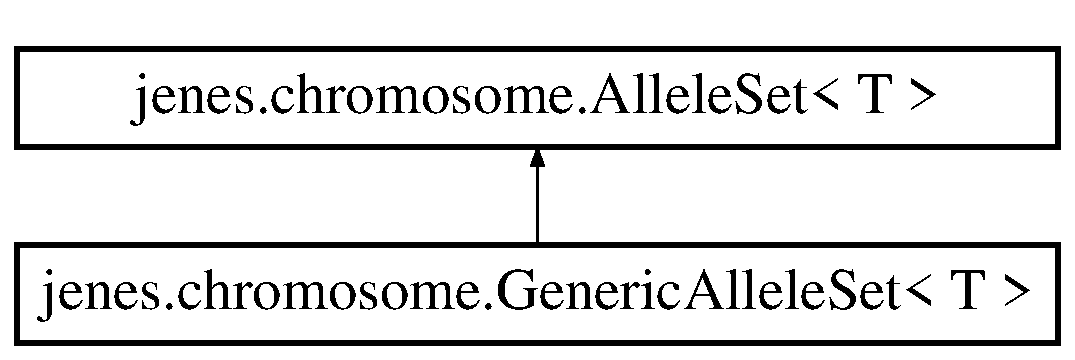
\includegraphics[height=2cm]{classjenes_1_1chromosome_1_1_generic_allele_set_3_01_t_01_4}
\end{center}
\end{figure}
\subsection*{Public Member Functions}
\begin{CompactItemize}
\item 
\hyperlink{classjenes_1_1chromosome_1_1_generic_allele_set_3_01_t_01_4_fc6f6f35af245d54ba7ad6f57a9a3893}{GenericAlleleSet} (final Set$<$ T $>$ set)
\item 
\hyperlink{classjenes_1_1chromosome_1_1_generic_allele_set_3_01_t_01_4_e7a1970427bae039c3f4ae6340b53ca7}{GenericAlleleSet} (final T...values)
\item 
\hyperlink{classjenes_1_1chromosome_1_1_generic_allele_set_3_01_t_01_4_8cbf2394287ce6321fcd338dc4c44a8e}{GenericAlleleSet} (final List$<$ T $>$ list)
\item 
final T \hyperlink{classjenes_1_1chromosome_1_1_generic_allele_set_3_01_t_01_4_cf8f796e2243cc0b745b8d21e45ac7df}{getElementAt} (final int pos)
\item 
final int \hyperlink{classjenes_1_1chromosome_1_1_generic_allele_set_3_01_t_01_4_9b5dd0079f5d0cb76d2f89e92bde3fa6}{getIndexOf} (final T a)
\item 
final T \hyperlink{classjenes_1_1chromosome_1_1_generic_allele_set_3_01_t_01_4_2f330d71d992e0d724bc31730b56229e}{getRandomValue} ()
\item 
final int \hyperlink{classjenes_1_1chromosome_1_1_generic_allele_set_3_01_t_01_4_568ca617716496507d41e348c5bc2845}{size} ()
\item 
void \hyperlink{classjenes_1_1chromosome_1_1_generic_allele_set_3_01_t_01_4_234b0a286a14fcaf0bf10894813465c5}{setDifferences} (double\mbox{[}$\,$\mbox{]}\mbox{[}$\,$\mbox{]} diff)
\item 
double\mbox{[}$\,$\mbox{]}\mbox{[}$\,$\mbox{]} \hyperlink{classjenes_1_1chromosome_1_1_generic_allele_set_3_01_t_01_4_9c24972536c41a2d4660d9cad2694eba}{getDefaultDifferences} ()
\item 
double \hyperlink{classjenes_1_1chromosome_1_1_generic_allele_set_3_01_t_01_4_ce70b10ee535ccc3a7cbcd42739b8d5c}{difference} (T a0, T a1)
\end{CompactItemize}


\subsection{Detailed Description}
A GenericAlleleSet represents a concrete allele set implementation. It is usefull to instantiate a new AlleleSet when the allele values are contained by a list, by an array or by a \hyperlink{}{Set}. At creation time, the aplhabet objects are not cloned so: 

Note that this implementation is not synchronized. If multiple threads access a GenericAlleleSet concurrently, and at least one of the threads modifies the set, it must be synchronized externally or wrapped using the \hyperlink{}{Collections\#synchronizedSet(Set)} method. 

Note that if values are modified externally, the allele set object also change according at that modification. 

Some examples of code are provided below. 

$<$blockquote$>$\small\begin{alltt}
    Set s = Collections.synchronizedSet(new HashSet(...));
    GenericAlleleSet geneticAlleleSet = new GenericAlleleSet(s);
 \end{alltt}
\normalsize 
$<$/blockquote$>$ to build a generic allele set with the object value accesses synchronized. 

$<$blockquote$>$\small\begin{alltt}
    GenericAlleleSet generic alleleSet = new GenericAlleleSet<Boolean>(true, false),
 \end{alltt}
\normalsize 
$<$/blockquote$>$ to build a generic allele set with the boolean values as allele object values. 

$<$blockquote$>$\small\begin{alltt}
    GenericAlleleSet generic alleleSet = new GenericAlleleSet(AnyJavaEnum.values()) );
 \end{alltt}
\normalsize 
$<$/blockquote$>$ to build a generic allele set with the enum values. 

\begin{Desc}
\item[Parameters:]
\begin{description}
\item[{\em $<$T$>$}]\end{description}
\end{Desc}
\begin{Desc}
\item[Version:]2.0 \end{Desc}
\begin{Desc}
\item[Since:]1.0\end{Desc}
\begin{Desc}
\item[See also:]\hyperlink{classjenes_1_1chromosome_1_1_object_chromosome}{jenes.chromosome.ObjectChromosome} \end{Desc}


\subsection{Constructor \& Destructor Documentation}
\hypertarget{classjenes_1_1chromosome_1_1_generic_allele_set_3_01_t_01_4_fc6f6f35af245d54ba7ad6f57a9a3893}{
\index{jenes::chromosome::GenericAlleleSet$<$ T $>$@{jenes::chromosome::GenericAlleleSet$<$ T $>$}!GenericAlleleSet@{GenericAlleleSet}}
\index{GenericAlleleSet@{GenericAlleleSet}!jenes::chromosome::GenericAlleleSet< T >@{jenes::chromosome::GenericAlleleSet$<$ T $>$}}
\subsubsection[GenericAlleleSet]{\setlength{\rightskip}{0pt plus 5cm}jenes.chromosome.GenericAlleleSet$<$ T $>$.GenericAlleleSet (final Set$<$ T $>$ {\em set})}}
\label{classjenes_1_1chromosome_1_1_generic_allele_set_3_01_t_01_4_fc6f6f35af245d54ba7ad6f57a9a3893}


Creates a new AlleleSet instance with the alphabet values contained by the specified set 

\begin{Desc}
\item[Parameters:]
\begin{description}
\item[{\em set}]the set with the alphabet allele values \end{description}
\end{Desc}
\hypertarget{classjenes_1_1chromosome_1_1_generic_allele_set_3_01_t_01_4_e7a1970427bae039c3f4ae6340b53ca7}{
\index{jenes::chromosome::GenericAlleleSet$<$ T $>$@{jenes::chromosome::GenericAlleleSet$<$ T $>$}!GenericAlleleSet@{GenericAlleleSet}}
\index{GenericAlleleSet@{GenericAlleleSet}!jenes::chromosome::GenericAlleleSet< T >@{jenes::chromosome::GenericAlleleSet$<$ T $>$}}
\subsubsection[GenericAlleleSet]{\setlength{\rightskip}{0pt plus 5cm}jenes.chromosome.GenericAlleleSet$<$ T $>$.GenericAlleleSet (final T... {\em values})}}
\label{classjenes_1_1chromosome_1_1_generic_allele_set_3_01_t_01_4_e7a1970427bae039c3f4ae6340b53ca7}


Creates a new AlleleSet instance with the alphabet values contained by the specified array 

\begin{Desc}
\item[Parameters:]
\begin{description}
\item[{\em values}]the alphabet values array \end{description}
\end{Desc}
\hypertarget{classjenes_1_1chromosome_1_1_generic_allele_set_3_01_t_01_4_8cbf2394287ce6321fcd338dc4c44a8e}{
\index{jenes::chromosome::GenericAlleleSet$<$ T $>$@{jenes::chromosome::GenericAlleleSet$<$ T $>$}!GenericAlleleSet@{GenericAlleleSet}}
\index{GenericAlleleSet@{GenericAlleleSet}!jenes::chromosome::GenericAlleleSet< T >@{jenes::chromosome::GenericAlleleSet$<$ T $>$}}
\subsubsection[GenericAlleleSet]{\setlength{\rightskip}{0pt plus 5cm}jenes.chromosome.GenericAlleleSet$<$ T $>$.GenericAlleleSet (final List$<$ T $>$ {\em list})}}
\label{classjenes_1_1chromosome_1_1_generic_allele_set_3_01_t_01_4_8cbf2394287ce6321fcd338dc4c44a8e}


Creates a new AlleleSet instance with the alphabet values contained by the specified list 

\begin{Desc}
\item[Parameters:]
\begin{description}
\item[{\em list}]the alphabet values list \end{description}
\end{Desc}


\subsection{Member Function Documentation}
\hypertarget{classjenes_1_1chromosome_1_1_generic_allele_set_3_01_t_01_4_cf8f796e2243cc0b745b8d21e45ac7df}{
\index{jenes::chromosome::GenericAlleleSet$<$ T $>$@{jenes::chromosome::GenericAlleleSet$<$ T $>$}!getElementAt@{getElementAt}}
\index{getElementAt@{getElementAt}!jenes::chromosome::GenericAlleleSet< T >@{jenes::chromosome::GenericAlleleSet$<$ T $>$}}
\subsubsection[getElementAt]{\setlength{\rightskip}{0pt plus 5cm}final T jenes.chromosome.GenericAlleleSet$<$ T $>$.getElementAt (final int {\em pos})}}
\label{classjenes_1_1chromosome_1_1_generic_allele_set_3_01_t_01_4_cf8f796e2243cc0b745b8d21e45ac7df}


Returns the allele at a given positition. \begin{Desc}
\item[Parameters:]
\begin{description}
\item[{\em pos}]\end{description}
\end{Desc}
\begin{Desc}
\item[Returns:]the element \end{Desc}
\hypertarget{classjenes_1_1chromosome_1_1_generic_allele_set_3_01_t_01_4_9b5dd0079f5d0cb76d2f89e92bde3fa6}{
\index{jenes::chromosome::GenericAlleleSet$<$ T $>$@{jenes::chromosome::GenericAlleleSet$<$ T $>$}!getIndexOf@{getIndexOf}}
\index{getIndexOf@{getIndexOf}!jenes::chromosome::GenericAlleleSet< T >@{jenes::chromosome::GenericAlleleSet$<$ T $>$}}
\subsubsection[getIndexOf]{\setlength{\rightskip}{0pt plus 5cm}final int jenes.chromosome.GenericAlleleSet$<$ T $>$.getIndexOf (final T {\em a})}}
\label{classjenes_1_1chromosome_1_1_generic_allele_set_3_01_t_01_4_9b5dd0079f5d0cb76d2f89e92bde3fa6}


Returns the index of element a.

\begin{Desc}
\item[Parameters:]
\begin{description}
\item[{\em a}]- the allele to find \end{description}
\end{Desc}
\begin{Desc}
\item[Returns:]the allele index \end{Desc}
\hypertarget{classjenes_1_1chromosome_1_1_generic_allele_set_3_01_t_01_4_2f330d71d992e0d724bc31730b56229e}{
\index{jenes::chromosome::GenericAlleleSet$<$ T $>$@{jenes::chromosome::GenericAlleleSet$<$ T $>$}!getRandomValue@{getRandomValue}}
\index{getRandomValue@{getRandomValue}!jenes::chromosome::GenericAlleleSet< T >@{jenes::chromosome::GenericAlleleSet$<$ T $>$}}
\subsubsection[getRandomValue]{\setlength{\rightskip}{0pt plus 5cm}final T jenes.chromosome.GenericAlleleSet$<$ T $>$.getRandomValue ()\hspace{0.3cm}{\tt  \mbox{[}virtual\mbox{]}}}}
\label{classjenes_1_1chromosome_1_1_generic_allele_set_3_01_t_01_4_2f330d71d992e0d724bc31730b56229e}


Returns an allele randomly chosen.

\begin{Desc}
\item[Returns:]a value \end{Desc}


Implements \hyperlink{interfacejenes_1_1chromosome_1_1_allele_set_3_01_t_01_4_c09d409c55d941892df658d21b3d4bff}{jenes.chromosome.AlleleSet$<$ T $>$}.\hypertarget{classjenes_1_1chromosome_1_1_generic_allele_set_3_01_t_01_4_568ca617716496507d41e348c5bc2845}{
\index{jenes::chromosome::GenericAlleleSet$<$ T $>$@{jenes::chromosome::GenericAlleleSet$<$ T $>$}!size@{size}}
\index{size@{size}!jenes::chromosome::GenericAlleleSet< T >@{jenes::chromosome::GenericAlleleSet$<$ T $>$}}
\subsubsection[size]{\setlength{\rightskip}{0pt plus 5cm}final int jenes.chromosome.GenericAlleleSet$<$ T $>$.size ()\hspace{0.3cm}{\tt  \mbox{[}virtual\mbox{]}}}}
\label{classjenes_1_1chromosome_1_1_generic_allele_set_3_01_t_01_4_568ca617716496507d41e348c5bc2845}


Returns the number of alleles held by the allele set.

\begin{Desc}
\item[Returns:]the number of alleles \end{Desc}


Implements \hyperlink{interfacejenes_1_1chromosome_1_1_allele_set_3_01_t_01_4_3acbb10df92ebafc589d5d8546949f2f}{jenes.chromosome.AlleleSet$<$ T $>$}.\hypertarget{classjenes_1_1chromosome_1_1_generic_allele_set_3_01_t_01_4_234b0a286a14fcaf0bf10894813465c5}{
\index{jenes::chromosome::GenericAlleleSet$<$ T $>$@{jenes::chromosome::GenericAlleleSet$<$ T $>$}!setDifferences@{setDifferences}}
\index{setDifferences@{setDifferences}!jenes::chromosome::GenericAlleleSet< T >@{jenes::chromosome::GenericAlleleSet$<$ T $>$}}
\subsubsection[setDifferences]{\setlength{\rightskip}{0pt plus 5cm}void jenes.chromosome.GenericAlleleSet$<$ T $>$.setDifferences (double {\em diff}\mbox{[}$\,$\mbox{]}\mbox{[}$\,$\mbox{]})}}
\label{classjenes_1_1chromosome_1_1_generic_allele_set_3_01_t_01_4_234b0a286a14fcaf0bf10894813465c5}


Sets the difference matrix between alleles. It is expected that diff is a square matrix according to set size, with diff(i,i) = 0 and diff(i,j) = -diff(j,i).

\begin{Desc}
\item[Parameters:]
\begin{description}
\item[{\em diff}]- the difference matrix \end{description}
\end{Desc}
\hypertarget{classjenes_1_1chromosome_1_1_generic_allele_set_3_01_t_01_4_9c24972536c41a2d4660d9cad2694eba}{
\index{jenes::chromosome::GenericAlleleSet$<$ T $>$@{jenes::chromosome::GenericAlleleSet$<$ T $>$}!getDefaultDifferences@{getDefaultDifferences}}
\index{getDefaultDifferences@{getDefaultDifferences}!jenes::chromosome::GenericAlleleSet< T >@{jenes::chromosome::GenericAlleleSet$<$ T $>$}}
\subsubsection[getDefaultDifferences]{\setlength{\rightskip}{0pt plus 5cm}double \mbox{[}$\,$\mbox{]}\mbox{[}$\,$\mbox{]} jenes.chromosome.GenericAlleleSet$<$ T $>$.getDefaultDifferences ()}}
\label{classjenes_1_1chromosome_1_1_generic_allele_set_3_01_t_01_4_9c24972536c41a2d4660d9cad2694eba}


Returns the default difference matrix as given by the difference of allele positions in the set. \begin{Desc}
\item[Returns:]the allele difference matrix. \end{Desc}
\hypertarget{classjenes_1_1chromosome_1_1_generic_allele_set_3_01_t_01_4_ce70b10ee535ccc3a7cbcd42739b8d5c}{
\index{jenes::chromosome::GenericAlleleSet$<$ T $>$@{jenes::chromosome::GenericAlleleSet$<$ T $>$}!difference@{difference}}
\index{difference@{difference}!jenes::chromosome::GenericAlleleSet< T >@{jenes::chromosome::GenericAlleleSet$<$ T $>$}}
\subsubsection[difference]{\setlength{\rightskip}{0pt plus 5cm}double jenes.chromosome.GenericAlleleSet$<$ T $>$.difference (T {\em a0}, \/  T {\em a1})\hspace{0.3cm}{\tt  \mbox{[}virtual\mbox{]}}}}
\label{classjenes_1_1chromosome_1_1_generic_allele_set_3_01_t_01_4_ce70b10ee535ccc3a7cbcd42739b8d5c}


Provides the genetic difference between two alleles.

\begin{Desc}
\item[Parameters:]
\begin{description}
\item[{\em a0}]- first allele \item[{\em a1}]- second allele \end{description}
\end{Desc}
\begin{Desc}
\item[Returns:]- the genetic difeerence \end{Desc}


Implements \hyperlink{interfacejenes_1_1chromosome_1_1_allele_set_3_01_t_01_4_74ab0cb120fcfdee8e878727d6c50815}{jenes.chromosome.AlleleSet$<$ T $>$}.

The documentation for this class was generated from the following file:\begin{CompactItemize}
\item 
src/jenes/chromosome/GenericAlleleSet.java\end{CompactItemize}

\hypertarget{classjenes_1_1_genetic_algorithm_3_01_t_01extends_01_chromosome_01_4}{
\section{jenes.GeneticAlgorithm$<$ T extends Chromosome $>$ Class Reference}
\label{classjenes_1_1_genetic_algorithm_3_01_t_01extends_01_chromosome_01_4}\index{jenes::GeneticAlgorithm$<$ T extends Chromosome $>$@{jenes::GeneticAlgorithm$<$ T extends Chromosome $>$}}
}
\subsection*{Public Types}
\begin{CompactItemize}
\item 
enum \hyperlink{classjenes_1_1_genetic_algorithm_3_01_t_01extends_01_chromosome_01_4_afb755e144130d2c2c6ca86134dd871e}{ElitismStrategy} \{ \hyperlink{_genetic_algorithm_8java_afb755e144130d2c2c6ca86134dd871ea2b65445a3a16f164c5e811064d75726}{RANDOM}, 
\hyperlink{_genetic_algorithm_8java_afb755e144130d2c2c6ca86134dd871eed58eb79392224559f176f4794c570e1}{WORST}
 \}
\item 
enum \hyperlink{classjenes_1_1_genetic_algorithm_3_01_t_01extends_01_chromosome_01_4_49749d00b9417b958d1b30e08fc21d53}{ResizeStrategy} \{ \hyperlink{_genetic_algorithm_8java_49749d00b9417b958d1b30e08fc21d53c157bdf0b85a40d2619cbc8bc1ae5fe2}{NONE}, 
\hyperlink{_genetic_algorithm_8java_49749d00b9417b958d1b30e08fc21d53eef9468d1b98bca652a04bf5063fd9d6}{AUTO}, 
\hyperlink{_genetic_algorithm_8java_49749d00b9417b958d1b30e08fc21d532f0d18fc0d0fa4a6cd92dc328501874d}{EMPTY}
 \}
\end{CompactItemize}
\subsection*{Public Member Functions}
\begin{CompactItemize}
\item 
\hyperlink{classjenes_1_1_genetic_algorithm_3_01_t_01extends_01_chromosome_01_4_cfda239e0d2154eb26a7be4f6aa1315d}{GeneticAlgorithm} ()
\item 
\hyperlink{classjenes_1_1_genetic_algorithm_3_01_t_01extends_01_chromosome_01_4_ede3d2fbd3c3d1cf04a4e419649cae93}{GeneticAlgorithm} (final Population$<$ T $>$ pop)
\item 
\hyperlink{classjenes_1_1_genetic_algorithm_3_01_t_01extends_01_chromosome_01_4_fe0501230c1645d2a6cdf54af2672639}{GeneticAlgorithm} (final Population$<$ T $>$ pop, final int genlimit)
\item 
\hyperlink{classjenes_1_1_genetic_algorithm_3_01_t_01extends_01_chromosome_01_4_efcf45276a730906c98ff8de90b6c48e}{GeneticAlgorithm} (final Fitness fitness)
\item 
\hyperlink{classjenes_1_1_genetic_algorithm_3_01_t_01extends_01_chromosome_01_4_08a57814b09412baed3146d2cc6e2174}{GeneticAlgorithm} (final Fitness fitness, final Population$<$ T $>$ pop)
\item 
\hyperlink{classjenes_1_1_genetic_algorithm_3_01_t_01extends_01_chromosome_01_4_f3997e737162629c161c04a65dd830a0}{GeneticAlgorithm} (final Fitness fitness, final Population$<$ T $>$ pop, final int genlimit)
\item 
final Fitness \hyperlink{classjenes_1_1_genetic_algorithm_3_01_t_01extends_01_chromosome_01_4_687996ee45582145be24e2086fc8c210}{getFitness} ()
\item 
final void \hyperlink{classjenes_1_1_genetic_algorithm_3_01_t_01extends_01_chromosome_01_4_ff762153c3f11a2ad83936867ca31617}{setFitness} (Fitness fitness)
\item 
final boolean \hyperlink{classjenes_1_1_genetic_algorithm_3_01_t_01extends_01_chromosome_01_4_7d5cb4716cbc586aa85774c5dc934d15}{isFitnessChanged} ()
\item 
\hyperlink{classjenes_1_1utils_1_1multitasking_1_1_runner}{Runner} \hyperlink{classjenes_1_1_genetic_algorithm_3_01_t_01extends_01_chromosome_01_4_63ea13380fe4a30d1eabd394e44d6e96}{getRunner} ()
\item 
void \hyperlink{classjenes_1_1_genetic_algorithm_3_01_t_01extends_01_chromosome_01_4_6ff8bcd8e9049106c7959637e4e10e70}{setRunner} (\hyperlink{classjenes_1_1utils_1_1multitasking_1_1_runner}{Runner} runner)
\item 
void \hyperlink{classjenes_1_1_genetic_algorithm_3_01_t_01extends_01_chromosome_01_4_7e5f06abe9e8661cdb38bd0fa663da6c}{setRandomSeed} (long seed)
\item 
final int \hyperlink{classjenes_1_1_genetic_algorithm_3_01_t_01extends_01_chromosome_01_4_b52be3b0fcd2f424ae191ff4e642edf3}{getHistorySize} ()
\item 
final Pool$<$ T $>$ \hyperlink{classjenes_1_1_genetic_algorithm_3_01_t_01extends_01_chromosome_01_4_d254fc6b2ff476bc7f7837d03e677786}{getPool} ()
\item 
void \hyperlink{classjenes_1_1_genetic_algorithm_3_01_t_01extends_01_chromosome_01_4_71407144e93e7522d2d474c25781d65c}{setHistorySize} (int hs)
\item 
final Population$<$ T $>$ \hyperlink{classjenes_1_1_genetic_algorithm_3_01_t_01extends_01_chromosome_01_4_99718490498059da48833dfbdfc8076e}{getHistoryAt} (int pos)
\item 
final Population$<$ T $>$ \hyperlink{classjenes_1_1_genetic_algorithm_3_01_t_01extends_01_chromosome_01_4_b5ff704fa1d7b01bcfc5f0ca36b20e34}{getInitialPopulation} ()
\item 
final Population$<$ T $>$ \hyperlink{classjenes_1_1_genetic_algorithm_3_01_t_01extends_01_chromosome_01_4_855bc56ffb3e1704ced2fdf68cc96d8f}{getCurrentPopulation} ()
\item 
final Population$<$ T $>$ \hyperlink{classjenes_1_1_genetic_algorithm_3_01_t_01extends_01_chromosome_01_4_5d22b21350638a64a66d3599b2777982}{getNextPopulation} ()
\item 
final void \hyperlink{classjenes_1_1_genetic_algorithm_3_01_t_01extends_01_chromosome_01_4_8afdd855dc891b981cbf675c63db72c3}{evolve} ()  throws AlgorithmException 
\item 
final void \hyperlink{classjenes_1_1_genetic_algorithm_3_01_t_01extends_01_chromosome_01_4_fea32755ac446883e283d2eec6bc69fa}{evolve} (final Population$<$ T $>$ pop)
\item 
final void \hyperlink{classjenes_1_1_genetic_algorithm_3_01_t_01extends_01_chromosome_01_4_f8bb6842d525c274bfb8a3efc9ca5b23}{evolve} (boolean restart)  throws AlgorithmException 
\item 
final void \hyperlink{classjenes_1_1_genetic_algorithm_3_01_t_01extends_01_chromosome_01_4_b90dc099bae1616275779f59f400a59b}{evaluatePopulation} (final Population$<$ T $>$ population)
\item 
final void \hyperlink{classjenes_1_1_genetic_algorithm_3_01_t_01extends_01_chromosome_01_4_4a04df077e2b7752248689668889a5a5}{evaluatePopulation} (final Population$<$ T $>$ population, final boolean forced)
\item 
void \hyperlink{classjenes_1_1_genetic_algorithm_3_01_t_01extends_01_chromosome_01_4_17d1c99e638312a18394c6d76dedb2f3}{evaluateIndividual} (final Individual$<$ T $>$ individual)
\item 
final void \hyperlink{classjenes_1_1_genetic_algorithm_3_01_t_01extends_01_chromosome_01_4_cf14a43bc2c8bed69aa0334b18d58ba7}{setRandomization} (final boolean value)
\item 
void \hyperlink{classjenes_1_1_genetic_algorithm_3_01_t_01extends_01_chromosome_01_4_78cb20ba6256d06e7cd04696e697cc4e}{setRandomization} (final double rate)
\item 
final double \hyperlink{classjenes_1_1_genetic_algorithm_3_01_t_01extends_01_chromosome_01_4_dd75e6182615af89791921472d2fbc9f}{getRandomization} ()
\item 
final int \hyperlink{classjenes_1_1_genetic_algorithm_3_01_t_01extends_01_chromosome_01_4_25602ec654959a43a64f12e92251cb47}{getGeneration} ()
\item 
final int \hyperlink{classjenes_1_1_genetic_algorithm_3_01_t_01extends_01_chromosome_01_4_c6eceff2ad4a055f3c6047fb4c272ef3}{getGenerationLimit} ()
\item 
void \hyperlink{classjenes_1_1_genetic_algorithm_3_01_t_01extends_01_chromosome_01_4_1e4d04de7cf34838296ad6745ac046f5}{setGenerationLimit} (final int limit)
\item 
void \hyperlink{classjenes_1_1_genetic_algorithm_3_01_t_01extends_01_chromosome_01_4_a0ab85fdb0cb1880a469044affbb32e7}{addStage} (final AbstractStage$<$ T $>$ stage)
\item 
final boolean \hyperlink{classjenes_1_1_genetic_algorithm_3_01_t_01extends_01_chromosome_01_4_34e6ea627850ec240d4c0bba39170d4b}{isBiggerBetter} ()
\item 
void \hyperlink{classjenes_1_1_genetic_algorithm_3_01_t_01extends_01_chromosome_01_4_fcc4f944d2d47d757e177a22a660bfd3}{setBiggerIsBetter} (final boolean flag)
\item 
boolean \hyperlink{classjenes_1_1_genetic_algorithm_3_01_t_01extends_01_chromosome_01_4_7305deb720716287d256832f0bd44785}{isFullEvaluationForced} ()
\item 
void \hyperlink{classjenes_1_1_genetic_algorithm_3_01_t_01extends_01_chromosome_01_4_9fe6f2d66ffcbce1233194871cdfc5ae}{setFullEvaluationForced} (boolean flag)
\item 
final int \hyperlink{classjenes_1_1_genetic_algorithm_3_01_t_01extends_01_chromosome_01_4_8bbf6df4fc231cfc88a7e879d2bbf814}{getElitism} ()
\item 
void \hyperlink{classjenes_1_1_genetic_algorithm_3_01_t_01extends_01_chromosome_01_4_27f67506714b18eb15d890bfa3d5b0ab}{setElitism} (final int \hyperlink{classjenes_1_1_genetic_algorithm_3_01_t_01extends_01_chromosome_01_4_c4280b01e7da0ddc049050b19e28b8b9}{elitism})
\item 
final \hyperlink{classjenes_1_1_genetic_algorithm_3_01_t_01extends_01_chromosome_01_4_afb755e144130d2c2c6ca86134dd871e}{ElitismStrategy} \hyperlink{classjenes_1_1_genetic_algorithm_3_01_t_01extends_01_chromosome_01_4_d227ba9924206ee18f69d24ea4ee4ab0}{getElitismStrategy} ()
\item 
void \hyperlink{classjenes_1_1_genetic_algorithm_3_01_t_01extends_01_chromosome_01_4_edc89ba915f6a528ef4052eb31a8c467}{setElitismStrategy} (final \hyperlink{classjenes_1_1_genetic_algorithm_3_01_t_01extends_01_chromosome_01_4_afb755e144130d2c2c6ca86134dd871e}{ElitismStrategy} es)
\item 
void \hyperlink{classjenes_1_1_genetic_algorithm_3_01_t_01extends_01_chromosome_01_4_685af9b6322920d9431977fd25c5cf77}{setResizeStrategy} (final \hyperlink{classjenes_1_1_genetic_algorithm_3_01_t_01extends_01_chromosome_01_4_49749d00b9417b958d1b30e08fc21d53}{ResizeStrategy} rs)
\item 
final \hyperlink{classjenes_1_1_genetic_algorithm_3_01_t_01extends_01_chromosome_01_4_49749d00b9417b958d1b30e08fc21d53}{ResizeStrategy} \hyperlink{classjenes_1_1_genetic_algorithm_3_01_t_01extends_01_chromosome_01_4_379c5a3789ba72941a081d32fbcc4474}{getResizeStrategy} ()
\item 
final Sequence$<$ T $>$ \hyperlink{classjenes_1_1_genetic_algorithm_3_01_t_01extends_01_chromosome_01_4_eab54a329fb6df5686a2fce4a8a8727a}{getBody} ()
\item 
final void \hyperlink{classjenes_1_1_genetic_algorithm_3_01_t_01extends_01_chromosome_01_4_168e2b37b5351108e62d8fb887e1fae4}{addAlgorithmEventListener} (final AlgorithmEventListener$<$ T $>$ ael)
\item 
final void \hyperlink{classjenes_1_1_genetic_algorithm_3_01_t_01extends_01_chromosome_01_4_8cab61e04f54ed5abbda047815a1683d}{removeAlgorithmEventListener} (final AlgorithmEventListener ael)
\item 
final void \hyperlink{classjenes_1_1_genetic_algorithm_3_01_t_01extends_01_chromosome_01_4_a39f1ae905e67a5a3f7d7ad5cb25d276}{addGenerationEventListener} (final GenerationEventListener$<$ T $>$ gel)
\item 
final void \hyperlink{classjenes_1_1_genetic_algorithm_3_01_t_01extends_01_chromosome_01_4_33e632148218289d0bc43e202a804bf1}{removeGenerationEventListener} (final GenerationEventListener gel)
\item 
final Statistics \hyperlink{classjenes_1_1_genetic_algorithm_3_01_t_01extends_01_chromosome_01_4_484fcdba7cf2e4aa4a6ec1c0006e2193}{getStatistics} ()
\item 
final void \hyperlink{classjenes_1_1_genetic_algorithm_3_01_t_01extends_01_chromosome_01_4_8a4f4965c968047c55a8b56240267a4f}{updateStatistics} (final Statistics stats)
\item 
\hypertarget{classjenes_1_1_genetic_algorithm_3_01_t_01extends_01_chromosome_01_4_f847a2a8cba2288fbddf726ec12eaf47}{
final String \textbf{toString} ()}
\label{classjenes_1_1_genetic_algorithm_3_01_t_01extends_01_chromosome_01_4_f847a2a8cba2288fbddf726ec12eaf47}

\end{CompactItemize}
\subsection*{Static Public Attributes}
\begin{CompactItemize}
\item 
static final int \hyperlink{classjenes_1_1_genetic_algorithm_3_01_t_01extends_01_chromosome_01_4_2492ee1b00f5631a1c1b1c6f15ea3421}{DEFAULT\_\-GENERATION\_\-LIMIT} = 100
\item 
static final int \hyperlink{classjenes_1_1_genetic_algorithm_3_01_t_01extends_01_chromosome_01_4_23df2e338c3439d7457ff6a150c573e1}{DEFAULT\_\-HISTORY\_\-SIZE} = 2
\item 
static final int \hyperlink{classjenes_1_1_genetic_algorithm_3_01_t_01extends_01_chromosome_01_4_a64b297086826bfbda1fbaccebe4cb24}{MIN\_\-HISTORY\_\-SIZE} = 2
\item 
static final int \hyperlink{classjenes_1_1_genetic_algorithm_3_01_t_01extends_01_chromosome_01_4_cd26085cf69c68d607ef08d0bf829224}{MAX\_\-HISTORY\_\-SIZE} = 100
\end{CompactItemize}
\subsection*{Protected Member Functions}
\begin{CompactItemize}
\item 
boolean \hyperlink{classjenes_1_1_genetic_algorithm_3_01_t_01extends_01_chromosome_01_4_41376d72c82d4503693eebb3832cf772}{end} ()
\item 
final void \hyperlink{classjenes_1_1_genetic_algorithm_3_01_t_01extends_01_chromosome_01_4_6fd4badfc67b0c2b0d43c6dd4a14875e}{start} (boolean reset)
\item 
final void \hyperlink{classjenes_1_1_genetic_algorithm_3_01_t_01extends_01_chromosome_01_4_6d0de9962bff7d63a4c197eeef6da7d0}{stop} ()
\item 
void \hyperlink{classjenes_1_1_genetic_algorithm_3_01_t_01extends_01_chromosome_01_4_0ed4a97cf7e3266913eaad8092913de3}{onStart} (long time)
\item 
void \hyperlink{classjenes_1_1_genetic_algorithm_3_01_t_01extends_01_chromosome_01_4_85479397ce0f8bd995b97fa91f4d6690}{onInit} (long time)
\item 
void \hyperlink{classjenes_1_1_genetic_algorithm_3_01_t_01extends_01_chromosome_01_4_04258af6f64ec98561b015651d20f9ea}{onStop} (long time)
\item 
void \hyperlink{classjenes_1_1_genetic_algorithm_3_01_t_01extends_01_chromosome_01_4_ed0d630f1e0b290bb87ba9ab8b164b89}{onGeneration} (long time)
\item 
final void \hyperlink{classjenes_1_1_genetic_algorithm_3_01_t_01extends_01_chromosome_01_4_7824bcf504331528000af8be62073d53}{randomizePopulation} (final Population$<$ T $>$ pop)
\item 
void \hyperlink{classjenes_1_1_genetic_algorithm_3_01_t_01extends_01_chromosome_01_4_7cefcc35bf6c98eb9b7c33c074b32d69}{randomizeIndividual} (final Individual$<$ T $>$ individual)
\item 
final void \hyperlink{classjenes_1_1_genetic_algorithm_3_01_t_01extends_01_chromosome_01_4_85647664d61cca550ed40dd70b074365}{applyElitism} ()
\end{CompactItemize}
\subsection*{Protected Attributes}
\begin{CompactItemize}
\item 
Sequence$<$ T $>$ \hyperlink{classjenes_1_1_genetic_algorithm_3_01_t_01extends_01_chromosome_01_4_0040f9dbb0018e8bb28dde97dacac7d8}{body}
\item 
Statistics \hyperlink{classjenes_1_1_genetic_algorithm_3_01_t_01extends_01_chromosome_01_4_fc23d5cbab5434f5ec5684cda9434b93}{statistics} = null
\item 
int \hyperlink{classjenes_1_1_genetic_algorithm_3_01_t_01extends_01_chromosome_01_4_c5a1ddc5e78e2b81c754eb990a91f17b}{generation} = 0
\item 
double \hyperlink{classjenes_1_1_genetic_algorithm_3_01_t_01extends_01_chromosome_01_4_dcb3e16398451c2e318de21d77b51d35}{randomization} = 1.0
\item 
int \hyperlink{classjenes_1_1_genetic_algorithm_3_01_t_01extends_01_chromosome_01_4_6677c80cf6ad470a0124fc2fa3051310}{generationLimit}
\item 
int \hyperlink{classjenes_1_1_genetic_algorithm_3_01_t_01extends_01_chromosome_01_4_c4280b01e7da0ddc049050b19e28b8b9}{elitism} = 0
\item 
\hyperlink{classjenes_1_1_genetic_algorithm_3_01_t_01extends_01_chromosome_01_4_afb755e144130d2c2c6ca86134dd871e}{ElitismStrategy} \hyperlink{classjenes_1_1_genetic_algorithm_3_01_t_01extends_01_chromosome_01_4_acba3e1823ba66a2dd6d3c902f8ff719}{elitismStrategy} = ElitismStrategy.WORST
\item 
Population$<$ T $>$ \hyperlink{classjenes_1_1_genetic_algorithm_3_01_t_01extends_01_chromosome_01_4_b6535da7a5097e18e6305d0f26f7cf5f}{initialPopulation} = null
\item 
List$<$ AlgorithmEventListener$<$ T $>$ $>$ \hyperlink{classjenes_1_1_genetic_algorithm_3_01_t_01extends_01_chromosome_01_4_53540867ddd13889614232b3cbea6d6f}{algorithmListeners}
\item 
List$<$ GenerationEventListener$<$ T $>$ $>$ \hyperlink{classjenes_1_1_genetic_algorithm_3_01_t_01extends_01_chromosome_01_4_265c4e10d321e68ae5757abf68d88739}{generationListeners}
\item 
\hyperlink{classjenes_1_1_genetic_algorithm_3_01_t_01extends_01_chromosome_01_4_49749d00b9417b958d1b30e08fc21d53}{ResizeStrategy} \hyperlink{classjenes_1_1_genetic_algorithm_3_01_t_01extends_01_chromosome_01_4_56f08a1d1f3355921b83f08745dbb3b3}{resizeStrategy} = ResizeStrategy.AUTO
\item 
boolean \hyperlink{classjenes_1_1_genetic_algorithm_3_01_t_01extends_01_chromosome_01_4_db627d0c6d6744f53ef5c3b7506913e9}{fullEvaluationForced} = false
\item 
\hyperlink{classjenes_1_1utils_1_1_random}{Random} \hyperlink{classjenes_1_1_genetic_algorithm_3_01_t_01extends_01_chromosome_01_4_1579283e210144ba90b937be0911a028}{random} = Random.getInstance()
\end{CompactItemize}
\subsection*{Classes}
\begin{CompactItemize}
\item 
class \textbf{Statistics}
\end{CompactItemize}


\subsection{Detailed Description}
This is the main class of JENES, providing the skeleton for implementing genetic algorithms. 

A genetic algorithm can be implemented by providing a {\tt Fitness} function. An alternative way (but deprecated) is to subclass {\tt GeneticAlgorithm} and to overwrite the method \hyperlink{}{evaluateIndividual(Individual)}. 

The genetic algorithm body is made of a sequence of stages. Which stages and in which order to consider is left to the algorithm needs. Generally, the sequence is made of a selection operator, followed by a a crossover operator, and then by a mutation operator. This schema is implemented by \hyperlink{}{jenes.algorithms.SimpleGA}. 

An example of code is provided below. First, the initial population has to be created. 

$<$blockquote$>$

\small\begin{alltt}
 BooleanChromosome chrom = new BooleanChromosome(CHROMOSOME\_LENGTH);
 Individual<BooleanChromosome> ind = new Individual<BooleanChromosome>(chrom);
 Population<BooleanChromosome> pop = new Population<BooleanChromosome>(ind,
 		POPULATION\_SIZE);
 \end{alltt}
\normalsize 


$<$/blockquote$>$ 

A fitness function is implmented.

$<$blockquote$>$ \small\begin{alltt}
 Fitness<BooleanChromosome> fit = new Fitness<BooleanChromosome>(true) \{\end{alltt}
\normalsize 


\small\begin{alltt}     
     public void evaluate(Individual<BooleanChromosome> individual) \{
         BooleanChromosome chrom = individual.getChromosome();
         int count = 0;
         int length=chrom.length();
         for(int i=0;i<length;i++)
             if(chrom.getValue(i))
                 count++;\end{alltt}
\normalsize 


\small\begin{alltt}             individual.setScore(count);
          \}           
     \};
 \end{alltt}
\normalsize 
 $<$/blockquote$>$

Then, the genetic algorithm is instanced. 

$<$blockquote$>$

\small\begin{alltt}
 GeneticAlgorithm<BooleanChromosome> ga = new GeneticAlgorithm<BooleanChromosome>(fit, pop, GENERATION\_LIMIT);
 \end{alltt}
\normalsize 


$<$/blockquote$>$ 

In this example, we used an anonymous subclass, but other subclassing methods can be used. After, stages (operators in particular) are added to the algorithm's body. 

$<$blockquote$>$

\small\begin{alltt}
 AbstractStage<BooleanChromosome> selection = new TournamentSelector<BooleanChromosome>(3);
 AbstractStage<BooleanChromosome> crossover = new OnePointCrossover<BooleanChromosome>(0.8);
 AbstractStage<BooleanChromosome> mutation = new SimpleMutator<BooleanChromosome>(0.2);\end{alltt}
\normalsize 


\small\begin{alltt} ga.addStage(selection);
 ga.addStage(crossover);
 ga.addStage(mutation);
 \end{alltt}
\normalsize 


$<$/blockquote$>$ 

Finally, the algorithm is executed. 

$<$blockquote$>$

\small\begin{alltt}
 ga.evolve();
 \end{alltt}
\normalsize 


$<$/blockquote$>$ 

A genetic algorithm processes a \hyperlink{}{Population} of \hyperlink{}{Individual}s. At each generation there are an input and output population. The reference to these populations can be respectively obtained by the methods \hyperlink{classjenes_1_1_genetic_algorithm_3_01_t_01extends_01_chromosome_01_4_855bc56ffb3e1704ced2fdf68cc96d8f}{getCurrentPopulation()} and \hyperlink{classjenes_1_1_genetic_algorithm_3_01_t_01extends_01_chromosome_01_4_5d22b21350638a64a66d3599b2777982}{getNextPopulation()}. Past populations are buffered in the algorithm's history. An history population can be retrieve by the method \hyperlink{classjenes_1_1_genetic_algorithm_3_01_t_01extends_01_chromosome_01_4_99718490498059da48833dfbdfc8076e}{getHistoryAt(int)}. The reference to an history population is valid for the history length. After, populations are collected for reuse, so references to them are not anymore valid. 

The genetic algorithm execution is invoked by the method \hyperlink{classjenes_1_1_genetic_algorithm_3_01_t_01extends_01_chromosome_01_4_8afdd855dc891b981cbf675c63db72c3}{evolve()}. The algorithm execution passes through the following events: \begin{itemize}
\item Start: the algorithm is just created. \item Init: internal structures, such as the population given as input at generation 0 and history, are initialized. \item Generation: a generation has been just performed. \item Stop: the algorithm terminates its executions. \end{itemize}
Each of these events can be captured by \hyperlink{}{AlgorithmEventListener}s and \hyperlink{}{GenerationEventListener}s. They can also be caputured by the {\tt GeneticAlgorithm} subclass, by overriding the methods \hyperlink{classjenes_1_1_genetic_algorithm_3_01_t_01extends_01_chromosome_01_4_0ed4a97cf7e3266913eaad8092913de3}{onStart}, \hyperlink{classjenes_1_1_genetic_algorithm_3_01_t_01extends_01_chromosome_01_4_85479397ce0f8bd995b97fa91f4d6690}{onInit}, \hyperlink{classjenes_1_1_genetic_algorithm_3_01_t_01extends_01_chromosome_01_4_ed0d630f1e0b290bb87ba9ab8b164b89}{onGeneration}, and \hyperlink{classjenes_1_1_genetic_algorithm_3_01_t_01extends_01_chromosome_01_4_04258af6f64ec98561b015651d20f9ea}{onStop}. Capturing events is useful to collect statistics and to perform analyses. Evolution terminates when the maximum number of generations is reached. It is possible to terminate the execution on the basis of some condition (e.g. precision level, variance of population, ecc.) by overriding the method \hyperlink{classjenes_1_1_genetic_algorithm_3_01_t_01extends_01_chromosome_01_4_41376d72c82d4503693eebb3832cf772}{end()}. 

{\tt GeneticAlgorithm} include a support for elitism, that is best individuals at each generation are assured to be at the next generation. The number of elite individuals is set by the method \hyperlink{}{setElitism(int)}. These individuals are substituted to some individuals to the processed population according to the following strategies: \begin{itemize}
\item \hyperlink{}{ElitismStrategy\#RANDOM}: next population individuals are randomly selected and substituted by elite. \item \hyperlink{}{ElitismStrategy\#WORST}: next population worst individuals are substituted by elite. \end{itemize}
The first strategy is more efficient as it does not require to order the population. The drawback is that individuals with a good fitness could be substituted by elite. The second strategy is slower, but assures that only worst individuals are substituted. 

The genetic algorithm can be used for both maximizing or minimizing the fitness function. This can be accomplished by setting the fitness. 

{\tt GeneticAlgorithm} can process populations with a variable number of individuals at each generation. 

{\tt GeneticAlgorithm} performs by default an initial randomization of the population. 

\begin{Desc}
\item[Parameters:]
\begin{description}
\item[{\em $<$T$>$}]The class of chromosomes to work with.\end{description}
\end{Desc}
\begin{Desc}
\item[Version:]2.0 \end{Desc}
\begin{Desc}
\item[Since:]1.0 \end{Desc}


\subsection{Member Enumeration Documentation}
\hypertarget{classjenes_1_1_genetic_algorithm_3_01_t_01extends_01_chromosome_01_4_afb755e144130d2c2c6ca86134dd871e}{
\index{jenes::GeneticAlgorithm$<$ T extends Chromosome $>$@{jenes::GeneticAlgorithm$<$ T extends Chromosome $>$}!ElitismStrategy@{ElitismStrategy}}
\index{ElitismStrategy@{ElitismStrategy}!jenes::GeneticAlgorithm< T extends Chromosome >@{jenes::GeneticAlgorithm$<$ T extends Chromosome $>$}}
\subsubsection[ElitismStrategy]{\setlength{\rightskip}{0pt plus 5cm}enum jenes::GeneticAlgorithm$<$ T extends Chromosome $>$::{\bf ElitismStrategy}}}
\label{classjenes_1_1_genetic_algorithm_3_01_t_01extends_01_chromosome_01_4_afb755e144130d2c2c6ca86134dd871e}


The elitism strategy enumeration \hypertarget{classjenes_1_1_genetic_algorithm_3_01_t_01extends_01_chromosome_01_4_49749d00b9417b958d1b30e08fc21d53}{
\index{jenes::GeneticAlgorithm$<$ T extends Chromosome $>$@{jenes::GeneticAlgorithm$<$ T extends Chromosome $>$}!ResizeStrategy@{ResizeStrategy}}
\index{ResizeStrategy@{ResizeStrategy}!jenes::GeneticAlgorithm< T extends Chromosome >@{jenes::GeneticAlgorithm$<$ T extends Chromosome $>$}}
\subsubsection[ResizeStrategy]{\setlength{\rightskip}{0pt plus 5cm}enum jenes::GeneticAlgorithm$<$ T extends Chromosome $>$::{\bf ResizeStrategy}}}
\label{classjenes_1_1_genetic_algorithm_3_01_t_01extends_01_chromosome_01_4_49749d00b9417b958d1b30e08fc21d53}


The resize stategy enumeration. It is used in \hyperlink{}{jenes.stage.Sequence}

\subsection{Constructor \& Destructor Documentation}
\hypertarget{classjenes_1_1_genetic_algorithm_3_01_t_01extends_01_chromosome_01_4_cfda239e0d2154eb26a7be4f6aa1315d}{
\index{jenes::GeneticAlgorithm$<$ T extends Chromosome $>$@{jenes::GeneticAlgorithm$<$ T extends Chromosome $>$}!GeneticAlgorithm@{GeneticAlgorithm}}
\index{GeneticAlgorithm@{GeneticAlgorithm}!jenes::GeneticAlgorithm< T extends Chromosome >@{jenes::GeneticAlgorithm$<$ T extends Chromosome $>$}}
\subsubsection[GeneticAlgorithm]{\setlength{\rightskip}{0pt plus 5cm}jenes.GeneticAlgorithm$<$ T extends Chromosome $>$.GeneticAlgorithm ()}}
\label{classjenes_1_1_genetic_algorithm_3_01_t_01extends_01_chromosome_01_4_cfda239e0d2154eb26a7be4f6aa1315d}


Constructs a new genetic algorithm with no initial population and the default generation limit. \hypertarget{classjenes_1_1_genetic_algorithm_3_01_t_01extends_01_chromosome_01_4_ede3d2fbd3c3d1cf04a4e419649cae93}{
\index{jenes::GeneticAlgorithm$<$ T extends Chromosome $>$@{jenes::GeneticAlgorithm$<$ T extends Chromosome $>$}!GeneticAlgorithm@{GeneticAlgorithm}}
\index{GeneticAlgorithm@{GeneticAlgorithm}!jenes::GeneticAlgorithm< T extends Chromosome >@{jenes::GeneticAlgorithm$<$ T extends Chromosome $>$}}
\subsubsection[GeneticAlgorithm]{\setlength{\rightskip}{0pt plus 5cm}jenes.GeneticAlgorithm$<$ T extends Chromosome $>$.GeneticAlgorithm (final Population$<$ T $>$ {\em pop})}}
\label{classjenes_1_1_genetic_algorithm_3_01_t_01extends_01_chromosome_01_4_ede3d2fbd3c3d1cf04a4e419649cae93}


Constructs a new genetic algorithm with the specified population and the default generation limit. 

\begin{Desc}
\item[Parameters:]
\begin{description}
\item[{\em pop}]the sample population \end{description}
\end{Desc}
\hypertarget{classjenes_1_1_genetic_algorithm_3_01_t_01extends_01_chromosome_01_4_fe0501230c1645d2a6cdf54af2672639}{
\index{jenes::GeneticAlgorithm$<$ T extends Chromosome $>$@{jenes::GeneticAlgorithm$<$ T extends Chromosome $>$}!GeneticAlgorithm@{GeneticAlgorithm}}
\index{GeneticAlgorithm@{GeneticAlgorithm}!jenes::GeneticAlgorithm< T extends Chromosome >@{jenes::GeneticAlgorithm$<$ T extends Chromosome $>$}}
\subsubsection[GeneticAlgorithm]{\setlength{\rightskip}{0pt plus 5cm}jenes.GeneticAlgorithm$<$ T extends Chromosome $>$.GeneticAlgorithm (final Population$<$ T $>$ {\em pop}, \/  final int {\em genlimit})}}
\label{classjenes_1_1_genetic_algorithm_3_01_t_01extends_01_chromosome_01_4_fe0501230c1645d2a6cdf54af2672639}


Constructs a new genetic algorithm with the specified population and the specified generation limit. 

\begin{Desc}
\item[Parameters:]
\begin{description}
\item[{\em pop}]the sample population \item[{\em genlimit}]the generations upper bound \end{description}
\end{Desc}
\hypertarget{classjenes_1_1_genetic_algorithm_3_01_t_01extends_01_chromosome_01_4_efcf45276a730906c98ff8de90b6c48e}{
\index{jenes::GeneticAlgorithm$<$ T extends Chromosome $>$@{jenes::GeneticAlgorithm$<$ T extends Chromosome $>$}!GeneticAlgorithm@{GeneticAlgorithm}}
\index{GeneticAlgorithm@{GeneticAlgorithm}!jenes::GeneticAlgorithm< T extends Chromosome >@{jenes::GeneticAlgorithm$<$ T extends Chromosome $>$}}
\subsubsection[GeneticAlgorithm]{\setlength{\rightskip}{0pt plus 5cm}jenes.GeneticAlgorithm$<$ T extends Chromosome $>$.GeneticAlgorithm (final Fitness {\em fitness})}}
\label{classjenes_1_1_genetic_algorithm_3_01_t_01extends_01_chromosome_01_4_efcf45276a730906c98ff8de90b6c48e}


Constructs a new genetic algorithm with no initial population and the default generation limit. \hypertarget{classjenes_1_1_genetic_algorithm_3_01_t_01extends_01_chromosome_01_4_08a57814b09412baed3146d2cc6e2174}{
\index{jenes::GeneticAlgorithm$<$ T extends Chromosome $>$@{jenes::GeneticAlgorithm$<$ T extends Chromosome $>$}!GeneticAlgorithm@{GeneticAlgorithm}}
\index{GeneticAlgorithm@{GeneticAlgorithm}!jenes::GeneticAlgorithm< T extends Chromosome >@{jenes::GeneticAlgorithm$<$ T extends Chromosome $>$}}
\subsubsection[GeneticAlgorithm]{\setlength{\rightskip}{0pt plus 5cm}jenes.GeneticAlgorithm$<$ T extends Chromosome $>$.GeneticAlgorithm (final Fitness {\em fitness}, \/  final Population$<$ T $>$ {\em pop})}}
\label{classjenes_1_1_genetic_algorithm_3_01_t_01extends_01_chromosome_01_4_08a57814b09412baed3146d2cc6e2174}


Constructs a new genetic algorithm with the specified population and the default generation limit. 

\begin{Desc}
\item[Parameters:]
\begin{description}
\item[{\em pop}]the sample population \end{description}
\end{Desc}
\hypertarget{classjenes_1_1_genetic_algorithm_3_01_t_01extends_01_chromosome_01_4_f3997e737162629c161c04a65dd830a0}{
\index{jenes::GeneticAlgorithm$<$ T extends Chromosome $>$@{jenes::GeneticAlgorithm$<$ T extends Chromosome $>$}!GeneticAlgorithm@{GeneticAlgorithm}}
\index{GeneticAlgorithm@{GeneticAlgorithm}!jenes::GeneticAlgorithm< T extends Chromosome >@{jenes::GeneticAlgorithm$<$ T extends Chromosome $>$}}
\subsubsection[GeneticAlgorithm]{\setlength{\rightskip}{0pt plus 5cm}jenes.GeneticAlgorithm$<$ T extends Chromosome $>$.GeneticAlgorithm (final Fitness {\em fitness}, \/  final Population$<$ T $>$ {\em pop}, \/  final int {\em genlimit})}}
\label{classjenes_1_1_genetic_algorithm_3_01_t_01extends_01_chromosome_01_4_f3997e737162629c161c04a65dd830a0}


Constructs a new genetic algorithm with the specified population and the specified generation limit. 

\begin{Desc}
\item[Parameters:]
\begin{description}
\item[{\em pop}]the sample population \item[{\em genlimit}]the generations upper bound \end{description}
\end{Desc}


\subsection{Member Function Documentation}
\hypertarget{classjenes_1_1_genetic_algorithm_3_01_t_01extends_01_chromosome_01_4_687996ee45582145be24e2086fc8c210}{
\index{jenes::GeneticAlgorithm$<$ T extends Chromosome $>$@{jenes::GeneticAlgorithm$<$ T extends Chromosome $>$}!getFitness@{getFitness}}
\index{getFitness@{getFitness}!jenes::GeneticAlgorithm< T extends Chromosome >@{jenes::GeneticAlgorithm$<$ T extends Chromosome $>$}}
\subsubsection[getFitness]{\setlength{\rightskip}{0pt plus 5cm}final Fitness jenes.GeneticAlgorithm$<$ T extends Chromosome $>$.getFitness ()}}
\label{classjenes_1_1_genetic_algorithm_3_01_t_01extends_01_chromosome_01_4_687996ee45582145be24e2086fc8c210}


Returns the \hyperlink{}{Fitness} from this genetic algorithm's body 

\begin{Desc}
\item[Returns:]fitness \end{Desc}
\hypertarget{classjenes_1_1_genetic_algorithm_3_01_t_01extends_01_chromosome_01_4_ff762153c3f11a2ad83936867ca31617}{
\index{jenes::GeneticAlgorithm$<$ T extends Chromosome $>$@{jenes::GeneticAlgorithm$<$ T extends Chromosome $>$}!setFitness@{setFitness}}
\index{setFitness@{setFitness}!jenes::GeneticAlgorithm< T extends Chromosome >@{jenes::GeneticAlgorithm$<$ T extends Chromosome $>$}}
\subsubsection[setFitness]{\setlength{\rightskip}{0pt plus 5cm}final void jenes.GeneticAlgorithm$<$ T extends Chromosome $>$.setFitness (Fitness {\em fitness})}}
\label{classjenes_1_1_genetic_algorithm_3_01_t_01extends_01_chromosome_01_4_ff762153c3f11a2ad83936867ca31617}


Sets the \hyperlink{}{Fitness}

\begin{Desc}
\item[Parameters:]
\begin{description}
\item[{\em fitness}]new fitness \end{description}
\end{Desc}
\hypertarget{classjenes_1_1_genetic_algorithm_3_01_t_01extends_01_chromosome_01_4_7d5cb4716cbc586aa85774c5dc934d15}{
\index{jenes::GeneticAlgorithm$<$ T extends Chromosome $>$@{jenes::GeneticAlgorithm$<$ T extends Chromosome $>$}!isFitnessChanged@{isFitnessChanged}}
\index{isFitnessChanged@{isFitnessChanged}!jenes::GeneticAlgorithm< T extends Chromosome >@{jenes::GeneticAlgorithm$<$ T extends Chromosome $>$}}
\subsubsection[isFitnessChanged]{\setlength{\rightskip}{0pt plus 5cm}final boolean jenes.GeneticAlgorithm$<$ T extends Chromosome $>$.isFitnessChanged ()}}
\label{classjenes_1_1_genetic_algorithm_3_01_t_01extends_01_chromosome_01_4_7d5cb4716cbc586aa85774c5dc934d15}


Says if the fitness is changed or not. \begin{Desc}
\item[Returns:]{\tt true}, if fitness is changed \end{Desc}
\hypertarget{classjenes_1_1_genetic_algorithm_3_01_t_01extends_01_chromosome_01_4_63ea13380fe4a30d1eabd394e44d6e96}{
\index{jenes::GeneticAlgorithm$<$ T extends Chromosome $>$@{jenes::GeneticAlgorithm$<$ T extends Chromosome $>$}!getRunner@{getRunner}}
\index{getRunner@{getRunner}!jenes::GeneticAlgorithm< T extends Chromosome >@{jenes::GeneticAlgorithm$<$ T extends Chromosome $>$}}
\subsubsection[getRunner]{\setlength{\rightskip}{0pt plus 5cm}{\bf Runner} jenes.GeneticAlgorithm$<$ T extends Chromosome $>$.getRunner ()}}
\label{classjenes_1_1_genetic_algorithm_3_01_t_01extends_01_chromosome_01_4_63ea13380fe4a30d1eabd394e44d6e96}


Get current runner implementation \begin{Desc}
\item[Returns:]\end{Desc}
\hypertarget{classjenes_1_1_genetic_algorithm_3_01_t_01extends_01_chromosome_01_4_6ff8bcd8e9049106c7959637e4e10e70}{
\index{jenes::GeneticAlgorithm$<$ T extends Chromosome $>$@{jenes::GeneticAlgorithm$<$ T extends Chromosome $>$}!setRunner@{setRunner}}
\index{setRunner@{setRunner}!jenes::GeneticAlgorithm< T extends Chromosome >@{jenes::GeneticAlgorithm$<$ T extends Chromosome $>$}}
\subsubsection[setRunner]{\setlength{\rightskip}{0pt plus 5cm}void jenes.GeneticAlgorithm$<$ T extends Chromosome $>$.setRunner ({\bf Runner} {\em runner})}}
\label{classjenes_1_1_genetic_algorithm_3_01_t_01extends_01_chromosome_01_4_6ff8bcd8e9049106c7959637e4e10e70}


Set the \hyperlink{}{Runner}

\begin{Desc}
\item[Parameters:]
\begin{description}
\item[{\em runner}]\end{description}
\end{Desc}
\hypertarget{classjenes_1_1_genetic_algorithm_3_01_t_01extends_01_chromosome_01_4_7e5f06abe9e8661cdb38bd0fa663da6c}{
\index{jenes::GeneticAlgorithm$<$ T extends Chromosome $>$@{jenes::GeneticAlgorithm$<$ T extends Chromosome $>$}!setRandomSeed@{setRandomSeed}}
\index{setRandomSeed@{setRandomSeed}!jenes::GeneticAlgorithm< T extends Chromosome >@{jenes::GeneticAlgorithm$<$ T extends Chromosome $>$}}
\subsubsection[setRandomSeed]{\setlength{\rightskip}{0pt plus 5cm}void jenes.GeneticAlgorithm$<$ T extends Chromosome $>$.setRandomSeed (long {\em seed})}}
\label{classjenes_1_1_genetic_algorithm_3_01_t_01extends_01_chromosome_01_4_7e5f06abe9e8661cdb38bd0fa663da6c}


Impose \hyperlink{}{Random} seed in order to reproduce an execution producing the same enviroinment

\begin{Desc}
\item[Parameters:]
\begin{description}
\item[{\em seed}]the seed to set \end{description}
\end{Desc}
\hypertarget{classjenes_1_1_genetic_algorithm_3_01_t_01extends_01_chromosome_01_4_b52be3b0fcd2f424ae191ff4e642edf3}{
\index{jenes::GeneticAlgorithm$<$ T extends Chromosome $>$@{jenes::GeneticAlgorithm$<$ T extends Chromosome $>$}!getHistorySize@{getHistorySize}}
\index{getHistorySize@{getHistorySize}!jenes::GeneticAlgorithm< T extends Chromosome >@{jenes::GeneticAlgorithm$<$ T extends Chromosome $>$}}
\subsubsection[getHistorySize]{\setlength{\rightskip}{0pt plus 5cm}final int jenes.GeneticAlgorithm$<$ T extends Chromosome $>$.getHistorySize ()}}
\label{classjenes_1_1_genetic_algorithm_3_01_t_01extends_01_chromosome_01_4_b52be3b0fcd2f424ae191ff4e642edf3}


Returns the history size that is the number of populations kept by history 

\begin{Desc}
\item[Returns:]the history length \end{Desc}
\hypertarget{classjenes_1_1_genetic_algorithm_3_01_t_01extends_01_chromosome_01_4_d254fc6b2ff476bc7f7837d03e677786}{
\index{jenes::GeneticAlgorithm$<$ T extends Chromosome $>$@{jenes::GeneticAlgorithm$<$ T extends Chromosome $>$}!getPool@{getPool}}
\index{getPool@{getPool}!jenes::GeneticAlgorithm< T extends Chromosome >@{jenes::GeneticAlgorithm$<$ T extends Chromosome $>$}}
\subsubsection[getPool]{\setlength{\rightskip}{0pt plus 5cm}final Pool$<$T$>$ jenes.GeneticAlgorithm$<$ T extends Chromosome $>$.getPool ()}}
\label{classjenes_1_1_genetic_algorithm_3_01_t_01extends_01_chromosome_01_4_d254fc6b2ff476bc7f7837d03e677786}


Returns the individuals pool used by populations

\begin{Desc}
\item[Returns:]pool \end{Desc}
\hypertarget{classjenes_1_1_genetic_algorithm_3_01_t_01extends_01_chromosome_01_4_71407144e93e7522d2d474c25781d65c}{
\index{jenes::GeneticAlgorithm$<$ T extends Chromosome $>$@{jenes::GeneticAlgorithm$<$ T extends Chromosome $>$}!setHistorySize@{setHistorySize}}
\index{setHistorySize@{setHistorySize}!jenes::GeneticAlgorithm< T extends Chromosome >@{jenes::GeneticAlgorithm$<$ T extends Chromosome $>$}}
\subsubsection[setHistorySize]{\setlength{\rightskip}{0pt plus 5cm}void jenes.GeneticAlgorithm$<$ T extends Chromosome $>$.setHistorySize (int {\em hs})}}
\label{classjenes_1_1_genetic_algorithm_3_01_t_01extends_01_chromosome_01_4_71407144e93e7522d2d474c25781d65c}


Sets the history size, that is the number of populations kept by history.

\begin{Desc}
\item[Parameters:]
\begin{description}
\item[{\em hs}]the new number of history populations \end{description}
\end{Desc}
\hypertarget{classjenes_1_1_genetic_algorithm_3_01_t_01extends_01_chromosome_01_4_99718490498059da48833dfbdfc8076e}{
\index{jenes::GeneticAlgorithm$<$ T extends Chromosome $>$@{jenes::GeneticAlgorithm$<$ T extends Chromosome $>$}!getHistoryAt@{getHistoryAt}}
\index{getHistoryAt@{getHistoryAt}!jenes::GeneticAlgorithm< T extends Chromosome >@{jenes::GeneticAlgorithm$<$ T extends Chromosome $>$}}
\subsubsection[getHistoryAt]{\setlength{\rightskip}{0pt plus 5cm}final Population$<$T$>$ jenes.GeneticAlgorithm$<$ T extends Chromosome $>$.getHistoryAt (int {\em pos})}}
\label{classjenes_1_1_genetic_algorithm_3_01_t_01extends_01_chromosome_01_4_99718490498059da48833dfbdfc8076e}


Returns the history population at the specified generation. The {\tt pos} value can be relative or absolute. If relative, it must be a negative number that specifies how many generations to go back in order to get the population. So that, 0 means the current generation, -1 means one generation back, -2 means two generations back, and so on. If positive, the generation index is absolute. If the population at the specified generation is not available, the method returns null. 

\begin{Desc}
\item[Parameters:]
\begin{description}
\item[{\em pos}]the population position \end{description}
\end{Desc}
\begin{Desc}
\item[Returns:]the history population, if available. Otherwise it returns null. \end{Desc}
\hypertarget{classjenes_1_1_genetic_algorithm_3_01_t_01extends_01_chromosome_01_4_b5ff704fa1d7b01bcfc5f0ca36b20e34}{
\index{jenes::GeneticAlgorithm$<$ T extends Chromosome $>$@{jenes::GeneticAlgorithm$<$ T extends Chromosome $>$}!getInitialPopulation@{getInitialPopulation}}
\index{getInitialPopulation@{getInitialPopulation}!jenes::GeneticAlgorithm< T extends Chromosome >@{jenes::GeneticAlgorithm$<$ T extends Chromosome $>$}}
\subsubsection[getInitialPopulation]{\setlength{\rightskip}{0pt plus 5cm}final Population$<$T$>$ jenes.GeneticAlgorithm$<$ T extends Chromosome $>$.getInitialPopulation ()}}
\label{classjenes_1_1_genetic_algorithm_3_01_t_01extends_01_chromosome_01_4_b5ff704fa1d7b01bcfc5f0ca36b20e34}


Returns the initial population. This is the population given as input to the genetic algorithm, thus it is not affected by the initial population randomization. 

\begin{Desc}
\item[Returns:]the initial population \end{Desc}
\hypertarget{classjenes_1_1_genetic_algorithm_3_01_t_01extends_01_chromosome_01_4_855bc56ffb3e1704ced2fdf68cc96d8f}{
\index{jenes::GeneticAlgorithm$<$ T extends Chromosome $>$@{jenes::GeneticAlgorithm$<$ T extends Chromosome $>$}!getCurrentPopulation@{getCurrentPopulation}}
\index{getCurrentPopulation@{getCurrentPopulation}!jenes::GeneticAlgorithm< T extends Chromosome >@{jenes::GeneticAlgorithm$<$ T extends Chromosome $>$}}
\subsubsection[getCurrentPopulation]{\setlength{\rightskip}{0pt plus 5cm}final Population$<$T$>$ jenes.GeneticAlgorithm$<$ T extends Chromosome $>$.getCurrentPopulation ()}}
\label{classjenes_1_1_genetic_algorithm_3_01_t_01extends_01_chromosome_01_4_855bc56ffb3e1704ced2fdf68cc96d8f}


Returns the current population. This is the population given as input to the algorithm's body at the current generation. When the algorithm starts, it is a copy of the initial population, and it is eventually affected by the randomization process. 

\begin{Desc}
\item[Returns:]the current population. \end{Desc}
\hypertarget{classjenes_1_1_genetic_algorithm_3_01_t_01extends_01_chromosome_01_4_5d22b21350638a64a66d3599b2777982}{
\index{jenes::GeneticAlgorithm$<$ T extends Chromosome $>$@{jenes::GeneticAlgorithm$<$ T extends Chromosome $>$}!getNextPopulation@{getNextPopulation}}
\index{getNextPopulation@{getNextPopulation}!jenes::GeneticAlgorithm< T extends Chromosome >@{jenes::GeneticAlgorithm$<$ T extends Chromosome $>$}}
\subsubsection[getNextPopulation]{\setlength{\rightskip}{0pt plus 5cm}final Population$<$T$>$ jenes.GeneticAlgorithm$<$ T extends Chromosome $>$.getNextPopulation ()}}
\label{classjenes_1_1_genetic_algorithm_3_01_t_01extends_01_chromosome_01_4_5d22b21350638a64a66d3599b2777982}


Returns the genetic algorithm next population. This is the population being processed by the algorithm's body at the current generation. It is the population that will be given as input to the algorithm's body sequence at the following generation. 

\begin{Desc}
\item[Returns:]the next population \end{Desc}
\hypertarget{classjenes_1_1_genetic_algorithm_3_01_t_01extends_01_chromosome_01_4_8afdd855dc891b981cbf675c63db72c3}{
\index{jenes::GeneticAlgorithm$<$ T extends Chromosome $>$@{jenes::GeneticAlgorithm$<$ T extends Chromosome $>$}!evolve@{evolve}}
\index{evolve@{evolve}!jenes::GeneticAlgorithm< T extends Chromosome >@{jenes::GeneticAlgorithm$<$ T extends Chromosome $>$}}
\subsubsection[evolve]{\setlength{\rightskip}{0pt plus 5cm}final void jenes.GeneticAlgorithm$<$ T extends Chromosome $>$.evolve ()  throws {\bf AlgorithmException} }}
\label{classjenes_1_1_genetic_algorithm_3_01_t_01extends_01_chromosome_01_4_8afdd855dc891b981cbf675c63db72c3}


Evolves the algorithms by restarting the algorithm from the initial population.

\begin{Desc}
\item[Exceptions:]
\begin{description}
\item[{\em \hyperlink{classjenes_1_1_algorithm_exception}{jenes.AlgorithmException}}]\end{description}
\end{Desc}
\hypertarget{classjenes_1_1_genetic_algorithm_3_01_t_01extends_01_chromosome_01_4_fea32755ac446883e283d2eec6bc69fa}{
\index{jenes::GeneticAlgorithm$<$ T extends Chromosome $>$@{jenes::GeneticAlgorithm$<$ T extends Chromosome $>$}!evolve@{evolve}}
\index{evolve@{evolve}!jenes::GeneticAlgorithm< T extends Chromosome >@{jenes::GeneticAlgorithm$<$ T extends Chromosome $>$}}
\subsubsection[evolve]{\setlength{\rightskip}{0pt plus 5cm}final void jenes.GeneticAlgorithm$<$ T extends Chromosome $>$.evolve (final Population$<$ T $>$ {\em pop})}}
\label{classjenes_1_1_genetic_algorithm_3_01_t_01extends_01_chromosome_01_4_fea32755ac446883e283d2eec6bc69fa}


Evolves the algorithms by resetting the initial population and restarting the algorithm.

\begin{Desc}
\item[Exceptions:]
\begin{description}
\item[{\em \hyperlink{classjenes_1_1_algorithm_exception}{jenes.AlgorithmException}}]\end{description}
\end{Desc}
\hypertarget{classjenes_1_1_genetic_algorithm_3_01_t_01extends_01_chromosome_01_4_f8bb6842d525c274bfb8a3efc9ca5b23}{
\index{jenes::GeneticAlgorithm$<$ T extends Chromosome $>$@{jenes::GeneticAlgorithm$<$ T extends Chromosome $>$}!evolve@{evolve}}
\index{evolve@{evolve}!jenes::GeneticAlgorithm< T extends Chromosome >@{jenes::GeneticAlgorithm$<$ T extends Chromosome $>$}}
\subsubsection[evolve]{\setlength{\rightskip}{0pt plus 5cm}final void jenes.GeneticAlgorithm$<$ T extends Chromosome $>$.evolve (boolean {\em restart})  throws {\bf AlgorithmException} }}
\label{classjenes_1_1_genetic_algorithm_3_01_t_01extends_01_chromosome_01_4_f8bb6842d525c274bfb8a3efc9ca5b23}


Evolves the algorithm until the termination condition or the generation limit is reached. Depending on the argument, the algorithm restarts or continues from the last population.

\begin{Desc}
\item[Parameters:]
\begin{description}
\item[{\em restart}]if true, the initial population is reset; if false, the algorithm continues from the last population.\end{description}
\end{Desc}
\begin{Desc}
\item[Exceptions:]
\begin{description}
\item[{\em \hyperlink{classjenes_1_1_algorithm_exception}{jenes.AlgorithmException}}]\end{description}
\end{Desc}
\hypertarget{classjenes_1_1_genetic_algorithm_3_01_t_01extends_01_chromosome_01_4_41376d72c82d4503693eebb3832cf772}{
\index{jenes::GeneticAlgorithm$<$ T extends Chromosome $>$@{jenes::GeneticAlgorithm$<$ T extends Chromosome $>$}!end@{end}}
\index{end@{end}!jenes::GeneticAlgorithm< T extends Chromosome >@{jenes::GeneticAlgorithm$<$ T extends Chromosome $>$}}
\subsubsection[end]{\setlength{\rightskip}{0pt plus 5cm}boolean jenes.GeneticAlgorithm$<$ T extends Chromosome $>$.end ()\hspace{0.3cm}{\tt  \mbox{[}protected\mbox{]}}}}
\label{classjenes_1_1_genetic_algorithm_3_01_t_01extends_01_chromosome_01_4_41376d72c82d4503693eebb3832cf772}


Provides the algorithm termination condition. By default it returns false as reaching the generation limit is the sole ending criterion Subclasses can override this method in order to provide a problem specific termination condition. 

\begin{Desc}
\item[Returns:]true if the ga evolution reached the termination condition, false otherwise \end{Desc}
\hypertarget{classjenes_1_1_genetic_algorithm_3_01_t_01extends_01_chromosome_01_4_6fd4badfc67b0c2b0d43c6dd4a14875e}{
\index{jenes::GeneticAlgorithm$<$ T extends Chromosome $>$@{jenes::GeneticAlgorithm$<$ T extends Chromosome $>$}!start@{start}}
\index{start@{start}!jenes::GeneticAlgorithm< T extends Chromosome >@{jenes::GeneticAlgorithm$<$ T extends Chromosome $>$}}
\subsubsection[start]{\setlength{\rightskip}{0pt plus 5cm}final void jenes.GeneticAlgorithm$<$ T extends Chromosome $>$.start (boolean {\em reset})\hspace{0.3cm}{\tt  \mbox{[}protected\mbox{]}}}}
\label{classjenes_1_1_genetic_algorithm_3_01_t_01extends_01_chromosome_01_4_6fd4badfc67b0c2b0d43c6dd4a14875e}


Starts this genetic algorithm. This method performs the algorithm initialization and notifies the start and init events. It is automatically invoked by the method \hyperlink{classjenes_1_1_genetic_algorithm_3_01_t_01extends_01_chromosome_01_4_8afdd855dc891b981cbf675c63db72c3}{evolve()}, thus it should not be explicity invoked.

\begin{Desc}
\item[Parameters:]
\begin{description}
\item[{\em reset}]if true, the algorithm reset the initial population. \end{description}
\end{Desc}
\hypertarget{classjenes_1_1_genetic_algorithm_3_01_t_01extends_01_chromosome_01_4_6d0de9962bff7d63a4c197eeef6da7d0}{
\index{jenes::GeneticAlgorithm$<$ T extends Chromosome $>$@{jenes::GeneticAlgorithm$<$ T extends Chromosome $>$}!stop@{stop}}
\index{stop@{stop}!jenes::GeneticAlgorithm< T extends Chromosome >@{jenes::GeneticAlgorithm$<$ T extends Chromosome $>$}}
\subsubsection[stop]{\setlength{\rightskip}{0pt plus 5cm}final void jenes.GeneticAlgorithm$<$ T extends Chromosome $>$.stop ()\hspace{0.3cm}{\tt  \mbox{[}protected\mbox{]}}}}
\label{classjenes_1_1_genetic_algorithm_3_01_t_01extends_01_chromosome_01_4_6d0de9962bff7d63a4c197eeef6da7d0}


Terminates the genetic algorithm, notifying the stop event to listeners. It is automatically invoked by the method \hyperlink{classjenes_1_1_genetic_algorithm_3_01_t_01extends_01_chromosome_01_4_8afdd855dc891b981cbf675c63db72c3}{evolve()}, thus it should not be explicity invoked. \hypertarget{classjenes_1_1_genetic_algorithm_3_01_t_01extends_01_chromosome_01_4_0ed4a97cf7e3266913eaad8092913de3}{
\index{jenes::GeneticAlgorithm$<$ T extends Chromosome $>$@{jenes::GeneticAlgorithm$<$ T extends Chromosome $>$}!onStart@{onStart}}
\index{onStart@{onStart}!jenes::GeneticAlgorithm< T extends Chromosome >@{jenes::GeneticAlgorithm$<$ T extends Chromosome $>$}}
\subsubsection[onStart]{\setlength{\rightskip}{0pt plus 5cm}void jenes.GeneticAlgorithm$<$ T extends Chromosome $>$.onStart (long {\em time})\hspace{0.3cm}{\tt  \mbox{[}protected\mbox{]}}}}
\label{classjenes_1_1_genetic_algorithm_3_01_t_01extends_01_chromosome_01_4_0ed4a97cf7e3266913eaad8092913de3}


Invoked when a start ga event occurs. By default, no action is performed. Override this method to make the {\tt GeneticAlgorithm} subclass able to be notfied of the start event.

\begin{Desc}
\item[Parameters:]
\begin{description}
\item[{\em time}]the start event time expressed in milliseconds \end{description}
\end{Desc}
\hypertarget{classjenes_1_1_genetic_algorithm_3_01_t_01extends_01_chromosome_01_4_85479397ce0f8bd995b97fa91f4d6690}{
\index{jenes::GeneticAlgorithm$<$ T extends Chromosome $>$@{jenes::GeneticAlgorithm$<$ T extends Chromosome $>$}!onInit@{onInit}}
\index{onInit@{onInit}!jenes::GeneticAlgorithm< T extends Chromosome >@{jenes::GeneticAlgorithm$<$ T extends Chromosome $>$}}
\subsubsection[onInit]{\setlength{\rightskip}{0pt plus 5cm}void jenes.GeneticAlgorithm$<$ T extends Chromosome $>$.onInit (long {\em time})\hspace{0.3cm}{\tt  \mbox{[}protected\mbox{]}}}}
\label{classjenes_1_1_genetic_algorithm_3_01_t_01extends_01_chromosome_01_4_85479397ce0f8bd995b97fa91f4d6690}


Invoked when an init end ga event occurs. By default, no action is performed. Override this method to make the {\tt GeneticAlgorithm} subclass able to be notfied of the init event.

\begin{Desc}
\item[Parameters:]
\begin{description}
\item[{\em time}]the init event time expressed in milliseconds \end{description}
\end{Desc}
\hypertarget{classjenes_1_1_genetic_algorithm_3_01_t_01extends_01_chromosome_01_4_04258af6f64ec98561b015651d20f9ea}{
\index{jenes::GeneticAlgorithm$<$ T extends Chromosome $>$@{jenes::GeneticAlgorithm$<$ T extends Chromosome $>$}!onStop@{onStop}}
\index{onStop@{onStop}!jenes::GeneticAlgorithm< T extends Chromosome >@{jenes::GeneticAlgorithm$<$ T extends Chromosome $>$}}
\subsubsection[onStop]{\setlength{\rightskip}{0pt plus 5cm}void jenes.GeneticAlgorithm$<$ T extends Chromosome $>$.onStop (long {\em time})\hspace{0.3cm}{\tt  \mbox{[}protected\mbox{]}}}}
\label{classjenes_1_1_genetic_algorithm_3_01_t_01extends_01_chromosome_01_4_04258af6f64ec98561b015651d20f9ea}


Invoked when a stop event occurs. By default, no action is performed. Override this method to make the {\tt GeneticAlgorithm} subclass able to be notfied of the stop event.

\begin{Desc}
\item[Parameters:]
\begin{description}
\item[{\em time}]the stop event time expressed in milliseconds \end{description}
\end{Desc}
\hypertarget{classjenes_1_1_genetic_algorithm_3_01_t_01extends_01_chromosome_01_4_ed0d630f1e0b290bb87ba9ab8b164b89}{
\index{jenes::GeneticAlgorithm$<$ T extends Chromosome $>$@{jenes::GeneticAlgorithm$<$ T extends Chromosome $>$}!onGeneration@{onGeneration}}
\index{onGeneration@{onGeneration}!jenes::GeneticAlgorithm< T extends Chromosome >@{jenes::GeneticAlgorithm$<$ T extends Chromosome $>$}}
\subsubsection[onGeneration]{\setlength{\rightskip}{0pt plus 5cm}void jenes.GeneticAlgorithm$<$ T extends Chromosome $>$.onGeneration (long {\em time})\hspace{0.3cm}{\tt  \mbox{[}protected\mbox{]}}}}
\label{classjenes_1_1_genetic_algorithm_3_01_t_01extends_01_chromosome_01_4_ed0d630f1e0b290bb87ba9ab8b164b89}


Invoked when a generation ga end event occurs. By default, no action is performed. Override this method to make the {\tt GeneticAlgorithm} subclass able to be notfied of the generation event.

\begin{Desc}
\item[Parameters:]
\begin{description}
\item[{\em time}]the generation event time expressed in milliseconds \end{description}
\end{Desc}
\hypertarget{classjenes_1_1_genetic_algorithm_3_01_t_01extends_01_chromosome_01_4_b90dc099bae1616275779f59f400a59b}{
\index{jenes::GeneticAlgorithm$<$ T extends Chromosome $>$@{jenes::GeneticAlgorithm$<$ T extends Chromosome $>$}!evaluatePopulation@{evaluatePopulation}}
\index{evaluatePopulation@{evaluatePopulation}!jenes::GeneticAlgorithm< T extends Chromosome >@{jenes::GeneticAlgorithm$<$ T extends Chromosome $>$}}
\subsubsection[evaluatePopulation]{\setlength{\rightskip}{0pt plus 5cm}final void jenes.GeneticAlgorithm$<$ T extends Chromosome $>$.evaluatePopulation (final Population$<$ T $>$ {\em population})}}
\label{classjenes_1_1_genetic_algorithm_3_01_t_01extends_01_chromosome_01_4_b90dc099bae1616275779f59f400a59b}


Evaluates the population. The method iterates the evaluation on each individual. Evalution is performed according to {\tt fullEvaluationForced} 

\begin{Desc}
\item[Parameters:]
\begin{description}
\item[{\em population}]the population to be evaluated \end{description}
\end{Desc}
\hypertarget{classjenes_1_1_genetic_algorithm_3_01_t_01extends_01_chromosome_01_4_4a04df077e2b7752248689668889a5a5}{
\index{jenes::GeneticAlgorithm$<$ T extends Chromosome $>$@{jenes::GeneticAlgorithm$<$ T extends Chromosome $>$}!evaluatePopulation@{evaluatePopulation}}
\index{evaluatePopulation@{evaluatePopulation}!jenes::GeneticAlgorithm< T extends Chromosome >@{jenes::GeneticAlgorithm$<$ T extends Chromosome $>$}}
\subsubsection[evaluatePopulation]{\setlength{\rightskip}{0pt plus 5cm}final void jenes.GeneticAlgorithm$<$ T extends Chromosome $>$.evaluatePopulation (final Population$<$ T $>$ {\em population}, \/  final boolean {\em forced})}}
\label{classjenes_1_1_genetic_algorithm_3_01_t_01extends_01_chromosome_01_4_4a04df077e2b7752248689668889a5a5}


Evaluates the population. The method iterates the evaluation on each individual. Evalution is performed according to flag 

\begin{Desc}
\item[Parameters:]
\begin{description}
\item[{\em population}]the population to be evaluated  forced if true, all individuals are evaluated. \end{description}
\end{Desc}
\hypertarget{classjenes_1_1_genetic_algorithm_3_01_t_01extends_01_chromosome_01_4_17d1c99e638312a18394c6d76dedb2f3}{
\index{jenes::GeneticAlgorithm$<$ T extends Chromosome $>$@{jenes::GeneticAlgorithm$<$ T extends Chromosome $>$}!evaluateIndividual@{evaluateIndividual}}
\index{evaluateIndividual@{evaluateIndividual}!jenes::GeneticAlgorithm< T extends Chromosome >@{jenes::GeneticAlgorithm$<$ T extends Chromosome $>$}}
\subsubsection[evaluateIndividual]{\setlength{\rightskip}{0pt plus 5cm}void jenes.GeneticAlgorithm$<$ T extends Chromosome $>$.evaluateIndividual (final Individual$<$ T $>$ {\em individual})}}
\label{classjenes_1_1_genetic_algorithm_3_01_t_01extends_01_chromosome_01_4_17d1c99e638312a18394c6d76dedb2f3}


Evaluates a single individual. This evaluation of individuals is specifically related to the problem to solve. If the genetic algorithm's body has a \hyperlink{}{Fitness}, this method calls \hyperlink{}{Fitness\#evaluate(jenes.population.Individual)} method, otherwise method requiring an implementation by the sublass. 

\begin{Desc}
\item[Parameters:]
\begin{description}
\item[{\em individual}]the individual to be evaluated \end{description}
\end{Desc}
\hypertarget{classjenes_1_1_genetic_algorithm_3_01_t_01extends_01_chromosome_01_4_7824bcf504331528000af8be62073d53}{
\index{jenes::GeneticAlgorithm$<$ T extends Chromosome $>$@{jenes::GeneticAlgorithm$<$ T extends Chromosome $>$}!randomizePopulation@{randomizePopulation}}
\index{randomizePopulation@{randomizePopulation}!jenes::GeneticAlgorithm< T extends Chromosome >@{jenes::GeneticAlgorithm$<$ T extends Chromosome $>$}}
\subsubsection[randomizePopulation]{\setlength{\rightskip}{0pt plus 5cm}final void jenes.GeneticAlgorithm$<$ T extends Chromosome $>$.randomizePopulation (final Population$<$ T $>$ {\em pop})\hspace{0.3cm}{\tt  \mbox{[}protected\mbox{]}}}}
\label{classjenes_1_1_genetic_algorithm_3_01_t_01extends_01_chromosome_01_4_7824bcf504331528000af8be62073d53}


Perform a population randomization, by itering on individuals. This process is generally useful to enrich the population diversity, necessary to the genetic algorithm for exploiting the search space, especially the initial population is created by cloning a sample individual. 

The percentage of individuals to be randomized can be finely controlled by the randomization rate. This is useful in many problems where a dominant solution should be kept in the population, but still providing a random genetic variety. The randomization rate is controlled by the \hyperlink{}{setRandomization(double)} method. 

This method is automatically invoked by the \hyperlink{classjenes_1_1_genetic_algorithm_3_01_t_01extends_01_chromosome_01_4_6fd4badfc67b0c2b0d43c6dd4a14875e}{start(boolean)} method, so no explicit invokation is required.

\begin{Desc}
\item[Parameters:]
\begin{description}
\item[{\em pop}]the population to randomize \end{description}
\end{Desc}
\hypertarget{classjenes_1_1_genetic_algorithm_3_01_t_01extends_01_chromosome_01_4_7cefcc35bf6c98eb9b7c33c074b32d69}{
\index{jenes::GeneticAlgorithm$<$ T extends Chromosome $>$@{jenes::GeneticAlgorithm$<$ T extends Chromosome $>$}!randomizeIndividual@{randomizeIndividual}}
\index{randomizeIndividual@{randomizeIndividual}!jenes::GeneticAlgorithm< T extends Chromosome >@{jenes::GeneticAlgorithm$<$ T extends Chromosome $>$}}
\subsubsection[randomizeIndividual]{\setlength{\rightskip}{0pt plus 5cm}void jenes.GeneticAlgorithm$<$ T extends Chromosome $>$.randomizeIndividual (final Individual$<$ T $>$ {\em individual})\hspace{0.3cm}{\tt  \mbox{[}protected\mbox{]}}}}
\label{classjenes_1_1_genetic_algorithm_3_01_t_01extends_01_chromosome_01_4_7cefcc35bf6c98eb9b7c33c074b32d69}


Performs an individual randomization. It is invoked by \hyperlink{}{randomizePopulation(Population)}. By default randomization is delegated to the individual. In some problems, it would be useful to control the randomization process of individual. This is especially the case of when there are some constraints on genes in order to make the individual valid. 

\begin{Desc}
\item[Parameters:]
\begin{description}
\item[{\em individual}]the individual to be randomize \end{description}
\end{Desc}
\hypertarget{classjenes_1_1_genetic_algorithm_3_01_t_01extends_01_chromosome_01_4_cf14a43bc2c8bed69aa0334b18d58ba7}{
\index{jenes::GeneticAlgorithm$<$ T extends Chromosome $>$@{jenes::GeneticAlgorithm$<$ T extends Chromosome $>$}!setRandomization@{setRandomization}}
\index{setRandomization@{setRandomization}!jenes::GeneticAlgorithm< T extends Chromosome >@{jenes::GeneticAlgorithm$<$ T extends Chromosome $>$}}
\subsubsection[setRandomization]{\setlength{\rightskip}{0pt plus 5cm}final void jenes.GeneticAlgorithm$<$ T extends Chromosome $>$.setRandomization (final boolean {\em value})}}
\label{classjenes_1_1_genetic_algorithm_3_01_t_01extends_01_chromosome_01_4_cf14a43bc2c8bed69aa0334b18d58ba7}


Sets the randomization rate to 0 or 1, according to the flag. By this method is possible to apply the randomization process to the whole population or not at all. 

\begin{Desc}
\item[Parameters:]
\begin{description}
\item[{\em value}]if true the rate is set to 1, otherwise to 0. \end{description}
\end{Desc}
\hypertarget{classjenes_1_1_genetic_algorithm_3_01_t_01extends_01_chromosome_01_4_78cb20ba6256d06e7cd04696e697cc4e}{
\index{jenes::GeneticAlgorithm$<$ T extends Chromosome $>$@{jenes::GeneticAlgorithm$<$ T extends Chromosome $>$}!setRandomization@{setRandomization}}
\index{setRandomization@{setRandomization}!jenes::GeneticAlgorithm< T extends Chromosome >@{jenes::GeneticAlgorithm$<$ T extends Chromosome $>$}}
\subsubsection[setRandomization]{\setlength{\rightskip}{0pt plus 5cm}void jenes.GeneticAlgorithm$<$ T extends Chromosome $>$.setRandomization (final double {\em rate})}}
\label{classjenes_1_1_genetic_algorithm_3_01_t_01extends_01_chromosome_01_4_78cb20ba6256d06e7cd04696e697cc4e}


Sets the randomization rate. The randomization rate represents the percentage of individuals that will be randomized. The value should be within \mbox{[}0,1\mbox{]}. However the method automatically trims values outside the unary range, so that negative values are trimmed to 0 and values bigger than 1, are trimmed to 1. Therefore the method is consistent for any value. 

\begin{Desc}
\item[Parameters:]
\begin{description}
\item[{\em rate}]the randomization rate to use during the randomization phase \end{description}
\end{Desc}
\hypertarget{classjenes_1_1_genetic_algorithm_3_01_t_01extends_01_chromosome_01_4_dd75e6182615af89791921472d2fbc9f}{
\index{jenes::GeneticAlgorithm$<$ T extends Chromosome $>$@{jenes::GeneticAlgorithm$<$ T extends Chromosome $>$}!getRandomization@{getRandomization}}
\index{getRandomization@{getRandomization}!jenes::GeneticAlgorithm< T extends Chromosome >@{jenes::GeneticAlgorithm$<$ T extends Chromosome $>$}}
\subsubsection[getRandomization]{\setlength{\rightskip}{0pt plus 5cm}final double jenes.GeneticAlgorithm$<$ T extends Chromosome $>$.getRandomization ()}}
\label{classjenes_1_1_genetic_algorithm_3_01_t_01extends_01_chromosome_01_4_dd75e6182615af89791921472d2fbc9f}


Provides the randomization rate, that is the percentage of individuals being randomized by the algorithm. 

\begin{Desc}
\item[Returns:]the randomization rate. \end{Desc}
\hypertarget{classjenes_1_1_genetic_algorithm_3_01_t_01extends_01_chromosome_01_4_25602ec654959a43a64f12e92251cb47}{
\index{jenes::GeneticAlgorithm$<$ T extends Chromosome $>$@{jenes::GeneticAlgorithm$<$ T extends Chromosome $>$}!getGeneration@{getGeneration}}
\index{getGeneration@{getGeneration}!jenes::GeneticAlgorithm< T extends Chromosome >@{jenes::GeneticAlgorithm$<$ T extends Chromosome $>$}}
\subsubsection[getGeneration]{\setlength{\rightskip}{0pt plus 5cm}final int jenes.GeneticAlgorithm$<$ T extends Chromosome $>$.getGeneration ()}}
\label{classjenes_1_1_genetic_algorithm_3_01_t_01extends_01_chromosome_01_4_25602ec654959a43a64f12e92251cb47}


Returns the current generation counter

\begin{Desc}
\item[Returns:]the current generation counter \end{Desc}
\hypertarget{classjenes_1_1_genetic_algorithm_3_01_t_01extends_01_chromosome_01_4_c6eceff2ad4a055f3c6047fb4c272ef3}{
\index{jenes::GeneticAlgorithm$<$ T extends Chromosome $>$@{jenes::GeneticAlgorithm$<$ T extends Chromosome $>$}!getGenerationLimit@{getGenerationLimit}}
\index{getGenerationLimit@{getGenerationLimit}!jenes::GeneticAlgorithm< T extends Chromosome >@{jenes::GeneticAlgorithm$<$ T extends Chromosome $>$}}
\subsubsection[getGenerationLimit]{\setlength{\rightskip}{0pt plus 5cm}final int jenes.GeneticAlgorithm$<$ T extends Chromosome $>$.getGenerationLimit ()}}
\label{classjenes_1_1_genetic_algorithm_3_01_t_01extends_01_chromosome_01_4_c6eceff2ad4a055f3c6047fb4c272ef3}


Returns the generation limit 

\begin{Desc}
\item[Returns:]the maximum number of generations \end{Desc}
\hypertarget{classjenes_1_1_genetic_algorithm_3_01_t_01extends_01_chromosome_01_4_1e4d04de7cf34838296ad6745ac046f5}{
\index{jenes::GeneticAlgorithm$<$ T extends Chromosome $>$@{jenes::GeneticAlgorithm$<$ T extends Chromosome $>$}!setGenerationLimit@{setGenerationLimit}}
\index{setGenerationLimit@{setGenerationLimit}!jenes::GeneticAlgorithm< T extends Chromosome >@{jenes::GeneticAlgorithm$<$ T extends Chromosome $>$}}
\subsubsection[setGenerationLimit]{\setlength{\rightskip}{0pt plus 5cm}void jenes.GeneticAlgorithm$<$ T extends Chromosome $>$.setGenerationLimit (final int {\em limit})}}
\label{classjenes_1_1_genetic_algorithm_3_01_t_01extends_01_chromosome_01_4_1e4d04de7cf34838296ad6745ac046f5}


Sets the generation limit 

\begin{Desc}
\item[Parameters:]
\begin{description}
\item[{\em limit}]the new generation limit \end{description}
\end{Desc}
\hypertarget{classjenes_1_1_genetic_algorithm_3_01_t_01extends_01_chromosome_01_4_a0ab85fdb0cb1880a469044affbb32e7}{
\index{jenes::GeneticAlgorithm$<$ T extends Chromosome $>$@{jenes::GeneticAlgorithm$<$ T extends Chromosome $>$}!addStage@{addStage}}
\index{addStage@{addStage}!jenes::GeneticAlgorithm< T extends Chromosome >@{jenes::GeneticAlgorithm$<$ T extends Chromosome $>$}}
\subsubsection[addStage]{\setlength{\rightskip}{0pt plus 5cm}void jenes.GeneticAlgorithm$<$ T extends Chromosome $>$.addStage (final AbstractStage$<$ T $>$ {\em stage})}}
\label{classjenes_1_1_genetic_algorithm_3_01_t_01extends_01_chromosome_01_4_a0ab85fdb0cb1880a469044affbb32e7}


Adds a new stage at the genetic algorithm's body 

\begin{Desc}
\item[Parameters:]
\begin{description}
\item[{\em stage}]the stage to be add \end{description}
\end{Desc}
\hypertarget{classjenes_1_1_genetic_algorithm_3_01_t_01extends_01_chromosome_01_4_34e6ea627850ec240d4c0bba39170d4b}{
\index{jenes::GeneticAlgorithm$<$ T extends Chromosome $>$@{jenes::GeneticAlgorithm$<$ T extends Chromosome $>$}!isBiggerBetter@{isBiggerBetter}}
\index{isBiggerBetter@{isBiggerBetter}!jenes::GeneticAlgorithm< T extends Chromosome >@{jenes::GeneticAlgorithm$<$ T extends Chromosome $>$}}
\subsubsection[isBiggerBetter]{\setlength{\rightskip}{0pt plus 5cm}final boolean jenes.GeneticAlgorithm$<$ T extends Chromosome $>$.isBiggerBetter ()}}
\label{classjenes_1_1_genetic_algorithm_3_01_t_01extends_01_chromosome_01_4_34e6ea627850ec240d4c0bba39170d4b}


Says if the algorithm's body objective is set to maximize or minimize individual fitness. 

\begin{Desc}
\item[Returns:]true is the body objective is to maximize the fitness false otherwise \end{Desc}
\hypertarget{classjenes_1_1_genetic_algorithm_3_01_t_01extends_01_chromosome_01_4_fcc4f944d2d47d757e177a22a660bfd3}{
\index{jenes::GeneticAlgorithm$<$ T extends Chromosome $>$@{jenes::GeneticAlgorithm$<$ T extends Chromosome $>$}!setBiggerIsBetter@{setBiggerIsBetter}}
\index{setBiggerIsBetter@{setBiggerIsBetter}!jenes::GeneticAlgorithm< T extends Chromosome >@{jenes::GeneticAlgorithm$<$ T extends Chromosome $>$}}
\subsubsection[setBiggerIsBetter]{\setlength{\rightskip}{0pt plus 5cm}void jenes.GeneticAlgorithm$<$ T extends Chromosome $>$.setBiggerIsBetter (final boolean {\em flag})}}
\label{classjenes_1_1_genetic_algorithm_3_01_t_01extends_01_chromosome_01_4_fcc4f944d2d47d757e177a22a660bfd3}


Sets the algorithm's body objective to maximize (true) or minimize (false) the individual fitness. All stages belonging to the body sequence are recursevely set according to the flag. 

\begin{Desc}
\item[Parameters:]
\begin{description}
\item[{\em flag}]true to set the body to maximize the fitness, false to minimize \end{description}
\end{Desc}
\hypertarget{classjenes_1_1_genetic_algorithm_3_01_t_01extends_01_chromosome_01_4_7305deb720716287d256832f0bd44785}{
\index{jenes::GeneticAlgorithm$<$ T extends Chromosome $>$@{jenes::GeneticAlgorithm$<$ T extends Chromosome $>$}!isFullEvaluationForced@{isFullEvaluationForced}}
\index{isFullEvaluationForced@{isFullEvaluationForced}!jenes::GeneticAlgorithm< T extends Chromosome >@{jenes::GeneticAlgorithm$<$ T extends Chromosome $>$}}
\subsubsection[isFullEvaluationForced]{\setlength{\rightskip}{0pt plus 5cm}boolean jenes.GeneticAlgorithm$<$ T extends Chromosome $>$.isFullEvaluationForced ()}}
\label{classjenes_1_1_genetic_algorithm_3_01_t_01extends_01_chromosome_01_4_7305deb720716287d256832f0bd44785}


Returns the current evaluation mode. By defualt it is false. \begin{Desc}
\item[Returns:]true, if evaluation is referred to the whole popuation. \end{Desc}
\hypertarget{classjenes_1_1_genetic_algorithm_3_01_t_01extends_01_chromosome_01_4_9fe6f2d66ffcbce1233194871cdfc5ae}{
\index{jenes::GeneticAlgorithm$<$ T extends Chromosome $>$@{jenes::GeneticAlgorithm$<$ T extends Chromosome $>$}!setFullEvaluationForced@{setFullEvaluationForced}}
\index{setFullEvaluationForced@{setFullEvaluationForced}!jenes::GeneticAlgorithm< T extends Chromosome >@{jenes::GeneticAlgorithm$<$ T extends Chromosome $>$}}
\subsubsection[setFullEvaluationForced]{\setlength{\rightskip}{0pt plus 5cm}void jenes.GeneticAlgorithm$<$ T extends Chromosome $>$.setFullEvaluationForced (boolean {\em flag})}}
\label{classjenes_1_1_genetic_algorithm_3_01_t_01extends_01_chromosome_01_4_9fe6f2d66ffcbce1233194871cdfc5ae}


Sets the evalaution mode. \begin{Desc}
\item[Parameters:]
\begin{description}
\item[{\em flag}]- true if evaluation is referred to the whole popuation. False if evaluation is only referred to unevaluated individuals. By default it is false. \end{description}
\end{Desc}
\hypertarget{classjenes_1_1_genetic_algorithm_3_01_t_01extends_01_chromosome_01_4_85647664d61cca550ed40dd70b074365}{
\index{jenes::GeneticAlgorithm$<$ T extends Chromosome $>$@{jenes::GeneticAlgorithm$<$ T extends Chromosome $>$}!applyElitism@{applyElitism}}
\index{applyElitism@{applyElitism}!jenes::GeneticAlgorithm< T extends Chromosome >@{jenes::GeneticAlgorithm$<$ T extends Chromosome $>$}}
\subsubsection[applyElitism]{\setlength{\rightskip}{0pt plus 5cm}final void jenes.GeneticAlgorithm$<$ T extends Chromosome $>$.applyElitism ()\hspace{0.3cm}{\tt  \mbox{[}protected\mbox{]}}}}
\label{classjenes_1_1_genetic_algorithm_3_01_t_01extends_01_chromosome_01_4_85647664d61cca550ed40dd70b074365}


Applies the elitism to the current population, according to the chosen strategy. This method is authomatically invoked by \hyperlink{classjenes_1_1_genetic_algorithm_3_01_t_01extends_01_chromosome_01_4_8afdd855dc891b981cbf675c63db72c3}{evolve()}, and should not be explicitaly invoked. \hypertarget{classjenes_1_1_genetic_algorithm_3_01_t_01extends_01_chromosome_01_4_8bbf6df4fc231cfc88a7e879d2bbf814}{
\index{jenes::GeneticAlgorithm$<$ T extends Chromosome $>$@{jenes::GeneticAlgorithm$<$ T extends Chromosome $>$}!getElitism@{getElitism}}
\index{getElitism@{getElitism}!jenes::GeneticAlgorithm< T extends Chromosome >@{jenes::GeneticAlgorithm$<$ T extends Chromosome $>$}}
\subsubsection[getElitism]{\setlength{\rightskip}{0pt plus 5cm}final int jenes.GeneticAlgorithm$<$ T extends Chromosome $>$.getElitism ()}}
\label{classjenes_1_1_genetic_algorithm_3_01_t_01extends_01_chromosome_01_4_8bbf6df4fc231cfc88a7e879d2bbf814}


Returns the number of individuals considered for elitism by the genetic algorithm. 

\begin{Desc}
\item[Returns:]the elitism parameter \end{Desc}
\hypertarget{classjenes_1_1_genetic_algorithm_3_01_t_01extends_01_chromosome_01_4_27f67506714b18eb15d890bfa3d5b0ab}{
\index{jenes::GeneticAlgorithm$<$ T extends Chromosome $>$@{jenes::GeneticAlgorithm$<$ T extends Chromosome $>$}!setElitism@{setElitism}}
\index{setElitism@{setElitism}!jenes::GeneticAlgorithm< T extends Chromosome >@{jenes::GeneticAlgorithm$<$ T extends Chromosome $>$}}
\subsubsection[setElitism]{\setlength{\rightskip}{0pt plus 5cm}void jenes.GeneticAlgorithm$<$ T extends Chromosome $>$.setElitism (final int {\em elitism})}}
\label{classjenes_1_1_genetic_algorithm_3_01_t_01extends_01_chromosome_01_4_27f67506714b18eb15d890bfa3d5b0ab}


Sets the number of individuals considered for elitism by the genetic algorithm. If it is 0, elitism has no place in this algorithm. 

\begin{Desc}
\item[Parameters:]
\begin{description}
\item[{\em elitism}]the new elitism parameter \end{description}
\end{Desc}
\hypertarget{classjenes_1_1_genetic_algorithm_3_01_t_01extends_01_chromosome_01_4_d227ba9924206ee18f69d24ea4ee4ab0}{
\index{jenes::GeneticAlgorithm$<$ T extends Chromosome $>$@{jenes::GeneticAlgorithm$<$ T extends Chromosome $>$}!getElitismStrategy@{getElitismStrategy}}
\index{getElitismStrategy@{getElitismStrategy}!jenes::GeneticAlgorithm< T extends Chromosome >@{jenes::GeneticAlgorithm$<$ T extends Chromosome $>$}}
\subsubsection[getElitismStrategy]{\setlength{\rightskip}{0pt plus 5cm}final {\bf ElitismStrategy} jenes.GeneticAlgorithm$<$ T extends Chromosome $>$.getElitismStrategy ()}}
\label{classjenes_1_1_genetic_algorithm_3_01_t_01extends_01_chromosome_01_4_d227ba9924206ee18f69d24ea4ee4ab0}


Returns the elitism strategy used by this genetic algorithm 

\begin{Desc}
\item[Returns:]the elitism strategy \end{Desc}
\hypertarget{classjenes_1_1_genetic_algorithm_3_01_t_01extends_01_chromosome_01_4_edc89ba915f6a528ef4052eb31a8c467}{
\index{jenes::GeneticAlgorithm$<$ T extends Chromosome $>$@{jenes::GeneticAlgorithm$<$ T extends Chromosome $>$}!setElitismStrategy@{setElitismStrategy}}
\index{setElitismStrategy@{setElitismStrategy}!jenes::GeneticAlgorithm< T extends Chromosome >@{jenes::GeneticAlgorithm$<$ T extends Chromosome $>$}}
\subsubsection[setElitismStrategy]{\setlength{\rightskip}{0pt plus 5cm}void jenes.GeneticAlgorithm$<$ T extends Chromosome $>$.setElitismStrategy (final {\bf ElitismStrategy} {\em es})}}
\label{classjenes_1_1_genetic_algorithm_3_01_t_01extends_01_chromosome_01_4_edc89ba915f6a528ef4052eb31a8c467}


Sets the elitism strategy to used by this genetic algorithm. This stratehy can be RANDOM or WORST: in the first case the random individuals will be replaced by the elite individuals; in the latter the algorithm will replace the worst individuals. 

\begin{Desc}
\item[Parameters:]
\begin{description}
\item[{\em es}]the elitism strategy \end{description}
\end{Desc}
\hypertarget{classjenes_1_1_genetic_algorithm_3_01_t_01extends_01_chromosome_01_4_685af9b6322920d9431977fd25c5cf77}{
\index{jenes::GeneticAlgorithm$<$ T extends Chromosome $>$@{jenes::GeneticAlgorithm$<$ T extends Chromosome $>$}!setResizeStrategy@{setResizeStrategy}}
\index{setResizeStrategy@{setResizeStrategy}!jenes::GeneticAlgorithm< T extends Chromosome >@{jenes::GeneticAlgorithm$<$ T extends Chromosome $>$}}
\subsubsection[setResizeStrategy]{\setlength{\rightskip}{0pt plus 5cm}void jenes.GeneticAlgorithm$<$ T extends Chromosome $>$.setResizeStrategy (final {\bf ResizeStrategy} {\em rs})}}
\label{classjenes_1_1_genetic_algorithm_3_01_t_01extends_01_chromosome_01_4_685af9b6322920d9431977fd25c5cf77}


Sets the resize stragety. This is for advanced use. The genetic algorithm should have a need to resize an existing population, in particular to expand it. Expanding the population would eventually require to create new {\tt Individual}. The resize strategy specifies the way to perform such a task. Possible strategies are: \begin{itemize}
\item \hyperlink{}{ResizeStrategy\#AUTO}: entails the creation of new individuals, generally by cloning. \item \hyperlink{}{ResizeStrategy\#EMPTY}: expands the population, without creating new individuals. \item \hyperlink{}{ResizeStrategy\#NONE}: disables the automatic resize of populations. \end{itemize}


\begin{Desc}
\item[Parameters:]
\begin{description}
\item[{\em rs}]the new resize strategy \end{description}
\end{Desc}
\hypertarget{classjenes_1_1_genetic_algorithm_3_01_t_01extends_01_chromosome_01_4_379c5a3789ba72941a081d32fbcc4474}{
\index{jenes::GeneticAlgorithm$<$ T extends Chromosome $>$@{jenes::GeneticAlgorithm$<$ T extends Chromosome $>$}!getResizeStrategy@{getResizeStrategy}}
\index{getResizeStrategy@{getResizeStrategy}!jenes::GeneticAlgorithm< T extends Chromosome >@{jenes::GeneticAlgorithm$<$ T extends Chromosome $>$}}
\subsubsection[getResizeStrategy]{\setlength{\rightskip}{0pt plus 5cm}final {\bf ResizeStrategy} jenes.GeneticAlgorithm$<$ T extends Chromosome $>$.getResizeStrategy ()}}
\label{classjenes_1_1_genetic_algorithm_3_01_t_01extends_01_chromosome_01_4_379c5a3789ba72941a081d32fbcc4474}


Returns the resize strategy used by this genetic algorithm. 

\begin{Desc}
\item[Returns:]the resize strategy \end{Desc}
\hypertarget{classjenes_1_1_genetic_algorithm_3_01_t_01extends_01_chromosome_01_4_eab54a329fb6df5686a2fce4a8a8727a}{
\index{jenes::GeneticAlgorithm$<$ T extends Chromosome $>$@{jenes::GeneticAlgorithm$<$ T extends Chromosome $>$}!getBody@{getBody}}
\index{getBody@{getBody}!jenes::GeneticAlgorithm< T extends Chromosome >@{jenes::GeneticAlgorithm$<$ T extends Chromosome $>$}}
\subsubsection[getBody]{\setlength{\rightskip}{0pt plus 5cm}final Sequence$<$T$>$ jenes.GeneticAlgorithm$<$ T extends Chromosome $>$.getBody ()}}
\label{classjenes_1_1_genetic_algorithm_3_01_t_01extends_01_chromosome_01_4_eab54a329fb6df5686a2fce4a8a8727a}


Returns the algorithm's body sequence. 

\begin{Desc}
\item[Returns:]the body stage sequence \end{Desc}
\hypertarget{classjenes_1_1_genetic_algorithm_3_01_t_01extends_01_chromosome_01_4_168e2b37b5351108e62d8fb887e1fae4}{
\index{jenes::GeneticAlgorithm$<$ T extends Chromosome $>$@{jenes::GeneticAlgorithm$<$ T extends Chromosome $>$}!addAlgorithmEventListener@{addAlgorithmEventListener}}
\index{addAlgorithmEventListener@{addAlgorithmEventListener}!jenes::GeneticAlgorithm< T extends Chromosome >@{jenes::GeneticAlgorithm$<$ T extends Chromosome $>$}}
\subsubsection[addAlgorithmEventListener]{\setlength{\rightskip}{0pt plus 5cm}final void jenes.GeneticAlgorithm$<$ T extends Chromosome $>$.addAlgorithmEventListener (final AlgorithmEventListener$<$ T $>$ {\em ael})}}
\label{classjenes_1_1_genetic_algorithm_3_01_t_01extends_01_chromosome_01_4_168e2b37b5351108e62d8fb887e1fae4}


Adds a new algorthm event listener 

\begin{Desc}
\item[Parameters:]
\begin{description}
\item[{\em ael}]the listener to add \end{description}
\end{Desc}
\hypertarget{classjenes_1_1_genetic_algorithm_3_01_t_01extends_01_chromosome_01_4_8cab61e04f54ed5abbda047815a1683d}{
\index{jenes::GeneticAlgorithm$<$ T extends Chromosome $>$@{jenes::GeneticAlgorithm$<$ T extends Chromosome $>$}!removeAlgorithmEventListener@{removeAlgorithmEventListener}}
\index{removeAlgorithmEventListener@{removeAlgorithmEventListener}!jenes::GeneticAlgorithm< T extends Chromosome >@{jenes::GeneticAlgorithm$<$ T extends Chromosome $>$}}
\subsubsection[removeAlgorithmEventListener]{\setlength{\rightskip}{0pt plus 5cm}final void jenes.GeneticAlgorithm$<$ T extends Chromosome $>$.removeAlgorithmEventListener (final AlgorithmEventListener {\em ael})}}
\label{classjenes_1_1_genetic_algorithm_3_01_t_01extends_01_chromosome_01_4_8cab61e04f54ed5abbda047815a1683d}


Removes an algorithm event listener 

\begin{Desc}
\item[Parameters:]
\begin{description}
\item[{\em ael}]the listener to remove \end{description}
\end{Desc}
\hypertarget{classjenes_1_1_genetic_algorithm_3_01_t_01extends_01_chromosome_01_4_a39f1ae905e67a5a3f7d7ad5cb25d276}{
\index{jenes::GeneticAlgorithm$<$ T extends Chromosome $>$@{jenes::GeneticAlgorithm$<$ T extends Chromosome $>$}!addGenerationEventListener@{addGenerationEventListener}}
\index{addGenerationEventListener@{addGenerationEventListener}!jenes::GeneticAlgorithm< T extends Chromosome >@{jenes::GeneticAlgorithm$<$ T extends Chromosome $>$}}
\subsubsection[addGenerationEventListener]{\setlength{\rightskip}{0pt plus 5cm}final void jenes.GeneticAlgorithm$<$ T extends Chromosome $>$.addGenerationEventListener (final GenerationEventListener$<$ T $>$ {\em gel})}}
\label{classjenes_1_1_genetic_algorithm_3_01_t_01extends_01_chromosome_01_4_a39f1ae905e67a5a3f7d7ad5cb25d276}


Adds a new generation event listener 

\begin{Desc}
\item[Parameters:]
\begin{description}
\item[{\em gel}]the generation listener to add \end{description}
\end{Desc}
\hypertarget{classjenes_1_1_genetic_algorithm_3_01_t_01extends_01_chromosome_01_4_33e632148218289d0bc43e202a804bf1}{
\index{jenes::GeneticAlgorithm$<$ T extends Chromosome $>$@{jenes::GeneticAlgorithm$<$ T extends Chromosome $>$}!removeGenerationEventListener@{removeGenerationEventListener}}
\index{removeGenerationEventListener@{removeGenerationEventListener}!jenes::GeneticAlgorithm< T extends Chromosome >@{jenes::GeneticAlgorithm$<$ T extends Chromosome $>$}}
\subsubsection[removeGenerationEventListener]{\setlength{\rightskip}{0pt plus 5cm}final void jenes.GeneticAlgorithm$<$ T extends Chromosome $>$.removeGenerationEventListener (final GenerationEventListener {\em gel})}}
\label{classjenes_1_1_genetic_algorithm_3_01_t_01extends_01_chromosome_01_4_33e632148218289d0bc43e202a804bf1}


Removes the generation event listener 

\begin{Desc}
\item[Parameters:]
\begin{description}
\item[{\em gel}]the listener to remove \end{description}
\end{Desc}
\hypertarget{classjenes_1_1_genetic_algorithm_3_01_t_01extends_01_chromosome_01_4_484fcdba7cf2e4aa4a6ec1c0006e2193}{
\index{jenes::GeneticAlgorithm$<$ T extends Chromosome $>$@{jenes::GeneticAlgorithm$<$ T extends Chromosome $>$}!getStatistics@{getStatistics}}
\index{getStatistics@{getStatistics}!jenes::GeneticAlgorithm< T extends Chromosome >@{jenes::GeneticAlgorithm$<$ T extends Chromosome $>$}}
\subsubsection[getStatistics]{\setlength{\rightskip}{0pt plus 5cm}final Statistics jenes.GeneticAlgorithm$<$ T extends Chromosome $>$.getStatistics ()}}
\label{classjenes_1_1_genetic_algorithm_3_01_t_01extends_01_chromosome_01_4_484fcdba7cf2e4aa4a6ec1c0006e2193}


Returns algoritm statistics at the moment of invokation. 

\begin{Desc}
\item[Returns:]an object containing the algorithm statistics \end{Desc}
\hypertarget{classjenes_1_1_genetic_algorithm_3_01_t_01extends_01_chromosome_01_4_8a4f4965c968047c55a8b56240267a4f}{
\index{jenes::GeneticAlgorithm$<$ T extends Chromosome $>$@{jenes::GeneticAlgorithm$<$ T extends Chromosome $>$}!updateStatistics@{updateStatistics}}
\index{updateStatistics@{updateStatistics}!jenes::GeneticAlgorithm< T extends Chromosome >@{jenes::GeneticAlgorithm$<$ T extends Chromosome $>$}}
\subsubsection[updateStatistics]{\setlength{\rightskip}{0pt plus 5cm}final void jenes.GeneticAlgorithm$<$ T extends Chromosome $>$.updateStatistics (final Statistics {\em stats})}}
\label{classjenes_1_1_genetic_algorithm_3_01_t_01extends_01_chromosome_01_4_8a4f4965c968047c55a8b56240267a4f}


Updates the algoritm statistics at the moment of invokation. 

\begin{Desc}
\item[Parameters:]
\begin{description}
\item[{\em stats}]the statistics object to be updated \end{description}
\end{Desc}


\subsection{Member Data Documentation}
\hypertarget{classjenes_1_1_genetic_algorithm_3_01_t_01extends_01_chromosome_01_4_2492ee1b00f5631a1c1b1c6f15ea3421}{
\index{jenes::GeneticAlgorithm$<$ T extends Chromosome $>$@{jenes::GeneticAlgorithm$<$ T extends Chromosome $>$}!DEFAULT\_\-GENERATION\_\-LIMIT@{DEFAULT\_\-GENERATION\_\-LIMIT}}
\index{DEFAULT\_\-GENERATION\_\-LIMIT@{DEFAULT\_\-GENERATION\_\-LIMIT}!jenes::GeneticAlgorithm< T extends Chromosome >@{jenes::GeneticAlgorithm$<$ T extends Chromosome $>$}}
\subsubsection[DEFAULT\_\-GENERATION\_\-LIMIT]{\setlength{\rightskip}{0pt plus 5cm}final int jenes.GeneticAlgorithm$<$ T extends Chromosome $>$.{\bf DEFAULT\_\-GENERATION\_\-LIMIT} = 100\hspace{0.3cm}{\tt  \mbox{[}static\mbox{]}}}}
\label{classjenes_1_1_genetic_algorithm_3_01_t_01extends_01_chromosome_01_4_2492ee1b00f5631a1c1b1c6f15ea3421}


The default maximum number of generations \hypertarget{classjenes_1_1_genetic_algorithm_3_01_t_01extends_01_chromosome_01_4_23df2e338c3439d7457ff6a150c573e1}{
\index{jenes::GeneticAlgorithm$<$ T extends Chromosome $>$@{jenes::GeneticAlgorithm$<$ T extends Chromosome $>$}!DEFAULT\_\-HISTORY\_\-SIZE@{DEFAULT\_\-HISTORY\_\-SIZE}}
\index{DEFAULT\_\-HISTORY\_\-SIZE@{DEFAULT\_\-HISTORY\_\-SIZE}!jenes::GeneticAlgorithm< T extends Chromosome >@{jenes::GeneticAlgorithm$<$ T extends Chromosome $>$}}
\subsubsection[DEFAULT\_\-HISTORY\_\-SIZE]{\setlength{\rightskip}{0pt plus 5cm}final int jenes.GeneticAlgorithm$<$ T extends Chromosome $>$.{\bf DEFAULT\_\-HISTORY\_\-SIZE} = 2\hspace{0.3cm}{\tt  \mbox{[}static\mbox{]}}}}
\label{classjenes_1_1_genetic_algorithm_3_01_t_01extends_01_chromosome_01_4_23df2e338c3439d7457ff6a150c573e1}


The default history size \hypertarget{classjenes_1_1_genetic_algorithm_3_01_t_01extends_01_chromosome_01_4_a64b297086826bfbda1fbaccebe4cb24}{
\index{jenes::GeneticAlgorithm$<$ T extends Chromosome $>$@{jenes::GeneticAlgorithm$<$ T extends Chromosome $>$}!MIN\_\-HISTORY\_\-SIZE@{MIN\_\-HISTORY\_\-SIZE}}
\index{MIN\_\-HISTORY\_\-SIZE@{MIN\_\-HISTORY\_\-SIZE}!jenes::GeneticAlgorithm< T extends Chromosome >@{jenes::GeneticAlgorithm$<$ T extends Chromosome $>$}}
\subsubsection[MIN\_\-HISTORY\_\-SIZE]{\setlength{\rightskip}{0pt plus 5cm}final int jenes.GeneticAlgorithm$<$ T extends Chromosome $>$.{\bf MIN\_\-HISTORY\_\-SIZE} = 2\hspace{0.3cm}{\tt  \mbox{[}static\mbox{]}}}}
\label{classjenes_1_1_genetic_algorithm_3_01_t_01extends_01_chromosome_01_4_a64b297086826bfbda1fbaccebe4cb24}


The minimum history size \hypertarget{classjenes_1_1_genetic_algorithm_3_01_t_01extends_01_chromosome_01_4_cd26085cf69c68d607ef08d0bf829224}{
\index{jenes::GeneticAlgorithm$<$ T extends Chromosome $>$@{jenes::GeneticAlgorithm$<$ T extends Chromosome $>$}!MAX\_\-HISTORY\_\-SIZE@{MAX\_\-HISTORY\_\-SIZE}}
\index{MAX\_\-HISTORY\_\-SIZE@{MAX\_\-HISTORY\_\-SIZE}!jenes::GeneticAlgorithm< T extends Chromosome >@{jenes::GeneticAlgorithm$<$ T extends Chromosome $>$}}
\subsubsection[MAX\_\-HISTORY\_\-SIZE]{\setlength{\rightskip}{0pt plus 5cm}final int jenes.GeneticAlgorithm$<$ T extends Chromosome $>$.{\bf MAX\_\-HISTORY\_\-SIZE} = 100\hspace{0.3cm}{\tt  \mbox{[}static\mbox{]}}}}
\label{classjenes_1_1_genetic_algorithm_3_01_t_01extends_01_chromosome_01_4_cd26085cf69c68d607ef08d0bf829224}


The maximum history size \hypertarget{classjenes_1_1_genetic_algorithm_3_01_t_01extends_01_chromosome_01_4_0040f9dbb0018e8bb28dde97dacac7d8}{
\index{jenes::GeneticAlgorithm$<$ T extends Chromosome $>$@{jenes::GeneticAlgorithm$<$ T extends Chromosome $>$}!body@{body}}
\index{body@{body}!jenes::GeneticAlgorithm< T extends Chromosome >@{jenes::GeneticAlgorithm$<$ T extends Chromosome $>$}}
\subsubsection[body]{\setlength{\rightskip}{0pt plus 5cm}Sequence$<$T$>$ jenes.GeneticAlgorithm$<$ T extends Chromosome $>$.{\bf body}\hspace{0.3cm}{\tt  \mbox{[}protected\mbox{]}}}}
\label{classjenes_1_1_genetic_algorithm_3_01_t_01extends_01_chromosome_01_4_0040f9dbb0018e8bb28dde97dacac7d8}


The main algorithm sequence \hypertarget{classjenes_1_1_genetic_algorithm_3_01_t_01extends_01_chromosome_01_4_fc23d5cbab5434f5ec5684cda9434b93}{
\index{jenes::GeneticAlgorithm$<$ T extends Chromosome $>$@{jenes::GeneticAlgorithm$<$ T extends Chromosome $>$}!statistics@{statistics}}
\index{statistics@{statistics}!jenes::GeneticAlgorithm< T extends Chromosome >@{jenes::GeneticAlgorithm$<$ T extends Chromosome $>$}}
\subsubsection[statistics]{\setlength{\rightskip}{0pt plus 5cm}Statistics jenes.GeneticAlgorithm$<$ T extends Chromosome $>$.{\bf statistics} = null\hspace{0.3cm}{\tt  \mbox{[}protected\mbox{]}}}}
\label{classjenes_1_1_genetic_algorithm_3_01_t_01extends_01_chromosome_01_4_fc23d5cbab5434f5ec5684cda9434b93}


The statistics object responsible for storing statistics about this genetic algorithm. \hypertarget{classjenes_1_1_genetic_algorithm_3_01_t_01extends_01_chromosome_01_4_c5a1ddc5e78e2b81c754eb990a91f17b}{
\index{jenes::GeneticAlgorithm$<$ T extends Chromosome $>$@{jenes::GeneticAlgorithm$<$ T extends Chromosome $>$}!generation@{generation}}
\index{generation@{generation}!jenes::GeneticAlgorithm< T extends Chromosome >@{jenes::GeneticAlgorithm$<$ T extends Chromosome $>$}}
\subsubsection[generation]{\setlength{\rightskip}{0pt plus 5cm}int jenes.GeneticAlgorithm$<$ T extends Chromosome $>$.{\bf generation} = 0\hspace{0.3cm}{\tt  \mbox{[}protected\mbox{]}}}}
\label{classjenes_1_1_genetic_algorithm_3_01_t_01extends_01_chromosome_01_4_c5a1ddc5e78e2b81c754eb990a91f17b}


Current generation count \hypertarget{classjenes_1_1_genetic_algorithm_3_01_t_01extends_01_chromosome_01_4_dcb3e16398451c2e318de21d77b51d35}{
\index{jenes::GeneticAlgorithm$<$ T extends Chromosome $>$@{jenes::GeneticAlgorithm$<$ T extends Chromosome $>$}!randomization@{randomization}}
\index{randomization@{randomization}!jenes::GeneticAlgorithm< T extends Chromosome >@{jenes::GeneticAlgorithm$<$ T extends Chromosome $>$}}
\subsubsection[randomization]{\setlength{\rightskip}{0pt plus 5cm}double jenes.GeneticAlgorithm$<$ T extends Chromosome $>$.{\bf randomization} = 1.0\hspace{0.3cm}{\tt  \mbox{[}protected\mbox{]}}}}
\label{classjenes_1_1_genetic_algorithm_3_01_t_01extends_01_chromosome_01_4_dcb3e16398451c2e318de21d77b51d35}


Rate of randomization of initial population \hypertarget{classjenes_1_1_genetic_algorithm_3_01_t_01extends_01_chromosome_01_4_6677c80cf6ad470a0124fc2fa3051310}{
\index{jenes::GeneticAlgorithm$<$ T extends Chromosome $>$@{jenes::GeneticAlgorithm$<$ T extends Chromosome $>$}!generationLimit@{generationLimit}}
\index{generationLimit@{generationLimit}!jenes::GeneticAlgorithm< T extends Chromosome >@{jenes::GeneticAlgorithm$<$ T extends Chromosome $>$}}
\subsubsection[generationLimit]{\setlength{\rightskip}{0pt plus 5cm}int jenes.GeneticAlgorithm$<$ T extends Chromosome $>$.{\bf generationLimit}\hspace{0.3cm}{\tt  \mbox{[}protected\mbox{]}}}}
\label{classjenes_1_1_genetic_algorithm_3_01_t_01extends_01_chromosome_01_4_6677c80cf6ad470a0124fc2fa3051310}


Maximum number of generations \hypertarget{classjenes_1_1_genetic_algorithm_3_01_t_01extends_01_chromosome_01_4_c4280b01e7da0ddc049050b19e28b8b9}{
\index{jenes::GeneticAlgorithm$<$ T extends Chromosome $>$@{jenes::GeneticAlgorithm$<$ T extends Chromosome $>$}!elitism@{elitism}}
\index{elitism@{elitism}!jenes::GeneticAlgorithm< T extends Chromosome >@{jenes::GeneticAlgorithm$<$ T extends Chromosome $>$}}
\subsubsection[elitism]{\setlength{\rightskip}{0pt plus 5cm}int jenes.GeneticAlgorithm$<$ T extends Chromosome $>$.{\bf elitism} = 0\hspace{0.3cm}{\tt  \mbox{[}protected\mbox{]}}}}
\label{classjenes_1_1_genetic_algorithm_3_01_t_01extends_01_chromosome_01_4_c4280b01e7da0ddc049050b19e28b8b9}


The elitism number \hypertarget{classjenes_1_1_genetic_algorithm_3_01_t_01extends_01_chromosome_01_4_acba3e1823ba66a2dd6d3c902f8ff719}{
\index{jenes::GeneticAlgorithm$<$ T extends Chromosome $>$@{jenes::GeneticAlgorithm$<$ T extends Chromosome $>$}!elitismStrategy@{elitismStrategy}}
\index{elitismStrategy@{elitismStrategy}!jenes::GeneticAlgorithm< T extends Chromosome >@{jenes::GeneticAlgorithm$<$ T extends Chromosome $>$}}
\subsubsection[elitismStrategy]{\setlength{\rightskip}{0pt plus 5cm}{\bf ElitismStrategy} jenes.GeneticAlgorithm$<$ T extends Chromosome $>$.{\bf elitismStrategy} = ElitismStrategy.WORST\hspace{0.3cm}{\tt  \mbox{[}protected\mbox{]}}}}
\label{classjenes_1_1_genetic_algorithm_3_01_t_01extends_01_chromosome_01_4_acba3e1823ba66a2dd6d3c902f8ff719}


The elitism strategy used by this genetic algorithm \hypertarget{classjenes_1_1_genetic_algorithm_3_01_t_01extends_01_chromosome_01_4_b6535da7a5097e18e6305d0f26f7cf5f}{
\index{jenes::GeneticAlgorithm$<$ T extends Chromosome $>$@{jenes::GeneticAlgorithm$<$ T extends Chromosome $>$}!initialPopulation@{initialPopulation}}
\index{initialPopulation@{initialPopulation}!jenes::GeneticAlgorithm< T extends Chromosome >@{jenes::GeneticAlgorithm$<$ T extends Chromosome $>$}}
\subsubsection[initialPopulation]{\setlength{\rightskip}{0pt plus 5cm}Population$<$T$>$ jenes.GeneticAlgorithm$<$ T extends Chromosome $>$.{\bf initialPopulation} = null\hspace{0.3cm}{\tt  \mbox{[}protected\mbox{]}}}}
\label{classjenes_1_1_genetic_algorithm_3_01_t_01extends_01_chromosome_01_4_b6535da7a5097e18e6305d0f26f7cf5f}


The initial population \hypertarget{classjenes_1_1_genetic_algorithm_3_01_t_01extends_01_chromosome_01_4_53540867ddd13889614232b3cbea6d6f}{
\index{jenes::GeneticAlgorithm$<$ T extends Chromosome $>$@{jenes::GeneticAlgorithm$<$ T extends Chromosome $>$}!algorithmListeners@{algorithmListeners}}
\index{algorithmListeners@{algorithmListeners}!jenes::GeneticAlgorithm< T extends Chromosome >@{jenes::GeneticAlgorithm$<$ T extends Chromosome $>$}}
\subsubsection[algorithmListeners]{\setlength{\rightskip}{0pt plus 5cm}List$<$AlgorithmEventListener$<$T$>$ $>$ jenes.GeneticAlgorithm$<$ T extends Chromosome $>$.{\bf algorithmListeners}\hspace{0.3cm}{\tt  \mbox{[}protected\mbox{]}}}}
\label{classjenes_1_1_genetic_algorithm_3_01_t_01extends_01_chromosome_01_4_53540867ddd13889614232b3cbea6d6f}


The genetic algorithm listeners \hypertarget{classjenes_1_1_genetic_algorithm_3_01_t_01extends_01_chromosome_01_4_265c4e10d321e68ae5757abf68d88739}{
\index{jenes::GeneticAlgorithm$<$ T extends Chromosome $>$@{jenes::GeneticAlgorithm$<$ T extends Chromosome $>$}!generationListeners@{generationListeners}}
\index{generationListeners@{generationListeners}!jenes::GeneticAlgorithm< T extends Chromosome >@{jenes::GeneticAlgorithm$<$ T extends Chromosome $>$}}
\subsubsection[generationListeners]{\setlength{\rightskip}{0pt plus 5cm}List$<$GenerationEventListener$<$T$>$ $>$ jenes.GeneticAlgorithm$<$ T extends Chromosome $>$.{\bf generationListeners}\hspace{0.3cm}{\tt  \mbox{[}protected\mbox{]}}}}
\label{classjenes_1_1_genetic_algorithm_3_01_t_01extends_01_chromosome_01_4_265c4e10d321e68ae5757abf68d88739}


The generation listeners \hypertarget{classjenes_1_1_genetic_algorithm_3_01_t_01extends_01_chromosome_01_4_56f08a1d1f3355921b83f08745dbb3b3}{
\index{jenes::GeneticAlgorithm$<$ T extends Chromosome $>$@{jenes::GeneticAlgorithm$<$ T extends Chromosome $>$}!resizeStrategy@{resizeStrategy}}
\index{resizeStrategy@{resizeStrategy}!jenes::GeneticAlgorithm< T extends Chromosome >@{jenes::GeneticAlgorithm$<$ T extends Chromosome $>$}}
\subsubsection[resizeStrategy]{\setlength{\rightskip}{0pt plus 5cm}{\bf ResizeStrategy} jenes.GeneticAlgorithm$<$ T extends Chromosome $>$.{\bf resizeStrategy} = ResizeStrategy.AUTO\hspace{0.3cm}{\tt  \mbox{[}protected\mbox{]}}}}
\label{classjenes_1_1_genetic_algorithm_3_01_t_01extends_01_chromosome_01_4_56f08a1d1f3355921b83f08745dbb3b3}


The resize strategy used by this genetic algorithm \hypertarget{classjenes_1_1_genetic_algorithm_3_01_t_01extends_01_chromosome_01_4_db627d0c6d6744f53ef5c3b7506913e9}{
\index{jenes::GeneticAlgorithm$<$ T extends Chromosome $>$@{jenes::GeneticAlgorithm$<$ T extends Chromosome $>$}!fullEvaluationForced@{fullEvaluationForced}}
\index{fullEvaluationForced@{fullEvaluationForced}!jenes::GeneticAlgorithm< T extends Chromosome >@{jenes::GeneticAlgorithm$<$ T extends Chromosome $>$}}
\subsubsection[fullEvaluationForced]{\setlength{\rightskip}{0pt plus 5cm}boolean jenes.GeneticAlgorithm$<$ T extends Chromosome $>$.{\bf fullEvaluationForced} = false\hspace{0.3cm}{\tt  \mbox{[}protected\mbox{]}}}}
\label{classjenes_1_1_genetic_algorithm_3_01_t_01extends_01_chromosome_01_4_db627d0c6d6744f53ef5c3b7506913e9}


The flag controlling the evalution. If true, individuals are evaluated in any case. \hypertarget{classjenes_1_1_genetic_algorithm_3_01_t_01extends_01_chromosome_01_4_1579283e210144ba90b937be0911a028}{
\index{jenes::GeneticAlgorithm$<$ T extends Chromosome $>$@{jenes::GeneticAlgorithm$<$ T extends Chromosome $>$}!random@{random}}
\index{random@{random}!jenes::GeneticAlgorithm< T extends Chromosome >@{jenes::GeneticAlgorithm$<$ T extends Chromosome $>$}}
\subsubsection[random]{\setlength{\rightskip}{0pt plus 5cm}{\bf Random} jenes.GeneticAlgorithm$<$ T extends Chromosome $>$.{\bf random} = Random.getInstance()\hspace{0.3cm}{\tt  \mbox{[}protected\mbox{]}}}}
\label{classjenes_1_1_genetic_algorithm_3_01_t_01extends_01_chromosome_01_4_1579283e210144ba90b937be0911a028}


The random instance 

The documentation for this class was generated from the following file:\begin{CompactItemize}
\item 
src/jenes/GeneticAlgorithm.java\end{CompactItemize}

\hypertarget{classjenes_1_1chromosome_1_1codings_1_1_gray_coding}{
\section{jenes.chromosome.codings.GrayCoding Class Reference}
\label{classjenes_1_1chromosome_1_1codings_1_1_gray_coding}\index{jenes::chromosome::codings::GrayCoding@{jenes::chromosome::codings::GrayCoding}}
}
Inherits jenes::chromosome::BitwiseChromosome::BitCoding$<$ Integer $>$.

\subsection*{Public Member Functions}
\begin{CompactItemize}
\item 
\hyperlink{classjenes_1_1chromosome_1_1codings_1_1_gray_coding_55dedef21f32baa6e10eec066fc549ba}{GrayCoding} ()
\item 
final Integer \hyperlink{classjenes_1_1chromosome_1_1codings_1_1_gray_coding_b18b4f8ca1b0bed9242254405fde897e}{decode} (final int bits)
\item 
final int \hyperlink{classjenes_1_1chromosome_1_1codings_1_1_gray_coding_b25d7513076e67bdd6aa15d9797673c0}{encode} (final Integer value)
\end{CompactItemize}


\subsection{Detailed Description}
Represents a gray coding with 32 bits representation. In this code two successive values differ in only one digit.

\begin{Desc}
\item[Version:]1.2 \end{Desc}
\begin{Desc}
\item[Since:]1.0\end{Desc}
\begin{Desc}
\item[See also:]\hyperlink{classjenes_1_1chromosome_1_1codings_1_1_byte_coding}{ByteCoding} 

\hyperlink{classjenes_1_1chromosome_1_1codings_1_1_int_coding}{IntCoding} 

\hyperlink{classjenes_1_1chromosome_1_1codings_1_1_short_coding}{ShortCoding} 

\hyperlink{classjenes_1_1chromosome_1_1codings_1_1_word_coding}{WordCoding} 

BitSize 

\hyperlink{classjenes_1_1chromosome_1_1codings_1_1_boolean_coding}{BooleanCoding} \end{Desc}


\subsection{Constructor \& Destructor Documentation}
\hypertarget{classjenes_1_1chromosome_1_1codings_1_1_gray_coding_55dedef21f32baa6e10eec066fc549ba}{
\index{jenes::chromosome::codings::GrayCoding@{jenes::chromosome::codings::GrayCoding}!GrayCoding@{GrayCoding}}
\index{GrayCoding@{GrayCoding}!jenes::chromosome::codings::GrayCoding@{jenes::chromosome::codings::GrayCoding}}
\subsubsection[GrayCoding]{\setlength{\rightskip}{0pt plus 5cm}jenes.chromosome.codings.GrayCoding.GrayCoding ()}}
\label{classjenes_1_1chromosome_1_1codings_1_1_gray_coding_55dedef21f32baa6e10eec066fc549ba}


Default constructor 

\subsection{Member Function Documentation}
\hypertarget{classjenes_1_1chromosome_1_1codings_1_1_gray_coding_b18b4f8ca1b0bed9242254405fde897e}{
\index{jenes::chromosome::codings::GrayCoding@{jenes::chromosome::codings::GrayCoding}!decode@{decode}}
\index{decode@{decode}!jenes::chromosome::codings::GrayCoding@{jenes::chromosome::codings::GrayCoding}}
\subsubsection[decode]{\setlength{\rightskip}{0pt plus 5cm}final Integer jenes.chromosome.codings.GrayCoding.decode (final int {\em bits})}}
\label{classjenes_1_1chromosome_1_1codings_1_1_gray_coding_b18b4f8ca1b0bed9242254405fde897e}


Returns the value of coded bits

\begin{Desc}
\item[Parameters:]
\begin{description}
\item[{\em bits}]coding the value \end{description}
\end{Desc}
\begin{Desc}
\item[Returns:]the value \end{Desc}
\hypertarget{classjenes_1_1chromosome_1_1codings_1_1_gray_coding_b25d7513076e67bdd6aa15d9797673c0}{
\index{jenes::chromosome::codings::GrayCoding@{jenes::chromosome::codings::GrayCoding}!encode@{encode}}
\index{encode@{encode}!jenes::chromosome::codings::GrayCoding@{jenes::chromosome::codings::GrayCoding}}
\subsubsection[encode]{\setlength{\rightskip}{0pt plus 5cm}final int jenes.chromosome.codings.GrayCoding.encode (final Integer {\em value})}}
\label{classjenes_1_1chromosome_1_1codings_1_1_gray_coding_b25d7513076e67bdd6aa15d9797673c0}


Returns the bits coding the value

\begin{Desc}
\item[Parameters:]
\begin{description}
\item[{\em value}]the value to be coded \end{description}
\end{Desc}
\begin{Desc}
\item[Returns:]the coding bits \end{Desc}


The documentation for this class was generated from the following file:\begin{CompactItemize}
\item 
src/jenes/chromosome/codings/GrayCoding.java\end{CompactItemize}

\hypertarget{classjenes_1_1stage_1_1operator_1_1common_1_1_heuristic_crossover_3_01_t_01extends_01_double_chromosome_01_4}{
\section{jenes.stage.operator.common.HeuristicCrossover$<$ T extends DoubleChromosome $>$ Class Reference}
\label{classjenes_1_1stage_1_1operator_1_1common_1_1_heuristic_crossover_3_01_t_01extends_01_double_chromosome_01_4}\index{jenes::stage::operator::common::HeuristicCrossover$<$ T extends DoubleChromosome $>$@{jenes::stage::operator::common::HeuristicCrossover$<$ T extends DoubleChromosome $>$}}
}
Inherits jenes::stage::operator::Crossover$<$ T $>$.

\subsection*{Public Member Functions}
\begin{CompactItemize}
\item 
\hyperlink{classjenes_1_1stage_1_1operator_1_1common_1_1_heuristic_crossover_3_01_t_01extends_01_double_chromosome_01_4_b1d3d3ec4281a97824e9859fddfba792}{HeuristicCrossover} (double p)
\item 
\hyperlink{classjenes_1_1stage_1_1operator_1_1common_1_1_heuristic_crossover_3_01_t_01extends_01_double_chromosome_01_4_45df3b701ffb650f013d3b65753f4ffa}{HeuristicCrossover} (double p, double r)
\item 
final double \hyperlink{classjenes_1_1stage_1_1operator_1_1common_1_1_heuristic_crossover_3_01_t_01extends_01_double_chromosome_01_4_cab7758424b5132b15579fff5da094d5}{getRatio} ()
\item 
void \hyperlink{classjenes_1_1stage_1_1operator_1_1common_1_1_heuristic_crossover_3_01_t_01extends_01_double_chromosome_01_4_dec77409f57afee4170cacb806e7254c}{setRatio} (double r)
\item 
final boolean \hyperlink{classjenes_1_1stage_1_1operator_1_1common_1_1_heuristic_crossover_3_01_t_01extends_01_double_chromosome_01_4_b965521456ce0233197659c9eb7f0e16}{isRandom} ()
\item 
final void \hyperlink{classjenes_1_1stage_1_1operator_1_1common_1_1_heuristic_crossover_3_01_t_01extends_01_double_chromosome_01_4_d3c86ba10d567679be7750185c955ef2}{setRandom} ()
\item 
\hypertarget{classjenes_1_1stage_1_1operator_1_1common_1_1_heuristic_crossover_3_01_t_01extends_01_double_chromosome_01_4_a2443a20ee35492f91c021f0b369354d}{
int \textbf{spread} ()}
\label{classjenes_1_1stage_1_1operator_1_1common_1_1_heuristic_crossover_3_01_t_01extends_01_double_chromosome_01_4_a2443a20ee35492f91c021f0b369354d}

\end{CompactItemize}
\subsection*{Protected Member Functions}
\begin{CompactItemize}
\item 
\hypertarget{classjenes_1_1stage_1_1operator_1_1common_1_1_heuristic_crossover_3_01_t_01extends_01_double_chromosome_01_4_eb3cbe441f2588644e5129d7501c90ed}{
void \textbf{cross} (Individual$<$ T $>$\mbox{[}$\,$\mbox{]} offsprings)}
\label{classjenes_1_1stage_1_1operator_1_1common_1_1_heuristic_crossover_3_01_t_01extends_01_double_chromosome_01_4_eb3cbe441f2588644e5129d7501c90ed}

\end{CompactItemize}
\subsection*{Protected Attributes}
\begin{CompactItemize}
\item 
double \hyperlink{classjenes_1_1stage_1_1operator_1_1common_1_1_heuristic_crossover_3_01_t_01extends_01_double_chromosome_01_4_9cae7cf20e3154743a4dbe53054f513b}{ratio}
\end{CompactItemize}


\subsection{Detailed Description}
A HeuristicCrossover performs a ordered convex combination of DoubleChromosome by a coefficient {\tt code}.

\begin{Desc}
\item[Version:]2.0 \end{Desc}
\begin{Desc}
\item[Since:]2.0 \end{Desc}


\subsection{Constructor \& Destructor Documentation}
\hypertarget{classjenes_1_1stage_1_1operator_1_1common_1_1_heuristic_crossover_3_01_t_01extends_01_double_chromosome_01_4_b1d3d3ec4281a97824e9859fddfba792}{
\index{jenes::stage::operator::common::HeuristicCrossover$<$ T extends DoubleChromosome $>$@{jenes::stage::operator::common::HeuristicCrossover$<$ T extends DoubleChromosome $>$}!HeuristicCrossover@{HeuristicCrossover}}
\index{HeuristicCrossover@{HeuristicCrossover}!jenes::stage::operator::common::HeuristicCrossover< T extends DoubleChromosome >@{jenes::stage::operator::common::HeuristicCrossover$<$ T extends DoubleChromosome $>$}}
\subsubsection[HeuristicCrossover]{\setlength{\rightskip}{0pt plus 5cm}jenes.stage.operator.common.HeuristicCrossover$<$ T extends {\bf DoubleChromosome} $>$.HeuristicCrossover (double {\em p})}}
\label{classjenes_1_1stage_1_1operator_1_1common_1_1_heuristic_crossover_3_01_t_01extends_01_double_chromosome_01_4_b1d3d3ec4281a97824e9859fddfba792}


Creates HeuristicCrossover

\begin{Desc}
\item[Parameters:]
\begin{description}
\item[{\em p}]crossover probability \end{description}
\end{Desc}
\hypertarget{classjenes_1_1stage_1_1operator_1_1common_1_1_heuristic_crossover_3_01_t_01extends_01_double_chromosome_01_4_45df3b701ffb650f013d3b65753f4ffa}{
\index{jenes::stage::operator::common::HeuristicCrossover$<$ T extends DoubleChromosome $>$@{jenes::stage::operator::common::HeuristicCrossover$<$ T extends DoubleChromosome $>$}!HeuristicCrossover@{HeuristicCrossover}}
\index{HeuristicCrossover@{HeuristicCrossover}!jenes::stage::operator::common::HeuristicCrossover< T extends DoubleChromosome >@{jenes::stage::operator::common::HeuristicCrossover$<$ T extends DoubleChromosome $>$}}
\subsubsection[HeuristicCrossover]{\setlength{\rightskip}{0pt plus 5cm}jenes.stage.operator.common.HeuristicCrossover$<$ T extends {\bf DoubleChromosome} $>$.HeuristicCrossover (double {\em p}, \/  double {\em r})}}
\label{classjenes_1_1stage_1_1operator_1_1common_1_1_heuristic_crossover_3_01_t_01extends_01_double_chromosome_01_4_45df3b701ffb650f013d3b65753f4ffa}


Creates HeuristicCrossover

\begin{Desc}
\item[Parameters:]
\begin{description}
\item[{\em p}]crossover probability \item[{\em r}]ratio \end{description}
\end{Desc}


\subsection{Member Function Documentation}
\hypertarget{classjenes_1_1stage_1_1operator_1_1common_1_1_heuristic_crossover_3_01_t_01extends_01_double_chromosome_01_4_cab7758424b5132b15579fff5da094d5}{
\index{jenes::stage::operator::common::HeuristicCrossover$<$ T extends DoubleChromosome $>$@{jenes::stage::operator::common::HeuristicCrossover$<$ T extends DoubleChromosome $>$}!getRatio@{getRatio}}
\index{getRatio@{getRatio}!jenes::stage::operator::common::HeuristicCrossover< T extends DoubleChromosome >@{jenes::stage::operator::common::HeuristicCrossover$<$ T extends DoubleChromosome $>$}}
\subsubsection[getRatio]{\setlength{\rightskip}{0pt plus 5cm}final double jenes.stage.operator.common.HeuristicCrossover$<$ T extends {\bf DoubleChromosome} $>$.getRatio ()}}
\label{classjenes_1_1stage_1_1operator_1_1common_1_1_heuristic_crossover_3_01_t_01extends_01_double_chromosome_01_4_cab7758424b5132b15579fff5da094d5}


Returns ratio \begin{Desc}
\item[Returns:]\end{Desc}
\hypertarget{classjenes_1_1stage_1_1operator_1_1common_1_1_heuristic_crossover_3_01_t_01extends_01_double_chromosome_01_4_dec77409f57afee4170cacb806e7254c}{
\index{jenes::stage::operator::common::HeuristicCrossover$<$ T extends DoubleChromosome $>$@{jenes::stage::operator::common::HeuristicCrossover$<$ T extends DoubleChromosome $>$}!setRatio@{setRatio}}
\index{setRatio@{setRatio}!jenes::stage::operator::common::HeuristicCrossover< T extends DoubleChromosome >@{jenes::stage::operator::common::HeuristicCrossover$<$ T extends DoubleChromosome $>$}}
\subsubsection[setRatio]{\setlength{\rightskip}{0pt plus 5cm}void jenes.stage.operator.common.HeuristicCrossover$<$ T extends {\bf DoubleChromosome} $>$.setRatio (double {\em r})}}
\label{classjenes_1_1stage_1_1operator_1_1common_1_1_heuristic_crossover_3_01_t_01extends_01_double_chromosome_01_4_dec77409f57afee4170cacb806e7254c}


Sets the ratio \begin{Desc}
\item[Parameters:]
\begin{description}
\item[{\em r}]a value between 0 and 1; if r = NaN, the ratio is set randomly at each iteration \end{description}
\end{Desc}
\hypertarget{classjenes_1_1stage_1_1operator_1_1common_1_1_heuristic_crossover_3_01_t_01extends_01_double_chromosome_01_4_b965521456ce0233197659c9eb7f0e16}{
\index{jenes::stage::operator::common::HeuristicCrossover$<$ T extends DoubleChromosome $>$@{jenes::stage::operator::common::HeuristicCrossover$<$ T extends DoubleChromosome $>$}!isRandom@{isRandom}}
\index{isRandom@{isRandom}!jenes::stage::operator::common::HeuristicCrossover< T extends DoubleChromosome >@{jenes::stage::operator::common::HeuristicCrossover$<$ T extends DoubleChromosome $>$}}
\subsubsection[isRandom]{\setlength{\rightskip}{0pt plus 5cm}final boolean jenes.stage.operator.common.HeuristicCrossover$<$ T extends {\bf DoubleChromosome} $>$.isRandom ()}}
\label{classjenes_1_1stage_1_1operator_1_1common_1_1_heuristic_crossover_3_01_t_01extends_01_double_chromosome_01_4_b965521456ce0233197659c9eb7f0e16}


Says if the ratio is random \begin{Desc}
\item[Returns:]\end{Desc}
\hypertarget{classjenes_1_1stage_1_1operator_1_1common_1_1_heuristic_crossover_3_01_t_01extends_01_double_chromosome_01_4_d3c86ba10d567679be7750185c955ef2}{
\index{jenes::stage::operator::common::HeuristicCrossover$<$ T extends DoubleChromosome $>$@{jenes::stage::operator::common::HeuristicCrossover$<$ T extends DoubleChromosome $>$}!setRandom@{setRandom}}
\index{setRandom@{setRandom}!jenes::stage::operator::common::HeuristicCrossover< T extends DoubleChromosome >@{jenes::stage::operator::common::HeuristicCrossover$<$ T extends DoubleChromosome $>$}}
\subsubsection[setRandom]{\setlength{\rightskip}{0pt plus 5cm}final void jenes.stage.operator.common.HeuristicCrossover$<$ T extends {\bf DoubleChromosome} $>$.setRandom ()}}
\label{classjenes_1_1stage_1_1operator_1_1common_1_1_heuristic_crossover_3_01_t_01extends_01_double_chromosome_01_4_d3c86ba10d567679be7750185c955ef2}


Sets the ratio random 

\subsection{Member Data Documentation}
\hypertarget{classjenes_1_1stage_1_1operator_1_1common_1_1_heuristic_crossover_3_01_t_01extends_01_double_chromosome_01_4_9cae7cf20e3154743a4dbe53054f513b}{
\index{jenes::stage::operator::common::HeuristicCrossover$<$ T extends DoubleChromosome $>$@{jenes::stage::operator::common::HeuristicCrossover$<$ T extends DoubleChromosome $>$}!ratio@{ratio}}
\index{ratio@{ratio}!jenes::stage::operator::common::HeuristicCrossover< T extends DoubleChromosome >@{jenes::stage::operator::common::HeuristicCrossover$<$ T extends DoubleChromosome $>$}}
\subsubsection[ratio]{\setlength{\rightskip}{0pt plus 5cm}double jenes.stage.operator.common.HeuristicCrossover$<$ T extends {\bf DoubleChromosome} $>$.{\bf ratio}\hspace{0.3cm}{\tt  \mbox{[}protected\mbox{]}}}}
\label{classjenes_1_1stage_1_1operator_1_1common_1_1_heuristic_crossover_3_01_t_01extends_01_double_chromosome_01_4_9cae7cf20e3154743a4dbe53054f513b}


Ratio of convex combination 

The documentation for this class was generated from the following file:\begin{CompactItemize}
\item 
src/jenes/stage/operator/common/HeuristicCrossover.java\end{CompactItemize}

\hypertarget{classjenes_1_1tutorials_1_1problem11_1_1_image_frame}{
\section{jenes.tutorials.problem11.ImageFrame Class Reference}
\label{classjenes_1_1tutorials_1_1problem11_1_1_image_frame}\index{jenes::tutorials::problem11::ImageFrame@{jenes::tutorials::problem11::ImageFrame}}
}
Inherits javax::swing::JFrame.

\subsection*{Public Member Functions}
\begin{CompactItemize}
\item 
\hypertarget{classjenes_1_1tutorials_1_1problem11_1_1_image_frame_e07ab83a8781fd5748c34fd4c0ef4cfb}{
\textbf{ImageFrame} (BufferedImage image)}
\label{classjenes_1_1tutorials_1_1problem11_1_1_image_frame_e07ab83a8781fd5748c34fd4c0ef4cfb}

\item 
\hypertarget{classjenes_1_1tutorials_1_1problem11_1_1_image_frame_7cdded840043588eef66524cdab0af13}{
\textbf{ImageFrame} (BufferedImage left, BufferedImage right)}
\label{classjenes_1_1tutorials_1_1problem11_1_1_image_frame_7cdded840043588eef66524cdab0af13}

\end{CompactItemize}


\subsection{Detailed Description}
An utility class that shows 1 or 2 images in a frame using \hyperlink{classjenes_1_1tutorials_1_1problem11_1_1_image_panel}{ImagePanel} 

The documentation for this class was generated from the following file:\begin{CompactItemize}
\item 
src/jenes/tutorials/problem11/ImageFrame.java\end{CompactItemize}

\hypertarget{classjenes_1_1tutorials_1_1problem11_1_1_image_matching_fitness}{
\section{jenes.tutorials.problem11.ImageMatchingFitness Class Reference}
\label{classjenes_1_1tutorials_1_1problem11_1_1_image_matching_fitness}\index{jenes::tutorials::problem11::ImageMatchingFitness@{jenes::tutorials::problem11::ImageMatchingFitness}}
}
Inherits jenes::population::Fitness$<$ jenes::chromosome::BitwiseChromosome $>$.

\subsection*{Public Member Functions}
\begin{CompactItemize}
\item 
\hyperlink{classjenes_1_1tutorials_1_1problem11_1_1_image_matching_fitness_b2d23d7e2f9d4cbb57d5818dbcf91e05}{ImageMatchingFitness} (int targetDegree)
\item 
void \hyperlink{classjenes_1_1tutorials_1_1problem11_1_1_image_matching_fitness_57d1723f3fea82e96455935aefb360b9}{printGraphics} (double rotation, boolean showSignature)
\item 
\hypertarget{classjenes_1_1tutorials_1_1problem11_1_1_image_matching_fitness_d1678b0716a862654451a29b12964ec1}{
void \textbf{evaluate} (Individual$<$ \hyperlink{classjenes_1_1chromosome_1_1_bitwise_chromosome}{BitwiseChromosome} $>$ individual)}
\label{classjenes_1_1tutorials_1_1problem11_1_1_image_matching_fitness_d1678b0716a862654451a29b12964ec1}

\end{CompactItemize}
\subsection*{Static Public Attributes}
\begin{CompactItemize}
\item 
static final String \hyperlink{classjenes_1_1tutorials_1_1problem11_1_1_image_matching_fitness_bcca6e100ede27ef9a90ddbc35497efd}{SOURCE\_\-IMAGE} = \char`\"{}files.Tutorial11/dog.jpg\char`\"{}
\end{CompactItemize}
\subsection*{Protected Member Functions}
\begin{CompactItemize}
\item 
\hypertarget{classjenes_1_1tutorials_1_1problem11_1_1_image_matching_fitness_c56d86ab7d7c270c284ea8745b53d0b6}{
Fitness$<$ \hyperlink{classjenes_1_1chromosome_1_1_bitwise_chromosome}{BitwiseChromosome} $>$ \textbf{duplicate} ()  throws CloneNotSupportedException }
\label{classjenes_1_1tutorials_1_1problem11_1_1_image_matching_fitness_c56d86ab7d7c270c284ea8745b53d0b6}

\end{CompactItemize}


\subsection{Detailed Description}
This class represent the fitness function used to match orientation of a sample image. The algorithm used is inspired to Java Image Processing Cookbook by Rafael Santos (see \href{http://www.lac.inpe.br/JIPCookbook/}{\tt Web site}) 

\subsection{Constructor \& Destructor Documentation}
\hypertarget{classjenes_1_1tutorials_1_1problem11_1_1_image_matching_fitness_b2d23d7e2f9d4cbb57d5818dbcf91e05}{
\index{jenes::tutorials::problem11::ImageMatchingFitness@{jenes::tutorials::problem11::ImageMatchingFitness}!ImageMatchingFitness@{ImageMatchingFitness}}
\index{ImageMatchingFitness@{ImageMatchingFitness}!jenes::tutorials::problem11::ImageMatchingFitness@{jenes::tutorials::problem11::ImageMatchingFitness}}
\subsubsection[ImageMatchingFitness]{\setlength{\rightskip}{0pt plus 5cm}jenes.tutorials.problem11.ImageMatchingFitness.ImageMatchingFitness (int {\em targetDegree})}}
\label{classjenes_1_1tutorials_1_1problem11_1_1_image_matching_fitness_b2d23d7e2f9d4cbb57d5818dbcf91e05}


Default constructor 

\subsection{Member Function Documentation}
\hypertarget{classjenes_1_1tutorials_1_1problem11_1_1_image_matching_fitness_57d1723f3fea82e96455935aefb360b9}{
\index{jenes::tutorials::problem11::ImageMatchingFitness@{jenes::tutorials::problem11::ImageMatchingFitness}!printGraphics@{printGraphics}}
\index{printGraphics@{printGraphics}!jenes::tutorials::problem11::ImageMatchingFitness@{jenes::tutorials::problem11::ImageMatchingFitness}}
\subsubsection[printGraphics]{\setlength{\rightskip}{0pt plus 5cm}void jenes.tutorials.problem11.ImageMatchingFitness.printGraphics (double {\em rotation}, \/  boolean {\em showSignature})}}
\label{classjenes_1_1tutorials_1_1problem11_1_1_image_matching_fitness_57d1723f3fea82e96455935aefb360b9}


Print a graphical representation of the results \begin{Desc}
\item[Parameters:]
\begin{description}
\item[{\em rotation}]\item[{\em showSignature}]\end{description}
\end{Desc}
\begin{Desc}
\item[Exceptions:]
\begin{description}
\item[{\em Exception}]\end{description}
\end{Desc}


\subsection{Member Data Documentation}
\hypertarget{classjenes_1_1tutorials_1_1problem11_1_1_image_matching_fitness_bcca6e100ede27ef9a90ddbc35497efd}{
\index{jenes::tutorials::problem11::ImageMatchingFitness@{jenes::tutorials::problem11::ImageMatchingFitness}!SOURCE\_\-IMAGE@{SOURCE\_\-IMAGE}}
\index{SOURCE\_\-IMAGE@{SOURCE\_\-IMAGE}!jenes::tutorials::problem11::ImageMatchingFitness@{jenes::tutorials::problem11::ImageMatchingFitness}}
\subsubsection[SOURCE\_\-IMAGE]{\setlength{\rightskip}{0pt plus 5cm}final String {\bf jenes.tutorials.problem11.ImageMatchingFitness.SOURCE\_\-IMAGE} = \char`\"{}files.Tutorial11/dog.jpg\char`\"{}\hspace{0.3cm}{\tt  \mbox{[}static\mbox{]}}}}
\label{classjenes_1_1tutorials_1_1problem11_1_1_image_matching_fitness_bcca6e100ede27ef9a90ddbc35497efd}


image to load 

The documentation for this class was generated from the following file:\begin{CompactItemize}
\item 
src/jenes/tutorials/problem11/ImageMatchingFitness.java\end{CompactItemize}

\hypertarget{classjenes_1_1tutorials_1_1problem11_1_1_image_panel}{
\section{jenes.tutorials.problem11.ImagePanel Class Reference}
\label{classjenes_1_1tutorials_1_1problem11_1_1_image_panel}\index{jenes::tutorials::problem11::ImagePanel@{jenes::tutorials::problem11::ImagePanel}}
}
Inherits javax::swing::JPanel.

\subsection*{Public Member Functions}
\begin{CompactItemize}
\item 
\hypertarget{classjenes_1_1tutorials_1_1problem11_1_1_image_panel_72e9d512f6d00f9ab6fd18bf052f35fd}{
\textbf{ImagePanel} (BufferedImage image)}
\label{classjenes_1_1tutorials_1_1problem11_1_1_image_panel_72e9d512f6d00f9ab6fd18bf052f35fd}

\item 
\hypertarget{classjenes_1_1tutorials_1_1problem11_1_1_image_panel_fa537b7985f0ccfc8ad9896df39595c7}{
Dimension \textbf{getPreferredSize} ()}
\label{classjenes_1_1tutorials_1_1problem11_1_1_image_panel_fa537b7985f0ccfc8ad9896df39595c7}

\end{CompactItemize}
\subsection*{Protected Member Functions}
\begin{CompactItemize}
\item 
\hypertarget{classjenes_1_1tutorials_1_1problem11_1_1_image_panel_734663d1d6aeb4f2e02e788db04a1444}{
void \textbf{paintComponent} (Graphics g)}
\label{classjenes_1_1tutorials_1_1problem11_1_1_image_panel_734663d1d6aeb4f2e02e788db04a1444}

\end{CompactItemize}


\subsection{Detailed Description}
An utility JPanel that renders an image given as argument of the constructor 

The documentation for this class was generated from the following file:\begin{CompactItemize}
\item 
src/jenes/tutorials/problem11/ImagePanel.java\end{CompactItemize}

\hypertarget{classjenes_1_1chromosome_1_1codings_1_1_int_coding}{
\section{jenes.chromosome.codings.IntCoding Class Reference}
\label{classjenes_1_1chromosome_1_1codings_1_1_int_coding}\index{jenes::chromosome::codings::IntCoding@{jenes::chromosome::codings::IntCoding}}
}
Inherits jenes::chromosome::BitwiseChromosome::BitCoding$<$ Integer $>$.

\subsection*{Public Member Functions}
\begin{CompactItemize}
\item 
\hyperlink{classjenes_1_1chromosome_1_1codings_1_1_int_coding_f99166e5452fdf789dc235ce473872c9}{IntCoding} ()
\item 
final Integer \hyperlink{classjenes_1_1chromosome_1_1codings_1_1_int_coding_2097eb05c6efc1572e07d23709f2f4f7}{decode} (final int bits)
\item 
final int \hyperlink{classjenes_1_1chromosome_1_1codings_1_1_int_coding_b320730ca00ec9be8d2e7e52f3bdb8eb}{encode} (final Integer value)
\end{CompactItemize}


\subsection{Detailed Description}
Represents an int coding with 32 bits two-complement representation. The coding is direct. The range representable is \mbox{[}-2147483648,2147483647\mbox{]}.

\begin{Desc}
\item[Version:]1.2 \end{Desc}
\begin{Desc}
\item[Since:]1.0\end{Desc}
\begin{Desc}
\item[See also:]\hyperlink{classjenes_1_1chromosome_1_1codings_1_1_byte_coding}{ByteCoding} 

\hyperlink{classjenes_1_1chromosome_1_1codings_1_1_gray_coding}{GrayCoding} 

\hyperlink{classjenes_1_1chromosome_1_1codings_1_1_short_coding}{ShortCoding} 

\hyperlink{classjenes_1_1chromosome_1_1codings_1_1_word_coding}{WordCoding} 

BitSize 

\hyperlink{classjenes_1_1chromosome_1_1codings_1_1_boolean_coding}{BooleanCoding} \end{Desc}


\subsection{Constructor \& Destructor Documentation}
\hypertarget{classjenes_1_1chromosome_1_1codings_1_1_int_coding_f99166e5452fdf789dc235ce473872c9}{
\index{jenes::chromosome::codings::IntCoding@{jenes::chromosome::codings::IntCoding}!IntCoding@{IntCoding}}
\index{IntCoding@{IntCoding}!jenes::chromosome::codings::IntCoding@{jenes::chromosome::codings::IntCoding}}
\subsubsection[IntCoding]{\setlength{\rightskip}{0pt plus 5cm}jenes.chromosome.codings.IntCoding.IntCoding ()}}
\label{classjenes_1_1chromosome_1_1codings_1_1_int_coding_f99166e5452fdf789dc235ce473872c9}


Default constructor 

\subsection{Member Function Documentation}
\hypertarget{classjenes_1_1chromosome_1_1codings_1_1_int_coding_2097eb05c6efc1572e07d23709f2f4f7}{
\index{jenes::chromosome::codings::IntCoding@{jenes::chromosome::codings::IntCoding}!decode@{decode}}
\index{decode@{decode}!jenes::chromosome::codings::IntCoding@{jenes::chromosome::codings::IntCoding}}
\subsubsection[decode]{\setlength{\rightskip}{0pt plus 5cm}final Integer jenes.chromosome.codings.IntCoding.decode (final int {\em bits})}}
\label{classjenes_1_1chromosome_1_1codings_1_1_int_coding_2097eb05c6efc1572e07d23709f2f4f7}


Returns the value of coded bits

\begin{Desc}
\item[Parameters:]
\begin{description}
\item[{\em bits}]coding the value \end{description}
\end{Desc}
\begin{Desc}
\item[Returns:]the value \end{Desc}
\hypertarget{classjenes_1_1chromosome_1_1codings_1_1_int_coding_b320730ca00ec9be8d2e7e52f3bdb8eb}{
\index{jenes::chromosome::codings::IntCoding@{jenes::chromosome::codings::IntCoding}!encode@{encode}}
\index{encode@{encode}!jenes::chromosome::codings::IntCoding@{jenes::chromosome::codings::IntCoding}}
\subsubsection[encode]{\setlength{\rightskip}{0pt plus 5cm}final int jenes.chromosome.codings.IntCoding.encode (final Integer {\em value})}}
\label{classjenes_1_1chromosome_1_1codings_1_1_int_coding_b320730ca00ec9be8d2e7e52f3bdb8eb}


Returns the bits coding the value

\begin{Desc}
\item[Parameters:]
\begin{description}
\item[{\em value}]the value to be coded \end{description}
\end{Desc}
\begin{Desc}
\item[Returns:]the coding bits \end{Desc}


The documentation for this class was generated from the following file:\begin{CompactItemize}
\item 
src/jenes/chromosome/codings/IntCoding.java\end{CompactItemize}

\hypertarget{classjenes_1_1tutorials_1_1problem5_1_1_integer_allele_set}{
\section{jenes.tutorials.problem5.IntegerAlleleSet Class Reference}
\label{classjenes_1_1tutorials_1_1problem5_1_1_integer_allele_set}\index{jenes::tutorials::problem5::IntegerAlleleSet@{jenes::tutorials::problem5::IntegerAlleleSet}}
}
Inherits jenes::chromosome::GenericAlleleSet$<$ Integer $>$.

\subsection*{Public Member Functions}
\begin{CompactItemize}
\item 
\hypertarget{classjenes_1_1tutorials_1_1problem5_1_1_integer_allele_set_a8b7a7bdc514aca55686da39f7e430b6}{
\textbf{IntegerAlleleSet} (Set$<$ Integer $>$ set)}
\label{classjenes_1_1tutorials_1_1problem5_1_1_integer_allele_set_a8b7a7bdc514aca55686da39f7e430b6}

\end{CompactItemize}
\subsection*{Static Public Member Functions}
\begin{CompactItemize}
\item 
static \hyperlink{classjenes_1_1tutorials_1_1problem5_1_1_integer_allele_set}{IntegerAlleleSet} \hyperlink{classjenes_1_1tutorials_1_1problem5_1_1_integer_allele_set_f241f0e8dd6564fb5b4c0047eb150bac}{createRandom} (int size, int lowerBound, int upperBound)
\item 
static \hyperlink{classjenes_1_1tutorials_1_1problem5_1_1_integer_allele_set}{IntegerAlleleSet} \hyperlink{classjenes_1_1tutorials_1_1problem5_1_1_integer_allele_set_20d2ef7f0a59edafa82345db48fcefa3}{createUniform} (int size, int lowerBound, int upperBound)
\end{CompactItemize}


\subsection{Detailed Description}
Tutorial illustrating the use of object-oriented chromosomes, whose allele set can be defined by the user for each gene.

In this example the chromosomes are combinations of colors. We aim at finding the vector of colors closest to a given sequence.

This class defines a set of integers.

\begin{Desc}
\item[Version:]2.0 \end{Desc}
\begin{Desc}
\item[Since:]1.0 \end{Desc}


\subsection{Member Function Documentation}
\hypertarget{classjenes_1_1tutorials_1_1problem5_1_1_integer_allele_set_f241f0e8dd6564fb5b4c0047eb150bac}{
\index{jenes::tutorials::problem5::IntegerAlleleSet@{jenes::tutorials::problem5::IntegerAlleleSet}!createRandom@{createRandom}}
\index{createRandom@{createRandom}!jenes::tutorials::problem5::IntegerAlleleSet@{jenes::tutorials::problem5::IntegerAlleleSet}}
\subsubsection[createRandom]{\setlength{\rightskip}{0pt plus 5cm}static {\bf IntegerAlleleSet} jenes.tutorials.problem5.IntegerAlleleSet.createRandom (int {\em size}, \/  int {\em lowerBound}, \/  int {\em upperBound})\hspace{0.3cm}{\tt  \mbox{[}static\mbox{]}}}}
\label{classjenes_1_1tutorials_1_1problem5_1_1_integer_allele_set_f241f0e8dd6564fb5b4c0047eb150bac}


Builds an \hyperlink{classjenes_1_1tutorials_1_1problem5_1_1_integer_allele_set}{IntegerAlleleSet} with random values within the range \mbox{[}lowerBound,upperBound\mbox{]} 

\begin{Desc}
\item[Parameters:]
\begin{description}
\item[{\em size}]the allala set cardinality \item[{\em lowerBound}]the min value to choose \item[{\em upperBound}]the max value to choose \end{description}
\end{Desc}
\begin{Desc}
\item[Returns:]a new \hyperlink{classjenes_1_1tutorials_1_1problem5_1_1_integer_allele_set}{IntegerAlleleSet} \end{Desc}
\hypertarget{classjenes_1_1tutorials_1_1problem5_1_1_integer_allele_set_20d2ef7f0a59edafa82345db48fcefa3}{
\index{jenes::tutorials::problem5::IntegerAlleleSet@{jenes::tutorials::problem5::IntegerAlleleSet}!createUniform@{createUniform}}
\index{createUniform@{createUniform}!jenes::tutorials::problem5::IntegerAlleleSet@{jenes::tutorials::problem5::IntegerAlleleSet}}
\subsubsection[createUniform]{\setlength{\rightskip}{0pt plus 5cm}static {\bf IntegerAlleleSet} jenes.tutorials.problem5.IntegerAlleleSet.createUniform (int {\em size}, \/  int {\em lowerBound}, \/  int {\em upperBound})\hspace{0.3cm}{\tt  \mbox{[}static\mbox{]}}}}
\label{classjenes_1_1tutorials_1_1problem5_1_1_integer_allele_set_20d2ef7f0a59edafa82345db48fcefa3}


Builds a new \hyperlink{classjenes_1_1tutorials_1_1problem5_1_1_integer_allele_set}{IntegerAlleleSet} with uniformly distributed values within the range \mbox{[}lowerBound,upperBound\mbox{]} 

\begin{Desc}
\item[Parameters:]
\begin{description}
\item[{\em size}]the allala set cardinality \item[{\em lowerBound}]the min value to choose \item[{\em upperBound}]the max value to choose \end{description}
\end{Desc}
\begin{Desc}
\item[Returns:]a new \hyperlink{classjenes_1_1tutorials_1_1problem5_1_1_integer_allele_set}{IntegerAlleleSet} \end{Desc}


The documentation for this class was generated from the following file:\begin{CompactItemize}
\item 
src/jenes/tutorials/problem5/IntegerAlleleSet.java\end{CompactItemize}

\hypertarget{classjenes_1_1tutorials_1_1old_1_1problem5_1_1_integer_allele_set}{
\section{jenes.tutorials.old.problem5.IntegerAlleleSet Class Reference}
\label{classjenes_1_1tutorials_1_1old_1_1problem5_1_1_integer_allele_set}\index{jenes::tutorials::old::problem5::IntegerAlleleSet@{jenes::tutorials::old::problem5::IntegerAlleleSet}}
}
Inherits jenes::chromosome::GenericAlleleSet$<$ Integer $>$.

\subsection*{Public Member Functions}
\begin{CompactItemize}
\item 
\hypertarget{classjenes_1_1tutorials_1_1old_1_1problem5_1_1_integer_allele_set_4bf775d640641b83dd1c53564b00f263}{
\textbf{IntegerAlleleSet} (Set$<$ Integer $>$ set)}
\label{classjenes_1_1tutorials_1_1old_1_1problem5_1_1_integer_allele_set_4bf775d640641b83dd1c53564b00f263}

\end{CompactItemize}
\subsection*{Static Public Member Functions}
\begin{CompactItemize}
\item 
static \hyperlink{classjenes_1_1tutorials_1_1old_1_1problem5_1_1_integer_allele_set}{IntegerAlleleSet} \hyperlink{classjenes_1_1tutorials_1_1old_1_1problem5_1_1_integer_allele_set_ab816bbf2219835d788ceb8b8a92007c}{createRandom} (int size, int lowerBound, int upperBound)
\item 
static \hyperlink{classjenes_1_1tutorials_1_1old_1_1problem5_1_1_integer_allele_set}{IntegerAlleleSet} \hyperlink{classjenes_1_1tutorials_1_1old_1_1problem5_1_1_integer_allele_set_f952e89dffc31630da0371be73bae906}{createUniform} (int size, int lowerBound, int upperBound)
\end{CompactItemize}


\subsection{Detailed Description}
Tutorial illustrating the use of object-oriented chromosomes, whose allele set can be defined by the user for each gene.

In this example the chromosomes are combinations of colors. We aim at finding the vector of colors closest to a given sequence.

This class defines a set of integers.

\begin{Desc}
\item[Version:]1.0 \end{Desc}
\begin{Desc}
\item[Since:]1.0 \end{Desc}


\subsection{Member Function Documentation}
\hypertarget{classjenes_1_1tutorials_1_1old_1_1problem5_1_1_integer_allele_set_ab816bbf2219835d788ceb8b8a92007c}{
\index{jenes::tutorials::old::problem5::IntegerAlleleSet@{jenes::tutorials::old::problem5::IntegerAlleleSet}!createRandom@{createRandom}}
\index{createRandom@{createRandom}!jenes::tutorials::old::problem5::IntegerAlleleSet@{jenes::tutorials::old::problem5::IntegerAlleleSet}}
\subsubsection[createRandom]{\setlength{\rightskip}{0pt plus 5cm}static {\bf IntegerAlleleSet} jenes.tutorials.old.problem5.IntegerAlleleSet.createRandom (int {\em size}, \/  int {\em lowerBound}, \/  int {\em upperBound})\hspace{0.3cm}{\tt  \mbox{[}static\mbox{]}}}}
\label{classjenes_1_1tutorials_1_1old_1_1problem5_1_1_integer_allele_set_ab816bbf2219835d788ceb8b8a92007c}


Builds an \hyperlink{classjenes_1_1tutorials_1_1old_1_1problem5_1_1_integer_allele_set}{IntegerAlleleSet} with random values within the range \mbox{[}lowerBound,upperBound\mbox{]} 

\begin{Desc}
\item[Parameters:]
\begin{description}
\item[{\em size}]the allala set cardinality \item[{\em lowerBound}]the min value to choose \item[{\em upperBound}]the max value to choose \end{description}
\end{Desc}
\begin{Desc}
\item[Returns:]a new \hyperlink{classjenes_1_1tutorials_1_1old_1_1problem5_1_1_integer_allele_set}{IntegerAlleleSet} \end{Desc}
\hypertarget{classjenes_1_1tutorials_1_1old_1_1problem5_1_1_integer_allele_set_f952e89dffc31630da0371be73bae906}{
\index{jenes::tutorials::old::problem5::IntegerAlleleSet@{jenes::tutorials::old::problem5::IntegerAlleleSet}!createUniform@{createUniform}}
\index{createUniform@{createUniform}!jenes::tutorials::old::problem5::IntegerAlleleSet@{jenes::tutorials::old::problem5::IntegerAlleleSet}}
\subsubsection[createUniform]{\setlength{\rightskip}{0pt plus 5cm}static {\bf IntegerAlleleSet} jenes.tutorials.old.problem5.IntegerAlleleSet.createUniform (int {\em size}, \/  int {\em lowerBound}, \/  int {\em upperBound})\hspace{0.3cm}{\tt  \mbox{[}static\mbox{]}}}}
\label{classjenes_1_1tutorials_1_1old_1_1problem5_1_1_integer_allele_set_f952e89dffc31630da0371be73bae906}


Builds a new \hyperlink{classjenes_1_1tutorials_1_1old_1_1problem5_1_1_integer_allele_set}{IntegerAlleleSet} with uniformly distributed values within the range \mbox{[}lowerBound,upperBound\mbox{]} 

\begin{Desc}
\item[Parameters:]
\begin{description}
\item[{\em size}]the allala set cardinality \item[{\em lowerBound}]the min value to choose \item[{\em upperBound}]the max value to choose \end{description}
\end{Desc}
\begin{Desc}
\item[Returns:]a new \hyperlink{classjenes_1_1tutorials_1_1old_1_1problem5_1_1_integer_allele_set}{IntegerAlleleSet} \end{Desc}


The documentation for this class was generated from the following file:\begin{CompactItemize}
\item 
src/jenes/tutorials/old/problem5/IntegerAlleleSet.java\end{CompactItemize}

\hypertarget{classjenes_1_1chromosome_1_1_integer_chromosome}{
\section{jenes.chromosome.IntegerChromosome Class Reference}
\label{classjenes_1_1chromosome_1_1_integer_chromosome}\index{jenes::chromosome::IntegerChromosome@{jenes::chromosome::IntegerChromosome}}
}
Inherits jenes::chromosome::Chromosome$<$ jenes::chromosome::IntegerChromosome $>$.

\subsection*{Public Member Functions}
\begin{CompactItemize}
\item 
\hyperlink{classjenes_1_1chromosome_1_1_integer_chromosome_10f477c2c6fb3893a0fc331a933e5b39}{IntegerChromosome} (final \hyperlink{classjenes_1_1chromosome_1_1_integer_chromosome}{IntegerChromosome} chromosome)
\item 
\hyperlink{classjenes_1_1chromosome_1_1_integer_chromosome_44849b4866ead257aacae333ad7737bd}{IntegerChromosome} (final int length, final int lowerBound, final int upperBound)
\item 
final int \hyperlink{classjenes_1_1chromosome_1_1_integer_chromosome_e3932d5f359d42a6fb783f9254e870b7}{getLowerBound} ()
\item 
final int \hyperlink{classjenes_1_1chromosome_1_1_integer_chromosome_f5a9d680853b67fd2ad8fc96853957d5}{getUpperBound} ()
\item 
\hypertarget{classjenes_1_1chromosome_1_1_integer_chromosome_fa0e3d50dbda7f0c84f8558776543d7c}{
final void \textbf{setDefaultValueAt} (final int pos)}
\label{classjenes_1_1chromosome_1_1_integer_chromosome_fa0e3d50dbda7f0c84f8558776543d7c}

\item 
\hypertarget{classjenes_1_1chromosome_1_1_integer_chromosome_9189b20273989ee1e83aa21ca11a982d}{
final \hyperlink{classjenes_1_1chromosome_1_1_integer_chromosome}{IntegerChromosome} \textbf{clone} ()}
\label{classjenes_1_1chromosome_1_1_integer_chromosome_9189b20273989ee1e83aa21ca11a982d}

\item 
\hypertarget{classjenes_1_1chromosome_1_1_integer_chromosome_8474f73dce296ea5625dc9edb235cd47}{
final void \textbf{randomize} ()}
\label{classjenes_1_1chromosome_1_1_integer_chromosome_8474f73dce296ea5625dc9edb235cd47}

\item 
\hypertarget{classjenes_1_1chromosome_1_1_integer_chromosome_2a591c336fedcfd457d4d874a2db328e}{
final void \textbf{swap} (final int pos1, final int pos2)}
\label{classjenes_1_1chromosome_1_1_integer_chromosome_2a591c336fedcfd457d4d874a2db328e}

\item 
\hypertarget{classjenes_1_1chromosome_1_1_integer_chromosome_5f05ea95b9e86f784f6f1bdff3cbfe54}{
final void \textbf{randomize} (final int pos)}
\label{classjenes_1_1chromosome_1_1_integer_chromosome_5f05ea95b9e86f784f6f1bdff3cbfe54}

\item 
\hypertarget{classjenes_1_1chromosome_1_1_integer_chromosome_8a05522811de03e5ea9fff08385ac306}{
final void \textbf{leftShift} (final int from, int to)}
\label{classjenes_1_1chromosome_1_1_integer_chromosome_8a05522811de03e5ea9fff08385ac306}

\item 
\hypertarget{classjenes_1_1chromosome_1_1_integer_chromosome_361afe717a58a8b47316e62178b387f5}{
final void \textbf{rightShift} (final int from, int to)}
\label{classjenes_1_1chromosome_1_1_integer_chromosome_361afe717a58a8b47316e62178b387f5}

\item 
\hypertarget{classjenes_1_1chromosome_1_1_integer_chromosome_8e44ab8d05b2632e72c209c641f10073}{
final int \textbf{length} ()}
\label{classjenes_1_1chromosome_1_1_integer_chromosome_8e44ab8d05b2632e72c209c641f10073}

\item 
\hypertarget{classjenes_1_1chromosome_1_1_integer_chromosome_65b39a2a6ef3deb1cb107b7f474bcbb0}{
final void \textbf{setAs} (final \hyperlink{classjenes_1_1chromosome_1_1_integer_chromosome}{IntegerChromosome} chromosome)}
\label{classjenes_1_1chromosome_1_1_integer_chromosome_65b39a2a6ef3deb1cb107b7f474bcbb0}

\item 
\hypertarget{classjenes_1_1chromosome_1_1_integer_chromosome_36acf5fbdfbb8a2718ade474188248d4}{
final void \textbf{cross} (final \hyperlink{classjenes_1_1chromosome_1_1_integer_chromosome}{IntegerChromosome} chromosome, final int from)}
\label{classjenes_1_1chromosome_1_1_integer_chromosome_36acf5fbdfbb8a2718ade474188248d4}

\item 
\hypertarget{classjenes_1_1chromosome_1_1_integer_chromosome_dfb0865b40586caf2d78a7d2d58c7796}{
final void \textbf{cross} (final \hyperlink{classjenes_1_1chromosome_1_1_integer_chromosome}{IntegerChromosome} chromosome, final int from, final int to)}
\label{classjenes_1_1chromosome_1_1_integer_chromosome_dfb0865b40586caf2d78a7d2d58c7796}

\item 
final int \hyperlink{classjenes_1_1chromosome_1_1_integer_chromosome_5bc96e2224ca980bd9e13e0416426e1d}{getValue} (final int pos)
\item 
final int\mbox{[}$\,$\mbox{]} \hyperlink{classjenes_1_1chromosome_1_1_integer_chromosome_a9e195726837440d8b65c9fc4268624c}{getValues} ()
\item 
final int\mbox{[}$\,$\mbox{]} \hyperlink{classjenes_1_1chromosome_1_1_integer_chromosome_dc4af1dfafa5c20d92ee91a79d289317}{getValues} (final int values\mbox{[}$\,$\mbox{]})
\item 
final void \hyperlink{classjenes_1_1chromosome_1_1_integer_chromosome_682f03e84e51f0e132a657b25236d432}{setDefaultValue} (final int defaultValue)
\item 
final int \hyperlink{classjenes_1_1chromosome_1_1_integer_chromosome_ac608f3599a9289d510e0ee7bc34fbc9}{getDefaultValue} ()
\item 
final void \hyperlink{classjenes_1_1chromosome_1_1_integer_chromosome_2d2aa7705d11a8ca21493c82bf334f74}{setValue} (final int pos, final int value)
\item 
final String \hyperlink{classjenes_1_1chromosome_1_1_integer_chromosome_ac7f634cd0b9449d2db45a87a0773ba3}{toString} ()
\item 
final boolean \hyperlink{classjenes_1_1chromosome_1_1_integer_chromosome_58904190bf6c0d3f3b34dd584dab91b7}{equals} (final \hyperlink{classjenes_1_1chromosome_1_1_integer_chromosome}{IntegerChromosome} chromosome)
\item 
\hypertarget{classjenes_1_1chromosome_1_1_integer_chromosome_69f90fc799f3d0534bc32f6f509f89fc}{
void \textbf{difference} (final \hyperlink{classjenes_1_1chromosome_1_1_integer_chromosome}{IntegerChromosome} chromosome, final double\mbox{[}$\,$\mbox{]} diff)}
\label{classjenes_1_1chromosome_1_1_integer_chromosome_69f90fc799f3d0534bc32f6f509f89fc}

\item 
\hypertarget{classjenes_1_1chromosome_1_1_integer_chromosome_c1fa490d6a64bcd765982f57235fb04a}{
Object\mbox{[}$\,$\mbox{]} \textbf{toArray} ()}
\label{classjenes_1_1chromosome_1_1_integer_chromosome_c1fa490d6a64bcd765982f57235fb04a}

\end{CompactItemize}


\subsection{Detailed Description}
An \hyperlink{classjenes_1_1chromosome_1_1_integer_chromosome}{IntegerChromosome} is made of an array of integers. Each value (i.e. allele) is within the range \mbox{[}lowerBound,upperBound\mbox{]}. Both bounds are included. These bounds are specified ad the instantiation time. \hyperlink{classjenes_1_1chromosome_1_1_integer_chromosome}{IntegerChromosome} is a fixed length chromosome. Thus the numebr of genes is specified at the instantiation time and cannot be modified after.

\begin{Desc}
\item[Version:]2.0 \end{Desc}
\begin{Desc}
\item[Since:]1.0\end{Desc}
\begin{Desc}
\item[See also:]jenes.chromosome.Chromosome \end{Desc}


\subsection{Constructor \& Destructor Documentation}
\hypertarget{classjenes_1_1chromosome_1_1_integer_chromosome_10f477c2c6fb3893a0fc331a933e5b39}{
\index{jenes::chromosome::IntegerChromosome@{jenes::chromosome::IntegerChromosome}!IntegerChromosome@{IntegerChromosome}}
\index{IntegerChromosome@{IntegerChromosome}!jenes::chromosome::IntegerChromosome@{jenes::chromosome::IntegerChromosome}}
\subsubsection[IntegerChromosome]{\setlength{\rightskip}{0pt plus 5cm}jenes.chromosome.IntegerChromosome.IntegerChromosome (final {\bf IntegerChromosome} {\em chromosome})}}
\label{classjenes_1_1chromosome_1_1_integer_chromosome_10f477c2c6fb3893a0fc331a933e5b39}


Creates a new IntegerIndividual with the specified chromosome 

\begin{Desc}
\item[Parameters:]
\begin{description}
\item[{\em chromosome}]the parameters source chromosome \end{description}
\end{Desc}
\hypertarget{classjenes_1_1chromosome_1_1_integer_chromosome_44849b4866ead257aacae333ad7737bd}{
\index{jenes::chromosome::IntegerChromosome@{jenes::chromosome::IntegerChromosome}!IntegerChromosome@{IntegerChromosome}}
\index{IntegerChromosome@{IntegerChromosome}!jenes::chromosome::IntegerChromosome@{jenes::chromosome::IntegerChromosome}}
\subsubsection[IntegerChromosome]{\setlength{\rightskip}{0pt plus 5cm}jenes.chromosome.IntegerChromosome.IntegerChromosome (final int {\em length}, \/  final int {\em lowerBound}, \/  final int {\em upperBound})}}
\label{classjenes_1_1chromosome_1_1_integer_chromosome_44849b4866ead257aacae333ad7737bd}


Creates a new IntegerIndividual with each allele in the range \mbox{[}lowerBound, upperBound\mbox{]} 

\begin{Desc}
\item[Parameters:]
\begin{description}
\item[{\em length}]the chromosome length \item[{\em lowerBound}]the allele lower bound \item[{\em upperBound}]the allele upper bound \end{description}
\end{Desc}


\subsection{Member Function Documentation}
\hypertarget{classjenes_1_1chromosome_1_1_integer_chromosome_e3932d5f359d42a6fb783f9254e870b7}{
\index{jenes::chromosome::IntegerChromosome@{jenes::chromosome::IntegerChromosome}!getLowerBound@{getLowerBound}}
\index{getLowerBound@{getLowerBound}!jenes::chromosome::IntegerChromosome@{jenes::chromosome::IntegerChromosome}}
\subsubsection[getLowerBound]{\setlength{\rightskip}{0pt plus 5cm}final int jenes.chromosome.IntegerChromosome.getLowerBound ()}}
\label{classjenes_1_1chromosome_1_1_integer_chromosome_e3932d5f359d42a6fb783f9254e870b7}


Returns the lower bound value for a gene of this chromosome

\begin{Desc}
\item[Returns:]the alleles lower bound \end{Desc}
\hypertarget{classjenes_1_1chromosome_1_1_integer_chromosome_f5a9d680853b67fd2ad8fc96853957d5}{
\index{jenes::chromosome::IntegerChromosome@{jenes::chromosome::IntegerChromosome}!getUpperBound@{getUpperBound}}
\index{getUpperBound@{getUpperBound}!jenes::chromosome::IntegerChromosome@{jenes::chromosome::IntegerChromosome}}
\subsubsection[getUpperBound]{\setlength{\rightskip}{0pt plus 5cm}final int jenes.chromosome.IntegerChromosome.getUpperBound ()}}
\label{classjenes_1_1chromosome_1_1_integer_chromosome_f5a9d680853b67fd2ad8fc96853957d5}


Returns the upper bound value for a gene of this chromosome

\begin{Desc}
\item[Returns:]the alleles upper bound \end{Desc}
\hypertarget{classjenes_1_1chromosome_1_1_integer_chromosome_5bc96e2224ca980bd9e13e0416426e1d}{
\index{jenes::chromosome::IntegerChromosome@{jenes::chromosome::IntegerChromosome}!getValue@{getValue}}
\index{getValue@{getValue}!jenes::chromosome::IntegerChromosome@{jenes::chromosome::IntegerChromosome}}
\subsubsection[getValue]{\setlength{\rightskip}{0pt plus 5cm}final int jenes.chromosome.IntegerChromosome.getValue (final int {\em pos})}}
\label{classjenes_1_1chromosome_1_1_integer_chromosome_5bc96e2224ca980bd9e13e0416426e1d}


Returns the integer value at the specified position 

\begin{Desc}
\item[Parameters:]
\begin{description}
\item[{\em pos}]a position into this population \end{description}
\end{Desc}
\begin{Desc}
\item[Returns:]the integer value at the specified position \end{Desc}
\hypertarget{classjenes_1_1chromosome_1_1_integer_chromosome_a9e195726837440d8b65c9fc4268624c}{
\index{jenes::chromosome::IntegerChromosome@{jenes::chromosome::IntegerChromosome}!getValues@{getValues}}
\index{getValues@{getValues}!jenes::chromosome::IntegerChromosome@{jenes::chromosome::IntegerChromosome}}
\subsubsection[getValues]{\setlength{\rightskip}{0pt plus 5cm}final int \mbox{[}$\,$\mbox{]} jenes.chromosome.IntegerChromosome.getValues ()}}
\label{classjenes_1_1chromosome_1_1_integer_chromosome_a9e195726837440d8b65c9fc4268624c}


Returns the integer values 

\begin{Desc}
\item[Returns:]values \end{Desc}
\hypertarget{classjenes_1_1chromosome_1_1_integer_chromosome_dc4af1dfafa5c20d92ee91a79d289317}{
\index{jenes::chromosome::IntegerChromosome@{jenes::chromosome::IntegerChromosome}!getValues@{getValues}}
\index{getValues@{getValues}!jenes::chromosome::IntegerChromosome@{jenes::chromosome::IntegerChromosome}}
\subsubsection[getValues]{\setlength{\rightskip}{0pt plus 5cm}final int \mbox{[}$\,$\mbox{]} jenes.chromosome.IntegerChromosome.getValues (final int {\em values}\mbox{[}$\,$\mbox{]})}}
\label{classjenes_1_1chromosome_1_1_integer_chromosome_dc4af1dfafa5c20d92ee91a79d289317}


Provides the gene values by the array passed as parameter and returning it on return. If the argument values is null, the array is first created. 

\begin{Desc}
\item[Parameters:]
\begin{description}
\item[{\em values}]the array to fill \end{description}
\end{Desc}
\begin{Desc}
\item[Returns:]the array of values \end{Desc}
\hypertarget{classjenes_1_1chromosome_1_1_integer_chromosome_682f03e84e51f0e132a657b25236d432}{
\index{jenes::chromosome::IntegerChromosome@{jenes::chromosome::IntegerChromosome}!setDefaultValue@{setDefaultValue}}
\index{setDefaultValue@{setDefaultValue}!jenes::chromosome::IntegerChromosome@{jenes::chromosome::IntegerChromosome}}
\subsubsection[setDefaultValue]{\setlength{\rightskip}{0pt plus 5cm}final void jenes.chromosome.IntegerChromosome.setDefaultValue (final int {\em defaultValue})}}
\label{classjenes_1_1chromosome_1_1_integer_chromosome_682f03e84e51f0e132a657b25236d432}


Sets the default value of this chromosome 

\begin{Desc}
\item[Parameters:]
\begin{description}
\item[{\em defaultValue}]the new default value to be used \end{description}
\end{Desc}
\hypertarget{classjenes_1_1chromosome_1_1_integer_chromosome_ac608f3599a9289d510e0ee7bc34fbc9}{
\index{jenes::chromosome::IntegerChromosome@{jenes::chromosome::IntegerChromosome}!getDefaultValue@{getDefaultValue}}
\index{getDefaultValue@{getDefaultValue}!jenes::chromosome::IntegerChromosome@{jenes::chromosome::IntegerChromosome}}
\subsubsection[getDefaultValue]{\setlength{\rightskip}{0pt plus 5cm}final int jenes.chromosome.IntegerChromosome.getDefaultValue ()}}
\label{classjenes_1_1chromosome_1_1_integer_chromosome_ac608f3599a9289d510e0ee7bc34fbc9}


Returns the default value of this chromosome 

\begin{Desc}
\item[Returns:]the integer default value of this chromosome \end{Desc}
\hypertarget{classjenes_1_1chromosome_1_1_integer_chromosome_2d2aa7705d11a8ca21493c82bf334f74}{
\index{jenes::chromosome::IntegerChromosome@{jenes::chromosome::IntegerChromosome}!setValue@{setValue}}
\index{setValue@{setValue}!jenes::chromosome::IntegerChromosome@{jenes::chromosome::IntegerChromosome}}
\subsubsection[setValue]{\setlength{\rightskip}{0pt plus 5cm}final void jenes.chromosome.IntegerChromosome.setValue (final int {\em pos}, \/  final int {\em value})}}
\label{classjenes_1_1chromosome_1_1_integer_chromosome_2d2aa7705d11a8ca21493c82bf334f74}


Sets the specified value at the specified position 

\begin{Desc}
\item[Parameters:]
\begin{description}
\item[{\em pos}]the position to be modify \item[{\em value}]the value to be insert \end{description}
\end{Desc}
\hypertarget{classjenes_1_1chromosome_1_1_integer_chromosome_ac7f634cd0b9449d2db45a87a0773ba3}{
\index{jenes::chromosome::IntegerChromosome@{jenes::chromosome::IntegerChromosome}!toString@{toString}}
\index{toString@{toString}!jenes::chromosome::IntegerChromosome@{jenes::chromosome::IntegerChromosome}}
\subsubsection[toString]{\setlength{\rightskip}{0pt plus 5cm}final String jenes.chromosome.IntegerChromosome.toString ()}}
\label{classjenes_1_1chromosome_1_1_integer_chromosome_ac7f634cd0b9449d2db45a87a0773ba3}


Provides a textual chromosome representation \begin{Desc}
\item[Returns:]the textual chromosome representation \end{Desc}
\hypertarget{classjenes_1_1chromosome_1_1_integer_chromosome_58904190bf6c0d3f3b34dd584dab91b7}{
\index{jenes::chromosome::IntegerChromosome@{jenes::chromosome::IntegerChromosome}!equals@{equals}}
\index{equals@{equals}!jenes::chromosome::IntegerChromosome@{jenes::chromosome::IntegerChromosome}}
\subsubsection[equals]{\setlength{\rightskip}{0pt plus 5cm}final boolean jenes.chromosome.IntegerChromosome.equals (final {\bf IntegerChromosome} {\em chromosome})}}
\label{classjenes_1_1chromosome_1_1_integer_chromosome_58904190bf6c0d3f3b34dd584dab91b7}


Compares the chromosome with another.

\begin{Desc}
\item[Parameters:]
\begin{description}
\item[{\em chromosome}]the chromosome to compare to. \end{description}
\end{Desc}
\begin{Desc}
\item[Returns:]True, if the two chromosome are equal. \end{Desc}


The documentation for this class was generated from the following file:\begin{CompactItemize}
\item 
src/jenes/chromosome/IntegerChromosome.java\end{CompactItemize}

\hypertarget{classjenes_1_1stage_1_1operator_1_1common_1_1_intermediate_crossover_3_01_t_01extends_01_double_chromosome_01_4}{
\section{jenes.stage.operator.common.IntermediateCrossover$<$ T extends DoubleChromosome $>$ Class Reference}
\label{classjenes_1_1stage_1_1operator_1_1common_1_1_intermediate_crossover_3_01_t_01extends_01_double_chromosome_01_4}\index{jenes::stage::operator::common::IntermediateCrossover$<$ T extends DoubleChromosome $>$@{jenes::stage::operator::common::IntermediateCrossover$<$ T extends DoubleChromosome $>$}}
}
Inherits jenes::stage::operator::Crossover$<$ T $>$.

\subsection*{Public Member Functions}
\begin{CompactItemize}
\item 
\hyperlink{classjenes_1_1stage_1_1operator_1_1common_1_1_intermediate_crossover_3_01_t_01extends_01_double_chromosome_01_4_79954756cd6cd0ffc58cd4dfbee77ca3}{IntermediateCrossover} (double p)
\item 
\hyperlink{classjenes_1_1stage_1_1operator_1_1common_1_1_intermediate_crossover_3_01_t_01extends_01_double_chromosome_01_4_1e108f61a2e8e654e65162ef8833441f}{IntermediateCrossover} (double p, double r)
\item 
final double \hyperlink{classjenes_1_1stage_1_1operator_1_1common_1_1_intermediate_crossover_3_01_t_01extends_01_double_chromosome_01_4_5b3f99723d401833db13476b27072985}{getRatio} ()
\item 
void \hyperlink{classjenes_1_1stage_1_1operator_1_1common_1_1_intermediate_crossover_3_01_t_01extends_01_double_chromosome_01_4_1ed8c3472bcf1d00bebcb5f5e4f4988a}{setRatio} (double r)
\item 
final boolean \hyperlink{classjenes_1_1stage_1_1operator_1_1common_1_1_intermediate_crossover_3_01_t_01extends_01_double_chromosome_01_4_aed91a2488a595ef3033be9b87f7a6d1}{isRandom} ()
\item 
final void \hyperlink{classjenes_1_1stage_1_1operator_1_1common_1_1_intermediate_crossover_3_01_t_01extends_01_double_chromosome_01_4_7e3eb40cb2a7db9c3a80c98547cce253}{setRandom} ()
\item 
\hypertarget{classjenes_1_1stage_1_1operator_1_1common_1_1_intermediate_crossover_3_01_t_01extends_01_double_chromosome_01_4_4007c5dca65a48c2ea6dfbcc2372a0b2}{
int \textbf{spread} ()}
\label{classjenes_1_1stage_1_1operator_1_1common_1_1_intermediate_crossover_3_01_t_01extends_01_double_chromosome_01_4_4007c5dca65a48c2ea6dfbcc2372a0b2}

\end{CompactItemize}
\subsection*{Protected Member Functions}
\begin{CompactItemize}
\item 
\hypertarget{classjenes_1_1stage_1_1operator_1_1common_1_1_intermediate_crossover_3_01_t_01extends_01_double_chromosome_01_4_712aa913c166a008a0833358270cd483}{
void \textbf{cross} (Individual$<$ T $>$\mbox{[}$\,$\mbox{]} offsprings)}
\label{classjenes_1_1stage_1_1operator_1_1common_1_1_intermediate_crossover_3_01_t_01extends_01_double_chromosome_01_4_712aa913c166a008a0833358270cd483}

\end{CompactItemize}
\subsection*{Protected Attributes}
\begin{CompactItemize}
\item 
double \hyperlink{classjenes_1_1stage_1_1operator_1_1common_1_1_intermediate_crossover_3_01_t_01extends_01_double_chromosome_01_4_00aeef350858cb4ee81f06f7cf7a4c06}{ratio}
\end{CompactItemize}


\subsection{Detailed Description}
IntermediateCrossover performs a convex combination of DoubleChromosome by a coefficient {\tt code}.

\begin{Desc}
\item[Parameters:]
\begin{description}
\item[{\em $<$T$>$}]extends \hyperlink{}{DoubleChromosome} \end{description}
\end{Desc}


\subsection{Constructor \& Destructor Documentation}
\hypertarget{classjenes_1_1stage_1_1operator_1_1common_1_1_intermediate_crossover_3_01_t_01extends_01_double_chromosome_01_4_79954756cd6cd0ffc58cd4dfbee77ca3}{
\index{jenes::stage::operator::common::IntermediateCrossover$<$ T extends DoubleChromosome $>$@{jenes::stage::operator::common::IntermediateCrossover$<$ T extends DoubleChromosome $>$}!IntermediateCrossover@{IntermediateCrossover}}
\index{IntermediateCrossover@{IntermediateCrossover}!jenes::stage::operator::common::IntermediateCrossover< T extends DoubleChromosome >@{jenes::stage::operator::common::IntermediateCrossover$<$ T extends DoubleChromosome $>$}}
\subsubsection[IntermediateCrossover]{\setlength{\rightskip}{0pt plus 5cm}jenes.stage.operator.common.IntermediateCrossover$<$ T extends {\bf DoubleChromosome} $>$.IntermediateCrossover (double {\em p})}}
\label{classjenes_1_1stage_1_1operator_1_1common_1_1_intermediate_crossover_3_01_t_01extends_01_double_chromosome_01_4_79954756cd6cd0ffc58cd4dfbee77ca3}


Creates IntermediateCrossover

\begin{Desc}
\item[Parameters:]
\begin{description}
\item[{\em p}]crossover probability \end{description}
\end{Desc}
\hypertarget{classjenes_1_1stage_1_1operator_1_1common_1_1_intermediate_crossover_3_01_t_01extends_01_double_chromosome_01_4_1e108f61a2e8e654e65162ef8833441f}{
\index{jenes::stage::operator::common::IntermediateCrossover$<$ T extends DoubleChromosome $>$@{jenes::stage::operator::common::IntermediateCrossover$<$ T extends DoubleChromosome $>$}!IntermediateCrossover@{IntermediateCrossover}}
\index{IntermediateCrossover@{IntermediateCrossover}!jenes::stage::operator::common::IntermediateCrossover< T extends DoubleChromosome >@{jenes::stage::operator::common::IntermediateCrossover$<$ T extends DoubleChromosome $>$}}
\subsubsection[IntermediateCrossover]{\setlength{\rightskip}{0pt plus 5cm}jenes.stage.operator.common.IntermediateCrossover$<$ T extends {\bf DoubleChromosome} $>$.IntermediateCrossover (double {\em p}, \/  double {\em r})}}
\label{classjenes_1_1stage_1_1operator_1_1common_1_1_intermediate_crossover_3_01_t_01extends_01_double_chromosome_01_4_1e108f61a2e8e654e65162ef8833441f}


Creates IntermediateCrossover

\begin{Desc}
\item[Parameters:]
\begin{description}
\item[{\em p}]crossover probability \item[{\em r}]ratio \end{description}
\end{Desc}


\subsection{Member Function Documentation}
\hypertarget{classjenes_1_1stage_1_1operator_1_1common_1_1_intermediate_crossover_3_01_t_01extends_01_double_chromosome_01_4_5b3f99723d401833db13476b27072985}{
\index{jenes::stage::operator::common::IntermediateCrossover$<$ T extends DoubleChromosome $>$@{jenes::stage::operator::common::IntermediateCrossover$<$ T extends DoubleChromosome $>$}!getRatio@{getRatio}}
\index{getRatio@{getRatio}!jenes::stage::operator::common::IntermediateCrossover< T extends DoubleChromosome >@{jenes::stage::operator::common::IntermediateCrossover$<$ T extends DoubleChromosome $>$}}
\subsubsection[getRatio]{\setlength{\rightskip}{0pt plus 5cm}final double jenes.stage.operator.common.IntermediateCrossover$<$ T extends {\bf DoubleChromosome} $>$.getRatio ()}}
\label{classjenes_1_1stage_1_1operator_1_1common_1_1_intermediate_crossover_3_01_t_01extends_01_double_chromosome_01_4_5b3f99723d401833db13476b27072985}


Returns ratio \begin{Desc}
\item[Returns:]\end{Desc}
\hypertarget{classjenes_1_1stage_1_1operator_1_1common_1_1_intermediate_crossover_3_01_t_01extends_01_double_chromosome_01_4_1ed8c3472bcf1d00bebcb5f5e4f4988a}{
\index{jenes::stage::operator::common::IntermediateCrossover$<$ T extends DoubleChromosome $>$@{jenes::stage::operator::common::IntermediateCrossover$<$ T extends DoubleChromosome $>$}!setRatio@{setRatio}}
\index{setRatio@{setRatio}!jenes::stage::operator::common::IntermediateCrossover< T extends DoubleChromosome >@{jenes::stage::operator::common::IntermediateCrossover$<$ T extends DoubleChromosome $>$}}
\subsubsection[setRatio]{\setlength{\rightskip}{0pt plus 5cm}void jenes.stage.operator.common.IntermediateCrossover$<$ T extends {\bf DoubleChromosome} $>$.setRatio (double {\em r})}}
\label{classjenes_1_1stage_1_1operator_1_1common_1_1_intermediate_crossover_3_01_t_01extends_01_double_chromosome_01_4_1ed8c3472bcf1d00bebcb5f5e4f4988a}


Sets the ratio \begin{Desc}
\item[Parameters:]
\begin{description}
\item[{\em r}]a value between 0 and 1; if r = NaN, the ratio is set randomly at each iteration \end{description}
\end{Desc}
\hypertarget{classjenes_1_1stage_1_1operator_1_1common_1_1_intermediate_crossover_3_01_t_01extends_01_double_chromosome_01_4_aed91a2488a595ef3033be9b87f7a6d1}{
\index{jenes::stage::operator::common::IntermediateCrossover$<$ T extends DoubleChromosome $>$@{jenes::stage::operator::common::IntermediateCrossover$<$ T extends DoubleChromosome $>$}!isRandom@{isRandom}}
\index{isRandom@{isRandom}!jenes::stage::operator::common::IntermediateCrossover< T extends DoubleChromosome >@{jenes::stage::operator::common::IntermediateCrossover$<$ T extends DoubleChromosome $>$}}
\subsubsection[isRandom]{\setlength{\rightskip}{0pt plus 5cm}final boolean jenes.stage.operator.common.IntermediateCrossover$<$ T extends {\bf DoubleChromosome} $>$.isRandom ()}}
\label{classjenes_1_1stage_1_1operator_1_1common_1_1_intermediate_crossover_3_01_t_01extends_01_double_chromosome_01_4_aed91a2488a595ef3033be9b87f7a6d1}


Says if the ratio is random \begin{Desc}
\item[Returns:]\end{Desc}
\hypertarget{classjenes_1_1stage_1_1operator_1_1common_1_1_intermediate_crossover_3_01_t_01extends_01_double_chromosome_01_4_7e3eb40cb2a7db9c3a80c98547cce253}{
\index{jenes::stage::operator::common::IntermediateCrossover$<$ T extends DoubleChromosome $>$@{jenes::stage::operator::common::IntermediateCrossover$<$ T extends DoubleChromosome $>$}!setRandom@{setRandom}}
\index{setRandom@{setRandom}!jenes::stage::operator::common::IntermediateCrossover< T extends DoubleChromosome >@{jenes::stage::operator::common::IntermediateCrossover$<$ T extends DoubleChromosome $>$}}
\subsubsection[setRandom]{\setlength{\rightskip}{0pt plus 5cm}final void jenes.stage.operator.common.IntermediateCrossover$<$ T extends {\bf DoubleChromosome} $>$.setRandom ()}}
\label{classjenes_1_1stage_1_1operator_1_1common_1_1_intermediate_crossover_3_01_t_01extends_01_double_chromosome_01_4_7e3eb40cb2a7db9c3a80c98547cce253}


Sets the ratio random 

\subsection{Member Data Documentation}
\hypertarget{classjenes_1_1stage_1_1operator_1_1common_1_1_intermediate_crossover_3_01_t_01extends_01_double_chromosome_01_4_00aeef350858cb4ee81f06f7cf7a4c06}{
\index{jenes::stage::operator::common::IntermediateCrossover$<$ T extends DoubleChromosome $>$@{jenes::stage::operator::common::IntermediateCrossover$<$ T extends DoubleChromosome $>$}!ratio@{ratio}}
\index{ratio@{ratio}!jenes::stage::operator::common::IntermediateCrossover< T extends DoubleChromosome >@{jenes::stage::operator::common::IntermediateCrossover$<$ T extends DoubleChromosome $>$}}
\subsubsection[ratio]{\setlength{\rightskip}{0pt plus 5cm}double jenes.stage.operator.common.IntermediateCrossover$<$ T extends {\bf DoubleChromosome} $>$.{\bf ratio}\hspace{0.3cm}{\tt  \mbox{[}protected\mbox{]}}}}
\label{classjenes_1_1stage_1_1operator_1_1common_1_1_intermediate_crossover_3_01_t_01extends_01_double_chromosome_01_4_00aeef350858cb4ee81f06f7cf7a4c06}


Combination ratio 

The documentation for this class was generated from the following file:\begin{CompactItemize}
\item 
src/jenes/stage/operator/common/IntermediateCrossover.java\end{CompactItemize}

\hypertarget{classjenes_1_1algorithms_1_1_island_g_a_3_01_t_01extends_01_chromosome_01_4}{
\section{jenes.algorithms.IslandGA$<$ T extends Chromosome $>$ Class Reference}
\label{classjenes_1_1algorithms_1_1_island_g_a_3_01_t_01extends_01_chromosome_01_4}\index{jenes::algorithms::IslandGA$<$ T extends Chromosome $>$@{jenes::algorithms::IslandGA$<$ T extends Chromosome $>$}}
}
Inherits jenes::GeneticAlgorithm$<$ T $>$.

\subsection*{Public Types}
\begin{CompactItemize}
\item 
enum \hyperlink{classjenes_1_1algorithms_1_1_island_g_a_3_01_t_01extends_01_chromosome_01_4_eb0e7c4ddd30e9472cfd2a280544ff51}{ReplacementStrategy} \{ \hyperlink{_island_g_a_8java_da95b83b7d620e80c70fbed3b8159de1a2b65445a3a16f164c5e811064d75726}{RANDOM}, 
\hyperlink{_island_g_a_8java_da95b83b7d620e80c70fbed3b8159de1ed58eb79392224559f176f4794c570e1}{WORST}, 
\textbf{WORST}, 
\textbf{RANDOM}
 \}
\end{CompactItemize}
\subsection*{Public Member Functions}
\begin{CompactItemize}
\item 
\hyperlink{classjenes_1_1algorithms_1_1_island_g_a_3_01_t_01extends_01_chromosome_01_4_e36c7bc43e9b6f50a74cd3c2be85d17b}{IslandGA} (final Fitness fitness)
\item 
\hyperlink{classjenes_1_1algorithms_1_1_island_g_a_3_01_t_01extends_01_chromosome_01_4_7e50ffddeef3cd18e479696e1d7258e4}{IslandGA} (final Fitness fitness, final Population$<$ T $>$ population)
\item 
\hyperlink{classjenes_1_1algorithms_1_1_island_g_a_3_01_t_01extends_01_chromosome_01_4_baca651c904eb2d4a89380444c3dfd52}{IslandGA} (final Fitness fitness, final Population$<$ T $>$ population, final int genlimit)
\item 
\hyperlink{classjenes_1_1algorithms_1_1_island_g_a_3_01_t_01extends_01_chromosome_01_4_462cff7f1ffe7db7a13ab925a8f85c50}{IslandGA} (final Fitness fitness, final Population$<$ T $>$ population, final int genlimit, final int niches)
\item 
\hyperlink{classjenes_1_1algorithms_1_1_island_g_a_3_01_t_01extends_01_chromosome_01_4_183f962ceb12d8cd2885b0ef4a6dd988}{IslandGA} (final Fitness fitness, final Population$<$ T $>$ population, final int genlimit, final int niches, final int migration)
\item 
\hyperlink{classjenes_1_1algorithms_1_1_island_g_a_3_01_t_01extends_01_chromosome_01_4_36fa940b12f68377764049c7898fd8bd}{IslandGA} (final Fitness fitness, final Population$<$ T $>$ population, final int genlimit, final int niches, final int migration, final Graph geography)
\item 
\hyperlink{classjenes_1_1algorithms_1_1_island_g_a_3_01_t_01extends_01_chromosome_01_4_1b122013a5bad475ec45c67737029e68}{IslandGA} (final Fitness fitness, final Population$<$ T $>$ population, final int genlimit, final int niches, final int migration, final Graph geography, final \hyperlink{classjenes_1_1algorithms_1_1_island_g_a_3_01_t_01extends_01_chromosome_01_4_eb0e7c4ddd30e9472cfd2a280544ff51}{ReplacementStrategy} rp)
\item 
\hyperlink{classjenes_1_1algorithms_1_1_island_g_a_3_01_t_01extends_01_chromosome_01_4_1347ad1ffe4f878c6f92d4a12484f174}{IslandGA} (final Fitness fitness, final Population$<$ T $>$ population, final int genlimit, final int niches, final GeneticAlgorithm$<$ T $>$ algo)
\item 
\hyperlink{classjenes_1_1algorithms_1_1_island_g_a_3_01_t_01extends_01_chromosome_01_4_8cf783104bfb991a4a0db319cf2403c4}{IslandGA} (final Fitness fitness, final Population$<$ T $>$ population, final int genlimit, final int niches, final GeneticAlgorithm$<$ T $>$ algo, final int migration)
\item 
\hyperlink{classjenes_1_1algorithms_1_1_island_g_a_3_01_t_01extends_01_chromosome_01_4_aa6ac59257e351c4b2d50870ec48afee}{IslandGA} (final Fitness fitness, final Population$<$ T $>$ population, final int genlimit, final int niches, final GeneticAlgorithm$<$ T $>$ algo, final int migration, final Graph geography)
\item 
\hyperlink{classjenes_1_1algorithms_1_1_island_g_a_3_01_t_01extends_01_chromosome_01_4_84cea4b1aab39f58e8c98f66592cdc17}{IslandGA} (final Fitness fitness, final Population$<$ T $>$ population, final int genlimit, final int niches, final GeneticAlgorithm$<$ T $>$ algo, final int migration, final Graph geography, final \hyperlink{classjenes_1_1algorithms_1_1_island_g_a_3_01_t_01extends_01_chromosome_01_4_eb0e7c4ddd30e9472cfd2a280544ff51}{ReplacementStrategy} rp)
\item 
void \hyperlink{classjenes_1_1algorithms_1_1_island_g_a_3_01_t_01extends_01_chromosome_01_4_8789904f010dfb4d86c236f16738f3cc}{setElitism} (final int elitism)
\item 
void \hyperlink{classjenes_1_1algorithms_1_1_island_g_a_3_01_t_01extends_01_chromosome_01_4_eb79089c053c729f16d8c1c5c1aa2601}{setIsland} (int i, GeneticAlgorithm$<$ T $>$ algo)
\item 
void \hyperlink{classjenes_1_1algorithms_1_1_island_g_a_3_01_t_01extends_01_chromosome_01_4_46c43be9c86897a05eb25db32c0935c1}{setAllIslands} (GeneticAlgorithm$<$ T $>$ algo)
\item 
GeneticAlgorithm$<$ T $>$\mbox{[}$\,$\mbox{]} \hyperlink{classjenes_1_1algorithms_1_1_island_g_a_3_01_t_01extends_01_chromosome_01_4_adf9a8c907983a8ff03a6358b8270d82}{getAllIslands} ()
\item 
final Graph \hyperlink{classjenes_1_1algorithms_1_1_island_g_a_3_01_t_01extends_01_chromosome_01_4_36fb81c40aa049fc4af4c5a8ebdbc9e6}{getGeography} ()
\item 
void \hyperlink{classjenes_1_1algorithms_1_1_island_g_a_3_01_t_01extends_01_chromosome_01_4_c40da22bb9de811c6a2712a67184dc06}{setGeography} (Graph geography)
\item 
final int \hyperlink{classjenes_1_1algorithms_1_1_island_g_a_3_01_t_01extends_01_chromosome_01_4_74419cc71fe52538d241f7362b63709a}{getMigration} ()
\item 
void \hyperlink{classjenes_1_1algorithms_1_1_island_g_a_3_01_t_01extends_01_chromosome_01_4_309c1fe9c74c728b2ecab37e91f09322}{setMigration} (int migration)
\item 
final int \hyperlink{classjenes_1_1algorithms_1_1_island_g_a_3_01_t_01extends_01_chromosome_01_4_5642fdd072cd93a61d7ef3f1b5a806ad}{getNiches} ()
\item 
void \hyperlink{classjenes_1_1algorithms_1_1_island_g_a_3_01_t_01extends_01_chromosome_01_4_5ad013b697d423948678c584adde46f7}{setNiches} (int niches)
\item 
final \hyperlink{classjenes_1_1algorithms_1_1_island_g_a_3_01_t_01extends_01_chromosome_01_4_eb0e7c4ddd30e9472cfd2a280544ff51}{ReplacementStrategy} \hyperlink{classjenes_1_1algorithms_1_1_island_g_a_3_01_t_01extends_01_chromosome_01_4_ba40738c3ed2724093a13ec8019d2e11}{getReplacement} ()
\item 
void \hyperlink{classjenes_1_1algorithms_1_1_island_g_a_3_01_t_01extends_01_chromosome_01_4_980d98b95084ac99094dac0d7d231366}{setReplacement} (\hyperlink{classjenes_1_1algorithms_1_1_island_g_a_3_01_t_01extends_01_chromosome_01_4_eb0e7c4ddd30e9472cfd2a280544ff51}{ReplacementStrategy} replacement)
\item 
\hypertarget{classjenes_1_1algorithms_1_1_island_g_a_3_01_t_01extends_01_chromosome_01_4_edb02e8ab567910d449869a8bd778225}{
void \textbf{setBiggerIsBetter} (boolean flag)}
\label{classjenes_1_1algorithms_1_1_island_g_a_3_01_t_01extends_01_chromosome_01_4_edb02e8ab567910d449869a8bd778225}

\end{CompactItemize}
\subsection*{Static Public Attributes}
\begin{CompactItemize}
\item 
static final int \hyperlink{classjenes_1_1algorithms_1_1_island_g_a_3_01_t_01extends_01_chromosome_01_4_37c9c99c1181aa1f194ad610bdb4d25f}{DEFAULT\_\-NICHES} = 5
\item 
static final int \hyperlink{classjenes_1_1algorithms_1_1_island_g_a_3_01_t_01extends_01_chromosome_01_4_114bd755cf3def2fffb318ab4f40569a}{DEFAULT\_\-MIGRATION} = 4
\item 
static final Graph \hyperlink{classjenes_1_1algorithms_1_1_island_g_a_3_01_t_01extends_01_chromosome_01_4_e27b28d3f2b4f90898a4cc90a9bd1bd9}{DEFAULT\_\-GEOGRAPHY} = Graph.buildRing(\hyperlink{classjenes_1_1algorithms_1_1_island_g_a_3_01_t_01extends_01_chromosome_01_4_37c9c99c1181aa1f194ad610bdb4d25f}{DEFAULT\_\-NICHES}, true)
\item 
static final \hyperlink{classjenes_1_1algorithms_1_1_island_g_a_3_01_t_01extends_01_chromosome_01_4_eb0e7c4ddd30e9472cfd2a280544ff51}{ReplacementStrategy} \hyperlink{classjenes_1_1algorithms_1_1_island_g_a_3_01_t_01extends_01_chromosome_01_4_1fc6944fd99215488896c76893d5f3d0}{DEFAULT\_\-REPLACEMENT} = ReplacementStrategy.WORST
\end{CompactItemize}
\subsection*{Protected Member Functions}
\begin{CompactItemize}
\item 
void \hyperlink{classjenes_1_1algorithms_1_1_island_g_a_3_01_t_01extends_01_chromosome_01_4_fdd01d6051280db25af39a8382a48239}{populateNiches} ()
\item 
void \hyperlink{classjenes_1_1algorithms_1_1_island_g_a_3_01_t_01extends_01_chromosome_01_4_73312f19002cfeb0daf1f66e4eeccbd9}{migrate} (Population$<$ T $>$\mbox{[}$\,$\mbox{]} branches)
\end{CompactItemize}
\subsection*{Classes}
\begin{CompactItemize}
\item 
class \textbf{Graph}
\end{CompactItemize}


\subsection{Detailed Description}
IslandGA implements a niche based algorithm

\begin{Desc}
\item[Version:]2.0 \end{Desc}
\begin{Desc}
\item[Since:]2.0 \end{Desc}


\subsection{Member Enumeration Documentation}
\hypertarget{classjenes_1_1algorithms_1_1_island_g_a_3_01_t_01extends_01_chromosome_01_4_eb0e7c4ddd30e9472cfd2a280544ff51}{
\index{jenes::algorithms::IslandGA$<$ T extends Chromosome $>$@{jenes::algorithms::IslandGA$<$ T extends Chromosome $>$}!ReplacementStrategy@{ReplacementStrategy}}
\index{ReplacementStrategy@{ReplacementStrategy}!jenes::algorithms::IslandGA< T extends Chromosome >@{jenes::algorithms::IslandGA$<$ T extends Chromosome $>$}}
\subsubsection[ReplacementStrategy]{\setlength{\rightskip}{0pt plus 5cm}enum jenes::algorithms::IslandGA$<$ T extends Chromosome $>$::{\bf ReplacementStrategy}}}
\label{classjenes_1_1algorithms_1_1_island_g_a_3_01_t_01extends_01_chromosome_01_4_eb0e7c4ddd30e9472cfd2a280544ff51}


The elitism strategy enumeration 

\subsection{Constructor \& Destructor Documentation}
\hypertarget{classjenes_1_1algorithms_1_1_island_g_a_3_01_t_01extends_01_chromosome_01_4_e36c7bc43e9b6f50a74cd3c2be85d17b}{
\index{jenes::algorithms::IslandGA$<$ T extends Chromosome $>$@{jenes::algorithms::IslandGA$<$ T extends Chromosome $>$}!IslandGA@{IslandGA}}
\index{IslandGA@{IslandGA}!jenes::algorithms::IslandGA< T extends Chromosome >@{jenes::algorithms::IslandGA$<$ T extends Chromosome $>$}}
\subsubsection[IslandGA]{\setlength{\rightskip}{0pt plus 5cm}jenes.algorithms.IslandGA$<$ T extends Chromosome $>$.IslandGA (final Fitness {\em fitness})}}
\label{classjenes_1_1algorithms_1_1_island_g_a_3_01_t_01extends_01_chromosome_01_4_e36c7bc43e9b6f50a74cd3c2be85d17b}


Creates a IslandGA instance

\begin{Desc}
\item[Parameters:]
\begin{description}
\item[{\em fitness}]\end{description}
\end{Desc}
\hypertarget{classjenes_1_1algorithms_1_1_island_g_a_3_01_t_01extends_01_chromosome_01_4_7e50ffddeef3cd18e479696e1d7258e4}{
\index{jenes::algorithms::IslandGA$<$ T extends Chromosome $>$@{jenes::algorithms::IslandGA$<$ T extends Chromosome $>$}!IslandGA@{IslandGA}}
\index{IslandGA@{IslandGA}!jenes::algorithms::IslandGA< T extends Chromosome >@{jenes::algorithms::IslandGA$<$ T extends Chromosome $>$}}
\subsubsection[IslandGA]{\setlength{\rightskip}{0pt plus 5cm}jenes.algorithms.IslandGA$<$ T extends Chromosome $>$.IslandGA (final Fitness {\em fitness}, \/  final Population$<$ T $>$ {\em population})}}
\label{classjenes_1_1algorithms_1_1_island_g_a_3_01_t_01extends_01_chromosome_01_4_7e50ffddeef3cd18e479696e1d7258e4}


Creates a IslandGA instance

\begin{Desc}
\item[Parameters:]
\begin{description}
\item[{\em fitness}]the fitness object \item[{\em population}]initial population \item[{\em genlimit}]the generation limit \item[{\em niches}]the number of niches \item[{\em migration}]the migration rate \item[{\em geography}]topology connecting islands \item[{\em rp}]replacement strategy \end{description}
\end{Desc}
\hypertarget{classjenes_1_1algorithms_1_1_island_g_a_3_01_t_01extends_01_chromosome_01_4_baca651c904eb2d4a89380444c3dfd52}{
\index{jenes::algorithms::IslandGA$<$ T extends Chromosome $>$@{jenes::algorithms::IslandGA$<$ T extends Chromosome $>$}!IslandGA@{IslandGA}}
\index{IslandGA@{IslandGA}!jenes::algorithms::IslandGA< T extends Chromosome >@{jenes::algorithms::IslandGA$<$ T extends Chromosome $>$}}
\subsubsection[IslandGA]{\setlength{\rightskip}{0pt plus 5cm}jenes.algorithms.IslandGA$<$ T extends Chromosome $>$.IslandGA (final Fitness {\em fitness}, \/  final Population$<$ T $>$ {\em population}, \/  final int {\em genlimit})}}
\label{classjenes_1_1algorithms_1_1_island_g_a_3_01_t_01extends_01_chromosome_01_4_baca651c904eb2d4a89380444c3dfd52}


Creates a IslandGA instance

\begin{Desc}
\item[Parameters:]
\begin{description}
\item[{\em fitness}]the fitness object \item[{\em population}]initial population \item[{\em genlimit}]the generation limit \end{description}
\end{Desc}
\hypertarget{classjenes_1_1algorithms_1_1_island_g_a_3_01_t_01extends_01_chromosome_01_4_462cff7f1ffe7db7a13ab925a8f85c50}{
\index{jenes::algorithms::IslandGA$<$ T extends Chromosome $>$@{jenes::algorithms::IslandGA$<$ T extends Chromosome $>$}!IslandGA@{IslandGA}}
\index{IslandGA@{IslandGA}!jenes::algorithms::IslandGA< T extends Chromosome >@{jenes::algorithms::IslandGA$<$ T extends Chromosome $>$}}
\subsubsection[IslandGA]{\setlength{\rightskip}{0pt plus 5cm}jenes.algorithms.IslandGA$<$ T extends Chromosome $>$.IslandGA (final Fitness {\em fitness}, \/  final Population$<$ T $>$ {\em population}, \/  final int {\em genlimit}, \/  final int {\em niches})}}
\label{classjenes_1_1algorithms_1_1_island_g_a_3_01_t_01extends_01_chromosome_01_4_462cff7f1ffe7db7a13ab925a8f85c50}


Creates a IslandGA instance

\begin{Desc}
\item[Parameters:]
\begin{description}
\item[{\em fitness}]the fitness object \item[{\em population}]initial population \item[{\em genlimit}]the generation limit \item[{\em niches}]the number of niches \end{description}
\end{Desc}
\hypertarget{classjenes_1_1algorithms_1_1_island_g_a_3_01_t_01extends_01_chromosome_01_4_183f962ceb12d8cd2885b0ef4a6dd988}{
\index{jenes::algorithms::IslandGA$<$ T extends Chromosome $>$@{jenes::algorithms::IslandGA$<$ T extends Chromosome $>$}!IslandGA@{IslandGA}}
\index{IslandGA@{IslandGA}!jenes::algorithms::IslandGA< T extends Chromosome >@{jenes::algorithms::IslandGA$<$ T extends Chromosome $>$}}
\subsubsection[IslandGA]{\setlength{\rightskip}{0pt plus 5cm}jenes.algorithms.IslandGA$<$ T extends Chromosome $>$.IslandGA (final Fitness {\em fitness}, \/  final Population$<$ T $>$ {\em population}, \/  final int {\em genlimit}, \/  final int {\em niches}, \/  final int {\em migration})}}
\label{classjenes_1_1algorithms_1_1_island_g_a_3_01_t_01extends_01_chromosome_01_4_183f962ceb12d8cd2885b0ef4a6dd988}


Creates a IslandGA instance

\begin{Desc}
\item[Parameters:]
\begin{description}
\item[{\em fitness}]the fitness object \item[{\em population}]initial population \item[{\em genlimit}]the generation limit \item[{\em niches}]the number of niches \item[{\em migration}]the migration rate \end{description}
\end{Desc}
\hypertarget{classjenes_1_1algorithms_1_1_island_g_a_3_01_t_01extends_01_chromosome_01_4_36fa940b12f68377764049c7898fd8bd}{
\index{jenes::algorithms::IslandGA$<$ T extends Chromosome $>$@{jenes::algorithms::IslandGA$<$ T extends Chromosome $>$}!IslandGA@{IslandGA}}
\index{IslandGA@{IslandGA}!jenes::algorithms::IslandGA< T extends Chromosome >@{jenes::algorithms::IslandGA$<$ T extends Chromosome $>$}}
\subsubsection[IslandGA]{\setlength{\rightskip}{0pt plus 5cm}jenes.algorithms.IslandGA$<$ T extends Chromosome $>$.IslandGA (final Fitness {\em fitness}, \/  final Population$<$ T $>$ {\em population}, \/  final int {\em genlimit}, \/  final int {\em niches}, \/  final int {\em migration}, \/  final Graph {\em geography})}}
\label{classjenes_1_1algorithms_1_1_island_g_a_3_01_t_01extends_01_chromosome_01_4_36fa940b12f68377764049c7898fd8bd}


Creates a IslandGA instance

\begin{Desc}
\item[Parameters:]
\begin{description}
\item[{\em fitness}]the fitness object \item[{\em population}]initial population \item[{\em genlimit}]the generation limit \item[{\em niches}]the number of niches \item[{\em migration}]the migration rate \item[{\em geography}]topology connecting islands \end{description}
\end{Desc}
\hypertarget{classjenes_1_1algorithms_1_1_island_g_a_3_01_t_01extends_01_chromosome_01_4_1b122013a5bad475ec45c67737029e68}{
\index{jenes::algorithms::IslandGA$<$ T extends Chromosome $>$@{jenes::algorithms::IslandGA$<$ T extends Chromosome $>$}!IslandGA@{IslandGA}}
\index{IslandGA@{IslandGA}!jenes::algorithms::IslandGA< T extends Chromosome >@{jenes::algorithms::IslandGA$<$ T extends Chromosome $>$}}
\subsubsection[IslandGA]{\setlength{\rightskip}{0pt plus 5cm}jenes.algorithms.IslandGA$<$ T extends Chromosome $>$.IslandGA (final Fitness {\em fitness}, \/  final Population$<$ T $>$ {\em population}, \/  final int {\em genlimit}, \/  final int {\em niches}, \/  final int {\em migration}, \/  final Graph {\em geography}, \/  final {\bf ReplacementStrategy} {\em rp})}}
\label{classjenes_1_1algorithms_1_1_island_g_a_3_01_t_01extends_01_chromosome_01_4_1b122013a5bad475ec45c67737029e68}


Creates a IslandGA instance

\begin{Desc}
\item[Parameters:]
\begin{description}
\item[{\em fitness}]the fitness object \item[{\em population}]initial population \item[{\em genlimit}]the generation limit \item[{\em niches}]the number of niches \item[{\em migration}]the migration rate \item[{\em geography}]topology connecting islands \item[{\em rp}]replacement strategy \end{description}
\end{Desc}
\hypertarget{classjenes_1_1algorithms_1_1_island_g_a_3_01_t_01extends_01_chromosome_01_4_1347ad1ffe4f878c6f92d4a12484f174}{
\index{jenes::algorithms::IslandGA$<$ T extends Chromosome $>$@{jenes::algorithms::IslandGA$<$ T extends Chromosome $>$}!IslandGA@{IslandGA}}
\index{IslandGA@{IslandGA}!jenes::algorithms::IslandGA< T extends Chromosome >@{jenes::algorithms::IslandGA$<$ T extends Chromosome $>$}}
\subsubsection[IslandGA]{\setlength{\rightskip}{0pt plus 5cm}jenes.algorithms.IslandGA$<$ T extends Chromosome $>$.IslandGA (final Fitness {\em fitness}, \/  final Population$<$ T $>$ {\em population}, \/  final int {\em genlimit}, \/  final int {\em niches}, \/  final GeneticAlgorithm$<$ T $>$ {\em algo})}}
\label{classjenes_1_1algorithms_1_1_island_g_a_3_01_t_01extends_01_chromosome_01_4_1347ad1ffe4f878c6f92d4a12484f174}


Creates a IslandGA instance with an empty fitness

\begin{Desc}
\item[Parameters:]
\begin{description}
\item[{\em fitness}]the fitness object \item[{\em population}]initial population \item[{\em genlimit}]the generation limit \item[{\em niches}]the number of niches \item[{\em algo}]the algorithm to be used for all niches \end{description}
\end{Desc}
\hypertarget{classjenes_1_1algorithms_1_1_island_g_a_3_01_t_01extends_01_chromosome_01_4_8cf783104bfb991a4a0db319cf2403c4}{
\index{jenes::algorithms::IslandGA$<$ T extends Chromosome $>$@{jenes::algorithms::IslandGA$<$ T extends Chromosome $>$}!IslandGA@{IslandGA}}
\index{IslandGA@{IslandGA}!jenes::algorithms::IslandGA< T extends Chromosome >@{jenes::algorithms::IslandGA$<$ T extends Chromosome $>$}}
\subsubsection[IslandGA]{\setlength{\rightskip}{0pt plus 5cm}jenes.algorithms.IslandGA$<$ T extends Chromosome $>$.IslandGA (final Fitness {\em fitness}, \/  final Population$<$ T $>$ {\em population}, \/  final int {\em genlimit}, \/  final int {\em niches}, \/  final GeneticAlgorithm$<$ T $>$ {\em algo}, \/  final int {\em migration})}}
\label{classjenes_1_1algorithms_1_1_island_g_a_3_01_t_01extends_01_chromosome_01_4_8cf783104bfb991a4a0db319cf2403c4}


Creates a IslandGA instance with an empty fitness

\begin{Desc}
\item[Parameters:]
\begin{description}
\item[{\em fitness}]the fitness object \item[{\em population}]initial population \item[{\em genlimit}]the generation limit \item[{\em niches}]the number of niches \item[{\em algo}]the algorithm to be used for all niches \item[{\em migration}]the migration rate \end{description}
\end{Desc}
\hypertarget{classjenes_1_1algorithms_1_1_island_g_a_3_01_t_01extends_01_chromosome_01_4_aa6ac59257e351c4b2d50870ec48afee}{
\index{jenes::algorithms::IslandGA$<$ T extends Chromosome $>$@{jenes::algorithms::IslandGA$<$ T extends Chromosome $>$}!IslandGA@{IslandGA}}
\index{IslandGA@{IslandGA}!jenes::algorithms::IslandGA< T extends Chromosome >@{jenes::algorithms::IslandGA$<$ T extends Chromosome $>$}}
\subsubsection[IslandGA]{\setlength{\rightskip}{0pt plus 5cm}jenes.algorithms.IslandGA$<$ T extends Chromosome $>$.IslandGA (final Fitness {\em fitness}, \/  final Population$<$ T $>$ {\em population}, \/  final int {\em genlimit}, \/  final int {\em niches}, \/  final GeneticAlgorithm$<$ T $>$ {\em algo}, \/  final int {\em migration}, \/  final Graph {\em geography})}}
\label{classjenes_1_1algorithms_1_1_island_g_a_3_01_t_01extends_01_chromosome_01_4_aa6ac59257e351c4b2d50870ec48afee}


Creates a IslandGA instance

\begin{Desc}
\item[Parameters:]
\begin{description}
\item[{\em fitness}]the fitness object \item[{\em population}]initial population \item[{\em genlimit}]the generation limit \item[{\em niches}]the number of niches \item[{\em algo}]the algorithm to be used for all niches \item[{\em migration}]the migration rate \item[{\em geography}]topology connecting islands \end{description}
\end{Desc}
\hypertarget{classjenes_1_1algorithms_1_1_island_g_a_3_01_t_01extends_01_chromosome_01_4_84cea4b1aab39f58e8c98f66592cdc17}{
\index{jenes::algorithms::IslandGA$<$ T extends Chromosome $>$@{jenes::algorithms::IslandGA$<$ T extends Chromosome $>$}!IslandGA@{IslandGA}}
\index{IslandGA@{IslandGA}!jenes::algorithms::IslandGA< T extends Chromosome >@{jenes::algorithms::IslandGA$<$ T extends Chromosome $>$}}
\subsubsection[IslandGA]{\setlength{\rightskip}{0pt plus 5cm}jenes.algorithms.IslandGA$<$ T extends Chromosome $>$.IslandGA (final Fitness {\em fitness}, \/  final Population$<$ T $>$ {\em population}, \/  final int {\em genlimit}, \/  final int {\em niches}, \/  final GeneticAlgorithm$<$ T $>$ {\em algo}, \/  final int {\em migration}, \/  final Graph {\em geography}, \/  final {\bf ReplacementStrategy} {\em rp})}}
\label{classjenes_1_1algorithms_1_1_island_g_a_3_01_t_01extends_01_chromosome_01_4_84cea4b1aab39f58e8c98f66592cdc17}


Creates a IslandGA instance

\begin{Desc}
\item[Parameters:]
\begin{description}
\item[{\em fitness}]the fitness object \item[{\em population}]initial population \item[{\em genlimit}]the generation limit \item[{\em niches}]the number of niches \item[{\em algo}]the algorithm to be used for all niches \item[{\em migration}]the migration rate \item[{\em geography}]topology connecting islands \item[{\em rp}]replacement strategy \end{description}
\end{Desc}


\subsection{Member Function Documentation}
\hypertarget{classjenes_1_1algorithms_1_1_island_g_a_3_01_t_01extends_01_chromosome_01_4_8789904f010dfb4d86c236f16738f3cc}{
\index{jenes::algorithms::IslandGA$<$ T extends Chromosome $>$@{jenes::algorithms::IslandGA$<$ T extends Chromosome $>$}!setElitism@{setElitism}}
\index{setElitism@{setElitism}!jenes::algorithms::IslandGA< T extends Chromosome >@{jenes::algorithms::IslandGA$<$ T extends Chromosome $>$}}
\subsubsection[setElitism]{\setlength{\rightskip}{0pt plus 5cm}void jenes.algorithms.IslandGA$<$ T extends Chromosome $>$.setElitism (final int {\em elitism})}}
\label{classjenes_1_1algorithms_1_1_island_g_a_3_01_t_01extends_01_chromosome_01_4_8789904f010dfb4d86c236f16738f3cc}


Sets the elitism for all the islands \begin{Desc}
\item[Parameters:]
\begin{description}
\item[{\em elitism}]\end{description}
\end{Desc}
\hypertarget{classjenes_1_1algorithms_1_1_island_g_a_3_01_t_01extends_01_chromosome_01_4_eb79089c053c729f16d8c1c5c1aa2601}{
\index{jenes::algorithms::IslandGA$<$ T extends Chromosome $>$@{jenes::algorithms::IslandGA$<$ T extends Chromosome $>$}!setIsland@{setIsland}}
\index{setIsland@{setIsland}!jenes::algorithms::IslandGA< T extends Chromosome >@{jenes::algorithms::IslandGA$<$ T extends Chromosome $>$}}
\subsubsection[setIsland]{\setlength{\rightskip}{0pt plus 5cm}void jenes.algorithms.IslandGA$<$ T extends Chromosome $>$.setIsland (int {\em i}, \/  GeneticAlgorithm$<$ T $>$ {\em algo})}}
\label{classjenes_1_1algorithms_1_1_island_g_a_3_01_t_01extends_01_chromosome_01_4_eb79089c053c729f16d8c1c5c1aa2601}


Sets the algorithm for a specific island

\begin{Desc}
\item[Parameters:]
\begin{description}
\item[{\em i}]island index \item[{\em algo}]algorithm \end{description}
\end{Desc}
\hypertarget{classjenes_1_1algorithms_1_1_island_g_a_3_01_t_01extends_01_chromosome_01_4_46c43be9c86897a05eb25db32c0935c1}{
\index{jenes::algorithms::IslandGA$<$ T extends Chromosome $>$@{jenes::algorithms::IslandGA$<$ T extends Chromosome $>$}!setAllIslands@{setAllIslands}}
\index{setAllIslands@{setAllIslands}!jenes::algorithms::IslandGA< T extends Chromosome >@{jenes::algorithms::IslandGA$<$ T extends Chromosome $>$}}
\subsubsection[setAllIslands]{\setlength{\rightskip}{0pt plus 5cm}void jenes.algorithms.IslandGA$<$ T extends Chromosome $>$.setAllIslands (GeneticAlgorithm$<$ T $>$ {\em algo})}}
\label{classjenes_1_1algorithms_1_1_island_g_a_3_01_t_01extends_01_chromosome_01_4_46c43be9c86897a05eb25db32c0935c1}


Sets the algorithm for all islands

\begin{Desc}
\item[Parameters:]
\begin{description}
\item[{\em algo}]algorithm \end{description}
\end{Desc}
\hypertarget{classjenes_1_1algorithms_1_1_island_g_a_3_01_t_01extends_01_chromosome_01_4_adf9a8c907983a8ff03a6358b8270d82}{
\index{jenes::algorithms::IslandGA$<$ T extends Chromosome $>$@{jenes::algorithms::IslandGA$<$ T extends Chromosome $>$}!getAllIslands@{getAllIslands}}
\index{getAllIslands@{getAllIslands}!jenes::algorithms::IslandGA< T extends Chromosome >@{jenes::algorithms::IslandGA$<$ T extends Chromosome $>$}}
\subsubsection[getAllIslands]{\setlength{\rightskip}{0pt plus 5cm}GeneticAlgorithm$<$T$>$ \mbox{[}$\,$\mbox{]} jenes.algorithms.IslandGA$<$ T extends Chromosome $>$.getAllIslands ()}}
\label{classjenes_1_1algorithms_1_1_island_g_a_3_01_t_01extends_01_chromosome_01_4_adf9a8c907983a8ff03a6358b8270d82}


Gets the list of algorithms used for the different islands

\begin{Desc}
\item[Returns:]\end{Desc}
\hypertarget{classjenes_1_1algorithms_1_1_island_g_a_3_01_t_01extends_01_chromosome_01_4_fdd01d6051280db25af39a8382a48239}{
\index{jenes::algorithms::IslandGA$<$ T extends Chromosome $>$@{jenes::algorithms::IslandGA$<$ T extends Chromosome $>$}!populateNiches@{populateNiches}}
\index{populateNiches@{populateNiches}!jenes::algorithms::IslandGA< T extends Chromosome >@{jenes::algorithms::IslandGA$<$ T extends Chromosome $>$}}
\subsubsection[populateNiches]{\setlength{\rightskip}{0pt plus 5cm}void jenes.algorithms.IslandGA$<$ T extends Chromosome $>$.populateNiches ()\hspace{0.3cm}{\tt  \mbox{[}protected\mbox{]}}}}
\label{classjenes_1_1algorithms_1_1_island_g_a_3_01_t_01extends_01_chromosome_01_4_fdd01d6051280db25af39a8382a48239}


Distributes individuals among islands by setting their speciem \hypertarget{classjenes_1_1algorithms_1_1_island_g_a_3_01_t_01extends_01_chromosome_01_4_73312f19002cfeb0daf1f66e4eeccbd9}{
\index{jenes::algorithms::IslandGA$<$ T extends Chromosome $>$@{jenes::algorithms::IslandGA$<$ T extends Chromosome $>$}!migrate@{migrate}}
\index{migrate@{migrate}!jenes::algorithms::IslandGA< T extends Chromosome >@{jenes::algorithms::IslandGA$<$ T extends Chromosome $>$}}
\subsubsection[migrate]{\setlength{\rightskip}{0pt plus 5cm}void jenes.algorithms.IslandGA$<$ T extends Chromosome $>$.migrate (Population$<$ T $>$\mbox{[}$\,$\mbox{]} {\em branches})\hspace{0.3cm}{\tt  \mbox{[}protected\mbox{]}}}}
\label{classjenes_1_1algorithms_1_1_island_g_a_3_01_t_01extends_01_chromosome_01_4_73312f19002cfeb0daf1f66e4eeccbd9}


Performs migration of individuals between islands

\begin{Desc}
\item[Parameters:]
\begin{description}
\item[{\em branches}]\end{description}
\end{Desc}
\hypertarget{classjenes_1_1algorithms_1_1_island_g_a_3_01_t_01extends_01_chromosome_01_4_36fb81c40aa049fc4af4c5a8ebdbc9e6}{
\index{jenes::algorithms::IslandGA$<$ T extends Chromosome $>$@{jenes::algorithms::IslandGA$<$ T extends Chromosome $>$}!getGeography@{getGeography}}
\index{getGeography@{getGeography}!jenes::algorithms::IslandGA< T extends Chromosome >@{jenes::algorithms::IslandGA$<$ T extends Chromosome $>$}}
\subsubsection[getGeography]{\setlength{\rightskip}{0pt plus 5cm}final Graph jenes.algorithms.IslandGA$<$ T extends Chromosome $>$.getGeography ()}}
\label{classjenes_1_1algorithms_1_1_island_g_a_3_01_t_01extends_01_chromosome_01_4_36fb81c40aa049fc4af4c5a8ebdbc9e6}


Return the topology connecting islands

\begin{Desc}
\item[Returns:]\end{Desc}
\hypertarget{classjenes_1_1algorithms_1_1_island_g_a_3_01_t_01extends_01_chromosome_01_4_c40da22bb9de811c6a2712a67184dc06}{
\index{jenes::algorithms::IslandGA$<$ T extends Chromosome $>$@{jenes::algorithms::IslandGA$<$ T extends Chromosome $>$}!setGeography@{setGeography}}
\index{setGeography@{setGeography}!jenes::algorithms::IslandGA< T extends Chromosome >@{jenes::algorithms::IslandGA$<$ T extends Chromosome $>$}}
\subsubsection[setGeography]{\setlength{\rightskip}{0pt plus 5cm}void jenes.algorithms.IslandGA$<$ T extends Chromosome $>$.setGeography (Graph {\em geography})}}
\label{classjenes_1_1algorithms_1_1_island_g_a_3_01_t_01extends_01_chromosome_01_4_c40da22bb9de811c6a2712a67184dc06}


Sets the topology

\begin{Desc}
\item[Parameters:]
\begin{description}
\item[{\em geography}]\end{description}
\end{Desc}
\hypertarget{classjenes_1_1algorithms_1_1_island_g_a_3_01_t_01extends_01_chromosome_01_4_74419cc71fe52538d241f7362b63709a}{
\index{jenes::algorithms::IslandGA$<$ T extends Chromosome $>$@{jenes::algorithms::IslandGA$<$ T extends Chromosome $>$}!getMigration@{getMigration}}
\index{getMigration@{getMigration}!jenes::algorithms::IslandGA< T extends Chromosome >@{jenes::algorithms::IslandGA$<$ T extends Chromosome $>$}}
\subsubsection[getMigration]{\setlength{\rightskip}{0pt plus 5cm}final int jenes.algorithms.IslandGA$<$ T extends Chromosome $>$.getMigration ()}}
\label{classjenes_1_1algorithms_1_1_island_g_a_3_01_t_01extends_01_chromosome_01_4_74419cc71fe52538d241f7362b63709a}


Returns the migration rate \begin{Desc}
\item[Returns:]rate \end{Desc}
\hypertarget{classjenes_1_1algorithms_1_1_island_g_a_3_01_t_01extends_01_chromosome_01_4_309c1fe9c74c728b2ecab37e91f09322}{
\index{jenes::algorithms::IslandGA$<$ T extends Chromosome $>$@{jenes::algorithms::IslandGA$<$ T extends Chromosome $>$}!setMigration@{setMigration}}
\index{setMigration@{setMigration}!jenes::algorithms::IslandGA< T extends Chromosome >@{jenes::algorithms::IslandGA$<$ T extends Chromosome $>$}}
\subsubsection[setMigration]{\setlength{\rightskip}{0pt plus 5cm}void jenes.algorithms.IslandGA$<$ T extends Chromosome $>$.setMigration (int {\em migration})}}
\label{classjenes_1_1algorithms_1_1_island_g_a_3_01_t_01extends_01_chromosome_01_4_309c1fe9c74c728b2ecab37e91f09322}


Sets the migration rate

\begin{Desc}
\item[Parameters:]
\begin{description}
\item[{\em migration}]\end{description}
\end{Desc}
\hypertarget{classjenes_1_1algorithms_1_1_island_g_a_3_01_t_01extends_01_chromosome_01_4_5642fdd072cd93a61d7ef3f1b5a806ad}{
\index{jenes::algorithms::IslandGA$<$ T extends Chromosome $>$@{jenes::algorithms::IslandGA$<$ T extends Chromosome $>$}!getNiches@{getNiches}}
\index{getNiches@{getNiches}!jenes::algorithms::IslandGA< T extends Chromosome >@{jenes::algorithms::IslandGA$<$ T extends Chromosome $>$}}
\subsubsection[getNiches]{\setlength{\rightskip}{0pt plus 5cm}final int jenes.algorithms.IslandGA$<$ T extends Chromosome $>$.getNiches ()}}
\label{classjenes_1_1algorithms_1_1_island_g_a_3_01_t_01extends_01_chromosome_01_4_5642fdd072cd93a61d7ef3f1b5a806ad}


Returns the number of niches

\begin{Desc}
\item[Returns:]\end{Desc}
\hypertarget{classjenes_1_1algorithms_1_1_island_g_a_3_01_t_01extends_01_chromosome_01_4_5ad013b697d423948678c584adde46f7}{
\index{jenes::algorithms::IslandGA$<$ T extends Chromosome $>$@{jenes::algorithms::IslandGA$<$ T extends Chromosome $>$}!setNiches@{setNiches}}
\index{setNiches@{setNiches}!jenes::algorithms::IslandGA< T extends Chromosome >@{jenes::algorithms::IslandGA$<$ T extends Chromosome $>$}}
\subsubsection[setNiches]{\setlength{\rightskip}{0pt plus 5cm}void jenes.algorithms.IslandGA$<$ T extends Chromosome $>$.setNiches (int {\em niches})}}
\label{classjenes_1_1algorithms_1_1_island_g_a_3_01_t_01extends_01_chromosome_01_4_5ad013b697d423948678c584adde46f7}


Sets the number of niches

\begin{Desc}
\item[Parameters:]
\begin{description}
\item[{\em niches}]\end{description}
\end{Desc}
\hypertarget{classjenes_1_1algorithms_1_1_island_g_a_3_01_t_01extends_01_chromosome_01_4_ba40738c3ed2724093a13ec8019d2e11}{
\index{jenes::algorithms::IslandGA$<$ T extends Chromosome $>$@{jenes::algorithms::IslandGA$<$ T extends Chromosome $>$}!getReplacement@{getReplacement}}
\index{getReplacement@{getReplacement}!jenes::algorithms::IslandGA< T extends Chromosome >@{jenes::algorithms::IslandGA$<$ T extends Chromosome $>$}}
\subsubsection[getReplacement]{\setlength{\rightskip}{0pt plus 5cm}final {\bf ReplacementStrategy} jenes.algorithms.IslandGA$<$ T extends Chromosome $>$.getReplacement ()}}
\label{classjenes_1_1algorithms_1_1_island_g_a_3_01_t_01extends_01_chromosome_01_4_ba40738c3ed2724093a13ec8019d2e11}


Returns the replacement strategy \begin{Desc}
\item[Returns:]\end{Desc}
\hypertarget{classjenes_1_1algorithms_1_1_island_g_a_3_01_t_01extends_01_chromosome_01_4_980d98b95084ac99094dac0d7d231366}{
\index{jenes::algorithms::IslandGA$<$ T extends Chromosome $>$@{jenes::algorithms::IslandGA$<$ T extends Chromosome $>$}!setReplacement@{setReplacement}}
\index{setReplacement@{setReplacement}!jenes::algorithms::IslandGA< T extends Chromosome >@{jenes::algorithms::IslandGA$<$ T extends Chromosome $>$}}
\subsubsection[setReplacement]{\setlength{\rightskip}{0pt plus 5cm}void jenes.algorithms.IslandGA$<$ T extends Chromosome $>$.setReplacement ({\bf ReplacementStrategy} {\em replacement})}}
\label{classjenes_1_1algorithms_1_1_island_g_a_3_01_t_01extends_01_chromosome_01_4_980d98b95084ac99094dac0d7d231366}


Sets the replacement stategy \begin{Desc}
\item[Parameters:]
\begin{description}
\item[{\em replacement}]\end{description}
\end{Desc}


\subsection{Member Data Documentation}
\hypertarget{classjenes_1_1algorithms_1_1_island_g_a_3_01_t_01extends_01_chromosome_01_4_37c9c99c1181aa1f194ad610bdb4d25f}{
\index{jenes::algorithms::IslandGA$<$ T extends Chromosome $>$@{jenes::algorithms::IslandGA$<$ T extends Chromosome $>$}!DEFAULT\_\-NICHES@{DEFAULT\_\-NICHES}}
\index{DEFAULT\_\-NICHES@{DEFAULT\_\-NICHES}!jenes::algorithms::IslandGA< T extends Chromosome >@{jenes::algorithms::IslandGA$<$ T extends Chromosome $>$}}
\subsubsection[DEFAULT\_\-NICHES]{\setlength{\rightskip}{0pt plus 5cm}final int jenes.algorithms.IslandGA$<$ T extends Chromosome $>$.{\bf DEFAULT\_\-NICHES} = 5\hspace{0.3cm}{\tt  \mbox{[}static\mbox{]}}}}
\label{classjenes_1_1algorithms_1_1_island_g_a_3_01_t_01extends_01_chromosome_01_4_37c9c99c1181aa1f194ad610bdb4d25f}


The default number of niches \hypertarget{classjenes_1_1algorithms_1_1_island_g_a_3_01_t_01extends_01_chromosome_01_4_114bd755cf3def2fffb318ab4f40569a}{
\index{jenes::algorithms::IslandGA$<$ T extends Chromosome $>$@{jenes::algorithms::IslandGA$<$ T extends Chromosome $>$}!DEFAULT\_\-MIGRATION@{DEFAULT\_\-MIGRATION}}
\index{DEFAULT\_\-MIGRATION@{DEFAULT\_\-MIGRATION}!jenes::algorithms::IslandGA< T extends Chromosome >@{jenes::algorithms::IslandGA$<$ T extends Chromosome $>$}}
\subsubsection[DEFAULT\_\-MIGRATION]{\setlength{\rightskip}{0pt plus 5cm}final int jenes.algorithms.IslandGA$<$ T extends Chromosome $>$.{\bf DEFAULT\_\-MIGRATION} = 4\hspace{0.3cm}{\tt  \mbox{[}static\mbox{]}}}}
\label{classjenes_1_1algorithms_1_1_island_g_a_3_01_t_01extends_01_chromosome_01_4_114bd755cf3def2fffb318ab4f40569a}


The default migration rate between islands \hypertarget{classjenes_1_1algorithms_1_1_island_g_a_3_01_t_01extends_01_chromosome_01_4_e27b28d3f2b4f90898a4cc90a9bd1bd9}{
\index{jenes::algorithms::IslandGA$<$ T extends Chromosome $>$@{jenes::algorithms::IslandGA$<$ T extends Chromosome $>$}!DEFAULT\_\-GEOGRAPHY@{DEFAULT\_\-GEOGRAPHY}}
\index{DEFAULT\_\-GEOGRAPHY@{DEFAULT\_\-GEOGRAPHY}!jenes::algorithms::IslandGA< T extends Chromosome >@{jenes::algorithms::IslandGA$<$ T extends Chromosome $>$}}
\subsubsection[DEFAULT\_\-GEOGRAPHY]{\setlength{\rightskip}{0pt plus 5cm}final Graph jenes.algorithms.IslandGA$<$ T extends Chromosome $>$.{\bf DEFAULT\_\-GEOGRAPHY} = Graph.buildRing({\bf DEFAULT\_\-NICHES}, true)\hspace{0.3cm}{\tt  \mbox{[}static\mbox{]}}}}
\label{classjenes_1_1algorithms_1_1_island_g_a_3_01_t_01extends_01_chromosome_01_4_e27b28d3f2b4f90898a4cc90a9bd1bd9}


The default topology connecting islands \hypertarget{classjenes_1_1algorithms_1_1_island_g_a_3_01_t_01extends_01_chromosome_01_4_1fc6944fd99215488896c76893d5f3d0}{
\index{jenes::algorithms::IslandGA$<$ T extends Chromosome $>$@{jenes::algorithms::IslandGA$<$ T extends Chromosome $>$}!DEFAULT\_\-REPLACEMENT@{DEFAULT\_\-REPLACEMENT}}
\index{DEFAULT\_\-REPLACEMENT@{DEFAULT\_\-REPLACEMENT}!jenes::algorithms::IslandGA< T extends Chromosome >@{jenes::algorithms::IslandGA$<$ T extends Chromosome $>$}}
\subsubsection[DEFAULT\_\-REPLACEMENT]{\setlength{\rightskip}{0pt plus 5cm}final {\bf ReplacementStrategy} jenes.algorithms.IslandGA$<$ T extends Chromosome $>$.{\bf DEFAULT\_\-REPLACEMENT} = ReplacementStrategy.WORST\hspace{0.3cm}{\tt  \mbox{[}static\mbox{]}}}}
\label{classjenes_1_1algorithms_1_1_island_g_a_3_01_t_01extends_01_chromosome_01_4_1fc6944fd99215488896c76893d5f3d0}


The default replacement strategy 

The documentation for this class was generated from the following file:\begin{CompactItemize}
\item 
src/jenes/algorithms/IslandGA.java\end{CompactItemize}

\hypertarget{classjenes_1_1tutorials_1_1problem9_1_1_island_g_avs_simple_g_a}{
\section{jenes.tutorials.problem9.IslandGAvsSimpleGA Class Reference}
\label{classjenes_1_1tutorials_1_1problem9_1_1_island_g_avs_simple_g_a}\index{jenes::tutorials::problem9::IslandGAvsSimpleGA@{jenes::tutorials::problem9::IslandGAvsSimpleGA}}
}
\subsection*{Static Public Member Functions}
\begin{CompactItemize}
\item 
\hypertarget{classjenes_1_1tutorials_1_1problem9_1_1_island_g_avs_simple_g_a_20124a96736560ad40f38c5cf057c8df}{
static void \textbf{main} (String...a)  throws IOException }
\label{classjenes_1_1tutorials_1_1problem9_1_1_island_g_avs_simple_g_a_20124a96736560ad40f38c5cf057c8df}

\end{CompactItemize}


\subsection{Detailed Description}
Tutorial implementing a Island genetic algorithm and a Simple genetic algorithm The problem consists in maximizing a function.

\begin{Desc}
\item[Version:]2.0 \end{Desc}
\begin{Desc}
\item[Since:]1.0 \end{Desc}


The documentation for this class was generated from the following file:\begin{CompactItemize}
\item 
src/jenes/tutorials/problem9/IslandGAvsSimpleGA.java\end{CompactItemize}

\hypertarget{classjenes_1_1_jenes_exception}{
\section{jenes.JenesException Class Reference}
\label{classjenes_1_1_jenes_exception}\index{jenes::JenesException@{jenes::JenesException}}
}
\subsection*{Public Types}
\begin{CompactItemize}
\item 
enum \textbf{Context} \{ \textbf{ALGORITHM}, 
\textbf{STATISTICS}, 
\textbf{IO}
 \}
\end{CompactItemize}
\subsection*{Public Member Functions}
\begin{CompactItemize}
\item 
\hypertarget{classjenes_1_1_jenes_exception_0896ada42c15de11ae090d00f60712e6}{
\textbf{JenesException} (Object source, Context context, String desc)}
\label{classjenes_1_1_jenes_exception_0896ada42c15de11ae090d00f60712e6}

\item 
\hypertarget{classjenes_1_1_jenes_exception_b12d2e209aa3cfe14f08b4732271d9d9}{
\textbf{JenesException} (Object source, Context context, String desc, boolean fatal)}
\label{classjenes_1_1_jenes_exception_b12d2e209aa3cfe14f08b4732271d9d9}

\item 
\hypertarget{classjenes_1_1_jenes_exception_1dc5c4b0404aeab984604002fad7dbfb}{
Object \textbf{getSource} ()}
\label{classjenes_1_1_jenes_exception_1dc5c4b0404aeab984604002fad7dbfb}

\item 
\hypertarget{classjenes_1_1_jenes_exception_9a47a0e830dda47c1f9841461fb29726}{
Context \textbf{getContext} ()}
\label{classjenes_1_1_jenes_exception_9a47a0e830dda47c1f9841461fb29726}

\item 
\hypertarget{classjenes_1_1_jenes_exception_0d37f5de0bddb6c1a3014816f217281c}{
String \textbf{getDescription} ()}
\label{classjenes_1_1_jenes_exception_0d37f5de0bddb6c1a3014816f217281c}

\item 
\hypertarget{classjenes_1_1_jenes_exception_4d673283c5e13dd3b95e73cf780e9419}{
boolean \textbf{isFatal} ()}
\label{classjenes_1_1_jenes_exception_4d673283c5e13dd3b95e73cf780e9419}

\end{CompactItemize}


\subsection{Detailed Description}
The default exception used in Jenes 

The documentation for this class was generated from the following file:\begin{CompactItemize}
\item 
src/jenes/JenesException.java\end{CompactItemize}

\hypertarget{classjenes_1_1tutorials_1_1problem6_1_1_knapsack_g_a}{
\section{jenes.tutorials.problem6.KnapsackGA Class Reference}
\label{classjenes_1_1tutorials_1_1problem6_1_1_knapsack_g_a}\index{jenes::tutorials::problem6::KnapsackGA@{jenes::tutorials::problem6::KnapsackGA}}
}
Inherits jenes::GeneticAlgorithm$<$ jenes::chromosome::BooleanChromosome $>$.

\subsection*{Public Member Functions}
\begin{CompactItemize}
\item 
\hypertarget{classjenes_1_1tutorials_1_1problem6_1_1_knapsack_g_a_a9c826f237b43aa1cd061664c2f81f42}{
\textbf{KnapsackGA} (int popsize, int generations, double\mbox{[}$\,$\mbox{]} utilities, double\mbox{[}$\,$\mbox{]} weights)}
\label{classjenes_1_1tutorials_1_1problem6_1_1_knapsack_g_a_a9c826f237b43aa1cd061664c2f81f42}

\item 
\hypertarget{classjenes_1_1tutorials_1_1problem6_1_1_knapsack_g_a_a8e92fd2de8e1168d812074c0ebd19d1}{
double \textbf{getCapacity} ()}
\label{classjenes_1_1tutorials_1_1problem6_1_1_knapsack_g_a_a8e92fd2de8e1168d812074c0ebd19d1}

\item 
\hypertarget{classjenes_1_1tutorials_1_1problem6_1_1_knapsack_g_a_6fd3b4ce9620189f4ef916a3616d7868}{
void \textbf{setCapacity} (double capacity)}
\label{classjenes_1_1tutorials_1_1problem6_1_1_knapsack_g_a_6fd3b4ce9620189f4ef916a3616d7868}

\item 
\hypertarget{classjenes_1_1tutorials_1_1problem6_1_1_knapsack_g_a_77be24cd9e25a9306562826f56113641}{
double \textbf{getUtilityOf} (Individual$<$ \hyperlink{classjenes_1_1chromosome_1_1_boolean_chromosome}{BooleanChromosome} $>$ individual)}
\label{classjenes_1_1tutorials_1_1problem6_1_1_knapsack_g_a_77be24cd9e25a9306562826f56113641}

\item 
\hypertarget{classjenes_1_1tutorials_1_1problem6_1_1_knapsack_g_a_b3cf2a428b860020788cfbe381ed195f}{
double \textbf{getWeightOf} (Individual$<$ \hyperlink{classjenes_1_1chromosome_1_1_boolean_chromosome}{BooleanChromosome} $>$ individual)}
\label{classjenes_1_1tutorials_1_1problem6_1_1_knapsack_g_a_b3cf2a428b860020788cfbe381ed195f}

\end{CompactItemize}
\subsection*{Classes}
\begin{CompactItemize}
\item 
class \textbf{KnapsackFitness}
\end{CompactItemize}


\subsection{Detailed Description}
Tutorial showing how to minimization and maximization sub-prolems can cohesists in the breeding structure of Jenes.

This class implements a genetic algorithm for solving the Knapsack problem.

\begin{Desc}
\item[Version:]2.0 \end{Desc}
\begin{Desc}
\item[Since:]1.0 \end{Desc}


The documentation for this class was generated from the following file:\begin{CompactItemize}
\item 
src/jenes/tutorials/problem6/KnapsackGA.java\end{CompactItemize}

\hypertarget{classjenes_1_1tutorials_1_1old_1_1problem6_1_1_knapsack_g_a}{
\section{jenes.tutorials.old.problem6.KnapsackGA Class Reference}
\label{classjenes_1_1tutorials_1_1old_1_1problem6_1_1_knapsack_g_a}\index{jenes::tutorials::old::problem6::KnapsackGA@{jenes::tutorials::old::problem6::KnapsackGA}}
}
Inherits jenes::GeneticAlgorithm$<$ jenes::chromosome::BooleanChromosome $>$.

\subsection*{Public Member Functions}
\begin{CompactItemize}
\item 
\hypertarget{classjenes_1_1tutorials_1_1old_1_1problem6_1_1_knapsack_g_a_422824d96285c3b2f61c4fc7b827740b}{
\textbf{KnapsackGA} (int popsize, int generations, double\mbox{[}$\,$\mbox{]} utilities, double\mbox{[}$\,$\mbox{]} weights)}
\label{classjenes_1_1tutorials_1_1old_1_1problem6_1_1_knapsack_g_a_422824d96285c3b2f61c4fc7b827740b}

\item 
\hypertarget{classjenes_1_1tutorials_1_1old_1_1problem6_1_1_knapsack_g_a_d781c31a74a81403fed4c9d366debd39}{
double \textbf{getCapacity} ()}
\label{classjenes_1_1tutorials_1_1old_1_1problem6_1_1_knapsack_g_a_d781c31a74a81403fed4c9d366debd39}

\item 
\hypertarget{classjenes_1_1tutorials_1_1old_1_1problem6_1_1_knapsack_g_a_48beb6d0837db170693758d40fa3fcd0}{
void \textbf{setCapacity} (double capacity)}
\label{classjenes_1_1tutorials_1_1old_1_1problem6_1_1_knapsack_g_a_48beb6d0837db170693758d40fa3fcd0}

\item 
\hypertarget{classjenes_1_1tutorials_1_1old_1_1problem6_1_1_knapsack_g_a_1afed02357ac8bd62bf23b34132a1c30}{
double \textbf{getUtilityOf} (Individual$<$ \hyperlink{classjenes_1_1chromosome_1_1_boolean_chromosome}{BooleanChromosome} $>$ individual)}
\label{classjenes_1_1tutorials_1_1old_1_1problem6_1_1_knapsack_g_a_1afed02357ac8bd62bf23b34132a1c30}

\item 
\hypertarget{classjenes_1_1tutorials_1_1old_1_1problem6_1_1_knapsack_g_a_3fad8fde8f1c75f2f39665b872578551}{
double \textbf{getWeightOf} (Individual$<$ \hyperlink{classjenes_1_1chromosome_1_1_boolean_chromosome}{BooleanChromosome} $>$ individual)}
\label{classjenes_1_1tutorials_1_1old_1_1problem6_1_1_knapsack_g_a_3fad8fde8f1c75f2f39665b872578551}

\item 
\hypertarget{classjenes_1_1tutorials_1_1old_1_1problem6_1_1_knapsack_g_a_4a5ada923a1c65269c5cea2431865df5}{
void \textbf{evaluateIndividual} (Individual$<$ \hyperlink{classjenes_1_1chromosome_1_1_boolean_chromosome}{BooleanChromosome} $>$ individual)}
\label{classjenes_1_1tutorials_1_1old_1_1problem6_1_1_knapsack_g_a_4a5ada923a1c65269c5cea2431865df5}

\end{CompactItemize}


\subsection{Detailed Description}
Tutorial showing how to minimization and maximization sub-prolems can cohesists in the breeding structure of Jenes.

This class implements a genetic algorithm for solving the Knapsack problem.

\begin{Desc}
\item[Version:]1.0\end{Desc}
\begin{Desc}
\item[Since:]1.0 \end{Desc}


The documentation for this class was generated from the following file:\begin{CompactItemize}
\item 
src/jenes/tutorials/old/problem6/KnapsackGA.java\end{CompactItemize}

\hypertarget{classjenes_1_1tutorials_1_1problem7_1_1_knapsack_logged_problem}{
\section{jenes.tutorials.problem7.KnapsackLoggedProblem Class Reference}
\label{classjenes_1_1tutorials_1_1problem7_1_1_knapsack_logged_problem}\index{jenes::tutorials::problem7::KnapsackLoggedProblem@{jenes::tutorials::problem7::KnapsackLoggedProblem}}
}
\subsection*{Public Member Functions}
\begin{CompactItemize}
\item 
\hypertarget{classjenes_1_1tutorials_1_1problem7_1_1_knapsack_logged_problem_0ab9bce9861fb1a721cb682910fec3dc}{
\textbf{KnapsackLoggedProblem} (double\mbox{[}$\,$\mbox{]} utilities, double\mbox{[}$\,$\mbox{]} weights)  throws IOException }
\label{classjenes_1_1tutorials_1_1problem7_1_1_knapsack_logged_problem_0ab9bce9861fb1a721cb682910fec3dc}

\item 
\hypertarget{classjenes_1_1tutorials_1_1problem7_1_1_knapsack_logged_problem_433dd1c6435246eec5fdead858ef3237}{
void \textbf{run} ()}
\label{classjenes_1_1tutorials_1_1problem7_1_1_knapsack_logged_problem_433dd1c6435246eec5fdead858ef3237}

\item 
\hypertarget{classjenes_1_1tutorials_1_1problem7_1_1_knapsack_logged_problem_dac9e9311a429d0c41e8d4c9d7a1afb6}{
double \textbf{getCapacity} ()}
\label{classjenes_1_1tutorials_1_1problem7_1_1_knapsack_logged_problem_dac9e9311a429d0c41e8d4c9d7a1afb6}

\item 
\hypertarget{classjenes_1_1tutorials_1_1problem7_1_1_knapsack_logged_problem_7aad6283e4dcd58ee08550a6682c747d}{
void \textbf{setCapacity} (double c)}
\label{classjenes_1_1tutorials_1_1problem7_1_1_knapsack_logged_problem_7aad6283e4dcd58ee08550a6682c747d}

\item 
\hypertarget{classjenes_1_1tutorials_1_1problem7_1_1_knapsack_logged_problem_a5a5916fe82cdf200e5f9210d673dc35}{
double\mbox{[}$\,$\mbox{]} \textbf{getUtilities} ()}
\label{classjenes_1_1tutorials_1_1problem7_1_1_knapsack_logged_problem_a5a5916fe82cdf200e5f9210d673dc35}

\item 
\hypertarget{classjenes_1_1tutorials_1_1problem7_1_1_knapsack_logged_problem_23b4289088720e543640ae4f1743a129}{
double\mbox{[}$\,$\mbox{]} \textbf{getWeights} ()}
\label{classjenes_1_1tutorials_1_1problem7_1_1_knapsack_logged_problem_23b4289088720e543640ae4f1743a129}

\end{CompactItemize}
\subsection*{Static Public Member Functions}
\begin{CompactItemize}
\item 
\hypertarget{classjenes_1_1tutorials_1_1problem7_1_1_knapsack_logged_problem_541dbb7113b95fa6e579502e847ac36f}{
static \hyperlink{classjenes_1_1tutorials_1_1problem7_1_1_knapsack_logged_problem}{KnapsackLoggedProblem} \textbf{build} (int n)  throws FileNotFoundException, IOException }
\label{classjenes_1_1tutorials_1_1problem7_1_1_knapsack_logged_problem_541dbb7113b95fa6e579502e847ac36f}

\item 
\hypertarget{classjenes_1_1tutorials_1_1problem7_1_1_knapsack_logged_problem_b2896c85405a58a8a2c3474375bf2ac8}{
static void \textbf{main} (String\mbox{[}$\,$\mbox{]} args)  throws FileNotFoundException, IOException }
\label{classjenes_1_1tutorials_1_1problem7_1_1_knapsack_logged_problem_b2896c85405a58a8a2c3474375bf2ac8}

\end{CompactItemize}


\subsection{Detailed Description}
A tutorial showing how to log statistics on different media.

\begin{Desc}
\item[Version:]2.0 \end{Desc}
\begin{Desc}
\item[Since:]1.3 \end{Desc}


The documentation for this class was generated from the following file:\begin{CompactItemize}
\item 
src/jenes/tutorials/problem7/KnapsackLoggedProblem.java\end{CompactItemize}

\hypertarget{classjenes_1_1tutorials_1_1old_1_1problem7_1_1_knapsack_logged_problem}{
\section{jenes.tutorials.old.problem7.KnapsackLoggedProblem Class Reference}
\label{classjenes_1_1tutorials_1_1old_1_1problem7_1_1_knapsack_logged_problem}\index{jenes::tutorials::old::problem7::KnapsackLoggedProblem@{jenes::tutorials::old::problem7::KnapsackLoggedProblem}}
}
\subsection*{Public Member Functions}
\begin{CompactItemize}
\item 
\hypertarget{classjenes_1_1tutorials_1_1old_1_1problem7_1_1_knapsack_logged_problem_29a58dbca9c08a57879396daab5f3572}{
\textbf{KnapsackLoggedProblem} (double\mbox{[}$\,$\mbox{]} utilities, double\mbox{[}$\,$\mbox{]} weights)  throws IOException }
\label{classjenes_1_1tutorials_1_1old_1_1problem7_1_1_knapsack_logged_problem_29a58dbca9c08a57879396daab5f3572}

\item 
\hypertarget{classjenes_1_1tutorials_1_1old_1_1problem7_1_1_knapsack_logged_problem_56e70b4e2ab15b82fee574fd3221e1c9}{
void \textbf{run} ()}
\label{classjenes_1_1tutorials_1_1old_1_1problem7_1_1_knapsack_logged_problem_56e70b4e2ab15b82fee574fd3221e1c9}

\item 
\hypertarget{classjenes_1_1tutorials_1_1old_1_1problem7_1_1_knapsack_logged_problem_929b6e393d0da3396bd235b10996a1a7}{
double \textbf{getCapacity} ()}
\label{classjenes_1_1tutorials_1_1old_1_1problem7_1_1_knapsack_logged_problem_929b6e393d0da3396bd235b10996a1a7}

\item 
\hypertarget{classjenes_1_1tutorials_1_1old_1_1problem7_1_1_knapsack_logged_problem_f8fef0686eac745e86c82e000d8056f8}{
void \textbf{setCapacity} (double c)}
\label{classjenes_1_1tutorials_1_1old_1_1problem7_1_1_knapsack_logged_problem_f8fef0686eac745e86c82e000d8056f8}

\item 
\hypertarget{classjenes_1_1tutorials_1_1old_1_1problem7_1_1_knapsack_logged_problem_6f9e4d8876f6df43cfbd03f8981cf2e2}{
double\mbox{[}$\,$\mbox{]} \textbf{getUtilities} ()}
\label{classjenes_1_1tutorials_1_1old_1_1problem7_1_1_knapsack_logged_problem_6f9e4d8876f6df43cfbd03f8981cf2e2}

\item 
\hypertarget{classjenes_1_1tutorials_1_1old_1_1problem7_1_1_knapsack_logged_problem_544b9df22c87570cbbe5636ba3af9a10}{
double\mbox{[}$\,$\mbox{]} \textbf{getWeights} ()}
\label{classjenes_1_1tutorials_1_1old_1_1problem7_1_1_knapsack_logged_problem_544b9df22c87570cbbe5636ba3af9a10}

\end{CompactItemize}
\subsection*{Static Public Member Functions}
\begin{CompactItemize}
\item 
\hypertarget{classjenes_1_1tutorials_1_1old_1_1problem7_1_1_knapsack_logged_problem_978e0862b0d51bed33093b0739bdf3ef}{
static \hyperlink{classjenes_1_1tutorials_1_1old_1_1problem7_1_1_knapsack_logged_problem}{KnapsackLoggedProblem} \textbf{build} (int n)  throws FileNotFoundException, IOException }
\label{classjenes_1_1tutorials_1_1old_1_1problem7_1_1_knapsack_logged_problem_978e0862b0d51bed33093b0739bdf3ef}

\item 
\hypertarget{classjenes_1_1tutorials_1_1old_1_1problem7_1_1_knapsack_logged_problem_6c304e5e2b49231b6868e15b87b406da}{
static void \textbf{main} (String\mbox{[}$\,$\mbox{]} args)  throws FileNotFoundException, IOException }
\label{classjenes_1_1tutorials_1_1old_1_1problem7_1_1_knapsack_logged_problem_6c304e5e2b49231b6868e15b87b406da}

\end{CompactItemize}


\subsection{Detailed Description}
A tutorial showing how to log statistics on different media.

\begin{Desc}
\item[Version:]1.3\end{Desc}
\begin{Desc}
\item[Since:]1.3 \end{Desc}


The documentation for this class was generated from the following file:\begin{CompactItemize}
\item 
src/jenes/tutorials/old/problem7/KnapsackLoggedProblem.java\end{CompactItemize}

\hypertarget{classjenes_1_1tutorials_1_1problem6_1_1_knapsack_problem}{
\section{jenes.tutorials.problem6.KnapsackProblem Class Reference}
\label{classjenes_1_1tutorials_1_1problem6_1_1_knapsack_problem}\index{jenes::tutorials::problem6::KnapsackProblem@{jenes::tutorials::problem6::KnapsackProblem}}
}
\subsection*{Public Member Functions}
\begin{CompactItemize}
\item 
\hypertarget{classjenes_1_1tutorials_1_1problem6_1_1_knapsack_problem_5c921b1c3d9dbbe35decc777cf59169d}{
\textbf{KnapsackProblem} (double\mbox{[}$\,$\mbox{]} utilities, double\mbox{[}$\,$\mbox{]} weights)}
\label{classjenes_1_1tutorials_1_1problem6_1_1_knapsack_problem_5c921b1c3d9dbbe35decc777cf59169d}

\item 
\hypertarget{classjenes_1_1tutorials_1_1problem6_1_1_knapsack_problem_174433680cf824c4238f690d84a43e38}{
void \textbf{run} ()}
\label{classjenes_1_1tutorials_1_1problem6_1_1_knapsack_problem_174433680cf824c4238f690d84a43e38}

\item 
\hypertarget{classjenes_1_1tutorials_1_1problem6_1_1_knapsack_problem_f5b99c0408de24f2d7598f14dc597ef7}{
double \textbf{getCapacity} ()}
\label{classjenes_1_1tutorials_1_1problem6_1_1_knapsack_problem_f5b99c0408de24f2d7598f14dc597ef7}

\item 
\hypertarget{classjenes_1_1tutorials_1_1problem6_1_1_knapsack_problem_9caf9c53d4ce0e4b17ceb163ee8ab837}{
void \textbf{setCapacity} (double c)}
\label{classjenes_1_1tutorials_1_1problem6_1_1_knapsack_problem_9caf9c53d4ce0e4b17ceb163ee8ab837}

\item 
\hypertarget{classjenes_1_1tutorials_1_1problem6_1_1_knapsack_problem_1eddd1274f86fe1b3e61668f072dc364}{
double\mbox{[}$\,$\mbox{]} \textbf{getUtilities} ()}
\label{classjenes_1_1tutorials_1_1problem6_1_1_knapsack_problem_1eddd1274f86fe1b3e61668f072dc364}

\item 
\hypertarget{classjenes_1_1tutorials_1_1problem6_1_1_knapsack_problem_3f94e77e8f2ea920b9ec1dede3ed53f8}{
double\mbox{[}$\,$\mbox{]} \textbf{getWeights} ()}
\label{classjenes_1_1tutorials_1_1problem6_1_1_knapsack_problem_3f94e77e8f2ea920b9ec1dede3ed53f8}

\end{CompactItemize}
\subsection*{Static Public Member Functions}
\begin{CompactItemize}
\item 
\hypertarget{classjenes_1_1tutorials_1_1problem6_1_1_knapsack_problem_a51d99e0afc8f76e96448bf45d9f412f}{
static \hyperlink{classjenes_1_1tutorials_1_1problem6_1_1_knapsack_problem}{KnapsackProblem} \textbf{build} (int n)}
\label{classjenes_1_1tutorials_1_1problem6_1_1_knapsack_problem_a51d99e0afc8f76e96448bf45d9f412f}

\item 
\hypertarget{classjenes_1_1tutorials_1_1problem6_1_1_knapsack_problem_e706a456c3248ec8360f10138d364c3e}{
static void \textbf{main} (String\mbox{[}$\,$\mbox{]} args)}
\label{classjenes_1_1tutorials_1_1problem6_1_1_knapsack_problem_e706a456c3248ec8360f10138d364c3e}

\end{CompactItemize}


\subsection{Detailed Description}
Tutorial showing how to minimization and maximization sub-prolems can cohesists in the breeding structure of Jenes.

This class defines the problem to solve.

\begin{Desc}
\item[Version:]2.0 \end{Desc}
\begin{Desc}
\item[Since:]1.0 \end{Desc}


The documentation for this class was generated from the following file:\begin{CompactItemize}
\item 
src/jenes/tutorials/problem6/KnapsackProblem.java\end{CompactItemize}

\hypertarget{classjenes_1_1tutorials_1_1old_1_1problem6_1_1_knapsack_problem}{
\section{jenes.tutorials.old.problem6.KnapsackProblem Class Reference}
\label{classjenes_1_1tutorials_1_1old_1_1problem6_1_1_knapsack_problem}\index{jenes::tutorials::old::problem6::KnapsackProblem@{jenes::tutorials::old::problem6::KnapsackProblem}}
}
\subsection*{Public Member Functions}
\begin{CompactItemize}
\item 
\hypertarget{classjenes_1_1tutorials_1_1old_1_1problem6_1_1_knapsack_problem_98ced3e27ae818b37a2a3eb0049d6e85}{
\textbf{KnapsackProblem} (double\mbox{[}$\,$\mbox{]} utilities, double\mbox{[}$\,$\mbox{]} weights)}
\label{classjenes_1_1tutorials_1_1old_1_1problem6_1_1_knapsack_problem_98ced3e27ae818b37a2a3eb0049d6e85}

\item 
\hypertarget{classjenes_1_1tutorials_1_1old_1_1problem6_1_1_knapsack_problem_dbb69b885007d3726fc810356eac67c0}{
void \textbf{run} ()}
\label{classjenes_1_1tutorials_1_1old_1_1problem6_1_1_knapsack_problem_dbb69b885007d3726fc810356eac67c0}

\item 
\hypertarget{classjenes_1_1tutorials_1_1old_1_1problem6_1_1_knapsack_problem_bd6659702b32915c9b2a5a6666f1dc48}{
double \textbf{getCapacity} ()}
\label{classjenes_1_1tutorials_1_1old_1_1problem6_1_1_knapsack_problem_bd6659702b32915c9b2a5a6666f1dc48}

\item 
\hypertarget{classjenes_1_1tutorials_1_1old_1_1problem6_1_1_knapsack_problem_ecba52f753029fdda23b07cf2242f924}{
void \textbf{setCapacity} (double c)}
\label{classjenes_1_1tutorials_1_1old_1_1problem6_1_1_knapsack_problem_ecba52f753029fdda23b07cf2242f924}

\item 
\hypertarget{classjenes_1_1tutorials_1_1old_1_1problem6_1_1_knapsack_problem_128edb3ce375d4f9198e4c8373efb183}{
double\mbox{[}$\,$\mbox{]} \textbf{getUtilities} ()}
\label{classjenes_1_1tutorials_1_1old_1_1problem6_1_1_knapsack_problem_128edb3ce375d4f9198e4c8373efb183}

\item 
\hypertarget{classjenes_1_1tutorials_1_1old_1_1problem6_1_1_knapsack_problem_b14674173825d76b3fb45b0a7e4f664e}{
double\mbox{[}$\,$\mbox{]} \textbf{getWeights} ()}
\label{classjenes_1_1tutorials_1_1old_1_1problem6_1_1_knapsack_problem_b14674173825d76b3fb45b0a7e4f664e}

\end{CompactItemize}
\subsection*{Static Public Member Functions}
\begin{CompactItemize}
\item 
\hypertarget{classjenes_1_1tutorials_1_1old_1_1problem6_1_1_knapsack_problem_8e9ae71984885743ff2892d4bff2727e}{
static \hyperlink{classjenes_1_1tutorials_1_1old_1_1problem6_1_1_knapsack_problem}{KnapsackProblem} \textbf{build} (int n)}
\label{classjenes_1_1tutorials_1_1old_1_1problem6_1_1_knapsack_problem_8e9ae71984885743ff2892d4bff2727e}

\item 
\hypertarget{classjenes_1_1tutorials_1_1old_1_1problem6_1_1_knapsack_problem_135fb0906a4034fcd7be21c23f794953}{
static void \textbf{main} (String\mbox{[}$\,$\mbox{]} args)}
\label{classjenes_1_1tutorials_1_1old_1_1problem6_1_1_knapsack_problem_135fb0906a4034fcd7be21c23f794953}

\end{CompactItemize}


\subsection{Detailed Description}
Tutorial showing how to minimization and maximization sub-prolems can cohesists in the breeding structure of Jenes.

This class defines the problem to solve.

\begin{Desc}
\item[Version:]1.0 \end{Desc}
\begin{Desc}
\item[Since:]1.0 \end{Desc}


The documentation for this class was generated from the following file:\begin{CompactItemize}
\item 
src/jenes/tutorials/old/problem6/KnapsackProblem.java\end{CompactItemize}

\hypertarget{classjenes_1_1utils_1_1_mersenne_twister_fast}{
\section{jenes.utils.MersenneTwisterFast Class Reference}
\label{classjenes_1_1utils_1_1_mersenne_twister_fast}\index{jenes::utils::MersenneTwisterFast@{jenes::utils::MersenneTwisterFast}}
}
Inheritance diagram for jenes.utils.MersenneTwisterFast::\begin{figure}[H]
\begin{center}
\leavevmode
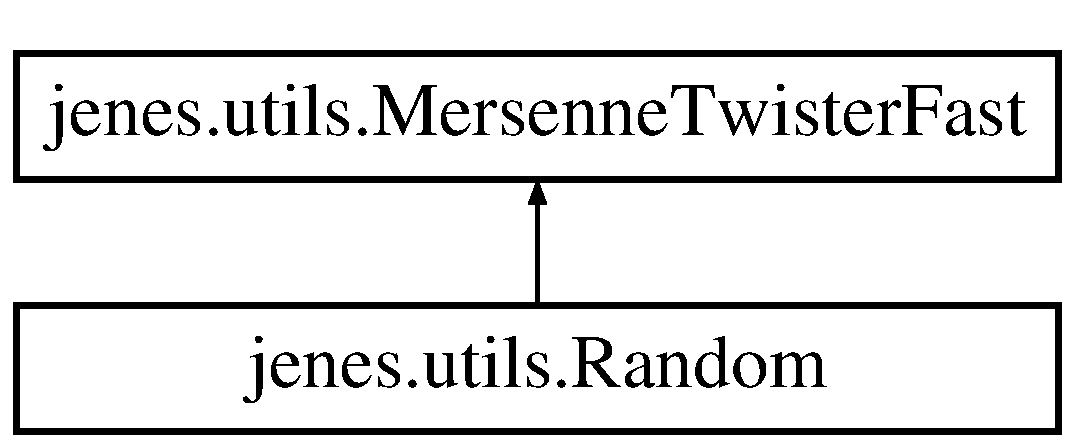
\includegraphics[height=2cm]{classjenes_1_1utils_1_1_mersenne_twister_fast}
\end{center}
\end{figure}
\subsection*{Public Member Functions}
\begin{CompactItemize}
\item 
\hyperlink{classjenes_1_1utils_1_1_mersenne_twister_fast_7321af0f92bcda7c245ebfbb647f7e4c}{MersenneTwisterFast} ()
\item 
\hyperlink{classjenes_1_1utils_1_1_mersenne_twister_fast_554aee5d390bb57ad30577b194c8b7b2}{MersenneTwisterFast} (final long seed)
\item 
final void \hyperlink{classjenes_1_1utils_1_1_mersenne_twister_fast_a44ca1bf8e9a2f272e248ea279f1e80c}{setSeed} (final long seed)
\item 
\hypertarget{classjenes_1_1utils_1_1_mersenne_twister_fast_063b45fa6e20a5eea9acbe45a8c48ce0}{
final int \textbf{nextInt} ()}
\label{classjenes_1_1utils_1_1_mersenne_twister_fast_063b45fa6e20a5eea9acbe45a8c48ce0}

\item 
\hypertarget{classjenes_1_1utils_1_1_mersenne_twister_fast_89d03c5b1815eff8c443ef081a869e78}{
final short \textbf{nextShort} ()}
\label{classjenes_1_1utils_1_1_mersenne_twister_fast_89d03c5b1815eff8c443ef081a869e78}

\item 
\hypertarget{classjenes_1_1utils_1_1_mersenne_twister_fast_8f7cb8ea9832581729660f5c0346ee3a}{
final char \textbf{nextChar} ()}
\label{classjenes_1_1utils_1_1_mersenne_twister_fast_8f7cb8ea9832581729660f5c0346ee3a}

\item 
\hypertarget{classjenes_1_1utils_1_1_mersenne_twister_fast_54fa48ab055886a90aefdcb816257f4b}{
final boolean \textbf{nextBoolean} ()}
\label{classjenes_1_1utils_1_1_mersenne_twister_fast_54fa48ab055886a90aefdcb816257f4b}

\item 
\hypertarget{classjenes_1_1utils_1_1_mersenne_twister_fast_5e7c0943fcc746a30277f0e09abbf60f}{
final byte \textbf{nextByte} ()}
\label{classjenes_1_1utils_1_1_mersenne_twister_fast_5e7c0943fcc746a30277f0e09abbf60f}

\item 
\hypertarget{classjenes_1_1utils_1_1_mersenne_twister_fast_237dc55841fd8bf544106d052833c374}{
final void \textbf{nextBytes} (final byte\mbox{[}$\,$\mbox{]} bytes)}
\label{classjenes_1_1utils_1_1_mersenne_twister_fast_237dc55841fd8bf544106d052833c374}

\item 
\hypertarget{classjenes_1_1utils_1_1_mersenne_twister_fast_1de4f36e5e4035569bbb79bb06d4e9c7}{
final long \textbf{nextLong} ()}
\label{classjenes_1_1utils_1_1_mersenne_twister_fast_1de4f36e5e4035569bbb79bb06d4e9c7}

\item 
final double \hyperlink{classjenes_1_1utils_1_1_mersenne_twister_fast_64238ab497c1e504c798355f682ea2b9}{nextDouble} ()
\item 
\hypertarget{classjenes_1_1utils_1_1_mersenne_twister_fast_4af0dd9a4366e476e4d45568cbb558e9}{
final double \textbf{nextGaussian} ()}
\label{classjenes_1_1utils_1_1_mersenne_twister_fast_4af0dd9a4366e476e4d45568cbb558e9}

\item 
\hypertarget{classjenes_1_1utils_1_1_mersenne_twister_fast_f2d30f1dec2a94ca26a3b1ccc0624ce9}{
final float \textbf{nextFloat} ()}
\label{classjenes_1_1utils_1_1_mersenne_twister_fast_f2d30f1dec2a94ca26a3b1ccc0624ce9}

\item 
final int \hyperlink{classjenes_1_1utils_1_1_mersenne_twister_fast_e66ea69e37e4866fbb3beecb4e66577a}{nextInt} (final int n)
\end{CompactItemize}
\subsection*{Static Public Member Functions}
\begin{CompactItemize}
\item 
static void \hyperlink{classjenes_1_1utils_1_1_mersenne_twister_fast_5c955ea4cf1b925290dd92ddecc0c510}{main} (String args\mbox{[}$\,$\mbox{]})
\end{CompactItemize}
\subsection*{Protected Member Functions}
\begin{CompactItemize}
\item 
long \hyperlink{classjenes_1_1utils_1_1_mersenne_twister_fast_88963c0469e0bad7a1834469cf0f7a10}{getSeed} ()
\end{CompactItemize}


\subsection{Detailed Description}
Mersenne Twister and \hyperlink{classjenes_1_1utils_1_1_mersenne_twister_fast}{MersenneTwisterFast}: 

{\bf \hyperlink{classjenes_1_1utils_1_1_mersenne_twister_fast}{MersenneTwisterFast}} is a drop-in subclass replacement for java.util.Random. It is properly synchronized and can be used in a multithreaded environment.

{\bf \hyperlink{classjenes_1_1utils_1_1_mersenne_twister_fast}{MersenneTwisterFast}} is not a subclass of java.util.Random. It has the same public methods as \hyperlink{classjenes_1_1utils_1_1_random}{Random} does, however, and it is algorithmically identical to MersenneTwister. \hyperlink{classjenes_1_1utils_1_1_mersenne_twister_fast}{MersenneTwisterFast} has hard-code inlined all of its methods directly, and made all of them final (well, the ones of consequence anyway). Further, these methods are {\em not\/} synchronized, so the same \hyperlink{classjenes_1_1utils_1_1_mersenne_twister_fast}{MersenneTwisterFast} instance cannot be shared by multiple threads. But all this helps \hyperlink{classjenes_1_1utils_1_1_mersenne_twister_fast}{MersenneTwisterFast} achieve over twice the speed of MersenneTwister.

{\bf About the Mersenne Twister. } This is a Java version of the C-program for MT19937: Integer version. next(32) generates one pseudorandom unsigned integer (32bit)

which is uniformly distributed among 0 to 2$^\wedge$32-1 for each call. next(int bits) $>$$>$$>$'s by (32-bits) to get a value ranging between 0 and 2$^\wedge$bits-1 long inclusive; hope that's correct. setSeed(seed) set initial values to the working area of 624 words. For setSeed(seed), seed is any 32-bit integer {\bf except for 0}.

Orignally Coded by Takuji Nishimura, considering the suggestions by Topher Cooper and Marc Rieffel in July-Aug. 1997. More information can be found \href{http://www.math.keio.ac.jp/matumoto/emt.html}{\tt here. }

Translated to Java by Michael Lecuyer January 30, 1999 Copyright (C) 1999 Michael Lecuyer 

This library is free software; you can redistribute it and or

modify it under the terms of the GNU Library General Public License as published by the Free Software Foundation; either version 2 of the License, or (at your option) any later version. This library is distributed in the hope that it will be useful,

but WITHOUT ANY WARRANTY; without even the implied warranty of MERCHANTABILITY or FITNESS FOR A PARTICULAR PURPOSE. See the GNU Library General Public License for more details. You should have received a copy of the GNU Library General Public License along with this library; if not, write to the Free Foundation, Inc., 59 Temple Place, Suite 330, Boston, MA 02111-1307 USA 

Makoto Matsumoto and Takuji Nishimura, the original authors ask \char`\"{}When you use this, send an email to: \href{mailto:matumoto@math.keio.ac.jp}{\tt matumoto@math.keio.ac.jp} with an appropriate reference to your work\char`\"{} You might also point out this was a translation. 

{\bf Reference. } M. Matsumoto and T. Nishimura, \char`\"{}Mersenne Twister: A 623-Dimensionally Equidistributed Uniform Pseudo-Random Number Generator\char`\"{}, {\em ACM Transactions on Modeling and Computer Simulation,\/} Vol. 8, No. 1, January 1998, pp 3--30.

{\bf About this version. } This is a modification of the \href{http://www.theorem.com/java/index.htm#Mersenne}{\tt original code} made to conform to proper java.util.Random format by \href{http://www.cs.umd.edu/users/seanl/}{\tt Sean Luke,} August 7, 1999.

{\bf Bug Fixes. }This implementation implements the bug fixes made in Java 1.2's version of \hyperlink{classjenes_1_1utils_1_1_random}{Random}, which means it can be used with earlier versions of Java. See \href{http://www.javasoft.com/products/jdk/1.2/docs/api/java/util/Random.html}{\tt the JDK 1.2 java.util.Random documentation} for further documentation on the random-number generation contracts made. Additionally, there's an undocumented bug in the JDK java.util.Random.nextBytes() method, which this code fixes.

{\bf Important Note. } Just like java.util.Random, this generator accepts a long seed but doesn't use all of it. java.util.Random uses 48 bits. The Mersenne Twister instead uses 32 bits (int size). So it's best if your seed does not exceed the int range. 

\subsection{Constructor \& Destructor Documentation}
\hypertarget{classjenes_1_1utils_1_1_mersenne_twister_fast_7321af0f92bcda7c245ebfbb647f7e4c}{
\index{jenes::utils::MersenneTwisterFast@{jenes::utils::MersenneTwisterFast}!MersenneTwisterFast@{MersenneTwisterFast}}
\index{MersenneTwisterFast@{MersenneTwisterFast}!jenes::utils::MersenneTwisterFast@{jenes::utils::MersenneTwisterFast}}
\subsubsection[MersenneTwisterFast]{\setlength{\rightskip}{0pt plus 5cm}jenes.utils.MersenneTwisterFast.MersenneTwisterFast ()}}
\label{classjenes_1_1utils_1_1_mersenne_twister_fast_7321af0f92bcda7c245ebfbb647f7e4c}


Constructor using the default seed. \hypertarget{classjenes_1_1utils_1_1_mersenne_twister_fast_554aee5d390bb57ad30577b194c8b7b2}{
\index{jenes::utils::MersenneTwisterFast@{jenes::utils::MersenneTwisterFast}!MersenneTwisterFast@{MersenneTwisterFast}}
\index{MersenneTwisterFast@{MersenneTwisterFast}!jenes::utils::MersenneTwisterFast@{jenes::utils::MersenneTwisterFast}}
\subsubsection[MersenneTwisterFast]{\setlength{\rightskip}{0pt plus 5cm}jenes.utils.MersenneTwisterFast.MersenneTwisterFast (final long {\em seed})}}
\label{classjenes_1_1utils_1_1_mersenne_twister_fast_554aee5d390bb57ad30577b194c8b7b2}


Constructor using a given seed. Though you pass this seed in as a long, it's best to make sure it's actually an integer.

\begin{Desc}
\item[Parameters:]
\begin{description}
\item[{\em seed}]generator starting number, often the time of day. \end{description}
\end{Desc}


\subsection{Member Function Documentation}
\hypertarget{classjenes_1_1utils_1_1_mersenne_twister_fast_a44ca1bf8e9a2f272e248ea279f1e80c}{
\index{jenes::utils::MersenneTwisterFast@{jenes::utils::MersenneTwisterFast}!setSeed@{setSeed}}
\index{setSeed@{setSeed}!jenes::utils::MersenneTwisterFast@{jenes::utils::MersenneTwisterFast}}
\subsubsection[setSeed]{\setlength{\rightskip}{0pt plus 5cm}final void jenes.utils.MersenneTwisterFast.setSeed (final long {\em seed})}}
\label{classjenes_1_1utils_1_1_mersenne_twister_fast_a44ca1bf8e9a2f272e248ea279f1e80c}


Initalize the pseudo random number generator. The Mersenne Twister only uses an integer for its seed; It's best that you don't pass in a long that's bigger than an int.

\begin{Desc}
\item[Parameters:]
\begin{description}
\item[{\em seed}]from constructor \end{description}
\end{Desc}
\hypertarget{classjenes_1_1utils_1_1_mersenne_twister_fast_88963c0469e0bad7a1834469cf0f7a10}{
\index{jenes::utils::MersenneTwisterFast@{jenes::utils::MersenneTwisterFast}!getSeed@{getSeed}}
\index{getSeed@{getSeed}!jenes::utils::MersenneTwisterFast@{jenes::utils::MersenneTwisterFast}}
\subsubsection[getSeed]{\setlength{\rightskip}{0pt plus 5cm}long jenes.utils.MersenneTwisterFast.getSeed ()\hspace{0.3cm}{\tt  \mbox{[}protected\mbox{]}}}}
\label{classjenes_1_1utils_1_1_mersenne_twister_fast_88963c0469e0bad7a1834469cf0f7a10}


Return the current used seed for random generator \begin{Desc}
\item[Returns:]\end{Desc}


Reimplemented in \hyperlink{classjenes_1_1utils_1_1_random_55f9b0a836c137e520658f55ad806859}{jenes.utils.Random}.\hypertarget{classjenes_1_1utils_1_1_mersenne_twister_fast_64238ab497c1e504c798355f682ea2b9}{
\index{jenes::utils::MersenneTwisterFast@{jenes::utils::MersenneTwisterFast}!nextDouble@{nextDouble}}
\index{nextDouble@{nextDouble}!jenes::utils::MersenneTwisterFast@{jenes::utils::MersenneTwisterFast}}
\subsubsection[nextDouble]{\setlength{\rightskip}{0pt plus 5cm}final double jenes.utils.MersenneTwisterFast.nextDouble ()}}
\label{classjenes_1_1utils_1_1_mersenne_twister_fast_64238ab497c1e504c798355f682ea2b9}


Returns a double uniformly distributed within \mbox{[}0,1\mbox{[} 

\begin{Desc}
\item[Returns:]a random double value \end{Desc}
\hypertarget{classjenes_1_1utils_1_1_mersenne_twister_fast_e66ea69e37e4866fbb3beecb4e66577a}{
\index{jenes::utils::MersenneTwisterFast@{jenes::utils::MersenneTwisterFast}!nextInt@{nextInt}}
\index{nextInt@{nextInt}!jenes::utils::MersenneTwisterFast@{jenes::utils::MersenneTwisterFast}}
\subsubsection[nextInt]{\setlength{\rightskip}{0pt plus 5cm}final int jenes.utils.MersenneTwisterFast.nextInt (final int {\em n})}}
\label{classjenes_1_1utils_1_1_mersenne_twister_fast_e66ea69e37e4866fbb3beecb4e66577a}


Returns an integer drawn uniformly from 0 to n-1. Suffice it to say, n must be $>$ 0, or an IllegalArgumentException is raised. \hypertarget{classjenes_1_1utils_1_1_mersenne_twister_fast_5c955ea4cf1b925290dd92ddecc0c510}{
\index{jenes::utils::MersenneTwisterFast@{jenes::utils::MersenneTwisterFast}!main@{main}}
\index{main@{main}!jenes::utils::MersenneTwisterFast@{jenes::utils::MersenneTwisterFast}}
\subsubsection[main]{\setlength{\rightskip}{0pt plus 5cm}static void jenes.utils.MersenneTwisterFast.main (String {\em args}\mbox{[}$\,$\mbox{]})\hspace{0.3cm}{\tt  \mbox{[}static\mbox{]}}}}
\label{classjenes_1_1utils_1_1_mersenne_twister_fast_5c955ea4cf1b925290dd92ddecc0c510}


Tests the code. 

The documentation for this class was generated from the following file:\begin{CompactItemize}
\item 
src/jenes/utils/MersenneTwisterFast.java\end{CompactItemize}

\hypertarget{classjenes_1_1stage_1_1operator_1_1common_1_1_multi_niche_crowder_3_01_t_01extends_01_chromosome_01_4}{
\section{jenes.stage.operator.common.MultiNicheCrowder$<$ T extends Chromosome $>$ Class Reference}
\label{classjenes_1_1stage_1_1operator_1_1common_1_1_multi_niche_crowder_3_01_t_01extends_01_chromosome_01_4}\index{jenes::stage::operator::common::MultiNicheCrowder$<$ T extends Chromosome $>$@{jenes::stage::operator::common::MultiNicheCrowder$<$ T extends Chromosome $>$}}
}
Inherits jenes::stage::operator::Crowder$<$ T $>$.

\subsection*{Public Types}
\begin{CompactItemize}
\item 
enum \hyperlink{classjenes_1_1stage_1_1operator_1_1common_1_1_multi_niche_crowder_3_01_t_01extends_01_chromosome_01_4_1190dbbe875b99f6679f7b5deb68483b}{SelectionMethod} \{ \par
\textbf{ROULETTE}, 
\textbf{TOURNAMENT}, 
\textbf{ROULETTE}, 
\textbf{TOURNAMENT}, 
\par
\textbf{ROULETTE}, 
\textbf{TOURNAMENT}, 
\textbf{NONE}, 
\textbf{ROULETTE}, 
\par
\textbf{TOURNAMENT}, 
\textbf{ROULETTE}, 
\textbf{TOURNAMENT}
 \}
\item 
enum \hyperlink{classjenes_1_1stage_1_1operator_1_1common_1_1_multi_niche_crowder_3_01_t_01extends_01_chromosome_01_4_273881bd444aeae8ef77816000eac94c}{CrossoverMethod} \{ \par
\textbf{SINGLEPOINT}, 
\textbf{TWOPOINTS}, 
\textbf{SINGLEPOINT}, 
\textbf{TWOPOINTS}, 
\par
\textbf{SINGLEPOINT}, 
\textbf{TWOPOINTS}, 
\textbf{SINGLEPOINT}, 
\textbf{TWOPOINTS}
 \}
\item 
enum \hyperlink{classjenes_1_1stage_1_1operator_1_1common_1_1_multi_niche_crowder_3_01_t_01extends_01_chromosome_01_4_1ea23e3abc5ae7417a422840824bab65}{MutationMethod} \{ \par
\textbf{NONE}, 
\textbf{SIMPLE}, 
\textbf{NONE}, 
\textbf{SIMPLE}, 
\par
\textbf{NONE}, 
\textbf{SIMPLE}
 \}
\end{CompactItemize}
\subsection*{Public Member Functions}
\begin{CompactItemize}
\item 
\hyperlink{classjenes_1_1stage_1_1operator_1_1common_1_1_multi_niche_crowder_3_01_t_01extends_01_chromosome_01_4_0e3210ea1f2d3f1687f5c1f9a0f326dd}{MultiNicheCrowder} ()
\item 
\hyperlink{classjenes_1_1stage_1_1operator_1_1common_1_1_multi_niche_crowder_3_01_t_01extends_01_chromosome_01_4_45d8181936a9298ecc7edcfee8647590}{MultiNicheCrowder} (final \hyperlink{classjenes_1_1stage_1_1operator_1_1common_1_1_multi_niche_crowder_3_01_t_01extends_01_chromosome_01_4_1190dbbe875b99f6679f7b5deb68483b}{SelectionMethod} selection)
\item 
\hyperlink{classjenes_1_1stage_1_1operator_1_1common_1_1_multi_niche_crowder_3_01_t_01extends_01_chromosome_01_4_5f539242ac756ac79df20945afc5e425}{MultiNicheCrowder} (final \hyperlink{classjenes_1_1stage_1_1operator_1_1common_1_1_multi_niche_crowder_3_01_t_01extends_01_chromosome_01_4_1190dbbe875b99f6679f7b5deb68483b}{SelectionMethod} selection, final \hyperlink{classjenes_1_1stage_1_1operator_1_1common_1_1_multi_niche_crowder_3_01_t_01extends_01_chromosome_01_4_273881bd444aeae8ef77816000eac94c}{CrossoverMethod} crossmethod)
\item 
\hyperlink{classjenes_1_1stage_1_1operator_1_1common_1_1_multi_niche_crowder_3_01_t_01extends_01_chromosome_01_4_d6b691057f10397e80669b101c7f437a}{MultiNicheCrowder} (final \hyperlink{classjenes_1_1stage_1_1operator_1_1common_1_1_multi_niche_crowder_3_01_t_01extends_01_chromosome_01_4_1190dbbe875b99f6679f7b5deb68483b}{SelectionMethod} selection, final \hyperlink{classjenes_1_1stage_1_1operator_1_1common_1_1_multi_niche_crowder_3_01_t_01extends_01_chromosome_01_4_273881bd444aeae8ef77816000eac94c}{CrossoverMethod} crossmethod, final double \hyperlink{classjenes_1_1stage_1_1operator_1_1common_1_1_multi_niche_crowder_3_01_t_01extends_01_chromosome_01_4_d584be099b23576ec3379a6867d31ef4}{crossover}, final double mutation)
\item 
\hyperlink{classjenes_1_1stage_1_1operator_1_1common_1_1_multi_niche_crowder_3_01_t_01extends_01_chromosome_01_4_7384c823b16fe8e5f8bfdc7db0c87ce5}{MultiNicheCrowder} (final \hyperlink{classjenes_1_1stage_1_1operator_1_1common_1_1_multi_niche_crowder_3_01_t_01extends_01_chromosome_01_4_1190dbbe875b99f6679f7b5deb68483b}{SelectionMethod} selectionmethod, final \hyperlink{classjenes_1_1stage_1_1operator_1_1common_1_1_multi_niche_crowder_3_01_t_01extends_01_chromosome_01_4_273881bd444aeae8ef77816000eac94c}{CrossoverMethod} crossmethod, final double \hyperlink{classjenes_1_1stage_1_1operator_1_1common_1_1_multi_niche_crowder_3_01_t_01extends_01_chromosome_01_4_d584be099b23576ec3379a6867d31ef4}{crossover}, final double mutation, final int sf, final int cf, final int rf)
\item 
final int \hyperlink{classjenes_1_1stage_1_1operator_1_1common_1_1_multi_niche_crowder_3_01_t_01extends_01_chromosome_01_4_74363393b7e200fcff467ff5920e10d6}{getCrowdingFactor} ()
\item 
void \hyperlink{classjenes_1_1stage_1_1operator_1_1common_1_1_multi_niche_crowder_3_01_t_01extends_01_chromosome_01_4_d00602ac8b97b385a8a72fd612e2ac22}{setCrowdingFactor} (int \hyperlink{classjenes_1_1stage_1_1operator_1_1common_1_1_multi_niche_crowder_3_01_t_01extends_01_chromosome_01_4_d7320907a72bd19c028f922383667560}{crowdingFactor})
\item 
final int \hyperlink{classjenes_1_1stage_1_1operator_1_1common_1_1_multi_niche_crowder_3_01_t_01extends_01_chromosome_01_4_97c2ba03c48234566aea9fcf49b677ee}{getReplacementFactor} ()
\item 
void \hyperlink{classjenes_1_1stage_1_1operator_1_1common_1_1_multi_niche_crowder_3_01_t_01extends_01_chromosome_01_4_3cf07082299cbe94d975a9af638a2098}{setReplacementFactor} (int \hyperlink{classjenes_1_1stage_1_1operator_1_1common_1_1_multi_niche_crowder_3_01_t_01extends_01_chromosome_01_4_9a068eae86d3af67f89cfa4b244810fb}{replacementFactor})
\item 
final int \hyperlink{classjenes_1_1stage_1_1operator_1_1common_1_1_multi_niche_crowder_3_01_t_01extends_01_chromosome_01_4_42e85f954b23bdadf63b7aa13365cd40}{getSelectionFactor} ()
\item 
void \hyperlink{classjenes_1_1stage_1_1operator_1_1common_1_1_multi_niche_crowder_3_01_t_01extends_01_chromosome_01_4_0f2ec39933d9656c981f8b7113bbf668}{setSelectionFactor} (int \hyperlink{classjenes_1_1stage_1_1operator_1_1common_1_1_multi_niche_crowder_3_01_t_01extends_01_chromosome_01_4_b561927a8af185e69bd5fcf85e904d7a}{selectionFactor})
\end{CompactItemize}
\subsection*{Static Public Attributes}
\begin{CompactItemize}
\item 
static final \hyperlink{classjenes_1_1stage_1_1operator_1_1common_1_1_multi_niche_crowder_3_01_t_01extends_01_chromosome_01_4_1190dbbe875b99f6679f7b5deb68483b}{SelectionMethod} \hyperlink{classjenes_1_1stage_1_1operator_1_1common_1_1_multi_niche_crowder_3_01_t_01extends_01_chromosome_01_4_ddd3f5fe352248ed9d5639e0d138f59d}{DEFAULT\_\-SELECTION\_\-METHOD} = SelectionMethod.TOURNAMENT
\item 
static final \hyperlink{classjenes_1_1stage_1_1operator_1_1common_1_1_multi_niche_crowder_3_01_t_01extends_01_chromosome_01_4_273881bd444aeae8ef77816000eac94c}{CrossoverMethod} \hyperlink{classjenes_1_1stage_1_1operator_1_1common_1_1_multi_niche_crowder_3_01_t_01extends_01_chromosome_01_4_ed986ca7d89144f78e73a11a5fb2f032}{DEFAULT\_\-CROSSOVER\_\-METHOD} = CrossoverMethod.SINGLEPOINT
\item 
static final double \hyperlink{classjenes_1_1stage_1_1operator_1_1common_1_1_multi_niche_crowder_3_01_t_01extends_01_chromosome_01_4_6e6d3f4e8201a341f77ac92954dbdad4}{DEFAULT\_\-CROSSOVER\_\-PROBABILITY} = 0.8
\item 
static final double \hyperlink{classjenes_1_1stage_1_1operator_1_1common_1_1_multi_niche_crowder_3_01_t_01extends_01_chromosome_01_4_a3cfe11747630124e10809b0027d6f3a}{DEFAULT\_\-MUTATION\_\-PROBABILITY} = 0.02
\item 
static final int \hyperlink{classjenes_1_1stage_1_1operator_1_1common_1_1_multi_niche_crowder_3_01_t_01extends_01_chromosome_01_4_937e501fc953576f30be99a0eec9ccf4}{DEFAULT\_\-SELECTION\_\-FACTOR} = 5
\item 
static final int \hyperlink{classjenes_1_1stage_1_1operator_1_1common_1_1_multi_niche_crowder_3_01_t_01extends_01_chromosome_01_4_e7c682fcbb8e1de5270d79ca482bd93d}{DEFAULT\_\-CROWDING\_\-FACTOR} = 5
\item 
static final int \hyperlink{classjenes_1_1stage_1_1operator_1_1common_1_1_multi_niche_crowder_3_01_t_01extends_01_chromosome_01_4_c38d4afc42b5f54473834e76815c7510}{DEFAULT\_\-REPLACEMENT\_\-FACTOR} = 5
\end{CompactItemize}
\subsection*{Protected Member Functions}
\begin{CompactItemize}
\item 
\hypertarget{classjenes_1_1stage_1_1operator_1_1common_1_1_multi_niche_crowder_3_01_t_01extends_01_chromosome_01_4_e3e96b6cd96f375209e9308bb7f9ca85}{
void \textbf{preselect} (Population$<$ T $>$ in, Population$<$ T $>$ out)}
\label{classjenes_1_1stage_1_1operator_1_1common_1_1_multi_niche_crowder_3_01_t_01extends_01_chromosome_01_4_e3e96b6cd96f375209e9308bb7f9ca85}

\item 
\hypertarget{classjenes_1_1stage_1_1operator_1_1common_1_1_multi_niche_crowder_3_01_t_01extends_01_chromosome_01_4_619884821dabf179aed435269366114e}{
void \textbf{replace} (Population$<$ T $>$ initial, Population$<$ T $>$ preselected, Population$<$ T $>$ evolved, Population$<$ T $>$ out)}
\label{classjenes_1_1stage_1_1operator_1_1common_1_1_multi_niche_crowder_3_01_t_01extends_01_chromosome_01_4_619884821dabf179aed435269366114e}

\end{CompactItemize}
\subsection*{Protected Attributes}
\begin{CompactItemize}
\item 
int \hyperlink{classjenes_1_1stage_1_1operator_1_1common_1_1_multi_niche_crowder_3_01_t_01extends_01_chromosome_01_4_b561927a8af185e69bd5fcf85e904d7a}{selectionFactor}
\item 
int \hyperlink{classjenes_1_1stage_1_1operator_1_1common_1_1_multi_niche_crowder_3_01_t_01extends_01_chromosome_01_4_d7320907a72bd19c028f922383667560}{crowdingFactor}
\item 
int \hyperlink{classjenes_1_1stage_1_1operator_1_1common_1_1_multi_niche_crowder_3_01_t_01extends_01_chromosome_01_4_9a068eae86d3af67f89cfa4b244810fb}{replacementFactor}
\item 
Crossover$<$ T $>$ \hyperlink{classjenes_1_1stage_1_1operator_1_1common_1_1_multi_niche_crowder_3_01_t_01extends_01_chromosome_01_4_d584be099b23576ec3379a6867d31ef4}{crossover}
\item 
Selector$<$ T $>$ \hyperlink{classjenes_1_1stage_1_1operator_1_1common_1_1_multi_niche_crowder_3_01_t_01extends_01_chromosome_01_4_ec9f82fc79b7a63f5e664dfbcc7e9563}{selector}
\end{CompactItemize}


\subsection{Detailed Description}
Implementation of multi-niche crowding.

\begin{Desc}
\item[Version:]2.0 \end{Desc}
\begin{Desc}
\item[Since:]2.0 \end{Desc}


\subsection{Member Enumeration Documentation}
\hypertarget{classjenes_1_1stage_1_1operator_1_1common_1_1_multi_niche_crowder_3_01_t_01extends_01_chromosome_01_4_1190dbbe875b99f6679f7b5deb68483b}{
\index{jenes::stage::operator::common::MultiNicheCrowder$<$ T extends Chromosome $>$@{jenes::stage::operator::common::MultiNicheCrowder$<$ T extends Chromosome $>$}!SelectionMethod@{SelectionMethod}}
\index{SelectionMethod@{SelectionMethod}!jenes::stage::operator::common::MultiNicheCrowder< T extends Chromosome >@{jenes::stage::operator::common::MultiNicheCrowder$<$ T extends Chromosome $>$}}
\subsubsection[SelectionMethod]{\setlength{\rightskip}{0pt plus 5cm}enum jenes::stage::operator::common::MultiNicheCrowder$<$ T extends Chromosome $>$::{\bf SelectionMethod}}}
\label{classjenes_1_1stage_1_1operator_1_1common_1_1_multi_niche_crowder_3_01_t_01extends_01_chromosome_01_4_1190dbbe875b99f6679f7b5deb68483b}


Provides the available selection methods \hypertarget{classjenes_1_1stage_1_1operator_1_1common_1_1_multi_niche_crowder_3_01_t_01extends_01_chromosome_01_4_273881bd444aeae8ef77816000eac94c}{
\index{jenes::stage::operator::common::MultiNicheCrowder$<$ T extends Chromosome $>$@{jenes::stage::operator::common::MultiNicheCrowder$<$ T extends Chromosome $>$}!CrossoverMethod@{CrossoverMethod}}
\index{CrossoverMethod@{CrossoverMethod}!jenes::stage::operator::common::MultiNicheCrowder< T extends Chromosome >@{jenes::stage::operator::common::MultiNicheCrowder$<$ T extends Chromosome $>$}}
\subsubsection[CrossoverMethod]{\setlength{\rightskip}{0pt plus 5cm}enum jenes::stage::operator::common::MultiNicheCrowder$<$ T extends Chromosome $>$::{\bf CrossoverMethod}}}
\label{classjenes_1_1stage_1_1operator_1_1common_1_1_multi_niche_crowder_3_01_t_01extends_01_chromosome_01_4_273881bd444aeae8ef77816000eac94c}


Provides the available crossover methods \hypertarget{classjenes_1_1stage_1_1operator_1_1common_1_1_multi_niche_crowder_3_01_t_01extends_01_chromosome_01_4_1ea23e3abc5ae7417a422840824bab65}{
\index{jenes::stage::operator::common::MultiNicheCrowder$<$ T extends Chromosome $>$@{jenes::stage::operator::common::MultiNicheCrowder$<$ T extends Chromosome $>$}!MutationMethod@{MutationMethod}}
\index{MutationMethod@{MutationMethod}!jenes::stage::operator::common::MultiNicheCrowder< T extends Chromosome >@{jenes::stage::operator::common::MultiNicheCrowder$<$ T extends Chromosome $>$}}
\subsubsection[MutationMethod]{\setlength{\rightskip}{0pt plus 5cm}enum jenes::stage::operator::common::MultiNicheCrowder$<$ T extends Chromosome $>$::{\bf MutationMethod}}}
\label{classjenes_1_1stage_1_1operator_1_1common_1_1_multi_niche_crowder_3_01_t_01extends_01_chromosome_01_4_1ea23e3abc5ae7417a422840824bab65}


Provides standard mutation methods 

\subsection{Constructor \& Destructor Documentation}
\hypertarget{classjenes_1_1stage_1_1operator_1_1common_1_1_multi_niche_crowder_3_01_t_01extends_01_chromosome_01_4_0e3210ea1f2d3f1687f5c1f9a0f326dd}{
\index{jenes::stage::operator::common::MultiNicheCrowder$<$ T extends Chromosome $>$@{jenes::stage::operator::common::MultiNicheCrowder$<$ T extends Chromosome $>$}!MultiNicheCrowder@{MultiNicheCrowder}}
\index{MultiNicheCrowder@{MultiNicheCrowder}!jenes::stage::operator::common::MultiNicheCrowder< T extends Chromosome >@{jenes::stage::operator::common::MultiNicheCrowder$<$ T extends Chromosome $>$}}
\subsubsection[MultiNicheCrowder]{\setlength{\rightskip}{0pt plus 5cm}jenes.stage.operator.common.MultiNicheCrowder$<$ T extends Chromosome $>$.MultiNicheCrowder ()}}
\label{classjenes_1_1stage_1_1operator_1_1common_1_1_multi_niche_crowder_3_01_t_01extends_01_chromosome_01_4_0e3210ea1f2d3f1687f5c1f9a0f326dd}


Creates MultiNicheCrowder using default options. \hypertarget{classjenes_1_1stage_1_1operator_1_1common_1_1_multi_niche_crowder_3_01_t_01extends_01_chromosome_01_4_45d8181936a9298ecc7edcfee8647590}{
\index{jenes::stage::operator::common::MultiNicheCrowder$<$ T extends Chromosome $>$@{jenes::stage::operator::common::MultiNicheCrowder$<$ T extends Chromosome $>$}!MultiNicheCrowder@{MultiNicheCrowder}}
\index{MultiNicheCrowder@{MultiNicheCrowder}!jenes::stage::operator::common::MultiNicheCrowder< T extends Chromosome >@{jenes::stage::operator::common::MultiNicheCrowder$<$ T extends Chromosome $>$}}
\subsubsection[MultiNicheCrowder]{\setlength{\rightskip}{0pt plus 5cm}jenes.stage.operator.common.MultiNicheCrowder$<$ T extends Chromosome $>$.MultiNicheCrowder (final {\bf SelectionMethod} {\em selection})}}
\label{classjenes_1_1stage_1_1operator_1_1common_1_1_multi_niche_crowder_3_01_t_01extends_01_chromosome_01_4_45d8181936a9298ecc7edcfee8647590}


Creates a MultiNicheCrowder instance

\begin{Desc}
\item[Parameters:]
\begin{description}
\item[{\em crossmethod}]crossover method \end{description}
\end{Desc}
\hypertarget{classjenes_1_1stage_1_1operator_1_1common_1_1_multi_niche_crowder_3_01_t_01extends_01_chromosome_01_4_5f539242ac756ac79df20945afc5e425}{
\index{jenes::stage::operator::common::MultiNicheCrowder$<$ T extends Chromosome $>$@{jenes::stage::operator::common::MultiNicheCrowder$<$ T extends Chromosome $>$}!MultiNicheCrowder@{MultiNicheCrowder}}
\index{MultiNicheCrowder@{MultiNicheCrowder}!jenes::stage::operator::common::MultiNicheCrowder< T extends Chromosome >@{jenes::stage::operator::common::MultiNicheCrowder$<$ T extends Chromosome $>$}}
\subsubsection[MultiNicheCrowder]{\setlength{\rightskip}{0pt plus 5cm}jenes.stage.operator.common.MultiNicheCrowder$<$ T extends Chromosome $>$.MultiNicheCrowder (final {\bf SelectionMethod} {\em selection}, \/  final {\bf CrossoverMethod} {\em crossmethod})}}
\label{classjenes_1_1stage_1_1operator_1_1common_1_1_multi_niche_crowder_3_01_t_01extends_01_chromosome_01_4_5f539242ac756ac79df20945afc5e425}


Creates a MultiNicheCrowder instance

\begin{Desc}
\item[Parameters:]
\begin{description}
\item[{\em crossmethod}]crossover method \end{description}
\end{Desc}
\hypertarget{classjenes_1_1stage_1_1operator_1_1common_1_1_multi_niche_crowder_3_01_t_01extends_01_chromosome_01_4_d6b691057f10397e80669b101c7f437a}{
\index{jenes::stage::operator::common::MultiNicheCrowder$<$ T extends Chromosome $>$@{jenes::stage::operator::common::MultiNicheCrowder$<$ T extends Chromosome $>$}!MultiNicheCrowder@{MultiNicheCrowder}}
\index{MultiNicheCrowder@{MultiNicheCrowder}!jenes::stage::operator::common::MultiNicheCrowder< T extends Chromosome >@{jenes::stage::operator::common::MultiNicheCrowder$<$ T extends Chromosome $>$}}
\subsubsection[MultiNicheCrowder]{\setlength{\rightskip}{0pt plus 5cm}jenes.stage.operator.common.MultiNicheCrowder$<$ T extends Chromosome $>$.MultiNicheCrowder (final {\bf SelectionMethod} {\em selection}, \/  final {\bf CrossoverMethod} {\em crossmethod}, \/  final double {\em crossover}, \/  final double {\em mutation})}}
\label{classjenes_1_1stage_1_1operator_1_1common_1_1_multi_niche_crowder_3_01_t_01extends_01_chromosome_01_4_d6b691057f10397e80669b101c7f437a}


Creates a MultiNicheCrowder instance

\begin{Desc}
\item[Parameters:]
\begin{description}
\item[{\em crossmethod}]crossover method \item[{\em crossover}]crossover probability \item[{\em mutation}]mutation probability \end{description}
\end{Desc}
\hypertarget{classjenes_1_1stage_1_1operator_1_1common_1_1_multi_niche_crowder_3_01_t_01extends_01_chromosome_01_4_7384c823b16fe8e5f8bfdc7db0c87ce5}{
\index{jenes::stage::operator::common::MultiNicheCrowder$<$ T extends Chromosome $>$@{jenes::stage::operator::common::MultiNicheCrowder$<$ T extends Chromosome $>$}!MultiNicheCrowder@{MultiNicheCrowder}}
\index{MultiNicheCrowder@{MultiNicheCrowder}!jenes::stage::operator::common::MultiNicheCrowder< T extends Chromosome >@{jenes::stage::operator::common::MultiNicheCrowder$<$ T extends Chromosome $>$}}
\subsubsection[MultiNicheCrowder]{\setlength{\rightskip}{0pt plus 5cm}jenes.stage.operator.common.MultiNicheCrowder$<$ T extends Chromosome $>$.MultiNicheCrowder (final {\bf SelectionMethod} {\em selectionmethod}, \/  final {\bf CrossoverMethod} {\em crossmethod}, \/  final double {\em crossover}, \/  final double {\em mutation}, \/  final int {\em sf}, \/  final int {\em cf}, \/  final int {\em rf})}}
\label{classjenes_1_1stage_1_1operator_1_1common_1_1_multi_niche_crowder_3_01_t_01extends_01_chromosome_01_4_7384c823b16fe8e5f8bfdc7db0c87ce5}


Creates a MultiNicheCrowder instance

\begin{Desc}
\item[Parameters:]
\begin{description}
\item[{\em crossmethod}]crossover method \item[{\em crossover}]crossover probability \item[{\em mutation}]mutation probability \item[{\em sf}]selection factor \item[{\em cf}]crowding factor \item[{\em rf}]replacement factor \end{description}
\end{Desc}


\subsection{Member Function Documentation}
\hypertarget{classjenes_1_1stage_1_1operator_1_1common_1_1_multi_niche_crowder_3_01_t_01extends_01_chromosome_01_4_74363393b7e200fcff467ff5920e10d6}{
\index{jenes::stage::operator::common::MultiNicheCrowder$<$ T extends Chromosome $>$@{jenes::stage::operator::common::MultiNicheCrowder$<$ T extends Chromosome $>$}!getCrowdingFactor@{getCrowdingFactor}}
\index{getCrowdingFactor@{getCrowdingFactor}!jenes::stage::operator::common::MultiNicheCrowder< T extends Chromosome >@{jenes::stage::operator::common::MultiNicheCrowder$<$ T extends Chromosome $>$}}
\subsubsection[getCrowdingFactor]{\setlength{\rightskip}{0pt plus 5cm}final int jenes.stage.operator.common.MultiNicheCrowder$<$ T extends Chromosome $>$.getCrowdingFactor ()}}
\label{classjenes_1_1stage_1_1operator_1_1common_1_1_multi_niche_crowder_3_01_t_01extends_01_chromosome_01_4_74363393b7e200fcff467ff5920e10d6}


Returns the crowding factor

\begin{Desc}
\item[Returns:]\end{Desc}
\hypertarget{classjenes_1_1stage_1_1operator_1_1common_1_1_multi_niche_crowder_3_01_t_01extends_01_chromosome_01_4_d00602ac8b97b385a8a72fd612e2ac22}{
\index{jenes::stage::operator::common::MultiNicheCrowder$<$ T extends Chromosome $>$@{jenes::stage::operator::common::MultiNicheCrowder$<$ T extends Chromosome $>$}!setCrowdingFactor@{setCrowdingFactor}}
\index{setCrowdingFactor@{setCrowdingFactor}!jenes::stage::operator::common::MultiNicheCrowder< T extends Chromosome >@{jenes::stage::operator::common::MultiNicheCrowder$<$ T extends Chromosome $>$}}
\subsubsection[setCrowdingFactor]{\setlength{\rightskip}{0pt plus 5cm}void jenes.stage.operator.common.MultiNicheCrowder$<$ T extends Chromosome $>$.setCrowdingFactor (int {\em crowdingFactor})}}
\label{classjenes_1_1stage_1_1operator_1_1common_1_1_multi_niche_crowder_3_01_t_01extends_01_chromosome_01_4_d00602ac8b97b385a8a72fd612e2ac22}


Sets the crowding factor

\begin{Desc}
\item[Parameters:]
\begin{description}
\item[{\em crowdingFactor}]the factor \end{description}
\end{Desc}
\hypertarget{classjenes_1_1stage_1_1operator_1_1common_1_1_multi_niche_crowder_3_01_t_01extends_01_chromosome_01_4_97c2ba03c48234566aea9fcf49b677ee}{
\index{jenes::stage::operator::common::MultiNicheCrowder$<$ T extends Chromosome $>$@{jenes::stage::operator::common::MultiNicheCrowder$<$ T extends Chromosome $>$}!getReplacementFactor@{getReplacementFactor}}
\index{getReplacementFactor@{getReplacementFactor}!jenes::stage::operator::common::MultiNicheCrowder< T extends Chromosome >@{jenes::stage::operator::common::MultiNicheCrowder$<$ T extends Chromosome $>$}}
\subsubsection[getReplacementFactor]{\setlength{\rightskip}{0pt plus 5cm}final int jenes.stage.operator.common.MultiNicheCrowder$<$ T extends Chromosome $>$.getReplacementFactor ()}}
\label{classjenes_1_1stage_1_1operator_1_1common_1_1_multi_niche_crowder_3_01_t_01extends_01_chromosome_01_4_97c2ba03c48234566aea9fcf49b677ee}


Returns the replacement factor

\begin{Desc}
\item[Returns:]\end{Desc}
\hypertarget{classjenes_1_1stage_1_1operator_1_1common_1_1_multi_niche_crowder_3_01_t_01extends_01_chromosome_01_4_3cf07082299cbe94d975a9af638a2098}{
\index{jenes::stage::operator::common::MultiNicheCrowder$<$ T extends Chromosome $>$@{jenes::stage::operator::common::MultiNicheCrowder$<$ T extends Chromosome $>$}!setReplacementFactor@{setReplacementFactor}}
\index{setReplacementFactor@{setReplacementFactor}!jenes::stage::operator::common::MultiNicheCrowder< T extends Chromosome >@{jenes::stage::operator::common::MultiNicheCrowder$<$ T extends Chromosome $>$}}
\subsubsection[setReplacementFactor]{\setlength{\rightskip}{0pt plus 5cm}void jenes.stage.operator.common.MultiNicheCrowder$<$ T extends Chromosome $>$.setReplacementFactor (int {\em replacementFactor})}}
\label{classjenes_1_1stage_1_1operator_1_1common_1_1_multi_niche_crowder_3_01_t_01extends_01_chromosome_01_4_3cf07082299cbe94d975a9af638a2098}


Sets the replacement factor

\begin{Desc}
\item[Parameters:]
\begin{description}
\item[{\em replacementFactor}]the factor \end{description}
\end{Desc}
\hypertarget{classjenes_1_1stage_1_1operator_1_1common_1_1_multi_niche_crowder_3_01_t_01extends_01_chromosome_01_4_42e85f954b23bdadf63b7aa13365cd40}{
\index{jenes::stage::operator::common::MultiNicheCrowder$<$ T extends Chromosome $>$@{jenes::stage::operator::common::MultiNicheCrowder$<$ T extends Chromosome $>$}!getSelectionFactor@{getSelectionFactor}}
\index{getSelectionFactor@{getSelectionFactor}!jenes::stage::operator::common::MultiNicheCrowder< T extends Chromosome >@{jenes::stage::operator::common::MultiNicheCrowder$<$ T extends Chromosome $>$}}
\subsubsection[getSelectionFactor]{\setlength{\rightskip}{0pt plus 5cm}final int jenes.stage.operator.common.MultiNicheCrowder$<$ T extends Chromosome $>$.getSelectionFactor ()}}
\label{classjenes_1_1stage_1_1operator_1_1common_1_1_multi_niche_crowder_3_01_t_01extends_01_chromosome_01_4_42e85f954b23bdadf63b7aa13365cd40}


Return the selection factor

\begin{Desc}
\item[Returns:]\end{Desc}
\hypertarget{classjenes_1_1stage_1_1operator_1_1common_1_1_multi_niche_crowder_3_01_t_01extends_01_chromosome_01_4_0f2ec39933d9656c981f8b7113bbf668}{
\index{jenes::stage::operator::common::MultiNicheCrowder$<$ T extends Chromosome $>$@{jenes::stage::operator::common::MultiNicheCrowder$<$ T extends Chromosome $>$}!setSelectionFactor@{setSelectionFactor}}
\index{setSelectionFactor@{setSelectionFactor}!jenes::stage::operator::common::MultiNicheCrowder< T extends Chromosome >@{jenes::stage::operator::common::MultiNicheCrowder$<$ T extends Chromosome $>$}}
\subsubsection[setSelectionFactor]{\setlength{\rightskip}{0pt plus 5cm}void jenes.stage.operator.common.MultiNicheCrowder$<$ T extends Chromosome $>$.setSelectionFactor (int {\em selectionFactor})}}
\label{classjenes_1_1stage_1_1operator_1_1common_1_1_multi_niche_crowder_3_01_t_01extends_01_chromosome_01_4_0f2ec39933d9656c981f8b7113bbf668}


Sets the replacement factor

\begin{Desc}
\item[Parameters:]
\begin{description}
\item[{\em selectionFactor}]the factor \end{description}
\end{Desc}


\subsection{Member Data Documentation}
\hypertarget{classjenes_1_1stage_1_1operator_1_1common_1_1_multi_niche_crowder_3_01_t_01extends_01_chromosome_01_4_ddd3f5fe352248ed9d5639e0d138f59d}{
\index{jenes::stage::operator::common::MultiNicheCrowder$<$ T extends Chromosome $>$@{jenes::stage::operator::common::MultiNicheCrowder$<$ T extends Chromosome $>$}!DEFAULT\_\-SELECTION\_\-METHOD@{DEFAULT\_\-SELECTION\_\-METHOD}}
\index{DEFAULT\_\-SELECTION\_\-METHOD@{DEFAULT\_\-SELECTION\_\-METHOD}!jenes::stage::operator::common::MultiNicheCrowder< T extends Chromosome >@{jenes::stage::operator::common::MultiNicheCrowder$<$ T extends Chromosome $>$}}
\subsubsection[DEFAULT\_\-SELECTION\_\-METHOD]{\setlength{\rightskip}{0pt plus 5cm}final {\bf SelectionMethod} jenes.stage.operator.common.MultiNicheCrowder$<$ T extends Chromosome $>$.{\bf DEFAULT\_\-SELECTION\_\-METHOD} = SelectionMethod.TOURNAMENT\hspace{0.3cm}{\tt  \mbox{[}static\mbox{]}}}}
\label{classjenes_1_1stage_1_1operator_1_1common_1_1_multi_niche_crowder_3_01_t_01extends_01_chromosome_01_4_ddd3f5fe352248ed9d5639e0d138f59d}


The default selection method \hypertarget{classjenes_1_1stage_1_1operator_1_1common_1_1_multi_niche_crowder_3_01_t_01extends_01_chromosome_01_4_ed986ca7d89144f78e73a11a5fb2f032}{
\index{jenes::stage::operator::common::MultiNicheCrowder$<$ T extends Chromosome $>$@{jenes::stage::operator::common::MultiNicheCrowder$<$ T extends Chromosome $>$}!DEFAULT\_\-CROSSOVER\_\-METHOD@{DEFAULT\_\-CROSSOVER\_\-METHOD}}
\index{DEFAULT\_\-CROSSOVER\_\-METHOD@{DEFAULT\_\-CROSSOVER\_\-METHOD}!jenes::stage::operator::common::MultiNicheCrowder< T extends Chromosome >@{jenes::stage::operator::common::MultiNicheCrowder$<$ T extends Chromosome $>$}}
\subsubsection[DEFAULT\_\-CROSSOVER\_\-METHOD]{\setlength{\rightskip}{0pt plus 5cm}final {\bf CrossoverMethod} jenes.stage.operator.common.MultiNicheCrowder$<$ T extends Chromosome $>$.{\bf DEFAULT\_\-CROSSOVER\_\-METHOD} = CrossoverMethod.SINGLEPOINT\hspace{0.3cm}{\tt  \mbox{[}static\mbox{]}}}}
\label{classjenes_1_1stage_1_1operator_1_1common_1_1_multi_niche_crowder_3_01_t_01extends_01_chromosome_01_4_ed986ca7d89144f78e73a11a5fb2f032}


The default crossover method \hypertarget{classjenes_1_1stage_1_1operator_1_1common_1_1_multi_niche_crowder_3_01_t_01extends_01_chromosome_01_4_6e6d3f4e8201a341f77ac92954dbdad4}{
\index{jenes::stage::operator::common::MultiNicheCrowder$<$ T extends Chromosome $>$@{jenes::stage::operator::common::MultiNicheCrowder$<$ T extends Chromosome $>$}!DEFAULT\_\-CROSSOVER\_\-PROBABILITY@{DEFAULT\_\-CROSSOVER\_\-PROBABILITY}}
\index{DEFAULT\_\-CROSSOVER\_\-PROBABILITY@{DEFAULT\_\-CROSSOVER\_\-PROBABILITY}!jenes::stage::operator::common::MultiNicheCrowder< T extends Chromosome >@{jenes::stage::operator::common::MultiNicheCrowder$<$ T extends Chromosome $>$}}
\subsubsection[DEFAULT\_\-CROSSOVER\_\-PROBABILITY]{\setlength{\rightskip}{0pt plus 5cm}final double jenes.stage.operator.common.MultiNicheCrowder$<$ T extends Chromosome $>$.{\bf DEFAULT\_\-CROSSOVER\_\-PROBABILITY} = 0.8\hspace{0.3cm}{\tt  \mbox{[}static\mbox{]}}}}
\label{classjenes_1_1stage_1_1operator_1_1common_1_1_multi_niche_crowder_3_01_t_01extends_01_chromosome_01_4_6e6d3f4e8201a341f77ac92954dbdad4}


The default crossover probability \hypertarget{classjenes_1_1stage_1_1operator_1_1common_1_1_multi_niche_crowder_3_01_t_01extends_01_chromosome_01_4_a3cfe11747630124e10809b0027d6f3a}{
\index{jenes::stage::operator::common::MultiNicheCrowder$<$ T extends Chromosome $>$@{jenes::stage::operator::common::MultiNicheCrowder$<$ T extends Chromosome $>$}!DEFAULT\_\-MUTATION\_\-PROBABILITY@{DEFAULT\_\-MUTATION\_\-PROBABILITY}}
\index{DEFAULT\_\-MUTATION\_\-PROBABILITY@{DEFAULT\_\-MUTATION\_\-PROBABILITY}!jenes::stage::operator::common::MultiNicheCrowder< T extends Chromosome >@{jenes::stage::operator::common::MultiNicheCrowder$<$ T extends Chromosome $>$}}
\subsubsection[DEFAULT\_\-MUTATION\_\-PROBABILITY]{\setlength{\rightskip}{0pt plus 5cm}final double jenes.stage.operator.common.MultiNicheCrowder$<$ T extends Chromosome $>$.{\bf DEFAULT\_\-MUTATION\_\-PROBABILITY} = 0.02\hspace{0.3cm}{\tt  \mbox{[}static\mbox{]}}}}
\label{classjenes_1_1stage_1_1operator_1_1common_1_1_multi_niche_crowder_3_01_t_01extends_01_chromosome_01_4_a3cfe11747630124e10809b0027d6f3a}


The default mutation probability \hypertarget{classjenes_1_1stage_1_1operator_1_1common_1_1_multi_niche_crowder_3_01_t_01extends_01_chromosome_01_4_937e501fc953576f30be99a0eec9ccf4}{
\index{jenes::stage::operator::common::MultiNicheCrowder$<$ T extends Chromosome $>$@{jenes::stage::operator::common::MultiNicheCrowder$<$ T extends Chromosome $>$}!DEFAULT\_\-SELECTION\_\-FACTOR@{DEFAULT\_\-SELECTION\_\-FACTOR}}
\index{DEFAULT\_\-SELECTION\_\-FACTOR@{DEFAULT\_\-SELECTION\_\-FACTOR}!jenes::stage::operator::common::MultiNicheCrowder< T extends Chromosome >@{jenes::stage::operator::common::MultiNicheCrowder$<$ T extends Chromosome $>$}}
\subsubsection[DEFAULT\_\-SELECTION\_\-FACTOR]{\setlength{\rightskip}{0pt plus 5cm}final int jenes.stage.operator.common.MultiNicheCrowder$<$ T extends Chromosome $>$.{\bf DEFAULT\_\-SELECTION\_\-FACTOR} = 5\hspace{0.3cm}{\tt  \mbox{[}static\mbox{]}}}}
\label{classjenes_1_1stage_1_1operator_1_1common_1_1_multi_niche_crowder_3_01_t_01extends_01_chromosome_01_4_937e501fc953576f30be99a0eec9ccf4}


The default selection factor \hypertarget{classjenes_1_1stage_1_1operator_1_1common_1_1_multi_niche_crowder_3_01_t_01extends_01_chromosome_01_4_e7c682fcbb8e1de5270d79ca482bd93d}{
\index{jenes::stage::operator::common::MultiNicheCrowder$<$ T extends Chromosome $>$@{jenes::stage::operator::common::MultiNicheCrowder$<$ T extends Chromosome $>$}!DEFAULT\_\-CROWDING\_\-FACTOR@{DEFAULT\_\-CROWDING\_\-FACTOR}}
\index{DEFAULT\_\-CROWDING\_\-FACTOR@{DEFAULT\_\-CROWDING\_\-FACTOR}!jenes::stage::operator::common::MultiNicheCrowder< T extends Chromosome >@{jenes::stage::operator::common::MultiNicheCrowder$<$ T extends Chromosome $>$}}
\subsubsection[DEFAULT\_\-CROWDING\_\-FACTOR]{\setlength{\rightskip}{0pt plus 5cm}final int jenes.stage.operator.common.MultiNicheCrowder$<$ T extends Chromosome $>$.{\bf DEFAULT\_\-CROWDING\_\-FACTOR} = 5\hspace{0.3cm}{\tt  \mbox{[}static\mbox{]}}}}
\label{classjenes_1_1stage_1_1operator_1_1common_1_1_multi_niche_crowder_3_01_t_01extends_01_chromosome_01_4_e7c682fcbb8e1de5270d79ca482bd93d}


The default crowding factor \hypertarget{classjenes_1_1stage_1_1operator_1_1common_1_1_multi_niche_crowder_3_01_t_01extends_01_chromosome_01_4_c38d4afc42b5f54473834e76815c7510}{
\index{jenes::stage::operator::common::MultiNicheCrowder$<$ T extends Chromosome $>$@{jenes::stage::operator::common::MultiNicheCrowder$<$ T extends Chromosome $>$}!DEFAULT\_\-REPLACEMENT\_\-FACTOR@{DEFAULT\_\-REPLACEMENT\_\-FACTOR}}
\index{DEFAULT\_\-REPLACEMENT\_\-FACTOR@{DEFAULT\_\-REPLACEMENT\_\-FACTOR}!jenes::stage::operator::common::MultiNicheCrowder< T extends Chromosome >@{jenes::stage::operator::common::MultiNicheCrowder$<$ T extends Chromosome $>$}}
\subsubsection[DEFAULT\_\-REPLACEMENT\_\-FACTOR]{\setlength{\rightskip}{0pt plus 5cm}final int jenes.stage.operator.common.MultiNicheCrowder$<$ T extends Chromosome $>$.{\bf DEFAULT\_\-REPLACEMENT\_\-FACTOR} = 5\hspace{0.3cm}{\tt  \mbox{[}static\mbox{]}}}}
\label{classjenes_1_1stage_1_1operator_1_1common_1_1_multi_niche_crowder_3_01_t_01extends_01_chromosome_01_4_c38d4afc42b5f54473834e76815c7510}


The default replacement factor \hypertarget{classjenes_1_1stage_1_1operator_1_1common_1_1_multi_niche_crowder_3_01_t_01extends_01_chromosome_01_4_b561927a8af185e69bd5fcf85e904d7a}{
\index{jenes::stage::operator::common::MultiNicheCrowder$<$ T extends Chromosome $>$@{jenes::stage::operator::common::MultiNicheCrowder$<$ T extends Chromosome $>$}!selectionFactor@{selectionFactor}}
\index{selectionFactor@{selectionFactor}!jenes::stage::operator::common::MultiNicheCrowder< T extends Chromosome >@{jenes::stage::operator::common::MultiNicheCrowder$<$ T extends Chromosome $>$}}
\subsubsection[selectionFactor]{\setlength{\rightskip}{0pt plus 5cm}int jenes.stage.operator.common.MultiNicheCrowder$<$ T extends Chromosome $>$.{\bf selectionFactor}\hspace{0.3cm}{\tt  \mbox{[}protected\mbox{]}}}}
\label{classjenes_1_1stage_1_1operator_1_1common_1_1_multi_niche_crowder_3_01_t_01extends_01_chromosome_01_4_b561927a8af185e69bd5fcf85e904d7a}


Selection factor \hypertarget{classjenes_1_1stage_1_1operator_1_1common_1_1_multi_niche_crowder_3_01_t_01extends_01_chromosome_01_4_d7320907a72bd19c028f922383667560}{
\index{jenes::stage::operator::common::MultiNicheCrowder$<$ T extends Chromosome $>$@{jenes::stage::operator::common::MultiNicheCrowder$<$ T extends Chromosome $>$}!crowdingFactor@{crowdingFactor}}
\index{crowdingFactor@{crowdingFactor}!jenes::stage::operator::common::MultiNicheCrowder< T extends Chromosome >@{jenes::stage::operator::common::MultiNicheCrowder$<$ T extends Chromosome $>$}}
\subsubsection[crowdingFactor]{\setlength{\rightskip}{0pt plus 5cm}int jenes.stage.operator.common.MultiNicheCrowder$<$ T extends Chromosome $>$.{\bf crowdingFactor}\hspace{0.3cm}{\tt  \mbox{[}protected\mbox{]}}}}
\label{classjenes_1_1stage_1_1operator_1_1common_1_1_multi_niche_crowder_3_01_t_01extends_01_chromosome_01_4_d7320907a72bd19c028f922383667560}


Crowding factor \hypertarget{classjenes_1_1stage_1_1operator_1_1common_1_1_multi_niche_crowder_3_01_t_01extends_01_chromosome_01_4_9a068eae86d3af67f89cfa4b244810fb}{
\index{jenes::stage::operator::common::MultiNicheCrowder$<$ T extends Chromosome $>$@{jenes::stage::operator::common::MultiNicheCrowder$<$ T extends Chromosome $>$}!replacementFactor@{replacementFactor}}
\index{replacementFactor@{replacementFactor}!jenes::stage::operator::common::MultiNicheCrowder< T extends Chromosome >@{jenes::stage::operator::common::MultiNicheCrowder$<$ T extends Chromosome $>$}}
\subsubsection[replacementFactor]{\setlength{\rightskip}{0pt plus 5cm}int jenes.stage.operator.common.MultiNicheCrowder$<$ T extends Chromosome $>$.{\bf replacementFactor}\hspace{0.3cm}{\tt  \mbox{[}protected\mbox{]}}}}
\label{classjenes_1_1stage_1_1operator_1_1common_1_1_multi_niche_crowder_3_01_t_01extends_01_chromosome_01_4_9a068eae86d3af67f89cfa4b244810fb}


Replacement factor \hypertarget{classjenes_1_1stage_1_1operator_1_1common_1_1_multi_niche_crowder_3_01_t_01extends_01_chromosome_01_4_d584be099b23576ec3379a6867d31ef4}{
\index{jenes::stage::operator::common::MultiNicheCrowder$<$ T extends Chromosome $>$@{jenes::stage::operator::common::MultiNicheCrowder$<$ T extends Chromosome $>$}!crossover@{crossover}}
\index{crossover@{crossover}!jenes::stage::operator::common::MultiNicheCrowder< T extends Chromosome >@{jenes::stage::operator::common::MultiNicheCrowder$<$ T extends Chromosome $>$}}
\subsubsection[crossover]{\setlength{\rightskip}{0pt plus 5cm}Crossover$<$T$>$ jenes.stage.operator.common.MultiNicheCrowder$<$ T extends Chromosome $>$.{\bf crossover}\hspace{0.3cm}{\tt  \mbox{[}protected\mbox{]}}}}
\label{classjenes_1_1stage_1_1operator_1_1common_1_1_multi_niche_crowder_3_01_t_01extends_01_chromosome_01_4_d584be099b23576ec3379a6867d31ef4}


Crossover operator \hypertarget{classjenes_1_1stage_1_1operator_1_1common_1_1_multi_niche_crowder_3_01_t_01extends_01_chromosome_01_4_ec9f82fc79b7a63f5e664dfbcc7e9563}{
\index{jenes::stage::operator::common::MultiNicheCrowder$<$ T extends Chromosome $>$@{jenes::stage::operator::common::MultiNicheCrowder$<$ T extends Chromosome $>$}!selector@{selector}}
\index{selector@{selector}!jenes::stage::operator::common::MultiNicheCrowder< T extends Chromosome >@{jenes::stage::operator::common::MultiNicheCrowder$<$ T extends Chromosome $>$}}
\subsubsection[selector]{\setlength{\rightskip}{0pt plus 5cm}Selector$<$T$>$ jenes.stage.operator.common.MultiNicheCrowder$<$ T extends Chromosome $>$.{\bf selector}\hspace{0.3cm}{\tt  \mbox{[}protected\mbox{]}}}}
\label{classjenes_1_1stage_1_1operator_1_1common_1_1_multi_niche_crowder_3_01_t_01extends_01_chromosome_01_4_ec9f82fc79b7a63f5e664dfbcc7e9563}


Selector operator 

The documentation for this class was generated from the following file:\begin{CompactItemize}
\item 
src/jenes/stage/operator/common/MultiNicheCrowder.java\end{CompactItemize}

\hypertarget{classjenes_1_1tutorials_1_1old_1_1problem12_1_1_multi_objective_problem}{
\section{jenes.tutorials.old.problem12.MultiObjectiveProblem Class Reference}
\label{classjenes_1_1tutorials_1_1old_1_1problem12_1_1_multi_objective_problem}\index{jenes::tutorials::old::problem12::MultiObjectiveProblem@{jenes::tutorials::old::problem12::MultiObjectiveProblem}}
}
\subsection*{Static Public Member Functions}
\begin{CompactItemize}
\item 
\hypertarget{classjenes_1_1tutorials_1_1old_1_1problem12_1_1_multi_objective_problem_a56b8e189215e753714d1ed16fdf1075}{
static void \textbf{main} (String...args)  throws IOException }
\label{classjenes_1_1tutorials_1_1old_1_1problem12_1_1_multi_objective_problem_a56b8e189215e753714d1ed16fdf1075}

\item 
\hypertarget{classjenes_1_1tutorials_1_1old_1_1problem12_1_1_multi_objective_problem_793287d33c3ae22a258312881dbed2a3}{
static void \textbf{decode} (\hyperlink{classjenes_1_1tutorials_1_1old_1_1problem12_1_1_function}{Function} f, \hyperlink{classjenes_1_1chromosome_1_1_bitwise_chromosome}{BitwiseChromosome} chrom, double\mbox{[}$\,$\mbox{]} x)}
\label{classjenes_1_1tutorials_1_1old_1_1problem12_1_1_multi_objective_problem_793287d33c3ae22a258312881dbed2a3}

\end{CompactItemize}


\subsection{Detailed Description}
This tutorial represent an example of how to use multi-objective NSGA2 problem in Jenes. 

The documentation for this class was generated from the following file:\begin{CompactItemize}
\item 
src/jenes/tutorials/old/problem12/MultiObjectiveProblem.java\end{CompactItemize}

\hypertarget{classjenes_1_1utils_1_1multitasking_1_1_multi_thread_evaluator}{
\section{jenes.utils.multitasking.MultiThreadEvaluator Class Reference}
\label{classjenes_1_1utils_1_1multitasking_1_1_multi_thread_evaluator}\index{jenes::utils::multitasking::MultiThreadEvaluator@{jenes::utils::multitasking::MultiThreadEvaluator}}
}
Inheritance diagram for jenes.utils.multitasking.MultiThreadEvaluator::\begin{figure}[H]
\begin{center}
\leavevmode
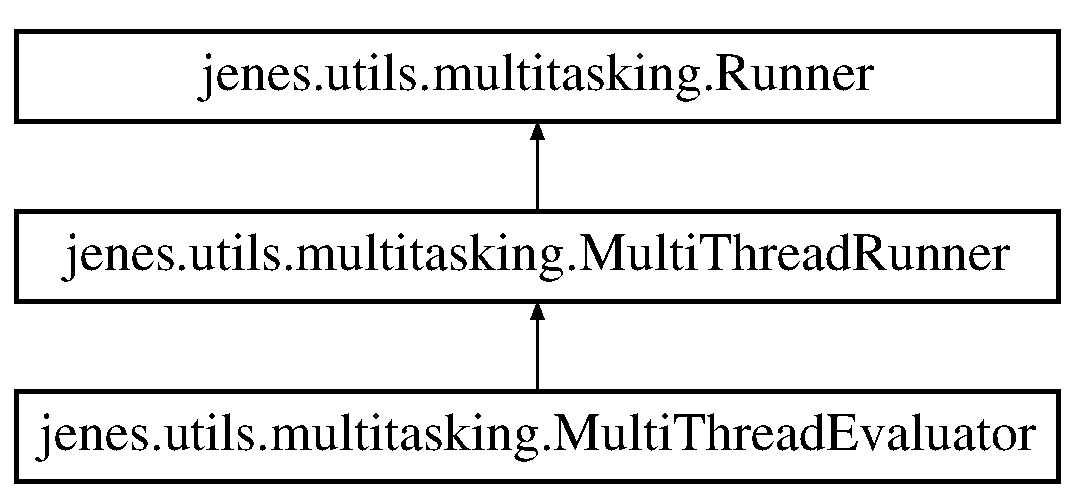
\includegraphics[height=3cm]{classjenes_1_1utils_1_1multitasking_1_1_multi_thread_evaluator}
\end{center}
\end{figure}
\subsection*{Public Member Functions}
\begin{CompactItemize}
\item 
\hyperlink{classjenes_1_1utils_1_1multitasking_1_1_multi_thread_evaluator_842d648ae03a8d7f835a24c522d229ae}{MultiThreadEvaluator} (int nthreads)
\item 
\hyperlink{classjenes_1_1utils_1_1multitasking_1_1_multi_thread_evaluator_c9949bf8de0efb0cb47feb2df56140ff}{MultiThreadEvaluator} ()
\item 
void \hyperlink{classjenes_1_1utils_1_1multitasking_1_1_multi_thread_evaluator_2a9d9427ca8c2b8a9dfc541c85bada42}{onEvaluationBegin} (Population pop, boolean forced)
\item 
synchronized void \hyperlink{classjenes_1_1utils_1_1multitasking_1_1_multi_thread_evaluator_d99c13b137f1089a9f30377548b42e25}{evaluateIndividual} (Individual individual)
\item 
synchronized void \hyperlink{classjenes_1_1utils_1_1multitasking_1_1_multi_thread_evaluator_3cd56b43989da43e4b3c2b79260d5f5f}{onEvaluationEnd} ()
\end{CompactItemize}
\subsection*{Classes}
\begin{CompactItemize}
\item 
class \textbf{EvaluationTask}
\end{CompactItemize}


\subsection{Detailed Description}
This class represent a simple implementation of a multi thread runner

\begin{Desc}
\item[Since:]2.0\end{Desc}
\begin{Desc}
\item[See also:]\hyperlink{classjenes_1_1utils_1_1multitasking_1_1_multi_thread_runner}{MultiThreadRunner} \end{Desc}


\subsection{Constructor \& Destructor Documentation}
\hypertarget{classjenes_1_1utils_1_1multitasking_1_1_multi_thread_evaluator_842d648ae03a8d7f835a24c522d229ae}{
\index{jenes::utils::multitasking::MultiThreadEvaluator@{jenes::utils::multitasking::MultiThreadEvaluator}!MultiThreadEvaluator@{MultiThreadEvaluator}}
\index{MultiThreadEvaluator@{MultiThreadEvaluator}!jenes::utils::multitasking::MultiThreadEvaluator@{jenes::utils::multitasking::MultiThreadEvaluator}}
\subsubsection[MultiThreadEvaluator]{\setlength{\rightskip}{0pt plus 5cm}jenes.utils.multitasking.MultiThreadEvaluator.MultiThreadEvaluator (int {\em nthreads})}}
\label{classjenes_1_1utils_1_1multitasking_1_1_multi_thread_evaluator_842d648ae03a8d7f835a24c522d229ae}


Default constructor that define the thread number to use \begin{Desc}
\item[Parameters:]
\begin{description}
\item[{\em nthreads}]\end{description}
\end{Desc}
\begin{Desc}
\item[See also:]\hyperlink{classjenes_1_1utils_1_1multitasking_1_1_multi_thread_runner_6319362b08c06d8bf26989407d223c31}{MultiThreadRunner.MultiThreadRunner(int)} \end{Desc}
\hypertarget{classjenes_1_1utils_1_1multitasking_1_1_multi_thread_evaluator_c9949bf8de0efb0cb47feb2df56140ff}{
\index{jenes::utils::multitasking::MultiThreadEvaluator@{jenes::utils::multitasking::MultiThreadEvaluator}!MultiThreadEvaluator@{MultiThreadEvaluator}}
\index{MultiThreadEvaluator@{MultiThreadEvaluator}!jenes::utils::multitasking::MultiThreadEvaluator@{jenes::utils::multitasking::MultiThreadEvaluator}}
\subsubsection[MultiThreadEvaluator]{\setlength{\rightskip}{0pt plus 5cm}jenes.utils.multitasking.MultiThreadEvaluator.MultiThreadEvaluator ()}}
\label{classjenes_1_1utils_1_1multitasking_1_1_multi_thread_evaluator_c9949bf8de0efb0cb47feb2df56140ff}


Default constructor that generates an execution enviroinment with a number of threads equals to the number of phisical cores. \begin{Desc}
\item[See also:]\hyperlink{classjenes_1_1utils_1_1multitasking_1_1_multi_thread_runner_b0815486f3159f086cd06ccab94df319}{MultiThreadRunner.MultiThreadRunner()} \end{Desc}


\subsection{Member Function Documentation}
\hypertarget{classjenes_1_1utils_1_1multitasking_1_1_multi_thread_evaluator_2a9d9427ca8c2b8a9dfc541c85bada42}{
\index{jenes::utils::multitasking::MultiThreadEvaluator@{jenes::utils::multitasking::MultiThreadEvaluator}!onEvaluationBegin@{onEvaluationBegin}}
\index{onEvaluationBegin@{onEvaluationBegin}!jenes::utils::multitasking::MultiThreadEvaluator@{jenes::utils::multitasking::MultiThreadEvaluator}}
\subsubsection[onEvaluationBegin]{\setlength{\rightskip}{0pt plus 5cm}void jenes.utils.multitasking.MultiThreadEvaluator.onEvaluationBegin (Population {\em pop}, \/  boolean {\em forced})}}
\label{classjenes_1_1utils_1_1multitasking_1_1_multi_thread_evaluator_2a9d9427ca8c2b8a9dfc541c85bada42}


Call-back invoked soon before the \hyperlink{}{Population} evaluation starts using the default \hyperlink{}{Fitness} defined per \hyperlink{}{GeneticAlgorithm}

\begin{Desc}
\item[Parameters:]
\begin{description}
\item[{\em pop}]the population that will be evaluated \item[{\em forced}]if each individual of the population will be forced to be evaluated \end{description}
\end{Desc}


Reimplemented from \hyperlink{classjenes_1_1utils_1_1multitasking_1_1_runner_6ec13cf0fb2ff03461a3a397421505cf}{jenes.utils.multitasking.Runner}.\hypertarget{classjenes_1_1utils_1_1multitasking_1_1_multi_thread_evaluator_d99c13b137f1089a9f30377548b42e25}{
\index{jenes::utils::multitasking::MultiThreadEvaluator@{jenes::utils::multitasking::MultiThreadEvaluator}!evaluateIndividual@{evaluateIndividual}}
\index{evaluateIndividual@{evaluateIndividual}!jenes::utils::multitasking::MultiThreadEvaluator@{jenes::utils::multitasking::MultiThreadEvaluator}}
\subsubsection[evaluateIndividual]{\setlength{\rightskip}{0pt plus 5cm}synchronized void jenes.utils.multitasking.MultiThreadEvaluator.evaluateIndividual (Individual {\em individual})\hspace{0.3cm}{\tt  \mbox{[}virtual\mbox{]}}}}
\label{classjenes_1_1utils_1_1multitasking_1_1_multi_thread_evaluator_d99c13b137f1089a9f30377548b42e25}


Call-back invoked in substitution to \hyperlink{}{GeneticAlgorithm\#evaluateIndividual(jenes.population.Individual)} \begin{Desc}
\item[Parameters:]
\begin{description}
\item[{\em individual}]\end{description}
\end{Desc}


Implements \hyperlink{classjenes_1_1utils_1_1multitasking_1_1_runner_250c5e0ffdb86ef0bb0e78e625a449e7}{jenes.utils.multitasking.Runner}.\hypertarget{classjenes_1_1utils_1_1multitasking_1_1_multi_thread_evaluator_3cd56b43989da43e4b3c2b79260d5f5f}{
\index{jenes::utils::multitasking::MultiThreadEvaluator@{jenes::utils::multitasking::MultiThreadEvaluator}!onEvaluationEnd@{onEvaluationEnd}}
\index{onEvaluationEnd@{onEvaluationEnd}!jenes::utils::multitasking::MultiThreadEvaluator@{jenes::utils::multitasking::MultiThreadEvaluator}}
\subsubsection[onEvaluationEnd]{\setlength{\rightskip}{0pt plus 5cm}synchronized void jenes.utils.multitasking.MultiThreadEvaluator.onEvaluationEnd ()}}
\label{classjenes_1_1utils_1_1multitasking_1_1_multi_thread_evaluator_3cd56b43989da43e4b3c2b79260d5f5f}


Call-back invoked soon after the evaluation phase has been performed. \par
 WARNING: the method is called before the elapsed time per evaluation is computed so a huge work could affect measurements. 

Reimplemented from \hyperlink{classjenes_1_1utils_1_1multitasking_1_1_runner_82c84ad942296d62849248b107ec3a2c}{jenes.utils.multitasking.Runner}.

The documentation for this class was generated from the following file:\begin{CompactItemize}
\item 
src/jenes/utils/multitasking/MultiThreadEvaluator.java\end{CompactItemize}

\hypertarget{classjenes_1_1tutorials_1_1problem11_1_1_multi_thread_example}{
\section{jenes.tutorials.problem11.MultiThreadExample Class Reference}
\label{classjenes_1_1tutorials_1_1problem11_1_1_multi_thread_example}\index{jenes::tutorials::problem11::MultiThreadExample@{jenes::tutorials::problem11::MultiThreadExample}}
}
\subsection*{Static Public Member Functions}
\begin{CompactItemize}
\item 
static void \hyperlink{classjenes_1_1tutorials_1_1problem11_1_1_multi_thread_example_78352360229430486f32eb26551cb118}{main} (String...a)  throws Exception
\end{CompactItemize}


\subsection{Detailed Description}
This class represent a simple example of how to use multi-thread feature in Jenes 2.0

\begin{Desc}
\item[Since:]2.0 \end{Desc}


\subsection{Member Function Documentation}
\hypertarget{classjenes_1_1tutorials_1_1problem11_1_1_multi_thread_example_78352360229430486f32eb26551cb118}{
\index{jenes::tutorials::problem11::MultiThreadExample@{jenes::tutorials::problem11::MultiThreadExample}!main@{main}}
\index{main@{main}!jenes::tutorials::problem11::MultiThreadExample@{jenes::tutorials::problem11::MultiThreadExample}}
\subsubsection[main]{\setlength{\rightskip}{0pt plus 5cm}static void jenes.tutorials.problem11.MultiThreadExample.main (String... {\em a})  throws Exception\hspace{0.3cm}{\tt  \mbox{[}static\mbox{]}}}}
\label{classjenes_1_1tutorials_1_1problem11_1_1_multi_thread_example_78352360229430486f32eb26551cb118}




The angle to use as target for matching 

The documentation for this class was generated from the following file:\begin{CompactItemize}
\item 
src/jenes/tutorials/problem11/MultiThreadExample.java\end{CompactItemize}

\hypertarget{classjenes_1_1utils_1_1multitasking_1_1_multi_thread_runner}{
\section{jenes.utils.multitasking.MultiThreadRunner Class Reference}
\label{classjenes_1_1utils_1_1multitasking_1_1_multi_thread_runner}\index{jenes::utils::multitasking::MultiThreadRunner@{jenes::utils::multitasking::MultiThreadRunner}}
}
Inheritance diagram for jenes.utils.multitasking.MultiThreadRunner::\begin{figure}[H]
\begin{center}
\leavevmode
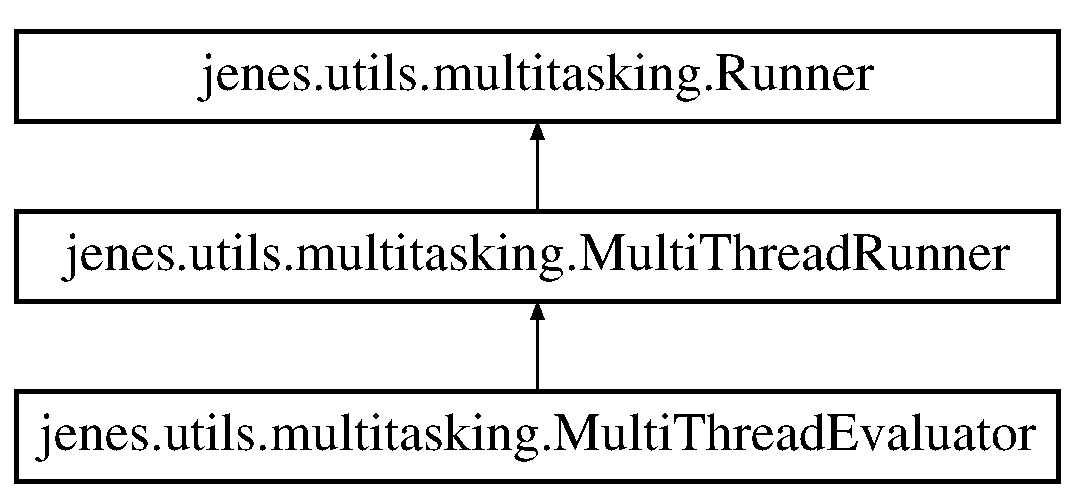
\includegraphics[height=3cm]{classjenes_1_1utils_1_1multitasking_1_1_multi_thread_runner}
\end{center}
\end{figure}
\subsection*{Public Member Functions}
\begin{CompactItemize}
\item 
\hyperlink{classjenes_1_1utils_1_1multitasking_1_1_multi_thread_runner_b0815486f3159f086cd06ccab94df319}{MultiThreadRunner} ()
\item 
\hyperlink{classjenes_1_1utils_1_1multitasking_1_1_multi_thread_runner_6319362b08c06d8bf26989407d223c31}{MultiThreadRunner} (int nthreads)
\item 
int \hyperlink{classjenes_1_1utils_1_1multitasking_1_1_multi_thread_runner_69370630a898026070fe8e806cec8fe0}{getNthreads} ()
\item 
void \hyperlink{classjenes_1_1utils_1_1multitasking_1_1_multi_thread_runner_52fc59a28c3187e84b871b9b823b7f43}{start} (boolean reset)
\item 
void \hyperlink{classjenes_1_1utils_1_1multitasking_1_1_multi_thread_runner_5f00a9b63ff1322d586ad62ec060d597}{stop} ()
\end{CompactItemize}
\subsection*{Protected Attributes}
\begin{CompactItemize}
\item 
\hypertarget{classjenes_1_1utils_1_1multitasking_1_1_multi_thread_runner_a20fe700a6b2abd3694b4a1d5629db8f}{
int \textbf{nthreads}}
\label{classjenes_1_1utils_1_1multitasking_1_1_multi_thread_runner_a20fe700a6b2abd3694b4a1d5629db8f}

\item 
ExecutorService \hyperlink{classjenes_1_1utils_1_1multitasking_1_1_multi_thread_runner_fd9939cc7a261bd4bb6c8f3de6f58337}{threadGroup}
\end{CompactItemize}


\subsection{Detailed Description}
This class provide the basic implementation of a multi-thread enviroinment for \hyperlink{}{GeneticAlgorithm}

\begin{Desc}
\item[Since:]2.0 \end{Desc}


\subsection{Constructor \& Destructor Documentation}
\hypertarget{classjenes_1_1utils_1_1multitasking_1_1_multi_thread_runner_b0815486f3159f086cd06ccab94df319}{
\index{jenes::utils::multitasking::MultiThreadRunner@{jenes::utils::multitasking::MultiThreadRunner}!MultiThreadRunner@{MultiThreadRunner}}
\index{MultiThreadRunner@{MultiThreadRunner}!jenes::utils::multitasking::MultiThreadRunner@{jenes::utils::multitasking::MultiThreadRunner}}
\subsubsection[MultiThreadRunner]{\setlength{\rightskip}{0pt plus 5cm}jenes.utils.multitasking.MultiThreadRunner.MultiThreadRunner ()}}
\label{classjenes_1_1utils_1_1multitasking_1_1_multi_thread_runner_b0815486f3159f086cd06ccab94df319}


Default constructor. This will instantiate a \hyperlink{classjenes_1_1utils_1_1multitasking_1_1_multi_thread_runner}{MultiThreadRunner} envoiroinment wich thread number is equals to the maximum number of processor phisical avaible to the host Java Virtual Machine. \par
 This approach minimize the overhead in managing the thread because the latest JVMs could try to dispach each thread on a different phisical processor obtaining the best speed-up in performances. \begin{Desc}
\item[See also:]\hyperlink{classjenes_1_1utils_1_1multitasking_1_1_multi_thread_runner_6319362b08c06d8bf26989407d223c31}{MultiThreadRunner(int)} 

Runtime.availableProcessors() \end{Desc}
\hypertarget{classjenes_1_1utils_1_1multitasking_1_1_multi_thread_runner_6319362b08c06d8bf26989407d223c31}{
\index{jenes::utils::multitasking::MultiThreadRunner@{jenes::utils::multitasking::MultiThreadRunner}!MultiThreadRunner@{MultiThreadRunner}}
\index{MultiThreadRunner@{MultiThreadRunner}!jenes::utils::multitasking::MultiThreadRunner@{jenes::utils::multitasking::MultiThreadRunner}}
\subsubsection[MultiThreadRunner]{\setlength{\rightskip}{0pt plus 5cm}jenes.utils.multitasking.MultiThreadRunner.MultiThreadRunner (int {\em nthreads})}}
\label{classjenes_1_1utils_1_1multitasking_1_1_multi_thread_runner_6319362b08c06d8bf26989407d223c31}


This will instantiate a \hyperlink{classjenes_1_1utils_1_1multitasking_1_1_multi_thread_runner}{MultiThreadRunner} enviroinment with a fixed thread pool sized as defined by argument \begin{Desc}
\item[Parameters:]
\begin{description}
\item[{\em nthreads}]the number of threads to use to parallelize algorithm execution \end{description}
\end{Desc}


\subsection{Member Function Documentation}
\hypertarget{classjenes_1_1utils_1_1multitasking_1_1_multi_thread_runner_69370630a898026070fe8e806cec8fe0}{
\index{jenes::utils::multitasking::MultiThreadRunner@{jenes::utils::multitasking::MultiThreadRunner}!getNthreads@{getNthreads}}
\index{getNthreads@{getNthreads}!jenes::utils::multitasking::MultiThreadRunner@{jenes::utils::multitasking::MultiThreadRunner}}
\subsubsection[getNthreads]{\setlength{\rightskip}{0pt plus 5cm}int jenes.utils.multitasking.MultiThreadRunner.getNthreads ()}}
\label{classjenes_1_1utils_1_1multitasking_1_1_multi_thread_runner_69370630a898026070fe8e806cec8fe0}


Get the number of threads currently setted for this enviroinment \begin{Desc}
\item[Returns:]\end{Desc}
\hypertarget{classjenes_1_1utils_1_1multitasking_1_1_multi_thread_runner_52fc59a28c3187e84b871b9b823b7f43}{
\index{jenes::utils::multitasking::MultiThreadRunner@{jenes::utils::multitasking::MultiThreadRunner}!start@{start}}
\index{start@{start}!jenes::utils::multitasking::MultiThreadRunner@{jenes::utils::multitasking::MultiThreadRunner}}
\subsubsection[start]{\setlength{\rightskip}{0pt plus 5cm}void jenes.utils.multitasking.MultiThreadRunner.start (boolean {\em reset})}}
\label{classjenes_1_1utils_1_1multitasking_1_1_multi_thread_runner_52fc59a28c3187e84b871b9b823b7f43}


Call-back invoked by \hyperlink{}{GeneticAlgorithm\#start(boolean)} \begin{Desc}
\item[Parameters:]
\begin{description}
\item[{\em reset}]\end{description}
\end{Desc}


Reimplemented from \hyperlink{classjenes_1_1utils_1_1multitasking_1_1_runner_5dc1ed49495150ff26ec5194010b00e4}{jenes.utils.multitasking.Runner}.\hypertarget{classjenes_1_1utils_1_1multitasking_1_1_multi_thread_runner_5f00a9b63ff1322d586ad62ec060d597}{
\index{jenes::utils::multitasking::MultiThreadRunner@{jenes::utils::multitasking::MultiThreadRunner}!stop@{stop}}
\index{stop@{stop}!jenes::utils::multitasking::MultiThreadRunner@{jenes::utils::multitasking::MultiThreadRunner}}
\subsubsection[stop]{\setlength{\rightskip}{0pt plus 5cm}void jenes.utils.multitasking.MultiThreadRunner.stop ()}}
\label{classjenes_1_1utils_1_1multitasking_1_1_multi_thread_runner_5f00a9b63ff1322d586ad62ec060d597}


Call-back called soon after \hyperlink{}{GeneticAlgorithm\#onStop(long)} 

Reimplemented from \hyperlink{classjenes_1_1utils_1_1multitasking_1_1_runner_c89e8ac54daba2e326e687662ff9f7b0}{jenes.utils.multitasking.Runner}.

\subsection{Member Data Documentation}
\hypertarget{classjenes_1_1utils_1_1multitasking_1_1_multi_thread_runner_fd9939cc7a261bd4bb6c8f3de6f58337}{
\index{jenes::utils::multitasking::MultiThreadRunner@{jenes::utils::multitasking::MultiThreadRunner}!threadGroup@{threadGroup}}
\index{threadGroup@{threadGroup}!jenes::utils::multitasking::MultiThreadRunner@{jenes::utils::multitasking::MultiThreadRunner}}
\subsubsection[threadGroup]{\setlength{\rightskip}{0pt plus 5cm}ExecutorService {\bf jenes.utils.multitasking.MultiThreadRunner.threadGroup}\hspace{0.3cm}{\tt  \mbox{[}protected\mbox{]}}}}
\label{classjenes_1_1utils_1_1multitasking_1_1_multi_thread_runner_fd9939cc7a261bd4bb6c8f3de6f58337}


Instance of the thread pool 

The documentation for this class was generated from the following file:\begin{CompactItemize}
\item 
src/jenes/utils/multitasking/MultiThreadRunner.java\end{CompactItemize}

\hypertarget{classjenes_1_1stage_1_1operator_1_1_mutator_3_01_t_01extends_01_chromosome_01_4}{
\section{jenes.stage.operator.Mutator$<$ T extends Chromosome $>$ Class Reference}
\label{classjenes_1_1stage_1_1operator_1_1_mutator_3_01_t_01extends_01_chromosome_01_4}\index{jenes::stage::operator::Mutator$<$ T extends Chromosome $>$@{jenes::stage::operator::Mutator$<$ T extends Chromosome $>$}}
}
\subsection*{Public Member Functions}
\begin{CompactItemize}
\item 
\hyperlink{classjenes_1_1stage_1_1operator_1_1_mutator_3_01_t_01extends_01_chromosome_01_4_01aea5c94d65f99cca8a24be7250a06a}{Mutator} (double \hyperlink{classjenes_1_1stage_1_1operator_1_1_mutator_3_01_t_01extends_01_chromosome_01_4_60f38eb7afd1ad6a7d1c0c639df2d5fe}{probability})
\item 
double \hyperlink{classjenes_1_1stage_1_1operator_1_1_mutator_3_01_t_01extends_01_chromosome_01_4_f8cd41f87d99e8bc5d00bf9a21ffcd86}{getProbability} ()
\item 
void \hyperlink{classjenes_1_1stage_1_1operator_1_1_mutator_3_01_t_01extends_01_chromosome_01_4_49b8a34032a575badd2080d6c90397cb}{setProbability} (double \hyperlink{classjenes_1_1stage_1_1operator_1_1_mutator_3_01_t_01extends_01_chromosome_01_4_60f38eb7afd1ad6a7d1c0c639df2d5fe}{probability})
\item 
\hypertarget{classjenes_1_1stage_1_1operator_1_1_mutator_3_01_t_01extends_01_chromosome_01_4_091269db32219198b26860ee4b295345}{
final void \textbf{process} (Population$<$ T $>$ in, Population$<$ T $>$ out)  throws StageException }
\label{classjenes_1_1stage_1_1operator_1_1_mutator_3_01_t_01extends_01_chromosome_01_4_091269db32219198b26860ee4b295345}

\end{CompactItemize}
\subsection*{Protected Member Functions}
\begin{CompactItemize}
\item 
abstract void \hyperlink{classjenes_1_1stage_1_1operator_1_1_mutator_3_01_t_01extends_01_chromosome_01_4_5ea1c6fd8d4ed580d70e1fafd85bb3a8}{mutate} (Individual$<$ T $>$ t)
\end{CompactItemize}
\subsection*{Protected Attributes}
\begin{CompactItemize}
\item 
double \hyperlink{classjenes_1_1stage_1_1operator_1_1_mutator_3_01_t_01extends_01_chromosome_01_4_60f38eb7afd1ad6a7d1c0c639df2d5fe}{probability}
\end{CompactItemize}
\subsection*{Classes}
\begin{CompactItemize}
\item 
class \hyperlink{classjenes_1_1stage_1_1operator_1_1_mutator_3_01_t_01extends_01_chromosome_01_4_1_1_statistics}{Statistics}
\end{CompactItemize}


\subsection{Detailed Description}
A generic mutation operator. The operation is executed according to a mutation probability. 

The actual operator is implemented by subclassing this abstract class and providing the \hyperlink{}{Mutator\#mutate(Individual)} implementation: the method is required to mutate an \hyperlink{}{Individual} according to a mutation strategy. No new individual copies have to be created during the mutation operation: the individual specified at the \hyperlink{}{Mutator\#mutate(Individual)} will take parte to the output mutator population. 

A \hyperlink{}{Mutator.Statistics} is associated to each mutator operator.

\begin{Desc}
\item[Parameters:]
\begin{description}
\item[{\em $<$T$>$}]The class of chromosomes to work with.\end{description}
\end{Desc}
\begin{Desc}
\item[Version:]1.2 \end{Desc}
\begin{Desc}
\item[Since:]1.0\end{Desc}
\begin{Desc}
\item[See also:]Individual 

Population \end{Desc}


\subsection{Constructor \& Destructor Documentation}
\hypertarget{classjenes_1_1stage_1_1operator_1_1_mutator_3_01_t_01extends_01_chromosome_01_4_01aea5c94d65f99cca8a24be7250a06a}{
\index{jenes::stage::operator::Mutator$<$ T extends Chromosome $>$@{jenes::stage::operator::Mutator$<$ T extends Chromosome $>$}!Mutator@{Mutator}}
\index{Mutator@{Mutator}!jenes::stage::operator::Mutator< T extends Chromosome >@{jenes::stage::operator::Mutator$<$ T extends Chromosome $>$}}
\subsubsection[Mutator]{\setlength{\rightskip}{0pt plus 5cm}jenes.stage.operator.Mutator$<$ T extends Chromosome $>$.Mutator (double {\em probability})}}
\label{classjenes_1_1stage_1_1operator_1_1_mutator_3_01_t_01extends_01_chromosome_01_4_01aea5c94d65f99cca8a24be7250a06a}


Constructs a new mutator instance with the specified mutator probability

\begin{Desc}
\item[Parameters:]
\begin{description}
\item[{\em probability}]the mutator probability \end{description}
\end{Desc}


\subsection{Member Function Documentation}
\hypertarget{classjenes_1_1stage_1_1operator_1_1_mutator_3_01_t_01extends_01_chromosome_01_4_f8cd41f87d99e8bc5d00bf9a21ffcd86}{
\index{jenes::stage::operator::Mutator$<$ T extends Chromosome $>$@{jenes::stage::operator::Mutator$<$ T extends Chromosome $>$}!getProbability@{getProbability}}
\index{getProbability@{getProbability}!jenes::stage::operator::Mutator< T extends Chromosome >@{jenes::stage::operator::Mutator$<$ T extends Chromosome $>$}}
\subsubsection[getProbability]{\setlength{\rightskip}{0pt plus 5cm}double jenes.stage.operator.Mutator$<$ T extends Chromosome $>$.getProbability ()}}
\label{classjenes_1_1stage_1_1operator_1_1_mutator_3_01_t_01extends_01_chromosome_01_4_f8cd41f87d99e8bc5d00bf9a21ffcd86}


Returns the mutator probability

\begin{Desc}
\item[Returns:]the mutator probability \end{Desc}
\hypertarget{classjenes_1_1stage_1_1operator_1_1_mutator_3_01_t_01extends_01_chromosome_01_4_49b8a34032a575badd2080d6c90397cb}{
\index{jenes::stage::operator::Mutator$<$ T extends Chromosome $>$@{jenes::stage::operator::Mutator$<$ T extends Chromosome $>$}!setProbability@{setProbability}}
\index{setProbability@{setProbability}!jenes::stage::operator::Mutator< T extends Chromosome >@{jenes::stage::operator::Mutator$<$ T extends Chromosome $>$}}
\subsubsection[setProbability]{\setlength{\rightskip}{0pt plus 5cm}void jenes.stage.operator.Mutator$<$ T extends Chromosome $>$.setProbability (double {\em probability})}}
\label{classjenes_1_1stage_1_1operator_1_1_mutator_3_01_t_01extends_01_chromosome_01_4_49b8a34032a575badd2080d6c90397cb}


Sets the mutator probability

\begin{Desc}
\item[Parameters:]
\begin{description}
\item[{\em probability}]the new mutator probability \end{description}
\end{Desc}
\hypertarget{classjenes_1_1stage_1_1operator_1_1_mutator_3_01_t_01extends_01_chromosome_01_4_5ea1c6fd8d4ed580d70e1fafd85bb3a8}{
\index{jenes::stage::operator::Mutator$<$ T extends Chromosome $>$@{jenes::stage::operator::Mutator$<$ T extends Chromosome $>$}!mutate@{mutate}}
\index{mutate@{mutate}!jenes::stage::operator::Mutator< T extends Chromosome >@{jenes::stage::operator::Mutator$<$ T extends Chromosome $>$}}
\subsubsection[mutate]{\setlength{\rightskip}{0pt plus 5cm}abstract void jenes.stage.operator.Mutator$<$ T extends Chromosome $>$.mutate (Individual$<$ T $>$ {\em t})\hspace{0.3cm}{\tt  \mbox{[}protected, pure virtual\mbox{]}}}}
\label{classjenes_1_1stage_1_1operator_1_1_mutator_3_01_t_01extends_01_chromosome_01_4_5ea1c6fd8d4ed580d70e1fafd85bb3a8}


Mutates a single individual. This abstract method is implemented according to a mutation policy

\begin{Desc}
\item[Parameters:]
\begin{description}
\item[{\em t}]the individual to mutate \end{description}
\end{Desc}


\subsection{Member Data Documentation}
\hypertarget{classjenes_1_1stage_1_1operator_1_1_mutator_3_01_t_01extends_01_chromosome_01_4_60f38eb7afd1ad6a7d1c0c639df2d5fe}{
\index{jenes::stage::operator::Mutator$<$ T extends Chromosome $>$@{jenes::stage::operator::Mutator$<$ T extends Chromosome $>$}!probability@{probability}}
\index{probability@{probability}!jenes::stage::operator::Mutator< T extends Chromosome >@{jenes::stage::operator::Mutator$<$ T extends Chromosome $>$}}
\subsubsection[probability]{\setlength{\rightskip}{0pt plus 5cm}double jenes.stage.operator.Mutator$<$ T extends Chromosome $>$.{\bf probability}\hspace{0.3cm}{\tt  \mbox{[}protected\mbox{]}}}}
\label{classjenes_1_1stage_1_1operator_1_1_mutator_3_01_t_01extends_01_chromosome_01_4_60f38eb7afd1ad6a7d1c0c639df2d5fe}


The mutation probablility 

The documentation for this class was generated from the following file:\begin{CompactItemize}
\item 
src/jenes/stage/operator/Mutator.java\end{CompactItemize}

\hypertarget{classjenes_1_1stage_1_1operator_1_1_mutator_3_01_t_01extends_01_chromosome_01_4_1_1_statistics}{
\section{jenes.stage.operator.Mutator$<$ T extends Chromosome $>$.Statistics Class Reference}
\label{classjenes_1_1stage_1_1operator_1_1_mutator_3_01_t_01extends_01_chromosome_01_4_1_1_statistics}\index{jenes::stage::operator::Mutator$<$ T extends Chromosome $>$::Statistics@{jenes::stage::operator::Mutator$<$ T extends Chromosome $>$::Statistics}}
}
\subsection*{Public Member Functions}
\begin{CompactItemize}
\item 
long \hyperlink{classjenes_1_1stage_1_1operator_1_1_mutator_3_01_t_01extends_01_chromosome_01_4_1_1_statistics_fc74de8d8cf1b0d1cdaf9ec3a170c80e}{getMutations} ()
\end{CompactItemize}
\subsection*{Protected Member Functions}
\begin{CompactItemize}
\item 
\hypertarget{classjenes_1_1stage_1_1operator_1_1_mutator_3_01_t_01extends_01_chromosome_01_4_1_1_statistics_f114cf6ccf66e1bd5d5d7337b4e15e28}{
void \textbf{fill} (Operator$<$ T $>$.Statistics stats)}
\label{classjenes_1_1stage_1_1operator_1_1_mutator_3_01_t_01extends_01_chromosome_01_4_1_1_statistics_f114cf6ccf66e1bd5d5d7337b4e15e28}

\end{CompactItemize}
\subsection*{Protected Attributes}
\begin{CompactItemize}
\item 
long \hyperlink{classjenes_1_1stage_1_1operator_1_1_mutator_3_01_t_01extends_01_chromosome_01_4_1_1_statistics_4328be89d9643f783f5c08164a0aa916}{mutations}
\end{CompactItemize}


\subsection{Detailed Description}
A statistics object holding the number of mutation performed and the time spent to execute them. The statistics is available by two methods: \hyperlink{}{Mutator\#getStatistics()} to have a new statistics setted according to the mutator state or \hyperlink{}{Mutator\#updateStatistics(jenes.stage.operator.Operator.Statistics)} to modify an existing statistics according to the mutator state. 

Esamples of use are showed below. 

$<$blockquote$>$\small\begin{alltt}
 Mutator.Statistics stat = a\_mutator.getStatistics();
 \end{alltt}
\normalsize 
$<$/blockquote$>$ 

returns a new statistics object setted according to the specified mutator state. 

$<$blockquote$>$\small\begin{alltt}
 Mutator.Statistics stat = new Mutator.Statistics();
 a\_mutator.updateStatistics(stat);
 \end{alltt}
\normalsize 
$<$/blockquote$>$ 

modifies the existing statistics according to the specified mutator state. 

\subsection{Member Function Documentation}
\hypertarget{classjenes_1_1stage_1_1operator_1_1_mutator_3_01_t_01extends_01_chromosome_01_4_1_1_statistics_fc74de8d8cf1b0d1cdaf9ec3a170c80e}{
\index{jenes::stage::operator::Mutator$<$ T extends Chromosome $>$::Statistics@{jenes::stage::operator::Mutator$<$ T extends Chromosome $>$::Statistics}!getMutations@{getMutations}}
\index{getMutations@{getMutations}!jenes::stage::operator::Mutator< T extends Chromosome >::Statistics@{jenes::stage::operator::Mutator$<$ T extends Chromosome $>$::Statistics}}
\subsubsection[getMutations]{\setlength{\rightskip}{0pt plus 5cm}long jenes.stage.operator.Mutator$<$ T extends Chromosome $>$.Statistics.getMutations ()}}
\label{classjenes_1_1stage_1_1operator_1_1_mutator_3_01_t_01extends_01_chromosome_01_4_1_1_statistics_fc74de8d8cf1b0d1cdaf9ec3a170c80e}


Returns the number of mutations performed

\begin{Desc}
\item[Returns:]the number of mutations performed \end{Desc}


\subsection{Member Data Documentation}
\hypertarget{classjenes_1_1stage_1_1operator_1_1_mutator_3_01_t_01extends_01_chromosome_01_4_1_1_statistics_4328be89d9643f783f5c08164a0aa916}{
\index{jenes::stage::operator::Mutator$<$ T extends Chromosome $>$::Statistics@{jenes::stage::operator::Mutator$<$ T extends Chromosome $>$::Statistics}!mutations@{mutations}}
\index{mutations@{mutations}!jenes::stage::operator::Mutator< T extends Chromosome >::Statistics@{jenes::stage::operator::Mutator$<$ T extends Chromosome $>$::Statistics}}
\subsubsection[mutations]{\setlength{\rightskip}{0pt plus 5cm}long jenes.stage.operator.Mutator$<$ T extends Chromosome $>$.Statistics.mutations\hspace{0.3cm}{\tt  \mbox{[}protected\mbox{]}}}}
\label{classjenes_1_1stage_1_1operator_1_1_mutator_3_01_t_01extends_01_chromosome_01_4_1_1_statistics_4328be89d9643f783f5c08164a0aa916}


Number of mutations performed. 

The documentation for this class was generated from the following file:\begin{CompactItemize}
\item 
src/jenes/stage/operator/Mutator.java\end{CompactItemize}

\hypertarget{classjenes_1_1algorithms_1_1_n_s_g_a2_3_01_t_01extends_01_chromosome_01_4}{
\section{jenes.algorithms.NSGA2$<$ T extends Chromosome $>$ Class Reference}
\label{classjenes_1_1algorithms_1_1_n_s_g_a2_3_01_t_01extends_01_chromosome_01_4}\index{jenes::algorithms::NSGA2$<$ T extends Chromosome $>$@{jenes::algorithms::NSGA2$<$ T extends Chromosome $>$}}
}
Inherits jenes::algorithms::CrowdingGA$<$ T $>$.

\subsection*{Public Member Functions}
\begin{CompactItemize}
\item 
\hyperlink{classjenes_1_1algorithms_1_1_n_s_g_a2_3_01_t_01extends_01_chromosome_01_4_0e9264bdd3c0f0f73fecdc89038b2898}{NSGA2} (Fitness fitness)
\item 
\hyperlink{classjenes_1_1algorithms_1_1_n_s_g_a2_3_01_t_01extends_01_chromosome_01_4_49f57f66489874c5bf12b3f9c89e6fcc}{NSGA2} (final Fitness fitness, final Population$<$ T $>$ population)
\item 
\hyperlink{classjenes_1_1algorithms_1_1_n_s_g_a2_3_01_t_01extends_01_chromosome_01_4_4da7d36c029be00959ea063643833486}{NSGA2} (final Fitness fitness, final Population$<$ T $>$ population, final int generations)
\item 
\hyperlink{classjenes_1_1algorithms_1_1_n_s_g_a2_3_01_t_01extends_01_chromosome_01_4_c0873ceec23f2908e64650b2e0f2b62a}{NSGA2} (final Fitness fitness, final Population$<$ T $>$ population, final int generations, final int trials)
\end{CompactItemize}
\subsection*{Static Public Attributes}
\begin{CompactItemize}
\item 
static final int \hyperlink{classjenes_1_1algorithms_1_1_n_s_g_a2_3_01_t_01extends_01_chromosome_01_4_63cad03fd3ef9a70933b35dbe043b4ea}{DEFAULT\_\-GENERATION\_\-LIMIT} = 100
\item 
static final int \hyperlink{classjenes_1_1algorithms_1_1_n_s_g_a2_3_01_t_01extends_01_chromosome_01_4_a480c4702a4fbf2bb1ec8c8f9c7dc82b}{DEFAULT\_\-SELECTION\_\-TRIALS} = 3
\end{CompactItemize}
\subsection*{Classes}
\begin{CompactItemize}
\item 
class \textbf{DominanceCrowder$<$ C extends Chromosome $>$}
\end{CompactItemize}


\subsection{Detailed Description}
Multi-objective genetic algorithm as proposed by Deb.

\begin{Desc}
\item[Version:]2.0 \end{Desc}
\begin{Desc}
\item[Since:]2.0 \end{Desc}


\subsection{Constructor \& Destructor Documentation}
\hypertarget{classjenes_1_1algorithms_1_1_n_s_g_a2_3_01_t_01extends_01_chromosome_01_4_0e9264bdd3c0f0f73fecdc89038b2898}{
\index{jenes::algorithms::NSGA2$<$ T extends Chromosome $>$@{jenes::algorithms::NSGA2$<$ T extends Chromosome $>$}!NSGA2@{NSGA2}}
\index{NSGA2@{NSGA2}!jenes::algorithms::NSGA2< T extends Chromosome >@{jenes::algorithms::NSGA2$<$ T extends Chromosome $>$}}
\subsubsection[NSGA2]{\setlength{\rightskip}{0pt plus 5cm}jenes.algorithms.NSGA2$<$ T extends Chromosome $>$.NSGA2 (Fitness {\em fitness})}}
\label{classjenes_1_1algorithms_1_1_n_s_g_a2_3_01_t_01extends_01_chromosome_01_4_0e9264bdd3c0f0f73fecdc89038b2898}


Default constructor \begin{Desc}
\item[Parameters:]
\begin{description}
\item[{\em fitness}]the fitness function to adopt in evolving this algorithm \end{description}
\end{Desc}
\hypertarget{classjenes_1_1algorithms_1_1_n_s_g_a2_3_01_t_01extends_01_chromosome_01_4_49f57f66489874c5bf12b3f9c89e6fcc}{
\index{jenes::algorithms::NSGA2$<$ T extends Chromosome $>$@{jenes::algorithms::NSGA2$<$ T extends Chromosome $>$}!NSGA2@{NSGA2}}
\index{NSGA2@{NSGA2}!jenes::algorithms::NSGA2< T extends Chromosome >@{jenes::algorithms::NSGA2$<$ T extends Chromosome $>$}}
\subsubsection[NSGA2]{\setlength{\rightskip}{0pt plus 5cm}jenes.algorithms.NSGA2$<$ T extends Chromosome $>$.NSGA2 (final Fitness {\em fitness}, \/  final Population$<$ T $>$ {\em population})}}
\label{classjenes_1_1algorithms_1_1_n_s_g_a2_3_01_t_01extends_01_chromosome_01_4_49f57f66489874c5bf12b3f9c89e6fcc}


Generates a new NSGA2 instance 

\begin{Desc}
\item[Parameters:]
\begin{description}
\item[{\em fitness}]the fitness function to adopt in evolving this algorithm \item[{\em population}]the initial population \end{description}
\end{Desc}
\hypertarget{classjenes_1_1algorithms_1_1_n_s_g_a2_3_01_t_01extends_01_chromosome_01_4_4da7d36c029be00959ea063643833486}{
\index{jenes::algorithms::NSGA2$<$ T extends Chromosome $>$@{jenes::algorithms::NSGA2$<$ T extends Chromosome $>$}!NSGA2@{NSGA2}}
\index{NSGA2@{NSGA2}!jenes::algorithms::NSGA2< T extends Chromosome >@{jenes::algorithms::NSGA2$<$ T extends Chromosome $>$}}
\subsubsection[NSGA2]{\setlength{\rightskip}{0pt plus 5cm}jenes.algorithms.NSGA2$<$ T extends Chromosome $>$.NSGA2 (final Fitness {\em fitness}, \/  final Population$<$ T $>$ {\em population}, \/  final int {\em generations})}}
\label{classjenes_1_1algorithms_1_1_n_s_g_a2_3_01_t_01extends_01_chromosome_01_4_4da7d36c029be00959ea063643833486}


Generates a new NSGA2 instance 

\begin{Desc}
\item[Parameters:]
\begin{description}
\item[{\em fitness}]the fitness function to adopt in evolving this algorithm \item[{\em population}]the initial population \item[{\em generations}]the generation limit \end{description}
\end{Desc}
\hypertarget{classjenes_1_1algorithms_1_1_n_s_g_a2_3_01_t_01extends_01_chromosome_01_4_c0873ceec23f2908e64650b2e0f2b62a}{
\index{jenes::algorithms::NSGA2$<$ T extends Chromosome $>$@{jenes::algorithms::NSGA2$<$ T extends Chromosome $>$}!NSGA2@{NSGA2}}
\index{NSGA2@{NSGA2}!jenes::algorithms::NSGA2< T extends Chromosome >@{jenes::algorithms::NSGA2$<$ T extends Chromosome $>$}}
\subsubsection[NSGA2]{\setlength{\rightskip}{0pt plus 5cm}jenes.algorithms.NSGA2$<$ T extends Chromosome $>$.NSGA2 (final Fitness {\em fitness}, \/  final Population$<$ T $>$ {\em population}, \/  final int {\em generations}, \/  final int {\em trials})}}
\label{classjenes_1_1algorithms_1_1_n_s_g_a2_3_01_t_01extends_01_chromosome_01_4_c0873ceec23f2908e64650b2e0f2b62a}


Generates a new NSGA2 instance 

\begin{Desc}
\item[Parameters:]
\begin{description}
\item[{\em fitness}]the fitness function to adopt in evolving this algorithm \item[{\em population}]the initial population \item[{\em generations}]the generation limit \item[{\em trials}]number of attempts in tournament selector \end{description}
\end{Desc}
\begin{Desc}
\item[See also:]TournamentSelector \end{Desc}


\subsection{Member Data Documentation}
\hypertarget{classjenes_1_1algorithms_1_1_n_s_g_a2_3_01_t_01extends_01_chromosome_01_4_63cad03fd3ef9a70933b35dbe043b4ea}{
\index{jenes::algorithms::NSGA2$<$ T extends Chromosome $>$@{jenes::algorithms::NSGA2$<$ T extends Chromosome $>$}!DEFAULT\_\-GENERATION\_\-LIMIT@{DEFAULT\_\-GENERATION\_\-LIMIT}}
\index{DEFAULT\_\-GENERATION\_\-LIMIT@{DEFAULT\_\-GENERATION\_\-LIMIT}!jenes::algorithms::NSGA2< T extends Chromosome >@{jenes::algorithms::NSGA2$<$ T extends Chromosome $>$}}
\subsubsection[DEFAULT\_\-GENERATION\_\-LIMIT]{\setlength{\rightskip}{0pt plus 5cm}final int jenes.algorithms.NSGA2$<$ T extends Chromosome $>$.{\bf DEFAULT\_\-GENERATION\_\-LIMIT} = 100\hspace{0.3cm}{\tt  \mbox{[}static\mbox{]}}}}
\label{classjenes_1_1algorithms_1_1_n_s_g_a2_3_01_t_01extends_01_chromosome_01_4_63cad03fd3ef9a70933b35dbe043b4ea}


The default generation limit \hypertarget{classjenes_1_1algorithms_1_1_n_s_g_a2_3_01_t_01extends_01_chromosome_01_4_a480c4702a4fbf2bb1ec8c8f9c7dc82b}{
\index{jenes::algorithms::NSGA2$<$ T extends Chromosome $>$@{jenes::algorithms::NSGA2$<$ T extends Chromosome $>$}!DEFAULT\_\-SELECTION\_\-TRIALS@{DEFAULT\_\-SELECTION\_\-TRIALS}}
\index{DEFAULT\_\-SELECTION\_\-TRIALS@{DEFAULT\_\-SELECTION\_\-TRIALS}!jenes::algorithms::NSGA2< T extends Chromosome >@{jenes::algorithms::NSGA2$<$ T extends Chromosome $>$}}
\subsubsection[DEFAULT\_\-SELECTION\_\-TRIALS]{\setlength{\rightskip}{0pt plus 5cm}final int jenes.algorithms.NSGA2$<$ T extends Chromosome $>$.{\bf DEFAULT\_\-SELECTION\_\-TRIALS} = 3\hspace{0.3cm}{\tt  \mbox{[}static\mbox{]}}}}
\label{classjenes_1_1algorithms_1_1_n_s_g_a2_3_01_t_01extends_01_chromosome_01_4_a480c4702a4fbf2bb1ec8c8f9c7dc82b}


The default number of attempts to \hyperlink{}{TournamentSelector} 

The documentation for this class was generated from the following file:\begin{CompactItemize}
\item 
src/jenes/algorithms/NSGA2.java\end{CompactItemize}

\hypertarget{classjenes_1_1tutorials_1_1problem8_1_1_numeric_crossover}{
\section{jenes.tutorials.problem8.NumericCrossover Class Reference}
\label{classjenes_1_1tutorials_1_1problem8_1_1_numeric_crossover}\index{jenes::tutorials::problem8::NumericCrossover@{jenes::tutorials::problem8::NumericCrossover}}
}
\subsection*{Static Public Member Functions}
\begin{CompactItemize}
\item 
\hypertarget{classjenes_1_1tutorials_1_1problem8_1_1_numeric_crossover_8af3f285354dc96e81647a03d76d93c5}{
static GeneticAlgorithm$<$ \hyperlink{classjenes_1_1chromosome_1_1_double_chromosome}{DoubleChromosome} $>$ \textbf{buildGA} (Crossover$<$ \hyperlink{classjenes_1_1chromosome_1_1_double_chromosome}{DoubleChromosome} $>$ crossover, int n)}
\label{classjenes_1_1tutorials_1_1problem8_1_1_numeric_crossover_8af3f285354dc96e81647a03d76d93c5}

\item 
\hypertarget{classjenes_1_1tutorials_1_1problem8_1_1_numeric_crossover_ef1de8d283010a790fb20661fae423f2}{
static double \textbf{serror} (Individual ind)}
\label{classjenes_1_1tutorials_1_1problem8_1_1_numeric_crossover_ef1de8d283010a790fb20661fae423f2}

\item 
\hypertarget{classjenes_1_1tutorials_1_1problem8_1_1_numeric_crossover_11da9d09414921591a53cddb601cc203}{
static void \textbf{main} (String...args)}
\label{classjenes_1_1tutorials_1_1problem8_1_1_numeric_crossover_11da9d09414921591a53cddb601cc203}

\end{CompactItemize}
\subsection*{Static Public Attributes}
\begin{CompactItemize}
\item 
\hypertarget{classjenes_1_1tutorials_1_1problem8_1_1_numeric_crossover_f73d636c488b92bf3ae33d19d1f5f5e7}{
static int \textbf{LENGHT} = 3}
\label{classjenes_1_1tutorials_1_1problem8_1_1_numeric_crossover_f73d636c488b92bf3ae33d19d1f5f5e7}

\item 
\hypertarget{classjenes_1_1tutorials_1_1problem8_1_1_numeric_crossover_0a9b3b839ab6677dcbae723434df6551}{
static int \textbf{POPSIZE} = 100}
\label{classjenes_1_1tutorials_1_1problem8_1_1_numeric_crossover_0a9b3b839ab6677dcbae723434df6551}

\item 
\hypertarget{classjenes_1_1tutorials_1_1problem8_1_1_numeric_crossover_5e45487dcf5730d7c628ca85b21160dc}{
static int \textbf{GENLIM} = 300}
\label{classjenes_1_1tutorials_1_1problem8_1_1_numeric_crossover_5e45487dcf5730d7c628ca85b21160dc}

\item 
\hypertarget{classjenes_1_1tutorials_1_1problem8_1_1_numeric_crossover_e4fcf3a595e386c6aeec443dedaba83f}{
static double \textbf{CROSSRATE} = 0.8}
\label{classjenes_1_1tutorials_1_1problem8_1_1_numeric_crossover_e4fcf3a595e386c6aeec443dedaba83f}

\item 
\hypertarget{classjenes_1_1tutorials_1_1problem8_1_1_numeric_crossover_4d0587e4b39b1f74efd20a0c921c38f7}{
static double \textbf{MUTPROB} = 0.02}
\label{classjenes_1_1tutorials_1_1problem8_1_1_numeric_crossover_4d0587e4b39b1f74efd20a0c921c38f7}

\item 
\hypertarget{classjenes_1_1tutorials_1_1problem8_1_1_numeric_crossover_e3c1d4871321a6323d09add505679fe0}{
static double \textbf{RATIO} = 0.6}
\label{classjenes_1_1tutorials_1_1problem8_1_1_numeric_crossover_e3c1d4871321a6323d09add505679fe0}

\end{CompactItemize}


\subsection{Detailed Description}
Tutorial showing how to use IntermediateCrossover and HeursiticCrossover in numerical optimization problems.

\begin{Desc}
\item[Version:]2.0 \end{Desc}
\begin{Desc}
\item[Since:]2.0 \end{Desc}


The documentation for this class was generated from the following file:\begin{CompactItemize}
\item 
src/jenes/tutorials/problem8/NumericCrossover.java\end{CompactItemize}

\hypertarget{classjenes_1_1chromosome_1_1_object_chromosome}{
\section{jenes.chromosome.ObjectChromosome Class Reference}
\label{classjenes_1_1chromosome_1_1_object_chromosome}\index{jenes::chromosome::ObjectChromosome@{jenes::chromosome::ObjectChromosome}}
}
Inherits jenes::chromosome::Chromosome$<$ jenes::chromosome::ObjectChromosome $>$.

\subsection*{Public Member Functions}
\begin{CompactItemize}
\item 
\hyperlink{classjenes_1_1chromosome_1_1_object_chromosome_5af7d34bc1f7260dca1dc5c38135f4a4}{ObjectChromosome} (final AlleleSet set, final int size)
\item 
\hyperlink{classjenes_1_1chromosome_1_1_object_chromosome_59e25d20fb54d53ff2b4adc53177d7d2}{ObjectChromosome} (final \hyperlink{classjenes_1_1chromosome_1_1_object_chromosome}{ObjectChromosome} chromosome)
\item 
\hyperlink{classjenes_1_1chromosome_1_1_object_chromosome_ba090ada4d0f24caaf6f68cfed7800f0}{ObjectChromosome} (final AlleleSet...sets)
\item 
\hyperlink{classjenes_1_1chromosome_1_1_object_chromosome_a6c8dcc77a9129f9634ea02f19d5a968}{ObjectChromosome} (final List$<$ AlleleSet $>$ list)
\item 
\hypertarget{classjenes_1_1chromosome_1_1_object_chromosome_d4b8a3ca38d15a8170b63464149b37aa}{
final void \textbf{setDefaultValueAt} (final int pos)}
\label{classjenes_1_1chromosome_1_1_object_chromosome_d4b8a3ca38d15a8170b63464149b37aa}

\item 
\hypertarget{classjenes_1_1chromosome_1_1_object_chromosome_4aa8eeaac6a20b30c260bfda00c78fe2}{
final \hyperlink{classjenes_1_1chromosome_1_1_object_chromosome}{ObjectChromosome} \textbf{clone} ()}
\label{classjenes_1_1chromosome_1_1_object_chromosome_4aa8eeaac6a20b30c260bfda00c78fe2}

\item 
\hypertarget{classjenes_1_1chromosome_1_1_object_chromosome_26a9d9d7eb049ff88c3321728fd9de07}{
final void \textbf{randomize} ()}
\label{classjenes_1_1chromosome_1_1_object_chromosome_26a9d9d7eb049ff88c3321728fd9de07}

\item 
\hypertarget{classjenes_1_1chromosome_1_1_object_chromosome_ac077d08ae00b9805797d5848a10c1f4}{
final void \textbf{randomize} (final int pos)}
\label{classjenes_1_1chromosome_1_1_object_chromosome_ac077d08ae00b9805797d5848a10c1f4}

\item 
\hypertarget{classjenes_1_1chromosome_1_1_object_chromosome_f85db410fecd769993c248f94396dd53}{
final void \textbf{swap} (final int pos1, final int pos2)}
\label{classjenes_1_1chromosome_1_1_object_chromosome_f85db410fecd769993c248f94396dd53}

\item 
\hypertarget{classjenes_1_1chromosome_1_1_object_chromosome_1e1570b75182f3d244a6d857a6acb7bf}{
final void \textbf{leftShift} (final int from, int to)}
\label{classjenes_1_1chromosome_1_1_object_chromosome_1e1570b75182f3d244a6d857a6acb7bf}

\item 
\hypertarget{classjenes_1_1chromosome_1_1_object_chromosome_584d10eceb2858e0ef88ea7f7c21d83c}{
final void \textbf{rightShift} (final int from, int to)}
\label{classjenes_1_1chromosome_1_1_object_chromosome_584d10eceb2858e0ef88ea7f7c21d83c}

\item 
\hypertarget{classjenes_1_1chromosome_1_1_object_chromosome_12ff61d91455ed5915bcf71c889ea1dd}{
final int \textbf{length} ()}
\label{classjenes_1_1chromosome_1_1_object_chromosome_12ff61d91455ed5915bcf71c889ea1dd}

\item 
\hypertarget{classjenes_1_1chromosome_1_1_object_chromosome_77fd7d633e3663ea8fb63db2857bb1b7}{
final void \textbf{setAs} (final \hyperlink{classjenes_1_1chromosome_1_1_object_chromosome}{ObjectChromosome} chromosome)}
\label{classjenes_1_1chromosome_1_1_object_chromosome_77fd7d633e3663ea8fb63db2857bb1b7}

\item 
\hypertarget{classjenes_1_1chromosome_1_1_object_chromosome_8f0770f15071e71ee86d7ad43541118f}{
final void \textbf{cross} (final \hyperlink{classjenes_1_1chromosome_1_1_object_chromosome}{ObjectChromosome} chromosome, final int from)}
\label{classjenes_1_1chromosome_1_1_object_chromosome_8f0770f15071e71ee86d7ad43541118f}

\item 
\hypertarget{classjenes_1_1chromosome_1_1_object_chromosome_25225ffc89dae70e0b0ddeb21f8f125d}{
final void \textbf{cross} (final \hyperlink{classjenes_1_1chromosome_1_1_object_chromosome}{ObjectChromosome} chromosome, final int from, final int to)}
\label{classjenes_1_1chromosome_1_1_object_chromosome_25225ffc89dae70e0b0ddeb21f8f125d}

\item 
final Object \hyperlink{classjenes_1_1chromosome_1_1_object_chromosome_f221c16bbcd9f03867d2e4295216cc93}{getValue} (final int pos)
\item 
final Object\mbox{[}$\,$\mbox{]} \hyperlink{classjenes_1_1chromosome_1_1_object_chromosome_f41d722cff36fbb837c0038c885de04c}{getValues} ()
\item 
final Object\mbox{[}$\,$\mbox{]} \hyperlink{classjenes_1_1chromosome_1_1_object_chromosome_7476459dce852e9a7fce5d35276817e8}{getValues} (final Object values\mbox{[}$\,$\mbox{]})
\item 
final void \hyperlink{classjenes_1_1chromosome_1_1_object_chromosome_44d425a777314b8e9de58b680e686454}{setDefaultValue} (final Object \hyperlink{classjenes_1_1chromosome_1_1_object_chromosome_f5e2ac0b5272d948ec566f824baa3411}{defaultValue})
\item 
final Object \hyperlink{classjenes_1_1chromosome_1_1_object_chromosome_ea3da542f5b0d9c3300dc76cec3385f9}{getDeafultValue} ()
\item 
final void \hyperlink{classjenes_1_1chromosome_1_1_object_chromosome_e68b9a0568dfc16f4f543438e54ac0ea}{setGene} (final int pos, final Object value)
\item 
final Gene \hyperlink{classjenes_1_1chromosome_1_1_object_chromosome_badaf50e19a5fd0ac5279de47914af99}{getGene} (final int index)
\item 
\hypertarget{classjenes_1_1chromosome_1_1_object_chromosome_660652ffc502cace60aceb16a5854de3}{
final String \textbf{toString} ()}
\label{classjenes_1_1chromosome_1_1_object_chromosome_660652ffc502cace60aceb16a5854de3}

\item 
\hypertarget{classjenes_1_1chromosome_1_1_object_chromosome_beb710a44460d3699bf991590c41574a}{
final boolean \textbf{equals} (final \hyperlink{classjenes_1_1chromosome_1_1_object_chromosome}{ObjectChromosome} chromosome)}
\label{classjenes_1_1chromosome_1_1_object_chromosome_beb710a44460d3699bf991590c41574a}

\item 
\hypertarget{classjenes_1_1chromosome_1_1_object_chromosome_8afa1cbf1df7b9d65a9a8c34f476aa67}{
void \textbf{difference} (\hyperlink{classjenes_1_1chromosome_1_1_object_chromosome}{ObjectChromosome} chromosome, double\mbox{[}$\,$\mbox{]} diff)}
\label{classjenes_1_1chromosome_1_1_object_chromosome_8afa1cbf1df7b9d65a9a8c34f476aa67}

\item 
\hypertarget{classjenes_1_1chromosome_1_1_object_chromosome_dd9ff43a69d5991043baa4423877f255}{
Object\mbox{[}$\,$\mbox{]} \textbf{toArray} ()}
\label{classjenes_1_1chromosome_1_1_object_chromosome_dd9ff43a69d5991043baa4423877f255}

\end{CompactItemize}
\subsection*{Protected Attributes}
\begin{CompactItemize}
\item 
Gene\mbox{[}$\,$\mbox{]} \hyperlink{classjenes_1_1chromosome_1_1_object_chromosome_33bb9e1cc526fe8e4be0417bbd05a127}{genes}
\item 
Object \hyperlink{classjenes_1_1chromosome_1_1_object_chromosome_f5e2ac0b5272d948ec566f824baa3411}{defaultValue} = null
\end{CompactItemize}
\subsection*{Classes}
\begin{CompactItemize}
\item 
class \textbf{Gene}
\end{CompactItemize}


\subsection{Detailed Description}
An \hyperlink{classjenes_1_1chromosome_1_1_object_chromosome}{ObjectChromosome} is made of objects. An \hyperlink{}{AlleleSet} is the \hyperlink{}{Gene} allele values alphabet. One or more allele sets are required to instantiate an \hyperlink{classjenes_1_1chromosome_1_1_object_chromosome}{ObjectChromosome}. All of genes can have the same allele set or a different one according to \hyperlink{classjenes_1_1chromosome_1_1_object_chromosome}{ObjectChromosome} constructor invoked. An example of code is provided below. 

$<$blockquote$>$\small\begin{alltt}
 \hyperlink{classjenes_1_1chromosome_1_1_object_chromosome}{ObjectChromosome} chrom = new \hyperlink{classjenes_1_1chromosome_1_1_object_chromosome}{ObjectChromosome}(
 		new GenericAlleleSet<Integer>(1, 2, 3),
		new GenericAlleleSet<Boolean>(true, false),
 		new AnyDoubleGenericAlleleSetSubtype.createRandom(10, 0, 1)  );
 \end{alltt}
\normalsize 
$<$/blockquote$>$ 

We instantiated an \hyperlink{classjenes_1_1chromosome_1_1_object_chromosome}{ObjectChromosome} with three genes: the first one with \hyperlink{}{Integer} allele values 1, 2 and 3; the second one with \hyperlink{}{Boolean} allele values and the last one with \hyperlink{}{Double} values randomly distributed in the range \mbox{[}0,1\mbox{]}. \hyperlink{}{GenericAlleleSet} is a concrete subclass of \hyperlink{}{AlleleSet} interface; AnyDoubleGenericAlleleSetSubtype is a subclass of GenericAlleleSet providing a static method to create randomly double values within a specified range.

\begin{Desc}
\item[Version:]2.0 \end{Desc}
\begin{Desc}
\item[Since:]1.0\end{Desc}
\begin{Desc}
\item[See also:]jenes.chromosome.AlleleSet 

jenes.chromosome.GenericAlleleSet \end{Desc}


\subsection{Constructor \& Destructor Documentation}
\hypertarget{classjenes_1_1chromosome_1_1_object_chromosome_5af7d34bc1f7260dca1dc5c38135f4a4}{
\index{jenes::chromosome::ObjectChromosome@{jenes::chromosome::ObjectChromosome}!ObjectChromosome@{ObjectChromosome}}
\index{ObjectChromosome@{ObjectChromosome}!jenes::chromosome::ObjectChromosome@{jenes::chromosome::ObjectChromosome}}
\subsubsection[ObjectChromosome]{\setlength{\rightskip}{0pt plus 5cm}jenes.chromosome.ObjectChromosome.ObjectChromosome (final AlleleSet {\em set}, \/  final int {\em size})}}
\label{classjenes_1_1chromosome_1_1_object_chromosome_5af7d34bc1f7260dca1dc5c38135f4a4}


Creates a new \hyperlink{classjenes_1_1chromosome_1_1_object_chromosome}{ObjectChromosome} with the specified length and with the same {\tt AlleleSet} for each {\tt Gene}. 

\begin{Desc}
\item[Parameters:]
\begin{description}
\item[{\em size}]the chromosome length \item[{\em set}]the genes' {\tt AlleleSet} \end{description}
\end{Desc}
\hypertarget{classjenes_1_1chromosome_1_1_object_chromosome_59e25d20fb54d53ff2b4adc53177d7d2}{
\index{jenes::chromosome::ObjectChromosome@{jenes::chromosome::ObjectChromosome}!ObjectChromosome@{ObjectChromosome}}
\index{ObjectChromosome@{ObjectChromosome}!jenes::chromosome::ObjectChromosome@{jenes::chromosome::ObjectChromosome}}
\subsubsection[ObjectChromosome]{\setlength{\rightskip}{0pt plus 5cm}jenes.chromosome.ObjectChromosome.ObjectChromosome (final {\bf ObjectChromosome} {\em chromosome})}}
\label{classjenes_1_1chromosome_1_1_object_chromosome_59e25d20fb54d53ff2b4adc53177d7d2}


Creates a new \hyperlink{classjenes_1_1chromosome_1_1_object_chromosome}{ObjectChromosome}; its genes will be equal to the specified ObjectChromosome's ones. 

\begin{Desc}
\item[Parameters:]
\begin{description}
\item[{\em chromosome}]the source {\tt \hyperlink{classjenes_1_1chromosome_1_1_object_chromosome}{ObjectChromosome}} \end{description}
\end{Desc}
\hypertarget{classjenes_1_1chromosome_1_1_object_chromosome_ba090ada4d0f24caaf6f68cfed7800f0}{
\index{jenes::chromosome::ObjectChromosome@{jenes::chromosome::ObjectChromosome}!ObjectChromosome@{ObjectChromosome}}
\index{ObjectChromosome@{ObjectChromosome}!jenes::chromosome::ObjectChromosome@{jenes::chromosome::ObjectChromosome}}
\subsubsection[ObjectChromosome]{\setlength{\rightskip}{0pt plus 5cm}jenes.chromosome.ObjectChromosome.ObjectChromosome (final AlleleSet... {\em sets})}}
\label{classjenes_1_1chromosome_1_1_object_chromosome_ba090ada4d0f24caaf6f68cfed7800f0}


Creates a new \hyperlink{classjenes_1_1chromosome_1_1_object_chromosome}{ObjectChromosome} with one gene for each {\tt AlleleSet} within the specified array. The chromosome genes will contain random allele values. 

\begin{Desc}
\item[Parameters:]
\begin{description}
\item[{\em sets}]the alleleset array \end{description}
\end{Desc}
\hypertarget{classjenes_1_1chromosome_1_1_object_chromosome_a6c8dcc77a9129f9634ea02f19d5a968}{
\index{jenes::chromosome::ObjectChromosome@{jenes::chromosome::ObjectChromosome}!ObjectChromosome@{ObjectChromosome}}
\index{ObjectChromosome@{ObjectChromosome}!jenes::chromosome::ObjectChromosome@{jenes::chromosome::ObjectChromosome}}
\subsubsection[ObjectChromosome]{\setlength{\rightskip}{0pt plus 5cm}jenes.chromosome.ObjectChromosome.ObjectChromosome (final List$<$ AlleleSet $>$ {\em list})}}
\label{classjenes_1_1chromosome_1_1_object_chromosome_a6c8dcc77a9129f9634ea02f19d5a968}


Creates a new \hyperlink{classjenes_1_1chromosome_1_1_object_chromosome}{ObjectChromosome} with one gene for each {\tt AlleleSet} within the specified list. The chromosome genes will contain random allele values. 

\begin{Desc}
\item[Parameters:]
\begin{description}
\item[{\em list}]the {\tt java.util.List} with all of {\tt AlleleSet} \end{description}
\end{Desc}


\subsection{Member Function Documentation}
\hypertarget{classjenes_1_1chromosome_1_1_object_chromosome_f221c16bbcd9f03867d2e4295216cc93}{
\index{jenes::chromosome::ObjectChromosome@{jenes::chromosome::ObjectChromosome}!getValue@{getValue}}
\index{getValue@{getValue}!jenes::chromosome::ObjectChromosome@{jenes::chromosome::ObjectChromosome}}
\subsubsection[getValue]{\setlength{\rightskip}{0pt plus 5cm}final Object jenes.chromosome.ObjectChromosome.getValue (final int {\em pos})}}
\label{classjenes_1_1chromosome_1_1_object_chromosome_f221c16bbcd9f03867d2e4295216cc93}


Returns the object allele value at the specified position 

\begin{Desc}
\item[Parameters:]
\begin{description}
\item[{\em pos}]a position into this population \end{description}
\end{Desc}
\begin{Desc}
\item[Returns:]the object allele value at the specified position \end{Desc}
\hypertarget{classjenes_1_1chromosome_1_1_object_chromosome_f41d722cff36fbb837c0038c885de04c}{
\index{jenes::chromosome::ObjectChromosome@{jenes::chromosome::ObjectChromosome}!getValues@{getValues}}
\index{getValues@{getValues}!jenes::chromosome::ObjectChromosome@{jenes::chromosome::ObjectChromosome}}
\subsubsection[getValues]{\setlength{\rightskip}{0pt plus 5cm}final Object \mbox{[}$\,$\mbox{]} jenes.chromosome.ObjectChromosome.getValues ()}}
\label{classjenes_1_1chromosome_1_1_object_chromosome_f41d722cff36fbb837c0038c885de04c}


Returns the Object values 

\begin{Desc}
\item[Returns:]the Object values \end{Desc}
\hypertarget{classjenes_1_1chromosome_1_1_object_chromosome_7476459dce852e9a7fce5d35276817e8}{
\index{jenes::chromosome::ObjectChromosome@{jenes::chromosome::ObjectChromosome}!getValues@{getValues}}
\index{getValues@{getValues}!jenes::chromosome::ObjectChromosome@{jenes::chromosome::ObjectChromosome}}
\subsubsection[getValues]{\setlength{\rightskip}{0pt plus 5cm}final Object \mbox{[}$\,$\mbox{]} jenes.chromosome.ObjectChromosome.getValues (final Object {\em values}\mbox{[}$\,$\mbox{]})}}
\label{classjenes_1_1chromosome_1_1_object_chromosome_7476459dce852e9a7fce5d35276817e8}


gets the array of double values by filling the double values passed as parameters 

\begin{Desc}
\item[Parameters:]
\begin{description}
\item[{\em values}]\end{description}
\end{Desc}
\begin{Desc}
\item[Returns:]the array of chromosome genes \end{Desc}
\hypertarget{classjenes_1_1chromosome_1_1_object_chromosome_44d425a777314b8e9de58b680e686454}{
\index{jenes::chromosome::ObjectChromosome@{jenes::chromosome::ObjectChromosome}!setDefaultValue@{setDefaultValue}}
\index{setDefaultValue@{setDefaultValue}!jenes::chromosome::ObjectChromosome@{jenes::chromosome::ObjectChromosome}}
\subsubsection[setDefaultValue]{\setlength{\rightskip}{0pt plus 5cm}final void jenes.chromosome.ObjectChromosome.setDefaultValue (final Object {\em defaultValue})}}
\label{classjenes_1_1chromosome_1_1_object_chromosome_44d425a777314b8e9de58b680e686454}


Sets the default value of this chromosome. The default value must be valid for all genes, therefore it should be be {\tt null} or belonging to every {\tt AlleleSet}. 

\begin{Desc}
\item[Parameters:]
\begin{description}
\item[{\em defaultValue}]the new default value to be used \end{description}
\end{Desc}
\hypertarget{classjenes_1_1chromosome_1_1_object_chromosome_ea3da542f5b0d9c3300dc76cec3385f9}{
\index{jenes::chromosome::ObjectChromosome@{jenes::chromosome::ObjectChromosome}!getDeafultValue@{getDeafultValue}}
\index{getDeafultValue@{getDeafultValue}!jenes::chromosome::ObjectChromosome@{jenes::chromosome::ObjectChromosome}}
\subsubsection[getDeafultValue]{\setlength{\rightskip}{0pt plus 5cm}final Object jenes.chromosome.ObjectChromosome.getDeafultValue ()}}
\label{classjenes_1_1chromosome_1_1_object_chromosome_ea3da542f5b0d9c3300dc76cec3385f9}


Returns the default value of this chromosome 

\begin{Desc}
\item[Returns:]the object default value of this chromosome \end{Desc}
\hypertarget{classjenes_1_1chromosome_1_1_object_chromosome_e68b9a0568dfc16f4f543438e54ac0ea}{
\index{jenes::chromosome::ObjectChromosome@{jenes::chromosome::ObjectChromosome}!setGene@{setGene}}
\index{setGene@{setGene}!jenes::chromosome::ObjectChromosome@{jenes::chromosome::ObjectChromosome}}
\subsubsection[setGene]{\setlength{\rightskip}{0pt plus 5cm}final void jenes.chromosome.ObjectChromosome.setGene (final int {\em pos}, \/  final Object {\em value})}}
\label{classjenes_1_1chromosome_1_1_object_chromosome_e68b9a0568dfc16f4f543438e54ac0ea}


Sets the specified value at the specified position 

\begin{Desc}
\item[Parameters:]
\begin{description}
\item[{\em pos}]the position to be modify \item[{\em value}]the value to be set \end{description}
\end{Desc}
\hypertarget{classjenes_1_1chromosome_1_1_object_chromosome_badaf50e19a5fd0ac5279de47914af99}{
\index{jenes::chromosome::ObjectChromosome@{jenes::chromosome::ObjectChromosome}!getGene@{getGene}}
\index{getGene@{getGene}!jenes::chromosome::ObjectChromosome@{jenes::chromosome::ObjectChromosome}}
\subsubsection[getGene]{\setlength{\rightskip}{0pt plus 5cm}final Gene jenes.chromosome.ObjectChromosome.getGene (final int {\em index})}}
\label{classjenes_1_1chromosome_1_1_object_chromosome_badaf50e19a5fd0ac5279de47914af99}


Returns the gene at the specified position 

\begin{Desc}
\item[Parameters:]
\begin{description}
\item[{\em index}]the index of the gene \end{description}
\end{Desc}
\begin{Desc}
\item[Returns:]the gene at the specified position \end{Desc}


\subsection{Member Data Documentation}
\hypertarget{classjenes_1_1chromosome_1_1_object_chromosome_33bb9e1cc526fe8e4be0417bbd05a127}{
\index{jenes::chromosome::ObjectChromosome@{jenes::chromosome::ObjectChromosome}!genes@{genes}}
\index{genes@{genes}!jenes::chromosome::ObjectChromosome@{jenes::chromosome::ObjectChromosome}}
\subsubsection[genes]{\setlength{\rightskip}{0pt plus 5cm}Gene \mbox{[}$\,$\mbox{]} {\bf jenes.chromosome.ObjectChromosome.genes}\hspace{0.3cm}{\tt  \mbox{[}protected\mbox{]}}}}
\label{classjenes_1_1chromosome_1_1_object_chromosome_33bb9e1cc526fe8e4be0417bbd05a127}


The chromosome data structure \hypertarget{classjenes_1_1chromosome_1_1_object_chromosome_f5e2ac0b5272d948ec566f824baa3411}{
\index{jenes::chromosome::ObjectChromosome@{jenes::chromosome::ObjectChromosome}!defaultValue@{defaultValue}}
\index{defaultValue@{defaultValue}!jenes::chromosome::ObjectChromosome@{jenes::chromosome::ObjectChromosome}}
\subsubsection[defaultValue]{\setlength{\rightskip}{0pt plus 5cm}Object {\bf jenes.chromosome.ObjectChromosome.defaultValue} = null\hspace{0.3cm}{\tt  \mbox{[}protected\mbox{]}}}}
\label{classjenes_1_1chromosome_1_1_object_chromosome_f5e2ac0b5272d948ec566f824baa3411}


The default value for this chromosome. The default value must be valid for all genes, therefore it should be be {\tt null} or belonging to every {\tt AlleleSet}. 

The documentation for this class was generated from the following file:\begin{CompactItemize}
\item 
src/jenes/chromosome/ObjectChromosome.java\end{CompactItemize}

\hypertarget{classjenes_1_1tutorials_1_1problem5_1_1_o_c_problem}{
\section{jenes.tutorials.problem5.OCProblem Class Reference}
\label{classjenes_1_1tutorials_1_1problem5_1_1_o_c_problem}\index{jenes::tutorials::problem5::OCProblem@{jenes::tutorials::problem5::OCProblem}}
}
\subsection*{Static Public Member Functions}
\begin{CompactItemize}
\item 
\hypertarget{classjenes_1_1tutorials_1_1problem5_1_1_o_c_problem_ecd726bedeefdb1bfce0b0d453bef17e}{
static void \textbf{main} (String\mbox{[}$\,$\mbox{]} args)  throws Exception }
\label{classjenes_1_1tutorials_1_1problem5_1_1_o_c_problem_ecd726bedeefdb1bfce0b0d453bef17e}

\end{CompactItemize}


\subsection{Detailed Description}
Tutorial illustrating the use of object-oriented chromosomes, whose allele set can be defined by the user for each gene.

In this example the chromosomes are combinations of colors. We aim at finding the vector of colors closest to a given sequence.

This class defines the problem.

\begin{Desc}
\item[Version:]2.0 \end{Desc}
\begin{Desc}
\item[Since:]1.0 \end{Desc}


The documentation for this class was generated from the following file:\begin{CompactItemize}
\item 
src/jenes/tutorials/problem5/OCProblem.java\end{CompactItemize}

\hypertarget{classjenes_1_1tutorials_1_1old_1_1problem5_1_1_o_c_problem}{
\section{jenes.tutorials.old.problem5.OCProblem Class Reference}
\label{classjenes_1_1tutorials_1_1old_1_1problem5_1_1_o_c_problem}\index{jenes::tutorials::old::problem5::OCProblem@{jenes::tutorials::old::problem5::OCProblem}}
}
\subsection*{Static Public Member Functions}
\begin{CompactItemize}
\item 
\hypertarget{classjenes_1_1tutorials_1_1old_1_1problem5_1_1_o_c_problem_fb39fb22d5193f3dd2c7bcd0db99cee4}{
static void \textbf{main} (String\mbox{[}$\,$\mbox{]} args)  throws Exception }
\label{classjenes_1_1tutorials_1_1old_1_1problem5_1_1_o_c_problem_fb39fb22d5193f3dd2c7bcd0db99cee4}

\end{CompactItemize}


\subsection{Detailed Description}
Tutorial illustrating the use of object-oriented chromosomes, whose allele set can be defined by the user for each gene.

In this example the chromosomes are combinations of colors. We aim at finding the vector of colors closest to a given sequence.

This class defines the problem.

\begin{Desc}
\item[Version:]1.0 \end{Desc}
\begin{Desc}
\item[Since:]1.0 \end{Desc}


The documentation for this class was generated from the following file:\begin{CompactItemize}
\item 
src/jenes/tutorials/old/problem5/OCProblem.java\end{CompactItemize}

\hypertarget{classjenes_1_1stage_1_1operator_1_1common_1_1_one_point_crossover_3_01_t_01extends_01_chromosome_01_4}{
\section{jenes.stage.operator.common.OnePointCrossover$<$ T extends Chromosome $>$ Class Reference}
\label{classjenes_1_1stage_1_1operator_1_1common_1_1_one_point_crossover_3_01_t_01extends_01_chromosome_01_4}\index{jenes::stage::operator::common::OnePointCrossover$<$ T extends Chromosome $>$@{jenes::stage::operator::common::OnePointCrossover$<$ T extends Chromosome $>$}}
}
Inherits jenes::stage::operator::Crossover$<$ T $>$.

\subsection*{Public Member Functions}
\begin{CompactItemize}
\item 
\hyperlink{classjenes_1_1stage_1_1operator_1_1common_1_1_one_point_crossover_3_01_t_01extends_01_chromosome_01_4_441a51f325e76aa282250ecf2c464635}{OnePointCrossover} (double probability)
\item 
\hypertarget{classjenes_1_1stage_1_1operator_1_1common_1_1_one_point_crossover_3_01_t_01extends_01_chromosome_01_4_7f29facf7cb0e3baec284ec72730c8c0}{
int \textbf{spread} ()}
\label{classjenes_1_1stage_1_1operator_1_1common_1_1_one_point_crossover_3_01_t_01extends_01_chromosome_01_4_7f29facf7cb0e3baec284ec72730c8c0}

\end{CompactItemize}
\subsection*{Protected Member Functions}
\begin{CompactItemize}
\item 
\hypertarget{classjenes_1_1stage_1_1operator_1_1common_1_1_one_point_crossover_3_01_t_01extends_01_chromosome_01_4_d8963f25110079a5444d2a0a61d3d1a5}{
void \textbf{cross} (Individual$<$ T $>$ offsprings\mbox{[}$\,$\mbox{]})}
\label{classjenes_1_1stage_1_1operator_1_1common_1_1_one_point_crossover_3_01_t_01extends_01_chromosome_01_4_d8963f25110079a5444d2a0a61d3d1a5}

\end{CompactItemize}


\subsection{Detailed Description}
A one-point crossover operator. It performes the simplest crossover algorithm according to a specified probability. It represents a 2-parents and 2-children crossover. A cross-point is randomly chosen and the genes are crossed.

\begin{Desc}
\item[Parameters:]
\begin{description}
\item[{\em $<$T$>$}]The class of chromosomes to work with.\end{description}
\end{Desc}
\begin{Desc}
\item[Version:]2.0 \end{Desc}
\begin{Desc}
\item[Since:]1.0\end{Desc}
\begin{Desc}
\item[See also:]Individual 

Chromosome \end{Desc}


\subsection{Constructor \& Destructor Documentation}
\hypertarget{classjenes_1_1stage_1_1operator_1_1common_1_1_one_point_crossover_3_01_t_01extends_01_chromosome_01_4_441a51f325e76aa282250ecf2c464635}{
\index{jenes::stage::operator::common::OnePointCrossover$<$ T extends Chromosome $>$@{jenes::stage::operator::common::OnePointCrossover$<$ T extends Chromosome $>$}!OnePointCrossover@{OnePointCrossover}}
\index{OnePointCrossover@{OnePointCrossover}!jenes::stage::operator::common::OnePointCrossover< T extends Chromosome >@{jenes::stage::operator::common::OnePointCrossover$<$ T extends Chromosome $>$}}
\subsubsection[OnePointCrossover]{\setlength{\rightskip}{0pt plus 5cm}jenes.stage.operator.common.OnePointCrossover$<$ T extends Chromosome $>$.OnePointCrossover (double {\em probability})}}
\label{classjenes_1_1stage_1_1operator_1_1common_1_1_one_point_crossover_3_01_t_01extends_01_chromosome_01_4_441a51f325e76aa282250ecf2c464635}


Constructs a new one-point crossover with the specified probability

\begin{Desc}
\item[Parameters:]
\begin{description}
\item[{\em probability}]the crossover probability \end{description}
\end{Desc}


The documentation for this class was generated from the following file:\begin{CompactItemize}
\item 
src/jenes/stage/operator/common/OnePointCrossover.java\end{CompactItemize}

\hypertarget{classjenes_1_1stage_1_1operator_1_1_operator_3_01_t_01extends_01_chromosome_01_4}{
\section{jenes.stage.operator.Operator$<$ T extends Chromosome $>$ Class Reference}
\label{classjenes_1_1stage_1_1operator_1_1_operator_3_01_t_01extends_01_chromosome_01_4}\index{jenes::stage::operator::Operator$<$ T extends Chromosome $>$@{jenes::stage::operator::Operator$<$ T extends Chromosome $>$}}
}
Inherits jenes::stage::AbstractStage$<$ T $>$.

\subsection*{Public Member Functions}
\begin{CompactItemize}
\item 
Statistics \hyperlink{classjenes_1_1stage_1_1operator_1_1_operator_3_01_t_01extends_01_chromosome_01_4_bf64e7c4d53509dd770fa09ca9cf377d}{getStatistics} ()
\item 
void \hyperlink{classjenes_1_1stage_1_1operator_1_1_operator_3_01_t_01extends_01_chromosome_01_4_11ffd92acef6de663583899707cbbab9}{updateStatistics} (Statistics stats)
\end{CompactItemize}
\subsection*{Protected Member Functions}
\begin{CompactItemize}
\item 
\hyperlink{classjenes_1_1stage_1_1operator_1_1_operator_3_01_t_01extends_01_chromosome_01_4_23b4b18468c2fa30bd89fa9e962f6eb8}{Operator} ()
\end{CompactItemize}
\subsection*{Protected Attributes}
\begin{CompactItemize}
\item 
Statistics \hyperlink{classjenes_1_1stage_1_1operator_1_1_operator_3_01_t_01extends_01_chromosome_01_4_45afa214a1e9109845c8f67165942675}{statistics}
\item 
\hyperlink{classjenes_1_1utils_1_1_random}{Random} \hyperlink{classjenes_1_1stage_1_1operator_1_1_operator_3_01_t_01extends_01_chromosome_01_4_f8cbd8837ce95101e238bdcc3dce5573}{random}
\end{CompactItemize}
\subsection*{Classes}
\begin{CompactItemize}
\item 
class \hyperlink{classjenes_1_1stage_1_1operator_1_1_operator_3_01_t_01extends_01_chromosome_01_4_1_1_statistics}{Statistics}
\end{CompactItemize}


\subsection{Detailed Description}
A genetic operator used in the evolution process. It is made part of the genetic algorithm structure at the genetic algorithm set up. An operator represents the ultimate stage executing some trasformation on the input \hyperlink{}{Population} in order to obtain the output one. 

To implement an operator it is necessary to subclass this abstract class.

\begin{Desc}
\item[Parameters:]
\begin{description}
\item[{\em $<$T$>$}]The class of chromosomes to work with.\end{description}
\end{Desc}
\begin{Desc}
\item[Version:]1.2 \end{Desc}
\begin{Desc}
\item[Since:]1.0\end{Desc}
\begin{Desc}
\item[See also:]Individual 

Population \end{Desc}


\subsection{Constructor \& Destructor Documentation}
\hypertarget{classjenes_1_1stage_1_1operator_1_1_operator_3_01_t_01extends_01_chromosome_01_4_23b4b18468c2fa30bd89fa9e962f6eb8}{
\index{jenes::stage::operator::Operator$<$ T extends Chromosome $>$@{jenes::stage::operator::Operator$<$ T extends Chromosome $>$}!Operator@{Operator}}
\index{Operator@{Operator}!jenes::stage::operator::Operator< T extends Chromosome >@{jenes::stage::operator::Operator$<$ T extends Chromosome $>$}}
\subsubsection[Operator]{\setlength{\rightskip}{0pt plus 5cm}jenes.stage.operator.Operator$<$ T extends Chromosome $>$.Operator ()\hspace{0.3cm}{\tt  \mbox{[}protected\mbox{]}}}}
\label{classjenes_1_1stage_1_1operator_1_1_operator_3_01_t_01extends_01_chromosome_01_4_23b4b18468c2fa30bd89fa9e962f6eb8}


Constructs a new operator 

\subsection{Member Function Documentation}
\hypertarget{classjenes_1_1stage_1_1operator_1_1_operator_3_01_t_01extends_01_chromosome_01_4_bf64e7c4d53509dd770fa09ca9cf377d}{
\index{jenes::stage::operator::Operator$<$ T extends Chromosome $>$@{jenes::stage::operator::Operator$<$ T extends Chromosome $>$}!getStatistics@{getStatistics}}
\index{getStatistics@{getStatistics}!jenes::stage::operator::Operator< T extends Chromosome >@{jenes::stage::operator::Operator$<$ T extends Chromosome $>$}}
\subsubsection[getStatistics]{\setlength{\rightskip}{0pt plus 5cm}Statistics jenes.stage.operator.Operator$<$ T extends Chromosome $>$.getStatistics ()}}
\label{classjenes_1_1stage_1_1operator_1_1_operator_3_01_t_01extends_01_chromosome_01_4_bf64e7c4d53509dd770fa09ca9cf377d}


Returns the operator statistics

\begin{Desc}
\item[Returns:]statistics \end{Desc}
\hypertarget{classjenes_1_1stage_1_1operator_1_1_operator_3_01_t_01extends_01_chromosome_01_4_11ffd92acef6de663583899707cbbab9}{
\index{jenes::stage::operator::Operator$<$ T extends Chromosome $>$@{jenes::stage::operator::Operator$<$ T extends Chromosome $>$}!updateStatistics@{updateStatistics}}
\index{updateStatistics@{updateStatistics}!jenes::stage::operator::Operator< T extends Chromosome >@{jenes::stage::operator::Operator$<$ T extends Chromosome $>$}}
\subsubsection[updateStatistics]{\setlength{\rightskip}{0pt plus 5cm}void jenes.stage.operator.Operator$<$ T extends Chromosome $>$.updateStatistics (Statistics {\em stats})}}
\label{classjenes_1_1stage_1_1operator_1_1_operator_3_01_t_01extends_01_chromosome_01_4_11ffd92acef6de663583899707cbbab9}


Updates the specified statistics at the statistics operator state 

\begin{Desc}
\item[Parameters:]
\begin{description}
\item[{\em stats}]\end{description}
\end{Desc}


\subsection{Member Data Documentation}
\hypertarget{classjenes_1_1stage_1_1operator_1_1_operator_3_01_t_01extends_01_chromosome_01_4_45afa214a1e9109845c8f67165942675}{
\index{jenes::stage::operator::Operator$<$ T extends Chromosome $>$@{jenes::stage::operator::Operator$<$ T extends Chromosome $>$}!statistics@{statistics}}
\index{statistics@{statistics}!jenes::stage::operator::Operator< T extends Chromosome >@{jenes::stage::operator::Operator$<$ T extends Chromosome $>$}}
\subsubsection[statistics]{\setlength{\rightskip}{0pt plus 5cm}Statistics jenes.stage.operator.Operator$<$ T extends Chromosome $>$.{\bf statistics}\hspace{0.3cm}{\tt  \mbox{[}protected\mbox{]}}}}
\label{classjenes_1_1stage_1_1operator_1_1_operator_3_01_t_01extends_01_chromosome_01_4_45afa214a1e9109845c8f67165942675}


the operator statistics \hypertarget{classjenes_1_1stage_1_1operator_1_1_operator_3_01_t_01extends_01_chromosome_01_4_f8cbd8837ce95101e238bdcc3dce5573}{
\index{jenes::stage::operator::Operator$<$ T extends Chromosome $>$@{jenes::stage::operator::Operator$<$ T extends Chromosome $>$}!random@{random}}
\index{random@{random}!jenes::stage::operator::Operator< T extends Chromosome >@{jenes::stage::operator::Operator$<$ T extends Chromosome $>$}}
\subsubsection[random]{\setlength{\rightskip}{0pt plus 5cm}{\bf Random} jenes.stage.operator.Operator$<$ T extends Chromosome $>$.{\bf random}\hspace{0.3cm}{\tt  \mbox{[}protected\mbox{]}}}}
\label{classjenes_1_1stage_1_1operator_1_1_operator_3_01_t_01extends_01_chromosome_01_4_f8cbd8837ce95101e238bdcc3dce5573}


the random used by the operator 

The documentation for this class was generated from the following file:\begin{CompactItemize}
\item 
src/jenes/stage/operator/Operator.java\end{CompactItemize}

\hypertarget{classjenes_1_1stage_1_1operator_1_1_operator_3_01_t_01extends_01_chromosome_01_4_1_1_statistics}{
\section{jenes.stage.operator.Operator$<$ T extends Chromosome $>$.Statistics Class Reference}
\label{classjenes_1_1stage_1_1operator_1_1_operator_3_01_t_01extends_01_chromosome_01_4_1_1_statistics}\index{jenes::stage::operator::Operator$<$ T extends Chromosome $>$::Statistics@{jenes::stage::operator::Operator$<$ T extends Chromosome $>$::Statistics}}
}
\subsection*{Public Member Functions}
\begin{CompactItemize}
\item 
\hyperlink{classjenes_1_1stage_1_1operator_1_1_operator_3_01_t_01extends_01_chromosome_01_4_1_1_statistics_daa59a7b449045b5fd3c9abd3fbecf23}{Statistics} ()
\item 
long \hyperlink{classjenes_1_1stage_1_1operator_1_1_operator_3_01_t_01extends_01_chromosome_01_4_1_1_statistics_7ad4b3ece9b2cdbf4a9142eda087a12d}{getExecutionTime} ()
\end{CompactItemize}
\subsection*{Protected Member Functions}
\begin{CompactItemize}
\item 
void \hyperlink{classjenes_1_1stage_1_1operator_1_1_operator_3_01_t_01extends_01_chromosome_01_4_1_1_statistics_26f2fb7bb11b9d05d95705ec95f470cf}{fill} (Statistics stats)
\end{CompactItemize}
\subsection*{Protected Attributes}
\begin{CompactItemize}
\item 
long \hyperlink{classjenes_1_1stage_1_1operator_1_1_operator_3_01_t_01extends_01_chromosome_01_4_1_1_statistics_3e7fc955df9ca708795c24336b12f937}{executionTime}
\end{CompactItemize}


\subsection{Detailed Description}
A statistics object holding the time spent to execute the operator. The statistics is available by invoking the \hyperlink{}{Statistics\#fill(jenes.stage.operator.Operator.Statistics)} method: it modifies the specified statistics stage according to that of the statistics associated at the operator. 

\subsection{Constructor \& Destructor Documentation}
\hypertarget{classjenes_1_1stage_1_1operator_1_1_operator_3_01_t_01extends_01_chromosome_01_4_1_1_statistics_daa59a7b449045b5fd3c9abd3fbecf23}{
\index{jenes::stage::operator::Operator$<$ T extends Chromosome $>$::Statistics@{jenes::stage::operator::Operator$<$ T extends Chromosome $>$::Statistics}!Statistics@{Statistics}}
\index{Statistics@{Statistics}!jenes::stage::operator::Operator< T extends Chromosome >::Statistics@{jenes::stage::operator::Operator$<$ T extends Chromosome $>$::Statistics}}
\subsubsection[Statistics]{\setlength{\rightskip}{0pt plus 5cm}jenes.stage.operator.Operator$<$ T extends Chromosome $>$.Statistics.Statistics ()}}
\label{classjenes_1_1stage_1_1operator_1_1_operator_3_01_t_01extends_01_chromosome_01_4_1_1_statistics_daa59a7b449045b5fd3c9abd3fbecf23}


Constructs a new statistics operator 

\subsection{Member Function Documentation}
\hypertarget{classjenes_1_1stage_1_1operator_1_1_operator_3_01_t_01extends_01_chromosome_01_4_1_1_statistics_7ad4b3ece9b2cdbf4a9142eda087a12d}{
\index{jenes::stage::operator::Operator$<$ T extends Chromosome $>$::Statistics@{jenes::stage::operator::Operator$<$ T extends Chromosome $>$::Statistics}!getExecutionTime@{getExecutionTime}}
\index{getExecutionTime@{getExecutionTime}!jenes::stage::operator::Operator< T extends Chromosome >::Statistics@{jenes::stage::operator::Operator$<$ T extends Chromosome $>$::Statistics}}
\subsubsection[getExecutionTime]{\setlength{\rightskip}{0pt plus 5cm}long jenes.stage.operator.Operator$<$ T extends Chromosome $>$.Statistics.getExecutionTime ()}}
\label{classjenes_1_1stage_1_1operator_1_1_operator_3_01_t_01extends_01_chromosome_01_4_1_1_statistics_7ad4b3ece9b2cdbf4a9142eda087a12d}


Returns the execution of the last processing of the operator

\begin{Desc}
\item[Returns:]the time of the last processing of the operator \end{Desc}
\hypertarget{classjenes_1_1stage_1_1operator_1_1_operator_3_01_t_01extends_01_chromosome_01_4_1_1_statistics_26f2fb7bb11b9d05d95705ec95f470cf}{
\index{jenes::stage::operator::Operator$<$ T extends Chromosome $>$::Statistics@{jenes::stage::operator::Operator$<$ T extends Chromosome $>$::Statistics}!fill@{fill}}
\index{fill@{fill}!jenes::stage::operator::Operator< T extends Chromosome >::Statistics@{jenes::stage::operator::Operator$<$ T extends Chromosome $>$::Statistics}}
\subsubsection[fill]{\setlength{\rightskip}{0pt plus 5cm}void jenes.stage.operator.Operator$<$ T extends Chromosome $>$.Statistics.fill (Statistics {\em stats})\hspace{0.3cm}{\tt  \mbox{[}protected\mbox{]}}}}
\label{classjenes_1_1stage_1_1operator_1_1_operator_3_01_t_01extends_01_chromosome_01_4_1_1_statistics_26f2fb7bb11b9d05d95705ec95f470cf}


Fills the specified statistics with the data of the operator statistics. At the end, these statistics will have the same state

\begin{Desc}
\item[Parameters:]
\begin{description}
\item[{\em stats}]the statistics to fill \end{description}
\end{Desc}


\subsection{Member Data Documentation}
\hypertarget{classjenes_1_1stage_1_1operator_1_1_operator_3_01_t_01extends_01_chromosome_01_4_1_1_statistics_3e7fc955df9ca708795c24336b12f937}{
\index{jenes::stage::operator::Operator$<$ T extends Chromosome $>$::Statistics@{jenes::stage::operator::Operator$<$ T extends Chromosome $>$::Statistics}!executionTime@{executionTime}}
\index{executionTime@{executionTime}!jenes::stage::operator::Operator< T extends Chromosome >::Statistics@{jenes::stage::operator::Operator$<$ T extends Chromosome $>$::Statistics}}
\subsubsection[executionTime]{\setlength{\rightskip}{0pt plus 5cm}long jenes.stage.operator.Operator$<$ T extends Chromosome $>$.Statistics.executionTime\hspace{0.3cm}{\tt  \mbox{[}protected\mbox{]}}}}
\label{classjenes_1_1stage_1_1operator_1_1_operator_3_01_t_01extends_01_chromosome_01_4_1_1_statistics_3e7fc955df9ca708795c24336b12f937}


the excecution time of the last procssing of the operator 

The documentation for this class was generated from the following file:\begin{CompactItemize}
\item 
src/jenes/stage/operator/Operator.java\end{CompactItemize}

\hypertarget{classjenes_1_1stage_1_1_parallel_3_01_t_01extends_01_chromosome_01_4}{
\section{jenes.stage.Parallel$<$ T extends Chromosome $>$ Class Reference}
\label{classjenes_1_1stage_1_1_parallel_3_01_t_01extends_01_chromosome_01_4}\index{jenes::stage::Parallel$<$ T extends Chromosome $>$@{jenes::stage::Parallel$<$ T extends Chromosome $>$}}
}
Inherits jenes::stage::AbstractStage$<$ T $>$.

\subsection*{Public Member Functions}
\begin{CompactItemize}
\item 
\hyperlink{classjenes_1_1stage_1_1_parallel_3_01_t_01extends_01_chromosome_01_4_933c7a845f624f290f27c9921e6e8ca9}{Parallel} (Dispenser$<$ T $>$ dispenser)
\item 
void \hyperlink{classjenes_1_1stage_1_1_parallel_3_01_t_01extends_01_chromosome_01_4_fe3cf6bd36f7e0f7246cbf609d9cbdf2}{add} (AbstractStage$<$ T $>$ stage)
\item 
void \hyperlink{classjenes_1_1stage_1_1_parallel_3_01_t_01extends_01_chromosome_01_4_db15ae336a8829eb0a8f984eb7aac3ca}{remove} (AbstractStage$<$ T $>$ stage)
\item 
void \hyperlink{classjenes_1_1stage_1_1_parallel_3_01_t_01extends_01_chromosome_01_4_cf777ee17edc34cb81d2d0fc145cffc4}{remove} (int index)
\item 
void \hyperlink{classjenes_1_1stage_1_1_parallel_3_01_t_01extends_01_chromosome_01_4_115d20da27789c0a053ed7e161838477}{setBranch} (int index, AbstractStage$<$ T $>$ stage)
\item 
void \hyperlink{classjenes_1_1stage_1_1_parallel_3_01_t_01extends_01_chromosome_01_4_cc2efb924520eb73061928e39580202c}{removeAllBranches} ()
\item 
\hypertarget{classjenes_1_1stage_1_1_parallel_3_01_t_01extends_01_chromosome_01_4_75d99b7406d735b297e6192b2ac130e9}{
void \textbf{init} (GeneticAlgorithm$<$ T $>$ ga)  throws StageException }
\label{classjenes_1_1stage_1_1_parallel_3_01_t_01extends_01_chromosome_01_4_75d99b7406d735b297e6192b2ac130e9}

\item 
\hypertarget{classjenes_1_1stage_1_1_parallel_3_01_t_01extends_01_chromosome_01_4_67831e08edd3b98bf0d81778cf067aeb}{
void \textbf{dispose} ()}
\label{classjenes_1_1stage_1_1_parallel_3_01_t_01extends_01_chromosome_01_4_67831e08edd3b98bf0d81778cf067aeb}

\item 
\hypertarget{classjenes_1_1stage_1_1_parallel_3_01_t_01extends_01_chromosome_01_4_504ed9a0dddbfd46a9bebd4a38dba964}{
final void \textbf{process} (Population$<$ T $>$ in, Population$<$ T $>$ out)  throws StageException }
\label{classjenes_1_1stage_1_1_parallel_3_01_t_01extends_01_chromosome_01_4_504ed9a0dddbfd46a9bebd4a38dba964}

\item 
\hypertarget{classjenes_1_1stage_1_1_parallel_3_01_t_01extends_01_chromosome_01_4_e8ea18096e341f41bf44c56ba1628a99}{
void \textbf{setBiggerIsBetter} (boolean flag, boolean recursively)}
\label{classjenes_1_1stage_1_1_parallel_3_01_t_01extends_01_chromosome_01_4_e8ea18096e341f41bf44c56ba1628a99}

\item 
\hypertarget{classjenes_1_1stage_1_1_parallel_3_01_t_01extends_01_chromosome_01_4_e50a3b3fae5a0b2c3465a0bae243263b}{
void \textbf{setFitness} (Fitness fit, boolean recursively)}
\label{classjenes_1_1stage_1_1_parallel_3_01_t_01extends_01_chromosome_01_4_e50a3b3fae5a0b2c3465a0bae243263b}

\end{CompactItemize}
\subsection*{Protected Member Functions}
\begin{CompactItemize}
\item 
void \hyperlink{classjenes_1_1stage_1_1_parallel_3_01_t_01extends_01_chromosome_01_4_afb82610de353045546319738543fab9}{distribute} (Population$<$ T $>$ in, Population$<$ T $>$\mbox{[}$\,$\mbox{]} branches)
\item 
void \hyperlink{classjenes_1_1stage_1_1_parallel_3_01_t_01extends_01_chromosome_01_4_9cd26799d837f1e1f5ddfcabd0d18aaa}{mergePopulation} (Population$<$ T $>$\mbox{[}$\,$\mbox{]} branches, Population$<$ T $>$ out)
\end{CompactItemize}


\subsection{Detailed Description}
A parallel is formed by differents branches; each branch receives a subpopolation according to the population dispenser used (see \hyperlink{}{Dispenser\#distribute(Population, Population\mbox{[}$\,$\mbox{]})}).\par
 

Each branch is a stage and can be added with the \hyperlink{}{add(AbstractStage)} method. The output population is obtained merging the output of each branch. The dispenser is responsable of this merging. 

Note: generally a dispenser can add the same input individual in different branches. So don't modify the stages input individuals. 

\begin{Desc}
\item[Parameters:]
\begin{description}
\item[{\em $<$T$>$}]The class chromosomes flowing across the stage.\end{description}
\end{Desc}
\begin{Desc}
\item[Version:]2.0 \end{Desc}
\begin{Desc}
\item[Since:]1.0\end{Desc}
\begin{Desc}
\item[See also:]jenes.stage.Dispenser 

jenes.stage.ExclusiveDispenser \end{Desc}


\subsection{Constructor \& Destructor Documentation}
\hypertarget{classjenes_1_1stage_1_1_parallel_3_01_t_01extends_01_chromosome_01_4_933c7a845f624f290f27c9921e6e8ca9}{
\index{jenes::stage::Parallel$<$ T extends Chromosome $>$@{jenes::stage::Parallel$<$ T extends Chromosome $>$}!Parallel@{Parallel}}
\index{Parallel@{Parallel}!jenes::stage::Parallel< T extends Chromosome >@{jenes::stage::Parallel$<$ T extends Chromosome $>$}}
\subsubsection[Parallel]{\setlength{\rightskip}{0pt plus 5cm}jenes.stage.Parallel$<$ T extends Chromosome $>$.Parallel (Dispenser$<$ T $>$ {\em dispenser})}}
\label{classjenes_1_1stage_1_1_parallel_3_01_t_01extends_01_chromosome_01_4_933c7a845f624f290f27c9921e6e8ca9}


Constructs a new parallel stage with the specified dispenser. 

\begin{Desc}
\item[Parameters:]
\begin{description}
\item[{\em dispenser}]the dispenser to use in the distribute and merge operations \end{description}
\end{Desc}


\subsection{Member Function Documentation}
\hypertarget{classjenes_1_1stage_1_1_parallel_3_01_t_01extends_01_chromosome_01_4_fe3cf6bd36f7e0f7246cbf609d9cbdf2}{
\index{jenes::stage::Parallel$<$ T extends Chromosome $>$@{jenes::stage::Parallel$<$ T extends Chromosome $>$}!add@{add}}
\index{add@{add}!jenes::stage::Parallel< T extends Chromosome >@{jenes::stage::Parallel$<$ T extends Chromosome $>$}}
\subsubsection[add]{\setlength{\rightskip}{0pt plus 5cm}void jenes.stage.Parallel$<$ T extends Chromosome $>$.add (AbstractStage$<$ T $>$ {\em stage})}}
\label{classjenes_1_1stage_1_1_parallel_3_01_t_01extends_01_chromosome_01_4_fe3cf6bd36f7e0f7246cbf609d9cbdf2}


Adds a new branch to this parallel stage. 

\begin{Desc}
\item[Parameters:]
\begin{description}
\item[{\em stage}]the stage to be added as branch \end{description}
\end{Desc}
\hypertarget{classjenes_1_1stage_1_1_parallel_3_01_t_01extends_01_chromosome_01_4_db15ae336a8829eb0a8f984eb7aac3ca}{
\index{jenes::stage::Parallel$<$ T extends Chromosome $>$@{jenes::stage::Parallel$<$ T extends Chromosome $>$}!remove@{remove}}
\index{remove@{remove}!jenes::stage::Parallel< T extends Chromosome >@{jenes::stage::Parallel$<$ T extends Chromosome $>$}}
\subsubsection[remove]{\setlength{\rightskip}{0pt plus 5cm}void jenes.stage.Parallel$<$ T extends Chromosome $>$.remove (AbstractStage$<$ T $>$ {\em stage})}}
\label{classjenes_1_1stage_1_1_parallel_3_01_t_01extends_01_chromosome_01_4_db15ae336a8829eb0a8f984eb7aac3ca}


Removes a stage from the parallel andall the stages it contains. The specified stage is a branch stage container, so after it the branch will be empty. 

\begin{Desc}
\item[Parameters:]
\begin{description}
\item[{\em stage}]the stage to remove \end{description}
\end{Desc}
\hypertarget{classjenes_1_1stage_1_1_parallel_3_01_t_01extends_01_chromosome_01_4_cf777ee17edc34cb81d2d0fc145cffc4}{
\index{jenes::stage::Parallel$<$ T extends Chromosome $>$@{jenes::stage::Parallel$<$ T extends Chromosome $>$}!remove@{remove}}
\index{remove@{remove}!jenes::stage::Parallel< T extends Chromosome >@{jenes::stage::Parallel$<$ T extends Chromosome $>$}}
\subsubsection[remove]{\setlength{\rightskip}{0pt plus 5cm}void jenes.stage.Parallel$<$ T extends Chromosome $>$.remove (int {\em index})}}
\label{classjenes_1_1stage_1_1_parallel_3_01_t_01extends_01_chromosome_01_4_cf777ee17edc34cb81d2d0fc145cffc4}


Removes a specified branch from the parallel 

\begin{Desc}
\item[Parameters:]
\begin{description}
\item[{\em index}]the branch index to remove \end{description}
\end{Desc}
\hypertarget{classjenes_1_1stage_1_1_parallel_3_01_t_01extends_01_chromosome_01_4_115d20da27789c0a053ed7e161838477}{
\index{jenes::stage::Parallel$<$ T extends Chromosome $>$@{jenes::stage::Parallel$<$ T extends Chromosome $>$}!setBranch@{setBranch}}
\index{setBranch@{setBranch}!jenes::stage::Parallel< T extends Chromosome >@{jenes::stage::Parallel$<$ T extends Chromosome $>$}}
\subsubsection[setBranch]{\setlength{\rightskip}{0pt plus 5cm}void jenes.stage.Parallel$<$ T extends Chromosome $>$.setBranch (int {\em index}, \/  AbstractStage$<$ T $>$ {\em stage})}}
\label{classjenes_1_1stage_1_1_parallel_3_01_t_01extends_01_chromosome_01_4_115d20da27789c0a053ed7e161838477}


Sets the specified stage at the specified branch number replacing the stage already present 

\begin{Desc}
\item[Parameters:]
\begin{description}
\item[{\em index}]the branch number where to set the new stage \item[{\em stage}]the stage to add \end{description}
\end{Desc}
\hypertarget{classjenes_1_1stage_1_1_parallel_3_01_t_01extends_01_chromosome_01_4_cc2efb924520eb73061928e39580202c}{
\index{jenes::stage::Parallel$<$ T extends Chromosome $>$@{jenes::stage::Parallel$<$ T extends Chromosome $>$}!removeAllBranches@{removeAllBranches}}
\index{removeAllBranches@{removeAllBranches}!jenes::stage::Parallel< T extends Chromosome >@{jenes::stage::Parallel$<$ T extends Chromosome $>$}}
\subsubsection[removeAllBranches]{\setlength{\rightskip}{0pt plus 5cm}void jenes.stage.Parallel$<$ T extends Chromosome $>$.removeAllBranches ()}}
\label{classjenes_1_1stage_1_1_parallel_3_01_t_01extends_01_chromosome_01_4_cc2efb924520eb73061928e39580202c}


Removes all the branch stages from this parallel \hypertarget{classjenes_1_1stage_1_1_parallel_3_01_t_01extends_01_chromosome_01_4_afb82610de353045546319738543fab9}{
\index{jenes::stage::Parallel$<$ T extends Chromosome $>$@{jenes::stage::Parallel$<$ T extends Chromosome $>$}!distribute@{distribute}}
\index{distribute@{distribute}!jenes::stage::Parallel< T extends Chromosome >@{jenes::stage::Parallel$<$ T extends Chromosome $>$}}
\subsubsection[distribute]{\setlength{\rightskip}{0pt plus 5cm}void jenes.stage.Parallel$<$ T extends Chromosome $>$.distribute (Population$<$ T $>$ {\em in}, \/  Population$<$ T $>$\mbox{[}$\,$\mbox{]} {\em branches})\hspace{0.3cm}{\tt  \mbox{[}protected\mbox{]}}}}
\label{classjenes_1_1stage_1_1_parallel_3_01_t_01extends_01_chromosome_01_4_afb82610de353045546319738543fab9}


Distributes the specified population between those ones in the specified array. If some populations within inStagePop are not empty they will contain the initial individuals too at the end of distribute operation. 

\begin{Desc}
\item[Parameters:]
\begin{description}
\item[{\em in}]he population to distribute \item[{\em branches}]the array of sub populations to fill \end{description}
\end{Desc}
\hypertarget{classjenes_1_1stage_1_1_parallel_3_01_t_01extends_01_chromosome_01_4_9cd26799d837f1e1f5ddfcabd0d18aaa}{
\index{jenes::stage::Parallel$<$ T extends Chromosome $>$@{jenes::stage::Parallel$<$ T extends Chromosome $>$}!mergePopulation@{mergePopulation}}
\index{mergePopulation@{mergePopulation}!jenes::stage::Parallel< T extends Chromosome >@{jenes::stage::Parallel$<$ T extends Chromosome $>$}}
\subsubsection[mergePopulation]{\setlength{\rightskip}{0pt plus 5cm}void jenes.stage.Parallel$<$ T extends Chromosome $>$.mergePopulation (Population$<$ T $>$\mbox{[}$\,$\mbox{]} {\em branches}, \/  Population$<$ T $>$ {\em out})\hspace{0.3cm}{\tt  \mbox{[}protected\mbox{]}}}}
\label{classjenes_1_1stage_1_1_parallel_3_01_t_01extends_01_chromosome_01_4_9cd26799d837f1e1f5ddfcabd0d18aaa}


Merges the populations within the specified array in the specified one. If population is not empty it will contain the initial individuals too at the end of merge operation. 

\begin{Desc}
\item[Parameters:]
\begin{description}
\item[{\em branches}]the populations to be merged \item[{\em out}]the final population \end{description}
\end{Desc}


The documentation for this class was generated from the following file:\begin{CompactItemize}
\item 
src/jenes/stage/Parallel.java\end{CompactItemize}

\hypertarget{classjenes_1_1tutorials_1_1old_1_1problem2_1_1_pattern_g_a}{
\section{jenes.tutorials.old.problem2.PatternGA Class Reference}
\label{classjenes_1_1tutorials_1_1old_1_1problem2_1_1_pattern_g_a}\index{jenes::tutorials::old::problem2::PatternGA@{jenes::tutorials::old::problem2::PatternGA}}
}
Inherits jenes::GeneticAlgorithm$<$ jenes::chromosome::IntegerChromosome $>$.

\subsection*{Public Member Functions}
\begin{CompactItemize}
\item 
\hypertarget{classjenes_1_1tutorials_1_1old_1_1problem2_1_1_pattern_g_a_6c739b7abe3809978e5a2e8a41788eae}{
\textbf{PatternGA} (Population$<$ \hyperlink{classjenes_1_1chromosome_1_1_integer_chromosome}{IntegerChromosome} $>$ pop, int numGen)}
\label{classjenes_1_1tutorials_1_1old_1_1problem2_1_1_pattern_g_a_6c739b7abe3809978e5a2e8a41788eae}

\item 
\hypertarget{classjenes_1_1tutorials_1_1old_1_1problem2_1_1_pattern_g_a_cad7ad7941fbcf7fc8d555d0218886e1}{
void \textbf{setTarget} (int\mbox{[}$\,$\mbox{]} target)}
\label{classjenes_1_1tutorials_1_1old_1_1problem2_1_1_pattern_g_a_cad7ad7941fbcf7fc8d555d0218886e1}

\item 
\hypertarget{classjenes_1_1tutorials_1_1old_1_1problem2_1_1_pattern_g_a_7d2561b481b6d1f87e6a5c8f602510b0}{
void \textbf{setPrecision} (int precision)}
\label{classjenes_1_1tutorials_1_1old_1_1problem2_1_1_pattern_g_a_7d2561b481b6d1f87e6a5c8f602510b0}

\item 
\hypertarget{classjenes_1_1tutorials_1_1old_1_1problem2_1_1_pattern_g_a_90edfd135e58f9a43e3722d9e1df6f95}{
void \textbf{evaluateIndividual} (Individual$<$ \hyperlink{classjenes_1_1chromosome_1_1_integer_chromosome}{IntegerChromosome} $>$ individual)}
\label{classjenes_1_1tutorials_1_1old_1_1problem2_1_1_pattern_g_a_90edfd135e58f9a43e3722d9e1df6f95}

\end{CompactItemize}
\subsection*{Protected Member Functions}
\begin{CompactItemize}
\item 
\hypertarget{classjenes_1_1tutorials_1_1old_1_1problem2_1_1_pattern_g_a_4c05b8a32518e4fe78f66e2576014bd9}{
boolean \textbf{end} ()}
\label{classjenes_1_1tutorials_1_1old_1_1problem2_1_1_pattern_g_a_4c05b8a32518e4fe78f66e2576014bd9}

\end{CompactItemize}


\subsection{Detailed Description}
Tutorial showing how to extend {\tt GeneticAlgorithm} and how to use the flexible and configurable breeding structure in Jenes. The problem consists in searching a pattern of integers with a given precision. Solutions flow through two different crossovers in parallel. Some are processed by a single point crossover, the other by a double point crossover. After solutions are mutated.

This class implements the algorithm by extending {\tt GeneticAlgorithm}.

\begin{Desc}
\item[Version:]1.0\end{Desc}
\begin{Desc}
\item[Since:]1.0 \end{Desc}


The documentation for this class was generated from the following file:\begin{CompactItemize}
\item 
src/jenes/tutorials/old/problem2/PatternGA.java\end{CompactItemize}

\hypertarget{classjenes_1_1tutorials_1_1problem2_1_1_pattern_g_a}{
\section{jenes.tutorials.problem2.PatternGA Class Reference}
\label{classjenes_1_1tutorials_1_1problem2_1_1_pattern_g_a}\index{jenes::tutorials::problem2::PatternGA@{jenes::tutorials::problem2::PatternGA}}
}
Inherits jenes::GeneticAlgorithm$<$ jenes::chromosome::IntegerChromosome $>$.

\subsection*{Public Member Functions}
\begin{CompactItemize}
\item 
\hypertarget{classjenes_1_1tutorials_1_1problem2_1_1_pattern_g_a_009d1901fabdcabacb443297eb2295ce}{
\textbf{PatternGA} (Population$<$ \hyperlink{classjenes_1_1chromosome_1_1_integer_chromosome}{IntegerChromosome} $>$ pop, int numGen)}
\label{classjenes_1_1tutorials_1_1problem2_1_1_pattern_g_a_009d1901fabdcabacb443297eb2295ce}

\end{CompactItemize}
\subsection*{Protected Member Functions}
\begin{CompactItemize}
\item 
\hypertarget{classjenes_1_1tutorials_1_1problem2_1_1_pattern_g_a_3785b5c77bc9bfab62fd3ef7c6ea8fb9}{
boolean \textbf{end} ()}
\label{classjenes_1_1tutorials_1_1problem2_1_1_pattern_g_a_3785b5c77bc9bfab62fd3ef7c6ea8fb9}

\end{CompactItemize}
\subsection*{Classes}
\begin{CompactItemize}
\item 
class \textbf{PatternFitness}
\end{CompactItemize}


\subsection{Detailed Description}
Tutorial showing how to extend {\tt GeneticAlgorithm} and how to use the flexible and configurable breeding structure in Jenes. The problem consists in searching a pattern of integers with a given precision. Solutions flow through two different crossovers in parallel. Some are processed by a single point crossover, the other by a double point crossover. After solutions are mutated.

This class implements the algorithm by extending {\tt GeneticAlgorithm}.

\begin{Desc}
\item[Version:]2.0 \end{Desc}
\begin{Desc}
\item[Since:]1.0 \end{Desc}


The documentation for this class was generated from the following file:\begin{CompactItemize}
\item 
src/jenes/tutorials/problem2/PatternGA.java\end{CompactItemize}

\hypertarget{classjenes_1_1tutorials_1_1old_1_1problem2_1_1_pattern_problem}{
\section{jenes.tutorials.old.problem2.PatternProblem Class Reference}
\label{classjenes_1_1tutorials_1_1old_1_1problem2_1_1_pattern_problem}\index{jenes::tutorials::old::problem2::PatternProblem@{jenes::tutorials::old::problem2::PatternProblem}}
}
Inherits jenes::GenerationEventListener$<$ jenes::chromosome::IntegerChromosome $>$.

\subsection*{Public Member Functions}
\begin{CompactItemize}
\item 
\hypertarget{classjenes_1_1tutorials_1_1old_1_1problem2_1_1_pattern_problem_aeaef4b515a3fe02044c668a69f038a7}{
void \textbf{run} (int\mbox{[}$\,$\mbox{]} target, int precision)}
\label{classjenes_1_1tutorials_1_1old_1_1problem2_1_1_pattern_problem_aeaef4b515a3fe02044c668a69f038a7}

\item 
\hypertarget{classjenes_1_1tutorials_1_1old_1_1problem2_1_1_pattern_problem_1ed3cc6f1e19c0ffa6459e9c50aa9079}{
void \textbf{onGeneration} (GeneticAlgorithm ga, long time)}
\label{classjenes_1_1tutorials_1_1old_1_1problem2_1_1_pattern_problem_1ed3cc6f1e19c0ffa6459e9c50aa9079}

\end{CompactItemize}
\subsection*{Static Public Member Functions}
\begin{CompactItemize}
\item 
\hypertarget{classjenes_1_1tutorials_1_1old_1_1problem2_1_1_pattern_problem_ab48fbec2976973bac23f7d26569453f}{
static void \textbf{main} (String\mbox{[}$\,$\mbox{]} args)}
\label{classjenes_1_1tutorials_1_1old_1_1problem2_1_1_pattern_problem_ab48fbec2976973bac23f7d26569453f}

\end{CompactItemize}


\subsection{Detailed Description}
Tutorial showing how to extend {\tt GeneticAlgorithm} and how to use the flexible and configurable breeding structure in Jenes. The problem consists in searching a pattern of integers with a given precision. Solutions flow through two different crossovers in parallel. Some are processed by a single point crossover, the other by a double point crossover. After solutions are mutated.

This is the main class that specifies the problem.

\begin{Desc}
\item[Version:]1.3\end{Desc}
\begin{Desc}
\item[Since:]1.0 \end{Desc}


The documentation for this class was generated from the following file:\begin{CompactItemize}
\item 
src/jenes/tutorials/old/problem2/PatternProblem.java\end{CompactItemize}

\hypertarget{classjenes_1_1tutorials_1_1problem2_1_1_pattern_problem}{
\section{jenes.tutorials.problem2.PatternProblem Class Reference}
\label{classjenes_1_1tutorials_1_1problem2_1_1_pattern_problem}\index{jenes::tutorials::problem2::PatternProblem@{jenes::tutorials::problem2::PatternProblem}}
}
Inherits jenes::GenerationEventListener$<$ jenes::chromosome::IntegerChromosome $>$.

\subsection*{Public Member Functions}
\begin{CompactItemize}
\item 
\hypertarget{classjenes_1_1tutorials_1_1problem2_1_1_pattern_problem_e9d7568d540e52512e2e6ce589c624bd}{
void \textbf{run} (int\mbox{[}$\,$\mbox{]} target, int precision)}
\label{classjenes_1_1tutorials_1_1problem2_1_1_pattern_problem_e9d7568d540e52512e2e6ce589c624bd}

\item 
\hypertarget{classjenes_1_1tutorials_1_1problem2_1_1_pattern_problem_32a0d783caa7bc42a8bb8b96ce0e4fe2}{
void \textbf{onGeneration} (GeneticAlgorithm ga, long time)}
\label{classjenes_1_1tutorials_1_1problem2_1_1_pattern_problem_32a0d783caa7bc42a8bb8b96ce0e4fe2}

\end{CompactItemize}
\subsection*{Static Public Member Functions}
\begin{CompactItemize}
\item 
\hypertarget{classjenes_1_1tutorials_1_1problem2_1_1_pattern_problem_194be818fd81bffd0167012016a7035c}{
static void \textbf{main} (String\mbox{[}$\,$\mbox{]} args)}
\label{classjenes_1_1tutorials_1_1problem2_1_1_pattern_problem_194be818fd81bffd0167012016a7035c}

\end{CompactItemize}


\subsection{Detailed Description}
Tutorial showing how to extend {\tt GeneticAlgorithm} and how to use the flexible and configurable breeding structure in Jenes. The problem consists in searching a pattern of integers with a given precision. Solutions flow through two different crossovers in parallel. Some are processed by a single point crossover, the other by a double point crossover. After solutions are mutated.

This is the main class that specifies the problem.

\begin{Desc}
\item[Version:]2.0 \end{Desc}
\begin{Desc}
\item[Since:]1.0 \end{Desc}


The documentation for this class was generated from the following file:\begin{CompactItemize}
\item 
src/jenes/tutorials/problem2/PatternProblem.java\end{CompactItemize}

\hypertarget{classjenes_1_1chromosome_1_1_permutation_chromosome}{
\section{jenes.chromosome.PermutationChromosome Class Reference}
\label{classjenes_1_1chromosome_1_1_permutation_chromosome}\index{jenes::chromosome::PermutationChromosome@{jenes::chromosome::PermutationChromosome}}
}
Inherits jenes::chromosome::Chromosome$<$ jenes::chromosome::PermutationChromosome $>$.

\subsection*{Public Member Functions}
\begin{CompactItemize}
\item 
\hyperlink{classjenes_1_1chromosome_1_1_permutation_chromosome_10cdd7769af8702d9b367b1a7a17214d}{PermutationChromosome} (final \hyperlink{classjenes_1_1chromosome_1_1_permutation_chromosome}{PermutationChromosome} chromosome)
\item 
\hyperlink{classjenes_1_1chromosome_1_1_permutation_chromosome_7c3b4e904d419c51af512f1f82faa109}{PermutationChromosome} (final int length)
\item 
\hypertarget{classjenes_1_1chromosome_1_1_permutation_chromosome_bbdf232b2c833492472f1c487c23fadd}{
final int \textbf{length} ()}
\label{classjenes_1_1chromosome_1_1_permutation_chromosome_bbdf232b2c833492472f1c487c23fadd}

\item 
final int \hyperlink{classjenes_1_1chromosome_1_1_permutation_chromosome_8c2aee80f46c4634d6797a346a6560cc}{getElementAt} (final int index)
\item 
final int \hyperlink{classjenes_1_1chromosome_1_1_permutation_chromosome_0c8a75c9417def5db8724d22aadf0303}{getPositionOf} (final int element)
\item 
final void \hyperlink{classjenes_1_1chromosome_1_1_permutation_chromosome_10210f11733f4d94e2743112179a2bf6}{setDefaultValueAt} (final int pos)
\item 
\hypertarget{classjenes_1_1chromosome_1_1_permutation_chromosome_3fda59734f77c447518e49086f7be0c2}{
final void \textbf{cross} (final \hyperlink{classjenes_1_1chromosome_1_1_permutation_chromosome}{PermutationChromosome} chromosome, final int from)}
\label{classjenes_1_1chromosome_1_1_permutation_chromosome_3fda59734f77c447518e49086f7be0c2}

\item 
\hypertarget{classjenes_1_1chromosome_1_1_permutation_chromosome_19caa5ba36809bcbca85c990741731cb}{
final void \textbf{cross} (final \hyperlink{classjenes_1_1chromosome_1_1_permutation_chromosome}{PermutationChromosome} chromosome, final int from, int to)}
\label{classjenes_1_1chromosome_1_1_permutation_chromosome_19caa5ba36809bcbca85c990741731cb}

\item 
\hypertarget{classjenes_1_1chromosome_1_1_permutation_chromosome_722e6ef2208337802c0a229b77a56629}{
final void \textbf{leftShift} (final int from, int to)}
\label{classjenes_1_1chromosome_1_1_permutation_chromosome_722e6ef2208337802c0a229b77a56629}

\item 
\hypertarget{classjenes_1_1chromosome_1_1_permutation_chromosome_fc488bdb0b77b15da659cde89a4e08b7}{
final void \textbf{rightShift} (final int from, int to)}
\label{classjenes_1_1chromosome_1_1_permutation_chromosome_fc488bdb0b77b15da659cde89a4e08b7}

\item 
final void \hyperlink{classjenes_1_1chromosome_1_1_permutation_chromosome_ea4acb031fb2b00f579be5c448825c47}{randomize} (final int pos)
\item 
\hypertarget{classjenes_1_1chromosome_1_1_permutation_chromosome_f1bec1fbdb637818dd33fbbe3c43d07f}{
final void \textbf{randomize} ()}
\label{classjenes_1_1chromosome_1_1_permutation_chromosome_f1bec1fbdb637818dd33fbbe3c43d07f}

\item 
\hypertarget{classjenes_1_1chromosome_1_1_permutation_chromosome_d1e5735c594b7c43f7cca5996da5741e}{
final void \textbf{setAs} (final \hyperlink{classjenes_1_1chromosome_1_1_permutation_chromosome}{PermutationChromosome} chromosome)}
\label{classjenes_1_1chromosome_1_1_permutation_chromosome_d1e5735c594b7c43f7cca5996da5741e}

\item 
\hypertarget{classjenes_1_1chromosome_1_1_permutation_chromosome_9dbfb8b76280184a204e89f737740f8f}{
final void \textbf{swap} (final int pos1, final int pos2)}
\label{classjenes_1_1chromosome_1_1_permutation_chromosome_9dbfb8b76280184a204e89f737740f8f}

\item 
\hypertarget{classjenes_1_1chromosome_1_1_permutation_chromosome_2cac25997ad82e5f3793bd65c8de1b37}{
final boolean \textbf{equals} (final \hyperlink{classjenes_1_1chromosome_1_1_permutation_chromosome}{PermutationChromosome} chromosome)}
\label{classjenes_1_1chromosome_1_1_permutation_chromosome_2cac25997ad82e5f3793bd65c8de1b37}

\item 
\hypertarget{classjenes_1_1chromosome_1_1_permutation_chromosome_026be97457b0600bf9c4467e34073e93}{
final \hyperlink{classjenes_1_1chromosome_1_1_permutation_chromosome}{PermutationChromosome} \textbf{clone} ()}
\label{classjenes_1_1chromosome_1_1_permutation_chromosome_026be97457b0600bf9c4467e34073e93}

\item 
\hypertarget{classjenes_1_1chromosome_1_1_permutation_chromosome_63f526a0f6f85fda55f2bcacbacd2072}{
final String \textbf{toString} ()}
\label{classjenes_1_1chromosome_1_1_permutation_chromosome_63f526a0f6f85fda55f2bcacbacd2072}

\item 
final int\mbox{[}$\,$\mbox{]} \hyperlink{classjenes_1_1chromosome_1_1_permutation_chromosome_0aeb1df52bf751baa4706e5d94dae60d}{toNaturalOrdering} ()
\item 
\hypertarget{classjenes_1_1chromosome_1_1_permutation_chromosome_20c34256408cab0b265d69decd40dabd}{
void \textbf{difference} (final \hyperlink{classjenes_1_1chromosome_1_1_permutation_chromosome}{PermutationChromosome} chromosome, final double\mbox{[}$\,$\mbox{]} diff)}
\label{classjenes_1_1chromosome_1_1_permutation_chromosome_20c34256408cab0b265d69decd40dabd}

\item 
\hypertarget{classjenes_1_1chromosome_1_1_permutation_chromosome_8b14d4ba9c616335a901103f1879569a}{
Object\mbox{[}$\,$\mbox{]} \textbf{toArray} ()}
\label{classjenes_1_1chromosome_1_1_permutation_chromosome_8b14d4ba9c616335a901103f1879569a}

\end{CompactItemize}
\subsection*{Protected Attributes}
\begin{CompactItemize}
\item 
int\mbox{[}$\,$\mbox{]} \hyperlink{classjenes_1_1chromosome_1_1_permutation_chromosome_8b5701fbbb3cdfef29d346e0375260fc}{permutation}
\item 
int\mbox{[}$\,$\mbox{]} \hyperlink{classjenes_1_1chromosome_1_1_permutation_chromosome_eb2d393eb8a9cc106205e13fb88446cc}{position}
\end{CompactItemize}


\subsection{Detailed Description}
This class provides a chromosome able to model permutations. An array of integer values is its genoma. Each value is in the range \mbox{[}0,length-1\mbox{]} where length is the chromosome length. The most importatnt property is that each value is never duplicated: each value is contained just once. All the chromosome operations preserve this chromosome property.

\begin{Desc}
\item[Version:]2.0 \end{Desc}
\begin{Desc}
\item[Since:]1.0 \end{Desc}


\subsection{Constructor \& Destructor Documentation}
\hypertarget{classjenes_1_1chromosome_1_1_permutation_chromosome_10cdd7769af8702d9b367b1a7a17214d}{
\index{jenes::chromosome::PermutationChromosome@{jenes::chromosome::PermutationChromosome}!PermutationChromosome@{PermutationChromosome}}
\index{PermutationChromosome@{PermutationChromosome}!jenes::chromosome::PermutationChromosome@{jenes::chromosome::PermutationChromosome}}
\subsubsection[PermutationChromosome]{\setlength{\rightskip}{0pt plus 5cm}jenes.chromosome.PermutationChromosome.PermutationChromosome (final {\bf PermutationChromosome} {\em chromosome})}}
\label{classjenes_1_1chromosome_1_1_permutation_chromosome_10cdd7769af8702d9b367b1a7a17214d}


Creates a new \hyperlink{classjenes_1_1chromosome_1_1_permutation_chromosome}{PermutationChromosome} using the specified one as model

\begin{Desc}
\item[Parameters:]
\begin{description}
\item[{\em chromosome}]the chromosome model \end{description}
\end{Desc}
\hypertarget{classjenes_1_1chromosome_1_1_permutation_chromosome_7c3b4e904d419c51af512f1f82faa109}{
\index{jenes::chromosome::PermutationChromosome@{jenes::chromosome::PermutationChromosome}!PermutationChromosome@{PermutationChromosome}}
\index{PermutationChromosome@{PermutationChromosome}!jenes::chromosome::PermutationChromosome@{jenes::chromosome::PermutationChromosome}}
\subsubsection[PermutationChromosome]{\setlength{\rightskip}{0pt plus 5cm}jenes.chromosome.PermutationChromosome.PermutationChromosome (final int {\em length})}}
\label{classjenes_1_1chromosome_1_1_permutation_chromosome_7c3b4e904d419c51af512f1f82faa109}


Creates a new \hyperlink{classjenes_1_1chromosome_1_1_permutation_chromosome}{PermutationChromosome} with the specified length.

\begin{Desc}
\item[Parameters:]
\begin{description}
\item[{\em length}]the chromosome length \end{description}
\end{Desc}


\subsection{Member Function Documentation}
\hypertarget{classjenes_1_1chromosome_1_1_permutation_chromosome_8c2aee80f46c4634d6797a346a6560cc}{
\index{jenes::chromosome::PermutationChromosome@{jenes::chromosome::PermutationChromosome}!getElementAt@{getElementAt}}
\index{getElementAt@{getElementAt}!jenes::chromosome::PermutationChromosome@{jenes::chromosome::PermutationChromosome}}
\subsubsection[getElementAt]{\setlength{\rightskip}{0pt plus 5cm}final int jenes.chromosome.PermutationChromosome.getElementAt (final int {\em index})}}
\label{classjenes_1_1chromosome_1_1_permutation_chromosome_8c2aee80f46c4634d6797a346a6560cc}


Returns the element at the specified position

\begin{Desc}
\item[Parameters:]
\begin{description}
\item[{\em index}]of the element to return \end{description}
\end{Desc}
\begin{Desc}
\item[Returns:]the desired allele value \end{Desc}
\hypertarget{classjenes_1_1chromosome_1_1_permutation_chromosome_0c8a75c9417def5db8724d22aadf0303}{
\index{jenes::chromosome::PermutationChromosome@{jenes::chromosome::PermutationChromosome}!getPositionOf@{getPositionOf}}
\index{getPositionOf@{getPositionOf}!jenes::chromosome::PermutationChromosome@{jenes::chromosome::PermutationChromosome}}
\subsubsection[getPositionOf]{\setlength{\rightskip}{0pt plus 5cm}final int jenes.chromosome.PermutationChromosome.getPositionOf (final int {\em element})}}
\label{classjenes_1_1chromosome_1_1_permutation_chromosome_0c8a75c9417def5db8724d22aadf0303}


Provides the element position

\begin{Desc}
\item[Parameters:]
\begin{description}
\item[{\em element}]a chromosome element \end{description}
\end{Desc}
\begin{Desc}
\item[Returns:]the position of the specified element \end{Desc}
\hypertarget{classjenes_1_1chromosome_1_1_permutation_chromosome_10210f11733f4d94e2743112179a2bf6}{
\index{jenes::chromosome::PermutationChromosome@{jenes::chromosome::PermutationChromosome}!setDefaultValueAt@{setDefaultValueAt}}
\index{setDefaultValueAt@{setDefaultValueAt}!jenes::chromosome::PermutationChromosome@{jenes::chromosome::PermutationChromosome}}
\subsubsection[setDefaultValueAt]{\setlength{\rightskip}{0pt plus 5cm}final void jenes.chromosome.PermutationChromosome.setDefaultValueAt (final int {\em pos})}}
\label{classjenes_1_1chromosome_1_1_permutation_chromosome_10210f11733f4d94e2743112179a2bf6}


Sets the default value at the specified position. For the permutation chromosome it is the original value in that position, that is pos itself.

\begin{Desc}
\item[Parameters:]
\begin{description}
\item[{\em pos}]the position where to set the default value \end{description}
\end{Desc}
\hypertarget{classjenes_1_1chromosome_1_1_permutation_chromosome_ea4acb031fb2b00f579be5c448825c47}{
\index{jenes::chromosome::PermutationChromosome@{jenes::chromosome::PermutationChromosome}!randomize@{randomize}}
\index{randomize@{randomize}!jenes::chromosome::PermutationChromosome@{jenes::chromosome::PermutationChromosome}}
\subsubsection[randomize]{\setlength{\rightskip}{0pt plus 5cm}final void jenes.chromosome.PermutationChromosome.randomize (final int {\em pos})}}
\label{classjenes_1_1chromosome_1_1_permutation_chromosome_ea4acb031fb2b00f579be5c448825c47}


Perform a random transformation of gene at the specified positions, by exchanging it with another element randomly chosen.

\begin{Desc}
\item[Parameters:]
\begin{description}
\item[{\em pos}]the position to randomize \end{description}
\end{Desc}
\hypertarget{classjenes_1_1chromosome_1_1_permutation_chromosome_0aeb1df52bf751baa4706e5d94dae60d}{
\index{jenes::chromosome::PermutationChromosome@{jenes::chromosome::PermutationChromosome}!toNaturalOrdering@{toNaturalOrdering}}
\index{toNaturalOrdering@{toNaturalOrdering}!jenes::chromosome::PermutationChromosome@{jenes::chromosome::PermutationChromosome}}
\subsubsection[toNaturalOrdering]{\setlength{\rightskip}{0pt plus 5cm}final int \mbox{[}$\,$\mbox{]} jenes.chromosome.PermutationChromosome.toNaturalOrdering ()}}
\label{classjenes_1_1chromosome_1_1_permutation_chromosome_0aeb1df52bf751baa4706e5d94dae60d}


Provides the gene offsets to reach the natural order, according to equation p = n + o, where p is the permutation vector, n the natural order (i.e. 0,1,2..) and o the offset vector.

In other words, if we sum to permutation the offsets, we get the natural ordering, or if we subtract the offsets to the natural order we get the permutation.

\begin{Desc}
\item[Returns:]- gene offsets; \end{Desc}


\subsection{Member Data Documentation}
\hypertarget{classjenes_1_1chromosome_1_1_permutation_chromosome_8b5701fbbb3cdfef29d346e0375260fc}{
\index{jenes::chromosome::PermutationChromosome@{jenes::chromosome::PermutationChromosome}!permutation@{permutation}}
\index{permutation@{permutation}!jenes::chromosome::PermutationChromosome@{jenes::chromosome::PermutationChromosome}}
\subsubsection[permutation]{\setlength{\rightskip}{0pt plus 5cm}int \mbox{[}$\,$\mbox{]} {\bf jenes.chromosome.PermutationChromosome.permutation}\hspace{0.3cm}{\tt  \mbox{[}protected\mbox{]}}}}
\label{classjenes_1_1chromosome_1_1_permutation_chromosome_8b5701fbbb3cdfef29d346e0375260fc}


This data structure keeps the permutation order \hypertarget{classjenes_1_1chromosome_1_1_permutation_chromosome_eb2d393eb8a9cc106205e13fb88446cc}{
\index{jenes::chromosome::PermutationChromosome@{jenes::chromosome::PermutationChromosome}!position@{position}}
\index{position@{position}!jenes::chromosome::PermutationChromosome@{jenes::chromosome::PermutationChromosome}}
\subsubsection[position]{\setlength{\rightskip}{0pt plus 5cm}int \mbox{[}$\,$\mbox{]} {\bf jenes.chromosome.PermutationChromosome.position}\hspace{0.3cm}{\tt  \mbox{[}protected\mbox{]}}}}
\label{classjenes_1_1chromosome_1_1_permutation_chromosome_eb2d393eb8a9cc106205e13fb88446cc}


This data structure keeps the position of elements in the permuted order 

The documentation for this class was generated from the following file:\begin{CompactItemize}
\item 
src/jenes/chromosome/PermutationChromosome.java\end{CompactItemize}

\hypertarget{classjenes_1_1population_1_1_pool_3_01_t_01extends_01_chromosome_01_4}{
\section{jenes.population.Pool$<$ T extends Chromosome $>$ Class Reference}
\label{classjenes_1_1population_1_1_pool_3_01_t_01extends_01_chromosome_01_4}\index{jenes::population::Pool$<$ T extends Chromosome $>$@{jenes::population::Pool$<$ T extends Chromosome $>$}}
}
\subsection*{Public Member Functions}
\begin{CompactItemize}
\item 
\hyperlink{classjenes_1_1population_1_1_pool_3_01_t_01extends_01_chromosome_01_4_4bd84795aaada004e3abac72137269fa}{Pool} ()
\item 
\hyperlink{classjenes_1_1population_1_1_pool_3_01_t_01extends_01_chromosome_01_4_1f1455e87c094df383563c96e88c4d1b}{Pool} (int n)
\item 
\hyperlink{classjenes_1_1population_1_1_pool_3_01_t_01extends_01_chromosome_01_4_4326e7c61485eebd85e0ee33ade6ae4a}{Pool} (int n, Individual$<$ T $>$ sample)
\item 
final Individual$<$ T $>$ \hyperlink{classjenes_1_1population_1_1_pool_3_01_t_01extends_01_chromosome_01_4_56aa9e4c1a8fb6c95c88cbc09f677400}{getIndividual} ()
\item 
final void \hyperlink{classjenes_1_1population_1_1_pool_3_01_t_01extends_01_chromosome_01_4_ea055f4f71829a56c9d16780d010e861}{assign} (Individual$<$ T $>$ ind)
\item 
final void \hyperlink{classjenes_1_1population_1_1_pool_3_01_t_01extends_01_chromosome_01_4_5fce371a24676e555aca961e61fb55ae}{release} (Individual$<$ T $>$ ind)
\item 
final void \hyperlink{classjenes_1_1population_1_1_pool_3_01_t_01extends_01_chromosome_01_4_625297bb7b48e3b6ab11c081874580bf}{setAvailability} (int size)
\item 
final void \hyperlink{classjenes_1_1population_1_1_pool_3_01_t_01extends_01_chromosome_01_4_c9cfd19d4ef83db5f3b1e805458714c2}{resize} ()
\item 
final void \hyperlink{classjenes_1_1population_1_1_pool_3_01_t_01extends_01_chromosome_01_4_05198e410de8e3d8d12f5598daf079bd}{clear} ()
\item 
final int \hyperlink{classjenes_1_1population_1_1_pool_3_01_t_01extends_01_chromosome_01_4_71999d0d1f42f4448c7615cd43bea2f8}{size} ()
\item 
final int \hyperlink{classjenes_1_1population_1_1_pool_3_01_t_01extends_01_chromosome_01_4_8e4a835cda9803129b44c952459ed7da}{availability} ()
\item 
final void \hyperlink{classjenes_1_1population_1_1_pool_3_01_t_01extends_01_chromosome_01_4_fcaf4da5e38def2dfcc15f7fb26103a0}{remove} (Collection$<$ Individual$<$ T $>$$>$ individuals)
\item 
final void \hyperlink{classjenes_1_1population_1_1_pool_3_01_t_01extends_01_chromosome_01_4_3ca4f417430b89dc388c1b4bbf8af98e}{add} (Collection$<$ Individual$<$ T $>$$>$ individuals)
\item 
final Statistics \hyperlink{classjenes_1_1population_1_1_pool_3_01_t_01extends_01_chromosome_01_4_4dad9ede915eee82d23a76a95af866ed}{getStatistics} ()
\item 
final void \hyperlink{classjenes_1_1population_1_1_pool_3_01_t_01extends_01_chromosome_01_4_5e0915555c9dd5baa482bab3acc830fd}{updateStatistics} (Statistics stats)
\item 
final String \hyperlink{classjenes_1_1population_1_1_pool_3_01_t_01extends_01_chromosome_01_4_cedbe69e9804076bc546d97925a9d3bb}{toCompleteString} ()
\item 
final String \hyperlink{classjenes_1_1population_1_1_pool_3_01_t_01extends_01_chromosome_01_4_f44d9f24db7bd43df43ceb1098146d0c}{toString} ()
\end{CompactItemize}
\subsection*{Static Public Attributes}
\begin{CompactItemize}
\item 
static final int \hyperlink{classjenes_1_1population_1_1_pool_3_01_t_01extends_01_chromosome_01_4_7495db191e994037e32f9869c83db6b3}{DEFAULT\_\-SIZE} = 100
\end{CompactItemize}
\subsection*{Classes}
\begin{CompactItemize}
\item 
class \textbf{Statistics}
\end{CompactItemize}


\subsection{Detailed Description}
This class provides a pool of individuals to which Population can access to retrieve individuals.

The pool is highly efficient when the algorithm the overall number of individuals and the lenght of their chromosome do not change along the algorithm evolution.

\begin{Desc}
\item[Version:]2.0 \end{Desc}
\begin{Desc}
\item[Since:]2.0 \end{Desc}


\subsection{Constructor \& Destructor Documentation}
\hypertarget{classjenes_1_1population_1_1_pool_3_01_t_01extends_01_chromosome_01_4_4bd84795aaada004e3abac72137269fa}{
\index{jenes::population::Pool$<$ T extends Chromosome $>$@{jenes::population::Pool$<$ T extends Chromosome $>$}!Pool@{Pool}}
\index{Pool@{Pool}!jenes::population::Pool< T extends Chromosome >@{jenes::population::Pool$<$ T extends Chromosome $>$}}
\subsubsection[Pool]{\setlength{\rightskip}{0pt plus 5cm}jenes.population.Pool$<$ T extends Chromosome $>$.Pool ()}}
\label{classjenes_1_1population_1_1_pool_3_01_t_01extends_01_chromosome_01_4_4bd84795aaada004e3abac72137269fa}


Constructs a new empty pool \hypertarget{classjenes_1_1population_1_1_pool_3_01_t_01extends_01_chromosome_01_4_1f1455e87c094df383563c96e88c4d1b}{
\index{jenes::population::Pool$<$ T extends Chromosome $>$@{jenes::population::Pool$<$ T extends Chromosome $>$}!Pool@{Pool}}
\index{Pool@{Pool}!jenes::population::Pool< T extends Chromosome >@{jenes::population::Pool$<$ T extends Chromosome $>$}}
\subsubsection[Pool]{\setlength{\rightskip}{0pt plus 5cm}jenes.population.Pool$<$ T extends Chromosome $>$.Pool (int {\em n})}}
\label{classjenes_1_1population_1_1_pool_3_01_t_01extends_01_chromosome_01_4_1f1455e87c094df383563c96e88c4d1b}


Constructs a new pool with a given number of (initially no genome) individuals 

\begin{Desc}
\item[Parameters:]
\begin{description}
\item[{\em n}]- the initial number of individuals \end{description}
\end{Desc}
\hypertarget{classjenes_1_1population_1_1_pool_3_01_t_01extends_01_chromosome_01_4_4326e7c61485eebd85e0ee33ade6ae4a}{
\index{jenes::population::Pool$<$ T extends Chromosome $>$@{jenes::population::Pool$<$ T extends Chromosome $>$}!Pool@{Pool}}
\index{Pool@{Pool}!jenes::population::Pool< T extends Chromosome >@{jenes::population::Pool$<$ T extends Chromosome $>$}}
\subsubsection[Pool]{\setlength{\rightskip}{0pt plus 5cm}jenes.population.Pool$<$ T extends Chromosome $>$.Pool (int {\em n}, \/  Individual$<$ T $>$ {\em sample})}}
\label{classjenes_1_1population_1_1_pool_3_01_t_01extends_01_chromosome_01_4_4326e7c61485eebd85e0ee33ade6ae4a}


Constructs a new pool with a given number of individuals, clones of sample. 

\begin{Desc}
\item[Parameters:]
\begin{description}
\item[{\em n}]- the initial number of individuals \item[{\em sample}]- the prototype individual \end{description}
\end{Desc}


\subsection{Member Function Documentation}
\hypertarget{classjenes_1_1population_1_1_pool_3_01_t_01extends_01_chromosome_01_4_56aa9e4c1a8fb6c95c88cbc09f677400}{
\index{jenes::population::Pool$<$ T extends Chromosome $>$@{jenes::population::Pool$<$ T extends Chromosome $>$}!getIndividual@{getIndividual}}
\index{getIndividual@{getIndividual}!jenes::population::Pool< T extends Chromosome >@{jenes::population::Pool$<$ T extends Chromosome $>$}}
\subsubsection[getIndividual]{\setlength{\rightskip}{0pt plus 5cm}final Individual$<$T$>$ jenes.population.Pool$<$ T extends Chromosome $>$.getIndividual ()}}
\label{classjenes_1_1population_1_1_pool_3_01_t_01extends_01_chromosome_01_4_56aa9e4c1a8fb6c95c88cbc09f677400}


Returns an \hyperlink{}{Individual} from the set of available individuals. If individuals are not available, a new individual is created

\begin{Desc}
\item[Returns:]an available individual \end{Desc}
\hypertarget{classjenes_1_1population_1_1_pool_3_01_t_01extends_01_chromosome_01_4_ea055f4f71829a56c9d16780d010e861}{
\index{jenes::population::Pool$<$ T extends Chromosome $>$@{jenes::population::Pool$<$ T extends Chromosome $>$}!assign@{assign}}
\index{assign@{assign}!jenes::population::Pool< T extends Chromosome >@{jenes::population::Pool$<$ T extends Chromosome $>$}}
\subsubsection[assign]{\setlength{\rightskip}{0pt plus 5cm}final void jenes.population.Pool$<$ T extends Chromosome $>$.assign (Individual$<$ T $>$ {\em ind})}}
\label{classjenes_1_1population_1_1_pool_3_01_t_01extends_01_chromosome_01_4_ea055f4f71829a56c9d16780d010e861}


Adds the individual given as argument to the list of assigned individuals. If individual population makes use of a different pool, the individual is discarded. 

\begin{Desc}
\item[Parameters:]
\begin{description}
\item[{\em ind}]to be assigned \end{description}
\end{Desc}
\hypertarget{classjenes_1_1population_1_1_pool_3_01_t_01extends_01_chromosome_01_4_5fce371a24676e555aca961e61fb55ae}{
\index{jenes::population::Pool$<$ T extends Chromosome $>$@{jenes::population::Pool$<$ T extends Chromosome $>$}!release@{release}}
\index{release@{release}!jenes::population::Pool< T extends Chromosome >@{jenes::population::Pool$<$ T extends Chromosome $>$}}
\subsubsection[release]{\setlength{\rightskip}{0pt plus 5cm}final void jenes.population.Pool$<$ T extends Chromosome $>$.release (Individual$<$ T $>$ {\em ind})}}
\label{classjenes_1_1population_1_1_pool_3_01_t_01extends_01_chromosome_01_4_5fce371a24676e555aca961e61fb55ae}


Removes the \hyperlink{}{Individual}, given as argument, from the list of assigned individuals and makes it available

\begin{Desc}
\item[Parameters:]
\begin{description}
\item[{\em ind}]- individual to be released \end{description}
\end{Desc}
\hypertarget{classjenes_1_1population_1_1_pool_3_01_t_01extends_01_chromosome_01_4_625297bb7b48e3b6ab11c081874580bf}{
\index{jenes::population::Pool$<$ T extends Chromosome $>$@{jenes::population::Pool$<$ T extends Chromosome $>$}!setAvailability@{setAvailability}}
\index{setAvailability@{setAvailability}!jenes::population::Pool< T extends Chromosome >@{jenes::population::Pool$<$ T extends Chromosome $>$}}
\subsubsection[setAvailability]{\setlength{\rightskip}{0pt plus 5cm}final void jenes.population.Pool$<$ T extends Chromosome $>$.setAvailability (int {\em size})}}
\label{classjenes_1_1population_1_1_pool_3_01_t_01extends_01_chromosome_01_4_625297bb7b48e3b6ab11c081874580bf}


Resizes the pool.

If the new size is larger, new individuals will be added cloning random individuals, thus requiring that at least one individual is held; on contrary individuals are randomly generated. 

If the new size is smaller than the old size, individuals are randomly removed from the pool. 

\begin{Desc}
\item[Parameters:]
\begin{description}
\item[{\em size}]the pool new size \end{description}
\end{Desc}
\hypertarget{classjenes_1_1population_1_1_pool_3_01_t_01extends_01_chromosome_01_4_c9cfd19d4ef83db5f3b1e805458714c2}{
\index{jenes::population::Pool$<$ T extends Chromosome $>$@{jenes::population::Pool$<$ T extends Chromosome $>$}!resize@{resize}}
\index{resize@{resize}!jenes::population::Pool< T extends Chromosome >@{jenes::population::Pool$<$ T extends Chromosome $>$}}
\subsubsection[resize]{\setlength{\rightskip}{0pt plus 5cm}final void jenes.population.Pool$<$ T extends Chromosome $>$.resize ()}}
\label{classjenes_1_1population_1_1_pool_3_01_t_01extends_01_chromosome_01_4_c9cfd19d4ef83db5f3b1e805458714c2}


Performs an automic pool resizing. \hypertarget{classjenes_1_1population_1_1_pool_3_01_t_01extends_01_chromosome_01_4_05198e410de8e3d8d12f5598daf079bd}{
\index{jenes::population::Pool$<$ T extends Chromosome $>$@{jenes::population::Pool$<$ T extends Chromosome $>$}!clear@{clear}}
\index{clear@{clear}!jenes::population::Pool< T extends Chromosome >@{jenes::population::Pool$<$ T extends Chromosome $>$}}
\subsubsection[clear]{\setlength{\rightskip}{0pt plus 5cm}final void jenes.population.Pool$<$ T extends Chromosome $>$.clear ()}}
\label{classjenes_1_1population_1_1_pool_3_01_t_01extends_01_chromosome_01_4_05198e410de8e3d8d12f5598daf079bd}


Removes all the individuals from this population. \hypertarget{classjenes_1_1population_1_1_pool_3_01_t_01extends_01_chromosome_01_4_71999d0d1f42f4448c7615cd43bea2f8}{
\index{jenes::population::Pool$<$ T extends Chromosome $>$@{jenes::population::Pool$<$ T extends Chromosome $>$}!size@{size}}
\index{size@{size}!jenes::population::Pool< T extends Chromosome >@{jenes::population::Pool$<$ T extends Chromosome $>$}}
\subsubsection[size]{\setlength{\rightskip}{0pt plus 5cm}final int jenes.population.Pool$<$ T extends Chromosome $>$.size ()}}
\label{classjenes_1_1population_1_1_pool_3_01_t_01extends_01_chromosome_01_4_71999d0d1f42f4448c7615cd43bea2f8}


Returns the pool size. 

\begin{Desc}
\item[Returns:]the number of individuals in the pool. \end{Desc}
\hypertarget{classjenes_1_1population_1_1_pool_3_01_t_01extends_01_chromosome_01_4_8e4a835cda9803129b44c952459ed7da}{
\index{jenes::population::Pool$<$ T extends Chromosome $>$@{jenes::population::Pool$<$ T extends Chromosome $>$}!availability@{availability}}
\index{availability@{availability}!jenes::population::Pool< T extends Chromosome >@{jenes::population::Pool$<$ T extends Chromosome $>$}}
\subsubsection[availability]{\setlength{\rightskip}{0pt plus 5cm}final int jenes.population.Pool$<$ T extends Chromosome $>$.availability ()}}
\label{classjenes_1_1population_1_1_pool_3_01_t_01extends_01_chromosome_01_4_8e4a835cda9803129b44c952459ed7da}


Returns the number of available individuals

\begin{Desc}
\item[Returns:]the number of available individuals \end{Desc}
\hypertarget{classjenes_1_1population_1_1_pool_3_01_t_01extends_01_chromosome_01_4_fcaf4da5e38def2dfcc15f7fb26103a0}{
\index{jenes::population::Pool$<$ T extends Chromosome $>$@{jenes::population::Pool$<$ T extends Chromosome $>$}!remove@{remove}}
\index{remove@{remove}!jenes::population::Pool< T extends Chromosome >@{jenes::population::Pool$<$ T extends Chromosome $>$}}
\subsubsection[remove]{\setlength{\rightskip}{0pt plus 5cm}final void jenes.population.Pool$<$ T extends Chromosome $>$.remove (Collection$<$ Individual$<$ T $>$$>$ {\em individuals})}}
\label{classjenes_1_1population_1_1_pool_3_01_t_01extends_01_chromosome_01_4_fcaf4da5e38def2dfcc15f7fb26103a0}


Removes the collection of individuals given as argument from the list of available individuals and from the list of assigned individuals \begin{Desc}
\item[Parameters:]
\begin{description}
\item[{\em individuals}]\end{description}
\end{Desc}
\hypertarget{classjenes_1_1population_1_1_pool_3_01_t_01extends_01_chromosome_01_4_3ca4f417430b89dc388c1b4bbf8af98e}{
\index{jenes::population::Pool$<$ T extends Chromosome $>$@{jenes::population::Pool$<$ T extends Chromosome $>$}!add@{add}}
\index{add@{add}!jenes::population::Pool< T extends Chromosome >@{jenes::population::Pool$<$ T extends Chromosome $>$}}
\subsubsection[add]{\setlength{\rightskip}{0pt plus 5cm}final void jenes.population.Pool$<$ T extends Chromosome $>$.add (Collection$<$ Individual$<$ T $>$$>$ {\em individuals})}}
\label{classjenes_1_1population_1_1_pool_3_01_t_01extends_01_chromosome_01_4_3ca4f417430b89dc388c1b4bbf8af98e}


Adds a collection of individuals to the pool. If the individual belongs to a population with a different pool, the individual is discarded. 

\begin{Desc}
\item[Parameters:]
\begin{description}
\item[{\em individuals}]to add \end{description}
\end{Desc}
\hypertarget{classjenes_1_1population_1_1_pool_3_01_t_01extends_01_chromosome_01_4_4dad9ede915eee82d23a76a95af866ed}{
\index{jenes::population::Pool$<$ T extends Chromosome $>$@{jenes::population::Pool$<$ T extends Chromosome $>$}!getStatistics@{getStatistics}}
\index{getStatistics@{getStatistics}!jenes::population::Pool< T extends Chromosome >@{jenes::population::Pool$<$ T extends Chromosome $>$}}
\subsubsection[getStatistics]{\setlength{\rightskip}{0pt plus 5cm}final Statistics jenes.population.Pool$<$ T extends Chromosome $>$.getStatistics ()}}
\label{classjenes_1_1population_1_1_pool_3_01_t_01extends_01_chromosome_01_4_4dad9ede915eee82d23a76a95af866ed}


Returns a new instance of pool (\hyperlink{}{Statistics).} \begin{Desc}
\item[Returns:]pool statistics \end{Desc}
\hypertarget{classjenes_1_1population_1_1_pool_3_01_t_01extends_01_chromosome_01_4_5e0915555c9dd5baa482bab3acc830fd}{
\index{jenes::population::Pool$<$ T extends Chromosome $>$@{jenes::population::Pool$<$ T extends Chromosome $>$}!updateStatistics@{updateStatistics}}
\index{updateStatistics@{updateStatistics}!jenes::population::Pool< T extends Chromosome >@{jenes::population::Pool$<$ T extends Chromosome $>$}}
\subsubsection[updateStatistics]{\setlength{\rightskip}{0pt plus 5cm}final void jenes.population.Pool$<$ T extends Chromosome $>$.updateStatistics (Statistics {\em stats})}}
\label{classjenes_1_1population_1_1_pool_3_01_t_01extends_01_chromosome_01_4_5e0915555c9dd5baa482bab3acc830fd}


Updates pool statistics 

\begin{Desc}
\item[Parameters:]
\begin{description}
\item[{\em stats}]the stastistics to update \end{description}
\end{Desc}
\hypertarget{classjenes_1_1population_1_1_pool_3_01_t_01extends_01_chromosome_01_4_cedbe69e9804076bc546d97925a9d3bb}{
\index{jenes::population::Pool$<$ T extends Chromosome $>$@{jenes::population::Pool$<$ T extends Chromosome $>$}!toCompleteString@{toCompleteString}}
\index{toCompleteString@{toCompleteString}!jenes::population::Pool< T extends Chromosome >@{jenes::population::Pool$<$ T extends Chromosome $>$}}
\subsubsection[toCompleteString]{\setlength{\rightskip}{0pt plus 5cm}final String jenes.population.Pool$<$ T extends Chromosome $>$.toCompleteString ()}}
\label{classjenes_1_1population_1_1_pool_3_01_t_01extends_01_chromosome_01_4_cedbe69e9804076bc546d97925a9d3bb}


Returns a string complete pool representation. 

\begin{Desc}
\item[Returns:]a new String complete string representing this pool. \end{Desc}
\hypertarget{classjenes_1_1population_1_1_pool_3_01_t_01extends_01_chromosome_01_4_f44d9f24db7bd43df43ceb1098146d0c}{
\index{jenes::population::Pool$<$ T extends Chromosome $>$@{jenes::population::Pool$<$ T extends Chromosome $>$}!toString@{toString}}
\index{toString@{toString}!jenes::population::Pool< T extends Chromosome >@{jenes::population::Pool$<$ T extends Chromosome $>$}}
\subsubsection[toString]{\setlength{\rightskip}{0pt plus 5cm}final String jenes.population.Pool$<$ T extends Chromosome $>$.toString ()}}
\label{classjenes_1_1population_1_1_pool_3_01_t_01extends_01_chromosome_01_4_f44d9f24db7bd43df43ceb1098146d0c}


Returns a string representation of this pool. 

\begin{Desc}
\item[Returns:]a new {\tt String} object representing this pool. \end{Desc}


\subsection{Member Data Documentation}
\hypertarget{classjenes_1_1population_1_1_pool_3_01_t_01extends_01_chromosome_01_4_7495db191e994037e32f9869c83db6b3}{
\index{jenes::population::Pool$<$ T extends Chromosome $>$@{jenes::population::Pool$<$ T extends Chromosome $>$}!DEFAULT\_\-SIZE@{DEFAULT\_\-SIZE}}
\index{DEFAULT\_\-SIZE@{DEFAULT\_\-SIZE}!jenes::population::Pool< T extends Chromosome >@{jenes::population::Pool$<$ T extends Chromosome $>$}}
\subsubsection[DEFAULT\_\-SIZE]{\setlength{\rightskip}{0pt plus 5cm}final int jenes.population.Pool$<$ T extends Chromosome $>$.{\bf DEFAULT\_\-SIZE} = 100\hspace{0.3cm}{\tt  \mbox{[}static\mbox{]}}}}
\label{classjenes_1_1population_1_1_pool_3_01_t_01extends_01_chromosome_01_4_7495db191e994037e32f9869c83db6b3}


The default population size 

The documentation for this class was generated from the following file:\begin{CompactItemize}
\item 
src/jenes/population/Pool.java\end{CompactItemize}

\hypertarget{classjenes_1_1stage_1_1operator_1_1common_1_1_proportional_scaling_3_01_t_01extends_01_chromosome_01_4}{
\section{jenes.stage.operator.common.ProportionalScaling$<$ T extends Chromosome $>$ Class Reference}
\label{classjenes_1_1stage_1_1operator_1_1common_1_1_proportional_scaling_3_01_t_01extends_01_chromosome_01_4}\index{jenes::stage::operator::common::ProportionalScaling$<$ T extends Chromosome $>$@{jenes::stage::operator::common::ProportionalScaling$<$ T extends Chromosome $>$}}
}
Inherits jenes::stage::operator::Scaling$<$ T $>$.

\subsection*{Public Member Functions}
\begin{CompactItemize}
\item 
\hypertarget{classjenes_1_1stage_1_1operator_1_1common_1_1_proportional_scaling_3_01_t_01extends_01_chromosome_01_4_5b8ae9f116348cebc390e0a58602a704}{
void \textbf{scale} (Population$<$ T $>$ pop)}
\label{classjenes_1_1stage_1_1operator_1_1common_1_1_proportional_scaling_3_01_t_01extends_01_chromosome_01_4_5b8ae9f116348cebc390e0a58602a704}

\end{CompactItemize}


\subsection{Detailed Description}
Implements proportional scaling of individual fitness, so that each score is proportionally rescaled within the range \mbox{[}min,max\mbox{]} of each objective. Score is 0, when fitness is min, and 1 when fitness is max.

\begin{Desc}
\item[Version:]2.0 \end{Desc}
\begin{Desc}
\item[Since:]2.0 \end{Desc}


The documentation for this class was generated from the following file:\begin{CompactItemize}
\item 
src/jenes/stage/operator/common/ProportionalScaling.java\end{CompactItemize}

\hypertarget{classjenes_1_1utils_1_1_random}{
\section{jenes.utils.Random Class Reference}
\label{classjenes_1_1utils_1_1_random}\index{jenes::utils::Random@{jenes::utils::Random}}
}
Inheritance diagram for jenes.utils.Random::\begin{figure}[H]
\begin{center}
\leavevmode
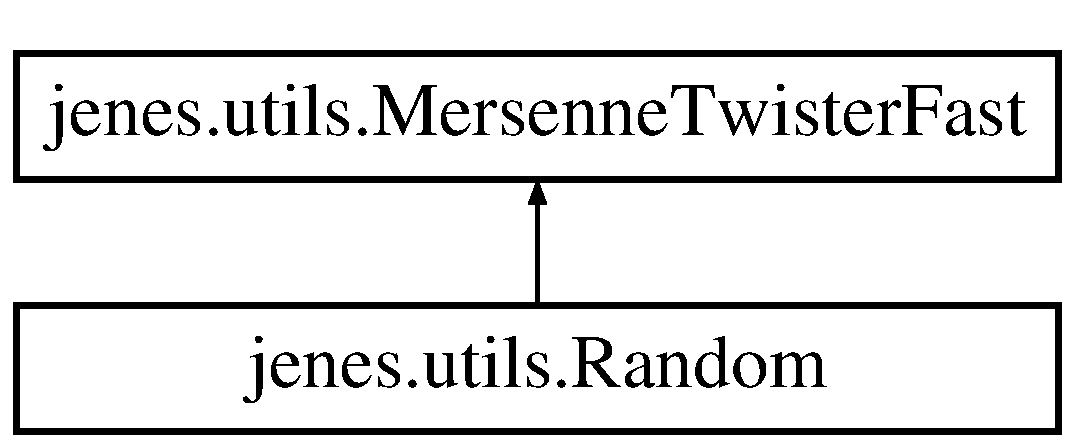
\includegraphics[height=2cm]{classjenes_1_1utils_1_1_random}
\end{center}
\end{figure}
\subsection*{Public Member Functions}
\begin{CompactItemize}
\item 
final void \hyperlink{classjenes_1_1utils_1_1_random_6eec3abcf133f7ce43d6a13441523a01}{setTimeSeed} ()
\item 
final void \hyperlink{classjenes_1_1utils_1_1_random_484017ff9c5473f7fc3fc7b52cb92433}{setStandardSeed} ()
\item 
long \hyperlink{classjenes_1_1utils_1_1_random_55f9b0a836c137e520658f55ad806859}{getSeed} ()
\item 
final double \hyperlink{classjenes_1_1utils_1_1_random_be2919ddf9245e0576591fa0ea26593f}{nextDouble} (final double bound)
\item 
final double \hyperlink{classjenes_1_1utils_1_1_random_19babaa9c19de0243430cef2c445df9c}{nextDouble} (final double lowerBound, final double upperBound)
\item 
final int \hyperlink{classjenes_1_1utils_1_1_random_b066d2d2f6d32c89598c552a9dadedc0}{nextInt} (final int lowerBound, final int upperBound)
\item 
final boolean \hyperlink{classjenes_1_1utils_1_1_random_16e9050a46f8218ec8e0f73c6456a5db}{nextBoolean} (final double coin)
\end{CompactItemize}
\subsection*{Static Public Member Functions}
\begin{CompactItemize}
\item 
static \hyperlink{classjenes_1_1utils_1_1_random}{Random} \hyperlink{classjenes_1_1utils_1_1_random_a8b8341f82ccf69de0b44c9f6f174820}{getInstance} ()
\item 
static \hyperlink{classjenes_1_1utils_1_1_random}{Random} \hyperlink{classjenes_1_1utils_1_1_random_83dd69fffe081a48e58702c0f118b12e}{getInstance} (long seed)
\end{CompactItemize}
\subsection*{Static Public Attributes}
\begin{CompactItemize}
\item 
static final long \hyperlink{classjenes_1_1utils_1_1_random_ee05c4e6476472dc9dc02d2fd94061b5}{STANDARD\_\-SEED} = 4357
\end{CompactItemize}


\subsection{Detailed Description}
This class provides the random generator used by JENES. 

\hyperlink{classjenes_1_1utils_1_1_random}{Random} extends the \hyperlink{classjenes_1_1utils_1_1_mersenne_twister_fast}{MersenneTwisterFast} class with some methods useful to JENES for obtaining values within a range.  

\hyperlink{classjenes_1_1utils_1_1_random}{Random} implements the singleton design pattern, thus only one instance of \hyperlink{classjenes_1_1utils_1_1_random}{Random} is available and retrieved by invoking the method \hyperlink{classjenes_1_1utils_1_1_random_a8b8341f82ccf69de0b44c9f6f174820}{getInstance()}.  

The random sequence is controlled by the seed. The standard seed assures that the same sequence of random values is produced by different runs. The time based seed, assures that the sequences varies run by run. 

\begin{Desc}
\item[Version:]1.2 \end{Desc}
\begin{Desc}
\item[Since:]1.0 \end{Desc}


\subsection{Member Function Documentation}
\hypertarget{classjenes_1_1utils_1_1_random_a8b8341f82ccf69de0b44c9f6f174820}{
\index{jenes::utils::Random@{jenes::utils::Random}!getInstance@{getInstance}}
\index{getInstance@{getInstance}!jenes::utils::Random@{jenes::utils::Random}}
\subsubsection[getInstance]{\setlength{\rightskip}{0pt plus 5cm}static {\bf Random} jenes.utils.Random.getInstance ()\hspace{0.3cm}{\tt  \mbox{[}static\mbox{]}}}}
\label{classjenes_1_1utils_1_1_random_a8b8341f82ccf69de0b44c9f6f174820}


Returns the \hyperlink{classjenes_1_1utils_1_1_random}{Random} singleton. At the first invocation the \hyperlink{classjenes_1_1utils_1_1_random}{Random} object is instantiated.

\begin{Desc}
\item[Returns:]the \hyperlink{classjenes_1_1utils_1_1_random}{Random} instance \end{Desc}
\hypertarget{classjenes_1_1utils_1_1_random_83dd69fffe081a48e58702c0f118b12e}{
\index{jenes::utils::Random@{jenes::utils::Random}!getInstance@{getInstance}}
\index{getInstance@{getInstance}!jenes::utils::Random@{jenes::utils::Random}}
\subsubsection[getInstance]{\setlength{\rightskip}{0pt plus 5cm}static {\bf Random} jenes.utils.Random.getInstance (long {\em seed})\hspace{0.3cm}{\tt  \mbox{[}static\mbox{]}}}}
\label{classjenes_1_1utils_1_1_random_83dd69fffe081a48e58702c0f118b12e}


Returns the \hyperlink{classjenes_1_1utils_1_1_random}{Random} sigleton imposing the seed given as argument \begin{Desc}
\item[Parameters:]
\begin{description}
\item[{\em seed}]\end{description}
\end{Desc}
\begin{Desc}
\item[Returns:]\end{Desc}
\hypertarget{classjenes_1_1utils_1_1_random_6eec3abcf133f7ce43d6a13441523a01}{
\index{jenes::utils::Random@{jenes::utils::Random}!setTimeSeed@{setTimeSeed}}
\index{setTimeSeed@{setTimeSeed}!jenes::utils::Random@{jenes::utils::Random}}
\subsubsection[setTimeSeed]{\setlength{\rightskip}{0pt plus 5cm}final void jenes.utils.Random.setTimeSeed ()}}
\label{classjenes_1_1utils_1_1_random_6eec3abcf133f7ce43d6a13441523a01}


Sets the current time as \hyperlink{classjenes_1_1utils_1_1_random}{Random} seed. This method will make the \hyperlink{classjenes_1_1utils_1_1_random}{Random} sequence of values different run by run. \hypertarget{classjenes_1_1utils_1_1_random_484017ff9c5473f7fc3fc7b52cb92433}{
\index{jenes::utils::Random@{jenes::utils::Random}!setStandardSeed@{setStandardSeed}}
\index{setStandardSeed@{setStandardSeed}!jenes::utils::Random@{jenes::utils::Random}}
\subsubsection[setStandardSeed]{\setlength{\rightskip}{0pt plus 5cm}final void jenes.utils.Random.setStandardSeed ()}}
\label{classjenes_1_1utils_1_1_random_484017ff9c5473f7fc3fc7b52cb92433}


Sets the stardard value as \hyperlink{classjenes_1_1utils_1_1_random}{Random} seed. This method will assure the \hyperlink{classjenes_1_1utils_1_1_random}{Random} sequence of values will not change by run. It should be used for debugging purpose only. \hypertarget{classjenes_1_1utils_1_1_random_55f9b0a836c137e520658f55ad806859}{
\index{jenes::utils::Random@{jenes::utils::Random}!getSeed@{getSeed}}
\index{getSeed@{getSeed}!jenes::utils::Random@{jenes::utils::Random}}
\subsubsection[getSeed]{\setlength{\rightskip}{0pt plus 5cm}long jenes.utils.Random.getSeed ()}}
\label{classjenes_1_1utils_1_1_random_55f9b0a836c137e520658f55ad806859}


Return the current seed used for random \begin{Desc}
\item[Returns:]\end{Desc}


Reimplemented from \hyperlink{classjenes_1_1utils_1_1_mersenne_twister_fast_88963c0469e0bad7a1834469cf0f7a10}{jenes.utils.MersenneTwisterFast}.\hypertarget{classjenes_1_1utils_1_1_random_be2919ddf9245e0576591fa0ea26593f}{
\index{jenes::utils::Random@{jenes::utils::Random}!nextDouble@{nextDouble}}
\index{nextDouble@{nextDouble}!jenes::utils::Random@{jenes::utils::Random}}
\subsubsection[nextDouble]{\setlength{\rightskip}{0pt plus 5cm}final double jenes.utils.Random.nextDouble (final double {\em bound})}}
\label{classjenes_1_1utils_1_1_random_be2919ddf9245e0576591fa0ea26593f}


Returns a random double uniformly distributed within the interval \mbox{[}0,bound\mbox{[}. Please note that bound is excluded. 

\begin{Desc}
\item[Parameters:]
\begin{description}
\item[{\em bound}]the upper bound \end{description}
\end{Desc}
\begin{Desc}
\item[Returns:]a random double uniformly distributed within \mbox{[}0,bound\mbox{[} \end{Desc}
\hypertarget{classjenes_1_1utils_1_1_random_19babaa9c19de0243430cef2c445df9c}{
\index{jenes::utils::Random@{jenes::utils::Random}!nextDouble@{nextDouble}}
\index{nextDouble@{nextDouble}!jenes::utils::Random@{jenes::utils::Random}}
\subsubsection[nextDouble]{\setlength{\rightskip}{0pt plus 5cm}final double jenes.utils.Random.nextDouble (final double {\em lowerBound}, \/  final double {\em upperBound})}}
\label{classjenes_1_1utils_1_1_random_19babaa9c19de0243430cef2c445df9c}


Returns a double uniformly distributed within the interval \mbox{[}lowerBound,upperBound\mbox{[}. Please note that the upperBound is excluded. 

\begin{Desc}
\item[Parameters:]
\begin{description}
\item[{\em lowerBound}]the interval lower bound \item[{\em upperBound}]the interval upper bound \end{description}
\end{Desc}
\begin{Desc}
\item[Returns:]a double uniformly distributed within \mbox{[}lowerBound,upperBound\mbox{[} \end{Desc}
\hypertarget{classjenes_1_1utils_1_1_random_b066d2d2f6d32c89598c552a9dadedc0}{
\index{jenes::utils::Random@{jenes::utils::Random}!nextInt@{nextInt}}
\index{nextInt@{nextInt}!jenes::utils::Random@{jenes::utils::Random}}
\subsubsection[nextInt]{\setlength{\rightskip}{0pt plus 5cm}final int jenes.utils.Random.nextInt (final int {\em lowerBound}, \/  final int {\em upperBound})}}
\label{classjenes_1_1utils_1_1_random_b066d2d2f6d32c89598c552a9dadedc0}


Returns a random integer drawn uniformly in the interval \mbox{[}lowerBound, upperBound\mbox{[}. Please note that upperBound is excluded. Thus the integer is between lowerBound and upperBound-1. 

\begin{Desc}
\item[Parameters:]
\begin{description}
\item[{\em lowerBound}]the interval lower bound \item[{\em upperBound}]the interval upper bound \end{description}
\end{Desc}
\begin{Desc}
\item[Returns:]an integer drawn uniformly from lowerBound to upperBound-1. \end{Desc}
\hypertarget{classjenes_1_1utils_1_1_random_16e9050a46f8218ec8e0f73c6456a5db}{
\index{jenes::utils::Random@{jenes::utils::Random}!nextBoolean@{nextBoolean}}
\index{nextBoolean@{nextBoolean}!jenes::utils::Random@{jenes::utils::Random}}
\subsubsection[nextBoolean]{\setlength{\rightskip}{0pt plus 5cm}final boolean jenes.utils.Random.nextBoolean (final double {\em coin})}}
\label{classjenes_1_1utils_1_1_random_16e9050a46f8218ec8e0f73c6456a5db}


Returns a random boolean value. 

\begin{Desc}
\item[Parameters:]
\begin{description}
\item[{\em coin}]the probability to have a true value \end{description}
\end{Desc}
\begin{Desc}
\item[Returns:]a boolean value \end{Desc}


\subsection{Member Data Documentation}
\hypertarget{classjenes_1_1utils_1_1_random_ee05c4e6476472dc9dc02d2fd94061b5}{
\index{jenes::utils::Random@{jenes::utils::Random}!STANDARD\_\-SEED@{STANDARD\_\-SEED}}
\index{STANDARD\_\-SEED@{STANDARD\_\-SEED}!jenes::utils::Random@{jenes::utils::Random}}
\subsubsection[STANDARD\_\-SEED]{\setlength{\rightskip}{0pt plus 5cm}final long {\bf jenes.utils.Random.STANDARD\_\-SEED} = 4357\hspace{0.3cm}{\tt  \mbox{[}static\mbox{]}}}}
\label{classjenes_1_1utils_1_1_random_ee05c4e6476472dc9dc02d2fd94061b5}


The seed used as default 

The documentation for this class was generated from the following file:\begin{CompactItemize}
\item 
src/jenes/utils/Random.java\end{CompactItemize}

\hypertarget{classjenes_1_1stage_1_1operator_1_1common_1_1_rank_scaling_3_01_t_01extends_01_chromosome_01_4}{
\section{jenes.stage.operator.common.RankScaling$<$ T extends Chromosome $>$ Class Reference}
\label{classjenes_1_1stage_1_1operator_1_1common_1_1_rank_scaling_3_01_t_01extends_01_chromosome_01_4}\index{jenes::stage::operator::common::RankScaling$<$ T extends Chromosome $>$@{jenes::stage::operator::common::RankScaling$<$ T extends Chromosome $>$}}
}
Inherits jenes::stage::operator::Scaling$<$ T $>$.

\subsection*{Public Member Functions}
\begin{CompactItemize}
\item 
\hypertarget{classjenes_1_1stage_1_1operator_1_1common_1_1_rank_scaling_3_01_t_01extends_01_chromosome_01_4_8158f18c672b8764a11ba70a52514132}{
void \textbf{scale} (Population$<$ T $>$ pop)}
\label{classjenes_1_1stage_1_1operator_1_1common_1_1_rank_scaling_3_01_t_01extends_01_chromosome_01_4_8158f18c672b8764a11ba70a52514132}

\end{CompactItemize}


\subsection{Detailed Description}
This operator implements the rank scaling. Rank scaling re-assigns the rank as fitness value to indiduals. The operator is compatible with multi-objective optimization. In that case, rank is in turn computed for each each objective.

\begin{Desc}
\item[Version:]2.0 \end{Desc}
\begin{Desc}
\item[Since:]2.0 \end{Desc}


The documentation for this class was generated from the following file:\begin{CompactItemize}
\item 
src/jenes/stage/operator/common/RankScaling.java\end{CompactItemize}

\hypertarget{classjenes_1_1stage_1_1operator_1_1common_1_1_roulette_wheel_selector_3_01_t_01extends_01_chromosome_01_4}{
\section{jenes.stage.operator.common.RouletteWheelSelector$<$ T extends Chromosome $>$ Class Reference}
\label{classjenes_1_1stage_1_1operator_1_1common_1_1_roulette_wheel_selector_3_01_t_01extends_01_chromosome_01_4}\index{jenes::stage::operator::common::RouletteWheelSelector$<$ T extends Chromosome $>$@{jenes::stage::operator::common::RouletteWheelSelector$<$ T extends Chromosome $>$}}
}
Inherits jenes::stage::operator::Selector$<$ T $>$.

\subsection*{Protected Member Functions}
\begin{CompactItemize}
\item 
\hypertarget{classjenes_1_1stage_1_1operator_1_1common_1_1_roulette_wheel_selector_3_01_t_01extends_01_chromosome_01_4_13a6b76fa77779367d05a063ff6191bf}{
void \textbf{preSelect} (Population$<$ T $>$ pop, Filter filter)}
\label{classjenes_1_1stage_1_1operator_1_1common_1_1_roulette_wheel_selector_3_01_t_01extends_01_chromosome_01_4_13a6b76fa77779367d05a063ff6191bf}

\item 
\hypertarget{classjenes_1_1stage_1_1operator_1_1common_1_1_roulette_wheel_selector_3_01_t_01extends_01_chromosome_01_4_d74c66e053cb97c75ce8a9f78a8208e5}{
Individual$<$ T $>$ \textbf{select} (List$<$ Individual$<$ T $>$$>$ list)}
\label{classjenes_1_1stage_1_1operator_1_1common_1_1_roulette_wheel_selector_3_01_t_01extends_01_chromosome_01_4_d74c66e053cb97c75ce8a9f78a8208e5}

\end{CompactItemize}
\subsection*{Package Attributes}
\begin{CompactItemize}
\item 
\hypertarget{classjenes_1_1stage_1_1operator_1_1common_1_1_roulette_wheel_selector_3_01_t_01extends_01_chromosome_01_4_c030f795440f2d69c4e08f80219cda30}{
double\mbox{[}$\,$\mbox{]} \textbf{cumulativeFit} = null}
\label{classjenes_1_1stage_1_1operator_1_1common_1_1_roulette_wheel_selector_3_01_t_01extends_01_chromosome_01_4_c030f795440f2d69c4e08f80219cda30}

\item 
\hypertarget{classjenes_1_1stage_1_1operator_1_1common_1_1_roulette_wheel_selector_3_01_t_01extends_01_chromosome_01_4_f64e3d25c886903470c3e188b287af4c}{
double\mbox{[}$\,$\mbox{]} \textbf{fit} = null}
\label{classjenes_1_1stage_1_1operator_1_1common_1_1_roulette_wheel_selector_3_01_t_01extends_01_chromosome_01_4_f64e3d25c886903470c3e188b287af4c}

\item 
\hypertarget{classjenes_1_1stage_1_1operator_1_1common_1_1_roulette_wheel_selector_3_01_t_01extends_01_chromosome_01_4_c073a280077bd972cab00cd2608ae415}{
double\mbox{[}$\,$\mbox{]} \textbf{partialFit} = null}
\label{classjenes_1_1stage_1_1operator_1_1common_1_1_roulette_wheel_selector_3_01_t_01extends_01_chromosome_01_4_c073a280077bd972cab00cd2608ae415}

\end{CompactItemize}


\subsection{Detailed Description}
A classic roulette wheel selection operator. If s if the input population size, s individuals will be selected. The best ones have a higher selection probability. A \hyperlink{}{preSelect(Population)} method is useful to set up the selection state according to the population state to undergo at the selection process. 

\begin{Desc}
\item[Parameters:]
\begin{description}
\item[{\em $<$T$>$}]The class of chromosomes to work with.\end{description}
\end{Desc}
\begin{Desc}
\item[Version:]2.0 \end{Desc}
\begin{Desc}
\item[Since:]1.0\end{Desc}
\begin{Desc}
\item[See also:]Individual 

Population \end{Desc}


The documentation for this class was generated from the following file:\begin{CompactItemize}
\item 
src/jenes/stage/operator/common/RouletteWheelSelector.java\end{CompactItemize}

\hypertarget{classjenes_1_1utils_1_1multitasking_1_1_runner}{
\section{jenes.utils.multitasking.Runner Class Reference}
\label{classjenes_1_1utils_1_1multitasking_1_1_runner}\index{jenes::utils::multitasking::Runner@{jenes::utils::multitasking::Runner}}
}
Inheritance diagram for jenes.utils.multitasking.Runner::\begin{figure}[H]
\begin{center}
\leavevmode
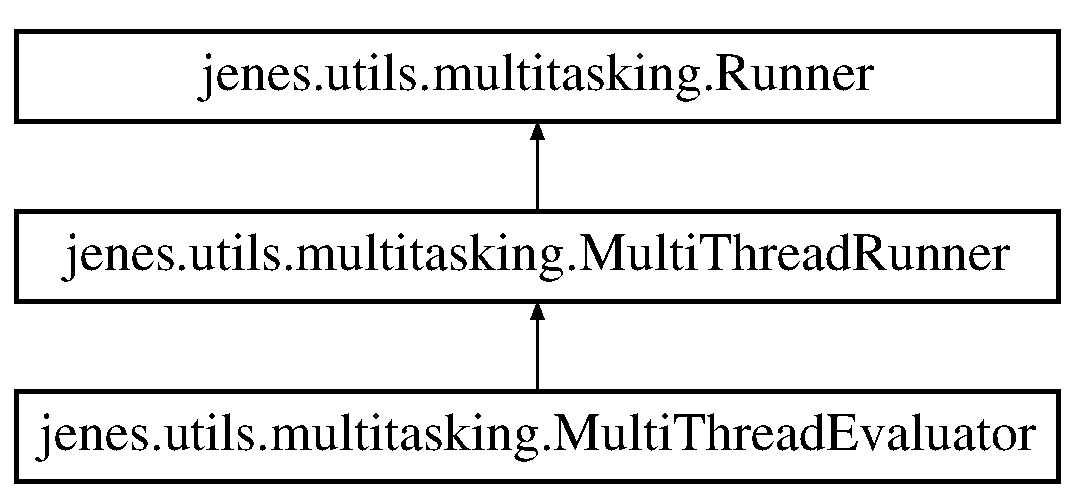
\includegraphics[height=3cm]{classjenes_1_1utils_1_1multitasking_1_1_runner}
\end{center}
\end{figure}
\subsection*{Public Member Functions}
\begin{CompactItemize}
\item 
final void \hyperlink{classjenes_1_1utils_1_1multitasking_1_1_runner_24d074cbd5140cd8bc65623fa1961f39}{execute} (GeneticAlgorithm \hyperlink{classjenes_1_1utils_1_1multitasking_1_1_runner_699ccf526b6116f97abc09e4ce390c89}{algorithm}, boolean restart)
\item 
final void \hyperlink{classjenes_1_1utils_1_1multitasking_1_1_runner_e222d69f44508fc432c05074272e0ae3}{execute} (GeneticAlgorithm algoritm)
\item 
final void \hyperlink{classjenes_1_1utils_1_1multitasking_1_1_runner_7205f2d93d68f40e3e87dccf92cc3720}{execute} (GeneticAlgorithm \hyperlink{classjenes_1_1utils_1_1multitasking_1_1_runner_699ccf526b6116f97abc09e4ce390c89}{algorithm}, Population$<$?$>$ initialPopulation)
\item 
GeneticAlgorithm \hyperlink{classjenes_1_1utils_1_1multitasking_1_1_runner_462a121a840bbf06593bbd7da219d8b9}{getGeneticAlgorithm} ()
\item 
void \hyperlink{classjenes_1_1utils_1_1multitasking_1_1_runner_dad9fb400d736e55bcd3dfdf07742437}{setAlgorithm} (GeneticAlgorithm \hyperlink{classjenes_1_1utils_1_1multitasking_1_1_runner_699ccf526b6116f97abc09e4ce390c89}{algorithm})
\item 
void \hyperlink{classjenes_1_1utils_1_1multitasking_1_1_runner_5dc1ed49495150ff26ec5194010b00e4}{start} (boolean reset)
\item 
void \hyperlink{classjenes_1_1utils_1_1multitasking_1_1_runner_4c4d4a0cd7aec110d60da5c660903398}{onInit} ()
\item 
void \hyperlink{classjenes_1_1utils_1_1multitasking_1_1_runner_c89e8ac54daba2e326e687662ff9f7b0}{stop} ()
\item 
void \hyperlink{classjenes_1_1utils_1_1multitasking_1_1_runner_6ec13cf0fb2ff03461a3a397421505cf}{onEvaluationBegin} (Population pop, boolean forced)
\item 
void \hyperlink{classjenes_1_1utils_1_1multitasking_1_1_runner_82c84ad942296d62849248b107ec3a2c}{onEvaluationEnd} ()
\item 
abstract void \hyperlink{classjenes_1_1utils_1_1multitasking_1_1_runner_250c5e0ffdb86ef0bb0e78e625a449e7}{evaluateIndividual} (Individual individual)
\end{CompactItemize}
\subsection*{Protected Attributes}
\begin{CompactItemize}
\item 
GeneticAlgorithm \hyperlink{classjenes_1_1utils_1_1multitasking_1_1_runner_699ccf526b6116f97abc09e4ce390c89}{algorithm}
\end{CompactItemize}


\subsection{Detailed Description}
The \hyperlink{classjenes_1_1utils_1_1multitasking_1_1_runner}{Runner} is the abstraction of an execution enviroinment per Jenes. By now this approach has been used to parallelize the fitness evaluation step. The programmer have to override the default call-backs than use \hyperlink{}{execute(jenes.GeneticAlgorithm)} or \hyperlink{}{execute(jenes.GeneticAlgorithm, boolean)} to activate Genetic Algorithm to start evolving in the enviroinment.

\begin{Desc}
\item[Since:]2.0 \end{Desc}


\subsection{Member Function Documentation}
\hypertarget{classjenes_1_1utils_1_1multitasking_1_1_runner_24d074cbd5140cd8bc65623fa1961f39}{
\index{jenes::utils::multitasking::Runner@{jenes::utils::multitasking::Runner}!execute@{execute}}
\index{execute@{execute}!jenes::utils::multitasking::Runner@{jenes::utils::multitasking::Runner}}
\subsubsection[execute]{\setlength{\rightskip}{0pt plus 5cm}final void jenes.utils.multitasking.Runner.execute (GeneticAlgorithm {\em algorithm}, \/  boolean {\em restart})}}
\label{classjenes_1_1utils_1_1multitasking_1_1_runner_24d074cbd5140cd8bc65623fa1961f39}


Start evolving the algorithm given as parameter in this enviroinment by applying to specificated restart flag.

\begin{Desc}
\item[Parameters:]
\begin{description}
\item[{\em algorithm}]the algorithm to evolve \item[{\em restart}]{\tt restart} flag to pass to \hyperlink{}{GeneticAlgorithm\#evolve(boolean)} \end{description}
\end{Desc}
\hypertarget{classjenes_1_1utils_1_1multitasking_1_1_runner_e222d69f44508fc432c05074272e0ae3}{
\index{jenes::utils::multitasking::Runner@{jenes::utils::multitasking::Runner}!execute@{execute}}
\index{execute@{execute}!jenes::utils::multitasking::Runner@{jenes::utils::multitasking::Runner}}
\subsubsection[execute]{\setlength{\rightskip}{0pt plus 5cm}final void jenes.utils.multitasking.Runner.execute (GeneticAlgorithm {\em algoritm})}}
\label{classjenes_1_1utils_1_1multitasking_1_1_runner_e222d69f44508fc432c05074272e0ae3}


Start evolving the algorithm given as argument restarting its state \begin{Desc}
\item[Parameters:]
\begin{description}
\item[{\em algoritm}]the algorithm to evolve \end{description}
\end{Desc}
\begin{Desc}
\item[See also:]\hyperlink{classjenes_1_1utils_1_1multitasking_1_1_runner_24d074cbd5140cd8bc65623fa1961f39}{execute}(jenes.GeneticAlgorithm, boolean) \end{Desc}
\hypertarget{classjenes_1_1utils_1_1multitasking_1_1_runner_7205f2d93d68f40e3e87dccf92cc3720}{
\index{jenes::utils::multitasking::Runner@{jenes::utils::multitasking::Runner}!execute@{execute}}
\index{execute@{execute}!jenes::utils::multitasking::Runner@{jenes::utils::multitasking::Runner}}
\subsubsection[execute]{\setlength{\rightskip}{0pt plus 5cm}final void jenes.utils.multitasking.Runner.execute (GeneticAlgorithm {\em algorithm}, \/  Population$<$?$>$ {\em initialPopulation})}}
\label{classjenes_1_1utils_1_1multitasking_1_1_runner_7205f2d93d68f40e3e87dccf92cc3720}


Start evolving the algorithm given and adopting as initial population the one passed as argument \begin{Desc}
\item[Parameters:]
\begin{description}
\item[{\em algorithm}]\item[{\em initialPopulation}]\end{description}
\end{Desc}
\hypertarget{classjenes_1_1utils_1_1multitasking_1_1_runner_462a121a840bbf06593bbd7da219d8b9}{
\index{jenes::utils::multitasking::Runner@{jenes::utils::multitasking::Runner}!getGeneticAlgorithm@{getGeneticAlgorithm}}
\index{getGeneticAlgorithm@{getGeneticAlgorithm}!jenes::utils::multitasking::Runner@{jenes::utils::multitasking::Runner}}
\subsubsection[getGeneticAlgorithm]{\setlength{\rightskip}{0pt plus 5cm}GeneticAlgorithm jenes.utils.multitasking.Runner.getGeneticAlgorithm ()}}
\label{classjenes_1_1utils_1_1multitasking_1_1_runner_462a121a840bbf06593bbd7da219d8b9}


Return the Genetic Algorithm currently in execution in this enviroinment \begin{Desc}
\item[Returns:]\end{Desc}
\hypertarget{classjenes_1_1utils_1_1multitasking_1_1_runner_dad9fb400d736e55bcd3dfdf07742437}{
\index{jenes::utils::multitasking::Runner@{jenes::utils::multitasking::Runner}!setAlgorithm@{setAlgorithm}}
\index{setAlgorithm@{setAlgorithm}!jenes::utils::multitasking::Runner@{jenes::utils::multitasking::Runner}}
\subsubsection[setAlgorithm]{\setlength{\rightskip}{0pt plus 5cm}void jenes.utils.multitasking.Runner.setAlgorithm (GeneticAlgorithm {\em algorithm})}}
\label{classjenes_1_1utils_1_1multitasking_1_1_runner_dad9fb400d736e55bcd3dfdf07742437}


Set the Genetic Algorithm to the runner. This value will be overridden when execute is called. \begin{Desc}
\item[Parameters:]
\begin{description}
\item[{\em algorithm}]\end{description}
\end{Desc}
\hypertarget{classjenes_1_1utils_1_1multitasking_1_1_runner_5dc1ed49495150ff26ec5194010b00e4}{
\index{jenes::utils::multitasking::Runner@{jenes::utils::multitasking::Runner}!start@{start}}
\index{start@{start}!jenes::utils::multitasking::Runner@{jenes::utils::multitasking::Runner}}
\subsubsection[start]{\setlength{\rightskip}{0pt plus 5cm}void jenes.utils.multitasking.Runner.start (boolean {\em reset})}}
\label{classjenes_1_1utils_1_1multitasking_1_1_runner_5dc1ed49495150ff26ec5194010b00e4}


Call-back invoked by \hyperlink{}{GeneticAlgorithm\#start(boolean)} \begin{Desc}
\item[Parameters:]
\begin{description}
\item[{\em reset}]\end{description}
\end{Desc}


Reimplemented in \hyperlink{classjenes_1_1utils_1_1multitasking_1_1_multi_thread_runner_52fc59a28c3187e84b871b9b823b7f43}{jenes.utils.multitasking.MultiThreadRunner}.\hypertarget{classjenes_1_1utils_1_1multitasking_1_1_runner_4c4d4a0cd7aec110d60da5c660903398}{
\index{jenes::utils::multitasking::Runner@{jenes::utils::multitasking::Runner}!onInit@{onInit}}
\index{onInit@{onInit}!jenes::utils::multitasking::Runner@{jenes::utils::multitasking::Runner}}
\subsubsection[onInit]{\setlength{\rightskip}{0pt plus 5cm}void jenes.utils.multitasking.Runner.onInit ()}}
\label{classjenes_1_1utils_1_1multitasking_1_1_runner_4c4d4a0cd7aec110d60da5c660903398}


Call-back invoked soon before \hyperlink{}{GeneticAlgorithm\#onInit(long)} \hypertarget{classjenes_1_1utils_1_1multitasking_1_1_runner_c89e8ac54daba2e326e687662ff9f7b0}{
\index{jenes::utils::multitasking::Runner@{jenes::utils::multitasking::Runner}!stop@{stop}}
\index{stop@{stop}!jenes::utils::multitasking::Runner@{jenes::utils::multitasking::Runner}}
\subsubsection[stop]{\setlength{\rightskip}{0pt plus 5cm}void jenes.utils.multitasking.Runner.stop ()}}
\label{classjenes_1_1utils_1_1multitasking_1_1_runner_c89e8ac54daba2e326e687662ff9f7b0}


Call-back called soon after \hyperlink{}{GeneticAlgorithm\#onStop(long)} 

Reimplemented in \hyperlink{classjenes_1_1utils_1_1multitasking_1_1_multi_thread_runner_5f00a9b63ff1322d586ad62ec060d597}{jenes.utils.multitasking.MultiThreadRunner}.\hypertarget{classjenes_1_1utils_1_1multitasking_1_1_runner_6ec13cf0fb2ff03461a3a397421505cf}{
\index{jenes::utils::multitasking::Runner@{jenes::utils::multitasking::Runner}!onEvaluationBegin@{onEvaluationBegin}}
\index{onEvaluationBegin@{onEvaluationBegin}!jenes::utils::multitasking::Runner@{jenes::utils::multitasking::Runner}}
\subsubsection[onEvaluationBegin]{\setlength{\rightskip}{0pt plus 5cm}void jenes.utils.multitasking.Runner.onEvaluationBegin (Population {\em pop}, \/  boolean {\em forced})}}
\label{classjenes_1_1utils_1_1multitasking_1_1_runner_6ec13cf0fb2ff03461a3a397421505cf}


Call-back invoked soon before the \hyperlink{}{Population} evaluation starts using the default \hyperlink{}{Fitness} defined per \hyperlink{}{GeneticAlgorithm}

\begin{Desc}
\item[Parameters:]
\begin{description}
\item[{\em pop}]the population that will be evaluated \item[{\em forced}]if each individual of the population will be forced to be evaluated \end{description}
\end{Desc}


Reimplemented in \hyperlink{classjenes_1_1utils_1_1multitasking_1_1_multi_thread_evaluator_2a9d9427ca8c2b8a9dfc541c85bada42}{jenes.utils.multitasking.MultiThreadEvaluator}.\hypertarget{classjenes_1_1utils_1_1multitasking_1_1_runner_82c84ad942296d62849248b107ec3a2c}{
\index{jenes::utils::multitasking::Runner@{jenes::utils::multitasking::Runner}!onEvaluationEnd@{onEvaluationEnd}}
\index{onEvaluationEnd@{onEvaluationEnd}!jenes::utils::multitasking::Runner@{jenes::utils::multitasking::Runner}}
\subsubsection[onEvaluationEnd]{\setlength{\rightskip}{0pt plus 5cm}void jenes.utils.multitasking.Runner.onEvaluationEnd ()}}
\label{classjenes_1_1utils_1_1multitasking_1_1_runner_82c84ad942296d62849248b107ec3a2c}


Call-back invoked soon after the evaluation phase has been performed. \par
 WARNING: the method is called before the elapsed time per evaluation is computed so a huge work could affect measurements. 

Reimplemented in \hyperlink{classjenes_1_1utils_1_1multitasking_1_1_multi_thread_evaluator_3cd56b43989da43e4b3c2b79260d5f5f}{jenes.utils.multitasking.MultiThreadEvaluator}.\hypertarget{classjenes_1_1utils_1_1multitasking_1_1_runner_250c5e0ffdb86ef0bb0e78e625a449e7}{
\index{jenes::utils::multitasking::Runner@{jenes::utils::multitasking::Runner}!evaluateIndividual@{evaluateIndividual}}
\index{evaluateIndividual@{evaluateIndividual}!jenes::utils::multitasking::Runner@{jenes::utils::multitasking::Runner}}
\subsubsection[evaluateIndividual]{\setlength{\rightskip}{0pt plus 5cm}abstract void jenes.utils.multitasking.Runner.evaluateIndividual (Individual {\em individual})\hspace{0.3cm}{\tt  \mbox{[}pure virtual\mbox{]}}}}
\label{classjenes_1_1utils_1_1multitasking_1_1_runner_250c5e0ffdb86ef0bb0e78e625a449e7}


Call-back invoked in substitution to \hyperlink{}{GeneticAlgorithm\#evaluateIndividual(jenes.population.Individual)} \begin{Desc}
\item[Parameters:]
\begin{description}
\item[{\em individual}]\end{description}
\end{Desc}


Implemented in \hyperlink{classjenes_1_1utils_1_1multitasking_1_1_multi_thread_evaluator_d99c13b137f1089a9f30377548b42e25}{jenes.utils.multitasking.MultiThreadEvaluator}.

\subsection{Member Data Documentation}
\hypertarget{classjenes_1_1utils_1_1multitasking_1_1_runner_699ccf526b6116f97abc09e4ce390c89}{
\index{jenes::utils::multitasking::Runner@{jenes::utils::multitasking::Runner}!algorithm@{algorithm}}
\index{algorithm@{algorithm}!jenes::utils::multitasking::Runner@{jenes::utils::multitasking::Runner}}
\subsubsection[algorithm]{\setlength{\rightskip}{0pt plus 5cm}GeneticAlgorithm {\bf jenes.utils.multitasking.Runner.algorithm}\hspace{0.3cm}{\tt  \mbox{[}protected\mbox{]}}}}
\label{classjenes_1_1utils_1_1multitasking_1_1_runner_699ccf526b6116f97abc09e4ce390c89}


The algorithm to evolve in the enviroinment 

The documentation for this class was generated from the following file:\begin{CompactItemize}
\item 
src/jenes/utils/multitasking/Runner.java\end{CompactItemize}

\hypertarget{classjenes_1_1stage_1_1operator_1_1_scaling_3_01_t_01extends_01_chromosome_01_4}{
\section{jenes.stage.operator.Scaling$<$ T extends Chromosome $>$ Class Reference}
\label{classjenes_1_1stage_1_1operator_1_1_scaling_3_01_t_01extends_01_chromosome_01_4}\index{jenes::stage::operator::Scaling$<$ T extends Chromosome $>$@{jenes::stage::operator::Scaling$<$ T extends Chromosome $>$}}
}
\subsection*{Public Member Functions}
\begin{CompactItemize}
\item 
\hyperlink{classjenes_1_1stage_1_1operator_1_1_scaling_3_01_t_01extends_01_chromosome_01_4_04089dfb0f712c85ca27fdbab69a5b9e}{Scaling} ()
\item 
\hypertarget{classjenes_1_1stage_1_1operator_1_1_scaling_3_01_t_01extends_01_chromosome_01_4_1577b3956323b5110e4c740ccaaa5905}{
final void \textbf{process} (Population$<$ T $>$ in, Population$<$ T $>$ out)  throws StageException }
\label{classjenes_1_1stage_1_1operator_1_1_scaling_3_01_t_01extends_01_chromosome_01_4_1577b3956323b5110e4c740ccaaa5905}

\item 
abstract void \hyperlink{classjenes_1_1stage_1_1operator_1_1_scaling_3_01_t_01extends_01_chromosome_01_4_e72d4b2ab8bd3504471ce67788c841cd}{scale} (Population$<$ T $>$ pop)
\end{CompactItemize}


\subsection{Detailed Description}
This class of operators performs fitness scaling. They can be implemented by overwriting the method {\tt scale}

\begin{Desc}
\item[Version:]2.0 \end{Desc}
\begin{Desc}
\item[Since:]2.0 \end{Desc}


\subsection{Constructor \& Destructor Documentation}
\hypertarget{classjenes_1_1stage_1_1operator_1_1_scaling_3_01_t_01extends_01_chromosome_01_4_04089dfb0f712c85ca27fdbab69a5b9e}{
\index{jenes::stage::operator::Scaling$<$ T extends Chromosome $>$@{jenes::stage::operator::Scaling$<$ T extends Chromosome $>$}!Scaling@{Scaling}}
\index{Scaling@{Scaling}!jenes::stage::operator::Scaling< T extends Chromosome >@{jenes::stage::operator::Scaling$<$ T extends Chromosome $>$}}
\subsubsection[Scaling]{\setlength{\rightskip}{0pt plus 5cm}jenes.stage.operator.Scaling$<$ T extends Chromosome $>$.Scaling ()}}
\label{classjenes_1_1stage_1_1operator_1_1_scaling_3_01_t_01extends_01_chromosome_01_4_04089dfb0f712c85ca27fdbab69a5b9e}


Constructor 

\subsection{Member Function Documentation}
\hypertarget{classjenes_1_1stage_1_1operator_1_1_scaling_3_01_t_01extends_01_chromosome_01_4_e72d4b2ab8bd3504471ce67788c841cd}{
\index{jenes::stage::operator::Scaling$<$ T extends Chromosome $>$@{jenes::stage::operator::Scaling$<$ T extends Chromosome $>$}!scale@{scale}}
\index{scale@{scale}!jenes::stage::operator::Scaling< T extends Chromosome >@{jenes::stage::operator::Scaling$<$ T extends Chromosome $>$}}
\subsubsection[scale]{\setlength{\rightskip}{0pt plus 5cm}abstract void jenes.stage.operator.Scaling$<$ T extends Chromosome $>$.scale (Population$<$ T $>$ {\em pop})\hspace{0.3cm}{\tt  \mbox{[}pure virtual\mbox{]}}}}
\label{classjenes_1_1stage_1_1operator_1_1_scaling_3_01_t_01extends_01_chromosome_01_4_e72d4b2ab8bd3504471ce67788c841cd}


Method used to scale the fitness of indivduals belonging to given {\tt Population} 

\begin{Desc}
\item[Parameters:]
\begin{description}
\item[{\em pop}]population of individuals to scale \end{description}
\end{Desc}


The documentation for this class was generated from the following file:\begin{CompactItemize}
\item 
src/jenes/stage/operator/Scaling.java\end{CompactItemize}

\hypertarget{classjenes_1_1stage_1_1operator_1_1_selector_3_01_t_01extends_01_chromosome_01_4}{
\section{jenes.stage.operator.Selector$<$ T extends Chromosome $>$ Class Reference}
\label{classjenes_1_1stage_1_1operator_1_1_selector_3_01_t_01extends_01_chromosome_01_4}\index{jenes::stage::operator::Selector$<$ T extends Chromosome $>$@{jenes::stage::operator::Selector$<$ T extends Chromosome $>$}}
}
\subsection*{Public Member Functions}
\begin{CompactItemize}
\item 
\hyperlink{classjenes_1_1stage_1_1operator_1_1_selector_3_01_t_01extends_01_chromosome_01_4_83052368d6df966944bc5178f1eebed0}{Selector} ()
\item 
\hyperlink{classjenes_1_1stage_1_1operator_1_1_selector_3_01_t_01extends_01_chromosome_01_4_07f05455c1fabfb8ad3f6468a653aed8}{Selector} (int n)
\item 
final double \hyperlink{classjenes_1_1stage_1_1operator_1_1_selector_3_01_t_01extends_01_chromosome_01_4_6e6f7842d22da347196a8cd772bea0e1}{getMaxIllegalRate} ()
\item 
void \hyperlink{classjenes_1_1stage_1_1operator_1_1_selector_3_01_t_01extends_01_chromosome_01_4_68ffd7e37d617f2f71628ce3659a8457}{setMaxIllegalRate} (double rate)
\item 
final int \hyperlink{classjenes_1_1stage_1_1operator_1_1_selector_3_01_t_01extends_01_chromosome_01_4_17809883b498ec5764c5aa38d04bda8b}{getSelectionRate} ()
\item 
void \hyperlink{classjenes_1_1stage_1_1operator_1_1_selector_3_01_t_01extends_01_chromosome_01_4_a67094343d09f80b0ce35d0f20a517d5}{setSelectionRate} (int n)
\item 
\hypertarget{classjenes_1_1stage_1_1operator_1_1_selector_3_01_t_01extends_01_chromosome_01_4_780969225a2e48774e71af8bd4e0063e}{
void \textbf{init} (GeneticAlgorithm$<$ T $>$ ga)}
\label{classjenes_1_1stage_1_1operator_1_1_selector_3_01_t_01extends_01_chromosome_01_4_780969225a2e48774e71af8bd4e0063e}

\item 
final void \hyperlink{classjenes_1_1stage_1_1operator_1_1_selector_3_01_t_01extends_01_chromosome_01_4_11275bed8b009ece669a5c88c6e10b55}{process} (Population$<$ T $>$ in, Population$<$ T $>$ out)  throws StageException 
\item 
final Individual$<$ T $>$ \hyperlink{classjenes_1_1stage_1_1operator_1_1_selector_3_01_t_01extends_01_chromosome_01_4_9ef7b0bef2ffcb84eeb231ae37ab0239}{select} (Population$<$ T $>$ pop)
\end{CompactItemize}
\subsection*{Static Public Attributes}
\begin{CompactItemize}
\item 
static final double \hyperlink{classjenes_1_1stage_1_1operator_1_1_selector_3_01_t_01extends_01_chromosome_01_4_81263464a18d2ee1ecddf41f2e97fd89}{DEFAULT\_\-MAX\_\-ILLEGAL\_\-RATE} = 0.3
\end{CompactItemize}
\subsection*{Protected Member Functions}
\begin{CompactItemize}
\item 
void \hyperlink{classjenes_1_1stage_1_1operator_1_1_selector_3_01_t_01extends_01_chromosome_01_4_752bf2650cbb6760d2fbb68718d62328}{preSelect} (Population$<$ T $>$ pop, Filter filter)
\item 
abstract Individual$<$ T $>$ \hyperlink{classjenes_1_1stage_1_1operator_1_1_selector_3_01_t_01extends_01_chromosome_01_4_f6cf22a6d6e70ffd74ee1f042a16dcd9}{select} (List$<$ Individual$<$ T $>$$>$ pop)
\end{CompactItemize}
\subsection*{Classes}
\begin{CompactItemize}
\item 
class \hyperlink{classjenes_1_1stage_1_1operator_1_1_selector_3_01_t_01extends_01_chromosome_01_4_1_1_statistics}{Statistics}
\end{CompactItemize}


\subsection{Detailed Description}
A class representing a generic selection operator. 

The actual selector is implemented by subclassing this abstract class and providing the \hyperlink{}{Selector\#select(Population)} and \hyperlink{}{Selector\#preSelect(Population)} method implementations: the former is required to select individuals from the specified \hyperlink{}{Population}; the latter is required to set up the selector state when a new selection begins. 

A \hyperlink{}{Selector\#maxIllegalRate} is specified to obtain a population with a max number of illegal individuals selected. When this threshould is reached, the new illegal selected individuals are not added at the output population, and the selection process is repeated. 

At the start selection time the output population has already the individuals; the individuals selected from the input population have not to be added at the output population: each output population individual is set as the one selected by the input population. 

The output population size will be equal to the input population one; automatically new individuals are added or old ones are deleted to make the sizes equal. 

A \hyperlink{}{Selector.Statistics} is associated to each selector operator.

\begin{Desc}
\item[Parameters:]
\begin{description}
\item[{\em $<$T$>$}]The class of chromosomes to work with.\end{description}
\end{Desc}
\begin{Desc}
\item[Version:]2.0 \end{Desc}
\begin{Desc}
\item[Since:]1.0\end{Desc}
\begin{Desc}
\item[See also:]Individual 

Population \end{Desc}


\subsection{Constructor \& Destructor Documentation}
\hypertarget{classjenes_1_1stage_1_1operator_1_1_selector_3_01_t_01extends_01_chromosome_01_4_83052368d6df966944bc5178f1eebed0}{
\index{jenes::stage::operator::Selector$<$ T extends Chromosome $>$@{jenes::stage::operator::Selector$<$ T extends Chromosome $>$}!Selector@{Selector}}
\index{Selector@{Selector}!jenes::stage::operator::Selector< T extends Chromosome >@{jenes::stage::operator::Selector$<$ T extends Chromosome $>$}}
\subsubsection[Selector]{\setlength{\rightskip}{0pt plus 5cm}jenes.stage.operator.Selector$<$ T extends Chromosome $>$.Selector ()}}
\label{classjenes_1_1stage_1_1operator_1_1_selector_3_01_t_01extends_01_chromosome_01_4_83052368d6df966944bc5178f1eebed0}


Constructs a new Selector operator. \hypertarget{classjenes_1_1stage_1_1operator_1_1_selector_3_01_t_01extends_01_chromosome_01_4_07f05455c1fabfb8ad3f6468a653aed8}{
\index{jenes::stage::operator::Selector$<$ T extends Chromosome $>$@{jenes::stage::operator::Selector$<$ T extends Chromosome $>$}!Selector@{Selector}}
\index{Selector@{Selector}!jenes::stage::operator::Selector< T extends Chromosome >@{jenes::stage::operator::Selector$<$ T extends Chromosome $>$}}
\subsubsection[Selector]{\setlength{\rightskip}{0pt plus 5cm}jenes.stage.operator.Selector$<$ T extends Chromosome $>$.Selector (int {\em n})}}
\label{classjenes_1_1stage_1_1operator_1_1_selector_3_01_t_01extends_01_chromosome_01_4_07f05455c1fabfb8ad3f6468a653aed8}


Constructs a new Selector operator, specifying the number of individuals to select.

\begin{Desc}
\item[Parameters:]
\begin{description}
\item[{\em n}]the number of individuals to select \end{description}
\end{Desc}


\subsection{Member Function Documentation}
\hypertarget{classjenes_1_1stage_1_1operator_1_1_selector_3_01_t_01extends_01_chromosome_01_4_6e6f7842d22da347196a8cd772bea0e1}{
\index{jenes::stage::operator::Selector$<$ T extends Chromosome $>$@{jenes::stage::operator::Selector$<$ T extends Chromosome $>$}!getMaxIllegalRate@{getMaxIllegalRate}}
\index{getMaxIllegalRate@{getMaxIllegalRate}!jenes::stage::operator::Selector< T extends Chromosome >@{jenes::stage::operator::Selector$<$ T extends Chromosome $>$}}
\subsubsection[getMaxIllegalRate]{\setlength{\rightskip}{0pt plus 5cm}final double jenes.stage.operator.Selector$<$ T extends Chromosome $>$.getMaxIllegalRate ()}}
\label{classjenes_1_1stage_1_1operator_1_1_selector_3_01_t_01extends_01_chromosome_01_4_6e6f7842d22da347196a8cd772bea0e1}


Returns the max number of illegal individuals this selector operator can select.

\begin{Desc}
\item[Returns:]the max illegal rate \end{Desc}
\hypertarget{classjenes_1_1stage_1_1operator_1_1_selector_3_01_t_01extends_01_chromosome_01_4_68ffd7e37d617f2f71628ce3659a8457}{
\index{jenes::stage::operator::Selector$<$ T extends Chromosome $>$@{jenes::stage::operator::Selector$<$ T extends Chromosome $>$}!setMaxIllegalRate@{setMaxIllegalRate}}
\index{setMaxIllegalRate@{setMaxIllegalRate}!jenes::stage::operator::Selector< T extends Chromosome >@{jenes::stage::operator::Selector$<$ T extends Chromosome $>$}}
\subsubsection[setMaxIllegalRate]{\setlength{\rightskip}{0pt plus 5cm}void jenes.stage.operator.Selector$<$ T extends Chromosome $>$.setMaxIllegalRate (double {\em rate})}}
\label{classjenes_1_1stage_1_1operator_1_1_selector_3_01_t_01extends_01_chromosome_01_4_68ffd7e37d617f2f71628ce3659a8457}


Sets the max number of illegal individuals this selector operator can select.

\begin{Desc}
\item[Parameters:]
\begin{description}
\item[{\em rate}]the max illegal rate \end{description}
\end{Desc}
\hypertarget{classjenes_1_1stage_1_1operator_1_1_selector_3_01_t_01extends_01_chromosome_01_4_17809883b498ec5764c5aa38d04bda8b}{
\index{jenes::stage::operator::Selector$<$ T extends Chromosome $>$@{jenes::stage::operator::Selector$<$ T extends Chromosome $>$}!getSelectionRate@{getSelectionRate}}
\index{getSelectionRate@{getSelectionRate}!jenes::stage::operator::Selector< T extends Chromosome >@{jenes::stage::operator::Selector$<$ T extends Chromosome $>$}}
\subsubsection[getSelectionRate]{\setlength{\rightskip}{0pt plus 5cm}final int jenes.stage.operator.Selector$<$ T extends Chromosome $>$.getSelectionRate ()}}
\label{classjenes_1_1stage_1_1operator_1_1_selector_3_01_t_01extends_01_chromosome_01_4_17809883b498ec5764c5aa38d04bda8b}


Returns the number of individuals selected by this operator.

\begin{Desc}
\item[Returns:]the number of individuals selected. \end{Desc}
\hypertarget{classjenes_1_1stage_1_1operator_1_1_selector_3_01_t_01extends_01_chromosome_01_4_a67094343d09f80b0ce35d0f20a517d5}{
\index{jenes::stage::operator::Selector$<$ T extends Chromosome $>$@{jenes::stage::operator::Selector$<$ T extends Chromosome $>$}!setSelectionRate@{setSelectionRate}}
\index{setSelectionRate@{setSelectionRate}!jenes::stage::operator::Selector< T extends Chromosome >@{jenes::stage::operator::Selector$<$ T extends Chromosome $>$}}
\subsubsection[setSelectionRate]{\setlength{\rightskip}{0pt plus 5cm}void jenes.stage.operator.Selector$<$ T extends Chromosome $>$.setSelectionRate (int {\em n})}}
\label{classjenes_1_1stage_1_1operator_1_1_selector_3_01_t_01extends_01_chromosome_01_4_a67094343d09f80b0ce35d0f20a517d5}


Sets the number of individuals being selected by this operator. If the given number is zero or negative, then it is set to -1, meaning that a number equal to to the input population will be selected.

\begin{Desc}
\item[Parameters:]
\begin{description}
\item[{\em n}]the number of individuals being selected. \end{description}
\end{Desc}
\hypertarget{classjenes_1_1stage_1_1operator_1_1_selector_3_01_t_01extends_01_chromosome_01_4_11275bed8b009ece669a5c88c6e10b55}{
\index{jenes::stage::operator::Selector$<$ T extends Chromosome $>$@{jenes::stage::operator::Selector$<$ T extends Chromosome $>$}!process@{process}}
\index{process@{process}!jenes::stage::operator::Selector< T extends Chromosome >@{jenes::stage::operator::Selector$<$ T extends Chromosome $>$}}
\subsubsection[process]{\setlength{\rightskip}{0pt plus 5cm}final void jenes.stage.operator.Selector$<$ T extends Chromosome $>$.process (Population$<$ T $>$ {\em in}, \/  Population$<$ T $>$ {\em out})  throws {\bf StageException} }}
\label{classjenes_1_1stage_1_1operator_1_1_selector_3_01_t_01extends_01_chromosome_01_4_11275bed8b009ece669a5c88c6e10b55}


Sets the individuals in the output population like the selected ones \hypertarget{classjenes_1_1stage_1_1operator_1_1_selector_3_01_t_01extends_01_chromosome_01_4_752bf2650cbb6760d2fbb68718d62328}{
\index{jenes::stage::operator::Selector$<$ T extends Chromosome $>$@{jenes::stage::operator::Selector$<$ T extends Chromosome $>$}!preSelect@{preSelect}}
\index{preSelect@{preSelect}!jenes::stage::operator::Selector< T extends Chromosome >@{jenes::stage::operator::Selector$<$ T extends Chromosome $>$}}
\subsubsection[preSelect]{\setlength{\rightskip}{0pt plus 5cm}void jenes.stage.operator.Selector$<$ T extends Chromosome $>$.preSelect (Population$<$ T $>$ {\em pop}, \/  Filter {\em filter})\hspace{0.3cm}{\tt  \mbox{[}protected\mbox{]}}}}
\label{classjenes_1_1stage_1_1operator_1_1_selector_3_01_t_01extends_01_chromosome_01_4_752bf2650cbb6760d2fbb68718d62328}


Sets up the selection state according a population's state. It is invoked at the beginning of selection for the specified (filtered) population.

\begin{Desc}
\item[Parameters:]
\begin{description}
\item[{\em pop}]the population to process by the stage \item[{\em filter}]\end{description}
\end{Desc}
\hypertarget{classjenes_1_1stage_1_1operator_1_1_selector_3_01_t_01extends_01_chromosome_01_4_f6cf22a6d6e70ffd74ee1f042a16dcd9}{
\index{jenes::stage::operator::Selector$<$ T extends Chromosome $>$@{jenes::stage::operator::Selector$<$ T extends Chromosome $>$}!select@{select}}
\index{select@{select}!jenes::stage::operator::Selector< T extends Chromosome >@{jenes::stage::operator::Selector$<$ T extends Chromosome $>$}}
\subsubsection[select]{\setlength{\rightskip}{0pt plus 5cm}abstract Individual$<$T$>$ jenes.stage.operator.Selector$<$ T extends Chromosome $>$.select (List$<$ Individual$<$ T $>$$>$ {\em pop})\hspace{0.3cm}{\tt  \mbox{[}protected, pure virtual\mbox{]}}}}
\label{classjenes_1_1stage_1_1operator_1_1_selector_3_01_t_01extends_01_chromosome_01_4_f6cf22a6d6e70ffd74ee1f042a16dcd9}


Selects an individual in the filtered population 

\begin{Desc}
\item[Parameters:]
\begin{description}
\item[{\em pop}]from which to choose an individual. \end{description}
\end{Desc}
\begin{Desc}
\item[Returns:]the individual selected \end{Desc}
\hypertarget{classjenes_1_1stage_1_1operator_1_1_selector_3_01_t_01extends_01_chromosome_01_4_9ef7b0bef2ffcb84eeb231ae37ab0239}{
\index{jenes::stage::operator::Selector$<$ T extends Chromosome $>$@{jenes::stage::operator::Selector$<$ T extends Chromosome $>$}!select@{select}}
\index{select@{select}!jenes::stage::operator::Selector< T extends Chromosome >@{jenes::stage::operator::Selector$<$ T extends Chromosome $>$}}
\subsubsection[select]{\setlength{\rightskip}{0pt plus 5cm}final Individual$<$T$>$ jenes.stage.operator.Selector$<$ T extends Chromosome $>$.select (Population$<$ T $>$ {\em pop})}}
\label{classjenes_1_1stage_1_1operator_1_1_selector_3_01_t_01extends_01_chromosome_01_4_9ef7b0bef2ffcb84eeb231ae37ab0239}


Selects an individual in the population \begin{Desc}
\item[Parameters:]
\begin{description}
\item[{\em pop}]\end{description}
\end{Desc}
\begin{Desc}
\item[Returns:]\end{Desc}


\subsection{Member Data Documentation}
\hypertarget{classjenes_1_1stage_1_1operator_1_1_selector_3_01_t_01extends_01_chromosome_01_4_81263464a18d2ee1ecddf41f2e97fd89}{
\index{jenes::stage::operator::Selector$<$ T extends Chromosome $>$@{jenes::stage::operator::Selector$<$ T extends Chromosome $>$}!DEFAULT\_\-MAX\_\-ILLEGAL\_\-RATE@{DEFAULT\_\-MAX\_\-ILLEGAL\_\-RATE}}
\index{DEFAULT\_\-MAX\_\-ILLEGAL\_\-RATE@{DEFAULT\_\-MAX\_\-ILLEGAL\_\-RATE}!jenes::stage::operator::Selector< T extends Chromosome >@{jenes::stage::operator::Selector$<$ T extends Chromosome $>$}}
\subsubsection[DEFAULT\_\-MAX\_\-ILLEGAL\_\-RATE]{\setlength{\rightskip}{0pt plus 5cm}final double jenes.stage.operator.Selector$<$ T extends Chromosome $>$.{\bf DEFAULT\_\-MAX\_\-ILLEGAL\_\-RATE} = 0.3\hspace{0.3cm}{\tt  \mbox{[}static\mbox{]}}}}
\label{classjenes_1_1stage_1_1operator_1_1_selector_3_01_t_01extends_01_chromosome_01_4_81263464a18d2ee1ecddf41f2e97fd89}


The default percentage of allowed illegal individuals 

The documentation for this class was generated from the following file:\begin{CompactItemize}
\item 
src/jenes/stage/operator/Selector.java\end{CompactItemize}

\hypertarget{classjenes_1_1stage_1_1operator_1_1_selector_3_01_t_01extends_01_chromosome_01_4_1_1_statistics}{
\section{jenes.stage.operator.Selector$<$ T extends Chromosome $>$.Statistics Class Reference}
\label{classjenes_1_1stage_1_1operator_1_1_selector_3_01_t_01extends_01_chromosome_01_4_1_1_statistics}\index{jenes::stage::operator::Selector$<$ T extends Chromosome $>$::Statistics@{jenes::stage::operator::Selector$<$ T extends Chromosome $>$::Statistics}}
}
\subsection*{Public Member Functions}
\begin{CompactItemize}
\item 
long \hyperlink{classjenes_1_1stage_1_1operator_1_1_selector_3_01_t_01extends_01_chromosome_01_4_1_1_statistics_0145f6cec84ff007289d206f579a117a}{getSelections} ()
\end{CompactItemize}
\subsection*{Protected Member Functions}
\begin{CompactItemize}
\item 
\hypertarget{classjenes_1_1stage_1_1operator_1_1_selector_3_01_t_01extends_01_chromosome_01_4_1_1_statistics_b1db0e72568009d65141927f039ffe84}{
void \textbf{fill} (Operator$<$ T $>$.Statistics stats)}
\label{classjenes_1_1stage_1_1operator_1_1_selector_3_01_t_01extends_01_chromosome_01_4_1_1_statistics_b1db0e72568009d65141927f039ffe84}

\end{CompactItemize}
\subsection*{Protected Attributes}
\begin{CompactItemize}
\item 
long \hyperlink{classjenes_1_1stage_1_1operator_1_1_selector_3_01_t_01extends_01_chromosome_01_4_1_1_statistics_8308f3f0177bfe79fcbf46bd4ac93cc4}{selections}
\end{CompactItemize}


\subsection{Detailed Description}
A statistics object holding the number of selection performed and the time spent to execute them. The statistics is available by two methods: \hyperlink{}{Selector\#getStatistics()} to have a new statistics setted according to the crossover state or \hyperlink{}{Selector\#updateStatistics(jenes.stage.operator.Operator.Statistics)} to modify an existing statistics according to the selector state. 

Esamples of use are showed below. 

$<$blockquote$>$\small\begin{alltt}
 Selector.Statistics stat = a\_selector.getStatistics();
 \end{alltt}
\normalsize 
$<$/blockquote$>$ 

returns a new statistics object setted according to the specified selector state. 

$<$blockquote$>$\small\begin{alltt}
 Selector.Statistics stat = new Selector.Statistics();
 a\_selector.updateStatistics(stat);
 \end{alltt}
\normalsize 
$<$/blockquote$>$ 

modifies the existing statistics according to the specified selector state. 

\subsection{Member Function Documentation}
\hypertarget{classjenes_1_1stage_1_1operator_1_1_selector_3_01_t_01extends_01_chromosome_01_4_1_1_statistics_0145f6cec84ff007289d206f579a117a}{
\index{jenes::stage::operator::Selector$<$ T extends Chromosome $>$::Statistics@{jenes::stage::operator::Selector$<$ T extends Chromosome $>$::Statistics}!getSelections@{getSelections}}
\index{getSelections@{getSelections}!jenes::stage::operator::Selector< T extends Chromosome >::Statistics@{jenes::stage::operator::Selector$<$ T extends Chromosome $>$::Statistics}}
\subsubsection[getSelections]{\setlength{\rightskip}{0pt plus 5cm}long jenes.stage.operator.Selector$<$ T extends Chromosome $>$.Statistics.getSelections ()}}
\label{classjenes_1_1stage_1_1operator_1_1_selector_3_01_t_01extends_01_chromosome_01_4_1_1_statistics_0145f6cec84ff007289d206f579a117a}


Returns the number of selectionRate performed.

\begin{Desc}
\item[Returns:]the number of selectionRate performed. \end{Desc}


\subsection{Member Data Documentation}
\hypertarget{classjenes_1_1stage_1_1operator_1_1_selector_3_01_t_01extends_01_chromosome_01_4_1_1_statistics_8308f3f0177bfe79fcbf46bd4ac93cc4}{
\index{jenes::stage::operator::Selector$<$ T extends Chromosome $>$::Statistics@{jenes::stage::operator::Selector$<$ T extends Chromosome $>$::Statistics}!selections@{selections}}
\index{selections@{selections}!jenes::stage::operator::Selector< T extends Chromosome >::Statistics@{jenes::stage::operator::Selector$<$ T extends Chromosome $>$::Statistics}}
\subsubsection[selections]{\setlength{\rightskip}{0pt plus 5cm}long jenes.stage.operator.Selector$<$ T extends Chromosome $>$.Statistics.selections\hspace{0.3cm}{\tt  \mbox{[}protected\mbox{]}}}}
\label{classjenes_1_1stage_1_1operator_1_1_selector_3_01_t_01extends_01_chromosome_01_4_1_1_statistics_8308f3f0177bfe79fcbf46bd4ac93cc4}


Number of selectionRate performed. 

The documentation for this class was generated from the following file:\begin{CompactItemize}
\item 
src/jenes/stage/operator/Selector.java\end{CompactItemize}

\hypertarget{classjenes_1_1stage_1_1_sequence_3_01_t_01extends_01_chromosome_01_4}{
\section{jenes.stage.Sequence$<$ T extends Chromosome $>$ Class Reference}
\label{classjenes_1_1stage_1_1_sequence_3_01_t_01extends_01_chromosome_01_4}\index{jenes::stage::Sequence$<$ T extends Chromosome $>$@{jenes::stage::Sequence$<$ T extends Chromosome $>$}}
}
Inherits jenes::stage::AbstractStage$<$ T $>$.

\subsection*{Public Member Functions}
\begin{CompactItemize}
\item 
\hyperlink{classjenes_1_1stage_1_1_sequence_3_01_t_01extends_01_chromosome_01_4_f6554137f4a770513d9cc8bf481e7d00}{Sequence} ()
\item 
void \hyperlink{classjenes_1_1stage_1_1_sequence_3_01_t_01extends_01_chromosome_01_4_7d0e59aeed366cb6f71f754f61bfceb3}{appendStage} (AbstractStage$<$ T $>$ stage)
\item 
void \hyperlink{classjenes_1_1stage_1_1_sequence_3_01_t_01extends_01_chromosome_01_4_922e6363fc19620738e95ddfc649ea6e}{insertStageAt} (AbstractStage$<$ T $>$ stage, int pos)
\item 
void \hyperlink{classjenes_1_1stage_1_1_sequence_3_01_t_01extends_01_chromosome_01_4_b020311ac8fad8d6d884df9634c211b8}{removeAll} ()
\item 
int \hyperlink{classjenes_1_1stage_1_1_sequence_3_01_t_01extends_01_chromosome_01_4_f16f419e9be758779fa14cf53f31bfe1}{getSize} ()
\item 
AbstractStage$<$ T $>$ \hyperlink{classjenes_1_1stage_1_1_sequence_3_01_t_01extends_01_chromosome_01_4_a9e1d97737fed4c5141cda315c216b32}{getStageAt} (int pos)
\item 
AbstractStage$<$ T $>$ \hyperlink{classjenes_1_1stage_1_1_sequence_3_01_t_01extends_01_chromosome_01_4_1336b162d37aaa9b402c49480d12f8ef}{removeAt} (int pos)
\item 
void \hyperlink{classjenes_1_1stage_1_1_sequence_3_01_t_01extends_01_chromosome_01_4_98d9ad6e0fdc1547971fe7fce029e25f}{init} (GeneticAlgorithm$<$ T $>$ ga)
\item 
void \hyperlink{classjenes_1_1stage_1_1_sequence_3_01_t_01extends_01_chromosome_01_4_4faf3479fa76eef530633ce8339971e5}{dispose} ()
\item 
final void \hyperlink{classjenes_1_1stage_1_1_sequence_3_01_t_01extends_01_chromosome_01_4_dc0e7397edd44839ef221122db3696e8}{process} (Population$<$ T $>$ in, Population$<$ T $>$ out)  throws StageException 
\item 
\hypertarget{classjenes_1_1stage_1_1_sequence_3_01_t_01extends_01_chromosome_01_4_759a03c3336352cc390b2024afcc2ab1}{
void \textbf{setBiggerIsBetter} (boolean flag, boolean recursively)}
\label{classjenes_1_1stage_1_1_sequence_3_01_t_01extends_01_chromosome_01_4_759a03c3336352cc390b2024afcc2ab1}

\item 
\hypertarget{classjenes_1_1stage_1_1_sequence_3_01_t_01extends_01_chromosome_01_4_1ec43e74c2534861caf2475405869853}{
void \textbf{setFitness} (Fitness fit, boolean recursively)}
\label{classjenes_1_1stage_1_1_sequence_3_01_t_01extends_01_chromosome_01_4_1ec43e74c2534861caf2475405869853}

\end{CompactItemize}


\subsection{Detailed Description}
A sequence is like a \char`\"{}pipe\char`\"{} of other stages.\par
 Stages are executed sequentially in the order they are added to the sequence. Each stage receives an input population (produced as output by the previous stage) and produces an output population.

\begin{Desc}
\item[Parameters:]
\begin{description}
\item[{\em $<$T$>$}]The class chromosomes flowing across the stage.\end{description}
\end{Desc}
\begin{Desc}
\item[Version:]2.0 \end{Desc}
\begin{Desc}
\item[Since:]1.0 \end{Desc}


\subsection{Constructor \& Destructor Documentation}
\hypertarget{classjenes_1_1stage_1_1_sequence_3_01_t_01extends_01_chromosome_01_4_f6554137f4a770513d9cc8bf481e7d00}{
\index{jenes::stage::Sequence$<$ T extends Chromosome $>$@{jenes::stage::Sequence$<$ T extends Chromosome $>$}!Sequence@{Sequence}}
\index{Sequence@{Sequence}!jenes::stage::Sequence< T extends Chromosome >@{jenes::stage::Sequence$<$ T extends Chromosome $>$}}
\subsubsection[Sequence]{\setlength{\rightskip}{0pt plus 5cm}jenes.stage.Sequence$<$ T extends Chromosome $>$.Sequence ()}}
\label{classjenes_1_1stage_1_1_sequence_3_01_t_01extends_01_chromosome_01_4_f6554137f4a770513d9cc8bf481e7d00}


Constructs a new sequence stage. 

\subsection{Member Function Documentation}
\hypertarget{classjenes_1_1stage_1_1_sequence_3_01_t_01extends_01_chromosome_01_4_7d0e59aeed366cb6f71f754f61bfceb3}{
\index{jenes::stage::Sequence$<$ T extends Chromosome $>$@{jenes::stage::Sequence$<$ T extends Chromosome $>$}!appendStage@{appendStage}}
\index{appendStage@{appendStage}!jenes::stage::Sequence< T extends Chromosome >@{jenes::stage::Sequence$<$ T extends Chromosome $>$}}
\subsubsection[appendStage]{\setlength{\rightskip}{0pt plus 5cm}void jenes.stage.Sequence$<$ T extends Chromosome $>$.appendStage (AbstractStage$<$ T $>$ {\em stage})}}
\label{classjenes_1_1stage_1_1_sequence_3_01_t_01extends_01_chromosome_01_4_7d0e59aeed366cb6f71f754f61bfceb3}


Adds the specified stage at the end of this sequence 

\begin{Desc}
\item[Parameters:]
\begin{description}
\item[{\em stage}]the stage to add \end{description}
\end{Desc}
\hypertarget{classjenes_1_1stage_1_1_sequence_3_01_t_01extends_01_chromosome_01_4_922e6363fc19620738e95ddfc649ea6e}{
\index{jenes::stage::Sequence$<$ T extends Chromosome $>$@{jenes::stage::Sequence$<$ T extends Chromosome $>$}!insertStageAt@{insertStageAt}}
\index{insertStageAt@{insertStageAt}!jenes::stage::Sequence< T extends Chromosome >@{jenes::stage::Sequence$<$ T extends Chromosome $>$}}
\subsubsection[insertStageAt]{\setlength{\rightskip}{0pt plus 5cm}void jenes.stage.Sequence$<$ T extends Chromosome $>$.insertStageAt (AbstractStage$<$ T $>$ {\em stage}, \/  int {\em pos})}}
\label{classjenes_1_1stage_1_1_sequence_3_01_t_01extends_01_chromosome_01_4_922e6363fc19620738e95ddfc649ea6e}


Adds the specified stage to the specified position 

\begin{Desc}
\item[Parameters:]
\begin{description}
\item[{\em stage}]the stage to add \item[{\em pos}]the position where to insert the new stage \end{description}
\end{Desc}
\hypertarget{classjenes_1_1stage_1_1_sequence_3_01_t_01extends_01_chromosome_01_4_b020311ac8fad8d6d884df9634c211b8}{
\index{jenes::stage::Sequence$<$ T extends Chromosome $>$@{jenes::stage::Sequence$<$ T extends Chromosome $>$}!removeAll@{removeAll}}
\index{removeAll@{removeAll}!jenes::stage::Sequence< T extends Chromosome >@{jenes::stage::Sequence$<$ T extends Chromosome $>$}}
\subsubsection[removeAll]{\setlength{\rightskip}{0pt plus 5cm}void jenes.stage.Sequence$<$ T extends Chromosome $>$.removeAll ()}}
\label{classjenes_1_1stage_1_1_sequence_3_01_t_01extends_01_chromosome_01_4_b020311ac8fad8d6d884df9634c211b8}


Removes all the stages from this sequence \hypertarget{classjenes_1_1stage_1_1_sequence_3_01_t_01extends_01_chromosome_01_4_f16f419e9be758779fa14cf53f31bfe1}{
\index{jenes::stage::Sequence$<$ T extends Chromosome $>$@{jenes::stage::Sequence$<$ T extends Chromosome $>$}!getSize@{getSize}}
\index{getSize@{getSize}!jenes::stage::Sequence< T extends Chromosome >@{jenes::stage::Sequence$<$ T extends Chromosome $>$}}
\subsubsection[getSize]{\setlength{\rightskip}{0pt plus 5cm}int jenes.stage.Sequence$<$ T extends Chromosome $>$.getSize ()}}
\label{classjenes_1_1stage_1_1_sequence_3_01_t_01extends_01_chromosome_01_4_f16f419e9be758779fa14cf53f31bfe1}


Returns the number of stages \begin{Desc}
\item[Returns:]the number of stages \end{Desc}
\hypertarget{classjenes_1_1stage_1_1_sequence_3_01_t_01extends_01_chromosome_01_4_a9e1d97737fed4c5141cda315c216b32}{
\index{jenes::stage::Sequence$<$ T extends Chromosome $>$@{jenes::stage::Sequence$<$ T extends Chromosome $>$}!getStageAt@{getStageAt}}
\index{getStageAt@{getStageAt}!jenes::stage::Sequence< T extends Chromosome >@{jenes::stage::Sequence$<$ T extends Chromosome $>$}}
\subsubsection[getStageAt]{\setlength{\rightskip}{0pt plus 5cm}AbstractStage$<$T$>$ jenes.stage.Sequence$<$ T extends Chromosome $>$.getStageAt (int {\em pos})}}
\label{classjenes_1_1stage_1_1_sequence_3_01_t_01extends_01_chromosome_01_4_a9e1d97737fed4c5141cda315c216b32}


Returns the stage at the specified position

\begin{Desc}
\item[Parameters:]
\begin{description}
\item[{\em pos}]index of the stage to return \end{description}
\end{Desc}
\begin{Desc}
\item[Returns:]The stage at the specified position \end{Desc}
\hypertarget{classjenes_1_1stage_1_1_sequence_3_01_t_01extends_01_chromosome_01_4_1336b162d37aaa9b402c49480d12f8ef}{
\index{jenes::stage::Sequence$<$ T extends Chromosome $>$@{jenes::stage::Sequence$<$ T extends Chromosome $>$}!removeAt@{removeAt}}
\index{removeAt@{removeAt}!jenes::stage::Sequence< T extends Chromosome >@{jenes::stage::Sequence$<$ T extends Chromosome $>$}}
\subsubsection[removeAt]{\setlength{\rightskip}{0pt plus 5cm}AbstractStage$<$T$>$ jenes.stage.Sequence$<$ T extends Chromosome $>$.removeAt (int {\em pos})}}
\label{classjenes_1_1stage_1_1_sequence_3_01_t_01extends_01_chromosome_01_4_1336b162d37aaa9b402c49480d12f8ef}


Removes the stage at the specified position 

\begin{Desc}
\item[Parameters:]
\begin{description}
\item[{\em pos}]the position of the stage to remove \end{description}
\end{Desc}
\begin{Desc}
\item[Returns:]the AbstractStage instance that has been removed \end{Desc}
\hypertarget{classjenes_1_1stage_1_1_sequence_3_01_t_01extends_01_chromosome_01_4_98d9ad6e0fdc1547971fe7fce029e25f}{
\index{jenes::stage::Sequence$<$ T extends Chromosome $>$@{jenes::stage::Sequence$<$ T extends Chromosome $>$}!init@{init}}
\index{init@{init}!jenes::stage::Sequence< T extends Chromosome >@{jenes::stage::Sequence$<$ T extends Chromosome $>$}}
\subsubsection[init]{\setlength{\rightskip}{0pt plus 5cm}void jenes.stage.Sequence$<$ T extends Chromosome $>$.init (GeneticAlgorithm$<$ T $>$ {\em ga})}}
\label{classjenes_1_1stage_1_1_sequence_3_01_t_01extends_01_chromosome_01_4_98d9ad6e0fdc1547971fe7fce029e25f}


Initializes all of its internal stages \hypertarget{classjenes_1_1stage_1_1_sequence_3_01_t_01extends_01_chromosome_01_4_4faf3479fa76eef530633ce8339971e5}{
\index{jenes::stage::Sequence$<$ T extends Chromosome $>$@{jenes::stage::Sequence$<$ T extends Chromosome $>$}!dispose@{dispose}}
\index{dispose@{dispose}!jenes::stage::Sequence< T extends Chromosome >@{jenes::stage::Sequence$<$ T extends Chromosome $>$}}
\subsubsection[dispose]{\setlength{\rightskip}{0pt plus 5cm}void jenes.stage.Sequence$<$ T extends Chromosome $>$.dispose ()}}
\label{classjenes_1_1stage_1_1_sequence_3_01_t_01extends_01_chromosome_01_4_4faf3479fa76eef530633ce8339971e5}


Disposes all of its internal stages \hypertarget{classjenes_1_1stage_1_1_sequence_3_01_t_01extends_01_chromosome_01_4_dc0e7397edd44839ef221122db3696e8}{
\index{jenes::stage::Sequence$<$ T extends Chromosome $>$@{jenes::stage::Sequence$<$ T extends Chromosome $>$}!process@{process}}
\index{process@{process}!jenes::stage::Sequence< T extends Chromosome >@{jenes::stage::Sequence$<$ T extends Chromosome $>$}}
\subsubsection[process]{\setlength{\rightskip}{0pt plus 5cm}final void jenes.stage.Sequence$<$ T extends Chromosome $>$.process (Population$<$ T $>$ {\em in}, \/  Population$<$ T $>$ {\em out})  throws {\bf StageException} }}
\label{classjenes_1_1stage_1_1_sequence_3_01_t_01extends_01_chromosome_01_4_dc0e7397edd44839ef221122db3696e8}


Invokes the process method on all of its internal stages 

The documentation for this class was generated from the following file:\begin{CompactItemize}
\item 
src/jenes/stage/Sequence.java\end{CompactItemize}

\hypertarget{classjenes_1_1chromosome_1_1codings_1_1_short_coding}{
\section{jenes.chromosome.codings.ShortCoding Class Reference}
\label{classjenes_1_1chromosome_1_1codings_1_1_short_coding}\index{jenes::chromosome::codings::ShortCoding@{jenes::chromosome::codings::ShortCoding}}
}
Inherits jenes::chromosome::BitwiseChromosome::BitCoding$<$ Integer $>$.

\subsection*{Public Types}
\begin{CompactItemize}
\item 
enum \hyperlink{classjenes_1_1chromosome_1_1codings_1_1_short_coding_a38532b0120f3d7d1a77538e16ca7e5f}{Mode} \{ \hyperlink{_short_coding_8java_a38532b0120f3d7d1a77538e16ca7e5f9aa2a35d92976c7de970506c4d19a96c}{TWOS\_\-COMPLEMENT}, 
\hyperlink{_short_coding_8java_a38532b0120f3d7d1a77538e16ca7e5f845e770ff5a6ad45139e1c004222d8f4}{MODULE\_\-AND\_\-SIGN}
 \}
\end{CompactItemize}
\subsection*{Public Member Functions}
\begin{CompactItemize}
\item 
\hyperlink{classjenes_1_1chromosome_1_1codings_1_1_short_coding_0571cd23357dd77c1525ed09a5c28e61}{ShortCoding} ()
\item 
\hyperlink{classjenes_1_1chromosome_1_1codings_1_1_short_coding_6b6608f22e850e062f424033fae5e0bd}{ShortCoding} (final \hyperlink{classjenes_1_1chromosome_1_1codings_1_1_short_coding_a38532b0120f3d7d1a77538e16ca7e5f}{Mode} mode)
\item 
final Integer \hyperlink{classjenes_1_1chromosome_1_1codings_1_1_short_coding_a6c8649fe7e82bf923979d4afdfc9130}{decode} (final int bits)
\item 
final int \hyperlink{classjenes_1_1chromosome_1_1codings_1_1_short_coding_140298d12b6d6a291b5849b9cc5b7400}{encode} (final Integer value)
\end{CompactItemize}


\subsection{Detailed Description}
Represents a short coding with 16 bits. There are two possible representations: the two complement ond and the module and sign one. The range representable with the former is \mbox{[}-32768,32767\mbox{]}; the one representable with the latter is \mbox{[}-32767,32767\mbox{]} (the difference is the latter provides two different codes to represent the 0).

\begin{Desc}
\item[Version:]1.2 \end{Desc}
\begin{Desc}
\item[Since:]1.0\end{Desc}
\begin{Desc}
\item[See also:]\hyperlink{classjenes_1_1chromosome_1_1codings_1_1_byte_coding}{ByteCoding} 

\hyperlink{classjenes_1_1chromosome_1_1codings_1_1_int_coding}{IntCoding} 

\hyperlink{classjenes_1_1chromosome_1_1codings_1_1_gray_coding}{GrayCoding} 

\hyperlink{classjenes_1_1chromosome_1_1codings_1_1_word_coding}{WordCoding} 

BitSize 

\hyperlink{classjenes_1_1chromosome_1_1codings_1_1_boolean_coding}{BooleanCoding} \end{Desc}


\subsection{Member Enumeration Documentation}
\hypertarget{classjenes_1_1chromosome_1_1codings_1_1_short_coding_a38532b0120f3d7d1a77538e16ca7e5f}{
\index{jenes::chromosome::codings::ShortCoding@{jenes::chromosome::codings::ShortCoding}!Mode@{Mode}}
\index{Mode@{Mode}!jenes::chromosome::codings::ShortCoding@{jenes::chromosome::codings::ShortCoding}}
\subsubsection[Mode]{\setlength{\rightskip}{0pt plus 5cm}enum {\bf jenes::chromosome::codings::ShortCoding::Mode}}}
\label{classjenes_1_1chromosome_1_1codings_1_1_short_coding_a38532b0120f3d7d1a77538e16ca7e5f}


The integer coding representations 

\subsection{Constructor \& Destructor Documentation}
\hypertarget{classjenes_1_1chromosome_1_1codings_1_1_short_coding_0571cd23357dd77c1525ed09a5c28e61}{
\index{jenes::chromosome::codings::ShortCoding@{jenes::chromosome::codings::ShortCoding}!ShortCoding@{ShortCoding}}
\index{ShortCoding@{ShortCoding}!jenes::chromosome::codings::ShortCoding@{jenes::chromosome::codings::ShortCoding}}
\subsubsection[ShortCoding]{\setlength{\rightskip}{0pt plus 5cm}jenes.chromosome.codings.ShortCoding.ShortCoding ()}}
\label{classjenes_1_1chromosome_1_1codings_1_1_short_coding_0571cd23357dd77c1525ed09a5c28e61}


Default constructor. The default mode is two's complement. \hypertarget{classjenes_1_1chromosome_1_1codings_1_1_short_coding_6b6608f22e850e062f424033fae5e0bd}{
\index{jenes::chromosome::codings::ShortCoding@{jenes::chromosome::codings::ShortCoding}!ShortCoding@{ShortCoding}}
\index{ShortCoding@{ShortCoding}!jenes::chromosome::codings::ShortCoding@{jenes::chromosome::codings::ShortCoding}}
\subsubsection[ShortCoding]{\setlength{\rightskip}{0pt plus 5cm}jenes.chromosome.codings.ShortCoding.ShortCoding (final {\bf Mode} {\em mode})}}
\label{classjenes_1_1chromosome_1_1codings_1_1_short_coding_6b6608f22e850e062f424033fae5e0bd}


Creates a \hyperlink{classjenes_1_1chromosome_1_1codings_1_1_short_coding}{ShortCoding} with the specified mode, that is the number representation scheme.

\begin{Desc}
\item[Parameters:]
\begin{description}
\item[{\em mode}]can be two's complement or module and sign. \end{description}
\end{Desc}


\subsection{Member Function Documentation}
\hypertarget{classjenes_1_1chromosome_1_1codings_1_1_short_coding_a6c8649fe7e82bf923979d4afdfc9130}{
\index{jenes::chromosome::codings::ShortCoding@{jenes::chromosome::codings::ShortCoding}!decode@{decode}}
\index{decode@{decode}!jenes::chromosome::codings::ShortCoding@{jenes::chromosome::codings::ShortCoding}}
\subsubsection[decode]{\setlength{\rightskip}{0pt plus 5cm}final Integer jenes.chromosome.codings.ShortCoding.decode (final int {\em bits})}}
\label{classjenes_1_1chromosome_1_1codings_1_1_short_coding_a6c8649fe7e82bf923979d4afdfc9130}


Returns the value of coded bits

\begin{Desc}
\item[Parameters:]
\begin{description}
\item[{\em bits}]coding the value \end{description}
\end{Desc}
\begin{Desc}
\item[Returns:]the value \end{Desc}
\hypertarget{classjenes_1_1chromosome_1_1codings_1_1_short_coding_140298d12b6d6a291b5849b9cc5b7400}{
\index{jenes::chromosome::codings::ShortCoding@{jenes::chromosome::codings::ShortCoding}!encode@{encode}}
\index{encode@{encode}!jenes::chromosome::codings::ShortCoding@{jenes::chromosome::codings::ShortCoding}}
\subsubsection[encode]{\setlength{\rightskip}{0pt plus 5cm}final int jenes.chromosome.codings.ShortCoding.encode (final Integer {\em value})}}
\label{classjenes_1_1chromosome_1_1codings_1_1_short_coding_140298d12b6d6a291b5849b9cc5b7400}


Returns the bits coding the value

\begin{Desc}
\item[Parameters:]
\begin{description}
\item[{\em value}]the value to be coded \end{description}
\end{Desc}
\begin{Desc}
\item[Returns:]the coding bits \end{Desc}


The documentation for this class was generated from the following file:\begin{CompactItemize}
\item 
src/jenes/chromosome/codings/ShortCoding.java\end{CompactItemize}

\hypertarget{classjenes_1_1tutorials_1_1old_1_1problem2_1_1_simple_dispenser_3_01_t_01extends_01_chromosome_01_4}{
\section{jenes.tutorials.old.problem2.SimpleDispenser$<$ T extends Chromosome $>$ Class Reference}
\label{classjenes_1_1tutorials_1_1old_1_1problem2_1_1_simple_dispenser_3_01_t_01extends_01_chromosome_01_4}\index{jenes::tutorials::old::problem2::SimpleDispenser$<$ T extends Chromosome $>$@{jenes::tutorials::old::problem2::SimpleDispenser$<$ T extends Chromosome $>$}}
}
Inherits jenes::stage::ExclusiveDispenser$<$ T $>$.

\subsection*{Public Member Functions}
\begin{CompactItemize}
\item 
\hypertarget{classjenes_1_1tutorials_1_1old_1_1problem2_1_1_simple_dispenser_3_01_t_01extends_01_chromosome_01_4_d9405ac409bd21e83c50f78472835da7}{
\textbf{SimpleDispenser} (int span)}
\label{classjenes_1_1tutorials_1_1old_1_1problem2_1_1_simple_dispenser_3_01_t_01extends_01_chromosome_01_4_d9405ac409bd21e83c50f78472835da7}

\item 
\hypertarget{classjenes_1_1tutorials_1_1old_1_1problem2_1_1_simple_dispenser_3_01_t_01extends_01_chromosome_01_4_428636fd68143e1c24ea22bf626c290b}{
void \textbf{preDistribute} (Population$<$ T $>$ population)}
\label{classjenes_1_1tutorials_1_1old_1_1problem2_1_1_simple_dispenser_3_01_t_01extends_01_chromosome_01_4_428636fd68143e1c24ea22bf626c290b}

\item 
\hypertarget{classjenes_1_1tutorials_1_1old_1_1problem2_1_1_simple_dispenser_3_01_t_01extends_01_chromosome_01_4_593230e918223c099f243524d3496783}{
int \textbf{distribute} (Individual$<$ T $>$ ind)}
\label{classjenes_1_1tutorials_1_1old_1_1problem2_1_1_simple_dispenser_3_01_t_01extends_01_chromosome_01_4_593230e918223c099f243524d3496783}

\end{CompactItemize}


\subsection{Detailed Description}
Tutorial showing how to extend {\tt GeneticAlgorithm} and how to use the flexible and configurable breeding structure in Jenes. The problem consists in searching a pattern of integers with a given precision. Solutions flow through two different crossovers in parallel. Some are processed by a single point crossover, the other by a double point crossover. After solutions are mutated.

This class implements the strategy for dispensing solutions in the two branches. Odd solutions goes to the first, even to the second.

\begin{Desc}
\item[Version:]1.0\end{Desc}
\begin{Desc}
\item[Since:]1.0 \end{Desc}


The documentation for this class was generated from the following file:\begin{CompactItemize}
\item 
src/jenes/tutorials/old/problem2/SimpleDispenser.java\end{CompactItemize}

\hypertarget{classjenes_1_1tutorials_1_1problem2_1_1_simple_dispenser_3_01_t_01extends_01_chromosome_01_4}{
\section{jenes.tutorials.problem2.SimpleDispenser$<$ T extends Chromosome $>$ Class Reference}
\label{classjenes_1_1tutorials_1_1problem2_1_1_simple_dispenser_3_01_t_01extends_01_chromosome_01_4}\index{jenes::tutorials::problem2::SimpleDispenser$<$ T extends Chromosome $>$@{jenes::tutorials::problem2::SimpleDispenser$<$ T extends Chromosome $>$}}
}
Inherits jenes::stage::ExclusiveDispenser$<$ T $>$.

\subsection*{Public Member Functions}
\begin{CompactItemize}
\item 
\hypertarget{classjenes_1_1tutorials_1_1problem2_1_1_simple_dispenser_3_01_t_01extends_01_chromosome_01_4_0c8ee6561c4336810cacc9fb7dad7993}{
\textbf{SimpleDispenser} (int span)}
\label{classjenes_1_1tutorials_1_1problem2_1_1_simple_dispenser_3_01_t_01extends_01_chromosome_01_4_0c8ee6561c4336810cacc9fb7dad7993}

\item 
\hypertarget{classjenes_1_1tutorials_1_1problem2_1_1_simple_dispenser_3_01_t_01extends_01_chromosome_01_4_deddb967a293817fab3f83bd9a04736d}{
void \textbf{preDistribute} (Population$<$ T $>$ population)}
\label{classjenes_1_1tutorials_1_1problem2_1_1_simple_dispenser_3_01_t_01extends_01_chromosome_01_4_deddb967a293817fab3f83bd9a04736d}

\item 
\hypertarget{classjenes_1_1tutorials_1_1problem2_1_1_simple_dispenser_3_01_t_01extends_01_chromosome_01_4_36cc589e5e73dd601e4bbf62835329ca}{
int \textbf{distribute} (Individual$<$ T $>$ ind)}
\label{classjenes_1_1tutorials_1_1problem2_1_1_simple_dispenser_3_01_t_01extends_01_chromosome_01_4_36cc589e5e73dd601e4bbf62835329ca}

\end{CompactItemize}


\subsection{Detailed Description}
Tutorial showing how to extend {\tt GeneticAlgorithm} and how to use the flexible and configurable breeding structure in Jenes. The problem consists in searching a pattern of integers with a given precision. Solutions flow through two different crossovers in parallel. Some are processed by a single point crossover, the other by a double point crossover. After solutions are mutated.

This class implements the strategy for dispensing solutions in the two branches. Odd solutions goes to the first, even to the second.

\begin{Desc}
\item[Version:]2.0 \end{Desc}
\begin{Desc}
\item[Since:]1.0 \end{Desc}


The documentation for this class was generated from the following file:\begin{CompactItemize}
\item 
src/jenes/tutorials/problem2/SimpleDispenser.java\end{CompactItemize}

\hypertarget{classjenes_1_1algorithms_1_1_simple_g_a_3_01_t_01extends_01_chromosome_01_4}{
\section{jenes.algorithms.SimpleGA$<$ T extends Chromosome $>$ Class Reference}
\label{classjenes_1_1algorithms_1_1_simple_g_a_3_01_t_01extends_01_chromosome_01_4}\index{jenes::algorithms::SimpleGA$<$ T extends Chromosome $>$@{jenes::algorithms::SimpleGA$<$ T extends Chromosome $>$}}
}
Inherits jenes::GeneticAlgorithm$<$ T $>$.

\subsection*{Public Types}
\begin{CompactItemize}
\item 
enum \hyperlink{classjenes_1_1algorithms_1_1_simple_g_a_3_01_t_01extends_01_chromosome_01_4_6310e8ba52593a9b9ab7809caa9ba296}{SelectionMethod} \{ \par
\textbf{ROULETTE}, 
\textbf{TOURNAMENT}, 
\textbf{ROULETTE}, 
\textbf{TOURNAMENT}, 
\par
\textbf{ROULETTE}, 
\textbf{TOURNAMENT}, 
\textbf{NONE}, 
\textbf{ROULETTE}, 
\par
\textbf{TOURNAMENT}, 
\textbf{ROULETTE}, 
\textbf{TOURNAMENT}
 \}
\item 
enum \hyperlink{classjenes_1_1algorithms_1_1_simple_g_a_3_01_t_01extends_01_chromosome_01_4_d015c6a036c7234fe34a1a78fc3c55bf}{CrossoverMethod} \{ \par
\textbf{SINGLEPOINT}, 
\textbf{TWOPOINTS}, 
\textbf{SINGLEPOINT}, 
\textbf{TWOPOINTS}, 
\par
\textbf{SINGLEPOINT}, 
\textbf{TWOPOINTS}, 
\textbf{SINGLEPOINT}, 
\textbf{TWOPOINTS}
 \}
\end{CompactItemize}
\subsection*{Public Member Functions}
\begin{CompactItemize}
\item 
\hyperlink{classjenes_1_1algorithms_1_1_simple_g_a_3_01_t_01extends_01_chromosome_01_4_706a621e21564095963264fdfd2eba32}{SimpleGA} ()
\item 
\hyperlink{classjenes_1_1algorithms_1_1_simple_g_a_3_01_t_01extends_01_chromosome_01_4_44ee069daad5aaed809b2d83303052e0}{SimpleGA} (final Fitness$<$ T $>$ fitness, final Population$<$ T $>$ population)
\item 
\hyperlink{classjenes_1_1algorithms_1_1_simple_g_a_3_01_t_01extends_01_chromosome_01_4_cbdaae378fd9263001e6393cb132bda4}{SimpleGA} (final Fitness$<$ T $>$ fitness, final Population$<$ T $>$ population, final int generations)
\item 
\hyperlink{classjenes_1_1algorithms_1_1_simple_g_a_3_01_t_01extends_01_chromosome_01_4_9382ccbfaed16b3dbf4feeb23afa71e8}{SimpleGA} (final Fitness$<$ T $>$ fitness, final Population$<$ T $>$ population, final int generations, final double crossover, final double mutation)
\item 
\hyperlink{classjenes_1_1algorithms_1_1_simple_g_a_3_01_t_01extends_01_chromosome_01_4_e4d2d54f7d376688e0ab0eabfa85a7e2}{SimpleGA} (final Fitness$<$ T $>$ fitness, final Population$<$ T $>$ population, final int generations, final double crossover, final double mutation, final int elitism)
\item 
\hyperlink{classjenes_1_1algorithms_1_1_simple_g_a_3_01_t_01extends_01_chromosome_01_4_eb160f73fc3a8937c7d8da9140f57e38}{SimpleGA} (final Fitness$<$ T $>$ fitness, final Population$<$ T $>$ population, final int generations, final double crossover, final double mutation, final int elitism, final \hyperlink{classjenes_1_1algorithms_1_1_simple_g_a_3_01_t_01extends_01_chromosome_01_4_6310e8ba52593a9b9ab7809caa9ba296}{SelectionMethod} selmethod, final \hyperlink{classjenes_1_1algorithms_1_1_simple_g_a_3_01_t_01extends_01_chromosome_01_4_d015c6a036c7234fe34a1a78fc3c55bf}{CrossoverMethod} crossmethod)
\item 
\hyperlink{classjenes_1_1algorithms_1_1_simple_g_a_3_01_t_01extends_01_chromosome_01_4_da2d647b3a202f4e6bb7d1b1c894791b}{SimpleGA} (final Fitness$<$ T $>$ fitness, final Population$<$ T $>$ population, final int generations, final double crossover, final double mutation, final int elitism, final \hyperlink{classjenes_1_1algorithms_1_1_simple_g_a_3_01_t_01extends_01_chromosome_01_4_6310e8ba52593a9b9ab7809caa9ba296}{SelectionMethod} selmethod, final \hyperlink{classjenes_1_1algorithms_1_1_simple_g_a_3_01_t_01extends_01_chromosome_01_4_d015c6a036c7234fe34a1a78fc3c55bf}{CrossoverMethod} crossmethod, ElitismStrategy es)
\item 
\hyperlink{classjenes_1_1algorithms_1_1_simple_g_a_3_01_t_01extends_01_chromosome_01_4_3f8162d093934286fd3963580f380d9a}{SimpleGA} (final Population$<$ T $>$ population)
\item 
\hyperlink{classjenes_1_1algorithms_1_1_simple_g_a_3_01_t_01extends_01_chromosome_01_4_c26dcb81ef937ded77152a908ac55699}{SimpleGA} (final Population$<$ T $>$ population, final int generations)
\item 
\hyperlink{classjenes_1_1algorithms_1_1_simple_g_a_3_01_t_01extends_01_chromosome_01_4_d6c74ec603e7fbc1610f41ad9ee63981}{SimpleGA} (final Population$<$ T $>$ population, final int generations, final double crossover, final double mutation)
\item 
\hyperlink{classjenes_1_1algorithms_1_1_simple_g_a_3_01_t_01extends_01_chromosome_01_4_659f0192b24b5d8af22f73f190b67867}{SimpleGA} (final Population$<$ T $>$ population, final int generations, final double crossover, final double mutation, final int elitism)
\item 
\hyperlink{classjenes_1_1algorithms_1_1_simple_g_a_3_01_t_01extends_01_chromosome_01_4_c23644006d7eb399fd4d26e77da8826d}{SimpleGA} (final Population$<$ T $>$ population, final int generations, final double crossover, final double mutation, final int elitism, final \hyperlink{classjenes_1_1algorithms_1_1_simple_g_a_3_01_t_01extends_01_chromosome_01_4_6310e8ba52593a9b9ab7809caa9ba296}{SelectionMethod} selmethod, final \hyperlink{classjenes_1_1algorithms_1_1_simple_g_a_3_01_t_01extends_01_chromosome_01_4_d015c6a036c7234fe34a1a78fc3c55bf}{CrossoverMethod} crossmethod)
\item 
\hyperlink{classjenes_1_1algorithms_1_1_simple_g_a_3_01_t_01extends_01_chromosome_01_4_068fcb44d18c3204fbb9b13daebd4f6d}{SimpleGA} (final Population$<$ T $>$ population, final int generations, final double crossover, final double mutation, final int elitism, final \hyperlink{classjenes_1_1algorithms_1_1_simple_g_a_3_01_t_01extends_01_chromosome_01_4_6310e8ba52593a9b9ab7809caa9ba296}{SelectionMethod} selmethod, final \hyperlink{classjenes_1_1algorithms_1_1_simple_g_a_3_01_t_01extends_01_chromosome_01_4_d015c6a036c7234fe34a1a78fc3c55bf}{CrossoverMethod} crossmethod, ElitismStrategy es)
\item 
final Selector$<$ T $>$ \hyperlink{classjenes_1_1algorithms_1_1_simple_g_a_3_01_t_01extends_01_chromosome_01_4_c1b67ab65d05c07bd67aa8b072c965d7}{getSelector} ()
\item 
final double \hyperlink{classjenes_1_1algorithms_1_1_simple_g_a_3_01_t_01extends_01_chromosome_01_4_6c450c770d9060faf01820a48491561a}{getMaxIllegalRate} ()
\item 
void \hyperlink{classjenes_1_1algorithms_1_1_simple_g_a_3_01_t_01extends_01_chromosome_01_4_4051bc6ee99fe2450c9dbad64c7ab594}{setMaxIllegalRate} (final double rate)
\item 
final Crossover$<$ T $>$ \hyperlink{classjenes_1_1algorithms_1_1_simple_g_a_3_01_t_01extends_01_chromosome_01_4_3411f8691495bdd8e3818f8ee6fcc181}{getCrossover} ()
\item 
final double \hyperlink{classjenes_1_1algorithms_1_1_simple_g_a_3_01_t_01extends_01_chromosome_01_4_85ed250d10211b0faf798bef2663ec9f}{getCrossoverProbability} ()
\item 
void \hyperlink{classjenes_1_1algorithms_1_1_simple_g_a_3_01_t_01extends_01_chromosome_01_4_639f43de8d71ae3e28077c4510eae64e}{setCrossoverProbability} (final double p)
\item 
final Mutator$<$ T $>$ \hyperlink{classjenes_1_1algorithms_1_1_simple_g_a_3_01_t_01extends_01_chromosome_01_4_f1b77602d4f2440c2abde1f8a9d336e7}{getMutator} ()
\item 
final double \hyperlink{classjenes_1_1algorithms_1_1_simple_g_a_3_01_t_01extends_01_chromosome_01_4_0f8be347c9405a5b82d7a10678fc9a3a}{getMutationProbability} ()
\item 
void \hyperlink{classjenes_1_1algorithms_1_1_simple_g_a_3_01_t_01extends_01_chromosome_01_4_2ce1369d995dc328caa6b542e24e55f6}{setMutationProbability} (final double p)
\end{CompactItemize}
\subsection*{Static Public Attributes}
\begin{CompactItemize}
\item 
static final int \hyperlink{classjenes_1_1algorithms_1_1_simple_g_a_3_01_t_01extends_01_chromosome_01_4_c4060f400a4a9d81185713c244699d40}{DEFAULT\_\-GENERATION\_\-LIMIT} = 100
\item 
static final double \hyperlink{classjenes_1_1algorithms_1_1_simple_g_a_3_01_t_01extends_01_chromosome_01_4_6bb4783aa44abaae39375ae762412fa3}{DEFAULT\_\-CROSSOVER\_\-PROBABILITY} = 0.8
\item 
static final double \hyperlink{classjenes_1_1algorithms_1_1_simple_g_a_3_01_t_01extends_01_chromosome_01_4_6b93f23c518016295e31b02aa7ef1f8c}{DEFAULT\_\-MUTATION\_\-PROBABILITY} = 0.02
\item 
static final int \hyperlink{classjenes_1_1algorithms_1_1_simple_g_a_3_01_t_01extends_01_chromosome_01_4_3b820957538efb558e8240e996d503cd}{DEFAULT\_\-ELITISM} = 1
\item 
static final \hyperlink{classjenes_1_1algorithms_1_1_simple_g_a_3_01_t_01extends_01_chromosome_01_4_6310e8ba52593a9b9ab7809caa9ba296}{SelectionMethod} \hyperlink{classjenes_1_1algorithms_1_1_simple_g_a_3_01_t_01extends_01_chromosome_01_4_93d44174d00fdf0a8ebedfa3badcde66}{DEFAULT\_\-SELECTION\_\-METHOD} = SelectionMethod.TOURNAMENT
\item 
static final \hyperlink{classjenes_1_1algorithms_1_1_simple_g_a_3_01_t_01extends_01_chromosome_01_4_d015c6a036c7234fe34a1a78fc3c55bf}{CrossoverMethod} \hyperlink{classjenes_1_1algorithms_1_1_simple_g_a_3_01_t_01extends_01_chromosome_01_4_568bc71d97e1221ff4c7a4cc2b9a938d}{DEFAULT\_\-CROSSOVER\_\-METHOD} = CrossoverMethod.SINGLEPOINT
\item 
static final ElitismStrategy \hyperlink{classjenes_1_1algorithms_1_1_simple_g_a_3_01_t_01extends_01_chromosome_01_4_b95f26a5f33145a73eed2832becb962f}{DEFAULT\_\-ELITISM\_\-STRATEGY} = ElitismStrategy.RANDOM
\end{CompactItemize}


\subsection{Detailed Description}
A facade providing a simple interface to GeneticAlgorithm. 

{\tt SimpleGA} implements a three stages genetic algorithm made of \begin{itemize}
\item Selector: \hyperlink{}{TournamentSelector} (default) or \hyperlink{}{RouletteWheelSelector} \item Crossover: \hyperlink{}{OnePointCrossover} (default) or \hyperlink{}{TwoPointsCrossover} \item Mutator: \hyperlink{}{SimpleMutator} \end{itemize}
The class provides a set of constructors by which to instantiate a {\tt SimpleGA} algorithm. 

Constructors allows to decide which selection method (i.e. Tournament or Roulette Wheel) or crossover method (i.e. One Point or Two Points) to adopt. Also crossover and mutation probability can be specified at constraction time. 

{\tt SimpleGA} is a {\tt GeneticAlgorithm} subclass. Thus, it is possible to use all inheritated methods and properties. For example, 

$<$blockquote$>$\small\begin{alltt}
  sga.setElitism(10);
  sga.setMutationRate(0.2);
  sga.setBiggerIsBetter(false);
  sga.evolve();
 \end{alltt}
\normalsize 
$<$/blockquote$>$ 

Among the available method, there are those able to alter the algorithm's body. Although this is possible, we discourage from using them as this would result in lesser comphrensible code. Instead we suggest to directly subclass {\tt GeneticAlgorithm}. 

\begin{Desc}
\item[Parameters:]
\begin{description}
\item[{\em $<$T$>$}]extends Chromosome\end{description}
\end{Desc}
\begin{Desc}
\item[Version:]2.0 \end{Desc}
\begin{Desc}
\item[Since:]1.0 \end{Desc}


\subsection{Member Enumeration Documentation}
\hypertarget{classjenes_1_1algorithms_1_1_simple_g_a_3_01_t_01extends_01_chromosome_01_4_6310e8ba52593a9b9ab7809caa9ba296}{
\index{jenes::algorithms::SimpleGA$<$ T extends Chromosome $>$@{jenes::algorithms::SimpleGA$<$ T extends Chromosome $>$}!SelectionMethod@{SelectionMethod}}
\index{SelectionMethod@{SelectionMethod}!jenes::algorithms::SimpleGA< T extends Chromosome >@{jenes::algorithms::SimpleGA$<$ T extends Chromosome $>$}}
\subsubsection[SelectionMethod]{\setlength{\rightskip}{0pt plus 5cm}enum jenes::algorithms::SimpleGA$<$ T extends Chromosome $>$::{\bf SelectionMethod}}}
\label{classjenes_1_1algorithms_1_1_simple_g_a_3_01_t_01extends_01_chromosome_01_4_6310e8ba52593a9b9ab7809caa9ba296}


Provides the available selection methods \hypertarget{classjenes_1_1algorithms_1_1_simple_g_a_3_01_t_01extends_01_chromosome_01_4_d015c6a036c7234fe34a1a78fc3c55bf}{
\index{jenes::algorithms::SimpleGA$<$ T extends Chromosome $>$@{jenes::algorithms::SimpleGA$<$ T extends Chromosome $>$}!CrossoverMethod@{CrossoverMethod}}
\index{CrossoverMethod@{CrossoverMethod}!jenes::algorithms::SimpleGA< T extends Chromosome >@{jenes::algorithms::SimpleGA$<$ T extends Chromosome $>$}}
\subsubsection[CrossoverMethod]{\setlength{\rightskip}{0pt plus 5cm}enum jenes::algorithms::SimpleGA$<$ T extends Chromosome $>$::{\bf CrossoverMethod}}}
\label{classjenes_1_1algorithms_1_1_simple_g_a_3_01_t_01extends_01_chromosome_01_4_d015c6a036c7234fe34a1a78fc3c55bf}


Provides the available crossover methods 

\subsection{Constructor \& Destructor Documentation}
\hypertarget{classjenes_1_1algorithms_1_1_simple_g_a_3_01_t_01extends_01_chromosome_01_4_706a621e21564095963264fdfd2eba32}{
\index{jenes::algorithms::SimpleGA$<$ T extends Chromosome $>$@{jenes::algorithms::SimpleGA$<$ T extends Chromosome $>$}!SimpleGA@{SimpleGA}}
\index{SimpleGA@{SimpleGA}!jenes::algorithms::SimpleGA< T extends Chromosome >@{jenes::algorithms::SimpleGA$<$ T extends Chromosome $>$}}
\subsubsection[SimpleGA]{\setlength{\rightskip}{0pt plus 5cm}jenes.algorithms.SimpleGA$<$ T extends Chromosome $>$.SimpleGA ()}}
\label{classjenes_1_1algorithms_1_1_simple_g_a_3_01_t_01extends_01_chromosome_01_4_706a621e21564095963264fdfd2eba32}


Builds a new SimpleGa with no initial population, the default generation limit, crossover and mutation probability, elitism, selection and crossover methods, and elitism strategy. \hypertarget{classjenes_1_1algorithms_1_1_simple_g_a_3_01_t_01extends_01_chromosome_01_4_44ee069daad5aaed809b2d83303052e0}{
\index{jenes::algorithms::SimpleGA$<$ T extends Chromosome $>$@{jenes::algorithms::SimpleGA$<$ T extends Chromosome $>$}!SimpleGA@{SimpleGA}}
\index{SimpleGA@{SimpleGA}!jenes::algorithms::SimpleGA< T extends Chromosome >@{jenes::algorithms::SimpleGA$<$ T extends Chromosome $>$}}
\subsubsection[SimpleGA]{\setlength{\rightskip}{0pt plus 5cm}jenes.algorithms.SimpleGA$<$ T extends Chromosome $>$.SimpleGA (final Fitness$<$ T $>$ {\em fitness}, \/  final Population$<$ T $>$ {\em population})}}
\label{classjenes_1_1algorithms_1_1_simple_g_a_3_01_t_01extends_01_chromosome_01_4_44ee069daad5aaed809b2d83303052e0}


Builds a new SimpleGa with the default generation limit, crossover and mutation probability, elitism, selection and crossover methods, and elitism strategy.

\begin{Desc}
\item[Parameters:]
\begin{description}
\item[{\em fitness}]the fitness to use \item[{\em population}]the initial population \end{description}
\end{Desc}
\hypertarget{classjenes_1_1algorithms_1_1_simple_g_a_3_01_t_01extends_01_chromosome_01_4_cbdaae378fd9263001e6393cb132bda4}{
\index{jenes::algorithms::SimpleGA$<$ T extends Chromosome $>$@{jenes::algorithms::SimpleGA$<$ T extends Chromosome $>$}!SimpleGA@{SimpleGA}}
\index{SimpleGA@{SimpleGA}!jenes::algorithms::SimpleGA< T extends Chromosome >@{jenes::algorithms::SimpleGA$<$ T extends Chromosome $>$}}
\subsubsection[SimpleGA]{\setlength{\rightskip}{0pt plus 5cm}jenes.algorithms.SimpleGA$<$ T extends Chromosome $>$.SimpleGA (final Fitness$<$ T $>$ {\em fitness}, \/  final Population$<$ T $>$ {\em population}, \/  final int {\em generations})}}
\label{classjenes_1_1algorithms_1_1_simple_g_a_3_01_t_01extends_01_chromosome_01_4_cbdaae378fd9263001e6393cb132bda4}


Builds a new SimpleGa with the default crossover and mutation probability, elitism, selection and crossover methods, and elitism strategy.

\begin{Desc}
\item[Parameters:]
\begin{description}
\item[{\em fitness}]the fitness to use \item[{\em population}]the initial population \item[{\em generations}]the generation limit \end{description}
\end{Desc}
\hypertarget{classjenes_1_1algorithms_1_1_simple_g_a_3_01_t_01extends_01_chromosome_01_4_9382ccbfaed16b3dbf4feeb23afa71e8}{
\index{jenes::algorithms::SimpleGA$<$ T extends Chromosome $>$@{jenes::algorithms::SimpleGA$<$ T extends Chromosome $>$}!SimpleGA@{SimpleGA}}
\index{SimpleGA@{SimpleGA}!jenes::algorithms::SimpleGA< T extends Chromosome >@{jenes::algorithms::SimpleGA$<$ T extends Chromosome $>$}}
\subsubsection[SimpleGA]{\setlength{\rightskip}{0pt plus 5cm}jenes.algorithms.SimpleGA$<$ T extends Chromosome $>$.SimpleGA (final Fitness$<$ T $>$ {\em fitness}, \/  final Population$<$ T $>$ {\em population}, \/  final int {\em generations}, \/  final double {\em crossover}, \/  final double {\em mutation})}}
\label{classjenes_1_1algorithms_1_1_simple_g_a_3_01_t_01extends_01_chromosome_01_4_9382ccbfaed16b3dbf4feeb23afa71e8}


Builds a new SimpleGa with the default elitism, selection and crossover methods, and elitism strategy.

\begin{Desc}
\item[Parameters:]
\begin{description}
\item[{\em fitness}]the fitness to use \item[{\em population}]the initial population \item[{\em generations}]the generation limit \item[{\em crossover}]the crossover probability \item[{\em mutation}]the mutation probability \end{description}
\end{Desc}
\hypertarget{classjenes_1_1algorithms_1_1_simple_g_a_3_01_t_01extends_01_chromosome_01_4_e4d2d54f7d376688e0ab0eabfa85a7e2}{
\index{jenes::algorithms::SimpleGA$<$ T extends Chromosome $>$@{jenes::algorithms::SimpleGA$<$ T extends Chromosome $>$}!SimpleGA@{SimpleGA}}
\index{SimpleGA@{SimpleGA}!jenes::algorithms::SimpleGA< T extends Chromosome >@{jenes::algorithms::SimpleGA$<$ T extends Chromosome $>$}}
\subsubsection[SimpleGA]{\setlength{\rightskip}{0pt plus 5cm}jenes.algorithms.SimpleGA$<$ T extends Chromosome $>$.SimpleGA (final Fitness$<$ T $>$ {\em fitness}, \/  final Population$<$ T $>$ {\em population}, \/  final int {\em generations}, \/  final double {\em crossover}, \/  final double {\em mutation}, \/  final int {\em elitism})}}
\label{classjenes_1_1algorithms_1_1_simple_g_a_3_01_t_01extends_01_chromosome_01_4_e4d2d54f7d376688e0ab0eabfa85a7e2}


Builds a new SimpleGa with the default selection and crossover methods, and elitism strategy.

\begin{Desc}
\item[Parameters:]
\begin{description}
\item[{\em fitness}]the fitness to use \item[{\em population}]the initial population \item[{\em generations}]the generation limit \item[{\em crossover}]the crossover probability \item[{\em mutation}]the mutation probability \item[{\em elitism}]the elisitm factor \end{description}
\end{Desc}
\hypertarget{classjenes_1_1algorithms_1_1_simple_g_a_3_01_t_01extends_01_chromosome_01_4_eb160f73fc3a8937c7d8da9140f57e38}{
\index{jenes::algorithms::SimpleGA$<$ T extends Chromosome $>$@{jenes::algorithms::SimpleGA$<$ T extends Chromosome $>$}!SimpleGA@{SimpleGA}}
\index{SimpleGA@{SimpleGA}!jenes::algorithms::SimpleGA< T extends Chromosome >@{jenes::algorithms::SimpleGA$<$ T extends Chromosome $>$}}
\subsubsection[SimpleGA]{\setlength{\rightskip}{0pt plus 5cm}jenes.algorithms.SimpleGA$<$ T extends Chromosome $>$.SimpleGA (final Fitness$<$ T $>$ {\em fitness}, \/  final Population$<$ T $>$ {\em population}, \/  final int {\em generations}, \/  final double {\em crossover}, \/  final double {\em mutation}, \/  final int {\em elitism}, \/  final {\bf SelectionMethod} {\em selmethod}, \/  final {\bf CrossoverMethod} {\em crossmethod})}}
\label{classjenes_1_1algorithms_1_1_simple_g_a_3_01_t_01extends_01_chromosome_01_4_eb160f73fc3a8937c7d8da9140f57e38}


Builds a new SimpleGa with the default elitism strategy.

\begin{Desc}
\item[Parameters:]
\begin{description}
\item[{\em fitness}]the fitness to use \item[{\em population}]the initial population \item[{\em generations}]the generation limit \item[{\em crossover}]the crossover probability \item[{\em mutation}]the mutation probability \item[{\em elitism}]the elisitm factor \item[{\em selmethod}]the selector method to use \item[{\em crossmethod}]the crossover method to use \end{description}
\end{Desc}
\hypertarget{classjenes_1_1algorithms_1_1_simple_g_a_3_01_t_01extends_01_chromosome_01_4_da2d647b3a202f4e6bb7d1b1c894791b}{
\index{jenes::algorithms::SimpleGA$<$ T extends Chromosome $>$@{jenes::algorithms::SimpleGA$<$ T extends Chromosome $>$}!SimpleGA@{SimpleGA}}
\index{SimpleGA@{SimpleGA}!jenes::algorithms::SimpleGA< T extends Chromosome >@{jenes::algorithms::SimpleGA$<$ T extends Chromosome $>$}}
\subsubsection[SimpleGA]{\setlength{\rightskip}{0pt plus 5cm}jenes.algorithms.SimpleGA$<$ T extends Chromosome $>$.SimpleGA (final Fitness$<$ T $>$ {\em fitness}, \/  final Population$<$ T $>$ {\em population}, \/  final int {\em generations}, \/  final double {\em crossover}, \/  final double {\em mutation}, \/  final int {\em elitism}, \/  final {\bf SelectionMethod} {\em selmethod}, \/  final {\bf CrossoverMethod} {\em crossmethod}, \/  ElitismStrategy {\em es})}}
\label{classjenes_1_1algorithms_1_1_simple_g_a_3_01_t_01extends_01_chromosome_01_4_da2d647b3a202f4e6bb7d1b1c894791b}


Builds a new SimpleGa.

\begin{Desc}
\item[Parameters:]
\begin{description}
\item[{\em fitness}]the fitness to use \item[{\em population}]the initial population \item[{\em generations}]the generation limit \item[{\em crossover}]the crossover probability \item[{\em mutation}]the mutation probability \item[{\em elitism}]the elisitm factor \item[{\em selmethod}]the selector method to use \item[{\em crossmethod}]the crossover method to use \item[{\em es}]the elitism strategy to use \end{description}
\end{Desc}
\hypertarget{classjenes_1_1algorithms_1_1_simple_g_a_3_01_t_01extends_01_chromosome_01_4_3f8162d093934286fd3963580f380d9a}{
\index{jenes::algorithms::SimpleGA$<$ T extends Chromosome $>$@{jenes::algorithms::SimpleGA$<$ T extends Chromosome $>$}!SimpleGA@{SimpleGA}}
\index{SimpleGA@{SimpleGA}!jenes::algorithms::SimpleGA< T extends Chromosome >@{jenes::algorithms::SimpleGA$<$ T extends Chromosome $>$}}
\subsubsection[SimpleGA]{\setlength{\rightskip}{0pt plus 5cm}jenes.algorithms.SimpleGA$<$ T extends Chromosome $>$.SimpleGA (final Population$<$ T $>$ {\em population})}}
\label{classjenes_1_1algorithms_1_1_simple_g_a_3_01_t_01extends_01_chromosome_01_4_3f8162d093934286fd3963580f380d9a}


Builds a new SimpleGa with the default generation limit, crossover and mutation probability, elitism, selection and crossover methods, and elitism strategy. 

\begin{Desc}
\item[Parameters:]
\begin{description}
\item[{\em population}]the initial population \end{description}
\end{Desc}
\hypertarget{classjenes_1_1algorithms_1_1_simple_g_a_3_01_t_01extends_01_chromosome_01_4_c26dcb81ef937ded77152a908ac55699}{
\index{jenes::algorithms::SimpleGA$<$ T extends Chromosome $>$@{jenes::algorithms::SimpleGA$<$ T extends Chromosome $>$}!SimpleGA@{SimpleGA}}
\index{SimpleGA@{SimpleGA}!jenes::algorithms::SimpleGA< T extends Chromosome >@{jenes::algorithms::SimpleGA$<$ T extends Chromosome $>$}}
\subsubsection[SimpleGA]{\setlength{\rightskip}{0pt plus 5cm}jenes.algorithms.SimpleGA$<$ T extends Chromosome $>$.SimpleGA (final Population$<$ T $>$ {\em population}, \/  final int {\em generations})}}
\label{classjenes_1_1algorithms_1_1_simple_g_a_3_01_t_01extends_01_chromosome_01_4_c26dcb81ef937ded77152a908ac55699}


Builds a new SimpleGa with the default crossover and mutation probability, elitism, selection and crossover methods, and elitism strategy. 

\begin{Desc}
\item[Parameters:]
\begin{description}
\item[{\em population}]the initial population \item[{\em generations}]the generation limit \end{description}
\end{Desc}
\hypertarget{classjenes_1_1algorithms_1_1_simple_g_a_3_01_t_01extends_01_chromosome_01_4_d6c74ec603e7fbc1610f41ad9ee63981}{
\index{jenes::algorithms::SimpleGA$<$ T extends Chromosome $>$@{jenes::algorithms::SimpleGA$<$ T extends Chromosome $>$}!SimpleGA@{SimpleGA}}
\index{SimpleGA@{SimpleGA}!jenes::algorithms::SimpleGA< T extends Chromosome >@{jenes::algorithms::SimpleGA$<$ T extends Chromosome $>$}}
\subsubsection[SimpleGA]{\setlength{\rightskip}{0pt plus 5cm}jenes.algorithms.SimpleGA$<$ T extends Chromosome $>$.SimpleGA (final Population$<$ T $>$ {\em population}, \/  final int {\em generations}, \/  final double {\em crossover}, \/  final double {\em mutation})}}
\label{classjenes_1_1algorithms_1_1_simple_g_a_3_01_t_01extends_01_chromosome_01_4_d6c74ec603e7fbc1610f41ad9ee63981}


Builds a new SimpleGa with the default elitism, selection and crossover methods, and elitism strategy. 

\begin{Desc}
\item[Parameters:]
\begin{description}
\item[{\em population}]the initial population \item[{\em generations}]the generation limit \item[{\em crossover}]the crossover probability \item[{\em mutation}]the mutation probability \end{description}
\end{Desc}
\hypertarget{classjenes_1_1algorithms_1_1_simple_g_a_3_01_t_01extends_01_chromosome_01_4_659f0192b24b5d8af22f73f190b67867}{
\index{jenes::algorithms::SimpleGA$<$ T extends Chromosome $>$@{jenes::algorithms::SimpleGA$<$ T extends Chromosome $>$}!SimpleGA@{SimpleGA}}
\index{SimpleGA@{SimpleGA}!jenes::algorithms::SimpleGA< T extends Chromosome >@{jenes::algorithms::SimpleGA$<$ T extends Chromosome $>$}}
\subsubsection[SimpleGA]{\setlength{\rightskip}{0pt plus 5cm}jenes.algorithms.SimpleGA$<$ T extends Chromosome $>$.SimpleGA (final Population$<$ T $>$ {\em population}, \/  final int {\em generations}, \/  final double {\em crossover}, \/  final double {\em mutation}, \/  final int {\em elitism})}}
\label{classjenes_1_1algorithms_1_1_simple_g_a_3_01_t_01extends_01_chromosome_01_4_659f0192b24b5d8af22f73f190b67867}


Builds a new SimpleGa with the default selection and crossover methods, and elitism strategy. 

\begin{Desc}
\item[Parameters:]
\begin{description}
\item[{\em population}]the initial population \item[{\em generations}]the generation limit \item[{\em crossover}]the crossover probability \item[{\em mutation}]the mutation probability \item[{\em elitism}]the elisitm factor \end{description}
\end{Desc}
\hypertarget{classjenes_1_1algorithms_1_1_simple_g_a_3_01_t_01extends_01_chromosome_01_4_c23644006d7eb399fd4d26e77da8826d}{
\index{jenes::algorithms::SimpleGA$<$ T extends Chromosome $>$@{jenes::algorithms::SimpleGA$<$ T extends Chromosome $>$}!SimpleGA@{SimpleGA}}
\index{SimpleGA@{SimpleGA}!jenes::algorithms::SimpleGA< T extends Chromosome >@{jenes::algorithms::SimpleGA$<$ T extends Chromosome $>$}}
\subsubsection[SimpleGA]{\setlength{\rightskip}{0pt plus 5cm}jenes.algorithms.SimpleGA$<$ T extends Chromosome $>$.SimpleGA (final Population$<$ T $>$ {\em population}, \/  final int {\em generations}, \/  final double {\em crossover}, \/  final double {\em mutation}, \/  final int {\em elitism}, \/  final {\bf SelectionMethod} {\em selmethod}, \/  final {\bf CrossoverMethod} {\em crossmethod})}}
\label{classjenes_1_1algorithms_1_1_simple_g_a_3_01_t_01extends_01_chromosome_01_4_c23644006d7eb399fd4d26e77da8826d}


Builds a new SimpleGa with the default elitism strategy. 

\begin{Desc}
\item[Parameters:]
\begin{description}
\item[{\em population}]the initial population \item[{\em generations}]the generation limit \item[{\em crossover}]the crossover probability \item[{\em mutation}]the mutation probability \item[{\em elitism}]the elisitm factor \item[{\em selmethod}]the selector method to use \item[{\em crossmethod}]the crossover method to use \end{description}
\end{Desc}
\hypertarget{classjenes_1_1algorithms_1_1_simple_g_a_3_01_t_01extends_01_chromosome_01_4_068fcb44d18c3204fbb9b13daebd4f6d}{
\index{jenes::algorithms::SimpleGA$<$ T extends Chromosome $>$@{jenes::algorithms::SimpleGA$<$ T extends Chromosome $>$}!SimpleGA@{SimpleGA}}
\index{SimpleGA@{SimpleGA}!jenes::algorithms::SimpleGA< T extends Chromosome >@{jenes::algorithms::SimpleGA$<$ T extends Chromosome $>$}}
\subsubsection[SimpleGA]{\setlength{\rightskip}{0pt plus 5cm}jenes.algorithms.SimpleGA$<$ T extends Chromosome $>$.SimpleGA (final Population$<$ T $>$ {\em population}, \/  final int {\em generations}, \/  final double {\em crossover}, \/  final double {\em mutation}, \/  final int {\em elitism}, \/  final {\bf SelectionMethod} {\em selmethod}, \/  final {\bf CrossoverMethod} {\em crossmethod}, \/  ElitismStrategy {\em es})}}
\label{classjenes_1_1algorithms_1_1_simple_g_a_3_01_t_01extends_01_chromosome_01_4_068fcb44d18c3204fbb9b13daebd4f6d}


Builds a new SimpleGa. 

\begin{Desc}
\item[Parameters:]
\begin{description}
\item[{\em population}]the initial population \item[{\em generations}]the generation limit \item[{\em crossover}]the crossover probability \item[{\em mutation}]the mutation probability \item[{\em elitism}]the elisitm factor \item[{\em selmethod}]the selector method to use \item[{\em crossmethod}]the crossover method to use \item[{\em es}]the elitism strategy to use \end{description}
\end{Desc}


\subsection{Member Function Documentation}
\hypertarget{classjenes_1_1algorithms_1_1_simple_g_a_3_01_t_01extends_01_chromosome_01_4_c1b67ab65d05c07bd67aa8b072c965d7}{
\index{jenes::algorithms::SimpleGA$<$ T extends Chromosome $>$@{jenes::algorithms::SimpleGA$<$ T extends Chromosome $>$}!getSelector@{getSelector}}
\index{getSelector@{getSelector}!jenes::algorithms::SimpleGA< T extends Chromosome >@{jenes::algorithms::SimpleGA$<$ T extends Chromosome $>$}}
\subsubsection[getSelector]{\setlength{\rightskip}{0pt plus 5cm}final Selector$<$T$>$ jenes.algorithms.SimpleGA$<$ T extends Chromosome $>$.getSelector ()}}
\label{classjenes_1_1algorithms_1_1_simple_g_a_3_01_t_01extends_01_chromosome_01_4_c1b67ab65d05c07bd67aa8b072c965d7}


Returns the selector used by this genetic algorithm

\begin{Desc}
\item[Returns:]the selection operator \end{Desc}
\hypertarget{classjenes_1_1algorithms_1_1_simple_g_a_3_01_t_01extends_01_chromosome_01_4_6c450c770d9060faf01820a48491561a}{
\index{jenes::algorithms::SimpleGA$<$ T extends Chromosome $>$@{jenes::algorithms::SimpleGA$<$ T extends Chromosome $>$}!getMaxIllegalRate@{getMaxIllegalRate}}
\index{getMaxIllegalRate@{getMaxIllegalRate}!jenes::algorithms::SimpleGA< T extends Chromosome >@{jenes::algorithms::SimpleGA$<$ T extends Chromosome $>$}}
\subsubsection[getMaxIllegalRate]{\setlength{\rightskip}{0pt plus 5cm}final double jenes.algorithms.SimpleGA$<$ T extends Chromosome $>$.getMaxIllegalRate ()}}
\label{classjenes_1_1algorithms_1_1_simple_g_a_3_01_t_01extends_01_chromosome_01_4_6c450c770d9060faf01820a48491561a}


Returns the maximum rate of illegal individuals.

\begin{Desc}
\item[Returns:]the maximum rate of illegal individuals \end{Desc}
\hypertarget{classjenes_1_1algorithms_1_1_simple_g_a_3_01_t_01extends_01_chromosome_01_4_4051bc6ee99fe2450c9dbad64c7ab594}{
\index{jenes::algorithms::SimpleGA$<$ T extends Chromosome $>$@{jenes::algorithms::SimpleGA$<$ T extends Chromosome $>$}!setMaxIllegalRate@{setMaxIllegalRate}}
\index{setMaxIllegalRate@{setMaxIllegalRate}!jenes::algorithms::SimpleGA< T extends Chromosome >@{jenes::algorithms::SimpleGA$<$ T extends Chromosome $>$}}
\subsubsection[setMaxIllegalRate]{\setlength{\rightskip}{0pt plus 5cm}void jenes.algorithms.SimpleGA$<$ T extends Chromosome $>$.setMaxIllegalRate (final double {\em rate})}}
\label{classjenes_1_1algorithms_1_1_simple_g_a_3_01_t_01extends_01_chromosome_01_4_4051bc6ee99fe2450c9dbad64c7ab594}


Sets the max rate of illegal individuals. This prevents that population will be dominated by invalid individuals. This is the case of constrained problems where valid solutions are sparse within the search space.

\begin{Desc}
\item[Parameters:]
\begin{description}
\item[{\em rate}]the new maximum rate of illegal individuals \end{description}
\end{Desc}
\hypertarget{classjenes_1_1algorithms_1_1_simple_g_a_3_01_t_01extends_01_chromosome_01_4_3411f8691495bdd8e3818f8ee6fcc181}{
\index{jenes::algorithms::SimpleGA$<$ T extends Chromosome $>$@{jenes::algorithms::SimpleGA$<$ T extends Chromosome $>$}!getCrossover@{getCrossover}}
\index{getCrossover@{getCrossover}!jenes::algorithms::SimpleGA< T extends Chromosome >@{jenes::algorithms::SimpleGA$<$ T extends Chromosome $>$}}
\subsubsection[getCrossover]{\setlength{\rightskip}{0pt plus 5cm}final Crossover$<$T$>$ jenes.algorithms.SimpleGA$<$ T extends Chromosome $>$.getCrossover ()}}
\label{classjenes_1_1algorithms_1_1_simple_g_a_3_01_t_01extends_01_chromosome_01_4_3411f8691495bdd8e3818f8ee6fcc181}


Returns the crossover used by this genetic algorithm.

\begin{Desc}
\item[Returns:]the crossover operator \end{Desc}
\hypertarget{classjenes_1_1algorithms_1_1_simple_g_a_3_01_t_01extends_01_chromosome_01_4_85ed250d10211b0faf798bef2663ec9f}{
\index{jenes::algorithms::SimpleGA$<$ T extends Chromosome $>$@{jenes::algorithms::SimpleGA$<$ T extends Chromosome $>$}!getCrossoverProbability@{getCrossoverProbability}}
\index{getCrossoverProbability@{getCrossoverProbability}!jenes::algorithms::SimpleGA< T extends Chromosome >@{jenes::algorithms::SimpleGA$<$ T extends Chromosome $>$}}
\subsubsection[getCrossoverProbability]{\setlength{\rightskip}{0pt plus 5cm}final double jenes.algorithms.SimpleGA$<$ T extends Chromosome $>$.getCrossoverProbability ()}}
\label{classjenes_1_1algorithms_1_1_simple_g_a_3_01_t_01extends_01_chromosome_01_4_85ed250d10211b0faf798bef2663ec9f}


Returns the crossover probability.

\begin{Desc}
\item[Returns:]the crossover probability \end{Desc}
\hypertarget{classjenes_1_1algorithms_1_1_simple_g_a_3_01_t_01extends_01_chromosome_01_4_639f43de8d71ae3e28077c4510eae64e}{
\index{jenes::algorithms::SimpleGA$<$ T extends Chromosome $>$@{jenes::algorithms::SimpleGA$<$ T extends Chromosome $>$}!setCrossoverProbability@{setCrossoverProbability}}
\index{setCrossoverProbability@{setCrossoverProbability}!jenes::algorithms::SimpleGA< T extends Chromosome >@{jenes::algorithms::SimpleGA$<$ T extends Chromosome $>$}}
\subsubsection[setCrossoverProbability]{\setlength{\rightskip}{0pt plus 5cm}void jenes.algorithms.SimpleGA$<$ T extends Chromosome $>$.setCrossoverProbability (final double {\em p})}}
\label{classjenes_1_1algorithms_1_1_simple_g_a_3_01_t_01extends_01_chromosome_01_4_639f43de8d71ae3e28077c4510eae64e}


Sets the crossover probability.

\begin{Desc}
\item[Parameters:]
\begin{description}
\item[{\em p}]the new crossover probability \end{description}
\end{Desc}
\hypertarget{classjenes_1_1algorithms_1_1_simple_g_a_3_01_t_01extends_01_chromosome_01_4_f1b77602d4f2440c2abde1f8a9d336e7}{
\index{jenes::algorithms::SimpleGA$<$ T extends Chromosome $>$@{jenes::algorithms::SimpleGA$<$ T extends Chromosome $>$}!getMutator@{getMutator}}
\index{getMutator@{getMutator}!jenes::algorithms::SimpleGA< T extends Chromosome >@{jenes::algorithms::SimpleGA$<$ T extends Chromosome $>$}}
\subsubsection[getMutator]{\setlength{\rightskip}{0pt plus 5cm}final Mutator$<$T$>$ jenes.algorithms.SimpleGA$<$ T extends Chromosome $>$.getMutator ()}}
\label{classjenes_1_1algorithms_1_1_simple_g_a_3_01_t_01extends_01_chromosome_01_4_f1b77602d4f2440c2abde1f8a9d336e7}


Returns the mutator used by this genetic algorithm.

\begin{Desc}
\item[Returns:]the mutation operator \end{Desc}
\hypertarget{classjenes_1_1algorithms_1_1_simple_g_a_3_01_t_01extends_01_chromosome_01_4_0f8be347c9405a5b82d7a10678fc9a3a}{
\index{jenes::algorithms::SimpleGA$<$ T extends Chromosome $>$@{jenes::algorithms::SimpleGA$<$ T extends Chromosome $>$}!getMutationProbability@{getMutationProbability}}
\index{getMutationProbability@{getMutationProbability}!jenes::algorithms::SimpleGA< T extends Chromosome >@{jenes::algorithms::SimpleGA$<$ T extends Chromosome $>$}}
\subsubsection[getMutationProbability]{\setlength{\rightskip}{0pt plus 5cm}final double jenes.algorithms.SimpleGA$<$ T extends Chromosome $>$.getMutationProbability ()}}
\label{classjenes_1_1algorithms_1_1_simple_g_a_3_01_t_01extends_01_chromosome_01_4_0f8be347c9405a5b82d7a10678fc9a3a}


Returns the mutation probability.

\begin{Desc}
\item[Returns:]the mutation probability \end{Desc}
\hypertarget{classjenes_1_1algorithms_1_1_simple_g_a_3_01_t_01extends_01_chromosome_01_4_2ce1369d995dc328caa6b542e24e55f6}{
\index{jenes::algorithms::SimpleGA$<$ T extends Chromosome $>$@{jenes::algorithms::SimpleGA$<$ T extends Chromosome $>$}!setMutationProbability@{setMutationProbability}}
\index{setMutationProbability@{setMutationProbability}!jenes::algorithms::SimpleGA< T extends Chromosome >@{jenes::algorithms::SimpleGA$<$ T extends Chromosome $>$}}
\subsubsection[setMutationProbability]{\setlength{\rightskip}{0pt plus 5cm}void jenes.algorithms.SimpleGA$<$ T extends Chromosome $>$.setMutationProbability (final double {\em p})}}
\label{classjenes_1_1algorithms_1_1_simple_g_a_3_01_t_01extends_01_chromosome_01_4_2ce1369d995dc328caa6b542e24e55f6}


Sets the mutation probability.

\begin{Desc}
\item[Parameters:]
\begin{description}
\item[{\em p}]the new mutation probability \end{description}
\end{Desc}


\subsection{Member Data Documentation}
\hypertarget{classjenes_1_1algorithms_1_1_simple_g_a_3_01_t_01extends_01_chromosome_01_4_c4060f400a4a9d81185713c244699d40}{
\index{jenes::algorithms::SimpleGA$<$ T extends Chromosome $>$@{jenes::algorithms::SimpleGA$<$ T extends Chromosome $>$}!DEFAULT\_\-GENERATION\_\-LIMIT@{DEFAULT\_\-GENERATION\_\-LIMIT}}
\index{DEFAULT\_\-GENERATION\_\-LIMIT@{DEFAULT\_\-GENERATION\_\-LIMIT}!jenes::algorithms::SimpleGA< T extends Chromosome >@{jenes::algorithms::SimpleGA$<$ T extends Chromosome $>$}}
\subsubsection[DEFAULT\_\-GENERATION\_\-LIMIT]{\setlength{\rightskip}{0pt plus 5cm}final int jenes.algorithms.SimpleGA$<$ T extends Chromosome $>$.{\bf DEFAULT\_\-GENERATION\_\-LIMIT} = 100\hspace{0.3cm}{\tt  \mbox{[}static\mbox{]}}}}
\label{classjenes_1_1algorithms_1_1_simple_g_a_3_01_t_01extends_01_chromosome_01_4_c4060f400a4a9d81185713c244699d40}


The default generation limit \hypertarget{classjenes_1_1algorithms_1_1_simple_g_a_3_01_t_01extends_01_chromosome_01_4_6bb4783aa44abaae39375ae762412fa3}{
\index{jenes::algorithms::SimpleGA$<$ T extends Chromosome $>$@{jenes::algorithms::SimpleGA$<$ T extends Chromosome $>$}!DEFAULT\_\-CROSSOVER\_\-PROBABILITY@{DEFAULT\_\-CROSSOVER\_\-PROBABILITY}}
\index{DEFAULT\_\-CROSSOVER\_\-PROBABILITY@{DEFAULT\_\-CROSSOVER\_\-PROBABILITY}!jenes::algorithms::SimpleGA< T extends Chromosome >@{jenes::algorithms::SimpleGA$<$ T extends Chromosome $>$}}
\subsubsection[DEFAULT\_\-CROSSOVER\_\-PROBABILITY]{\setlength{\rightskip}{0pt plus 5cm}final double jenes.algorithms.SimpleGA$<$ T extends Chromosome $>$.{\bf DEFAULT\_\-CROSSOVER\_\-PROBABILITY} = 0.8\hspace{0.3cm}{\tt  \mbox{[}static\mbox{]}}}}
\label{classjenes_1_1algorithms_1_1_simple_g_a_3_01_t_01extends_01_chromosome_01_4_6bb4783aa44abaae39375ae762412fa3}


The default crossover probability \hypertarget{classjenes_1_1algorithms_1_1_simple_g_a_3_01_t_01extends_01_chromosome_01_4_6b93f23c518016295e31b02aa7ef1f8c}{
\index{jenes::algorithms::SimpleGA$<$ T extends Chromosome $>$@{jenes::algorithms::SimpleGA$<$ T extends Chromosome $>$}!DEFAULT\_\-MUTATION\_\-PROBABILITY@{DEFAULT\_\-MUTATION\_\-PROBABILITY}}
\index{DEFAULT\_\-MUTATION\_\-PROBABILITY@{DEFAULT\_\-MUTATION\_\-PROBABILITY}!jenes::algorithms::SimpleGA< T extends Chromosome >@{jenes::algorithms::SimpleGA$<$ T extends Chromosome $>$}}
\subsubsection[DEFAULT\_\-MUTATION\_\-PROBABILITY]{\setlength{\rightskip}{0pt plus 5cm}final double jenes.algorithms.SimpleGA$<$ T extends Chromosome $>$.{\bf DEFAULT\_\-MUTATION\_\-PROBABILITY} = 0.02\hspace{0.3cm}{\tt  \mbox{[}static\mbox{]}}}}
\label{classjenes_1_1algorithms_1_1_simple_g_a_3_01_t_01extends_01_chromosome_01_4_6b93f23c518016295e31b02aa7ef1f8c}


The default mutation probability \hypertarget{classjenes_1_1algorithms_1_1_simple_g_a_3_01_t_01extends_01_chromosome_01_4_3b820957538efb558e8240e996d503cd}{
\index{jenes::algorithms::SimpleGA$<$ T extends Chromosome $>$@{jenes::algorithms::SimpleGA$<$ T extends Chromosome $>$}!DEFAULT\_\-ELITISM@{DEFAULT\_\-ELITISM}}
\index{DEFAULT\_\-ELITISM@{DEFAULT\_\-ELITISM}!jenes::algorithms::SimpleGA< T extends Chromosome >@{jenes::algorithms::SimpleGA$<$ T extends Chromosome $>$}}
\subsubsection[DEFAULT\_\-ELITISM]{\setlength{\rightskip}{0pt plus 5cm}final int jenes.algorithms.SimpleGA$<$ T extends Chromosome $>$.{\bf DEFAULT\_\-ELITISM} = 1\hspace{0.3cm}{\tt  \mbox{[}static\mbox{]}}}}
\label{classjenes_1_1algorithms_1_1_simple_g_a_3_01_t_01extends_01_chromosome_01_4_3b820957538efb558e8240e996d503cd}


The default elitism factor \hypertarget{classjenes_1_1algorithms_1_1_simple_g_a_3_01_t_01extends_01_chromosome_01_4_93d44174d00fdf0a8ebedfa3badcde66}{
\index{jenes::algorithms::SimpleGA$<$ T extends Chromosome $>$@{jenes::algorithms::SimpleGA$<$ T extends Chromosome $>$}!DEFAULT\_\-SELECTION\_\-METHOD@{DEFAULT\_\-SELECTION\_\-METHOD}}
\index{DEFAULT\_\-SELECTION\_\-METHOD@{DEFAULT\_\-SELECTION\_\-METHOD}!jenes::algorithms::SimpleGA< T extends Chromosome >@{jenes::algorithms::SimpleGA$<$ T extends Chromosome $>$}}
\subsubsection[DEFAULT\_\-SELECTION\_\-METHOD]{\setlength{\rightskip}{0pt plus 5cm}final {\bf SelectionMethod} jenes.algorithms.SimpleGA$<$ T extends Chromosome $>$.{\bf DEFAULT\_\-SELECTION\_\-METHOD} = SelectionMethod.TOURNAMENT\hspace{0.3cm}{\tt  \mbox{[}static\mbox{]}}}}
\label{classjenes_1_1algorithms_1_1_simple_g_a_3_01_t_01extends_01_chromosome_01_4_93d44174d00fdf0a8ebedfa3badcde66}


The default selection method \hypertarget{classjenes_1_1algorithms_1_1_simple_g_a_3_01_t_01extends_01_chromosome_01_4_568bc71d97e1221ff4c7a4cc2b9a938d}{
\index{jenes::algorithms::SimpleGA$<$ T extends Chromosome $>$@{jenes::algorithms::SimpleGA$<$ T extends Chromosome $>$}!DEFAULT\_\-CROSSOVER\_\-METHOD@{DEFAULT\_\-CROSSOVER\_\-METHOD}}
\index{DEFAULT\_\-CROSSOVER\_\-METHOD@{DEFAULT\_\-CROSSOVER\_\-METHOD}!jenes::algorithms::SimpleGA< T extends Chromosome >@{jenes::algorithms::SimpleGA$<$ T extends Chromosome $>$}}
\subsubsection[DEFAULT\_\-CROSSOVER\_\-METHOD]{\setlength{\rightskip}{0pt plus 5cm}final {\bf CrossoverMethod} jenes.algorithms.SimpleGA$<$ T extends Chromosome $>$.{\bf DEFAULT\_\-CROSSOVER\_\-METHOD} = CrossoverMethod.SINGLEPOINT\hspace{0.3cm}{\tt  \mbox{[}static\mbox{]}}}}
\label{classjenes_1_1algorithms_1_1_simple_g_a_3_01_t_01extends_01_chromosome_01_4_568bc71d97e1221ff4c7a4cc2b9a938d}


The default crossover method \hypertarget{classjenes_1_1algorithms_1_1_simple_g_a_3_01_t_01extends_01_chromosome_01_4_b95f26a5f33145a73eed2832becb962f}{
\index{jenes::algorithms::SimpleGA$<$ T extends Chromosome $>$@{jenes::algorithms::SimpleGA$<$ T extends Chromosome $>$}!DEFAULT\_\-ELITISM\_\-STRATEGY@{DEFAULT\_\-ELITISM\_\-STRATEGY}}
\index{DEFAULT\_\-ELITISM\_\-STRATEGY@{DEFAULT\_\-ELITISM\_\-STRATEGY}!jenes::algorithms::SimpleGA< T extends Chromosome >@{jenes::algorithms::SimpleGA$<$ T extends Chromosome $>$}}
\subsubsection[DEFAULT\_\-ELITISM\_\-STRATEGY]{\setlength{\rightskip}{0pt plus 5cm}final ElitismStrategy jenes.algorithms.SimpleGA$<$ T extends Chromosome $>$.{\bf DEFAULT\_\-ELITISM\_\-STRATEGY} = ElitismStrategy.RANDOM\hspace{0.3cm}{\tt  \mbox{[}static\mbox{]}}}}
\label{classjenes_1_1algorithms_1_1_simple_g_a_3_01_t_01extends_01_chromosome_01_4_b95f26a5f33145a73eed2832becb962f}


The default elitism strategy 

The documentation for this class was generated from the following file:\begin{CompactItemize}
\item 
src/jenes/algorithms/SimpleGA.java\end{CompactItemize}

\hypertarget{classjenes_1_1stage_1_1operator_1_1common_1_1_simple_mutator_3_01_t_01extends_01_chromosome_01_4}{
\section{jenes.stage.operator.common.SimpleMutator$<$ T extends Chromosome $>$ Class Reference}
\label{classjenes_1_1stage_1_1operator_1_1common_1_1_simple_mutator_3_01_t_01extends_01_chromosome_01_4}\index{jenes::stage::operator::common::SimpleMutator$<$ T extends Chromosome $>$@{jenes::stage::operator::common::SimpleMutator$<$ T extends Chromosome $>$}}
}
Inherits jenes::stage::operator::Mutator$<$ T $>$.

\subsection*{Public Member Functions}
\begin{CompactItemize}
\item 
\hyperlink{classjenes_1_1stage_1_1operator_1_1common_1_1_simple_mutator_3_01_t_01extends_01_chromosome_01_4_5872d2360575c78f7b010aaee5ba5b30}{SimpleMutator} (double probability)
\end{CompactItemize}
\subsection*{Protected Member Functions}
\begin{CompactItemize}
\item 
\hypertarget{classjenes_1_1stage_1_1operator_1_1common_1_1_simple_mutator_3_01_t_01extends_01_chromosome_01_4_f54219113222ec25ff39116d3925cc4d}{
void \textbf{mutate} (Individual$<$ T $>$ ind)}
\label{classjenes_1_1stage_1_1operator_1_1common_1_1_simple_mutator_3_01_t_01extends_01_chromosome_01_4_f54219113222ec25ff39116d3925cc4d}

\end{CompactItemize}


\subsection{Detailed Description}
A simple mutation operator. It performes the simplest mutation algorithm according to a specified probability. A chromosome position is randomly chosen and its gene randomized. 

\begin{Desc}
\item[Parameters:]
\begin{description}
\item[{\em $<$T$>$}]The class of chromosomes to work with.\end{description}
\end{Desc}
\begin{Desc}
\item[Version:]1.2 \end{Desc}
\begin{Desc}
\item[Since:]1.0\end{Desc}
\begin{Desc}
\item[See also:]Individual 

Population \end{Desc}


\subsection{Constructor \& Destructor Documentation}
\hypertarget{classjenes_1_1stage_1_1operator_1_1common_1_1_simple_mutator_3_01_t_01extends_01_chromosome_01_4_5872d2360575c78f7b010aaee5ba5b30}{
\index{jenes::stage::operator::common::SimpleMutator$<$ T extends Chromosome $>$@{jenes::stage::operator::common::SimpleMutator$<$ T extends Chromosome $>$}!SimpleMutator@{SimpleMutator}}
\index{SimpleMutator@{SimpleMutator}!jenes::stage::operator::common::SimpleMutator< T extends Chromosome >@{jenes::stage::operator::common::SimpleMutator$<$ T extends Chromosome $>$}}
\subsubsection[SimpleMutator]{\setlength{\rightskip}{0pt plus 5cm}jenes.stage.operator.common.SimpleMutator$<$ T extends Chromosome $>$.SimpleMutator (double {\em probability})}}
\label{classjenes_1_1stage_1_1operator_1_1common_1_1_simple_mutator_3_01_t_01extends_01_chromosome_01_4_5872d2360575c78f7b010aaee5ba5b30}


Constructs a new simple mutator with the specified probability

\begin{Desc}
\item[Parameters:]
\begin{description}
\item[{\em probability}]the mutation probability \end{description}
\end{Desc}


The documentation for this class was generated from the following file:\begin{CompactItemize}
\item 
src/jenes/stage/operator/common/SimpleMutator.java\end{CompactItemize}

\hypertarget{classjenes_1_1stage_1_1_stage_exception}{
\section{jenes.stage.StageException Class Reference}
\label{classjenes_1_1stage_1_1_stage_exception}\index{jenes::stage::StageException@{jenes::stage::StageException}}
}
\subsection*{Public Member Functions}
\begin{CompactItemize}
\item 
\hyperlink{classjenes_1_1stage_1_1_stage_exception_4d0eb751151a2693b452176fd2fae090}{StageException} (String message, Throwable cause)
\item 
\hyperlink{classjenes_1_1stage_1_1_stage_exception_ff6f4c1b58696d6e0aae42eaa78c3506}{StageException} (String message)
\item 
\hyperlink{classjenes_1_1stage_1_1_stage_exception_b95390b5a08e2fe49d3f354204390710}{StageException} (Throwable cause)
\end{CompactItemize}


\subsection{Detailed Description}
An exception thrown during a stage processing. 

\begin{Desc}
\item[Version:]1.2 \end{Desc}
\begin{Desc}
\item[Since:]1.0\end{Desc}
\begin{Desc}
\item[See also:]jenes.stage.AbstractStage \end{Desc}


\subsection{Constructor \& Destructor Documentation}
\hypertarget{classjenes_1_1stage_1_1_stage_exception_4d0eb751151a2693b452176fd2fae090}{
\index{jenes::stage::StageException@{jenes::stage::StageException}!StageException@{StageException}}
\index{StageException@{StageException}!jenes::stage::StageException@{jenes::stage::StageException}}
\subsubsection[StageException]{\setlength{\rightskip}{0pt plus 5cm}jenes.stage.StageException.StageException (String {\em message}, \/  Throwable {\em cause})}}
\label{classjenes_1_1stage_1_1_stage_exception_4d0eb751151a2693b452176fd2fae090}


Constructs a new \hyperlink{classjenes_1_1stage_1_1_stage_exception}{StageException} with the specified message and the specified cause 

\begin{Desc}
\item[Parameters:]
\begin{description}
\item[{\em message}]the exception message \item[{\em cause}]the exception cause \end{description}
\end{Desc}
\hypertarget{classjenes_1_1stage_1_1_stage_exception_ff6f4c1b58696d6e0aae42eaa78c3506}{
\index{jenes::stage::StageException@{jenes::stage::StageException}!StageException@{StageException}}
\index{StageException@{StageException}!jenes::stage::StageException@{jenes::stage::StageException}}
\subsubsection[StageException]{\setlength{\rightskip}{0pt plus 5cm}jenes.stage.StageException.StageException (String {\em message})}}
\label{classjenes_1_1stage_1_1_stage_exception_ff6f4c1b58696d6e0aae42eaa78c3506}


Constructs a new \hyperlink{classjenes_1_1stage_1_1_stage_exception}{StageException} with the specified message 

\begin{Desc}
\item[Parameters:]
\begin{description}
\item[{\em message}]the exception message \end{description}
\end{Desc}
\hypertarget{classjenes_1_1stage_1_1_stage_exception_b95390b5a08e2fe49d3f354204390710}{
\index{jenes::stage::StageException@{jenes::stage::StageException}!StageException@{StageException}}
\index{StageException@{StageException}!jenes::stage::StageException@{jenes::stage::StageException}}
\subsubsection[StageException]{\setlength{\rightskip}{0pt plus 5cm}jenes.stage.StageException.StageException (Throwable {\em cause})}}
\label{classjenes_1_1stage_1_1_stage_exception_b95390b5a08e2fe49d3f354204390710}


Constructs a new \hyperlink{classjenes_1_1stage_1_1_stage_exception}{StageException} with the specified cause 

\begin{Desc}
\item[Parameters:]
\begin{description}
\item[{\em cause}]the exception cause \end{description}
\end{Desc}


The documentation for this class was generated from the following file:\begin{CompactItemize}
\item 
src/jenes/stage/StageException.java\end{CompactItemize}

\hypertarget{classjenes_1_1statistics_1_1_statistics_logger}{
\section{jenes.statistics.StatisticsLogger Class Reference}
\label{classjenes_1_1statistics_1_1_statistics_logger}\index{jenes::statistics::StatisticsLogger@{jenes::statistics::StatisticsLogger}}
}
\subsection*{Public Member Functions}
\begin{CompactItemize}
\item 
\hyperlink{classjenes_1_1statistics_1_1_statistics_logger_d4bf879bdfb673a6f82f3536fd5557b8}{StatisticsLogger} (\hyperlink{classjenes_1_1utils_1_1_abstract_logger}{AbstractLogger} logger, String...figures)
\item 
void \hyperlink{classjenes_1_1statistics_1_1_statistics_logger_8f7fc89cbbd6c6aad447057cd3eb6dbe}{record} (LoggableStatistics statistics)
\item 
void \hyperlink{classjenes_1_1statistics_1_1_statistics_logger_31acd1617a14ed32519fc5487b30fd25}{record} (String prefix, LoggableStatistics statistics)
\item 
void \hyperlink{classjenes_1_1statistics_1_1_statistics_logger_1e68400e5e02df74005d654dd52a9b34}{record} (String prefix, LoggableStatistics statistics, boolean log)
\item 
void \hyperlink{classjenes_1_1statistics_1_1_statistics_logger_c9ee13346b299296f315ad6cf247fdcf}{add} (String prefix, String key, Object value)
\item 
\hyperlink{classjenes_1_1utils_1_1_abstract_logger}{AbstractLogger} \hyperlink{classjenes_1_1statistics_1_1_statistics_logger_bd8fdfad668108933aa315c415050d63}{getLogger} ()
\item 
void \hyperlink{classjenes_1_1statistics_1_1_statistics_logger_35539d6c4f5664617185d68c6efdf66a}{log} ()
\item 
void \hyperlink{classjenes_1_1statistics_1_1_statistics_logger_80cde2facc21c7398050e89131a7321e}{save} ()
\item 
void \hyperlink{classjenes_1_1statistics_1_1_statistics_logger_ae3d375349f86fcd9a7ce450bae3d046}{close} ()
\end{CompactItemize}
\subsection*{Protected Member Functions}
\begin{CompactItemize}
\item 
\hypertarget{classjenes_1_1statistics_1_1_statistics_logger_c1b95fdfa1e20c87b66d6f36b78d9ed1}{
void \textbf{finalize} ()}
\label{classjenes_1_1statistics_1_1_statistics_logger_c1b95fdfa1e20c87b66d6f36b78d9ed1}

\end{CompactItemize}
\subsection*{Classes}
\begin{CompactItemize}
\item 
interface \hyperlink{interfacejenes_1_1statistics_1_1_statistics_logger_1_1_loggable}{Loggable}
\item 
class \textbf{LoggableStatistics}
\end{CompactItemize}


\subsection{Detailed Description}
This class provides an utility wrapper for logging the statistics.

In order to log statistics, the class has to extend {\tt LoggableStatistics{\tt  in order to automatically retrieve figures. Figures are provided by methods returning {\tt double} value figures and annotated as {\tt {\tt .}}}}

{\tt {\tt {\tt {\tt  For example: $<$blockquote$>$\small\begin{alltt}
 class MyStatistics extends LoggableStatistics \{
    ...
    \&\#064;\hyperlink{interfacejenes_1_1statistics_1_1_statistics_logger_1_1_loggable}{Loggable}("SomeFigure")
    double getSomeValue() \{ ... \}
    ...
    \&\#064;\hyperlink{interfacejenes_1_1statistics_1_1_statistics_logger_1_1_loggable}{Loggable}("SomeCount")
    double getSomeCount() \{ ... \}
    ...
 \}
 
 \end{alltt}
\normalsize 
$<$/blockquote$>$ Statistics are passed to the logger as specified at instantiation time.}}}}

{\tt {\tt {\tt {\tt  \begin{Desc}
\item[Version:]2.0 \end{Desc}
\begin{Desc}
\item[Since:]1.3\end{Desc}
\begin{Desc}
\item[See also:]StatisticsLogger.LoggableStatistics \end{Desc}
}}}}

\subsection{Constructor \& Destructor Documentation}
\hypertarget{classjenes_1_1statistics_1_1_statistics_logger_d4bf879bdfb673a6f82f3536fd5557b8}{
\index{jenes::statistics::StatisticsLogger@{jenes::statistics::StatisticsLogger}!StatisticsLogger@{StatisticsLogger}}
\index{StatisticsLogger@{StatisticsLogger}!jenes::statistics::StatisticsLogger@{jenes::statistics::StatisticsLogger}}
\subsubsection[StatisticsLogger]{\setlength{\rightskip}{0pt plus 5cm}jenes.statistics.StatisticsLogger.StatisticsLogger ({\bf AbstractLogger} {\em logger}, \/  String... {\em figures})}}
\label{classjenes_1_1statistics_1_1_statistics_logger_d4bf879bdfb673a6f82f3536fd5557b8}


Creastes a \hyperlink{classjenes_1_1statistics_1_1_statistics_logger}{StatisticsLogger}. If figures is empty, no filter is applied and all statistics are able to be saved.

\begin{Desc}
\item[Parameters:]
\begin{description}
\item[{\em logger}]- the logger used to save the statistics \item[{\em figures}]- the figures that we are interested to save \end{description}
\end{Desc}


\subsection{Member Function Documentation}
\hypertarget{classjenes_1_1statistics_1_1_statistics_logger_8f7fc89cbbd6c6aad447057cd3eb6dbe}{
\index{jenes::statistics::StatisticsLogger@{jenes::statistics::StatisticsLogger}!record@{record}}
\index{record@{record}!jenes::statistics::StatisticsLogger@{jenes::statistics::StatisticsLogger}}
\subsubsection[record]{\setlength{\rightskip}{0pt plus 5cm}void jenes.statistics.StatisticsLogger.record (LoggableStatistics {\em statistics})}}
\label{classjenes_1_1statistics_1_1_statistics_logger_8f7fc89cbbd6c6aad447057cd3eb6dbe}


Store a new statistic record in the logger.

\begin{Desc}
\item[Parameters:]
\begin{description}
\item[{\em statistics}]- the statistics being logged. \end{description}
\end{Desc}
\hypertarget{classjenes_1_1statistics_1_1_statistics_logger_31acd1617a14ed32519fc5487b30fd25}{
\index{jenes::statistics::StatisticsLogger@{jenes::statistics::StatisticsLogger}!record@{record}}
\index{record@{record}!jenes::statistics::StatisticsLogger@{jenes::statistics::StatisticsLogger}}
\subsubsection[record]{\setlength{\rightskip}{0pt plus 5cm}void jenes.statistics.StatisticsLogger.record (String {\em prefix}, \/  LoggableStatistics {\em statistics})}}
\label{classjenes_1_1statistics_1_1_statistics_logger_31acd1617a14ed32519fc5487b30fd25}


Store a new statistic record in the logger.

\begin{Desc}
\item[Parameters:]
\begin{description}
\item[{\em prefix}]- the prefix of statistics name \item[{\em statistics}]- the statistics being logged. \end{description}
\end{Desc}
\hypertarget{classjenes_1_1statistics_1_1_statistics_logger_1e68400e5e02df74005d654dd52a9b34}{
\index{jenes::statistics::StatisticsLogger@{jenes::statistics::StatisticsLogger}!record@{record}}
\index{record@{record}!jenes::statistics::StatisticsLogger@{jenes::statistics::StatisticsLogger}}
\subsubsection[record]{\setlength{\rightskip}{0pt plus 5cm}void jenes.statistics.StatisticsLogger.record (String {\em prefix}, \/  LoggableStatistics {\em statistics}, \/  boolean {\em log})}}
\label{classjenes_1_1statistics_1_1_statistics_logger_1e68400e5e02df74005d654dd52a9b34}


Store a new statistic record in the logger.

\begin{Desc}
\item[Parameters:]
\begin{description}
\item[{\em prefix}]- the prefix of statistics name \item[{\em statistics}]- the statistics being logged. \item[{\em log}]- if {\tt true$<$/ code$>$ logs a current record by storing it and making the record empty. }\end{description}
\end{Desc}
\hypertarget{classjenes_1_1statistics_1_1_statistics_logger_c9ee13346b299296f315ad6cf247fdcf}{
\index{jenes::statistics::StatisticsLogger@{jenes::statistics::StatisticsLogger}!add@{add}}
\index{add@{add}!jenes::statistics::StatisticsLogger@{jenes::statistics::StatisticsLogger}}
\subsubsection[add]{\setlength{\rightskip}{0pt plus 5cm}void jenes.statistics.StatisticsLogger.add (String {\em prefix}, \/  String {\em key}, \/  Object {\em value})}}
\label{classjenes_1_1statistics_1_1_statistics_logger_c9ee13346b299296f315ad6cf247fdcf}


Add a value into the current record.

\begin{Desc}
\item[Parameters:]
\begin{description}
\item[{\em prefix}]- the prefix of statistics name \item[{\em key}]- the statistics name \item[{\em value}]- the statistics value \end{description}
\end{Desc}
\hypertarget{classjenes_1_1statistics_1_1_statistics_logger_bd8fdfad668108933aa315c415050d63}{
\index{jenes::statistics::StatisticsLogger@{jenes::statistics::StatisticsLogger}!getLogger@{getLogger}}
\index{getLogger@{getLogger}!jenes::statistics::StatisticsLogger@{jenes::statistics::StatisticsLogger}}
\subsubsection[getLogger]{\setlength{\rightskip}{0pt plus 5cm}{\bf AbstractLogger} jenes.statistics.StatisticsLogger.getLogger ()}}
\label{classjenes_1_1statistics_1_1_statistics_logger_bd8fdfad668108933aa315c415050d63}


Returns the logger used for storing the statistics.

\begin{Desc}
\item[Returns:]the logger \end{Desc}
\hypertarget{classjenes_1_1statistics_1_1_statistics_logger_35539d6c4f5664617185d68c6efdf66a}{
\index{jenes::statistics::StatisticsLogger@{jenes::statistics::StatisticsLogger}!log@{log}}
\index{log@{log}!jenes::statistics::StatisticsLogger@{jenes::statistics::StatisticsLogger}}
\subsubsection[log]{\setlength{\rightskip}{0pt plus 5cm}void jenes.statistics.StatisticsLogger.log ()}}
\label{classjenes_1_1statistics_1_1_statistics_logger_35539d6c4f5664617185d68c6efdf66a}


Logs a current record by storing it and making the record empty \hypertarget{classjenes_1_1statistics_1_1_statistics_logger_80cde2facc21c7398050e89131a7321e}{
\index{jenes::statistics::StatisticsLogger@{jenes::statistics::StatisticsLogger}!save@{save}}
\index{save@{save}!jenes::statistics::StatisticsLogger@{jenes::statistics::StatisticsLogger}}
\subsubsection[save]{\setlength{\rightskip}{0pt plus 5cm}void jenes.statistics.StatisticsLogger.save ()}}
\label{classjenes_1_1statistics_1_1_statistics_logger_80cde2facc21c7398050e89131a7321e}


Saves the undelying logger. \hypertarget{classjenes_1_1statistics_1_1_statistics_logger_ae3d375349f86fcd9a7ce450bae3d046}{
\index{jenes::statistics::StatisticsLogger@{jenes::statistics::StatisticsLogger}!close@{close}}
\index{close@{close}!jenes::statistics::StatisticsLogger@{jenes::statistics::StatisticsLogger}}
\subsubsection[close]{\setlength{\rightskip}{0pt plus 5cm}void jenes.statistics.StatisticsLogger.close ()}}
\label{classjenes_1_1statistics_1_1_statistics_logger_ae3d375349f86fcd9a7ce450bae3d046}


Closes the undelying logger. 

The documentation for this class was generated from the following file:\begin{CompactItemize}
\item 
src/jenes/statistics/StatisticsLogger.java\end{CompactItemize}

\hypertarget{interfacejenes_1_1statistics_1_1_statistics_logger_1_1_loggable}{
\section{jenes.statistics.StatisticsLogger.Loggable Interface Reference}
\label{interfacejenes_1_1statistics_1_1_statistics_logger_1_1_loggable}\index{jenes::statistics::StatisticsLogger::Loggable@{jenes::statistics::StatisticsLogger::Loggable}}
}
\subsection*{Package Functions}
\begin{CompactItemize}
\item 
String \hyperlink{interfacejenes_1_1statistics_1_1_statistics_logger_1_1_loggable_4af45b207d6c314f587d8220a17bce95}{label} ()
\end{CompactItemize}


\subsection{Detailed Description}
Annotation for methods providing some figure in a LoggableStatistics object.

The method has to be {\tt double foo()}. Requires to specify the figure's label. The method name and annotation label are not necessarily related. For example:

\small\begin{alltt}
 \&\#064;\hyperlink{interfacejenes_1_1statistics_1_1_statistics_logger_1_1_loggable}{Loggable}("SomeStatistics")
 double getSomeStatistic() \{...\}
 \end{alltt}
\normalsize 
 

\subsection{Member Function Documentation}
\hypertarget{interfacejenes_1_1statistics_1_1_statistics_logger_1_1_loggable_4af45b207d6c314f587d8220a17bce95}{
\index{jenes::statistics::StatisticsLogger::Loggable@{jenes::statistics::StatisticsLogger::Loggable}!label@{label}}
\index{label@{label}!jenes::statistics::StatisticsLogger::Loggable@{jenes::statistics::StatisticsLogger::Loggable}}
\subsubsection[label]{\setlength{\rightskip}{0pt plus 5cm}String jenes.statistics.StatisticsLogger.Loggable.label ()\hspace{0.3cm}{\tt  \mbox{[}package\mbox{]}}}}
\label{interfacejenes_1_1statistics_1_1_statistics_logger_1_1_loggable_4af45b207d6c314f587d8220a17bce95}


Label assigned to the figure

\begin{Desc}
\item[Returns:]the figure's label \end{Desc}


The documentation for this interface was generated from the following file:\begin{CompactItemize}
\item 
src/jenes/statistics/StatisticsLogger.java\end{CompactItemize}

\hypertarget{classjenes_1_1stage_1_1operator_1_1common_1_1_steady_state_3_01_t_01extends_01_chromosome_01_4}{
\section{jenes.stage.operator.common.SteadyState$<$ T extends Chromosome $>$ Class Reference}
\label{classjenes_1_1stage_1_1operator_1_1common_1_1_steady_state_3_01_t_01extends_01_chromosome_01_4}\index{jenes::stage::operator::common::SteadyState$<$ T extends Chromosome $>$@{jenes::stage::operator::common::SteadyState$<$ T extends Chromosome $>$}}
}
Inherits jenes::stage::operator::Crowder$<$ T $>$.

\subsection*{Public Types}
\begin{CompactItemize}
\item 
enum \hyperlink{classjenes_1_1stage_1_1operator_1_1common_1_1_steady_state_3_01_t_01extends_01_chromosome_01_4_da95b83b7d620e80c70fbed3b8159de1}{ReplacementStrategy} \{ \hyperlink{_island_g_a_8java_da95b83b7d620e80c70fbed3b8159de1a2b65445a3a16f164c5e811064d75726}{RANDOM}, 
\hyperlink{_island_g_a_8java_da95b83b7d620e80c70fbed3b8159de1ed58eb79392224559f176f4794c570e1}{WORST}, 
\textbf{WORST}, 
\textbf{RANDOM}
 \}
\end{CompactItemize}
\subsection*{Public Member Functions}
\begin{CompactItemize}
\item 
\hyperlink{classjenes_1_1stage_1_1operator_1_1common_1_1_steady_state_3_01_t_01extends_01_chromosome_01_4_f39cd5e467ed1a020779c89894c5f63e}{SteadyState} (final Selector$<$ T $>$ \hyperlink{classjenes_1_1stage_1_1operator_1_1common_1_1_steady_state_3_01_t_01extends_01_chromosome_01_4_83a734a69acdc4ee13d42982a43e8ba1}{selector}, final AbstractStage$<$ T $>$...stages)
\item 
\hyperlink{classjenes_1_1stage_1_1operator_1_1common_1_1_steady_state_3_01_t_01extends_01_chromosome_01_4_3411aeb67d5f0914fdb6682627a507c9}{SteadyState} (final int rr, final int sr, final Selector$<$ T $>$ \hyperlink{classjenes_1_1stage_1_1operator_1_1common_1_1_steady_state_3_01_t_01extends_01_chromosome_01_4_83a734a69acdc4ee13d42982a43e8ba1}{selector}, final AbstractStage$<$ T $>$...stages)
\item 
final Selector$<$ T $>$ \hyperlink{classjenes_1_1stage_1_1operator_1_1common_1_1_steady_state_3_01_t_01extends_01_chromosome_01_4_c9493ab808eed1e19961d6ba1b97b52d}{getSelector} ()
\item 
void \hyperlink{classjenes_1_1stage_1_1operator_1_1common_1_1_steady_state_3_01_t_01extends_01_chromosome_01_4_d4c63d6921648fac68ea074d8fb49002}{setSelector} (Selector$<$ T $>$ \hyperlink{classjenes_1_1stage_1_1operator_1_1common_1_1_steady_state_3_01_t_01extends_01_chromosome_01_4_83a734a69acdc4ee13d42982a43e8ba1}{selector})
\item 
final int \hyperlink{classjenes_1_1stage_1_1operator_1_1common_1_1_steady_state_3_01_t_01extends_01_chromosome_01_4_667fecf88fd68c6a89de0ee327eb9dcf}{getSelectionRate} ()
\item 
void \hyperlink{classjenes_1_1stage_1_1operator_1_1common_1_1_steady_state_3_01_t_01extends_01_chromosome_01_4_d3182abb1581d4136efe349b46c4dba9}{setSelectionRate} (int sr)
\item 
final \hyperlink{classjenes_1_1stage_1_1operator_1_1common_1_1_steady_state_3_01_t_01extends_01_chromosome_01_4_da95b83b7d620e80c70fbed3b8159de1}{ReplacementStrategy} \hyperlink{classjenes_1_1stage_1_1operator_1_1common_1_1_steady_state_3_01_t_01extends_01_chromosome_01_4_e8a1e24e3306c72bdf30094774b68915}{getReplacementPolicy} ()
\item 
void \hyperlink{classjenes_1_1stage_1_1operator_1_1common_1_1_steady_state_3_01_t_01extends_01_chromosome_01_4_b142c49cb09d7325f9bcc5d029acd36b}{setReplacementPolicy} (\hyperlink{classjenes_1_1stage_1_1operator_1_1common_1_1_steady_state_3_01_t_01extends_01_chromosome_01_4_da95b83b7d620e80c70fbed3b8159de1}{ReplacementStrategy} replacement)
\item 
final int \hyperlink{classjenes_1_1stage_1_1operator_1_1common_1_1_steady_state_3_01_t_01extends_01_chromosome_01_4_32b13dd16c8bb611085477f02bc23cfc}{getReplacementRate} ()
\item 
void \hyperlink{classjenes_1_1stage_1_1operator_1_1common_1_1_steady_state_3_01_t_01extends_01_chromosome_01_4_8e504ea91d2e2c18fefa54042388e188}{setReplacementRate} (int rate)
\item 
\hypertarget{classjenes_1_1stage_1_1operator_1_1common_1_1_steady_state_3_01_t_01extends_01_chromosome_01_4_4aaac6d7b52c8d107b98ab9170a14715}{
void \textbf{setBiggerIsBetter} (boolean flag, boolean recursively)}
\label{classjenes_1_1stage_1_1operator_1_1common_1_1_steady_state_3_01_t_01extends_01_chromosome_01_4_4aaac6d7b52c8d107b98ab9170a14715}

\end{CompactItemize}
\subsection*{Static Public Attributes}
\begin{CompactItemize}
\item 
static final \hyperlink{classjenes_1_1stage_1_1operator_1_1common_1_1_steady_state_3_01_t_01extends_01_chromosome_01_4_da95b83b7d620e80c70fbed3b8159de1}{ReplacementStrategy} \hyperlink{classjenes_1_1stage_1_1operator_1_1common_1_1_steady_state_3_01_t_01extends_01_chromosome_01_4_4ed786deaaaefebd47fffc18e99b3710}{DEFAULT\_\-REPLACEMENT\_\-STRATEGY} = ReplacementStrategy.WORST
\item 
static final int \hyperlink{classjenes_1_1stage_1_1operator_1_1common_1_1_steady_state_3_01_t_01extends_01_chromosome_01_4_9d6bcfbcf1911ce2936e782e96919ebd}{DEFAULT\_\-SELECTION\_\-RATE} = 2
\item 
static final int \hyperlink{classjenes_1_1stage_1_1operator_1_1common_1_1_steady_state_3_01_t_01extends_01_chromosome_01_4_9700692d577e24267d1105f2a6e3d379}{DEFAULT\_\-REPLACEMENT\_\-RATE} = 1
\end{CompactItemize}
\subsection*{Protected Member Functions}
\begin{CompactItemize}
\item 
\hypertarget{classjenes_1_1stage_1_1operator_1_1common_1_1_steady_state_3_01_t_01extends_01_chromosome_01_4_4cc6031dfce1f23a49dfb6270be45358}{
void \textbf{preselect} (Population$<$ T $>$ in, Population$<$ T $>$ out)}
\label{classjenes_1_1stage_1_1operator_1_1common_1_1_steady_state_3_01_t_01extends_01_chromosome_01_4_4cc6031dfce1f23a49dfb6270be45358}

\item 
\hypertarget{classjenes_1_1stage_1_1operator_1_1common_1_1_steady_state_3_01_t_01extends_01_chromosome_01_4_edd46a5fd49b71554354612f991c1482}{
void \textbf{replace} (Population$<$ T $>$ initial, Population$<$ T $>$ preselected, Population$<$ T $>$ evolved, Population$<$ T $>$ out)}
\label{classjenes_1_1stage_1_1operator_1_1common_1_1_steady_state_3_01_t_01extends_01_chromosome_01_4_edd46a5fd49b71554354612f991c1482}

\end{CompactItemize}
\subsection*{Protected Attributes}
\begin{CompactItemize}
\item 
Selector$<$ T $>$ \hyperlink{classjenes_1_1stage_1_1operator_1_1common_1_1_steady_state_3_01_t_01extends_01_chromosome_01_4_83a734a69acdc4ee13d42982a43e8ba1}{selector} = null
\item 
\hyperlink{classjenes_1_1stage_1_1operator_1_1common_1_1_steady_state_3_01_t_01extends_01_chromosome_01_4_da95b83b7d620e80c70fbed3b8159de1}{ReplacementStrategy} \hyperlink{classjenes_1_1stage_1_1operator_1_1common_1_1_steady_state_3_01_t_01extends_01_chromosome_01_4_4d727adbb35eaad5d78fc59abaabea0c}{replacementStrategy} = \hyperlink{classjenes_1_1stage_1_1operator_1_1common_1_1_steady_state_3_01_t_01extends_01_chromosome_01_4_4ed786deaaaefebd47fffc18e99b3710}{DEFAULT\_\-REPLACEMENT\_\-STRATEGY}
\item 
int \hyperlink{classjenes_1_1stage_1_1operator_1_1common_1_1_steady_state_3_01_t_01extends_01_chromosome_01_4_84dd70ced0dad9433e4168f18eb735f9}{replacementRate} = \hyperlink{classjenes_1_1stage_1_1operator_1_1common_1_1_steady_state_3_01_t_01extends_01_chromosome_01_4_9700692d577e24267d1105f2a6e3d379}{DEFAULT\_\-REPLACEMENT\_\-RATE}
\end{CompactItemize}


\subsection{Detailed Description}
This class implements a steady-state stage.

\begin{Desc}
\item[Version:]2.0 \end{Desc}
\begin{Desc}
\item[Since:]2.0 \end{Desc}


\subsection{Member Enumeration Documentation}
\hypertarget{classjenes_1_1stage_1_1operator_1_1common_1_1_steady_state_3_01_t_01extends_01_chromosome_01_4_da95b83b7d620e80c70fbed3b8159de1}{
\index{jenes::stage::operator::common::SteadyState$<$ T extends Chromosome $>$@{jenes::stage::operator::common::SteadyState$<$ T extends Chromosome $>$}!ReplacementStrategy@{ReplacementStrategy}}
\index{ReplacementStrategy@{ReplacementStrategy}!jenes::stage::operator::common::SteadyState< T extends Chromosome >@{jenes::stage::operator::common::SteadyState$<$ T extends Chromosome $>$}}
\subsubsection[ReplacementStrategy]{\setlength{\rightskip}{0pt plus 5cm}enum jenes::stage::operator::common::SteadyState$<$ T extends Chromosome $>$::{\bf ReplacementStrategy}}}
\label{classjenes_1_1stage_1_1operator_1_1common_1_1_steady_state_3_01_t_01extends_01_chromosome_01_4_da95b83b7d620e80c70fbed3b8159de1}


Replacement strategies 

\subsection{Constructor \& Destructor Documentation}
\hypertarget{classjenes_1_1stage_1_1operator_1_1common_1_1_steady_state_3_01_t_01extends_01_chromosome_01_4_f39cd5e467ed1a020779c89894c5f63e}{
\index{jenes::stage::operator::common::SteadyState$<$ T extends Chromosome $>$@{jenes::stage::operator::common::SteadyState$<$ T extends Chromosome $>$}!SteadyState@{SteadyState}}
\index{SteadyState@{SteadyState}!jenes::stage::operator::common::SteadyState< T extends Chromosome >@{jenes::stage::operator::common::SteadyState$<$ T extends Chromosome $>$}}
\subsubsection[SteadyState]{\setlength{\rightskip}{0pt plus 5cm}jenes.stage.operator.common.SteadyState$<$ T extends Chromosome $>$.SteadyState (final Selector$<$ T $>$ {\em selector}, \/  final AbstractStage$<$ T $>$... {\em stages})}}
\label{classjenes_1_1stage_1_1operator_1_1common_1_1_steady_state_3_01_t_01extends_01_chromosome_01_4_f39cd5e467ed1a020779c89894c5f63e}


Creates a SteadySate instance

\begin{Desc}
\item[Parameters:]
\begin{description}
\item[{\em selector}]selector \item[{\em stages}]body stages \end{description}
\end{Desc}
\hypertarget{classjenes_1_1stage_1_1operator_1_1common_1_1_steady_state_3_01_t_01extends_01_chromosome_01_4_3411aeb67d5f0914fdb6682627a507c9}{
\index{jenes::stage::operator::common::SteadyState$<$ T extends Chromosome $>$@{jenes::stage::operator::common::SteadyState$<$ T extends Chromosome $>$}!SteadyState@{SteadyState}}
\index{SteadyState@{SteadyState}!jenes::stage::operator::common::SteadyState< T extends Chromosome >@{jenes::stage::operator::common::SteadyState$<$ T extends Chromosome $>$}}
\subsubsection[SteadyState]{\setlength{\rightskip}{0pt plus 5cm}jenes.stage.operator.common.SteadyState$<$ T extends Chromosome $>$.SteadyState (final int {\em rr}, \/  final int {\em sr}, \/  final Selector$<$ T $>$ {\em selector}, \/  final AbstractStage$<$ T $>$... {\em stages})}}
\label{classjenes_1_1stage_1_1operator_1_1common_1_1_steady_state_3_01_t_01extends_01_chromosome_01_4_3411aeb67d5f0914fdb6682627a507c9}


Creates a SteadyState instance

\begin{Desc}
\item[Parameters:]
\begin{description}
\item[{\em rr}]replacement rate \item[{\em sr}]selection rate \item[{\em selector}]selector \item[{\em stages}]body statges \end{description}
\end{Desc}


\subsection{Member Function Documentation}
\hypertarget{classjenes_1_1stage_1_1operator_1_1common_1_1_steady_state_3_01_t_01extends_01_chromosome_01_4_c9493ab808eed1e19961d6ba1b97b52d}{
\index{jenes::stage::operator::common::SteadyState$<$ T extends Chromosome $>$@{jenes::stage::operator::common::SteadyState$<$ T extends Chromosome $>$}!getSelector@{getSelector}}
\index{getSelector@{getSelector}!jenes::stage::operator::common::SteadyState< T extends Chromosome >@{jenes::stage::operator::common::SteadyState$<$ T extends Chromosome $>$}}
\subsubsection[getSelector]{\setlength{\rightskip}{0pt plus 5cm}final Selector$<$T$>$ jenes.stage.operator.common.SteadyState$<$ T extends Chromosome $>$.getSelector ()}}
\label{classjenes_1_1stage_1_1operator_1_1common_1_1_steady_state_3_01_t_01extends_01_chromosome_01_4_c9493ab808eed1e19961d6ba1b97b52d}


Returns the selector

\begin{Desc}
\item[Returns:]\end{Desc}
\hypertarget{classjenes_1_1stage_1_1operator_1_1common_1_1_steady_state_3_01_t_01extends_01_chromosome_01_4_d4c63d6921648fac68ea074d8fb49002}{
\index{jenes::stage::operator::common::SteadyState$<$ T extends Chromosome $>$@{jenes::stage::operator::common::SteadyState$<$ T extends Chromosome $>$}!setSelector@{setSelector}}
\index{setSelector@{setSelector}!jenes::stage::operator::common::SteadyState< T extends Chromosome >@{jenes::stage::operator::common::SteadyState$<$ T extends Chromosome $>$}}
\subsubsection[setSelector]{\setlength{\rightskip}{0pt plus 5cm}void jenes.stage.operator.common.SteadyState$<$ T extends Chromosome $>$.setSelector (Selector$<$ T $>$ {\em selector})}}
\label{classjenes_1_1stage_1_1operator_1_1common_1_1_steady_state_3_01_t_01extends_01_chromosome_01_4_d4c63d6921648fac68ea074d8fb49002}


Sets the selector

\begin{Desc}
\item[Parameters:]
\begin{description}
\item[{\em selector}]\end{description}
\end{Desc}
\hypertarget{classjenes_1_1stage_1_1operator_1_1common_1_1_steady_state_3_01_t_01extends_01_chromosome_01_4_667fecf88fd68c6a89de0ee327eb9dcf}{
\index{jenes::stage::operator::common::SteadyState$<$ T extends Chromosome $>$@{jenes::stage::operator::common::SteadyState$<$ T extends Chromosome $>$}!getSelectionRate@{getSelectionRate}}
\index{getSelectionRate@{getSelectionRate}!jenes::stage::operator::common::SteadyState< T extends Chromosome >@{jenes::stage::operator::common::SteadyState$<$ T extends Chromosome $>$}}
\subsubsection[getSelectionRate]{\setlength{\rightskip}{0pt plus 5cm}final int jenes.stage.operator.common.SteadyState$<$ T extends Chromosome $>$.getSelectionRate ()}}
\label{classjenes_1_1stage_1_1operator_1_1common_1_1_steady_state_3_01_t_01extends_01_chromosome_01_4_667fecf88fd68c6a89de0ee327eb9dcf}


Returns the selection rate

\begin{Desc}
\item[Returns:]\end{Desc}
\hypertarget{classjenes_1_1stage_1_1operator_1_1common_1_1_steady_state_3_01_t_01extends_01_chromosome_01_4_d3182abb1581d4136efe349b46c4dba9}{
\index{jenes::stage::operator::common::SteadyState$<$ T extends Chromosome $>$@{jenes::stage::operator::common::SteadyState$<$ T extends Chromosome $>$}!setSelectionRate@{setSelectionRate}}
\index{setSelectionRate@{setSelectionRate}!jenes::stage::operator::common::SteadyState< T extends Chromosome >@{jenes::stage::operator::common::SteadyState$<$ T extends Chromosome $>$}}
\subsubsection[setSelectionRate]{\setlength{\rightskip}{0pt plus 5cm}void jenes.stage.operator.common.SteadyState$<$ T extends Chromosome $>$.setSelectionRate (int {\em sr})}}
\label{classjenes_1_1stage_1_1operator_1_1common_1_1_steady_state_3_01_t_01extends_01_chromosome_01_4_d3182abb1581d4136efe349b46c4dba9}


Sets the selection rate

\begin{Desc}
\item[Parameters:]
\begin{description}
\item[{\em sr}]rate \end{description}
\end{Desc}
\hypertarget{classjenes_1_1stage_1_1operator_1_1common_1_1_steady_state_3_01_t_01extends_01_chromosome_01_4_e8a1e24e3306c72bdf30094774b68915}{
\index{jenes::stage::operator::common::SteadyState$<$ T extends Chromosome $>$@{jenes::stage::operator::common::SteadyState$<$ T extends Chromosome $>$}!getReplacementPolicy@{getReplacementPolicy}}
\index{getReplacementPolicy@{getReplacementPolicy}!jenes::stage::operator::common::SteadyState< T extends Chromosome >@{jenes::stage::operator::common::SteadyState$<$ T extends Chromosome $>$}}
\subsubsection[getReplacementPolicy]{\setlength{\rightskip}{0pt plus 5cm}final {\bf ReplacementStrategy} jenes.stage.operator.common.SteadyState$<$ T extends Chromosome $>$.getReplacementPolicy ()}}
\label{classjenes_1_1stage_1_1operator_1_1common_1_1_steady_state_3_01_t_01extends_01_chromosome_01_4_e8a1e24e3306c72bdf30094774b68915}


Returns the replacement policy

\begin{Desc}
\item[Returns:]\end{Desc}
\hypertarget{classjenes_1_1stage_1_1operator_1_1common_1_1_steady_state_3_01_t_01extends_01_chromosome_01_4_b142c49cb09d7325f9bcc5d029acd36b}{
\index{jenes::stage::operator::common::SteadyState$<$ T extends Chromosome $>$@{jenes::stage::operator::common::SteadyState$<$ T extends Chromosome $>$}!setReplacementPolicy@{setReplacementPolicy}}
\index{setReplacementPolicy@{setReplacementPolicy}!jenes::stage::operator::common::SteadyState< T extends Chromosome >@{jenes::stage::operator::common::SteadyState$<$ T extends Chromosome $>$}}
\subsubsection[setReplacementPolicy]{\setlength{\rightskip}{0pt plus 5cm}void jenes.stage.operator.common.SteadyState$<$ T extends Chromosome $>$.setReplacementPolicy ({\bf ReplacementStrategy} {\em replacement})}}
\label{classjenes_1_1stage_1_1operator_1_1common_1_1_steady_state_3_01_t_01extends_01_chromosome_01_4_b142c49cb09d7325f9bcc5d029acd36b}


Sets the replacement policy

\begin{Desc}
\item[Parameters:]
\begin{description}
\item[{\em replacement}]\end{description}
\end{Desc}
\hypertarget{classjenes_1_1stage_1_1operator_1_1common_1_1_steady_state_3_01_t_01extends_01_chromosome_01_4_32b13dd16c8bb611085477f02bc23cfc}{
\index{jenes::stage::operator::common::SteadyState$<$ T extends Chromosome $>$@{jenes::stage::operator::common::SteadyState$<$ T extends Chromosome $>$}!getReplacementRate@{getReplacementRate}}
\index{getReplacementRate@{getReplacementRate}!jenes::stage::operator::common::SteadyState< T extends Chromosome >@{jenes::stage::operator::common::SteadyState$<$ T extends Chromosome $>$}}
\subsubsection[getReplacementRate]{\setlength{\rightskip}{0pt plus 5cm}final int jenes.stage.operator.common.SteadyState$<$ T extends Chromosome $>$.getReplacementRate ()}}
\label{classjenes_1_1stage_1_1operator_1_1common_1_1_steady_state_3_01_t_01extends_01_chromosome_01_4_32b13dd16c8bb611085477f02bc23cfc}


Returns the replacement rate

\begin{Desc}
\item[Returns:]\end{Desc}
\hypertarget{classjenes_1_1stage_1_1operator_1_1common_1_1_steady_state_3_01_t_01extends_01_chromosome_01_4_8e504ea91d2e2c18fefa54042388e188}{
\index{jenes::stage::operator::common::SteadyState$<$ T extends Chromosome $>$@{jenes::stage::operator::common::SteadyState$<$ T extends Chromosome $>$}!setReplacementRate@{setReplacementRate}}
\index{setReplacementRate@{setReplacementRate}!jenes::stage::operator::common::SteadyState< T extends Chromosome >@{jenes::stage::operator::common::SteadyState$<$ T extends Chromosome $>$}}
\subsubsection[setReplacementRate]{\setlength{\rightskip}{0pt plus 5cm}void jenes.stage.operator.common.SteadyState$<$ T extends Chromosome $>$.setReplacementRate (int {\em rate})}}
\label{classjenes_1_1stage_1_1operator_1_1common_1_1_steady_state_3_01_t_01extends_01_chromosome_01_4_8e504ea91d2e2c18fefa54042388e188}


Sets the replacement rate

\begin{Desc}
\item[Parameters:]
\begin{description}
\item[{\em rate}]\end{description}
\end{Desc}


\subsection{Member Data Documentation}
\hypertarget{classjenes_1_1stage_1_1operator_1_1common_1_1_steady_state_3_01_t_01extends_01_chromosome_01_4_4ed786deaaaefebd47fffc18e99b3710}{
\index{jenes::stage::operator::common::SteadyState$<$ T extends Chromosome $>$@{jenes::stage::operator::common::SteadyState$<$ T extends Chromosome $>$}!DEFAULT\_\-REPLACEMENT\_\-STRATEGY@{DEFAULT\_\-REPLACEMENT\_\-STRATEGY}}
\index{DEFAULT\_\-REPLACEMENT\_\-STRATEGY@{DEFAULT\_\-REPLACEMENT\_\-STRATEGY}!jenes::stage::operator::common::SteadyState< T extends Chromosome >@{jenes::stage::operator::common::SteadyState$<$ T extends Chromosome $>$}}
\subsubsection[DEFAULT\_\-REPLACEMENT\_\-STRATEGY]{\setlength{\rightskip}{0pt plus 5cm}final {\bf ReplacementStrategy} jenes.stage.operator.common.SteadyState$<$ T extends Chromosome $>$.{\bf DEFAULT\_\-REPLACEMENT\_\-STRATEGY} = ReplacementStrategy.WORST\hspace{0.3cm}{\tt  \mbox{[}static\mbox{]}}}}
\label{classjenes_1_1stage_1_1operator_1_1common_1_1_steady_state_3_01_t_01extends_01_chromosome_01_4_4ed786deaaaefebd47fffc18e99b3710}


Default replace strategy \hypertarget{classjenes_1_1stage_1_1operator_1_1common_1_1_steady_state_3_01_t_01extends_01_chromosome_01_4_9d6bcfbcf1911ce2936e782e96919ebd}{
\index{jenes::stage::operator::common::SteadyState$<$ T extends Chromosome $>$@{jenes::stage::operator::common::SteadyState$<$ T extends Chromosome $>$}!DEFAULT\_\-SELECTION\_\-RATE@{DEFAULT\_\-SELECTION\_\-RATE}}
\index{DEFAULT\_\-SELECTION\_\-RATE@{DEFAULT\_\-SELECTION\_\-RATE}!jenes::stage::operator::common::SteadyState< T extends Chromosome >@{jenes::stage::operator::common::SteadyState$<$ T extends Chromosome $>$}}
\subsubsection[DEFAULT\_\-SELECTION\_\-RATE]{\setlength{\rightskip}{0pt plus 5cm}final int jenes.stage.operator.common.SteadyState$<$ T extends Chromosome $>$.{\bf DEFAULT\_\-SELECTION\_\-RATE} = 2\hspace{0.3cm}{\tt  \mbox{[}static\mbox{]}}}}
\label{classjenes_1_1stage_1_1operator_1_1common_1_1_steady_state_3_01_t_01extends_01_chromosome_01_4_9d6bcfbcf1911ce2936e782e96919ebd}


Defualt selection rate \hypertarget{classjenes_1_1stage_1_1operator_1_1common_1_1_steady_state_3_01_t_01extends_01_chromosome_01_4_9700692d577e24267d1105f2a6e3d379}{
\index{jenes::stage::operator::common::SteadyState$<$ T extends Chromosome $>$@{jenes::stage::operator::common::SteadyState$<$ T extends Chromosome $>$}!DEFAULT\_\-REPLACEMENT\_\-RATE@{DEFAULT\_\-REPLACEMENT\_\-RATE}}
\index{DEFAULT\_\-REPLACEMENT\_\-RATE@{DEFAULT\_\-REPLACEMENT\_\-RATE}!jenes::stage::operator::common::SteadyState< T extends Chromosome >@{jenes::stage::operator::common::SteadyState$<$ T extends Chromosome $>$}}
\subsubsection[DEFAULT\_\-REPLACEMENT\_\-RATE]{\setlength{\rightskip}{0pt plus 5cm}final int jenes.stage.operator.common.SteadyState$<$ T extends Chromosome $>$.{\bf DEFAULT\_\-REPLACEMENT\_\-RATE} = 1\hspace{0.3cm}{\tt  \mbox{[}static\mbox{]}}}}
\label{classjenes_1_1stage_1_1operator_1_1common_1_1_steady_state_3_01_t_01extends_01_chromosome_01_4_9700692d577e24267d1105f2a6e3d379}


Default replacement rate \hypertarget{classjenes_1_1stage_1_1operator_1_1common_1_1_steady_state_3_01_t_01extends_01_chromosome_01_4_83a734a69acdc4ee13d42982a43e8ba1}{
\index{jenes::stage::operator::common::SteadyState$<$ T extends Chromosome $>$@{jenes::stage::operator::common::SteadyState$<$ T extends Chromosome $>$}!selector@{selector}}
\index{selector@{selector}!jenes::stage::operator::common::SteadyState< T extends Chromosome >@{jenes::stage::operator::common::SteadyState$<$ T extends Chromosome $>$}}
\subsubsection[selector]{\setlength{\rightskip}{0pt plus 5cm}Selector$<$T$>$ jenes.stage.operator.common.SteadyState$<$ T extends Chromosome $>$.{\bf selector} = null\hspace{0.3cm}{\tt  \mbox{[}protected\mbox{]}}}}
\label{classjenes_1_1stage_1_1operator_1_1common_1_1_steady_state_3_01_t_01extends_01_chromosome_01_4_83a734a69acdc4ee13d42982a43e8ba1}


Selector \hypertarget{classjenes_1_1stage_1_1operator_1_1common_1_1_steady_state_3_01_t_01extends_01_chromosome_01_4_4d727adbb35eaad5d78fc59abaabea0c}{
\index{jenes::stage::operator::common::SteadyState$<$ T extends Chromosome $>$@{jenes::stage::operator::common::SteadyState$<$ T extends Chromosome $>$}!replacementStrategy@{replacementStrategy}}
\index{replacementStrategy@{replacementStrategy}!jenes::stage::operator::common::SteadyState< T extends Chromosome >@{jenes::stage::operator::common::SteadyState$<$ T extends Chromosome $>$}}
\subsubsection[replacementStrategy]{\setlength{\rightskip}{0pt plus 5cm}{\bf ReplacementStrategy} jenes.stage.operator.common.SteadyState$<$ T extends Chromosome $>$.{\bf replacementStrategy} = {\bf DEFAULT\_\-REPLACEMENT\_\-STRATEGY}\hspace{0.3cm}{\tt  \mbox{[}protected\mbox{]}}}}
\label{classjenes_1_1stage_1_1operator_1_1common_1_1_steady_state_3_01_t_01extends_01_chromosome_01_4_4d727adbb35eaad5d78fc59abaabea0c}


Replacement strategy \hypertarget{classjenes_1_1stage_1_1operator_1_1common_1_1_steady_state_3_01_t_01extends_01_chromosome_01_4_84dd70ced0dad9433e4168f18eb735f9}{
\index{jenes::stage::operator::common::SteadyState$<$ T extends Chromosome $>$@{jenes::stage::operator::common::SteadyState$<$ T extends Chromosome $>$}!replacementRate@{replacementRate}}
\index{replacementRate@{replacementRate}!jenes::stage::operator::common::SteadyState< T extends Chromosome >@{jenes::stage::operator::common::SteadyState$<$ T extends Chromosome $>$}}
\subsubsection[replacementRate]{\setlength{\rightskip}{0pt plus 5cm}int jenes.stage.operator.common.SteadyState$<$ T extends Chromosome $>$.{\bf replacementRate} = {\bf DEFAULT\_\-REPLACEMENT\_\-RATE}\hspace{0.3cm}{\tt  \mbox{[}protected\mbox{]}}}}
\label{classjenes_1_1stage_1_1operator_1_1common_1_1_steady_state_3_01_t_01extends_01_chromosome_01_4_84dd70ced0dad9433e4168f18eb735f9}


Replacement rate 

The documentation for this class was generated from the following file:\begin{CompactItemize}
\item 
src/jenes/stage/operator/common/SteadyState.java\end{CompactItemize}

\hypertarget{classjenes_1_1algorithms_1_1_steady_state_g_a_3_01_t_01extends_01_chromosome_01_4}{
\section{jenes.algorithms.SteadyStateGA$<$ T extends Chromosome $>$ Class Reference}
\label{classjenes_1_1algorithms_1_1_steady_state_g_a_3_01_t_01extends_01_chromosome_01_4}\index{jenes::algorithms::SteadyStateGA$<$ T extends Chromosome $>$@{jenes::algorithms::SteadyStateGA$<$ T extends Chromosome $>$}}
}
Inherits jenes::GeneticAlgorithm$<$ T $>$.

\subsection*{Public Types}
\begin{CompactItemize}
\item 
enum \hyperlink{classjenes_1_1algorithms_1_1_steady_state_g_a_3_01_t_01extends_01_chromosome_01_4_e3534264ad652fd69b6d2a619b16e13b}{SelectionMethod} \{ \par
\textbf{ROULETTE}, 
\textbf{TOURNAMENT}, 
\textbf{ROULETTE}, 
\textbf{TOURNAMENT}, 
\par
\textbf{ROULETTE}, 
\textbf{TOURNAMENT}, 
\textbf{NONE}, 
\textbf{ROULETTE}, 
\par
\textbf{TOURNAMENT}, 
\textbf{ROULETTE}, 
\textbf{TOURNAMENT}
 \}
\end{CompactItemize}
\subsection*{Public Member Functions}
\begin{CompactItemize}
\item 
\hyperlink{classjenes_1_1algorithms_1_1_steady_state_g_a_3_01_t_01extends_01_chromosome_01_4_0bd9f9195ccd7bb9f0a93bf467ee81d5}{SteadyStateGA} (final Fitness fitness)
\item 
\hyperlink{classjenes_1_1algorithms_1_1_steady_state_g_a_3_01_t_01extends_01_chromosome_01_4_1fab107de8499953af703b619d2fc741}{SteadyStateGA} (final Fitness fitness, final Population$<$ T $>$ pop)
\item 
\hyperlink{classjenes_1_1algorithms_1_1_steady_state_g_a_3_01_t_01extends_01_chromosome_01_4_6dba077ffc454a1863b7d15cecac32b4}{SteadyStateGA} (final Fitness fitness, final Population$<$ T $>$ pop, final int genlimit)
\item 
\hyperlink{classjenes_1_1algorithms_1_1_steady_state_g_a_3_01_t_01extends_01_chromosome_01_4_5964a47d26b5831b9e821285e3e4cb8d}{SteadyStateGA} (final Fitness fitness, final Population$<$ T $>$ pop, final int genlimit, final \hyperlink{classjenes_1_1algorithms_1_1_steady_state_g_a_3_01_t_01extends_01_chromosome_01_4_e3534264ad652fd69b6d2a619b16e13b}{SelectionMethod} selmethod, final AbstractStage$<$ T $>$...stages)
\item 
\hyperlink{classjenes_1_1algorithms_1_1_steady_state_g_a_3_01_t_01extends_01_chromosome_01_4_7f95aed43d04c3290cc5fd98a569b6e0}{SteadyStateGA} (final Fitness fitness, final Population$<$ T $>$ pop, final int genlimit, final int rr, final int sr, final \hyperlink{classjenes_1_1algorithms_1_1_steady_state_g_a_3_01_t_01extends_01_chromosome_01_4_e3534264ad652fd69b6d2a619b16e13b}{SelectionMethod} selmethod, final AbstractStage$<$ T $>$...stages)
\item 
\hyperlink{classjenes_1_1algorithms_1_1_steady_state_g_a_3_01_t_01extends_01_chromosome_01_4_8dbf144ebf5f83e8d67e1e74c0e8c630}{SteadyStateGA} (final Fitness fitness, final Population$<$ T $>$ pop, final int genlimit, final Selector$<$ T $>$ selector, final AbstractStage$<$ T $>$...stages)
\item 
\hyperlink{classjenes_1_1algorithms_1_1_steady_state_g_a_3_01_t_01extends_01_chromosome_01_4_24e8cfdd1131b63cb1c3d086a6a09cf4}{SteadyStateGA} (final Fitness fitness, final Population$<$ T $>$ pop, final int genlimit, final int rr, final int sr, final Selector$<$ T $>$ selector, final AbstractStage$<$ T $>$...stages)
\item 
\hyperlink{classjenes_1_1algorithms_1_1_steady_state_g_a_3_01_t_01extends_01_chromosome_01_4_8e1b8939ca23670640b050dae1e239cc}{SteadyStateGA} (final Fitness fitness, final Population$<$ T $>$ pop, final int genlimit, final SteadyState$<$ T $>$ ss)
\end{CompactItemize}
\subsection*{Static Public Attributes}
\begin{CompactItemize}
\item 
\hypertarget{classjenes_1_1algorithms_1_1_steady_state_g_a_3_01_t_01extends_01_chromosome_01_4_6b63d4f31855f6b9f73d8e35cb76eaee}{
static final \hyperlink{classjenes_1_1algorithms_1_1_steady_state_g_a_3_01_t_01extends_01_chromosome_01_4_e3534264ad652fd69b6d2a619b16e13b}{SelectionMethod} \textbf{DEFAULT\_\-SELECTION\_\-METHOD} = SelectionMethod.TOURNAMENT}
\label{classjenes_1_1algorithms_1_1_steady_state_g_a_3_01_t_01extends_01_chromosome_01_4_6b63d4f31855f6b9f73d8e35cb76eaee}

\item 
static final int \hyperlink{classjenes_1_1algorithms_1_1_steady_state_g_a_3_01_t_01extends_01_chromosome_01_4_d510a7e4a856de7b2c9d021b2f66a5ac}{DEFAULT\_\-GENERATION\_\-LIMIT} = 5000
\end{CompactItemize}


\subsection{Detailed Description}
Steady-state genetic algorithm

\begin{Desc}
\item[Version:]2.0 \end{Desc}
\begin{Desc}
\item[Since:]2.0 \end{Desc}


\subsection{Member Enumeration Documentation}
\hypertarget{classjenes_1_1algorithms_1_1_steady_state_g_a_3_01_t_01extends_01_chromosome_01_4_e3534264ad652fd69b6d2a619b16e13b}{
\index{jenes::algorithms::SteadyStateGA$<$ T extends Chromosome $>$@{jenes::algorithms::SteadyStateGA$<$ T extends Chromosome $>$}!SelectionMethod@{SelectionMethod}}
\index{SelectionMethod@{SelectionMethod}!jenes::algorithms::SteadyStateGA< T extends Chromosome >@{jenes::algorithms::SteadyStateGA$<$ T extends Chromosome $>$}}
\subsubsection[SelectionMethod]{\setlength{\rightskip}{0pt plus 5cm}enum jenes::algorithms::SteadyStateGA$<$ T extends Chromosome $>$::{\bf SelectionMethod}}}
\label{classjenes_1_1algorithms_1_1_steady_state_g_a_3_01_t_01extends_01_chromosome_01_4_e3534264ad652fd69b6d2a619b16e13b}


Provides the available selection methods 

\subsection{Constructor \& Destructor Documentation}
\hypertarget{classjenes_1_1algorithms_1_1_steady_state_g_a_3_01_t_01extends_01_chromosome_01_4_0bd9f9195ccd7bb9f0a93bf467ee81d5}{
\index{jenes::algorithms::SteadyStateGA$<$ T extends Chromosome $>$@{jenes::algorithms::SteadyStateGA$<$ T extends Chromosome $>$}!SteadyStateGA@{SteadyStateGA}}
\index{SteadyStateGA@{SteadyStateGA}!jenes::algorithms::SteadyStateGA< T extends Chromosome >@{jenes::algorithms::SteadyStateGA$<$ T extends Chromosome $>$}}
\subsubsection[SteadyStateGA]{\setlength{\rightskip}{0pt plus 5cm}jenes.algorithms.SteadyStateGA$<$ T extends Chromosome $>$.SteadyStateGA (final Fitness {\em fitness})}}
\label{classjenes_1_1algorithms_1_1_steady_state_g_a_3_01_t_01extends_01_chromosome_01_4_0bd9f9195ccd7bb9f0a93bf467ee81d5}


Builds a new SteadyStateGA with {\tt null} population, default generation limit, default replacement rate, defaul selection rate, default selection method.

\begin{Desc}
\item[Parameters:]
\begin{description}
\item[{\em fitness}]the fitness to use \end{description}
\end{Desc}
\hypertarget{classjenes_1_1algorithms_1_1_steady_state_g_a_3_01_t_01extends_01_chromosome_01_4_1fab107de8499953af703b619d2fc741}{
\index{jenes::algorithms::SteadyStateGA$<$ T extends Chromosome $>$@{jenes::algorithms::SteadyStateGA$<$ T extends Chromosome $>$}!SteadyStateGA@{SteadyStateGA}}
\index{SteadyStateGA@{SteadyStateGA}!jenes::algorithms::SteadyStateGA< T extends Chromosome >@{jenes::algorithms::SteadyStateGA$<$ T extends Chromosome $>$}}
\subsubsection[SteadyStateGA]{\setlength{\rightskip}{0pt plus 5cm}jenes.algorithms.SteadyStateGA$<$ T extends Chromosome $>$.SteadyStateGA (final Fitness {\em fitness}, \/  final Population$<$ T $>$ {\em pop})}}
\label{classjenes_1_1algorithms_1_1_steady_state_g_a_3_01_t_01extends_01_chromosome_01_4_1fab107de8499953af703b619d2fc741}


Builds a new SteadyStateGA with default generation limit, default replacement rate, defaul selection rate, default selection method.

\begin{Desc}
\item[Parameters:]
\begin{description}
\item[{\em fitness}]the fitness to use \item[{\em pop}]the initial population \end{description}
\end{Desc}
\hypertarget{classjenes_1_1algorithms_1_1_steady_state_g_a_3_01_t_01extends_01_chromosome_01_4_6dba077ffc454a1863b7d15cecac32b4}{
\index{jenes::algorithms::SteadyStateGA$<$ T extends Chromosome $>$@{jenes::algorithms::SteadyStateGA$<$ T extends Chromosome $>$}!SteadyStateGA@{SteadyStateGA}}
\index{SteadyStateGA@{SteadyStateGA}!jenes::algorithms::SteadyStateGA< T extends Chromosome >@{jenes::algorithms::SteadyStateGA$<$ T extends Chromosome $>$}}
\subsubsection[SteadyStateGA]{\setlength{\rightskip}{0pt plus 5cm}jenes.algorithms.SteadyStateGA$<$ T extends Chromosome $>$.SteadyStateGA (final Fitness {\em fitness}, \/  final Population$<$ T $>$ {\em pop}, \/  final int {\em genlimit})}}
\label{classjenes_1_1algorithms_1_1_steady_state_g_a_3_01_t_01extends_01_chromosome_01_4_6dba077ffc454a1863b7d15cecac32b4}


Builds a new SteadyStateGA with default replacement rate, defaul selection rate, default selection method.

\begin{Desc}
\item[Parameters:]
\begin{description}
\item[{\em fitness}]- the fitness to use \item[{\em pop}]- the initial population \item[{\em genlimit}]- generation limit \end{description}
\end{Desc}
\hypertarget{classjenes_1_1algorithms_1_1_steady_state_g_a_3_01_t_01extends_01_chromosome_01_4_5964a47d26b5831b9e821285e3e4cb8d}{
\index{jenes::algorithms::SteadyStateGA$<$ T extends Chromosome $>$@{jenes::algorithms::SteadyStateGA$<$ T extends Chromosome $>$}!SteadyStateGA@{SteadyStateGA}}
\index{SteadyStateGA@{SteadyStateGA}!jenes::algorithms::SteadyStateGA< T extends Chromosome >@{jenes::algorithms::SteadyStateGA$<$ T extends Chromosome $>$}}
\subsubsection[SteadyStateGA]{\setlength{\rightskip}{0pt plus 5cm}jenes.algorithms.SteadyStateGA$<$ T extends Chromosome $>$.SteadyStateGA (final Fitness {\em fitness}, \/  final Population$<$ T $>$ {\em pop}, \/  final int {\em genlimit}, \/  final {\bf SelectionMethod} {\em selmethod}, \/  final AbstractStage$<$ T $>$... {\em stages})}}
\label{classjenes_1_1algorithms_1_1_steady_state_g_a_3_01_t_01extends_01_chromosome_01_4_5964a47d26b5831b9e821285e3e4cb8d}


Builds a new SteadyStateGA with default replacement rate, defaul selection rate

\begin{Desc}
\item[Parameters:]
\begin{description}
\item[{\em fitness}]- the fitness to use \item[{\em pop}]- the initial population \item[{\em genlimit}]- generation limit \item[{\em selmethod}]- selection method \item[{\em stages}]- stages of algorithm \end{description}
\end{Desc}
\hypertarget{classjenes_1_1algorithms_1_1_steady_state_g_a_3_01_t_01extends_01_chromosome_01_4_7f95aed43d04c3290cc5fd98a569b6e0}{
\index{jenes::algorithms::SteadyStateGA$<$ T extends Chromosome $>$@{jenes::algorithms::SteadyStateGA$<$ T extends Chromosome $>$}!SteadyStateGA@{SteadyStateGA}}
\index{SteadyStateGA@{SteadyStateGA}!jenes::algorithms::SteadyStateGA< T extends Chromosome >@{jenes::algorithms::SteadyStateGA$<$ T extends Chromosome $>$}}
\subsubsection[SteadyStateGA]{\setlength{\rightskip}{0pt plus 5cm}jenes.algorithms.SteadyStateGA$<$ T extends Chromosome $>$.SteadyStateGA (final Fitness {\em fitness}, \/  final Population$<$ T $>$ {\em pop}, \/  final int {\em genlimit}, \/  final int {\em rr}, \/  final int {\em sr}, \/  final {\bf SelectionMethod} {\em selmethod}, \/  final AbstractStage$<$ T $>$... {\em stages})}}
\label{classjenes_1_1algorithms_1_1_steady_state_g_a_3_01_t_01extends_01_chromosome_01_4_7f95aed43d04c3290cc5fd98a569b6e0}


Builds a new SteadyStateGA

\begin{Desc}
\item[Parameters:]
\begin{description}
\item[{\em fitness}]- the fitness to use \item[{\em pop}]- the initial population \item[{\em genlimit}]- generation limit \item[{\em rr}]- replace rate \item[{\em sr}]- selection method \item[{\em selmethod}]- selection method \item[{\em stages}]- stages of algorithm \end{description}
\end{Desc}
\hypertarget{classjenes_1_1algorithms_1_1_steady_state_g_a_3_01_t_01extends_01_chromosome_01_4_8dbf144ebf5f83e8d67e1e74c0e8c630}{
\index{jenes::algorithms::SteadyStateGA$<$ T extends Chromosome $>$@{jenes::algorithms::SteadyStateGA$<$ T extends Chromosome $>$}!SteadyStateGA@{SteadyStateGA}}
\index{SteadyStateGA@{SteadyStateGA}!jenes::algorithms::SteadyStateGA< T extends Chromosome >@{jenes::algorithms::SteadyStateGA$<$ T extends Chromosome $>$}}
\subsubsection[SteadyStateGA]{\setlength{\rightskip}{0pt plus 5cm}jenes.algorithms.SteadyStateGA$<$ T extends Chromosome $>$.SteadyStateGA (final Fitness {\em fitness}, \/  final Population$<$ T $>$ {\em pop}, \/  final int {\em genlimit}, \/  final Selector$<$ T $>$ {\em selector}, \/  final AbstractStage$<$ T $>$... {\em stages})}}
\label{classjenes_1_1algorithms_1_1_steady_state_g_a_3_01_t_01extends_01_chromosome_01_4_8dbf144ebf5f83e8d67e1e74c0e8c630}


Builds a new SteadyStateGA

\begin{Desc}
\item[Parameters:]
\begin{description}
\item[{\em fitness}]- the fitness to use \item[{\em pop}]- the initial population \item[{\em genlimit}]- generation limit \item[{\em selector}]- selector \item[{\em stages}]- stages of algorithm \end{description}
\end{Desc}
\hypertarget{classjenes_1_1algorithms_1_1_steady_state_g_a_3_01_t_01extends_01_chromosome_01_4_24e8cfdd1131b63cb1c3d086a6a09cf4}{
\index{jenes::algorithms::SteadyStateGA$<$ T extends Chromosome $>$@{jenes::algorithms::SteadyStateGA$<$ T extends Chromosome $>$}!SteadyStateGA@{SteadyStateGA}}
\index{SteadyStateGA@{SteadyStateGA}!jenes::algorithms::SteadyStateGA< T extends Chromosome >@{jenes::algorithms::SteadyStateGA$<$ T extends Chromosome $>$}}
\subsubsection[SteadyStateGA]{\setlength{\rightskip}{0pt plus 5cm}jenes.algorithms.SteadyStateGA$<$ T extends Chromosome $>$.SteadyStateGA (final Fitness {\em fitness}, \/  final Population$<$ T $>$ {\em pop}, \/  final int {\em genlimit}, \/  final int {\em rr}, \/  final int {\em sr}, \/  final Selector$<$ T $>$ {\em selector}, \/  final AbstractStage$<$ T $>$... {\em stages})}}
\label{classjenes_1_1algorithms_1_1_steady_state_g_a_3_01_t_01extends_01_chromosome_01_4_24e8cfdd1131b63cb1c3d086a6a09cf4}


Builds a new SteadyStateGA

\begin{Desc}
\item[Parameters:]
\begin{description}
\item[{\em fitness}]- the fitness to use \item[{\em pop}]- the initial population \item[{\em genlimit}]- generation limit \item[{\em rr}]- replace rate \item[{\em sr}]- selection method \item[{\em selector}]- selector \item[{\em stages}]- stages of algorithm \end{description}
\end{Desc}
\hypertarget{classjenes_1_1algorithms_1_1_steady_state_g_a_3_01_t_01extends_01_chromosome_01_4_8e1b8939ca23670640b050dae1e239cc}{
\index{jenes::algorithms::SteadyStateGA$<$ T extends Chromosome $>$@{jenes::algorithms::SteadyStateGA$<$ T extends Chromosome $>$}!SteadyStateGA@{SteadyStateGA}}
\index{SteadyStateGA@{SteadyStateGA}!jenes::algorithms::SteadyStateGA< T extends Chromosome >@{jenes::algorithms::SteadyStateGA$<$ T extends Chromosome $>$}}
\subsubsection[SteadyStateGA]{\setlength{\rightskip}{0pt plus 5cm}jenes.algorithms.SteadyStateGA$<$ T extends Chromosome $>$.SteadyStateGA (final Fitness {\em fitness}, \/  final Population$<$ T $>$ {\em pop}, \/  final int {\em genlimit}, \/  final SteadyState$<$ T $>$ {\em ss})}}
\label{classjenes_1_1algorithms_1_1_steady_state_g_a_3_01_t_01extends_01_chromosome_01_4_8e1b8939ca23670640b050dae1e239cc}


Builds a new SteadyStateGA

\begin{Desc}
\item[Parameters:]
\begin{description}
\item[{\em fitness}]- the fitness to use \item[{\em pop}]- the initial population \item[{\em genlimit}]- generation limit \item[{\em ss}]- a SteadyState stage \end{description}
\end{Desc}


\subsection{Member Data Documentation}
\hypertarget{classjenes_1_1algorithms_1_1_steady_state_g_a_3_01_t_01extends_01_chromosome_01_4_d510a7e4a856de7b2c9d021b2f66a5ac}{
\index{jenes::algorithms::SteadyStateGA$<$ T extends Chromosome $>$@{jenes::algorithms::SteadyStateGA$<$ T extends Chromosome $>$}!DEFAULT\_\-GENERATION\_\-LIMIT@{DEFAULT\_\-GENERATION\_\-LIMIT}}
\index{DEFAULT\_\-GENERATION\_\-LIMIT@{DEFAULT\_\-GENERATION\_\-LIMIT}!jenes::algorithms::SteadyStateGA< T extends Chromosome >@{jenes::algorithms::SteadyStateGA$<$ T extends Chromosome $>$}}
\subsubsection[DEFAULT\_\-GENERATION\_\-LIMIT]{\setlength{\rightskip}{0pt plus 5cm}final int jenes.algorithms.SteadyStateGA$<$ T extends Chromosome $>$.{\bf DEFAULT\_\-GENERATION\_\-LIMIT} = 5000\hspace{0.3cm}{\tt  \mbox{[}static\mbox{]}}}}
\label{classjenes_1_1algorithms_1_1_steady_state_g_a_3_01_t_01extends_01_chromosome_01_4_d510a7e4a856de7b2c9d021b2f66a5ac}


The default generation limit 

The documentation for this class was generated from the following file:\begin{CompactItemize}
\item 
src/jenes/algorithms/SteadyStateGA.java\end{CompactItemize}

\hypertarget{classjenes_1_1stage_1_1operator_1_1common_1_1_top_scaling_3_01_t_01extends_01_chromosome_01_4}{
\section{jenes.stage.operator.common.TopScaling$<$ T extends Chromosome $>$ Class Reference}
\label{classjenes_1_1stage_1_1operator_1_1common_1_1_top_scaling_3_01_t_01extends_01_chromosome_01_4}\index{jenes::stage::operator::common::TopScaling$<$ T extends Chromosome $>$@{jenes::stage::operator::common::TopScaling$<$ T extends Chromosome $>$}}
}
Inherits jenes::stage::operator::Scaling$<$ T $>$.

\subsection*{Public Member Functions}
\begin{CompactItemize}
\item 
\hyperlink{classjenes_1_1stage_1_1operator_1_1common_1_1_top_scaling_3_01_t_01extends_01_chromosome_01_4_a1be76204f86d57efff77e708cbcf2f9}{TopScaling} ()
\item 
\hyperlink{classjenes_1_1stage_1_1operator_1_1common_1_1_top_scaling_3_01_t_01extends_01_chromosome_01_4_cb9c77ba5c63f60dcb5d27cf256c6d61}{TopScaling} (double f)
\item 
\hyperlink{classjenes_1_1stage_1_1operator_1_1common_1_1_top_scaling_3_01_t_01extends_01_chromosome_01_4_db3a002d09932e82a52f848cd4b8247e}{TopScaling} (int q)
\item 
final double \hyperlink{classjenes_1_1stage_1_1operator_1_1common_1_1_top_scaling_3_01_t_01extends_01_chromosome_01_4_4cb1be9e4948570a5f5d94ed97eb6cba}{getFraction} ()
\item 
final void \hyperlink{classjenes_1_1stage_1_1operator_1_1common_1_1_top_scaling_3_01_t_01extends_01_chromosome_01_4_b39c283ff0bb662ac76df11474ef133f}{setFraction} (double f)
\item 
final int \hyperlink{classjenes_1_1stage_1_1operator_1_1common_1_1_top_scaling_3_01_t_01extends_01_chromosome_01_4_165fa24c31055aecd832e837419bad6f}{getQuantity} ()
\item 
final void \hyperlink{classjenes_1_1stage_1_1operator_1_1common_1_1_top_scaling_3_01_t_01extends_01_chromosome_01_4_53e27151e7c9b0b98e5c80e5018d2800}{setQuantity} (int q)
\item 
\hypertarget{classjenes_1_1stage_1_1operator_1_1common_1_1_top_scaling_3_01_t_01extends_01_chromosome_01_4_fb5fd14e2cdb722a139193172c56ceaa}{
void \textbf{scale} (Population$<$ T $>$ pop)}
\label{classjenes_1_1stage_1_1operator_1_1common_1_1_top_scaling_3_01_t_01extends_01_chromosome_01_4_fb5fd14e2cdb722a139193172c56ceaa}

\end{CompactItemize}
\subsection*{Static Public Attributes}
\begin{CompactItemize}
\item 
static double \hyperlink{classjenes_1_1stage_1_1operator_1_1common_1_1_top_scaling_3_01_t_01extends_01_chromosome_01_4_f21f9346a23ebaab4d7a5bd4367edafe}{DEFAULT\_\-FRACTION} = 0.4
\end{CompactItemize}


\subsection{Detailed Description}
This operator performs fitness top-scaling. Given f, a fraction of individuals. Best individuals are given a score 1/m$\ast$n, where n is the number of individuals. Alternatively, a number q of individuals can be provided, instead of fraction f. The others are given 0. 

TopScaling is compatible with multi-objective optimization.

\begin{Desc}
\item[Version:]2.0 \end{Desc}
\begin{Desc}
\item[Since:]2.0 \end{Desc}


\subsection{Constructor \& Destructor Documentation}
\hypertarget{classjenes_1_1stage_1_1operator_1_1common_1_1_top_scaling_3_01_t_01extends_01_chromosome_01_4_a1be76204f86d57efff77e708cbcf2f9}{
\index{jenes::stage::operator::common::TopScaling$<$ T extends Chromosome $>$@{jenes::stage::operator::common::TopScaling$<$ T extends Chromosome $>$}!TopScaling@{TopScaling}}
\index{TopScaling@{TopScaling}!jenes::stage::operator::common::TopScaling< T extends Chromosome >@{jenes::stage::operator::common::TopScaling$<$ T extends Chromosome $>$}}
\subsubsection[TopScaling]{\setlength{\rightskip}{0pt plus 5cm}jenes.stage.operator.common.TopScaling$<$ T extends Chromosome $>$.TopScaling ()}}
\label{classjenes_1_1stage_1_1operator_1_1common_1_1_top_scaling_3_01_t_01extends_01_chromosome_01_4_a1be76204f86d57efff77e708cbcf2f9}


Creates an instance with default fraction \hypertarget{classjenes_1_1stage_1_1operator_1_1common_1_1_top_scaling_3_01_t_01extends_01_chromosome_01_4_cb9c77ba5c63f60dcb5d27cf256c6d61}{
\index{jenes::stage::operator::common::TopScaling$<$ T extends Chromosome $>$@{jenes::stage::operator::common::TopScaling$<$ T extends Chromosome $>$}!TopScaling@{TopScaling}}
\index{TopScaling@{TopScaling}!jenes::stage::operator::common::TopScaling< T extends Chromosome >@{jenes::stage::operator::common::TopScaling$<$ T extends Chromosome $>$}}
\subsubsection[TopScaling]{\setlength{\rightskip}{0pt plus 5cm}jenes.stage.operator.common.TopScaling$<$ T extends Chromosome $>$.TopScaling (double {\em f})}}
\label{classjenes_1_1stage_1_1operator_1_1common_1_1_top_scaling_3_01_t_01extends_01_chromosome_01_4_cb9c77ba5c63f60dcb5d27cf256c6d61}


Creates an instance with the given fraction

\begin{Desc}
\item[Parameters:]
\begin{description}
\item[{\em f}]fraction between 0 (0\%) and 1 (i.e. 100\%). \end{description}
\end{Desc}
\hypertarget{classjenes_1_1stage_1_1operator_1_1common_1_1_top_scaling_3_01_t_01extends_01_chromosome_01_4_db3a002d09932e82a52f848cd4b8247e}{
\index{jenes::stage::operator::common::TopScaling$<$ T extends Chromosome $>$@{jenes::stage::operator::common::TopScaling$<$ T extends Chromosome $>$}!TopScaling@{TopScaling}}
\index{TopScaling@{TopScaling}!jenes::stage::operator::common::TopScaling< T extends Chromosome >@{jenes::stage::operator::common::TopScaling$<$ T extends Chromosome $>$}}
\subsubsection[TopScaling]{\setlength{\rightskip}{0pt plus 5cm}jenes.stage.operator.common.TopScaling$<$ T extends Chromosome $>$.TopScaling (int {\em q})}}
\label{classjenes_1_1stage_1_1operator_1_1common_1_1_top_scaling_3_01_t_01extends_01_chromosome_01_4_db3a002d09932e82a52f848cd4b8247e}


Creates an instance with the given quantity of individuals 

\begin{Desc}
\item[Parameters:]
\begin{description}
\item[{\em q}]quantity of top individuals \end{description}
\end{Desc}


\subsection{Member Function Documentation}
\hypertarget{classjenes_1_1stage_1_1operator_1_1common_1_1_top_scaling_3_01_t_01extends_01_chromosome_01_4_4cb1be9e4948570a5f5d94ed97eb6cba}{
\index{jenes::stage::operator::common::TopScaling$<$ T extends Chromosome $>$@{jenes::stage::operator::common::TopScaling$<$ T extends Chromosome $>$}!getFraction@{getFraction}}
\index{getFraction@{getFraction}!jenes::stage::operator::common::TopScaling< T extends Chromosome >@{jenes::stage::operator::common::TopScaling$<$ T extends Chromosome $>$}}
\subsubsection[getFraction]{\setlength{\rightskip}{0pt plus 5cm}final double jenes.stage.operator.common.TopScaling$<$ T extends Chromosome $>$.getFraction ()}}
\label{classjenes_1_1stage_1_1operator_1_1common_1_1_top_scaling_3_01_t_01extends_01_chromosome_01_4_4cb1be9e4948570a5f5d94ed97eb6cba}


Returns the fraction 

\begin{Desc}
\item[Returns:]\end{Desc}
\hypertarget{classjenes_1_1stage_1_1operator_1_1common_1_1_top_scaling_3_01_t_01extends_01_chromosome_01_4_b39c283ff0bb662ac76df11474ef133f}{
\index{jenes::stage::operator::common::TopScaling$<$ T extends Chromosome $>$@{jenes::stage::operator::common::TopScaling$<$ T extends Chromosome $>$}!setFraction@{setFraction}}
\index{setFraction@{setFraction}!jenes::stage::operator::common::TopScaling< T extends Chromosome >@{jenes::stage::operator::common::TopScaling$<$ T extends Chromosome $>$}}
\subsubsection[setFraction]{\setlength{\rightskip}{0pt plus 5cm}final void jenes.stage.operator.common.TopScaling$<$ T extends Chromosome $>$.setFraction (double {\em f})}}
\label{classjenes_1_1stage_1_1operator_1_1common_1_1_top_scaling_3_01_t_01extends_01_chromosome_01_4_b39c283ff0bb662ac76df11474ef133f}


Sets the fraction of individuals to consider. The value provided as input is trimmed between 0 and 1. 

\begin{Desc}
\item[Parameters:]
\begin{description}
\item[{\em f}]the fraction \end{description}
\end{Desc}
\hypertarget{classjenes_1_1stage_1_1operator_1_1common_1_1_top_scaling_3_01_t_01extends_01_chromosome_01_4_165fa24c31055aecd832e837419bad6f}{
\index{jenes::stage::operator::common::TopScaling$<$ T extends Chromosome $>$@{jenes::stage::operator::common::TopScaling$<$ T extends Chromosome $>$}!getQuantity@{getQuantity}}
\index{getQuantity@{getQuantity}!jenes::stage::operator::common::TopScaling< T extends Chromosome >@{jenes::stage::operator::common::TopScaling$<$ T extends Chromosome $>$}}
\subsubsection[getQuantity]{\setlength{\rightskip}{0pt plus 5cm}final int jenes.stage.operator.common.TopScaling$<$ T extends Chromosome $>$.getQuantity ()}}
\label{classjenes_1_1stage_1_1operator_1_1common_1_1_top_scaling_3_01_t_01extends_01_chromosome_01_4_165fa24c31055aecd832e837419bad6f}


Return the number of top individuals to consider

\begin{Desc}
\item[Returns:]quantity \end{Desc}
\hypertarget{classjenes_1_1stage_1_1operator_1_1common_1_1_top_scaling_3_01_t_01extends_01_chromosome_01_4_53e27151e7c9b0b98e5c80e5018d2800}{
\index{jenes::stage::operator::common::TopScaling$<$ T extends Chromosome $>$@{jenes::stage::operator::common::TopScaling$<$ T extends Chromosome $>$}!setQuantity@{setQuantity}}
\index{setQuantity@{setQuantity}!jenes::stage::operator::common::TopScaling< T extends Chromosome >@{jenes::stage::operator::common::TopScaling$<$ T extends Chromosome $>$}}
\subsubsection[setQuantity]{\setlength{\rightskip}{0pt plus 5cm}final void jenes.stage.operator.common.TopScaling$<$ T extends Chromosome $>$.setQuantity (int {\em q})}}
\label{classjenes_1_1stage_1_1operator_1_1common_1_1_top_scaling_3_01_t_01extends_01_chromosome_01_4_53e27151e7c9b0b98e5c80e5018d2800}


Sets the number of top individuals to consider. 

\begin{Desc}
\item[Parameters:]
\begin{description}
\item[{\em q}]quantity \end{description}
\end{Desc}


\subsection{Member Data Documentation}
\hypertarget{classjenes_1_1stage_1_1operator_1_1common_1_1_top_scaling_3_01_t_01extends_01_chromosome_01_4_f21f9346a23ebaab4d7a5bd4367edafe}{
\index{jenes::stage::operator::common::TopScaling$<$ T extends Chromosome $>$@{jenes::stage::operator::common::TopScaling$<$ T extends Chromosome $>$}!DEFAULT\_\-FRACTION@{DEFAULT\_\-FRACTION}}
\index{DEFAULT\_\-FRACTION@{DEFAULT\_\-FRACTION}!jenes::stage::operator::common::TopScaling< T extends Chromosome >@{jenes::stage::operator::common::TopScaling$<$ T extends Chromosome $>$}}
\subsubsection[DEFAULT\_\-FRACTION]{\setlength{\rightskip}{0pt plus 5cm}double jenes.stage.operator.common.TopScaling$<$ T extends Chromosome $>$.{\bf DEFAULT\_\-FRACTION} = 0.4\hspace{0.3cm}{\tt  \mbox{[}static\mbox{]}}}}
\label{classjenes_1_1stage_1_1operator_1_1common_1_1_top_scaling_3_01_t_01extends_01_chromosome_01_4_f21f9346a23ebaab4d7a5bd4367edafe}


The defaulf fraction 

The documentation for this class was generated from the following file:\begin{CompactItemize}
\item 
src/jenes/stage/operator/common/TopScaling.java\end{CompactItemize}

\hypertarget{classjenes_1_1stage_1_1operator_1_1common_1_1_tournament_selector_3_01_t_01extends_01_chromosome_01_4}{
\section{jenes.stage.operator.common.TournamentSelector$<$ T extends Chromosome $>$ Class Reference}
\label{classjenes_1_1stage_1_1operator_1_1common_1_1_tournament_selector_3_01_t_01extends_01_chromosome_01_4}\index{jenes::stage::operator::common::TournamentSelector$<$ T extends Chromosome $>$@{jenes::stage::operator::common::TournamentSelector$<$ T extends Chromosome $>$}}
}
Inherits jenes::stage::operator::Selector$<$ T $>$.

\subsection*{Public Member Functions}
\begin{CompactItemize}
\item 
\hyperlink{classjenes_1_1stage_1_1operator_1_1common_1_1_tournament_selector_3_01_t_01extends_01_chromosome_01_4_69674739689660dc1926b06a43f2aa6d}{TournamentSelector} (int attempts)
\item 
int \hyperlink{classjenes_1_1stage_1_1operator_1_1common_1_1_tournament_selector_3_01_t_01extends_01_chromosome_01_4_93a5d890bc7a8f383bda9791baf0460c}{getAttempts} ()
\end{CompactItemize}
\subsection*{Protected Member Functions}
\begin{CompactItemize}
\item 
\hypertarget{classjenes_1_1stage_1_1operator_1_1common_1_1_tournament_selector_3_01_t_01extends_01_chromosome_01_4_f18e34c3ad12626eb5d8540e05e9877e}{
Individual$<$ T $>$ \textbf{select} (List$<$ Individual$<$ T $>$$>$ list)}
\label{classjenes_1_1stage_1_1operator_1_1common_1_1_tournament_selector_3_01_t_01extends_01_chromosome_01_4_f18e34c3ad12626eb5d8540e05e9877e}

\end{CompactItemize}


\subsection{Detailed Description}
A classic tournament selection operator. A number of attempts is specified at the instantiation time; it represents the number of iterations the selection procedure is repeated. Individuals are randomly choosen and the one with the best fitness will be selected. 

The \hyperlink{}{preSelect(Population)} method is useless, so there is an overriding implementation in this selection algorithm. 

\begin{Desc}
\item[Parameters:]
\begin{description}
\item[{\em $<$T$>$}]The class of chromosomes to work with.\end{description}
\end{Desc}
\begin{Desc}
\item[Version:]2.0 \end{Desc}
\begin{Desc}
\item[Since:]1.0\end{Desc}
\begin{Desc}
\item[See also:]Individual 

Population \end{Desc}


\subsection{Constructor \& Destructor Documentation}
\hypertarget{classjenes_1_1stage_1_1operator_1_1common_1_1_tournament_selector_3_01_t_01extends_01_chromosome_01_4_69674739689660dc1926b06a43f2aa6d}{
\index{jenes::stage::operator::common::TournamentSelector$<$ T extends Chromosome $>$@{jenes::stage::operator::common::TournamentSelector$<$ T extends Chromosome $>$}!TournamentSelector@{TournamentSelector}}
\index{TournamentSelector@{TournamentSelector}!jenes::stage::operator::common::TournamentSelector< T extends Chromosome >@{jenes::stage::operator::common::TournamentSelector$<$ T extends Chromosome $>$}}
\subsubsection[TournamentSelector]{\setlength{\rightskip}{0pt plus 5cm}jenes.stage.operator.common.TournamentSelector$<$ T extends Chromosome $>$.TournamentSelector (int {\em attempts})}}
\label{classjenes_1_1stage_1_1operator_1_1common_1_1_tournament_selector_3_01_t_01extends_01_chromosome_01_4_69674739689660dc1926b06a43f2aa6d}


Constructs a new tournament selection object 

\begin{Desc}
\item[Parameters:]
\begin{description}
\item[{\em attempts}]the number of tournament attempts \end{description}
\end{Desc}


\subsection{Member Function Documentation}
\hypertarget{classjenes_1_1stage_1_1operator_1_1common_1_1_tournament_selector_3_01_t_01extends_01_chromosome_01_4_93a5d890bc7a8f383bda9791baf0460c}{
\index{jenes::stage::operator::common::TournamentSelector$<$ T extends Chromosome $>$@{jenes::stage::operator::common::TournamentSelector$<$ T extends Chromosome $>$}!getAttempts@{getAttempts}}
\index{getAttempts@{getAttempts}!jenes::stage::operator::common::TournamentSelector< T extends Chromosome >@{jenes::stage::operator::common::TournamentSelector$<$ T extends Chromosome $>$}}
\subsubsection[getAttempts]{\setlength{\rightskip}{0pt plus 5cm}int jenes.stage.operator.common.TournamentSelector$<$ T extends Chromosome $>$.getAttempts ()}}
\label{classjenes_1_1stage_1_1operator_1_1common_1_1_tournament_selector_3_01_t_01extends_01_chromosome_01_4_93a5d890bc7a8f383bda9791baf0460c}


Returns the number of attempts of this tournament selection 

\begin{Desc}
\item[Returns:]the number of attempts \end{Desc}


The documentation for this class was generated from the following file:\begin{CompactItemize}
\item 
src/jenes/stage/operator/common/TournamentSelector.java\end{CompactItemize}

\hypertarget{classjenes_1_1tutorials_1_1old_1_1problem3_1_1_travel_salesman_problem}{
\section{jenes.tutorials.old.problem3.TravelSalesmanProblem Class Reference}
\label{classjenes_1_1tutorials_1_1old_1_1problem3_1_1_travel_salesman_problem}\index{jenes::tutorials::old::problem3::TravelSalesmanProblem@{jenes::tutorials::old::problem3::TravelSalesmanProblem}}
}
\subsection*{Public Member Functions}
\begin{CompactItemize}
\item 
\hypertarget{classjenes_1_1tutorials_1_1old_1_1problem3_1_1_travel_salesman_problem_e81620be1ad206e8226f0c0dc913ab44}{
\textbf{TravelSalesmanProblem} (double\mbox{[}$\,$\mbox{]}\mbox{[}$\,$\mbox{]} matrix)}
\label{classjenes_1_1tutorials_1_1old_1_1problem3_1_1_travel_salesman_problem_e81620be1ad206e8226f0c0dc913ab44}

\item 
\hypertarget{classjenes_1_1tutorials_1_1old_1_1problem3_1_1_travel_salesman_problem_c5e087aada09768a49ab10f7178e938f}{
void \textbf{solve} ()}
\label{classjenes_1_1tutorials_1_1old_1_1problem3_1_1_travel_salesman_problem_c5e087aada09768a49ab10f7178e938f}

\item 
\hypertarget{classjenes_1_1tutorials_1_1old_1_1problem3_1_1_travel_salesman_problem_94afc262b0ac0e840be70087dd6e11f3}{
void \textbf{solvePC} ()}
\label{classjenes_1_1tutorials_1_1old_1_1problem3_1_1_travel_salesman_problem_94afc262b0ac0e840be70087dd6e11f3}

\end{CompactItemize}
\subsection*{Static Public Member Functions}
\begin{CompactItemize}
\item 
\hypertarget{classjenes_1_1tutorials_1_1old_1_1problem3_1_1_travel_salesman_problem_4688916bf8ef318b6fae58a75c0e3184}{
static void \textbf{main} (String\mbox{[}$\,$\mbox{]} args)}
\label{classjenes_1_1tutorials_1_1old_1_1problem3_1_1_travel_salesman_problem_4688916bf8ef318b6fae58a75c0e3184}

\item 
\hypertarget{classjenes_1_1tutorials_1_1old_1_1problem3_1_1_travel_salesman_problem_7fbfddf2063f030d8b44585843eab8c6}{
static double\mbox{[}$\,$\mbox{]}\mbox{[}$\,$\mbox{]} \textbf{simpleMap} (int cities)}
\label{classjenes_1_1tutorials_1_1old_1_1problem3_1_1_travel_salesman_problem_7fbfddf2063f030d8b44585843eab8c6}

\item 
\hypertarget{classjenes_1_1tutorials_1_1old_1_1problem3_1_1_travel_salesman_problem_19e333c608bc56c65b32c5fc98dc760a}{
static double\mbox{[}$\,$\mbox{]}\mbox{[}$\,$\mbox{]} \textbf{randomMap} (int cities)}
\label{classjenes_1_1tutorials_1_1old_1_1problem3_1_1_travel_salesman_problem_19e333c608bc56c65b32c5fc98dc760a}

\end{CompactItemize}
\subsection*{Static Public Attributes}
\begin{CompactItemize}
\item 
\hypertarget{classjenes_1_1tutorials_1_1old_1_1problem3_1_1_travel_salesman_problem_388d4fcbb82c911c4646c5de782f4d59}{
static final int \textbf{POPULATION\_\-SIZE} = 1000}
\label{classjenes_1_1tutorials_1_1old_1_1problem3_1_1_travel_salesman_problem_388d4fcbb82c911c4646c5de782f4d59}

\item 
\hypertarget{classjenes_1_1tutorials_1_1old_1_1problem3_1_1_travel_salesman_problem_5f210d5ce4eb968b6c8e62b2c5d1a93a}{
static final int \textbf{MAX\_\-DISTANCE} = 10}
\label{classjenes_1_1tutorials_1_1old_1_1problem3_1_1_travel_salesman_problem_5f210d5ce4eb968b6c8e62b2c5d1a93a}

\end{CompactItemize}


\subsection{Detailed Description}
Tutorial showing how to implement problem specific operators. The problem faced in this example is the well known Tavel Salesman Problem (TSP)

This class specifies the problem.

\begin{Desc}
\item[Version:]1.0 \end{Desc}
\begin{Desc}
\item[Since:]1.0 \end{Desc}


The documentation for this class was generated from the following file:\begin{CompactItemize}
\item 
src/jenes/tutorials/old/problem3/TravelSalesmanProblem.java\end{CompactItemize}

\hypertarget{classjenes_1_1tutorials_1_1problem3_1_1_travel_salesman_problem}{
\section{jenes.tutorials.problem3.TravelSalesmanProblem Class Reference}
\label{classjenes_1_1tutorials_1_1problem3_1_1_travel_salesman_problem}\index{jenes::tutorials::problem3::TravelSalesmanProblem@{jenes::tutorials::problem3::TravelSalesmanProblem}}
}
\subsection*{Public Member Functions}
\begin{CompactItemize}
\item 
\hypertarget{classjenes_1_1tutorials_1_1problem3_1_1_travel_salesman_problem_6a5b57b4c96b1cd6367be99ff5542b0d}{
\textbf{TravelSalesmanProblem} (double\mbox{[}$\,$\mbox{]}\mbox{[}$\,$\mbox{]} matrix)}
\label{classjenes_1_1tutorials_1_1problem3_1_1_travel_salesman_problem_6a5b57b4c96b1cd6367be99ff5542b0d}

\item 
\hypertarget{classjenes_1_1tutorials_1_1problem3_1_1_travel_salesman_problem_c2507cd4e4fecd4a68fa76dee8ee40e1}{
void \textbf{solve} ()}
\label{classjenes_1_1tutorials_1_1problem3_1_1_travel_salesman_problem_c2507cd4e4fecd4a68fa76dee8ee40e1}

\item 
\hypertarget{classjenes_1_1tutorials_1_1problem3_1_1_travel_salesman_problem_6f115876612aecf1c22058ebc96f21d8}{
void \textbf{solvePC} ()}
\label{classjenes_1_1tutorials_1_1problem3_1_1_travel_salesman_problem_6f115876612aecf1c22058ebc96f21d8}

\end{CompactItemize}
\subsection*{Static Public Member Functions}
\begin{CompactItemize}
\item 
\hypertarget{classjenes_1_1tutorials_1_1problem3_1_1_travel_salesman_problem_2ca005fbeba6c5fdf1406aed8ebd6b56}{
static void \textbf{main} (String\mbox{[}$\,$\mbox{]} args)}
\label{classjenes_1_1tutorials_1_1problem3_1_1_travel_salesman_problem_2ca005fbeba6c5fdf1406aed8ebd6b56}

\item 
\hypertarget{classjenes_1_1tutorials_1_1problem3_1_1_travel_salesman_problem_5101bfe709c445cb0dacc93024979082}{
static double\mbox{[}$\,$\mbox{]}\mbox{[}$\,$\mbox{]} \textbf{simpleMap} (int cities)}
\label{classjenes_1_1tutorials_1_1problem3_1_1_travel_salesman_problem_5101bfe709c445cb0dacc93024979082}

\item 
\hypertarget{classjenes_1_1tutorials_1_1problem3_1_1_travel_salesman_problem_aac8cbd0414b02891c9572b3e07c2637}{
static double\mbox{[}$\,$\mbox{]}\mbox{[}$\,$\mbox{]} \textbf{randomMap} (int cities)}
\label{classjenes_1_1tutorials_1_1problem3_1_1_travel_salesman_problem_aac8cbd0414b02891c9572b3e07c2637}

\end{CompactItemize}
\subsection*{Static Public Attributes}
\begin{CompactItemize}
\item 
\hypertarget{classjenes_1_1tutorials_1_1problem3_1_1_travel_salesman_problem_fda171e13788bcb67f73fd82bd89498b}{
static final int \textbf{POPULATION\_\-SIZE} = 1000}
\label{classjenes_1_1tutorials_1_1problem3_1_1_travel_salesman_problem_fda171e13788bcb67f73fd82bd89498b}

\item 
\hypertarget{classjenes_1_1tutorials_1_1problem3_1_1_travel_salesman_problem_94747a5d97d1f3974d74a27e641285c8}{
static final int \textbf{MAX\_\-DISTANCE} = 10}
\label{classjenes_1_1tutorials_1_1problem3_1_1_travel_salesman_problem_94747a5d97d1f3974d74a27e641285c8}

\end{CompactItemize}


\subsection{Detailed Description}
Tutorial showing how to implement problem specific operators. The problem faced in this example is the well known Tavel Salesman Problem (TSP)

This class specifies the problem.

\begin{Desc}
\item[Version:]2.0 \end{Desc}
\begin{Desc}
\item[Since:]1.0 \end{Desc}


The documentation for this class was generated from the following file:\begin{CompactItemize}
\item 
src/jenes/tutorials/problem3/TravelSalesmanProblem.java\end{CompactItemize}

\hypertarget{classjenes_1_1tutorials_1_1old_1_1problem3_1_1_t_s_p_city_centered_crossover}{
\section{jenes.tutorials.old.problem3.TSPCityCenteredCrossover Class Reference}
\label{classjenes_1_1tutorials_1_1old_1_1problem3_1_1_t_s_p_city_centered_crossover}\index{jenes::tutorials::old::problem3::TSPCityCenteredCrossover@{jenes::tutorials::old::problem3::TSPCityCenteredCrossover}}
}
Inherits jenes::stage::operator::Crossover$<$ jenes::chromosome::IntegerChromosome $>$.

\subsection*{Public Member Functions}
\begin{CompactItemize}
\item 
\hypertarget{classjenes_1_1tutorials_1_1old_1_1problem3_1_1_t_s_p_city_centered_crossover_1d89f8d326252c8c65c7abc11e486722}{
\textbf{TSPCityCenteredCrossover} (double pCross)}
\label{classjenes_1_1tutorials_1_1old_1_1problem3_1_1_t_s_p_city_centered_crossover_1d89f8d326252c8c65c7abc11e486722}

\item 
int \hyperlink{classjenes_1_1tutorials_1_1old_1_1problem3_1_1_t_s_p_city_centered_crossover_8e53f91513fd450e8852d22fb5afaf17}{spread} ()
\end{CompactItemize}
\subsection*{Protected Member Functions}
\begin{CompactItemize}
\item 
void \hyperlink{classjenes_1_1tutorials_1_1old_1_1problem3_1_1_t_s_p_city_centered_crossover_d953284beb1ccab1a3eb78c37096a3fa}{cross} (Individual$<$ \hyperlink{classjenes_1_1chromosome_1_1_integer_chromosome}{IntegerChromosome} $>$ offsprings\mbox{[}$\,$\mbox{]})
\end{CompactItemize}


\subsection{Detailed Description}
Tutorial showing how to implement problem specific operators. The problem faced in this example is the well known Tavel Salesman Problem (TSP)

This class implements a specific crossover aimed at preserving permutations.

Algorithm description: \small\begin{alltt}
      parent1  5 2 1 4 6 3     parent2   1 3 2 4 6 5
      child1   \_ \_ \_ \_ \_ \_     child2    \_ \_ \_ \_ \_ \_
\end{alltt}
\normalsize 
 Step 1: a city is choosed randomly. We copy all the cities until the selected one from each parent to each child (parent1 in child1 and parent2 in child2) \small\begin{alltt}
      parent1  5 2 1 4 6 3     parent2   1 3 2 4 6 5
      child1   5 2 \_ \_ \_ \_     child2    1 3 2 \_ \_ \_
 \end{alltt}
\normalsize 
 Step 2: we fill child1 getting missing elements from parent2; these ones will have the same parent2 order \small\begin{alltt}
      parent1  5 2 1 4 6 3     parent2  1 3 2 4 6 5
      child1   5 2 1 3 4 6     child2   1 3 2 5 4 6
\end{alltt}
\normalsize 


We repeat these steps for child2

\begin{Desc}
\item[Version:]2.0 \end{Desc}
\begin{Desc}
\item[Since:]1.0 \end{Desc}


\subsection{Member Function Documentation}
\hypertarget{classjenes_1_1tutorials_1_1old_1_1problem3_1_1_t_s_p_city_centered_crossover_8e53f91513fd450e8852d22fb5afaf17}{
\index{jenes::tutorials::old::problem3::TSPCityCenteredCrossover@{jenes::tutorials::old::problem3::TSPCityCenteredCrossover}!spread@{spread}}
\index{spread@{spread}!jenes::tutorials::old::problem3::TSPCityCenteredCrossover@{jenes::tutorials::old::problem3::TSPCityCenteredCrossover}}
\subsubsection[spread]{\setlength{\rightskip}{0pt plus 5cm}int jenes.tutorials.old.problem3.TSPCityCenteredCrossover.spread ()}}
\label{classjenes_1_1tutorials_1_1old_1_1problem3_1_1_t_s_p_city_centered_crossover_8e53f91513fd450e8852d22fb5afaf17}


Returns the number of chromosomes (i.e. 2) this operator entails. \hypertarget{classjenes_1_1tutorials_1_1old_1_1problem3_1_1_t_s_p_city_centered_crossover_d953284beb1ccab1a3eb78c37096a3fa}{
\index{jenes::tutorials::old::problem3::TSPCityCenteredCrossover@{jenes::tutorials::old::problem3::TSPCityCenteredCrossover}!cross@{cross}}
\index{cross@{cross}!jenes::tutorials::old::problem3::TSPCityCenteredCrossover@{jenes::tutorials::old::problem3::TSPCityCenteredCrossover}}
\subsubsection[cross]{\setlength{\rightskip}{0pt plus 5cm}void jenes.tutorials.old.problem3.TSPCityCenteredCrossover.cross (Individual$<$ {\bf IntegerChromosome} $>$ {\em offsprings}\mbox{[}$\,$\mbox{]})\hspace{0.3cm}{\tt  \mbox{[}protected\mbox{]}}}}
\label{classjenes_1_1tutorials_1_1old_1_1problem3_1_1_t_s_p_city_centered_crossover_d953284beb1ccab1a3eb78c37096a3fa}


This method implements the crossover operation.

\begin{Desc}
\item[Parameters:]
\begin{description}
\item[{\em offsprings}]the chromosomes to be crossed. \end{description}
\end{Desc}


The documentation for this class was generated from the following file:\begin{CompactItemize}
\item 
src/jenes/tutorials/old/problem3/TSPCityCenteredCrossover.java\end{CompactItemize}

\hypertarget{classjenes_1_1tutorials_1_1problem3_1_1_t_s_p_city_centered_crossover}{
\section{jenes.tutorials.problem3.TSPCityCenteredCrossover Class Reference}
\label{classjenes_1_1tutorials_1_1problem3_1_1_t_s_p_city_centered_crossover}\index{jenes::tutorials::problem3::TSPCityCenteredCrossover@{jenes::tutorials::problem3::TSPCityCenteredCrossover}}
}
Inherits jenes::stage::operator::Crossover$<$ jenes::chromosome::IntegerChromosome $>$.

\subsection*{Public Member Functions}
\begin{CompactItemize}
\item 
\hypertarget{classjenes_1_1tutorials_1_1problem3_1_1_t_s_p_city_centered_crossover_1609c37822bff6e6af8cb82082d8cd9d}{
\textbf{TSPCityCenteredCrossover} (double pCross)}
\label{classjenes_1_1tutorials_1_1problem3_1_1_t_s_p_city_centered_crossover_1609c37822bff6e6af8cb82082d8cd9d}

\item 
int \hyperlink{classjenes_1_1tutorials_1_1problem3_1_1_t_s_p_city_centered_crossover_3a5e0f99396f1fb6dc89981969d58c13}{spread} ()
\end{CompactItemize}
\subsection*{Protected Member Functions}
\begin{CompactItemize}
\item 
void \hyperlink{classjenes_1_1tutorials_1_1problem3_1_1_t_s_p_city_centered_crossover_eb7cb2d42aeeea2cb008f98d63b64805}{cross} (Individual$<$ \hyperlink{classjenes_1_1chromosome_1_1_integer_chromosome}{IntegerChromosome} $>$ offsprings\mbox{[}$\,$\mbox{]})
\end{CompactItemize}


\subsection{Detailed Description}
Tutorial showing how to implement problem specific operators. The problem faced in this example is the well known Tavel Salesman Problem (TSP)

This class implements a specific crossover aimed at preserving permutations.

Algorithm description: \small\begin{alltt}
      parent1  5 2 1 4 6 3     parent2   1 3 2 4 6 5
      child1   \_ \_ \_ \_ \_ \_     child2    \_ \_ \_ \_ \_ \_
\end{alltt}
\normalsize 
 Step 1: a city is choosed randomly. We copy all the cities until the selected one from each parent to each child (parent1 in child1 and parent2 in child2) \small\begin{alltt}
      parent1  5 2 1 4 6 3     parent2   1 3 2 4 6 5
      child1   5 2 \_ \_ \_ \_     child2    1 3 2 \_ \_ \_
 \end{alltt}
\normalsize 
 Step 2: we fill child1 getting missing elements from parent2; these ones will have the same parent2 order \small\begin{alltt}
      parent1  5 2 1 4 6 3     parent2  1 3 2 4 6 5
      child1   5 2 1 3 4 6     child2   1 3 2 5 4 6
\end{alltt}
\normalsize 


We repeat these steps for child2

\begin{Desc}
\item[Version:]2.0 \end{Desc}
\begin{Desc}
\item[Since:]1.0 \end{Desc}


\subsection{Member Function Documentation}
\hypertarget{classjenes_1_1tutorials_1_1problem3_1_1_t_s_p_city_centered_crossover_3a5e0f99396f1fb6dc89981969d58c13}{
\index{jenes::tutorials::problem3::TSPCityCenteredCrossover@{jenes::tutorials::problem3::TSPCityCenteredCrossover}!spread@{spread}}
\index{spread@{spread}!jenes::tutorials::problem3::TSPCityCenteredCrossover@{jenes::tutorials::problem3::TSPCityCenteredCrossover}}
\subsubsection[spread]{\setlength{\rightskip}{0pt plus 5cm}int jenes.tutorials.problem3.TSPCityCenteredCrossover.spread ()}}
\label{classjenes_1_1tutorials_1_1problem3_1_1_t_s_p_city_centered_crossover_3a5e0f99396f1fb6dc89981969d58c13}


Returns the number of chromosomes (i.e. 2) this operator entails. \hypertarget{classjenes_1_1tutorials_1_1problem3_1_1_t_s_p_city_centered_crossover_eb7cb2d42aeeea2cb008f98d63b64805}{
\index{jenes::tutorials::problem3::TSPCityCenteredCrossover@{jenes::tutorials::problem3::TSPCityCenteredCrossover}!cross@{cross}}
\index{cross@{cross}!jenes::tutorials::problem3::TSPCityCenteredCrossover@{jenes::tutorials::problem3::TSPCityCenteredCrossover}}
\subsubsection[cross]{\setlength{\rightskip}{0pt plus 5cm}void jenes.tutorials.problem3.TSPCityCenteredCrossover.cross (Individual$<$ {\bf IntegerChromosome} $>$ {\em offsprings}\mbox{[}$\,$\mbox{]})\hspace{0.3cm}{\tt  \mbox{[}protected\mbox{]}}}}
\label{classjenes_1_1tutorials_1_1problem3_1_1_t_s_p_city_centered_crossover_eb7cb2d42aeeea2cb008f98d63b64805}


This method implements the crossover operation.

\begin{Desc}
\item[Parameters:]
\begin{description}
\item[{\em offsprings}]the chromosomes to be crossed. \end{description}
\end{Desc}


The documentation for this class was generated from the following file:\begin{CompactItemize}
\item 
src/jenes/tutorials/problem3/TSPCityCenteredCrossover.java\end{CompactItemize}

\hypertarget{classjenes_1_1tutorials_1_1problem3_1_1_t_s_p_g_a}{
\section{jenes.tutorials.problem3.TSPGA Class Reference}
\label{classjenes_1_1tutorials_1_1problem3_1_1_t_s_p_g_a}\index{jenes::tutorials::problem3::TSPGA@{jenes::tutorials::problem3::TSPGA}}
}
Inherits jenes::GeneticAlgorithm$<$ jenes::chromosome::IntegerChromosome $>$.

\subsection*{Public Member Functions}
\begin{CompactItemize}
\item 
\hypertarget{classjenes_1_1tutorials_1_1problem3_1_1_t_s_p_g_a_af0ea88647e26b0bea26bcccee20085a}{
\textbf{TSPGA} (double\mbox{[}$\,$\mbox{]}\mbox{[}$\,$\mbox{]} matrix, Population$<$ \hyperlink{classjenes_1_1chromosome_1_1_integer_chromosome}{IntegerChromosome} $>$ pop, int genlimit)}
\label{classjenes_1_1tutorials_1_1problem3_1_1_t_s_p_g_a_af0ea88647e26b0bea26bcccee20085a}

\end{CompactItemize}
\subsection*{Protected Member Functions}
\begin{CompactItemize}
\item 
\hypertarget{classjenes_1_1tutorials_1_1problem3_1_1_t_s_p_g_a_50dfde1c534b9dc5f8df16d4e7512eea}{
void \textbf{randomizeIndividual} (Individual$<$ \hyperlink{classjenes_1_1chromosome_1_1_integer_chromosome}{IntegerChromosome} $>$ individual)}
\label{classjenes_1_1tutorials_1_1problem3_1_1_t_s_p_g_a_50dfde1c534b9dc5f8df16d4e7512eea}

\end{CompactItemize}
\subsection*{Classes}
\begin{CompactItemize}
\item 
class \textbf{TSPFitness}
\end{CompactItemize}


\subsection{Detailed Description}
Tutorial showing how to implement problem specific operators. The problem faced in this example is the well known Tavel Salesman Problem (TSP)

This class implements the algorithm.

\begin{Desc}
\item[Version:]2.0 \end{Desc}
\begin{Desc}
\item[Since:]1.0 \end{Desc}


The documentation for this class was generated from the following file:\begin{CompactItemize}
\item 
src/jenes/tutorials/problem3/TSPGA.java\end{CompactItemize}

\hypertarget{classjenes_1_1tutorials_1_1old_1_1problem3_1_1_t_s_p_g_a}{
\section{jenes.tutorials.old.problem3.TSPGA Class Reference}
\label{classjenes_1_1tutorials_1_1old_1_1problem3_1_1_t_s_p_g_a}\index{jenes::tutorials::old::problem3::TSPGA@{jenes::tutorials::old::problem3::TSPGA}}
}
Inherits jenes::GeneticAlgorithm$<$ jenes::chromosome::IntegerChromosome $>$.

\subsection*{Public Member Functions}
\begin{CompactItemize}
\item 
\hypertarget{classjenes_1_1tutorials_1_1old_1_1problem3_1_1_t_s_p_g_a_ee42308116b327b1b73b5996bcb39aba}{
\textbf{TSPGA} (double\mbox{[}$\,$\mbox{]}\mbox{[}$\,$\mbox{]} matrix, Population$<$ \hyperlink{classjenes_1_1chromosome_1_1_integer_chromosome}{IntegerChromosome} $>$ pop, int genlimit)}
\label{classjenes_1_1tutorials_1_1old_1_1problem3_1_1_t_s_p_g_a_ee42308116b327b1b73b5996bcb39aba}

\item 
\hypertarget{classjenes_1_1tutorials_1_1old_1_1problem3_1_1_t_s_p_g_a_4485dcb637c0d0352c4372e4bef4da18}{
void \textbf{evaluateIndividual} (Individual$<$ \hyperlink{classjenes_1_1chromosome_1_1_integer_chromosome}{IntegerChromosome} $>$ individual)}
\label{classjenes_1_1tutorials_1_1old_1_1problem3_1_1_t_s_p_g_a_4485dcb637c0d0352c4372e4bef4da18}

\end{CompactItemize}
\subsection*{Protected Member Functions}
\begin{CompactItemize}
\item 
\hypertarget{classjenes_1_1tutorials_1_1old_1_1problem3_1_1_t_s_p_g_a_e2fb356349da4c72fec6398f226877c9}{
void \textbf{randomizeIndividual} (Individual$<$ \hyperlink{classjenes_1_1chromosome_1_1_integer_chromosome}{IntegerChromosome} $>$ individual)}
\label{classjenes_1_1tutorials_1_1old_1_1problem3_1_1_t_s_p_g_a_e2fb356349da4c72fec6398f226877c9}

\end{CompactItemize}


\subsection{Detailed Description}
Tutorial showing how to implement problem specific operators. The problem faced in this example is the well known Tavel Salesman Problem (TSP)

This class implements the algorithm.

\begin{Desc}
\item[Version:]1.0 \end{Desc}
\begin{Desc}
\item[Since:]1.0 \end{Desc}


The documentation for this class was generated from the following file:\begin{CompactItemize}
\item 
src/jenes/tutorials/old/problem3/TSPGA.java\end{CompactItemize}

\hypertarget{classjenes_1_1tutorials_1_1problem3_1_1_t_s_p_scramble_mutator}{
\section{jenes.tutorials.problem3.TSPScrambleMutator Class Reference}
\label{classjenes_1_1tutorials_1_1problem3_1_1_t_s_p_scramble_mutator}\index{jenes::tutorials::problem3::TSPScrambleMutator@{jenes::tutorials::problem3::TSPScrambleMutator}}
}
Inherits jenes::stage::operator::Mutator$<$ jenes::chromosome::IntegerChromosome $>$.

\subsection*{Public Member Functions}
\begin{CompactItemize}
\item 
\hypertarget{classjenes_1_1tutorials_1_1problem3_1_1_t_s_p_scramble_mutator_405cbd7c659b7f1053399d0fa9a5b942}{
\textbf{TSPScrambleMutator} (double pMut)}
\label{classjenes_1_1tutorials_1_1problem3_1_1_t_s_p_scramble_mutator_405cbd7c659b7f1053399d0fa9a5b942}

\item 
void \hyperlink{classjenes_1_1tutorials_1_1problem3_1_1_t_s_p_scramble_mutator_42d01f9f0cd8138659b8e76fdc41cd1e}{randomize} (\hyperlink{classjenes_1_1chromosome_1_1_integer_chromosome}{IntegerChromosome} chrom, int min, int max)
\end{CompactItemize}
\subsection*{Protected Member Functions}
\begin{CompactItemize}
\item 
\hypertarget{classjenes_1_1tutorials_1_1problem3_1_1_t_s_p_scramble_mutator_b355f07bb36d37f05a81eac0cc110b42}{
void \textbf{mutate} (Individual$<$ \hyperlink{classjenes_1_1chromosome_1_1_integer_chromosome}{IntegerChromosome} $>$ t)}
\label{classjenes_1_1tutorials_1_1problem3_1_1_t_s_p_scramble_mutator_b355f07bb36d37f05a81eac0cc110b42}

\end{CompactItemize}


\subsection{Detailed Description}
Tutorial showing how to implement problem specific operators. The problem faced in this example is the well known Tavel Salesman Problem (TSP)

This class implements a specific mutations aimed at preserving permutations.

Algorithm description: Two random indexes, i1 and i2, are choosed; the order of the elements within the range \mbox{[}i1,i2\mbox{]} changes randomly. For example: \small\begin{alltt}
       i1=0; i2=3
       position:    0 1 2 3 4 5
	 start\_chrom: 5 2 1 4 6 3
       end\_chrom:   2 5 4 1 6 3
 \end{alltt}
\normalsize 


\begin{Desc}
\item[Version:]2.0 \end{Desc}
\begin{Desc}
\item[Since:]1.0 \end{Desc}


\subsection{Member Function Documentation}
\hypertarget{classjenes_1_1tutorials_1_1problem3_1_1_t_s_p_scramble_mutator_42d01f9f0cd8138659b8e76fdc41cd1e}{
\index{jenes::tutorials::problem3::TSPScrambleMutator@{jenes::tutorials::problem3::TSPScrambleMutator}!randomize@{randomize}}
\index{randomize@{randomize}!jenes::tutorials::problem3::TSPScrambleMutator@{jenes::tutorials::problem3::TSPScrambleMutator}}
\subsubsection[randomize]{\setlength{\rightskip}{0pt plus 5cm}void jenes.tutorials.problem3.TSPScrambleMutator.randomize ({\bf IntegerChromosome} {\em chrom}, \/  int {\em min}, \/  int {\em max})}}
\label{classjenes_1_1tutorials_1_1problem3_1_1_t_s_p_scramble_mutator_42d01f9f0cd8138659b8e76fdc41cd1e}


Randomizes the elements chromosome within the range \mbox{[}min,max\mbox{]} 

\begin{Desc}
\item[Parameters:]
\begin{description}
\item[{\em chrom}]the individual to mutate \item[{\em min}]the lower bound \item[{\em max}]the upper bound \end{description}
\end{Desc}


The documentation for this class was generated from the following file:\begin{CompactItemize}
\item 
src/jenes/tutorials/problem3/TSPScrambleMutator.java\end{CompactItemize}

\hypertarget{classjenes_1_1tutorials_1_1old_1_1problem3_1_1_t_s_p_scramble_mutator}{
\section{jenes.tutorials.old.problem3.TSPScrambleMutator Class Reference}
\label{classjenes_1_1tutorials_1_1old_1_1problem3_1_1_t_s_p_scramble_mutator}\index{jenes::tutorials::old::problem3::TSPScrambleMutator@{jenes::tutorials::old::problem3::TSPScrambleMutator}}
}
Inherits jenes::stage::operator::Mutator$<$ jenes::chromosome::IntegerChromosome $>$.

\subsection*{Public Member Functions}
\begin{CompactItemize}
\item 
\hypertarget{classjenes_1_1tutorials_1_1old_1_1problem3_1_1_t_s_p_scramble_mutator_ca9301f7d3b4b7d7f27e52f462734f49}{
\textbf{TSPScrambleMutator} (double pMut)}
\label{classjenes_1_1tutorials_1_1old_1_1problem3_1_1_t_s_p_scramble_mutator_ca9301f7d3b4b7d7f27e52f462734f49}

\item 
void \hyperlink{classjenes_1_1tutorials_1_1old_1_1problem3_1_1_t_s_p_scramble_mutator_a32403f391bb9ddffb1145b4d852187d}{randomize} (\hyperlink{classjenes_1_1chromosome_1_1_integer_chromosome}{IntegerChromosome} chrom, int min, int max)
\end{CompactItemize}
\subsection*{Protected Member Functions}
\begin{CompactItemize}
\item 
\hypertarget{classjenes_1_1tutorials_1_1old_1_1problem3_1_1_t_s_p_scramble_mutator_7c2d7c9d8b465b19e0c4f8da57e299f3}{
void \textbf{mutate} (Individual$<$ \hyperlink{classjenes_1_1chromosome_1_1_integer_chromosome}{IntegerChromosome} $>$ t)}
\label{classjenes_1_1tutorials_1_1old_1_1problem3_1_1_t_s_p_scramble_mutator_7c2d7c9d8b465b19e0c4f8da57e299f3}

\end{CompactItemize}


\subsection{Detailed Description}
Tutorial showing how to implement problem specific operators. The problem faced in this example is the well known Tavel Salesman Problem (TSP)

This class implements a specific mutations aimed at preserving permutations.

Algorithm description: Two random indexes, i1 and i2, are choosed; the order of the elements within the range \mbox{[}i1,i2\mbox{]} changes randomly. For example: \small\begin{alltt}
       i1=0; i2=3
       position:    0 1 2 3 4 5
	 start\_chrom: 5 2 1 4 6 3
       end\_chrom:   2 5 4 1 6 3
 \end{alltt}
\normalsize 


\begin{Desc}
\item[Version:]1.0 \end{Desc}
\begin{Desc}
\item[Since:]1.0 \end{Desc}


\subsection{Member Function Documentation}
\hypertarget{classjenes_1_1tutorials_1_1old_1_1problem3_1_1_t_s_p_scramble_mutator_a32403f391bb9ddffb1145b4d852187d}{
\index{jenes::tutorials::old::problem3::TSPScrambleMutator@{jenes::tutorials::old::problem3::TSPScrambleMutator}!randomize@{randomize}}
\index{randomize@{randomize}!jenes::tutorials::old::problem3::TSPScrambleMutator@{jenes::tutorials::old::problem3::TSPScrambleMutator}}
\subsubsection[randomize]{\setlength{\rightskip}{0pt plus 5cm}void jenes.tutorials.old.problem3.TSPScrambleMutator.randomize ({\bf IntegerChromosome} {\em chrom}, \/  int {\em min}, \/  int {\em max})}}
\label{classjenes_1_1tutorials_1_1old_1_1problem3_1_1_t_s_p_scramble_mutator_a32403f391bb9ddffb1145b4d852187d}


Randomizes the elements chromosome within the range \mbox{[}min,max\mbox{]} 

\begin{Desc}
\item[Parameters:]
\begin{description}
\item[{\em chrom}]the individual to mutate \item[{\em min}]the lower bound \item[{\em max}]the upper bound \end{description}
\end{Desc}


The documentation for this class was generated from the following file:\begin{CompactItemize}
\item 
src/jenes/tutorials/old/problem3/TSPScrambleMutator.java\end{CompactItemize}

\hypertarget{classjenes_1_1stage_1_1operator_1_1common_1_1_two_points_crossover_3_01_t_01extends_01_chromosome_01_4}{
\section{jenes.stage.operator.common.TwoPointsCrossover$<$ T extends Chromosome $>$ Class Reference}
\label{classjenes_1_1stage_1_1operator_1_1common_1_1_two_points_crossover_3_01_t_01extends_01_chromosome_01_4}\index{jenes::stage::operator::common::TwoPointsCrossover$<$ T extends Chromosome $>$@{jenes::stage::operator::common::TwoPointsCrossover$<$ T extends Chromosome $>$}}
}
Inherits jenes::stage::operator::Crossover$<$ T $>$.

\subsection*{Public Member Functions}
\begin{CompactItemize}
\item 
\hyperlink{classjenes_1_1stage_1_1operator_1_1common_1_1_two_points_crossover_3_01_t_01extends_01_chromosome_01_4_b7fe58d08e9e9b89881661c16e80f19e}{TwoPointsCrossover} (double probability)
\item 
int \hyperlink{classjenes_1_1stage_1_1operator_1_1common_1_1_two_points_crossover_3_01_t_01extends_01_chromosome_01_4_30115e5f2250765209bed48bda1e5155}{spread} ()
\end{CompactItemize}
\subsection*{Protected Member Functions}
\begin{CompactItemize}
\item 
\hypertarget{classjenes_1_1stage_1_1operator_1_1common_1_1_two_points_crossover_3_01_t_01extends_01_chromosome_01_4_5cf79fb6f728917f5ba48960ff6814ed}{
void \textbf{cross} (Individual$<$ T $>$ offsprings\mbox{[}$\,$\mbox{]})}
\label{classjenes_1_1stage_1_1operator_1_1common_1_1_two_points_crossover_3_01_t_01extends_01_chromosome_01_4_5cf79fb6f728917f5ba48960ff6814ed}

\end{CompactItemize}


\subsection{Detailed Description}
A two-points crossover operator. It is performed according to a specified probability. It represents a 2-parents and 2-children crossover. Two cross-points, cp1 and cp2, are randomly chosen and the genes in the range \mbox{[}cp1,cp2\mbox{]} are crossed. 

\begin{Desc}
\item[Parameters:]
\begin{description}
\item[{\em $<$T$>$}]The class of chromosomes to work with.\end{description}
\end{Desc}
\begin{Desc}
\item[Version:]2.0 \end{Desc}
\begin{Desc}
\item[Since:]1.0\end{Desc}
\begin{Desc}
\item[See also:]Individual 

Chromosome \end{Desc}


\subsection{Constructor \& Destructor Documentation}
\hypertarget{classjenes_1_1stage_1_1operator_1_1common_1_1_two_points_crossover_3_01_t_01extends_01_chromosome_01_4_b7fe58d08e9e9b89881661c16e80f19e}{
\index{jenes::stage::operator::common::TwoPointsCrossover$<$ T extends Chromosome $>$@{jenes::stage::operator::common::TwoPointsCrossover$<$ T extends Chromosome $>$}!TwoPointsCrossover@{TwoPointsCrossover}}
\index{TwoPointsCrossover@{TwoPointsCrossover}!jenes::stage::operator::common::TwoPointsCrossover< T extends Chromosome >@{jenes::stage::operator::common::TwoPointsCrossover$<$ T extends Chromosome $>$}}
\subsubsection[TwoPointsCrossover]{\setlength{\rightskip}{0pt plus 5cm}jenes.stage.operator.common.TwoPointsCrossover$<$ T extends Chromosome $>$.TwoPointsCrossover (double {\em probability})}}
\label{classjenes_1_1stage_1_1operator_1_1common_1_1_two_points_crossover_3_01_t_01extends_01_chromosome_01_4_b7fe58d08e9e9b89881661c16e80f19e}


Constructs a new two-points crossover with the specified probability

\begin{Desc}
\item[Parameters:]
\begin{description}
\item[{\em probability}]the crossover probability \end{description}
\end{Desc}


\subsection{Member Function Documentation}
\hypertarget{classjenes_1_1stage_1_1operator_1_1common_1_1_two_points_crossover_3_01_t_01extends_01_chromosome_01_4_30115e5f2250765209bed48bda1e5155}{
\index{jenes::stage::operator::common::TwoPointsCrossover$<$ T extends Chromosome $>$@{jenes::stage::operator::common::TwoPointsCrossover$<$ T extends Chromosome $>$}!spread@{spread}}
\index{spread@{spread}!jenes::stage::operator::common::TwoPointsCrossover< T extends Chromosome >@{jenes::stage::operator::common::TwoPointsCrossover$<$ T extends Chromosome $>$}}
\subsubsection[spread]{\setlength{\rightskip}{0pt plus 5cm}int jenes.stage.operator.common.TwoPointsCrossover$<$ T extends Chromosome $>$.spread ()}}
\label{classjenes_1_1stage_1_1operator_1_1common_1_1_two_points_crossover_3_01_t_01extends_01_chromosome_01_4_30115e5f2250765209bed48bda1e5155}


Returns the number of individuals involved by this crossover operator 

\begin{Desc}
\item[Returns:]the number of individuals required by crossover \end{Desc}


The documentation for this class was generated from the following file:\begin{CompactItemize}
\item 
src/jenes/stage/operator/common/TwoPointsCrossover.java\end{CompactItemize}

\hypertarget{classjenes_1_1tutorials_1_1utils_1_1_utils}{
\section{jenes.tutorials.utils.Utils Class Reference}
\label{classjenes_1_1tutorials_1_1utils_1_1_utils}\index{jenes::tutorials::utils::Utils@{jenes::tutorials::utils::Utils}}
}
\subsection*{Static Public Member Functions}
\begin{CompactItemize}
\item 
\hypertarget{classjenes_1_1tutorials_1_1utils_1_1_utils_69faf47422bb9677c832496aa7c3b516}{
static final void \textbf{printHeader} ()}
\label{classjenes_1_1tutorials_1_1utils_1_1_utils_69faf47422bb9677c832496aa7c3b516}

\item 
\hypertarget{classjenes_1_1tutorials_1_1utils_1_1_utils_6bee3809d14100994dd942f3d745fa0c}{
static final void \textbf{printStatistics} (Population.Statistics stats)}
\label{classjenes_1_1tutorials_1_1utils_1_1_utils_6bee3809d14100994dd942f3d745fa0c}

\end{CompactItemize}


\subsection{Detailed Description}
This class provides some utility methods to tutorials.

\begin{Desc}
\item[Version:]2.0 \end{Desc}
\begin{Desc}
\item[Since:]1.0 \end{Desc}


The documentation for this class was generated from the following file:\begin{CompactItemize}
\item 
src/jenes/tutorials/utils/Utils.java\end{CompactItemize}

\hypertarget{classjenes_1_1chromosome_1_1codings_1_1_word_coding}{
\section{jenes.chromosome.codings.WordCoding Class Reference}
\label{classjenes_1_1chromosome_1_1codings_1_1_word_coding}\index{jenes::chromosome::codings::WordCoding@{jenes::chromosome::codings::WordCoding}}
}
Inherits jenes::chromosome::BitwiseChromosome::BitCoding$<$ Integer $>$.

\subsection*{Public Member Functions}
\begin{CompactItemize}
\item 
\hyperlink{classjenes_1_1chromosome_1_1codings_1_1_word_coding_d9cfa1bcd3dff5005c5fcbd3878777f5}{WordCoding} ()
\item 
final Integer \hyperlink{classjenes_1_1chromosome_1_1codings_1_1_word_coding_f92b18ee4d82fabeeadf6bb31a61bee6}{decode} (final int bits)
\item 
final int \hyperlink{classjenes_1_1chromosome_1_1codings_1_1_word_coding_867ca05daba5c08785ec92abc93c586d}{encode} (final Integer value)
\end{CompactItemize}


\subsection{Detailed Description}
Represents a word coding with 16 bits unsigned representation. The range representable by this coding is \mbox{[}0,65535\mbox{]}.

\begin{Desc}
\item[Version:]1.2 \end{Desc}
\begin{Desc}
\item[Since:]1.0\end{Desc}
\begin{Desc}
\item[See also:]\hyperlink{classjenes_1_1chromosome_1_1codings_1_1_gray_coding}{GrayCoding} 

\hyperlink{classjenes_1_1chromosome_1_1codings_1_1_int_coding}{IntCoding} 

\hyperlink{classjenes_1_1chromosome_1_1codings_1_1_short_coding}{ShortCoding} 

\hyperlink{classjenes_1_1chromosome_1_1codings_1_1_byte_coding}{ByteCoding} 

BitSize 

\hyperlink{classjenes_1_1chromosome_1_1codings_1_1_boolean_coding}{BooleanCoding} \end{Desc}


\subsection{Constructor \& Destructor Documentation}
\hypertarget{classjenes_1_1chromosome_1_1codings_1_1_word_coding_d9cfa1bcd3dff5005c5fcbd3878777f5}{
\index{jenes::chromosome::codings::WordCoding@{jenes::chromosome::codings::WordCoding}!WordCoding@{WordCoding}}
\index{WordCoding@{WordCoding}!jenes::chromosome::codings::WordCoding@{jenes::chromosome::codings::WordCoding}}
\subsubsection[WordCoding]{\setlength{\rightskip}{0pt plus 5cm}jenes.chromosome.codings.WordCoding.WordCoding ()}}
\label{classjenes_1_1chromosome_1_1codings_1_1_word_coding_d9cfa1bcd3dff5005c5fcbd3878777f5}


Default constructor 

\subsection{Member Function Documentation}
\hypertarget{classjenes_1_1chromosome_1_1codings_1_1_word_coding_f92b18ee4d82fabeeadf6bb31a61bee6}{
\index{jenes::chromosome::codings::WordCoding@{jenes::chromosome::codings::WordCoding}!decode@{decode}}
\index{decode@{decode}!jenes::chromosome::codings::WordCoding@{jenes::chromosome::codings::WordCoding}}
\subsubsection[decode]{\setlength{\rightskip}{0pt plus 5cm}final Integer jenes.chromosome.codings.WordCoding.decode (final int {\em bits})}}
\label{classjenes_1_1chromosome_1_1codings_1_1_word_coding_f92b18ee4d82fabeeadf6bb31a61bee6}


Returns the value of coded bits

\begin{Desc}
\item[Parameters:]
\begin{description}
\item[{\em bits}]coding the value \end{description}
\end{Desc}
\begin{Desc}
\item[Returns:]the value \end{Desc}
\hypertarget{classjenes_1_1chromosome_1_1codings_1_1_word_coding_867ca05daba5c08785ec92abc93c586d}{
\index{jenes::chromosome::codings::WordCoding@{jenes::chromosome::codings::WordCoding}!encode@{encode}}
\index{encode@{encode}!jenes::chromosome::codings::WordCoding@{jenes::chromosome::codings::WordCoding}}
\subsubsection[encode]{\setlength{\rightskip}{0pt plus 5cm}final int jenes.chromosome.codings.WordCoding.encode (final Integer {\em value})}}
\label{classjenes_1_1chromosome_1_1codings_1_1_word_coding_867ca05daba5c08785ec92abc93c586d}


Returns the bits coding the value

\begin{Desc}
\item[Parameters:]
\begin{description}
\item[{\em value}]the value to be coded \end{description}
\end{Desc}
\begin{Desc}
\item[Returns:]the coding bits \end{Desc}


The documentation for this class was generated from the following file:\begin{CompactItemize}
\item 
src/jenes/chromosome/codings/WordCoding.java\end{CompactItemize}

\hypertarget{classjenes_1_1utils_1_1_x_l_s_logger}{
\section{jenes.utils.XLSLogger Class Reference}
\label{classjenes_1_1utils_1_1_x_l_s_logger}\index{jenes::utils::XLSLogger@{jenes::utils::XLSLogger}}
}
Inheritance diagram for jenes.utils.XLSLogger::\begin{figure}[H]
\begin{center}
\leavevmode
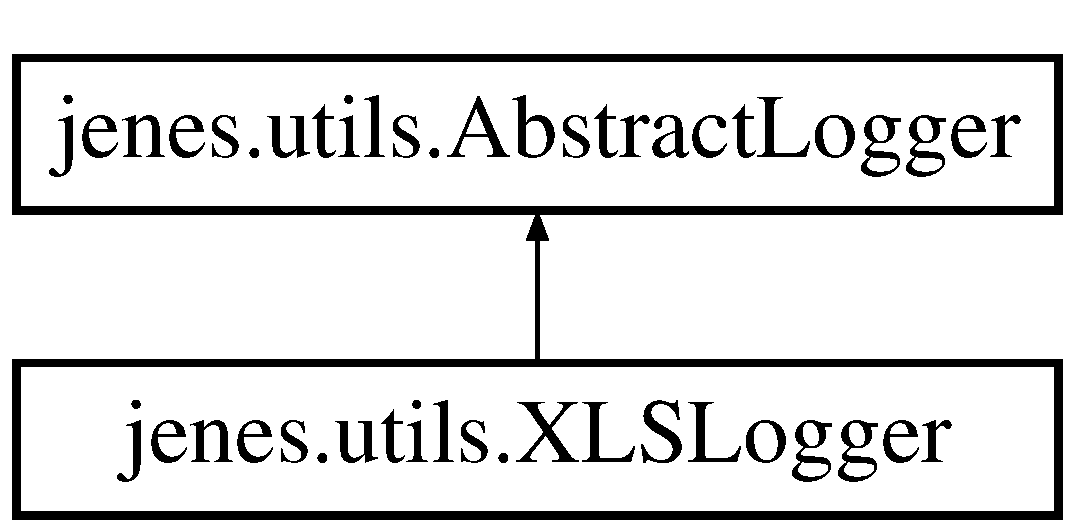
\includegraphics[height=2cm]{classjenes_1_1utils_1_1_x_l_s_logger}
\end{center}
\end{figure}
\subsection*{Public Member Functions}
\begin{CompactItemize}
\item 
\hyperlink{classjenes_1_1utils_1_1_x_l_s_logger_1fa625f6c332aca9178b1c7a4eb963d8}{XLSLogger} (String\mbox{[}$\,$\mbox{]} \hyperlink{classjenes_1_1utils_1_1_abstract_logger_3a2030876857a0512fae7e0ad400c570}{schema})  throws IOException 
\item 
\hyperlink{classjenes_1_1utils_1_1_x_l_s_logger_256b5ddf3beaa1eedb2290b52bb1a845}{XLSLogger} (String\mbox{[}$\,$\mbox{]} \hyperlink{classjenes_1_1utils_1_1_abstract_logger_3a2030876857a0512fae7e0ad400c570}{schema}, String filename)  throws IOException 
\item 
\hyperlink{classjenes_1_1utils_1_1_x_l_s_logger_c43b3385840e86a2ad4acd5040e8326b}{XLSLogger} (String\mbox{[}$\,$\mbox{]} \hyperlink{classjenes_1_1utils_1_1_abstract_logger_3a2030876857a0512fae7e0ad400c570}{schema}, String filename, int from)  throws IOException 
\item 
\hyperlink{classjenes_1_1utils_1_1_x_l_s_logger_2e438a48213dd4e1773c380d7f9d7e4b}{XLSLogger} (String\mbox{[}$\,$\mbox{]} \hyperlink{classjenes_1_1utils_1_1_abstract_logger_3a2030876857a0512fae7e0ad400c570}{schema}, String filename, String template)  throws IOException 
\item 
int \hyperlink{classjenes_1_1utils_1_1_x_l_s_logger_60e8ee28d3d3305e085726026e09cfdc}{getLine} ()
\item 
void \hyperlink{classjenes_1_1utils_1_1_x_l_s_logger_2f9ce5372263fadce99a863149f3cb55}{setLine} (int line)
\item 
WritableWorkbook \hyperlink{classjenes_1_1utils_1_1_x_l_s_logger_b84e4c5e6518902f710cd3c3cc337f3d}{getWorkbook} ()
\end{CompactItemize}
\subsection*{Protected Member Functions}
\begin{CompactItemize}
\item 
void \hyperlink{classjenes_1_1utils_1_1_x_l_s_logger_e6b3840ad6be8bdc558efaf6077d4ae4}{store} ()
\item 
void \hyperlink{classjenes_1_1utils_1_1_x_l_s_logger_54c54393bf5a31442ebfc10517dfceea}{doSave} ()
\item 
void \hyperlink{classjenes_1_1utils_1_1_x_l_s_logger_cf58ddaa6873bcf626c9d24064a89b73}{doClose} ()
\end{CompactItemize}


\subsection{Detailed Description}
This class implements a logger based on Excel's XLS files.

Data are stored in the first column having the data label as header. It does not matter in which sheet. Recording can start from any row. From which row to start recording can be decided at istantiation or execution time.

The class can work with an empty file or with a template provided at instantiation time. Using a template is a helpful with macros and plots, in order to make ready-to-use reports.

Requires the libray JExcelApi.

\begin{Desc}
\item[Version:]2.0 \end{Desc}
\begin{Desc}
\item[Since:]1.3 \end{Desc}


\subsection{Constructor \& Destructor Documentation}
\hypertarget{classjenes_1_1utils_1_1_x_l_s_logger_1fa625f6c332aca9178b1c7a4eb963d8}{
\index{jenes::utils::XLSLogger@{jenes::utils::XLSLogger}!XLSLogger@{XLSLogger}}
\index{XLSLogger@{XLSLogger}!jenes::utils::XLSLogger@{jenes::utils::XLSLogger}}
\subsubsection[XLSLogger]{\setlength{\rightskip}{0pt plus 5cm}jenes.utils.XLSLogger.XLSLogger (String\mbox{[}$\,$\mbox{]} {\em schema})  throws IOException }}
\label{classjenes_1_1utils_1_1_x_l_s_logger_1fa625f6c332aca9178b1c7a4eb963d8}


Istantiates a new logger with a given schema. Data are saved by defualt in the workbook jenes.log.xls. Recording starts from row 1.

\begin{Desc}
\item[Parameters:]
\begin{description}
\item[{\em schema}]- the field labels \end{description}
\end{Desc}
\begin{Desc}
\item[Exceptions:]
\begin{description}
\item[{\em IOException}]\end{description}
\end{Desc}
\hypertarget{classjenes_1_1utils_1_1_x_l_s_logger_256b5ddf3beaa1eedb2290b52bb1a845}{
\index{jenes::utils::XLSLogger@{jenes::utils::XLSLogger}!XLSLogger@{XLSLogger}}
\index{XLSLogger@{XLSLogger}!jenes::utils::XLSLogger@{jenes::utils::XLSLogger}}
\subsubsection[XLSLogger]{\setlength{\rightskip}{0pt plus 5cm}jenes.utils.XLSLogger.XLSLogger (String\mbox{[}$\,$\mbox{]} {\em schema}, \/  String {\em filename})  throws IOException }}
\label{classjenes_1_1utils_1_1_x_l_s_logger_256b5ddf3beaa1eedb2290b52bb1a845}


Istantiates a new logger with a given schema. Recording starts from row 1.

\begin{Desc}
\item[Parameters:]
\begin{description}
\item[{\em schema}]- the field labels \item[{\em filename}]- the workbook filename \end{description}
\end{Desc}
\begin{Desc}
\item[Exceptions:]
\begin{description}
\item[{\em IOException}]\end{description}
\end{Desc}
\hypertarget{classjenes_1_1utils_1_1_x_l_s_logger_c43b3385840e86a2ad4acd5040e8326b}{
\index{jenes::utils::XLSLogger@{jenes::utils::XLSLogger}!XLSLogger@{XLSLogger}}
\index{XLSLogger@{XLSLogger}!jenes::utils::XLSLogger@{jenes::utils::XLSLogger}}
\subsubsection[XLSLogger]{\setlength{\rightskip}{0pt plus 5cm}jenes.utils.XLSLogger.XLSLogger (String\mbox{[}$\,$\mbox{]} {\em schema}, \/  String {\em filename}, \/  int {\em from})  throws IOException }}
\label{classjenes_1_1utils_1_1_x_l_s_logger_c43b3385840e86a2ad4acd5040e8326b}


Istantiates a new logger with a given schema.

\begin{Desc}
\item[Parameters:]
\begin{description}
\item[{\em schema}]- the field labels \item[{\em filename}]- the workbook filename \item[{\em from}]- the recording initial row \end{description}
\end{Desc}
\begin{Desc}
\item[Exceptions:]
\begin{description}
\item[{\em IOException}]\end{description}
\end{Desc}
\hypertarget{classjenes_1_1utils_1_1_x_l_s_logger_2e438a48213dd4e1773c380d7f9d7e4b}{
\index{jenes::utils::XLSLogger@{jenes::utils::XLSLogger}!XLSLogger@{XLSLogger}}
\index{XLSLogger@{XLSLogger}!jenes::utils::XLSLogger@{jenes::utils::XLSLogger}}
\subsubsection[XLSLogger]{\setlength{\rightskip}{0pt plus 5cm}jenes.utils.XLSLogger.XLSLogger (String\mbox{[}$\,$\mbox{]} {\em schema}, \/  String {\em filename}, \/  String {\em template})  throws IOException }}
\label{classjenes_1_1utils_1_1_x_l_s_logger_2e438a48213dd4e1773c380d7f9d7e4b}


Istantiates a new logger with a given schema. Recording starts from row 1.

\begin{Desc}
\item[Parameters:]
\begin{description}
\item[{\em schema}]- the field labels \item[{\em filename}]- the workbook name \item[{\em template}]- the workbook template \end{description}
\end{Desc}
\begin{Desc}
\item[Exceptions:]
\begin{description}
\item[{\em IOException}]\end{description}
\end{Desc}


\subsection{Member Function Documentation}
\hypertarget{classjenes_1_1utils_1_1_x_l_s_logger_60e8ee28d3d3305e085726026e09cfdc}{
\index{jenes::utils::XLSLogger@{jenes::utils::XLSLogger}!getLine@{getLine}}
\index{getLine@{getLine}!jenes::utils::XLSLogger@{jenes::utils::XLSLogger}}
\subsubsection[getLine]{\setlength{\rightskip}{0pt plus 5cm}int jenes.utils.XLSLogger.getLine ()}}
\label{classjenes_1_1utils_1_1_x_l_s_logger_60e8ee28d3d3305e085726026e09cfdc}


Provides the current recording row

\begin{Desc}
\item[Returns:]- recording row \end{Desc}
\hypertarget{classjenes_1_1utils_1_1_x_l_s_logger_2f9ce5372263fadce99a863149f3cb55}{
\index{jenes::utils::XLSLogger@{jenes::utils::XLSLogger}!setLine@{setLine}}
\index{setLine@{setLine}!jenes::utils::XLSLogger@{jenes::utils::XLSLogger}}
\subsubsection[setLine]{\setlength{\rightskip}{0pt plus 5cm}void jenes.utils.XLSLogger.setLine (int {\em line})}}
\label{classjenes_1_1utils_1_1_x_l_s_logger_2f9ce5372263fadce99a863149f3cb55}


Sets the current recording row at a specified value.

\begin{Desc}
\item[Parameters:]
\begin{description}
\item[{\em line}]- the new recording row \end{description}
\end{Desc}
\hypertarget{classjenes_1_1utils_1_1_x_l_s_logger_b84e4c5e6518902f710cd3c3cc337f3d}{
\index{jenes::utils::XLSLogger@{jenes::utils::XLSLogger}!getWorkbook@{getWorkbook}}
\index{getWorkbook@{getWorkbook}!jenes::utils::XLSLogger@{jenes::utils::XLSLogger}}
\subsubsection[getWorkbook]{\setlength{\rightskip}{0pt plus 5cm}WritableWorkbook jenes.utils.XLSLogger.getWorkbook ()}}
\label{classjenes_1_1utils_1_1_x_l_s_logger_b84e4c5e6518902f710cd3c3cc337f3d}


Rovides the workbook used for writing the statistics. See JExcelApi documentation for futher information.

\begin{Desc}
\item[Returns:]the workbook \end{Desc}
\hypertarget{classjenes_1_1utils_1_1_x_l_s_logger_e6b3840ad6be8bdc558efaf6077d4ae4}{
\index{jenes::utils::XLSLogger@{jenes::utils::XLSLogger}!store@{store}}
\index{store@{store}!jenes::utils::XLSLogger@{jenes::utils::XLSLogger}}
\subsubsection[store]{\setlength{\rightskip}{0pt plus 5cm}void jenes.utils.XLSLogger.store ()\hspace{0.3cm}{\tt  \mbox{[}protected, virtual\mbox{]}}}}
\label{classjenes_1_1utils_1_1_x_l_s_logger_e6b3840ad6be8bdc558efaf6077d4ae4}


Stores the current record. 

Implements \hyperlink{classjenes_1_1utils_1_1_abstract_logger_6acf83a83999e26ae4ed45cbf355111b}{jenes.utils.AbstractLogger}.\hypertarget{classjenes_1_1utils_1_1_x_l_s_logger_54c54393bf5a31442ebfc10517dfceea}{
\index{jenes::utils::XLSLogger@{jenes::utils::XLSLogger}!doSave@{doSave}}
\index{doSave@{doSave}!jenes::utils::XLSLogger@{jenes::utils::XLSLogger}}
\subsubsection[doSave]{\setlength{\rightskip}{0pt plus 5cm}void jenes.utils.XLSLogger.doSave ()\hspace{0.3cm}{\tt  \mbox{[}protected, virtual\mbox{]}}}}
\label{classjenes_1_1utils_1_1_x_l_s_logger_54c54393bf5a31442ebfc10517dfceea}


Saves cached records on media 

Implements \hyperlink{classjenes_1_1utils_1_1_abstract_logger_41fcd50b050c467fe1b413fc5b49c167}{jenes.utils.AbstractLogger}.\hypertarget{classjenes_1_1utils_1_1_x_l_s_logger_cf58ddaa6873bcf626c9d24064a89b73}{
\index{jenes::utils::XLSLogger@{jenes::utils::XLSLogger}!doClose@{doClose}}
\index{doClose@{doClose}!jenes::utils::XLSLogger@{jenes::utils::XLSLogger}}
\subsubsection[doClose]{\setlength{\rightskip}{0pt plus 5cm}void jenes.utils.XLSLogger.doClose ()\hspace{0.3cm}{\tt  \mbox{[}protected, virtual\mbox{]}}}}
\label{classjenes_1_1utils_1_1_x_l_s_logger_cf58ddaa6873bcf626c9d24064a89b73}


Closes the logger. Any further log is not allowed. 

Implements \hyperlink{classjenes_1_1utils_1_1_abstract_logger_5253672b3f3f81287db2fc604ca921a9}{jenes.utils.AbstractLogger}.

The documentation for this class was generated from the following file:\begin{CompactItemize}
\item 
src/jenes/utils/XLSLogger.java\end{CompactItemize}

\printindex
\end{document}
